\documentclass[aspectratio = 169]{beamer}

\usepackage{../common/beamerthemedarc}
\PassOptionsToPackage{fleqn}{amsmath}
\usepackage{amsmath}
\usepackage{amssymb}
\usepackage{csquotes}
\usepackage[greek,german]{babel}
\usepackage{siunitx}
\usepackage{tabularray}
\usepackage{fontawesome5}
\usepackage{cancel}
\makeatletter
\let\ang\relax
\makeatother
\usepackage{texvc}

\DeclareSIUnit{\baud}{Bd}
\DeclareSIUnit{\dBi}{dBi}
\DeclareSIUnit{\dBm}{dBm}
\DeclareSIUnit{\dBu}{dBu}
\DeclareSIUnit{\dBV}{dbV}
\DeclareSIUnit{\dBW}{dBW}
\DeclareSIUnit{\ppm}{ppm}
\DeclareSIUnit{\pps}{pps}
\DeclareSIUnit{\CPM}{CPM}
\DeclareSIUnit{\WPM}{WPM}
\DeclareSIUnit\noop{\relax}

\definecolor{DARCgreen}{RGB}{0,155,110}
\definecolor{DARCorange}{RGB}{250,180,0}
\definecolor{DARCred}{RGB}{225,80,35}
\definecolor{DARCblue}{RGB}{0,160,220}
\definecolor{DARCgray}{RGB}{190,190,190}
\definecolor{DARClightgray}{HTML/cmyk}{e8e9e8/.11,.07,.09,0}

\definecolor{unit-title}{RGB}{155,205,185}
\definecolor{attention-title}{RGB}{255,230,170}
\definecolor{danger-title}{RGB}{245,175,150}
\definecolor{hint-title}{RGB}{185,220,245}
\definecolor{advanced-title}{RGB}{225,230,235}

\definecolor{DARCdarkblue}{RGB}{43, 103, 140}

\definecolor{r}{rgb}{0.98, 0.84, 0.65}
\definecolor{rsilver}{rgb}{0.75, 0.75, 0.75}
\definecolor{rgold}{rgb}{0.85, 0.65, 0.13}
\definecolor{rbrown}{rgb}{0.59, 0.29, 0.0}
\definecolor{rblack}{rgb}{0,0,0}
\definecolor{rred}{rgb}{0.89, 0.0, 0.13}
\definecolor{rorange}{rgb}{0.93, 0.53, 0.18}
\definecolor{ryellow}{rgb}{1.0, 0.96, 0.0}
\definecolor{rgreen}{rgb}{0.0, 0.42, 0.24}
\definecolor{rblue}{rgb}{0.06, 0.2, 0.65}
\definecolor{rviolet}{rgb}{0.56, 0.0, 1.0}
\definecolor{rgrey}{rgb}{0.33, 0.33, 0.33}
\definecolor{rwhite}{rgb}{0.96, 0.96, 0.96}

\tcbset{QSO/.style={
	enhanced,boxrule=0pt,
	frame empty,colback=DARClightgray,fontupper=\footnotesize,
	interior code={
		\fill[tcbcolback](frame.north west)to(frame.north east)to([yshift=-\ht\strutbox]interior.north east)to(interior.south east)to(interior.south west)to([yshift=-\ht\strutbox]interior.north west)--cycle;
	}
}}

\newcommand{\QSOown}[1]{\begin{tcolorbox}[
		QSO,
		leftrule=\ht\strutbox,
		right skip=.1\linewidth
]%
#1%
\end{tcolorbox}}

\newcommand{\QSOother}[1]{\begin{tcolorbox}[
		QSO,
		rightrule=\ht\strutbox,
		left skip=.1\linewidth]%
		#1%
\end{tcolorbox}}

\newenvironment{QQuestion}[6]{
    \begin{block}{#1}
        #2
        \begin{itemize}
            \item[A:] #3
            \item[B:] #4
            \item[C:] #5
            \item[D:] #6
        \end{itemize}
    \end{block}
}

\newenvironment{PQuestion}[7]{
    \begin{block}{#1}
        \begin{columns}
            \begin{column}{0.48\linewidth}
                #7
            \end{column}
            \begin{column}{0.48\linewidth}
                #2
                \begin{itemize}
                    \item[A:] #3
                    \item[B:] #4
                    \item[C:] #5
                    \item[D:] #6
                \end{itemize}
            \end{column}
        \end{columns}
    \end{block}
}

\newenvironment{question_md}[6]{
    \Question{#1}{#2}{#3}{#4}{#5}{#6}
}

\newenvironment{question2x2}[6]{
    \begin{block}{#1}
        #2
        \begin{columns}
            \begin{column}{0.48\linewidth}
                \begin{itemize}
                    \item[A:] #3
                    \item[B:] #4
                \end{itemize}
            \end{column}
            \begin{column}{0.48\linewidth}
                \begin{itemize}
                    \item[C:] #5
                    \item[D:] #6
                \end{itemize}
            \end{column}
        \end{columns}
    \end{block}
}

%\newenvironment{DARCtabular}[1]{
%    \begin{tblr}{hlines, colspec={#1}}
%}{
%    \end{tblr}
%}

\NewTblrEnviron{DARCtabular}

\SetTblrInner[DARCtabular]{
    row{odd} = {DARCblue!30},
    row{even} = {DARCblue!50},
    row{1} = {bg=DARCblue, fg=white, font=\bfseries}
}

\SetTblrOuter[DARCtabular]{
    baseline=B
}

\PassOptionsToPackage{locale=DE}{siunitx}
\PassOptionsToPackage{straightvoltages, europeanresistors, european inductor}{circuitikz}

\usepackage[locale=DE]{siunitx}
\usepackage{ifthen}
\usepackage{mathtools}
\usepackage{unicode-math}
\setmathfont{Libertinus Math}

\usepackage{circuitikz}
\makeatletter
\let\empty\relax
\makeatother
\usepackage{pgfplots}
\usepackage{pgfmath}
\usepackage{pgfplotstable}

\usepackage{etoolbox}
\usepackage{xcolor}
\usepackage{MnSymbol}

\usepackage{wasysym}
\usepackage{tikz-dimline}
\AtBeginDocument{\RenewCommandCopy\qty\SI} % Fix um qty doppeldefinition zu vermeiden 
\usepackage{tikz-3dplot}
%\usepackage{filecontents}% removed as obsolete

%TODO remove?
\usepackage{varwidth}
\usepackage{pgf-spectra}
\usepgfspectralibrary{pgfplots}

% TODO
% hier mal hart forciert, weil if ggf nicht geht?
% define colormap and check if cmyk is enforced
%\def\test#1{cmyk}
%\ifx\XC@tgt@mod\test
%	\pgfplotsset{colormap={slategraywhite}{cmyk=(0,0,0,.8) cmyk=(0,0,0,0)}}
%\else
	\pgfplotsset{colormap={slategraywhite}{rgb255=(50,50,50) rgb255=(255,255,255)}}
%\fi


\usetikzlibrary{math,perspective,intersections,arrows,arrows.meta,positioning,calc,shapes.symbols,decorations.pathmorphing,patterns,shapes.geometric,matrix,3d,backgrounds,babel,pgfplots.polar,decorations.pathreplacing,calligraphy,decorations.text,svg.path,optics}
\usepgfplotslibrary{fillbetween}
\pgfplotsset{compat=1.18}
\DeclareSIUnit{\baud}{Bd}

\sisetup{
    range-phrase=--,
    range-units=single
}

\usepackage[euler]{textgreek}

% Setze die Enden der optischen Pfeile etc. auf 60 grad:
\ctikzset{
	opto end arrow={Triangle[angle'=60]},
	tunable end arrow={Triangle}
}

% Grundsätzlich alle Pfeile als Triangle TODO, danach suchen und dann loeschen!
\tikzset{
    myarrow/.style={-Triangle}
}
\ctikzset{
    resistor=european,
    voltage=straight
}

\tikzstyle{digitalNumber}=[draw=DARCgray, fill=white, minimum width=0.5, minimum height=0.5, rounded corners=1, font=\bfseries]

% Gekritzelte Linie (Bild 315)
\pgfdeclaredecoration{penciline}{initial}{
	\state{initial}[width=+\pgfdecoratedinputsegmentremainingdistance,
	auto corner on length=1mm,]{
		\pgfpathcurveto%
		{% From
			\pgfqpoint{\pgfdecoratedinputsegmentremainingdistance}
			{\pgfdecorationsegmentamplitude}
		}
		{%  Control 1
			\pgfmathrand
			\pgfpointadd{\pgfqpoint{\pgfdecoratedinputsegmentremainingdistance}{0pt}}
			{\pgfqpoint{-\pgfdecorationsegmentaspect
					\pgfdecoratedinputsegmentremainingdistance}%
				{\pgfmathresult\pgfdecorationsegmentamplitude}
			}
		}
		{%TO
			\pgfpointadd{\pgfpointdecoratedinputsegmentlast}{\pgfpoint{1pt}{1pt}}
		}
	}
	\state{final}{}
}

% Bandplan bänder in Bild 750 und 749
\let\band\relax% conflict… requires cleanup … \providecommand? 
\newcommand{\band}[7]{%
    \draw[draw=red] (-5,#1) rectangle (5,#2);
    \draw ( 40,#1) node[right,rotate=0, text=red](){\footnotesize\textbf{\SI{#6}{#7}}};
    \draw ( 20,#1) node[rotate=0](){\footnotesize\SI{#3}{#5}};
    \draw (-20,#2) node[rotate=0](){\footnotesize\SI{#4}{#5}};
}

\let\bandB\relax% conflict… requires cleanup … \providecommand? 
\newcommand{\bandB}[7]{%
    \draw[draw=red] (-5,#1) rectangle (5,#2);
    \draw ( 40,#1) node[right,rotate=0, text=red](){\footnotesize\textbf{\SI{#6}{#7}}};
    \draw ( 20,#1) node[rotate=0,above](){\footnotesize\SI{#3}{#5}};
    \draw (-20,#2) node[rotate=0,above](){\footnotesize\SI{#4}{#5}};
}

\newcommand{\bandC}[7]{%
    \draw[draw=red] (#1,-5) rectangle (#2,5);
    \draw (#1, 65.0) node[rotate=-90, text=red](){\footnotesize\textbf{\SI{#6}{#7}}};
    \draw (#1, 27.5) node[rotate=-90](){\footnotesize\SI{#3}{#5}};
    \draw (#2,-27.5) node[rotate=-90](){\footnotesize\SI{#4}{#5}};
}

\newcommand{\bandD}[5]{%
    \draw[draw=red] (#1,-5) rectangle (#2,5);
    \draw (#1+50000000, 27.5) node[rotate=-90](){\footnotesize\SI{#3}{#5}};
    \draw (#2+50000000,-27.5) node[rotate=-90](){\footnotesize\SI{#4}{#5}};
}

% Symbol für das Gleichstrom
\newcommand{\textdirectcurrent}{%
  \settowidth{\dimen0}{$=$}%
  \vbox to .85ex {\offinterlineskip
    \hbox to \dimen0{\leaders\hrule\hfill}
    \vskip.35ex
    \hbox to \dimen0{%
      \leaders\hrule\hskip.2\dimen0\hfill
      \leaders\hrule\hskip.2\dimen0\hfill
      \leaders\hrule\hskip.2\dimen0
    }
    \vfill
  }%
}
\newcommand{\mathdirectcurrent}{\mathrel{\textdirectcurrent}}

% Zum Messen von Abständen
\makeatletter
\newcommand{\Distance}[3]{% from https://tex.stackexchange.com/q/56353/121799
	\tikz@scan@one@point\pgfutil@firstofone($#1-#2$)\relax  
	\pgfmathsetmacro{#3}{round(0.99626*veclen(\the\pgf@x,\the\pgf@y)/0.0283465)/1000}
}
\makeatother

% Bemaßung zeichnen:
\NewDocumentCommand\DARCmeasure{O{black} O{middle} m m m m m}{% 1:[color], 2:[top], 3:start, 4:end, 5:shift, 6:rotate, 7:text
    \path($(#3)+(#5)$) coordinate(start);
    \path($(#4)+(#5)$) coordinate(end);
    \ifthenelse{\equal{#2}{top}}{
        \draw ($(start)!0.5!(end)$) coordinate(middle);
        \node[rotate=#6, anchor=south] (text) at (middle) {\textcolor{#1}{#7}};
        \draw[draw=#1, |Triangle-] (start) -- (middle);
        \draw[draw=#1, |Triangle-] (end) -- (middle);
    }{
        \node[rotate=#6] (text) at ($(start)!0.5!(end)$) {\textcolor{#1}{#7}};
        \draw[draw=#1, |Triangle-] (start) -- (text.west);
        \draw[draw=#1, |Triangle-] (end) -- (text.east);
    }
}

% Magic von Marei zur Skalierung der Bilder
\makeatletter
\ExplSyntaxOn
\box_new:N \l_ptxcd_image_box

\cs_if_exist:NF \if@DARCinQuestion {\newif\if@DARCinQuestion}

\fp_if_exist:NF \l_ptxcd_tmp_fp {\fp_new:N \l_ptxcd_tmp_fp}
\fp_set:Nn \l_ptxcd_tmp_fp  {1}

\int_new:N \g_DARC_image_fail_int
\seq_new:N \g__DARC_image_fail_seq
\dim_new:N \l__DARC_image_width_dim
\box_new:N \l_ptxcd_image_orig_box

\newcommand*{\getDarcImageFactor}{\fp_use:N  \l_ptxcd_tmp_fp}



\NewDocumentCommand{\DARCimageOnly}{smm}{
	\setmathfont{Libertinus Math}
	 \ptxcd_image_autoscale_setup:nnn {#1} {#2} {#3}
		\usepackage{geometry}
        \usepackage{}
	\geometry{paperwidth=\box_wd:N  \l_ptxcd_image_box, paperheight=\box_ht_plus_dp:N  \l_ptxcd_image_box,margin=0pt}
	\pagestyle{empty}
	\setlength{\topskip}{0pt}% necessary because otherwhise \topskip could exceed \paperheight
	\begin{document}
		\box_use:N \l_ptxcd_image_box
	\end{document}
}

\seq_new:N  \g__ptxcd_image_size_seq
\prop_new:N \g__ptxcd_image_size_cache_prop
\bool_new:N \l__ptxcd_disable_autoscale_bool
\newcommand*{\disableDARCautoscale}{\bool_set_true:N  \l__ptxcd_disable_autoscale_bool}

\cs_new:Nn \ptxcd_image_autoscale_setup:nnn {
	\prop_if_in:NnTF \g__ptxcd_image_size_cache_prop {#2} {
			\fp_set:Nn \l_ptxcd_tmp_fp {\prop_item:Nn \g__ptxcd_image_size_cache_prop {#2}}
			\hbox_gset:Nn \l_ptxcd_image_box {
				\tikzset{x=\fp_use:N \l_ptxcd_tmp_fp cm,y=\fp_use:N \l_ptxcd_tmp_fp cm}
				\file_if_exist_input:n {img/#2}%
				\ifvmode\else\unskip\fi
			}
		\seq_gput_right:Nx \g__ptxcd_image_size_seq {#2=\prop_item:Nn \g__ptxcd_image_size_cache_prop {#2}}
	} {
		\hbox_gset:Nn \l_ptxcd_image_orig_box {
			\file_if_exist_input:n {img/#3}%
			\ifvmode\else\unskip\fi%
		}
		\bool_if:NT \l__ptxcd_disable_autoscale_bool \use_iii:nnnn
		\IfBooleanTF{#1}{
			\box_gset_eq:NN \l_ptxcd_image_box \l_ptxcd_image_orig_box
		} {
			\dim_compare:nNnTF {\box_wd:N \l_ptxcd_image_orig_box} = {\c_zero_dim} {
				\fp_set:Nn  \l_ptxcd_tmp_fp {1}
			} {
				\if@DARCinQuestion
					\dim_compare:nTF {#2 =\linewidth} {
						\dim_set:Nn  \l__DARC_image_width_dim {\columnwidth}
					} {
						\dim_set:Nn  \l__DARC_image_width_dim {#2}
					}
				\else
					\dim_set:Nn  \l__DARC_image_width_dim {#2}
				\fi
				\fp_set:Nn \l_ptxcd_tmp_fp {\dim_to_decimal_in_unit:nn {\l__DARC_image_width_dim} {\box_wd:N \l_ptxcd_image_orig_box}}
				\hbox_gset:Nn \l_ptxcd_image_box {
					\tikzset{x=\fp_use:N \l_ptxcd_tmp_fp cm,y=\fp_use:N \l_ptxcd_tmp_fp cm}
					\file_if_exist_input:n {img/#3}%
					\ifvmode\else\unskip\fi
				}
				\bool_lazy_and:nnT
					{ \dim_compare_p:nNn {\box_wd:N \l_ptxcd_image_box} < {\l__DARC_image_width_dim  -1em} }
					{ ! \dim_compare_p:nNn {\box_wd:N \l_ptxcd_image_box} = {\box_wd:N \l_ptxcd_image_orig_box}}
				{
					\fp_set:Nn \l_ptxcd_tmp_fp { 1 + \dim_to_decimal_in_unit:nn {\l__DARC_image_width_dim- \box_wd:N \l_ptxcd_image_orig_box} {\box_wd:N \l_ptxcd_image_box - \box_wd:N \l_ptxcd_image_orig_box} * (\l_ptxcd_tmp_fp  -1)}
					\hbox_gset:Nn \l_ptxcd_image_box {
						\tikzset{x=\fp_use:N \l_ptxcd_tmp_fp cm,y=\fp_use:N \l_ptxcd_tmp_fp cm}
						\file_if_exist_input:n {img/#3}%
						\ifvmode\else\unskip\fi
					}
				}
				\dim_compare:nNnTF  {\box_wd:N \l_ptxcd_image_box} = {\box_wd:N \l_ptxcd_image_orig_box} {
					\seq_gput_right:Nx \g__ptxcd_image_size_seq {#3=1}
				}{
					\seq_gput_right:Nx \g__ptxcd_image_size_seq {#3=\fp_use:N \l_ptxcd_tmp_fp}
				}
			}
		}
	}
}

\newcommand*{\DARCimageCache}[1]{
	\prop_gset_from_keyval:Nn \g__ptxcd_image_size_cache_prop {#1}
}

\hook_gput_code:nnn {enddocument/afterlastpage}{write-DARCimage-size-cache}{
	\iow_now:Ne \@auxout {
		\exp_not:N \DARCimageCache{
			\seq_use:Nn  \g__ptxcd_image_size_seq {,}
		}
	}
}

\NewDocumentCommand{\DARCimage}{sO{Bild~zur~Prüfungsfrage~\l_ptxcd_question_tl}mm}{
	\par\smallskip
	\begingroup
		\ptxcd_image_autoscale_setup:nnn {#1} {#3} {#4}
		\dim_compare:nNnTF {\box_wd:N \l_ptxcd_image_box} > {\linewidth}
		{
			\makebox[\linewidth][r]{\box_use:N \l_ptxcd_image_box}
		} {
			\makebox[\linewidth][c]{\box_use:N \l_ptxcd_image_box}
		}
	\endgroup
}
\ExplSyntaxOff
\makeatother

% Neue TL, wird bald in einem zukünftigen circuittikz sein: 
% https://github.com/circuitikz/circuitikz/issues/694
\makeatletter
\newif\ifpgf@circ@bare@tline
\ctikzset{bipoles/tline/bare/.is if=pgf@circ@bare@tline}
\pgfcircdeclarebipolescaled{RF}
{
\savedmacro{\recessright}{\edef\recessright{\ifpgf@circ@bare@tline -0.4\else 0.0\fi}}
\anchor{center right}{\northeast \advance\pgf@x by -0.4\pgf@y\pgf@y=0pt}
\anchor{top right}{\northeast \advance\pgf@x by -0.4\pgf@y}
\anchor{bottom right}{\northeast \advance\pgf@x by -0.4\pgf@y\pgf@y=-\pgf@y}
\anchor{center left}{\northeast \advance\pgf@x by -0.4\pgf@y\pgf@x=-\pgf@x\pgf@y=0pt}
\anchor{top left}{\northeast \advance\pgf@x by -0.4\pgf@y\pgf@x=-\pgf@x}
\anchor{bottom left}{\northeast \advance\pgf@x by -0.4\pgf@y\pgf@x=-\pgf@x\pgf@y=-\pgf@y}
\anchor{right}{\northeast \advance\pgf@x by \recessright\pgf@y\pgf@y=0pt}
}
{\ctikzvalof{bipoles/tline/height}}
{tline}
{\ctikzvalof{bipoles/tline/height}}
{\ctikzvalof{bipoles/tline/width}}
{
\pgf@circ@res@step=.4\pgf@circ@res@up % the size of the ellipsis is proportional to the height
\pgfscope
\pgf@circ@setlinewidth{bipoles}{\pgfstartlinewidth}
\pgfpathmoveto{\pgfpoint{\pgf@circ@res@right-\pgf@circ@res@step}{\pgf@circ@res@up}}
\pgfpathlineto{\pgfpoint{\pgf@circ@res@left+\pgf@circ@res@step}{\pgf@circ@res@up}}
\pgfpatharc{-90}{90}{-\pgf@circ@res@step and -\pgf@circ@res@up}
\pgfpathlineto{\pgfpoint{\pgf@circ@res@right-\pgf@circ@res@step}{\pgf@circ@res@down}}
\pgfpatharc{-90}{90}{\pgf@circ@res@step and \pgf@circ@res@up}
\pgf@circ@draworfill
\pgfpathmoveto{\pgfpoint{\pgf@circ@res@right-\pgf@circ@res@step}{\pgf@circ@res@up}}
\pgfpatharc{-90}{90}{-\pgf@circ@res@step and -\pgf@circ@res@up}
\pgfusepath{stroke}
\endpgfscope
\ifpgf@circ@bare@tline\else
\pgfsetlinewidth{\pgfstartlinewidth}
\pgfpathmoveto{\pgfpoint{\pgf@circ@res@right-\pgf@circ@res@step}{0pt}}
\pgfpathlineto{\pgfpoint{\pgf@circ@res@right}{0pt}}
\pgfusepath{stroke}
\fi
}
\makeatother

% Neues mikrofon, wird irgendwann teil von circuit tikzi und kann dann hier
% gelöscht werden: https://github.com/circuitikz/circuitikz/issues/689
% <
\makeatletter
\ctikzset{bipoles/tlmic/height/.initial=.5}
\ctikzset{bipoles/tlmic/depth/.initial=.5}
\ctikzset{bipoles/tlmic/width/.initial=.5}%
\pgfcircdeclarebipolescaled{misc}
{}
{\ctikzvalof{bipoles/tlmic/depth}}
{tlmic}
{\ctikzvalof{bipoles/tlmic/height}}
{\ctikzvalof{bipoles/tlmic/width}}{

    \pgf@circ@setlinewidth{bipoles}{\pgfstartlinewidth}
    \pgfpathcircle{\pgfpoint{0pt}{0pt}}{\pgf@circ@res@up}
    \pgf@circ@draworfill
    \pgfpathmoveto{\pgfpoint{\pgf@circ@res@left}{\pgf@circ@res@up}}
    \pgfpathlineto{\pgfpoint{\pgf@circ@res@right}{\pgf@circ@res@up}}
    \pgfusepath{draw}
}
\pgfcirc@activate@bipole@simple{l}{tlmic}

\makeatother
% />

% Power Plug
\makeatletter
\ctikzset{bipoles/plug/height/.initial=.5}
\ctikzset{bipoles/plug/width/.initial=.5}%
\pgfcircdeclarebipolescaled{misc}
{}
{\ctikzvalof{bipoles/plug/height}}
{plug}
{\ctikzvalof{bipoles/plug/height}}
{\ctikzvalof{bipoles/plug/width}}{

    %\pgf@circ@setlinewidth{bipoles}{\pgfstartlinewidth}
    \pgfpathcircle{\pgfpoint{0pt}{0pt}}{\pgf@circ@res@up}
	\pgfusepath{fill}
    %\pgfpathmoveto{\pgfpoint{\pgf@circ@res@left}{\pgf@circ@res@up}}
    %\pgfpathlineto{\pgfpoint{\pgf@circ@res@right}{\pgf@circ@res@up}}
    %\pgfusepath{draw}
	% Plus:
	\color{black} 
	\pgfsetstrokecolor{black} 
	\pgfpathrectangle{\pgfpoint{0.0\pgf@circ@res@step}{-0.1\pgf@circ@res@step}}{\pgfpoint{-0.2\pgf@circ@res@step}{+0.1\pgf@circ@res@step}}%
	\pgfusepath{fill}
}
\pgfcirc@activate@bipole@simple{l}{plug}
\makeatother

%% bgenerator und bgeneratorshape block
% Eine submission nach circuittikz wurde durchgeführt: 
% https://github.com/circuitikz/circuitikz/pull/693
% <
\makeatletter
%
\def\pgfcirc@twoport@draw@narrowsine#1{% #1 -> y shift
    \pgfscope
        \pgfsetlinewidth{\pgfstartlinewidth}
        \pgftransformyshift{#1\pgf@circ@res@step}
        \pgfpathmoveto{\pgfpoint{.125\pgf@circ@res@step}{0\pgf@circ@res@step}}
        \pgfpathsine{\pgfpoint{.125\pgf@circ@res@step}{.125\pgf@circ@res@step}}
        \pgfpathcosine{\pgfpoint{.125\pgf@circ@res@step}{-.125\pgf@circ@res@step}}
        \pgfpathsine{\pgfpoint{.125\pgf@circ@res@step}{-.125\pgf@circ@res@step}}
        \pgfpathcosine{\pgfpoint{.125\pgf@circ@res@step}{.125\pgf@circ@res@step}}
        \pgfusepath{draw}
    \endpgfscope
}
%
\ctikzset{bipoles/bgenerator/width/.initial=.7}
\pgfcirc@define@twoports{blocks}
{}
{\ctikzvalof{bipoles/bgenerator/width}}
{bgenerator}
{\ctikzvalof{bipoles/bgenerator/width}}
{\ctikzvalof{bipoles/bgenerator/width}}
{
    \pgfcirc@twoport@draw@narrowsine{0.25}{0}
    \pgfcirc@twoport@draw@narrowsine{0.0}{0}
    \pgfcirc@twoport@draw@narrowsine{-0.25}{0}
    \pgftext[x=0.45\pgf@circ@res@left]{\ctikzvalof{bipoles/twoport/text}}
}
\pgfcirc@activate@bipole@simple{l}{bgenerator}
\makeatother
%>

%Q-Generator TODO: Update pull request
\makeatletter
%
\ctikzset{bipoles/qgenerator/width/.initial=.7}
\pgfcirc@define@twoports{blocks}
{}
{\ctikzvalof{bipoles/qgenerator/width}}
{qgenerator}
{\ctikzvalof{bipoles/qgenerator/width}}
{\ctikzvalof{bipoles/qgenerator/width}}
{
    \pgfcirc@twoport@draw@narrowsine{0.45}{0}
    \pgfcirc@twoport@draw@narrowsine{0.20}{0}
    \pgfcirc@twoport@draw@narrowsine{-0.05}{0}
    \pgftext[x=0.45\pgf@circ@res@left,y=0.25\pgf@circ@res@up]{\ctikzvalof{bipoles/twoport/text}}
	\pgfpathmoveto{\pgfpoint{-0.7\pgf@circ@res@step}{-0.35\pgf@circ@res@step}} 
	\pgfpathlineto{\pgfpoint{ 0.7\pgf@circ@res@step}{-0.35\pgf@circ@res@step}} 
    \pgfusepath{draw}
	\pgfpathrectangle{\pgfpoint{-0.7\pgf@circ@res@step}{-0.7\pgf@circ@res@step}}{\pgfpoint{1.4\pgf@circ@res@step}{0.2\pgf@circ@res@step}} 
    \pgfusepath{draw}
	\pgfpathmoveto{\pgfpoint{-0.7\pgf@circ@res@step}{-0.85\pgf@circ@res@step}} 
	\pgfpathlineto{\pgfpoint{ 0.7\pgf@circ@res@step}{-0.85\pgf@circ@res@step}} 
    \pgfusepath{draw}
}
\pgfcirc@activate@bipole@simple{l}{qgenerator}
\makeatother

%Clock-Generator TODO: Add to pull request
\makeatletter
%
\ctikzset{bipoles/cgenerator/width/.initial=.7}
\pgfcirc@define@twoports{blocks}
{}
{\ctikzvalof{bipoles/cgenerator/width}}
{cgenerator}
{\ctikzvalof{bipoles/cgenerator/width}}
{\ctikzvalof{bipoles/cgenerator/width}}
{
	\pgfpathmoveto{\pgfpoint{-0.70\pgf@circ@res@step}{-0.35\pgf@circ@res@step}} 
	\pgfpathlineto{\pgfpoint{-0.42\pgf@circ@res@step}{-0.35\pgf@circ@res@step}} 
	\pgfpathlineto{\pgfpoint{-0.42\pgf@circ@res@step}{+0.35\pgf@circ@res@step}} 
	\pgfpathlineto{\pgfpoint{-0.14\pgf@circ@res@step}{+0.35\pgf@circ@res@step}} 
	\pgfpathlineto{\pgfpoint{-0.14\pgf@circ@res@step}{-0.35\pgf@circ@res@step}} 
	\pgfpathlineto{\pgfpoint{+0.14\pgf@circ@res@step}{-0.35\pgf@circ@res@step}} 
	\pgfpathlineto{\pgfpoint{+0.14\pgf@circ@res@step}{+0.35\pgf@circ@res@step}} 
	\pgfpathlineto{\pgfpoint{+0.42\pgf@circ@res@step}{+0.35\pgf@circ@res@step}} 
	\pgfpathlineto{\pgfpoint{+0.42\pgf@circ@res@step}{-0.35\pgf@circ@res@step}} 
	\pgfpathlineto{\pgfpoint{+0.70\pgf@circ@res@step}{-0.35\pgf@circ@res@step}} 
    \pgfusepath{draw}
}
\pgfcirc@activate@bipole@simple{l}{cgenerator}
\makeatother

%Sine Table: TODO in pullrequest packen
\makeatletter
%
\ctikzset{bipoles/sinetable/width/.initial=.7}
\pgfcirc@define@twoports{blocks}
{}
{\ctikzvalof{bipoles/sinetable/width}}
{sinetable}
{\ctikzvalof{bipoles/sinetable/width}}
{\ctikzvalof{bipoles/sinetable/width}}
{
    \pgfcirc@twoport@draw@sine{0.0}{0}
    \pgfcirc@set@arrows{tunable}{}{latex}
	\pgfpathmoveto{\pgfpoint{-0.70\pgf@circ@res@step}{-0.70\pgf@circ@res@step}} 
	\pgfpathlineto{\pgfpoint{+0.70\pgf@circ@res@step}{-0.70\pgf@circ@res@step}} 
    \pgfusepath{draw}
	\pgfpathmoveto{\pgfpoint{-0.70\pgf@circ@res@step}{-0.70\pgf@circ@res@step}} 
	\pgfpathlineto{\pgfpoint{-0.70\pgf@circ@res@step}{+0.70\pgf@circ@res@step}} 
    \pgfusepath{draw}
}
\pgfcirc@activate@bipole@simple{l}{sinetable}
\makeatother

%Sine Table: TODO in pullrequest packen
\makeatletter
%
\ctikzset{bipoles/register/width/.initial=.7}
\pgfcirc@define@twoports{blocks}
{
	\savedanchor\northwest{
		\pgfmathsetlength{\pgf@circ@scaled@Rlen}{\ctikzvalof{\ctikzclass/scale}\pgf@circ@Rlen}
		\pgf@y=\ctikzvalof{bipoles/twoport/width}\pgf@circ@scaled@Rlen
		\pgf@y=.5\pgf@y
		\pgf@x=-\ctikzvalof{bipoles/twoport/width}\pgf@circ@scaled@Rlen
		\pgf@x=.5\pgf@x
	}
	\anchor{clk}{\northwest\pgf@y=0.5\pgf@y}
}
{\ctikzvalof{bipoles/register/width}}
{register}
{\ctikzvalof{bipoles/register/width}}
{\ctikzvalof{bipoles/register/width}}
{
	\pgfpathmoveto{\pgfpoint{-1.00\pgf@circ@res@step}{+0.70\pgf@circ@res@step}} 
	\pgfpathlineto{\pgfpoint{-0.60\pgf@circ@res@step}{+0.50\pgf@circ@res@step}} 
	\pgfpathlineto{\pgfpoint{-1.00\pgf@circ@res@step}{+0.30\pgf@circ@res@step}} 
    \pgfusepath{draw}
}
\pgfcirc@activate@bipole@simple{l}{register}
\makeatother

%% Bias-T
% TODO, add to pull request
\makeatletter
\ctikzset{bipoles/biast/width/.initial=.7}
\pgfcirc@define@twoports{blocks}
{}
{\ctikzvalof{bipoles/biast/width}}
{biast}
{\ctikzvalof{bipoles/biast/width}}
{\ctikzvalof{bipoles/biast/width}}
{
	\pgfpathmoveto{\pgfpoint{-0.80\pgf@circ@res@step}{-0.50\pgf@circ@res@step}} % Line to Plate 1
	\pgfpathlineto{\pgfpoint{-0.50\pgf@circ@res@step}{-0.50\pgf@circ@res@step}} 
	\pgfpathmoveto{\pgfpoint{-0.50\pgf@circ@res@step}{-0.50\pgf@circ@res@step}} % Plate 1
	\pgfpathlineto{\pgfpoint{-0.50\pgf@circ@res@step}{-0.20\pgf@circ@res@step}} 
	\pgfpathmoveto{\pgfpoint{-0.50\pgf@circ@res@step}{-0.50\pgf@circ@res@step}} 
	\pgfpathlineto{\pgfpoint{-0.50\pgf@circ@res@step}{-0.80\pgf@circ@res@step}} 
	\pgfpathmoveto{\pgfpoint{-0.30\pgf@circ@res@step}{-0.50\pgf@circ@res@step}} % Plate 1
	\pgfpathlineto{\pgfpoint{-0.30\pgf@circ@res@step}{-0.20\pgf@circ@res@step}} 
	\pgfpathmoveto{\pgfpoint{-0.30\pgf@circ@res@step}{-0.50\pgf@circ@res@step}} 
	\pgfpathlineto{\pgfpoint{-0.30\pgf@circ@res@step}{-0.80\pgf@circ@res@step}}
	\pgfpathmoveto{\pgfpoint{-0.30\pgf@circ@res@step}{-0.50\pgf@circ@res@step}} % Line to Center
	\pgfpathlineto{\pgfpoint{ 0.00\pgf@circ@res@step}{-0.50\pgf@circ@res@step}} 
    \pgfusepath{draw}
    \pgfpathcircle{\pgfpoint{ 0.00\pgf@circ@res@step}{-0.50\pgf@circ@res@step}}{0.075\pgf@circ@res@step}
    \pgfusepath{fill}
	\pgfpathmoveto{\pgfpoint{ 0.00\pgf@circ@res@step}{-0.50\pgf@circ@res@step}} % Line to Right
	\pgfpathlineto{\pgfpoint{ 0.80\pgf@circ@res@step}{-0.50\pgf@circ@res@step}} 
    \pgfusepath{draw}
	\pgfpathmoveto{\pgfpoint{ 0.00\pgf@circ@res@step}{-0.50\pgf@circ@res@step}} % Line to Coils
	\pgfpathlineto{\pgfpoint{ 0.00\pgf@circ@res@step}{-0.20\pgf@circ@res@step}} 
    \pgfusepath{draw}
	\pgfpathmoveto{\pgfpoint{ 0.00\pgf@circ@res@step}{-0.20\pgf@circ@res@step}} % Arc1
	\pgfpatharc{-90}{90}{0.09\pgf@circ@res@step}
	\pgfpathmoveto{\pgfpoint{ 0.00\pgf@circ@res@step}{-0.02\pgf@circ@res@step}} % Arc2
	\pgfpatharc{-90}{90}{0.09\pgf@circ@res@step}
	\pgfpathmoveto{\pgfpoint{ 0.00\pgf@circ@res@step}{+0.16\pgf@circ@res@step}} % Arc3
	\pgfpatharc{-90}{90}{0.09\pgf@circ@res@step}
	\pgfpathmoveto{\pgfpoint{ 0.00\pgf@circ@res@step}{+0.36\pgf@circ@res@step}} % Arc4
	\pgfpatharc{-90}{90}{0.09\pgf@circ@res@step}
	\pgfusepath{draw}
	\pgfpathmoveto{\pgfpoint{ 0.00\pgf@circ@res@step}{+0.52\pgf@circ@res@step}} % Line to Coils
	\pgfpathlineto{\pgfpoint{ 0.00\pgf@circ@res@step}{+0.80\pgf@circ@res@step}} 
	\pgfusepath{draw}
}
\pgfcirc@activate@bipole@simple{l}{biast}
\makeatother

%% variable allpass filter
% Eine submission nach circuittikz wurde durchgeführt: 
% https://github.com/circuitikz/circuitikz/pull/693
\makeatletter
\ctikzset{bipoles/vallpass/width/.initial=.7}
\pgfcirc@define@twoports{blocks}
{}
{\ctikzvalof{bipoles/vallpass/width}}
{vallpass}
{\ctikzvalof{bipoles/vallpass/width}}
{\ctikzvalof{bipoles/vallpass/width}}
{
    \pgfcirc@twoport@draw@sine{0.5}{0}
    \pgfcirc@twoport@draw@sine{0.0}{0}
    \pgfcirc@twoport@draw@sine{-0.5}{0}
    \pgfcirc@set@arrows{tunable}{}{latex}
    \pgfpathmoveto{\pgfpoint{0.7\pgf@circ@res@left}{0.5\pgf@circ@res@down}}
    \pgfpathlineto{\pgfpoint{0.7\pgf@circ@res@right}{0.8\pgf@circ@res@up}}
    \pgfusepath{draw}
}
\pgfcirc@activate@bipole@simple{l}{vallpass}
\makeatother

%% bgenerator und bgeneratorshape block
% <
\makeatletter
%
\ctikzset{bipoles/ngenerator/width/.initial=.7}
\pgfcirc@define@twoports{blocks}
{}
{\ctikzvalof{bipoles/ngenerator/width}}
{ngenerator}
{\ctikzvalof{bipoles/ngenerator/width}}
{\ctikzvalof{bipoles/ngenerator/width}}
{
    \pgfcirc@twoport@draw@sine{0.5}{0}
    \pgftext[y=-0.35\pgf@circ@res@up]{\ctikzvalof{bipoles/twoport/text}}
}
\pgfcirc@activate@bipole@simple{l}{ngenerator}
\makeatother
%>

% Camera
% has to be commited to PR
\makeatletter
\ctikzset{bipoles/camera/height/.initial=1.2}
\ctikzset{bipoles/camera/depth/.initial=.3}
\ctikzset{bipoles/camera/width/.initial=.4}
\pgfcircdeclarebipolescaled{misc}
{}
{\ctikzvalof{bipoles/camera/depth}}
{camera}
{\ctikzvalof{bipoles/camera/height}}
{\ctikzvalof{bipoles/camera/width}}{
    \pgfpathrectanglecorners{\pgfpoint{\pgf@circ@res@left}{.7\pgf@circ@res@up}}
    {\pgfpoint{\pgf@circ@res@right}{\pgf@circ@res@down}}
    \pgfpathmoveto{\pgfpoint{0.5\pgf@circ@res@left}{.7\pgf@circ@res@up}}
    \pgfpathlineto{\pgfpoint{0.8\pgf@circ@res@left}{\pgf@circ@res@up}}
    \pgfpathlineto{\pgfpoint{0.8\pgf@circ@res@right}{\pgf@circ@res@up}}
    \pgfpathlineto{\pgfpoint{0.5\pgf@circ@res@right}{.7\pgf@circ@res@up}}
    \pgfpathclose
    \pgf@circ@setlinewidth{bipoles}{\pgfstartlinewidth}
    \pgf@circ@draworfill
}
\pgfcirc@activate@bipole@simple{l}{camera}

\makeatother

% TRX
% has to be commited to PR
\makeatletter
\ctikzset{bipoles/trx/width/.initial=1}
\ctikzset{bipoles/trx/height/.initial=.4}
\pgfcirc@define@twoports{blocks}
{
	\anchor{plus}{\northeast \advance\pgf@y by -0.2\pgf@x\pgf@x=-\pgf@x}
	\anchor{minus}{\northeast \advance\pgf@y by -0.2\pgf@x\pgf@x=-\pgf@x\pgf@y=-\pgf@y}
}
{\ctikzvalof{bipoles/trx/height}}
{trx}
{\ctikzvalof{bipoles/trx/height}}
{\ctikzvalof{bipoles/trx/width}}
{
	% VFO-Rad:
	\pgfpathcircle{\pgfpoint{0.60\pgf@circ@res@step}{0.00\pgf@circ@res@step}}{0.25\pgf@circ@res@step}
	\pgfpathcircle{\pgfpoint{0.68\pgf@circ@res@step}{0.10\pgf@circ@res@step}}{0.06\pgf@circ@res@step}
	% Lautstärke und Rauschsperre:
	\pgfpathcircle{\pgfpoint{-0.8\pgf@circ@res@step}{+0.15\pgf@circ@res@step}}{0.1\pgf@circ@res@step}
	\pgfpathcircle{\pgfpoint{-0.8\pgf@circ@res@step}{-0.15\pgf@circ@res@step}}{0.1\pgf@circ@res@step}
	% Bildschirm:
	\pgfpathrectangle{\pgfpoint{-0.55\pgf@circ@res@step}{-0.25\pgf@circ@res@step}}{\pgfpoint{+0.75\pgf@circ@res@step}{+0.5\pgf@circ@res@step}}%
    \pgfusepath{draw}
}
\pgfcirc@activate@bipole@simple{l}{trx}
\makeatother

% SWR
% has to be commited to PR
\makeatletter
\ctikzset{bipoles/swr/width/.initial=0.6}
\ctikzset{bipoles/swr/height/.initial=.4}
\pgfcirc@define@twoports{blocks}
{}
{\ctikzvalof{bipoles/swr/height}}
{swr}
{\ctikzvalof{bipoles/swr/height}}
{\ctikzvalof{bipoles/swr/width}}
{
	% Bildschirm:
	\pgfpathrectangle{\pgfpoint{-0.6\pgf@circ@res@step}{-0.4\pgf@circ@res@step}}{\pgfpoint{+1.2\pgf@circ@res@step}{+0.9\pgf@circ@res@step}}%
    \pgfusepath{draw}
	% Zeiger:
	\pgfpathmoveto{\pgfpoint{+0.30\pgf@circ@res@step}{-0.40\pgf@circ@res@step}} 
	\pgfpathlineto{\pgfpoint{-0.30\pgf@circ@res@step}{+0.35\pgf@circ@res@step}} 
    \pgfusepath{draw}
	\pgfpathmoveto{\pgfpoint{-0.30\pgf@circ@res@step}{-0.40\pgf@circ@res@step}} 
	\pgfpathlineto{\pgfpoint{+0.30\pgf@circ@res@step}{+0.35\pgf@circ@res@step}} 
    \pgfusepath{draw}
}
\pgfcirc@activate@bipole@simple{l}{swr}
\makeatother

% Power Supply
% has to be commited to PR
\makeatletter
\ctikzset{bipoles/power/width/.initial=1}
\ctikzset{bipoles/power/height/.initial=.4}
\pgfcirc@define@twoports{blocks}
{
	\anchor{u1}{\northeast \advance\pgf@y by -0.2\pgf@x\pgf@x=-\pgf@x}
	\anchor{u2}{\northeast \advance\pgf@y by -0.2\pgf@x\pgf@x=-\pgf@x\pgf@y=-\pgf@y}
	\anchor{plus}{\northeast \advance\pgf@y by -0.2\pgf@x \advance\pgf@x by -0.25\pgf@x}
	\anchor{minus}{\northeast \advance\pgf@y by -0.2\pgf@x\pgf@y=-\pgf@y \advance\pgf@x by -0.25\pgf@x}
}
{\ctikzvalof{bipoles/power/height}}
{power}
{\ctikzvalof{bipoles/power/height}}
{\ctikzvalof{bipoles/power/width}}
{
	% Plus:
	\color{red} 
	\pgfsetstrokecolor{red} 
	\pgfpathcircle{\pgfpoint{0.75\pgf@circ@res@step}{0.20\pgf@circ@res@step}}{0.075\pgf@circ@res@step}%
	\pgfusepath{fill}
	\pgfpathmoveto{\pgfpoint{0.50\pgf@circ@res@step}{0.20\pgf@circ@res@step}} 
	\pgfpathlineto{\pgfpoint{0.60\pgf@circ@res@step}{0.20\pgf@circ@res@step}} 
	\pgfpathmoveto{\pgfpoint{0.55\pgf@circ@res@step}{0.25\pgf@circ@res@step}} 
	\pgfpathlineto{\pgfpoint{0.55\pgf@circ@res@step}{0.15\pgf@circ@res@step}} 
	\pgfusepath{stroke}
	% Minus:
	\color{black} 
	\pgfsetstrokecolor{black} 
	\pgfpathcircle{\pgfpoint{0.75\pgf@circ@res@step}{-0.20\pgf@circ@res@step}}{0.075\pgf@circ@res@step}%
	\pgfusepath{fill}
	\pgfpathmoveto{\pgfpoint{0.50\pgf@circ@res@step}{-0.20\pgf@circ@res@step}} 
	\pgfpathlineto{\pgfpoint{0.60\pgf@circ@res@step}{-0.20\pgf@circ@res@step}} 
	\pgfusepath{stroke}
	% Displays:
	\pgfpathrectangle{\pgfpoint{-0.5\pgf@circ@res@step}{0.00\pgf@circ@res@step}}{\pgfpoint{+0.4\pgf@circ@res@step}{+0.25\pgf@circ@res@step}}%
	\pgfpathrectangle{\pgfpoint{-0.0\pgf@circ@res@step}{0.00\pgf@circ@res@step}}{\pgfpoint{+0.4\pgf@circ@res@step}{+0.25\pgf@circ@res@step}}%
	% Poti:
	\pgfpathcircle{\pgfpoint{-0.30\pgf@circ@res@step}{-0.20\pgf@circ@res@step}}{0.075\pgf@circ@res@step}%
	\pgfusepath{draw}
	% Switch:
	\pgfpathrectangle{\pgfpoint{-0.9\pgf@circ@res@step}{0.00\pgf@circ@res@step}}{\pgfpoint{+0.15\pgf@circ@res@step}{+0.25\pgf@circ@res@step}}%
	\pgfpathmoveto{\pgfpoint{-0.90\pgf@circ@res@step}{0.125\pgf@circ@res@step}} 
	\pgfpathlineto{\pgfpoint{-0.75\pgf@circ@res@step}{0.125\pgf@circ@res@step}} 
	\pgfusepath{draw}
}
\pgfcirc@activate@bipole@simple{l}{power}
\makeatother

% TODO muss skalierbar und konnektierbar werden: 
\newcommand{\AsymCloud}[3]{
    \begin{scope}[shift={#1},scale=#3]
    \draw (-1.6,-0.7) .. controls (-2.3,-1.1)
        and (-2.7,0.3) .. (-1.7,0.3)coordinate(asy1) .. controls (-1.6,0.7)
        and (-1.2,0.9) .. (-0.8,0.7) .. controls (-0.5,1.5)
        and (0.6,1.3) .. (0.7,0.5) .. controls (1.5,0.4)
        and (1.2,-1) .. (0.4,-0.6)coordinate(asy2) .. controls (0.2,-1)
        and (-0.2,-1) .. (-0.5,-0.7) .. controls (-0.9,-1)
        and (-1.3,-1) .. cycle;
    \node at ($(asy1)!0.5!(asy2)$) {#2};
    \end{scope}
}

% TV
% has to be commited to PR
\makeatletter
\ctikzset{bipoles/tv/width/.initial=0.6}
\ctikzset{bipoles/tv/height/.initial=.4}
\pgfcirc@define@twoports{blocks}
{}
{\ctikzvalof{bipoles/tv/height}}
{tv}
{\ctikzvalof{bipoles/tv/height}}
{\ctikzvalof{bipoles/tv/width}}
{
    \pgfsetlinewidth{2\pgflinewidth} % double in size
	% Beine:
	\pgfpathmoveto{\pgfpoint{+0.60\pgf@circ@res@step}{-1.10\pgf@circ@res@step}}
	\pgfpathlineto{\pgfpoint{+0.30\pgf@circ@res@step}{-0.70\pgf@circ@res@step}}
    \pgfusepath{draw}
	%
	\pgfpathmoveto{\pgfpoint{-0.60\pgf@circ@res@step}{-1.10\pgf@circ@res@step}}
	\pgfpathlineto{\pgfpoint{-0.30\pgf@circ@res@step}{-0.70\pgf@circ@res@step}}
    \pgfusepath{draw}
}
\pgfcirc@activate@bipole@simple{l}{tv}
\makeatother


\makeatletter
\ctikzset{monopoles/overwaves/width/.initial=0.5}%
% additional shape with the overwaves
\pgfdeclareshape{overwaves}{
    \savedmacro{\ctikzclass}{\edef\ctikzclass{RF}}
    \saveddimen{\scaledRlen}{\pgfmathsetlength{\pgf@x}{\ctikzvalof{\ctikzclass/scale}\pgf@circ@Rlen}}
    \anchor{center}{\pgfpointorigin}
    \savedanchor{\northeast}{
        \pgfmathsetlength{\pgf@circ@scaled@Rlen}{\ctikzvalof{\ctikzclass/scale}\pgf@circ@Rlen}
        \pgf@circ@res@step=\ctikzvalof{monopoles/overwaves/width}\pgf@circ@scaled@Rlen
        \pgf@x=\pgf@circ@res@step
        \pgf@y=\pgf@circ@res@step
    }
    \anchor{text}{
        \northeast
        \pgf@y=\dimexpr\pgf@y+.5\dp\pgfnodeparttextbox-.5\ht\pgfnodeparttextbox\relax
    }
    \anchor{top}{\northeast\pgf@x=0pt}
    \anchor{right}{\northeast\pgf@y=0pt}
    \anchor{left}{\northeast\pgf@x=-\pgf@x\pgf@y=0pt}
    \anchor{bottom}{\northeast\pgf@y=-\pgf@y\pgf@x=0pt}
    \anchor{north}{\northeast\pgf@x=0pt}
    \anchor{north east}{\northeast}
    \anchor{east}{\northeast\pgf@y=0pt}
    \anchor{south east}{\northeast\pgf@y=-\pgf@y}
    \anchor{south}{\northeast\pgf@y=-\pgf@y\pgf@x=0pt}
    \anchor{south west}{\northeast\pgf@y=-\pgf@y\pgf@x=-\pgf@x}
    \anchor{west}{\northeast\pgf@x=-\pgf@x\pgf@y=0pt}
    \anchor{north west}{\northeast\pgf@x=-\pgf@x}
    \pgf@circ@draw@component{
        \pgf@circ@scaled@Rlen=\scaledRlen
        \pgf@circ@res@step=\ctikzvalof{monopoles/waves/width}\pgf@circ@scaled@Rlen
        \pgf@circ@res@step=0.5\pgf@circ@res@step
        \pgf@circ@setcolor
        \pgfscope
        % define a triangle for clipping the waves
        \pgfpathmoveto{\pgfpoint{-2\pgf@circ@res@step}{0pt}}
        \pgfpathlineto{\pgfpoint{2.1\pgf@circ@res@step}{1\pgf@circ@res@step}}
        \pgfpathlineto{\pgfpoint{2.1\pgf@circ@res@step}{-1\pgf@circ@res@step}}
        \pgfpathclose
        \pgfusepath{clip}
        % ...and build the waves as clipped circles
        \c@pgf@counta=32\pgf@circ@res@other=0.125\pgf@circ@res@step
        \pgfmathloop%
        \ifnum\c@pgf@counta>1
            \pgfpathcircle{\pgfpoint{-2\pgf@circ@res@step}{0pt}}{\the\c@pgf@counta*\pgf@circ@res@other}
            \advance\c@pgf@counta-1\relax%
            \repeatpgfmathloop
            \pgfusepath{draw}
        \endpgfscope
    }
}

\makeatother

% morse code
\newcommand{\MorseDotLength}{2pt}
\newcommand{\MorseDahLength}{9pt}
\newcommand{\MorseThickness}{1.5pt}
\newcommand{\MorseCharSep}{\hspace{9pt}}
\newcommand{\MorseWordSep}{\hspace{21pt}}

\newcommand{\MorseDit}{\raisebox{0.5ex}{\rule{\MorseDotLength}{\MorseThickness}\hspace{\MorseDotLength}}}
\newcommand{\MorseDah}{\raisebox{0.5ex}{\rule{\MorseDahLength}{\MorseThickness}\hspace{\MorseDotLength}}}

\newcommand{\smartphone}[3] % #1 = (x,y); #2 = width; #3 = name
{
	% äußeres Rechteck
	\node (#3) at #1 [draw, minimum width=#2*1, minimum height=#2*1.7, rounded corners=0.1*#2] {};
	% Bildschirm
	\node (#3_screen) at #1 [draw, minimum width=#2*0.8, minimum height=#2*1.2] {};
	% Home-Button
	\node [draw, circle, minimum size=#2*0.15, inner sep=0, below=#2*0.05 of #3_screen] {};
	% Lautsprecher
	\node [draw, fill, inner sep=0, minimum width=#2*0.6, minimum height=0.005cm, above=#2*0.1 of #3_screen] {};
}

\newcommand{\computer}[2] % #1 = (x,y); #2 = name
{
    % Bildschirm
    \draw (#1) node [draw, anchor=center, minimum width=1.0cm, minimum height=0.5cm, rounded corners=0.5, double] (#2) {}; 
    % Tastatur
    \draw (#2.south) ++(0,-0.05) node [draw, anchor=north, minimum width=1.0cm, minimum height=0.04cm, rounded corners=0.5, inner sep=0] {};
} 

% Kommandos für TRX-Bildschirme

\newcommand{\dist}{0.25}
%
\newcommand{\swr}[6]{% 1:x1 2:y1 3:x2 4:y2 5:percent 6:Label
    \pgfmathsetlengthmacro \val {(#1)+(#5)*((#3)-(#1))}
    \fill[gray] (#1,#2) rectangle (\val,#4);
    \draw[very thick] (#1,#2) rectangle (#3,#4);
    \foreach \i in {1,...,4} {
        \pgfmathsetlengthmacro \x {(#1)+(\i-1)*((#3)-(#1))/3}
        \node at (\x,#2-1.25*\dist) {\ifthenelse{\i=4}{$\infty$}{\i}};
    }
    \node[anchor=west,inner sep=0,outer sep=0] at (#1,#4+1.25*\dist) {#6};
}
%
\newcommand{\pwr}[5]{% 1:x1 2:y1 3:x2 4:y2 5:percent
    \pgfmathsetlengthmacro \val {(#1)+(#5)*((#3)-(#1))}
    \fill[gray] (#1,#2) rectangle (\val,#4);
    \draw[very thick] (#1,#2) rectangle (#3,#4);
    \foreach \l [count=\i from 1] in {\ifthenelse{\boolean{labels}}{}{P}1,5,10,15,20} {
        \pgfmathsetlengthmacro \x {(#1)+(\i-1)*((#3)-(#1))/4}
        \node at (\x,#2-1.25*\dist) {\l};
    }
    \foreach \l [count=\i from 1] in {\ifthenelse{\boolean{labels}}{}{S}1,3,5,7,9,+20,+40} {
        \pgfmathsetlengthmacro \x {(#1)+(\i-1)*((#3)-(#1))/6}
        \node at (\x,#4+1.25*\dist) {\l};
    }
}
%
\newcommand{\vol}[5]{% 1:x1 2:y1 3:x2 4:y2 5:percent
    \pgfmathsetlengthmacro \val {(#1)+(#5)*((#3)-(#1))}
    \fill[gray] (#1,#2) rectangle (\val,#4);
    \draw[very thick] (#1,#2) rectangle (#3,#4);
    \node at (#1,#2-1.25*\dist) {0};
    \node at (#3,#2-1.25*\dist) {100};
    \draw (#1,#4+\dist) node [loudspeakershape, rotate=-90, scale=0.5*\getDarcImageFactor, anchor=south east] {};
}
%
\newcommand{\qrg}[2]{% 1:x1 2:y1
    \node[circuitikz/seven seg/color on=black, seven segment val=1 dot none box off, anchor=west, circuitikz/displays/scale=0.9*\getDarcImageFactor, circuitikz/seven seg/thickness=4pt*0.9*\getDarcImageFactor] at (#1,#2) (z1) {};
    \node[circuitikz/seven seg/color on=black, seven segment val=4 dot none box off, anchor=west, circuitikz/displays/scale=0.9*\getDarcImageFactor, circuitikz/seven seg/thickness=4pt*0.9*\getDarcImageFactor] at (z1.east) (z2){};
    \node[circuitikz/seven seg/color on=black, seven segment val=4 dot on   box off, anchor=west, circuitikz/displays/scale=0.9*\getDarcImageFactor, circuitikz/seven seg/thickness=4pt*0.9*\getDarcImageFactor] at (z2.east) (z3){};
    \node[circuitikz/seven seg/color on=black, seven segment val=3 dot none box off, anchor=west, circuitikz/displays/scale=0.9*\getDarcImageFactor, circuitikz/seven seg/thickness=4pt*0.9*\getDarcImageFactor] at (z3.east) (z4){};
    \node[circuitikz/seven seg/color on=black, seven segment val=1 dot none box off, anchor=west, circuitikz/displays/scale=0.9*\getDarcImageFactor, circuitikz/seven seg/thickness=4pt*0.9*\getDarcImageFactor] at (z4.east) (z5){};
    \node[circuitikz/seven seg/color on=black, seven segment val=5 dot on   box off, anchor=west, circuitikz/displays/scale=0.9*\getDarcImageFactor, circuitikz/seven seg/thickness=4pt*0.9*\getDarcImageFactor] at (z5.east) (z6){};
    \node[circuitikz/seven seg/color on=black, seven segment val=0 dot none box off, anchor=west, circuitikz/displays/scale=0.9*\getDarcImageFactor, circuitikz/seven seg/thickness=4pt*0.9*\getDarcImageFactor] at (z6.east) (z7){};
}
%
\newcommand{\mdl}[4] {% 1:mod 2:tx/rx
    \draw ($(z7.east)+(0,\dist)$) node[anchor=west](){#1}; %mod
    \draw ($(z7.east)-(0,\dist)$) node[anchor=west](){#2}; % rx tx
}


\makeatletter
\pgfdeclareshape{semi}{%
  \inheritsavedanchors[from=circle]
  \inheritanchorborder[from=circle]
  \inheritanchor[from=circle]{center}
  \inheritanchor[from=circle]{north}
  \inheritanchor[from=circle]{south}
  \inheritanchor[from=circle]{west}
  \inheritanchor[from=circle]{east}
  \backgroundpath{%
    \centerpoint
    \pgfsetlinewidth{2pt}
    \pgfsetstrokecolor{DARCgray}
    \pgfpathcircle{\pgfpoint{\pgf@x}{\pgf@y}}{\radius}
    \pgfusepath{stroke}
    \pgfsetfillcolor{DARCblue}
    \pgfpathcircle{\pgf@anchor@semi@north}{0.25*\radius}
    \pgfpathcircle{\pgf@anchor@semi@south}{0.25*\radius}
    \pgfpathcircle{\pgf@anchor@semi@east}{0.25*\radius}
    \pgfpathcircle{\pgf@anchor@semi@west}{0.25*\radius}
    \pgfusepath{fill}
  }
}
\makeatother

\makeatletter
\pgfdeclareshape{donn}{%
  \inheritsavedanchors[from=circle]
  \inheritanchorborder[from=circle]
  \inheritanchor[from=circle]{center}
  \inheritanchor[from=circle]{north}
  \inheritanchor[from=circle]{south}
  \inheritanchor[from=circle]{west}
  \inheritanchor[from=circle]{east}
  \backgroundpath{%
    \centerpoint
    \pgfsetlinewidth{2pt}
    \pgfsetstrokecolor{DARCgray}
    \pgfpathcircle{\pgfpoint{\pgf@x}{\pgf@y}}{\radius}
    \pgfusepath{stroke}
    \pgfsetfillcolor{DARCblue}
    \pgfpathcircle{\pgf@anchor@donn@north}{0.25*\radius}
    \pgfpathcircle{\pgf@anchor@donn@south}{0.25*\radius}
    \pgfpathcircle{\pgf@anchor@donn@east}{0.25*\radius}
    \pgfpathcircle{\pgf@anchor@donn@west}{0.25*\radius}
    \pgfusepath{fill}
    \pgfpathmoveto{\centerpoint}
    \pgfpathcircle{\pgfpointpolar{45}{2*\radius}}{0.25*\radius}
    \pgfusepath{fill}
  }
}
\makeatother

\makeatletter
\pgfdeclareshape{acce}{%
  \inheritsavedanchors[from=circle]
  \inheritanchorborder[from=circle]
  \inheritanchor[from=circle]{center}
  \inheritanchor[from=circle]{north}
  \inheritanchor[from=circle]{south}
  \inheritanchor[from=circle]{west}
  \inheritanchor[from=circle]{east}
  \backgroundpath{%
    \centerpoint
    \pgfsetlinewidth{2pt}
    \pgfsetstrokecolor{DARCgray}
    \pgfpathcircle{\pgfpoint{\pgf@x}{\pgf@y}}{\radius}
    \pgfusepath{stroke}
    \pgfsetfillcolor{DARCblue}
    \pgfpathcircle{\pgf@anchor@acce@north}{0.25*\radius}
    \pgfpathcircle{\pgf@anchor@acce@south}{0.25*\radius}
    \pgfpathcircle{\pgf@anchor@acce@west}{0.25*\radius}
    \pgfusepath{fill}
    \pgfsetlinewidth{1pt}
    \pgfsetstrokecolor{DARCred}
    \pgfpathcircle{\pgf@anchor@acce@east}{0.25*\radius}
    \pgfusepath{stroke}
  }
}
\makeatother



\begin{document}

% Last Line important!

\title{DARC Amateurfunklehrgang Klasse E}
\author{Elektrische Schwingungen und Funkwellen}
\institute{Deutscher Amateur Radio Club e.\,V.}
\begin{frame}
\maketitle
\end{frame}

\section{Zehnerpotenzen}
\label{section:zehnerpotenzen}
\begin{frame}%STARTCONTENT

\frametitle{Große und kleine Werte}
\begin{itemize}
  \item Im Amateurfunk haben wir große und kleine Werte
  \item Um sich viele 0-en zu sparen, wurde bereits mit Einheitenvorsätzen abgekürzt, z.B. mit Milli (m) oder Kilo (k)
  \end{itemize}
\end{frame}

\begin{frame}
\frametitle{Zehnerpotenzen}
\begin{itemize}
  \item Einheitenvorsätze lassen sich in den meisten Taschenrechnern nicht direkt eingeben
  \item Stattdessen wird die Zehnerpotenz verwendet
  \item Kilo entspricht 1000 oder 10 $\cdot$ 10 $\cdot$ 10
  \item Abgekürzt 10<sup>3</sup>
  \end{itemize}
    \pause
    \qty{1500}{\hertz} $\rightarrow$ 1,5 kHz $\rightarrow$ 1,5 $\cdot$ 10<sup>3</sup> Hz

\qty{1500000}{\hertz} $\rightarrow$ \qty{1,5}{\mega\hertz} $\rightarrow$ 1,5 $\cdot$ 10<sup>6</sup> Hz

\end{frame}

\begin{frame}\begin{itemize}
  \item Milli entspricht  $\frac{1}{1000}$ oder $\frac{1}{10 \cdot 10 \cdot 10}$
  \item Abgekürzt 10<sup>-3</sup>
  \end{itemize}
    \pause
    \qty{0,0035}{\volt} $\rightarrow$ \qty{3,5}{\milli\volt} $\rightarrow$ 3,5 $\cdot$ 10<sup>-3</sup> V



\end{frame}

\begin{frame}
\frametitle{Einheitenvorsätze und Zehnerpotenzen}
\begin{table}
\begin{DARCtabular}{ccl}
     Bezeichnung  & Abkürzung  & Wert   \\
     Pico  & p  & 10<sup>-12</sup> = 0,000000000001   \\
     Nano  & n  & 10<sup>-9</sup> = 0,000000001   \\
     Mikro  & µ  & 10<sup>-6</sup> = 0,000001   \\
     Milli  & m  & 10<sup>-3</sup> = 0,001   \\
      &   & 10<sup>0</sup> = 1   \\
     Kilo  & k  & 10<sup>3</sup> = 1000   \\
     Mega  & M  & 10<sup>6</sup> = 1000000   \\
     Giga  & G  & 10<sup>9</sup> = 1000000000   \\
\end{DARCtabular}
\caption{Einheitenvorsätze für Zehnerpotenzen}
\label{e_einheitenvorzeichen}
\end{table}
\end{frame}

\begin{frame}
\frametitle{Taschenrechner}
\begin{columns}
    \begin{column}{0.48\textwidth}
    \begin{itemize}
  \item Taste \emph{EXP} oder \emph{$\cdot$10<sup>x</sup>}
  \item Eintippen: \enquote{145,3 Exp 6}
  \item Taste \emph{ENG} verschiebt den Exponent um 3
  \end{itemize}

    \end{column}
   \begin{column}{0.48\textwidth}
       
\begin{figure}
    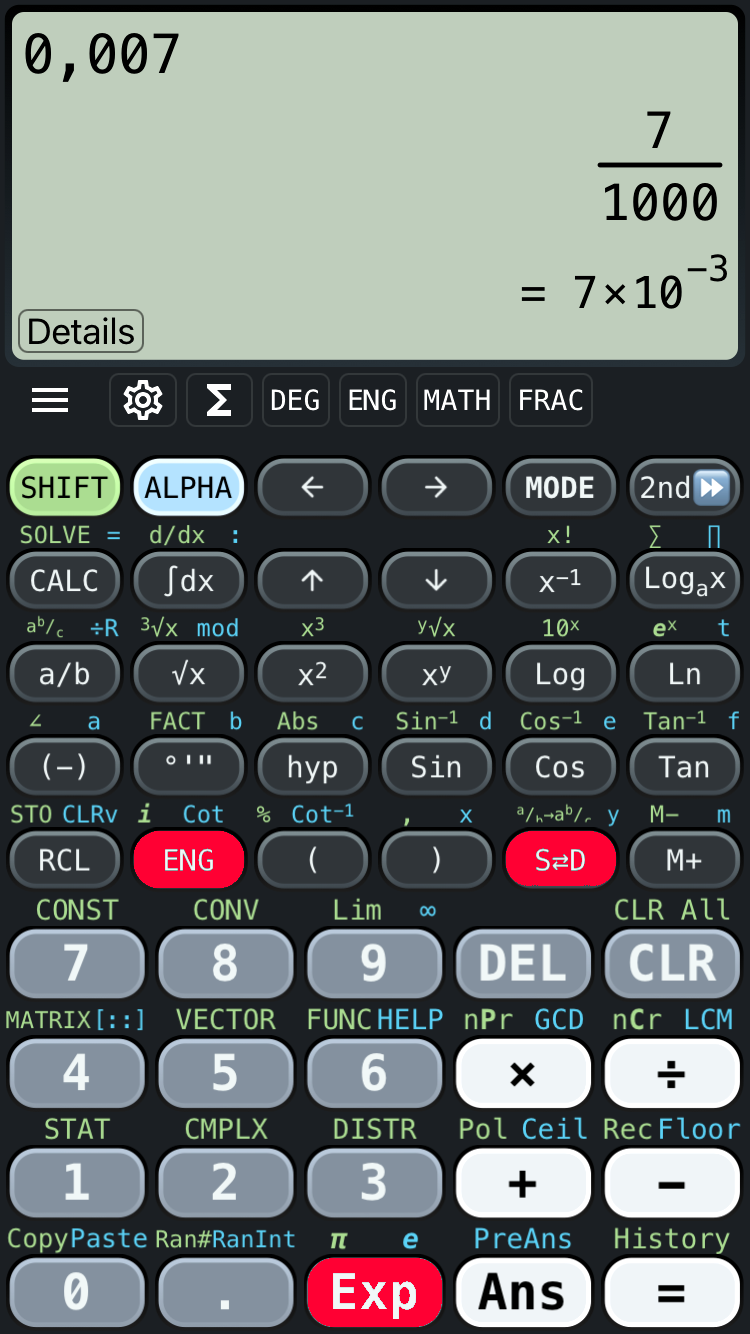
\includegraphics[width=0.85\textwidth]{foto/172}
    \caption{\scriptsize Verschiedene Darstellungen der Zahl 0,007 in einer Taschenrechner-App}
    \label{e_taschenrechner}
\end{figure}

   \end{column}
\end{columns}

\end{frame}

\begin{frame}
\only<1>{
\begin{QQuestion}{EA108}{\qty{0,00042}{\A} entspricht~...}{$420\cdot 10^6$ A.}
{$420\cdot 10^{-6}$ A.}
{$420\cdot 10^{-5}$ A.}
{$42\cdot 10^{-6}$ A.}
\end{QQuestion}

}
\only<2>{
\begin{QQuestion}{EA108}{\qty{0,00042}{\A} entspricht~...}{$420\cdot 10^6$ A.}
{\textbf{\textcolor{DARCgreen}{$420\cdot 10^{-6}$ A.}}}
{$420\cdot 10^{-5}$ A.}
{$42\cdot 10^{-6}$ A.}
\end{QQuestion}

}
\end{frame}

\begin{frame}
\only<1>{
\begin{QQuestion}{EA109}{\qty{0,042}{\A} entspricht~...}{$42\cdot 10^{-1}$ A.}
{$42\cdot 10^3$ A.}
{$42\cdot 10^{-2}$ A.}
{$42\cdot 10^{-3}$ A.}
\end{QQuestion}

}
\only<2>{
\begin{QQuestion}{EA109}{\qty{0,042}{\A} entspricht~...}{$42\cdot 10^{-1}$ A.}
{$42\cdot 10^3$ A.}
{$42\cdot 10^{-2}$ A.}
{\textbf{\textcolor{DARCgreen}{$42\cdot 10^{-3}$ A.}}}
\end{QQuestion}

}
\end{frame}

\begin{frame}
\only<1>{
\begin{QQuestion}{EA110}{\qty{4200000}{\Hz} entspricht~...}{$4,2\cdot 10^5$ Hz.}
{$4,2\cdot 10^6$ Hz.}
{$42\cdot 10^6$ Hz.}
{$42\cdot 10^{-5}$ Hz.}
\end{QQuestion}

}
\only<2>{
\begin{QQuestion}{EA110}{\qty{4200000}{\Hz} entspricht~...}{$4,2\cdot 10^5$ Hz.}
{\textbf{\textcolor{DARCgreen}{$4,2\cdot 10^6$ Hz.}}}
{$42\cdot 10^6$ Hz.}
{$42\cdot 10^{-5}$ Hz.}
\end{QQuestion}

}
\end{frame}

\begin{frame}
\only<1>{
\begin{QQuestion}{EA111}{\qty{0,01}{\mV} entspricht~...}{$1\cdot 10^{-7}$ V.}
{$10\cdot 10^{-6}$ V.}
{$10\cdot 10^{-5}$ V.}
{$0{,}01\cdot 10^{3}$ V.}
\end{QQuestion}

}
\only<2>{
\begin{QQuestion}{EA111}{\qty{0,01}{\mV} entspricht~...}{$1\cdot 10^{-7}$ V.}
{\textbf{\textcolor{DARCgreen}{$10\cdot 10^{-6}$ V.}}}
{$10\cdot 10^{-5}$ V.}
{$0{,}01\cdot 10^{3}$ V.}
\end{QQuestion}

}
\end{frame}

\begin{frame}
\only<1>{
\begin{QQuestion}{EA112}{\qty{0,002}{\Mohm} entspricht~...}{$20\cdot 10^{3} \Omega$.}
{$2\cdot 10^{3} \Omega$.}
{$2\cdot 10^{2} \Omega$.}
{$2000\cdot 10^{2} \Omega$.}
\end{QQuestion}

}
\only<2>{
\begin{QQuestion}{EA112}{\qty{0,002}{\Mohm} entspricht~...}{$20\cdot 10^{3} \Omega$.}
{\textbf{\textcolor{DARCgreen}{$2\cdot 10^{3} \Omega$.}}}
{$2\cdot 10^{2} \Omega$.}
{$2000\cdot 10^{2} \Omega$.}
\end{QQuestion}

}
\end{frame}

\begin{frame}
\only<1>{
\begin{QQuestion}{EA113}{$2\cdot 10^{-7}$ W entspricht~...}{\qty{20}{\micro\W}.}
{\qty{2}{\micro\W}.}
{\qty{0,2}{\micro\W}.}
{\qty{200}{\micro\W}.}
\end{QQuestion}

}
\only<2>{
\begin{QQuestion}{EA113}{$2\cdot 10^{-7}$ W entspricht~...}{\qty{20}{\micro\W}.}
{\qty{2}{\micro\W}.}
{\textbf{\textcolor{DARCgreen}{\qty{0,2}{\micro\W}.}}}
{\qty{200}{\micro\W}.}
\end{QQuestion}

}
\end{frame}

\begin{frame}
\only<1>{
\begin{QQuestion}{EA114}{$5 \cdot 10^{-1}$ W entspricht~...}{\qty{500}{\mW}.}
{\qty{5}{\W}.}
{\qty{-500}{\mW}.}
{\qty{-5}{\W}.}
\end{QQuestion}

}
\only<2>{
\begin{QQuestion}{EA114}{$5 \cdot 10^{-1}$ W entspricht~...}{\textbf{\textcolor{DARCgreen}{\qty{500}{\mW}.}}}
{\qty{5}{\W}.}
{\qty{-500}{\mW}.}
{\qty{-5}{\W}.}
\end{QQuestion}

}
\end{frame}

\begin{frame}
\only<1>{
\begin{QQuestion}{EA115}{0,22~μF entspricht~...}{\qty{22}{\pF}.}
{\qty{22}{\nF}.}
{\qty{220}{\pF}.}
{\qty{220}{\nF}.}
\end{QQuestion}

}
\only<2>{
\begin{QQuestion}{EA115}{0,22~μF entspricht~...}{\qty{22}{\pF}.}
{\qty{22}{\nF}.}
{\qty{220}{\pF}.}
{\textbf{\textcolor{DARCgreen}{\qty{220}{\nF}.}}}
\end{QQuestion}

}
\end{frame}

\begin{frame}
\only<1>{
\begin{QQuestion}{EA116}{\qty{3750}{\kHz} entspricht~...}{\qty{37500000}{\Hz}.}
{\qty{3,750}{\MHz}.}
{\qty{0,03750}{\GHz}.}
{\qty{0,3750}{\GHz}.}
\end{QQuestion}

}
\only<2>{
\begin{QQuestion}{EA116}{\qty{3750}{\kHz} entspricht~...}{\qty{37500000}{\Hz}.}
{\textbf{\textcolor{DARCgreen}{\qty{3,750}{\MHz}.}}}
{\qty{0,03750}{\GHz}.}
{\qty{0,3750}{\GHz}.}
\end{QQuestion}

}
\end{frame}%ENDCONTENT


\section{Formeln umstellen I}
\label{section:formeln_umstellen}
\begin{frame}%STARTCONTENT
Wir hatten bereits

$ U = R\cdot I $

Doch wie kommt man zu

$ R = \dfrac{U}{I} $

und

$ I = \dfrac{U}{R} $

?

\end{frame}

\begin{frame}
\frametitle{Mathematischer Ansatz}
$ U = R\cdot I $ soll nach $ I $ umgestellt werden.

Division auf beiden Seiten durch die Größe, die man auf der Seite mit dem Ziel \enquote{weg} haben möchte.
    \pause
    Division durch  $ R $: $\enspace \dfrac{U}{R} = \dfrac{\cancel{R}\cdot I}{\cancel{R}} \xRightarrow{kürzen} \dfrac{U}{R} = I $
    \pause
    Die Seiten dürfen getauscht werden:

$\dfrac{U}{R} = I \rArr I = \dfrac{U}{R} $



\end{frame}

\begin{frame}
\frametitle{Formeln kombinieren}
Wir kennen bereits

$ U = R\cdot I $ und $ P = U\cdot I $
    \pause
    Wenn jedoch $U$ nicht bekannt ist, dafür aber $R$ und $I$, reicht dieses zur Berechnung von $P$:

$ P = U\cdot I \xRightarrow{U einsetzen} P = R\cdot I\cdot I $

$ \rArr P = R\cdot I^2 $



\end{frame}%ENDCONTENT


\section{Wellenlänge II}
\label{section:wellenlaenge_2}
\begin{frame}%STARTCONTENT
\begin{itemize}
  \item Die Wellenlänge $\lambda$ im Freiraum steht zur Frequenz $f$ in Relation mit der Lichtgeschwindigkeit $c_0$
  \item Freiraum bedeuted: Vakuum, Luft
  \item Lichtgeschwindigkeit $c_0 = 299.792.458 \frac{m}{s}$
  \item Im Amateurfunk rechnen wir mit $c = 3\cdot 10^8 \frac{m}{s}$
  \end{itemize}
$c = f\cdot \lambda \quad f = \dfrac{c}{\lambda} \quad \lambda = \dfrac{c}{f}$

\end{frame}

\begin{frame}
\frametitle{Vereinfachung}
$f = \dfrac{c}{\lambda} \quad \lambda = \dfrac{c}{f}$

$f \lbrack MHz\rbrack \approx \dfrac{300}{\lambda \lbrack m\rbrack} \quad \lambda \lbrack m\rbrack \approx \dfrac{300}{f \lbrack MHz\rbrack}$

\end{frame}

\begin{frame}
\only<1>{
\begin{QQuestion}{EB311}{Welcher Wellenlänge $\lambda$ entspricht in etwa die Frequenz \qty{1,84}{\MHz} im Freiraum?}{\qty{61,3}{\m}}
{\qty{6,13}{\m}}
{\qty{316}{\m}}
{\qty{163}{\m}}
\end{QQuestion}

}
\only<2>{
\begin{QQuestion}{EB311}{Welcher Wellenlänge $\lambda$ entspricht in etwa die Frequenz \qty{1,84}{\MHz} im Freiraum?}{\qty{61,3}{\m}}
{\qty{6,13}{\m}}
{\qty{316}{\m}}
{\textbf{\textcolor{DARCgreen}{\qty{163}{\m}}}}
\end{QQuestion}

}
\end{frame}

\begin{frame}
\only<1>{
\begin{QQuestion}{EB312}{Welcher Wellenlänge $\lambda$ entspricht in etwa die Frequenz $f$ = \qty{21}{\MHz}?}{\qty{14,29}{\m}}
{\qty{7,15}{\m}}
{\qty{12,86}{\m}}
{\qty{6,43}{\m}}
\end{QQuestion}

}
\only<2>{
\begin{QQuestion}{EB312}{Welcher Wellenlänge $\lambda$ entspricht in etwa die Frequenz $f$ = \qty{21}{\MHz}?}{\textbf{\textcolor{DARCgreen}{\qty{14,29}{\m}}}}
{\qty{7,15}{\m}}
{\qty{12,86}{\m}}
{\qty{6,43}{\m}}
\end{QQuestion}

}
\end{frame}

\begin{frame}
\only<1>{
\begin{QQuestion}{EB313}{Welcher Wellenlänge $\lambda$ entspricht in etwa die Frequenz \qty{28,5}{\MHz} im Freiraum? }{\qty{10,5}{\m}}
{\qty{15,0}{\m}}
{\qty{9,49}{\m}}
{\qty{9,49}{\cm}}
\end{QQuestion}

}
\only<2>{
\begin{QQuestion}{EB313}{Welcher Wellenlänge $\lambda$ entspricht in etwa die Frequenz \qty{28,5}{\MHz} im Freiraum? }{\textbf{\textcolor{DARCgreen}{\qty{10,5}{\m}}}}
{\qty{15,0}{\m}}
{\qty{9,49}{\m}}
{\qty{9,49}{\cm}}
\end{QQuestion}

}
\end{frame}

\begin{frame}
\only<1>{
\begin{QQuestion}{EB314}{Welcher Frequenz $f$ entspricht in etwa eine Wellenlänge von \qty{80,0}{\m} im Freiraum?}{\qty{3,65}{\MHz}}
{\qty{3,75}{\MHz}}
{\qty{3,56}{\MHz}}
{\qty{3,57}{\MHz}}
\end{QQuestion}

}
\only<2>{
\begin{QQuestion}{EB314}{Welcher Frequenz $f$ entspricht in etwa eine Wellenlänge von \qty{80,0}{\m} im Freiraum?}{\qty{3,65}{\MHz}}
{\textbf{\textcolor{DARCgreen}{\qty{3,75}{\MHz}}}}
{\qty{3,56}{\MHz}}
{\qty{3,57}{\MHz}}
\end{QQuestion}

}
\end{frame}

\begin{frame}
\only<1>{
\begin{QQuestion}{EB315}{Welche Frequenz entspricht in etwa einer Wellenlänge $\lambda$ von \qty{30}{\mm} im Freiraum?}{\qty{10}{\GHz}}
{\qty{100}{\GHz}}
{\qty{100}{\MHz}}
{\qty{1}{\GHz}}
\end{QQuestion}

}
\only<2>{
\begin{QQuestion}{EB315}{Welche Frequenz entspricht in etwa einer Wellenlänge $\lambda$ von \qty{30}{\mm} im Freiraum?}{\textbf{\textcolor{DARCgreen}{\qty{10}{\GHz}}}}
{\qty{100}{\GHz}}
{\qty{100}{\MHz}}
{\qty{1}{\GHz}}
\end{QQuestion}

}
\end{frame}

\begin{frame}
\only<1>{
\begin{QQuestion}{EB316}{Eine Wellenlänge $\lambda$ von \qty{10}{\cm} im Freiraum entspricht in etwa einer Frequenz von~...}{\qty{3}{\MHz}.}
{\qty{1}{\GHz}.}
{\qty{3}{\GHz}.}
{\qty{10}{\GHz}.}
\end{QQuestion}

}
\only<2>{
\begin{QQuestion}{EB316}{Eine Wellenlänge $\lambda$ von \qty{10}{\cm} im Freiraum entspricht in etwa einer Frequenz von~...}{\qty{3}{\MHz}.}
{\qty{1}{\GHz}.}
{\textbf{\textcolor{DARCgreen}{\qty{3}{\GHz}.}}}
{\qty{10}{\GHz}.}
\end{QQuestion}

}
\end{frame}%ENDCONTENT


\title{DARC Amateurfunklehrgang Klasse E}
\author{Wellenausbreitung}
\institute{Deutscher Amateur Radio Club e.\,V.}
\begin{frame}
\maketitle
\end{frame}

\section{Troposphäre II}
\label{section:troposphaere_2}
\begin{frame}%STARTCONTENT

\frametitle{Begriffe}
Im folgenden Kapitel werden mehrere Begriffe verwendet, die vorab erklärt werden

\begin{itemize}
  \item \emph{Beugung}: Wellen werden an einem Hindernis abgelenkt
  \item \emph{Streuung}: Ablenkung der Wellen durch Interaktion von Teilchen
  \item \emph{Reflexion}: Gleichgerichtete Streuung
  \item \emph{Brechung} oder \emph{Refraktion}: Ablenkung der Wellen durch Änderung der Ausbreitungsgeschwindigkeit durch ein anderes Medium mit anderer Dichte
  \end{itemize}
\end{frame}

\begin{frame}
\begin{columns}
    \begin{column}{0.48\textwidth}
    \begin{itemize}
  \item Bereits bekannt: Die für den Amateurfunk relevanten Schichten in der Atmosphäre
  \item In der Troposphäre finden Erscheinungen des Wetters statt
  \end{itemize}

    \end{column}
   \begin{column}{0.48\textwidth}
       
\begin{figure}
    \DARCimage{0.85\linewidth}{731include}
    \caption{\scriptsize Für den Amateurfunk relevante Schichten in der Atmosphäre}
    \label{e_atmosphaeren_schichten}
\end{figure}


   \end{column}
\end{columns}

\end{frame}

\begin{frame}
\frametitle{DX in VHF/UHF}
\begin{columns}
    \begin{column}{0.48\textwidth}
    \begin{itemize}
  \item Überhorizontverbindungen bei VHF/UHF entstehen durch Beugung, Reflexion und Streuung in der Troposphäre
  \item Bereiche mit unterschiedlicher Temperatur und Dichte
  \end{itemize}

    \end{column}
   \begin{column}{0.48\textwidth}
       
\begin{figure}
    \DARCimage{0.85\linewidth}{734include}
    \caption{\scriptsize Troposphärische Ausbreitung an verschiedenen Luftschichten}
    \label{e_tropo}
\end{figure}


   \end{column}
\end{columns}

\end{frame}

\begin{frame}
\only<1>{
\begin{QQuestion}{EH301}{Was ist die \glqq Troposphäre\grqq{}? Die Troposphäre ist der Teil der Atmosphäre,~...}{in welchem Aurora-Erscheinungen auftreten können.}
{der sich über den Tropen befindet.}
{in dem es zur Bildung sporadischer E-Regionen kommen kann.}
{in der die Erscheinungen des Wetters stattfinden.}
\end{QQuestion}

}
\only<2>{
\begin{QQuestion}{EH301}{Was ist die \glqq Troposphäre\grqq{}? Die Troposphäre ist der Teil der Atmosphäre,~...}{in welchem Aurora-Erscheinungen auftreten können.}
{der sich über den Tropen befindet.}
{in dem es zur Bildung sporadischer E-Regionen kommen kann.}
{\textbf{\textcolor{DARCgreen}{in der die Erscheinungen des Wetters stattfinden.}}}
\end{QQuestion}

}
\end{frame}

\begin{frame}
\only<1>{
\begin{QQuestion}{EH302}{Überhorizontverbindungen im VHF/UHF-Bereich kommen u.~a. zustande durch~...}{Polarisationsdrehungen in der Troposphäre bei hoch liegender Bewölkung.}
{Beugung, Reflexion und Streuung der Wellen in der Troposphäre durch das Auftreten sporadischer D-Regionen.}
{Beugung, Reflexion und Streuung der Wellen an troposphärischen Bereichen unterschiedlicher Temperatur und Dichte.}
{Polarisationsdrehungen in der Troposphäre an Gewitterfronten.}
\end{QQuestion}

}
\only<2>{
\begin{QQuestion}{EH302}{Überhorizontverbindungen im VHF/UHF-Bereich kommen u.~a. zustande durch~...}{Polarisationsdrehungen in der Troposphäre bei hoch liegender Bewölkung.}
{Beugung, Reflexion und Streuung der Wellen in der Troposphäre durch das Auftreten sporadischer D-Regionen.}
{\textbf{\textcolor{DARCgreen}{Beugung, Reflexion und Streuung der Wellen an troposphärischen Bereichen unterschiedlicher Temperatur und Dichte.}}}
{Polarisationsdrehungen in der Troposphäre an Gewitterfronten.}
\end{QQuestion}

}
\end{frame}

\begin{frame}
\only<1>{
\begin{QQuestion}{EH303}{Für VHF-Weitverkehrsverbindungen wird hauptsächlich die~...}{ionosphärische Ausbreitung genutzt.}
{troposphärische Ausbreitung genutzt.}
{Bodenwellenausbreitung genutzt.}
{Oberflächenwellenausbreitung genutzt.}
\end{QQuestion}

}
\only<2>{
\begin{QQuestion}{EH303}{Für VHF-Weitverkehrsverbindungen wird hauptsächlich die~...}{ionosphärische Ausbreitung genutzt.}
{\textbf{\textcolor{DARCgreen}{troposphärische Ausbreitung genutzt.}}}
{Bodenwellenausbreitung genutzt.}
{Oberflächenwellenausbreitung genutzt.}
\end{QQuestion}

}
\end{frame}%ENDCONTENT


\section{Aurora I}
\label{section:aurora_1}
\begin{frame}%STARTCONTENT

\begin{figure}
    \includegraphics[width=0.85\textwidth]{foto/217}
    \caption{\scriptsize Aurora am Notfunk Ausbildungswochenende im Mai 2024}
    \label{e_aurora}
\end{figure}
\end{frame}

\begin{frame}\begin{itemize}
  \item Aurora- oder Polarlichterscheinung in ca. \qtyrange{90}{200}{\kilo\metre} Höhe
  \item Hauptsächlich über magnetischen Nord- und Südpol
  \item Sauerstoff- und Stickstoffatome werden vom Sonnenwind angeregt oder ionisiert
  \item Sonnenwind: Elektrisch geladene Teilchen
  \item Bei Sonneneruptionen besonders stark
  \end{itemize}
\end{frame}

\begin{frame}
\frametitle{Aurora und Amateurfunk}
\begin{itemize}
  \item Funkwellen können sich an ionisierten Sauerstoff- und Stickstoffatomen brechen
  \item Insbesondere für VHF-DX-Verbindungen nutzbar
  \item Sprache nur schlecht nutzbar (große Bandbreite)
  \item Für CW und Digimodes brauchbar
  \item Rapport: für T wird \enquote{A} vergeben, da Ton rau und schwankend ist 
  \end{itemize}
\end{frame}

\begin{frame}
\only<1>{
\begin{QQuestion}{EH305}{Wie wird ein Aurora-Signal in Morsetelegrafie beurteilt?}{Es wird beurteilt mit R und T, weil die Signalstärke stark schwankt.}
{Es wird beurteilt mit R, S und T, da Aurora-Verbindungen überwiegend in CW getätigt werden.}
{Es wird beurteilt mit R, S und \glqq A\grqq{} für Aurora, da der Ton bei Aurora sehr rau ist und nicht beurteilt werden kann.}
{Es wird beurteilt mit R, S, T und \glqq A\grqq{} für Aurora.}
\end{QQuestion}

}
\only<2>{
\begin{QQuestion}{EH305}{Wie wird ein Aurora-Signal in Morsetelegrafie beurteilt?}{Es wird beurteilt mit R und T, weil die Signalstärke stark schwankt.}
{Es wird beurteilt mit R, S und T, da Aurora-Verbindungen überwiegend in CW getätigt werden.}
{\textbf{\textcolor{DARCgreen}{Es wird beurteilt mit R, S und \glqq A\grqq{} für Aurora, da der Ton bei Aurora sehr rau ist und nicht beurteilt werden kann.}}}
{Es wird beurteilt mit R, S, T und \glqq A\grqq{} für Aurora.}
\end{QQuestion}

}
\end{frame}%ENDCONTENT


\section{Sporadic-E II}
\label{section:sporadic_e_2}
\begin{frame}%STARTCONTENT

\begin{columns}
    \begin{column}{0.48\textwidth}
    \begin{itemize}
  \item Regional begrenzte ungewöhnlich hohe Ionisation der E-Schicht
  \item Refraktion (Brechung) von Funkwellen in VHF und UHF
  \item Auch \qty{10}{\metre}-Band möglich
  \end{itemize}

    \end{column}
   \begin{column}{0.48\textwidth}
       
\begin{figure}
    \DARCimage{0.85\linewidth}{731include}
    \caption{\scriptsize Für den Amateurfunk relevante Schichten in der Atmosphäre}
    \label{e_atmosphaeren_schichten}
\end{figure}


   \end{column}
\end{columns}

\end{frame}

\begin{frame}
\only<1>{
\begin{QQuestion}{EH304}{Was verstehen Sie unter dem Begriff \glqq Sporadic-E\grqq{}?}{Kurzzeitig auftretende starke Reflexion von VHF-Signalen an Meteorbahnen innerhalb der E-Region.}
{Kurzfristige plötzliche Inversionsänderungen in der E-Region, die Fernausbreitung im VHF-Bereich ermöglichen.}
{Die Refraktion (Brechung) in lokal begrenzten Bereichen mit ungewöhnlich hoher Ionisation innerhalb der E-Region.}
{Lokal begrenzten kurzzeitigen Ausfall der Reflexion durch ungewöhnlich hohe Ionisation innerhalb der E-Region.}
\end{QQuestion}

}
\only<2>{
\begin{QQuestion}{EH304}{Was verstehen Sie unter dem Begriff \glqq Sporadic-E\grqq{}?}{Kurzzeitig auftretende starke Reflexion von VHF-Signalen an Meteorbahnen innerhalb der E-Region.}
{Kurzfristige plötzliche Inversionsänderungen in der E-Region, die Fernausbreitung im VHF-Bereich ermöglichen.}
{\textbf{\textcolor{DARCgreen}{Die Refraktion (Brechung) in lokal begrenzten Bereichen mit ungewöhnlich hoher Ionisation innerhalb der E-Region.}}}
{Lokal begrenzten kurzzeitigen Ausfall der Reflexion durch ungewöhnlich hohe Ionisation innerhalb der E-Region.}
\end{QQuestion}

}
\end{frame}

\begin{frame}
\frametitle{Short Skip}
\begin{columns}
    \begin{column}{0.48\textwidth}
    \begin{itemize}
  \item Funkverbindungen mit Sprungentfernungen unter \qty{1000}{\kilo\metre}
  \item Durch Refraktion an einer Sporadic-E-Schicht
  \item Insbesondere im \qty{10}{\metre}-Band
  \end{itemize}

    \end{column}
   \begin{column}{0.48\textwidth}
       
\begin{figure}
    \DARCimage{0.85\linewidth}{733include}
    \caption{\scriptsize Refraktion bei Sporadic-E}
    \label{e_sporadic_e}
\end{figure}


   \end{column}
\end{columns}

\end{frame}

\begin{frame}
\only<1>{
\begin{QQuestion}{EH218}{Unter dem Begriff \glqq Short Skip\grqq{} versteht man Funkverbindungen besonders im \qty{10}{\m}-Band mit Sprungentfernungen unter \qty{1000}{\km}, die~...}{durch Refraktion (Brechung) in sporadischen E-Regionen ermöglicht werden.}
{bei entsprechendem Abstrahlwinkel durch Refraktion (Brechung) in der F1-Region ermöglicht werden.}
{bei entsprechendem Abstrahlwinkel durch Refraktion (Brechung) in der F2-Region ermöglicht werden.}
{durch Refraktion (Brechung) in der hochionisierten D-Region ermöglicht werden.}
\end{QQuestion}

}
\only<2>{
\begin{QQuestion}{EH218}{Unter dem Begriff \glqq Short Skip\grqq{} versteht man Funkverbindungen besonders im \qty{10}{\m}-Band mit Sprungentfernungen unter \qty{1000}{\km}, die~...}{\textbf{\textcolor{DARCgreen}{durch Refraktion (Brechung) in sporadischen E-Regionen ermöglicht werden.}}}
{bei entsprechendem Abstrahlwinkel durch Refraktion (Brechung) in der F1-Region ermöglicht werden.}
{bei entsprechendem Abstrahlwinkel durch Refraktion (Brechung) in der F2-Region ermöglicht werden.}
{durch Refraktion (Brechung) in der hochionisierten D-Region ermöglicht werden.}
\end{QQuestion}

}
\end{frame}%ENDCONTENT


\section{Ionosphäre II}
\label{section:ionosphaere_2}
\begin{frame}%STARTCONTENT

\begin{columns}
    \begin{column}{0.48\textwidth}
    \begin{itemize}
  \item Ionosphäre enthält große Menge von Ionen und freier Elektronen
  \item In ca. \qtyrange{50}{450}{\kilo\metre} Höhe
  \item Refraktion von Kurzwellen, wodurch weltweite Kommunikation ermöglicht wird
  \end{itemize}

    \end{column}
   \begin{column}{0.48\textwidth}
       
\begin{figure}
    \DARCimage{0.85\linewidth}{731include}
    \caption{\scriptsize Für den Amateurfunk relevante Schichten in der Atmosphäre}
    \label{e_atmosphaeren_schichten}
\end{figure}


   \end{column}
\end{columns}

\end{frame}

\begin{frame}
\only<1>{
\begin{QQuestion}{EH101}{Wie kommt die Fernausbreitung einer Funkwelle auf den Kurzwellenbändern zustande? Sie kommt zustande durch die Refraktion (Brechung) an~...}{den Wolken in der niedrigen Atmosphäre.}
{Hoch- und Tiefdruckgebieten der hohen Atmosphäre.}
{elektrisch aufgeladenen Luftschichten in der Ionosphäre.}
{den parasitären Elementen einer Richtantenne.}
\end{QQuestion}

}
\only<2>{
\begin{QQuestion}{EH101}{Wie kommt die Fernausbreitung einer Funkwelle auf den Kurzwellenbändern zustande? Sie kommt zustande durch die Refraktion (Brechung) an~...}{den Wolken in der niedrigen Atmosphäre.}
{Hoch- und Tiefdruckgebieten der hohen Atmosphäre.}
{\textbf{\textcolor{DARCgreen}{elektrisch aufgeladenen Luftschichten in der Ionosphäre.}}}
{den parasitären Elementen einer Richtantenne.}
\end{QQuestion}

}
\end{frame}

\begin{frame}
\frametitle{Ausbreitung von Funkwellen}
\begin{columns}
    \begin{column}{0.48\textwidth}
    \begin{itemize}
  \item In den kommenden Abschnitten werden Einflüsse der Funkwellenausbreitung an der Ionosphäre besprochen
  \item Und mit welchen Maßnahmen wir die Ausbreitung unserer Funkwellen optimieren können
  \item Zuerst eine exemplarische Betrachtung der Wellenausbreitung
  \end{itemize}

    \end{column}
   \begin{column}{0.48\textwidth}
       
\begin{figure}
    \DARCimage{0.85\linewidth}{865include}
    \caption{\scriptsize Refraktion an Schichten der Ionosphäre}
    \label{e_wellenausbreitung_refraktion}
\end{figure}


   \end{column}
\end{columns}

\end{frame}

\begin{frame}\end{frame}

\begin{frame}
\frametitle{Schichten der Ionosphäre}
\begin{itemize}
  \item Es gibt in verschiedenen Höhen verschiedene \enquote{Schichten} bzw. Regionen mit unterschiedlich starker Ionisierung
  \item Diese tragen die Namen
  \end{itemize}
\begin{enumerate}
  \item[1] D-Schicht
  \item[2] E-Schicht
  \item[3] F<sub>1</sub>-Schicht
  \item[4] F<sub>2</sub>-Schicht
  \end{enumerate}
\end{frame}

\begin{frame}
\frametitle{D-Region}
\begin{itemize}
  \item In ca. 50–\qty{90}{\kilo\metre} Höhe
  \item Existiert \emph{nur am Tag}
  \item Nach Sonnenuntergang sehr schnell verschwunden
  \item Starke \emph{Dämpfung} von Funkwellen unter \qty{10}{\mega\hertz}
  \item Keine Raumwelle für Amateurfunkbänder wie \qty{160}{\metre} oder 80m
  \end{itemize}

\end{frame}

\begin{frame}
\only<1>{
\begin{QQuestion}{EH210}{Warum sind Signale im 160- und \qty{80}{\m}-Band tagsüber nur schwach und nicht für den weltweiten Funkverkehr geeignet? Sie sind ungeeignet wegen der Tagesdämpfung in der~...}{A-Region.}
{F1-Region.}
{F2-Region.}
{D-Region.}
\end{QQuestion}

}
\only<2>{
\begin{QQuestion}{EH210}{Warum sind Signale im 160- und \qty{80}{\m}-Band tagsüber nur schwach und nicht für den weltweiten Funkverkehr geeignet? Sie sind ungeeignet wegen der Tagesdämpfung in der~...}{A-Region.}
{F1-Region.}
{F2-Region.}
{\textbf{\textcolor{DARCgreen}{D-Region.}}}
\end{QQuestion}

}
\end{frame}

\begin{frame}
\only<1>{
\begin{QQuestion}{EH105}{Welchen Einfluss hat die D-Region auf die Fernausbreitung?}{Die D-Region absorbiert tagsüber die Wellen im \qty{10}{\m}-Band.}
{Die D-Region reflektiert tagsüber die Wellen im 80- und \qty{160}{\m}-Band.}
{Die D-Region führt tagsüber zu starker Dämpfung im 80- und \qty{160}{\m}-Band.}
{Die D-Region verhindert nachts die Fernausbreitung im Lang-, Mittel- und unteren Kurzwellenbereich.}
\end{QQuestion}

}
\only<2>{
\begin{QQuestion}{EH105}{Welchen Einfluss hat die D-Region auf die Fernausbreitung?}{Die D-Region absorbiert tagsüber die Wellen im \qty{10}{\m}-Band.}
{Die D-Region reflektiert tagsüber die Wellen im 80- und \qty{160}{\m}-Band.}
{\textbf{\textcolor{DARCgreen}{Die D-Region führt tagsüber zu starker Dämpfung im 80- und \qty{160}{\m}-Band.}}}
{Die D-Region verhindert nachts die Fernausbreitung im Lang-, Mittel- und unteren Kurzwellenbereich.}
\end{QQuestion}

}
\end{frame}

\begin{frame}
\frametitle{E-Region}
\begin{itemize}
  \item In ca. 90–\qty{130}{\kilo\metre} Höhe
  \item Entsteht \emph{tagsüber} mit Maximum zur Mittagszeit
  \item Verschwindet etwa 1 Stunde nach Sonnenuntergang
  \item Starke Ionisation $\rightarrow$ Sporadic-E
  \item Namensgebene: \emph{E}(lektrische)\emph{-Schicht}
  \end{itemize}

\end{frame}

\begin{frame}
\only<1>{
\begin{QQuestion}{EH106}{Welche ionosphärische Region sorgt während der Sommermonate für gelegentliche gute Ausbreitung vom oberen Kurzwellenbereich bis in den UKW-Bereich?}{Die E-Region}
{Die D-Region}
{Die F1-Region}
{Die F2-Region}
\end{QQuestion}

}
\only<2>{
\begin{QQuestion}{EH106}{Welche ionosphärische Region sorgt während der Sommermonate für gelegentliche gute Ausbreitung vom oberen Kurzwellenbereich bis in den UKW-Bereich?}{\textbf{\textcolor{DARCgreen}{Die E-Region}}}
{Die D-Region}
{Die F1-Region}
{Die F2-Region}
\end{QQuestion}

}
\end{frame}

\begin{frame}
\frametitle{F-Regionen}
\begin{itemize}
  \item In ca. 200–\qty{400}{\kilo\metre} Höhe
  \item Am stärksten ionisierte Schicht
  \item F<sub>1</sub>-Schicht existiert \emph{nur am Tag}
  \item F<sub>2</sub>-Schicht bleibt \emph{nachts} bestehen
  \end{itemize}
\end{frame}

\begin{frame}
\only<1>{
\begin{QQuestion}{EH104}{Welche ionosphärische Region ermöglicht DX-Verbindungen im \qty{80}{\m}-Band in der Nacht?}{Die E-Region}
{Die F2-Region}
{Die D-Region}
{Die F1-Region}
\end{QQuestion}

}
\only<2>{
\begin{QQuestion}{EH104}{Welche ionosphärische Region ermöglicht DX-Verbindungen im \qty{80}{\m}-Band in der Nacht?}{Die E-Region}
{\textbf{\textcolor{DARCgreen}{Die F2-Region}}}
{Die D-Region}
{Die F1-Region}
\end{QQuestion}

}
\end{frame}

\begin{frame}
\only<1>{
\begin{QQuestion}{EH103}{Welche ionosphärische Region ermöglicht im wesentlichen Weitverkehrsverbindungen im Kurzwellenbereich?}{D-Region}
{F2-Region}
{E-Region}
{F1-Region}
\end{QQuestion}

}
\only<2>{
\begin{QQuestion}{EH103}{Welche ionosphärische Region ermöglicht im wesentlichen Weitverkehrsverbindungen im Kurzwellenbereich?}{D-Region}
{\textbf{\textcolor{DARCgreen}{F2-Region}}}
{E-Region}
{F1-Region}
\end{QQuestion}

}
\end{frame}

\begin{frame}
\only<1>{
\begin{QQuestion}{EH102}{In welcher Höhe befinden sich für die Kurzwellen-Fernausbreitung (DX) wichtige ionosphärische Regionen? Sie befinden sich in ungefähr~...}{\qtyrange{130}{450}{\km} Höhe.}
{\qtyrange{50}{90}{\km} Höhe.}
{\qtyrange{90}{130}{\km} Höhe.}
{\qtyrange{130}{200}{\km} Höhe.}
\end{QQuestion}

}
\only<2>{
\begin{QQuestion}{EH102}{In welcher Höhe befinden sich für die Kurzwellen-Fernausbreitung (DX) wichtige ionosphärische Regionen? Sie befinden sich in ungefähr~...}{\textbf{\textcolor{DARCgreen}{\qtyrange{130}{450}{\km} Höhe.}}}
{\qtyrange{50}{90}{\km} Höhe.}
{\qtyrange{90}{130}{\km} Höhe.}
{\qtyrange{130}{200}{\km} Höhe.}
\end{QQuestion}

}

\end{frame}

\begin{frame}
\frametitle{Sonnenzyklus}
\begin{columns}
    \begin{column}{0.48\textwidth}
    \begin{itemize}
  \item Im Schnitt alle 11 Jahre durch Umkehrung des Magnetfelds
  \item Führt zu starker Ionisation der F<sub>2</sub>-Region
  \end{itemize}

    \end{column}
   \begin{column}{0.48\textwidth}
       
\begin{figure}
    \DARCimage{0.85\linewidth}{729include}
    \caption{\scriptsize Zählung der monatlichen Sonnenflecken seit 1749}
    \label{e_sonnenzyklus}
\end{figure}


   \end{column}
\end{columns}

\end{frame}

\begin{frame}
\frametitle{Ursachen des Sonnenzyklus}
\begin{itemize}
  \item Polregionen der Sonne rotieren langsamer als Äquator
  \item Führt zu inneren Spannungen des Magnetfelds
  \item Magnetfelder zwischen Sonnenflecken fallen abrupt zusammen $\rightarrow$ Plasma wird freigesetzt und hat Einfluss auf die Ionosphäre der Erde
  \end{itemize}
\end{frame}

\begin{frame}
\only<1>{
\begin{QQuestion}{EH107}{Die Sonnenaktivität ist einem regelmäßigen Zyklus unterworfen. Welchen Zeitraum hat dieser Zyklus ungefähr?}{12 Monate}
{6 Monate}
{11 Jahre}
{7 Jahre}
\end{QQuestion}

}
\only<2>{
\begin{QQuestion}{EH107}{Die Sonnenaktivität ist einem regelmäßigen Zyklus unterworfen. Welchen Zeitraum hat dieser Zyklus ungefähr?}{12 Monate}
{6 Monate}
{\textbf{\textcolor{DARCgreen}{11 Jahre}}}
{7 Jahre}
\end{QQuestion}

}
\end{frame}

\begin{frame}
\only<1>{
\begin{QQuestion}{EH205}{Welche Aussage ist für das Sonnenfleckenmaximum richtig?}{Die Sonnenaktivität ist sehr hoch und führt zu stärkerer Ionisation in der F-Region.}
{Die Sonnenaktivität ist sehr hoch und führt zu schwächerer Ionisation in der F-Region.}
{Die Sonnenaktivität verringert sich stark und führt zu stärkerer Ionisation in der F-Region.}
{Die Sonnenaktivität ist in der Nacht sehr hoch, am Tag sehr schwach und führt deshalb zu keiner Ionisation in der D-Region.}
\end{QQuestion}

}
\only<2>{
\begin{QQuestion}{EH205}{Welche Aussage ist für das Sonnenfleckenmaximum richtig?}{\textbf{\textcolor{DARCgreen}{Die Sonnenaktivität ist sehr hoch und führt zu stärkerer Ionisation in der F-Region.}}}
{Die Sonnenaktivität ist sehr hoch und führt zu schwächerer Ionisation in der F-Region.}
{Die Sonnenaktivität verringert sich stark und führt zu stärkerer Ionisation in der F-Region.}
{Die Sonnenaktivität ist in der Nacht sehr hoch, am Tag sehr schwach und führt deshalb zu keiner Ionisation in der D-Region.}
\end{QQuestion}

}
\end{frame}

\begin{frame}
\only<1>{
\begin{QQuestion}{EH219}{Welches Frequenzband kann im Sonnenfleckenmaximum tagsüber auch mit kleiner Leistung für weltweite Funkverbindungen verwendet werden?}{\qty{10}{\m}-Band}
{\qty{2}{\m}-Band}
{\qty{80}{\m}-Band}
{\qty{160}{\m}-Band}
\end{QQuestion}

}
\only<2>{
\begin{QQuestion}{EH219}{Welches Frequenzband kann im Sonnenfleckenmaximum tagsüber auch mit kleiner Leistung für weltweite Funkverbindungen verwendet werden?}{\textbf{\textcolor{DARCgreen}{\qty{10}{\m}-Band}}}
{\qty{2}{\m}-Band}
{\qty{80}{\m}-Band}
{\qty{160}{\m}-Band}
\end{QQuestion}

}
\end{frame}%ENDCONTENT


\section{Tote Zone I}
\label{section:tote_zone_1}
\begin{frame}%STARTCONTENT

\begin{columns}
    \begin{column}{0.48\textwidth}
    \begin{itemize}
  \item Bereich, wo die \emph{Bodenwelle nicht mehr} hin gelangt
  \item Und die \emph{Raumwelle noch nicht} hingelangt
  \item Abhängig vom Reflexionswinkel der Raumwelle
  \item Funkstationen in der Toten Zone können mich nicht hören
  \end{itemize}

    \end{column}
   \begin{column}{0.48\textwidth}
       
\begin{figure}
    \DARCimage{0.85\linewidth}{741include}
    \caption{\scriptsize Tote Zone}
    \label{e_tote_zone}
\end{figure}


   \end{column}
\end{columns}

\end{frame}

\begin{frame}
\only<1>{
\begin{QQuestion}{EH201}{Unter der \glqq Toten Zone\grqq{} wird der Bereich verstanden,~...}{der durch die Bodenwelle erreicht wird und für die Raumwelle nicht zugänglich ist.}
{der durch die Bodenwelle überdeckt wird, so dass schwächere DX-Stationen zugedeckt werden.}
{der durch die Bodenwelle nicht mehr erreicht wird und durch die Raumwelle noch nicht erreicht wird.}
{der durch die Überlagerung der Bodenwelle mit der Raumwelle in einer Zone der gegenseitigen Auslöschung liegt.}
\end{QQuestion}

}
\only<2>{
\begin{QQuestion}{EH201}{Unter der \glqq Toten Zone\grqq{} wird der Bereich verstanden,~...}{der durch die Bodenwelle erreicht wird und für die Raumwelle nicht zugänglich ist.}
{der durch die Bodenwelle überdeckt wird, so dass schwächere DX-Stationen zugedeckt werden.}
{\textbf{\textcolor{DARCgreen}{der durch die Bodenwelle nicht mehr erreicht wird und durch die Raumwelle noch nicht erreicht wird.}}}
{der durch die Überlagerung der Bodenwelle mit der Raumwelle in einer Zone der gegenseitigen Auslöschung liegt.}
\end{QQuestion}

}
\end{frame}%ENDCONTENT


\section{Fading}
\label{section:fading}
\begin{frame}%STARTCONTENT

\begin{columns}
    \begin{column}{0.48\textwidth}
    \begin{itemize}
  \item Raumwelle trifft noch im Bereich der Bodenwelle wieder zum Empfänger
  \item Durch Wellenüberlagerung können sich Raum- und Bodenwelle gegenseitig abschwächen
  \item Signal verliert an Stärke $\rightarrow$ \emph{Fading}
  \end{itemize}

    \end{column}
   \begin{column}{0.48\textwidth}
       
   \end{column}
\end{columns}

\end{frame}

\begin{frame}
\only<1>{
\begin{QQuestion}{EH203}{Wie nennt man den Feldstärkeschwund durch Überlagerung von Boden- und Raumwelle?}{Fading}
{Backscatter}
{MUF}
{Mögel-Dellinger-Effekt}
\end{QQuestion}

}
\only<2>{
\begin{QQuestion}{EH203}{Wie nennt man den Feldstärkeschwund durch Überlagerung von Boden- und Raumwelle?}{\textbf{\textcolor{DARCgreen}{Fading}}}
{Backscatter}
{MUF}
{Mögel-Dellinger-Effekt}
\end{QQuestion}

}
\end{frame}

\begin{frame}
\only<1>{
\begin{QQuestion}{EH202}{Was kann durch das Zusammenwirken von Raum- und Bodenwelle verursacht werden?}{Frequenzverschiebung (Doppler-Effekt)}
{Feldstärkeschwankungen (Fading)}
{Rückstreuung (Backscatter)}
{Rauschen (Noise)}
\end{QQuestion}

}
\only<2>{
\begin{QQuestion}{EH202}{Was kann durch das Zusammenwirken von Raum- und Bodenwelle verursacht werden?}{Frequenzverschiebung (Doppler-Effekt)}
{\textbf{\textcolor{DARCgreen}{Feldstärkeschwankungen (Fading)}}}
{Rückstreuung (Backscatter)}
{Rauschen (Noise)}
\end{QQuestion}

}
\end{frame}%ENDCONTENT


\section{Sprungdistanz I}
\label{section:sprungdistanz_1}
\begin{frame}%STARTCONTENT

\begin{columns}
    \begin{column}{0.48\textwidth}
    \begin{itemize}
  \item Je flacher meine Antenne im Winkel zur Erdoberfläche abstrahlt, umso weiter ist die Sprungdistanz
  \item Je steiler meine Antenne nach oben strahlt, umso kürzer ist die Sprungdistanz
  \end{itemize}

    \end{column}
   \begin{column}{0.48\textwidth}
       
\begin{figure}
    \DARCimage{0.85\linewidth}{732include}
    \caption{\scriptsize Ausbreitung von Raum- und Bodenwelle}
    \label{e_raum_und_bodenwelle}
\end{figure}


   \end{column}
\end{columns}

\end{frame}

\begin{frame}
\only<1>{
\begin{QQuestion}{EH208}{Von welchem der genannten Parameter ist die Sprungdistanz abhängig, die ein KW-Signal auf der Erdoberfläche überbrücken kann? Sie ist abhängig~...}{von der Sendeleistung.}
{von der Polarisation der Antenne.}
{vom Abstrahlwinkel der Antenne.}
{vom Antennengewinn.}
\end{QQuestion}

}
\only<2>{
\begin{QQuestion}{EH208}{Von welchem der genannten Parameter ist die Sprungdistanz abhängig, die ein KW-Signal auf der Erdoberfläche überbrücken kann? Sie ist abhängig~...}{von der Sendeleistung.}
{von der Polarisation der Antenne.}
{\textbf{\textcolor{DARCgreen}{vom Abstrahlwinkel der Antenne.}}}
{vom Antennengewinn.}
\end{QQuestion}

}
\end{frame}%ENDCONTENT


\section{MUF und LUF}
\label{section:muf_luf_1}
\begin{frame}%STARTCONTENT

\frametitle{Maximal Usable Frequency (MUF)}
\begin{columns}
    \begin{column}{0.48\textwidth}
    \begin{itemize}
  \item Höchste zwischen zwei Orten verwendbare Frequenz
  \item Ist abhängig vom Abstrahlwinkel der Antenne
  \item Und der kritischen Frequenz der Ionosphäre
  \end{itemize}

    \end{column}
   \begin{column}{0.48\textwidth}
       
\begin{figure}
    \DARCimage{0.85\linewidth}{731include}
    \caption{\scriptsize Für den Amateurfunk relevante Schichten in der Atmosphäre}
    \label{e_atmosphaeren_schichten}
\end{figure}


   \end{column}
\end{columns}

\end{frame}

\begin{frame}
\frametitle{Berechnung der MUF}
$MUF \approx \dfrac{f_c}{sin(\alpha)}$

$\alpha$ ist der Abstrahlwinkel der Antenne zum Boden

$f_c$ ist die kritische Frequenz bei der senkrecht auf die Ionosphäre auftretende Funkstrahlen von den Regionen gebrochen werden $\rightarrow$ bei stärkerer Ionisation einer Region steigt die kritische Frequenz

\end{frame}

\begin{frame}
\only<1>{
\begin{QQuestion}{EH204}{Was bedeutet die \glqq MUF\grqq{} bei der Kurzwellenausbreitung?}{Kritische Grenzfrequenz}
{Niedrigste nutzbare Frequenz}
{Höchste nutzbare Frequenz}
{Mittlere Nutzfrequenz}
\end{QQuestion}

}
\only<2>{
\begin{QQuestion}{EH204}{Was bedeutet die \glqq MUF\grqq{} bei der Kurzwellenausbreitung?}{Kritische Grenzfrequenz}
{Niedrigste nutzbare Frequenz}
{\textbf{\textcolor{DARCgreen}{Höchste nutzbare Frequenz}}}
{Mittlere Nutzfrequenz}
\end{QQuestion}

}
\end{frame}

\begin{frame}
\only<1>{
\begin{QQuestion}{EH207}{Sie führen Funkbetrieb nahe der aktuell höchstmöglichen Frequenz (MUF) durch. Um den Funkbetrieb auf noch höheren Frequenzen fortsetzen zu können, muss die Ionisation der brechenden Region~...}{zunehmen.}
{abnehmen.}
{verschwinden.}
{unverändert bleiben.}
\end{QQuestion}

}
\only<2>{
\begin{QQuestion}{EH207}{Sie führen Funkbetrieb nahe der aktuell höchstmöglichen Frequenz (MUF) durch. Um den Funkbetrieb auf noch höheren Frequenzen fortsetzen zu können, muss die Ionisation der brechenden Region~...}{\textbf{\textcolor{DARCgreen}{zunehmen.}}}
{abnehmen.}
{verschwinden.}
{unverändert bleiben.}
\end{QQuestion}

}
\end{frame}

\begin{frame}
\only<1>{
\begin{QQuestion}{EH206}{Eine stärkere Ionisierung der F2-Region führt zu~...}{einer größeren Durchlässigkeit für die höheren Frequenzen.}
{einer stärkeren Absorption der höheren Frequenzen.}
{einer niedrigeren MUF.}
{einer höheren MUF.}
\end{QQuestion}

}
\only<2>{
\begin{QQuestion}{EH206}{Eine stärkere Ionisierung der F2-Region führt zu~...}{einer größeren Durchlässigkeit für die höheren Frequenzen.}
{einer stärkeren Absorption der höheren Frequenzen.}
{einer niedrigeren MUF.}
{\textbf{\textcolor{DARCgreen}{einer höheren MUF.}}}
\end{QQuestion}

}
\end{frame}

\begin{frame}
\frametitle{Lowest Usable Frequency (LUF)}
\begin{columns}
    \begin{column}{0.48\textwidth}
    \begin{itemize}
  \item Abhängig von der Ionisierung in der D-Schicht
  \item Je weniger Dämpfung in der D-Schicht, umso mehr tiefere Funkwellen können diese Schicht durchdringen und an den höheren Schichten reflektieren
  \end{itemize}

    \end{column}
   \begin{column}{0.48\textwidth}
       
\begin{figure}
    \DARCimage{0.85\linewidth}{731include}
    \caption{\scriptsize Für den Amateurfunk relevante Schichten in der Atmosphäre}
    \label{e_atmosphaeren_schichten}
\end{figure}


   \end{column}
\end{columns}

\end{frame}

\begin{frame}
\only<1>{
\begin{QQuestion}{EH209}{Die niedrigste brauchbare Frequenz (LUF) bei Raumwellenausbreitung zwischen zwei Orten hängt ab~...}{vom Ionisierungsgrad in der E-Region.}
{vom Abstrahlwinkel der Antenne.}
{vom Ionisierungsgrad in der D-Region.}
{von der Polarisation der Antenne.}
\end{QQuestion}

}
\only<2>{
\begin{QQuestion}{EH209}{Die niedrigste brauchbare Frequenz (LUF) bei Raumwellenausbreitung zwischen zwei Orten hängt ab~...}{vom Ionisierungsgrad in der E-Region.}
{vom Abstrahlwinkel der Antenne.}
{\textbf{\textcolor{DARCgreen}{vom Ionisierungsgrad in der D-Region.}}}
{von der Polarisation der Antenne.}
\end{QQuestion}

}
\end{frame}%ENDCONTENT


\section{Bodenwelle}
\label{section:bodenwelle}
\begin{frame}%STARTCONTENT

\begin{columns}
    \begin{column}{0.48\textwidth}
    \begin{itemize}
  \item Die Bodenwelle reicht über den sichtbaren Horizont raus
  \item Folgt der Erdkrümmung
  \item Am besten für Frequenzen unter \qty{3}{\mega\hertz}
  \end{itemize}

    \end{column}
   \begin{column}{0.48\textwidth}
       
\begin{figure}
    \DARCimage{0.85\linewidth}{866include}
    \caption{\scriptsize Reichweite der Bodenwelle je nach Band}
    \label{e_reichweite_bodenwelle}
\end{figure}


   \end{column}
\end{columns}

\end{frame}

\begin{frame}
\frametitle{Reichweite}
\begin{itemize}
  \item Reichweite ist von Frequenz und Bodenbeschaffenheit abhängig
  \item Langwelle (\qty{30}{\kilo\hertz}–\qty{300}{\kilo\hertz}) bis zu \qty{1000}{\kilo\metre}, Mittelwelle (\qty{300}{\kilo\hertz}–\qty{3}{\mega\hertz}) bis zu \qty{250}{\kilo\metre}
  \item Gut nutzbar im \qty{160}{\metre}-Band
  \item Im \qty{10}{\metre}-Band für Kommunikation im Stadtbereich nutzbar
  \item VHF und höhere Frequenzen vernachlässigbar
  \end{itemize}

\end{frame}

\begin{frame}
\only<1>{
\begin{QQuestion}{EH211}{Die Ausbreitung der Wellen im \qty{160}{\m}-Band erfolgt tagsüber hauptsächlich~...}{über die Raumwelle, weil es in der Troposphäre durch Temperaturinversionen zu Reflexionen für die Frequenzen unter \qty{2}{\MHz} kommen kann.}
{über die Raumwelle, weil die Refraktion (Brechung) in der D-Region für Frequenzen bis zu \qty{2}{\MHz} besonders stark ist.}
{über Raum- und Bodenwelle, weil es bei den Frequenzen unter \qty{2}{\MHz} nur zu geringfügiger Phasenverschiebung zwischen reflektierter und direkter Welle kommt.}
{über die Bodenwelle, weil durch die Dämpfung der D-Region keine Raumwelle entstehen kann.}
\end{QQuestion}

}
\only<2>{
\begin{QQuestion}{EH211}{Die Ausbreitung der Wellen im \qty{160}{\m}-Band erfolgt tagsüber hauptsächlich~...}{über die Raumwelle, weil es in der Troposphäre durch Temperaturinversionen zu Reflexionen für die Frequenzen unter \qty{2}{\MHz} kommen kann.}
{über die Raumwelle, weil die Refraktion (Brechung) in der D-Region für Frequenzen bis zu \qty{2}{\MHz} besonders stark ist.}
{über Raum- und Bodenwelle, weil es bei den Frequenzen unter \qty{2}{\MHz} nur zu geringfügiger Phasenverschiebung zwischen reflektierter und direkter Welle kommt.}
{\textbf{\textcolor{DARCgreen}{über die Bodenwelle, weil durch die Dämpfung der D-Region keine Raumwelle entstehen kann.}}}
\end{QQuestion}

}
\end{frame}

\begin{frame}
\only<1>{
\begin{QQuestion}{EH212}{Welche der folgenden Aussagen trifft für KW-Funkverbindungen zu, die über Bodenwellen erfolgen?}{Die Bodenwelle folgt der Erdkrümmung und geht nicht über den geografischen Horizont hinaus. Sie wird in niedrigeren Frequenzbereichen stärker gedämpft als in höheren Frequenzbereichen.}
{Die Bodenwelle folgt der Erdkrümmung und geht nicht über den geografischen Horizont hinaus. Sie wird in höheren Frequenzbereichen stärker gedämpft als in niedrigeren Frequenzbereichen.}
{Die Bodenwelle folgt der Erdkrümmung und geht über den geografischen Horizont hinaus. Sie wird in niedrigeren Frequenzbereichen stärker gedämpft als in höheren Frequenzbereichen.}
{Die Bodenwelle folgt der Erdkrümmung und geht über den geografischen Horizont hinaus. Sie wird in höheren Frequenzbereichen stärker gedämpft als in niedrigeren Frequenzbereichen.}
\end{QQuestion}

}
\only<2>{
\begin{QQuestion}{EH212}{Welche der folgenden Aussagen trifft für KW-Funkverbindungen zu, die über Bodenwellen erfolgen?}{Die Bodenwelle folgt der Erdkrümmung und geht nicht über den geografischen Horizont hinaus. Sie wird in niedrigeren Frequenzbereichen stärker gedämpft als in höheren Frequenzbereichen.}
{Die Bodenwelle folgt der Erdkrümmung und geht nicht über den geografischen Horizont hinaus. Sie wird in höheren Frequenzbereichen stärker gedämpft als in niedrigeren Frequenzbereichen.}
{Die Bodenwelle folgt der Erdkrümmung und geht über den geografischen Horizont hinaus. Sie wird in niedrigeren Frequenzbereichen stärker gedämpft als in höheren Frequenzbereichen.}
{\textbf{\textcolor{DARCgreen}{Die Bodenwelle folgt der Erdkrümmung und geht über den geografischen Horizont hinaus. Sie wird in höheren Frequenzbereichen stärker gedämpft als in niedrigeren Frequenzbereichen.}}}
\end{QQuestion}

}

\end{frame}%ENDCONTENT


\section{Greyline}
\label{section:greyline}
\begin{frame}%STARTCONTENT
\begin{itemize}
  \item Übergang zwischen Tag- und Nacht
  \item Für den Kurzwellenfunk interessant
  \end{itemize}
\end{frame}

\begin{frame}

\end{frame}

\begin{frame}
\begin{columns}
    \begin{column}{0.48\textwidth}
    Tag zu Nacht

\begin{itemize}
  \item D-Region wird abgebaut
  \item E-Region kann noch vorhanden sein
  \item F<sub>1</sub>-Region baut langsam ab
  \item F<sub>2</sub>-Region bleibt geschwächt bestehen
  \end{itemize}

    \end{column}
   \begin{column}{0.48\textwidth}
       Nacht zu Tag

\begin{itemize}
  \item D-Region baut erst auf, wenn Sonne in unteren Regionen angekommen
  \item E-Region baut sich langsam auf
  \item F<sub>1</sub>-Region vor E- und D-Region aufgebaut
  \item F<sub>2</sub>-Region wird wieder stärker
  \end{itemize}

   \end{column}
\end{columns}

\end{frame}

\begin{frame}
\frametitle{Greyline-DX}
\begin{itemize}
  \item Kurzwellen werden an der schwachen D-Region flach gebrochen und weniger gedämpft
  \item Die gebrochenen Kurzwellen werden in der F-Region flach reflektiert
  \item Hohe Skip-Distanz
  \item \emph{Greyline-DX} oder \emph{Twilight-DX}
  \end{itemize}
\end{frame}

\begin{frame}
\only<1>{
\begin{QQuestion}{EH213}{Bei der Ausbreitung auf Kurzwelle spielt die so genannte \glqq Greyline\grqq{} eine besondere Rolle. Was ist die \glqq Greyline\grqq{}?}{Die Zeit mit den besten Möglichkeiten für \glqq Short-Skip\grqq{}-Ausbreitung.}
{Die instabilen Ausbreitungsbedingungen in der Äquatorialzone.}
{Die Zone der Dämmerung um Sonnenauf- und -untergang herum.}
{Die Übergangszeit vor und nach dem Winter, in der sich die D-Region ab- und wieder aufbaut.}
\end{QQuestion}

}
\only<2>{
\begin{QQuestion}{EH213}{Bei der Ausbreitung auf Kurzwelle spielt die so genannte \glqq Greyline\grqq{} eine besondere Rolle. Was ist die \glqq Greyline\grqq{}?}{Die Zeit mit den besten Möglichkeiten für \glqq Short-Skip\grqq{}-Ausbreitung.}
{Die instabilen Ausbreitungsbedingungen in der Äquatorialzone.}
{\textbf{\textcolor{DARCgreen}{Die Zone der Dämmerung um Sonnenauf- und -untergang herum.}}}
{Die Übergangszeit vor und nach dem Winter, in der sich die D-Region ab- und wieder aufbaut.}
\end{QQuestion}

}
\end{frame}%ENDCONTENT


\section{Mögel-Dellinger-Effekt}
\label{section:moegel_dellinger_effekt}
\begin{frame}%STARTCONTENT
\begin{itemize}
  \item Sonneneruptionen mit Plasma-Flares ionisieren die D-Region
  \item Hohe Dämpfung der Raumwelle bis \qty{300}{\mega\hertz}
  \item Totaler Ausfall der Raumwelle für wenige Minuten bis Stunden möglich
  \item Kann nur tagsüber auftreten
  \item Besonders stark bei Sonnenfleckenmaximum
  \end{itemize}

\end{frame}

\begin{frame}
\only<1>{
\begin{QQuestion}{EH214}{Ein plötzlicher Anstieg der Intensitäten von UV- und Röntgenstrahlung nach einem Flare (Energieausbruch auf der Sonne) führt zu erhöhter Ionisierung der D-Region und damit zu zeitweiligem Ausfall der Raumwellenausbreitung auf der Kurzwelle. Diese Erscheinung bezeichnet man als~...}{sporadische E-Ausbreitung.}
{Mögel-Dellinger-Effekt.}
{kritischer Schwund.}
{Aurora-Effekt.}
\end{QQuestion}

}
\only<2>{
\begin{QQuestion}{EH214}{Ein plötzlicher Anstieg der Intensitäten von UV- und Röntgenstrahlung nach einem Flare (Energieausbruch auf der Sonne) führt zu erhöhter Ionisierung der D-Region und damit zu zeitweiligem Ausfall der Raumwellenausbreitung auf der Kurzwelle. Diese Erscheinung bezeichnet man als~...}{sporadische E-Ausbreitung.}
{\textbf{\textcolor{DARCgreen}{Mögel-Dellinger-Effekt.}}}
{kritischer Schwund.}
{Aurora-Effekt.}
\end{QQuestion}

}
\end{frame}

\begin{frame}
\only<1>{
\begin{QQuestion}{EH215}{Welche Auswirkung hat der Mögel-Dellinger-Effekt auf die Ausbreitung von Kurzwellen?}{Das Übersprechen der Modulation eines starken Senders auf andere, über die Ionosphäre übertragene HF-Signale.}
{Den zeitlich begrenzten Schwund durch Mehrwegeausbreitung in der Ionosphäre.}
{Die zeitlich begrenzt auftretende Verzerrung der Modulation.}
{Den zeitlich begrenzten Ausfall der Raumwellenausbreitung.}
\end{QQuestion}

}
\only<2>{
\begin{QQuestion}{EH215}{Welche Auswirkung hat der Mögel-Dellinger-Effekt auf die Ausbreitung von Kurzwellen?}{Das Übersprechen der Modulation eines starken Senders auf andere, über die Ionosphäre übertragene HF-Signale.}
{Den zeitlich begrenzten Schwund durch Mehrwegeausbreitung in der Ionosphäre.}
{Die zeitlich begrenzt auftretende Verzerrung der Modulation.}
{\textbf{\textcolor{DARCgreen}{Den zeitlich begrenzten Ausfall der Raumwellenausbreitung.}}}
\end{QQuestion}

}
\end{frame}%ENDCONTENT


\section{Langer und kurzer Weg I}
\label{section:langer_kurzer_weg_1}
\begin{frame}%STARTCONTENT
\begin{itemize}
  \item Durch die Kugelform der Erde kann ein Ziel geradlinig über zwei Wege erreicht werden
  \item Funkwellen können sich je nach Ausbreitungsbedingungen besser über den längeren, indirekten Weg ausbreiten
  \end{itemize}
\end{frame}

\begin{frame}
\only<1>{
\begin{QQuestion}{EH217}{Was bedeutet die Aussage, dass ein Funkamateur in Deutschland mit \glqq VK\grqq{} auf dem \glqq langen Weg\grqq{} gearbeitet hat?}{Der Verbindungsweg mit Australien ist wegen der schlechten Ausbreitungsbedingungen erst nach langer Wartezeit zustande gekommen.}
{Die Verbindung mit Australien ist wegen der Ausbreitungsbedingungen auf langem direktem Weg über Südamerika hinweg zustande gekommen.}
{Die Verbindung mit Südamerika ist wegen der Ausbreitungsbedingungen auf dem indirekten und somit längeren Weg über Australien hinweg zustande gekommen.}
{Die Verbindung mit Australien ist wegen der Ausbreitungsbedingungen auf dem indirekten und somit längeren Weg über Südamerika hinweg zustande gekommen.}
\end{QQuestion}

}
\only<2>{
\begin{QQuestion}{EH217}{Was bedeutet die Aussage, dass ein Funkamateur in Deutschland mit \glqq VK\grqq{} auf dem \glqq langen Weg\grqq{} gearbeitet hat?}{Der Verbindungsweg mit Australien ist wegen der schlechten Ausbreitungsbedingungen erst nach langer Wartezeit zustande gekommen.}
{Die Verbindung mit Australien ist wegen der Ausbreitungsbedingungen auf langem direktem Weg über Südamerika hinweg zustande gekommen.}
{Die Verbindung mit Südamerika ist wegen der Ausbreitungsbedingungen auf dem indirekten und somit längeren Weg über Australien hinweg zustande gekommen.}
{\textbf{\textcolor{DARCgreen}{Die Verbindung mit Australien ist wegen der Ausbreitungsbedingungen auf dem indirekten und somit längeren Weg über Südamerika hinweg zustande gekommen.}}}
\end{QQuestion}

}

\end{frame}

\begin{frame}
\only<1>{
\begin{QQuestion}{EH216}{Was ist mit der Aussage \glqq Funkverkehr über den langen Weg (long path)\grqq{} gemeint?}{Die Funkverbindung läuft nicht über den direkten Weg zur Gegenstation, sondern über die dem kürzesten Weg entgegengesetzte Richtung.}
{Bei guten Ausbreitungsbedingungen treten mehrfache Refraktionen (Brechungen) mit vielen Sprüngen (hops) auf. Dann ist es möglich, sehr weite Entfernungen - \glqq lange Wege\grqq{} - zu überbrücken.}
{Bei guten Ausbreitungsbedingungen treten mehrfache Refraktionen (Brechungen) mit vielen Sprüngen (hops) auf. Sie hören dann Ihre eigenen Zeichen zeitverzögert als \glqq Echo\grqq{} im Empfänger wieder. Sie laufen also den \glqq langen Weg einmal um die Erde\grqq{}.}
{Bei sehr guten Ausbreitungsbedingungen liegen die reflektierenden Regionen in großer Höhe. Die Sprungdistanzen werden dann sehr groß, so dass sie die Reichweite der Bodenwelle um ein Vielfaches übertreffen. Dann kann man mit einem Sprung einen \glqq sehr langen Weg\grqq{} zurücklegen.}
\end{QQuestion}

}
\only<2>{
\begin{QQuestion}{EH216}{Was ist mit der Aussage \glqq Funkverkehr über den langen Weg (long path)\grqq{} gemeint?}{\textbf{\textcolor{DARCgreen}{Die Funkverbindung läuft nicht über den direkten Weg zur Gegenstation, sondern über die dem kürzesten Weg entgegengesetzte Richtung.}}}
{Bei guten Ausbreitungsbedingungen treten mehrfache Refraktionen (Brechungen) mit vielen Sprüngen (hops) auf. Dann ist es möglich, sehr weite Entfernungen - \glqq lange Wege\grqq{} - zu überbrücken.}
{Bei guten Ausbreitungsbedingungen treten mehrfache Refraktionen (Brechungen) mit vielen Sprüngen (hops) auf. Sie hören dann Ihre eigenen Zeichen zeitverzögert als \glqq Echo\grqq{} im Empfänger wieder. Sie laufen also den \glqq langen Weg einmal um die Erde\grqq{}.}
{Bei sehr guten Ausbreitungsbedingungen liegen die reflektierenden Regionen in großer Höhe. Die Sprungdistanzen werden dann sehr groß, so dass sie die Reichweite der Bodenwelle um ein Vielfaches übertreffen. Dann kann man mit einem Sprung einen \glqq sehr langen Weg\grqq{} zurücklegen.}
\end{QQuestion}

}
\end{frame}%ENDCONTENT


\title{DARC Amateurfunklehrgang Klasse E}
\author{Strom, Spannung, Widerstand, Leistung, Energie}
\institute{Deutscher Amateur Radio Club e.\,V.}
\begin{frame}
\maketitle
\end{frame}

\section{Strom- und Spannungsmessung II}
\label{section:strom_spannung_messung_2}
\begin{frame}%STARTCONTENT

\begin{columns}
    \begin{column}{0.48\textwidth}
    \begin{itemize}
  \item Der Strom wird im Stromkreis eingeschleift gemessen
  \item Die Spannung wird über den Widerstand gemessen
  \item Der Widerstand im Voltmeter soll hochohmig sein $\rightarrow$ Strom nimmt den Weg des geringsten Widerstandes
  \end{itemize}

    \end{column}
   \begin{column}{0.48\textwidth}
       
\begin{figure}
    \DARCimage{0.85\linewidth}{238include}
    \caption{\scriptsize Korrekte Anordnung zur Messung von Strom und Spannung an einem Widerstand}
    \label{e_strom_und_spannungsmessung}
\end{figure}


   \end{column}
\end{columns}

\end{frame}

\begin{frame}
\only<1>{
\begin{QQuestion}{EI101}{Wie werden elektrische Spannungsmessgeräte an Messobjekte angeschlossen und welche Anforderungen muss das Messgerät erfüllen, damit der Messfehler möglichst gering bleibt? Das Spannungsmessgerät ist~...}{in den Stromkreis einzuschleifen und sollte niederohmig sein.}
{parallel zum Messobjekt anzuschließen und sollte hochohmig sein.}
{parallel zum Messobjekt anzuschließen und sollte niederohmig sein.}
{in den Stromkreis einzuschleifen und sollte hochohmig sein.}
\end{QQuestion}

}
\only<2>{
\begin{QQuestion}{EI101}{Wie werden elektrische Spannungsmessgeräte an Messobjekte angeschlossen und welche Anforderungen muss das Messgerät erfüllen, damit der Messfehler möglichst gering bleibt? Das Spannungsmessgerät ist~...}{in den Stromkreis einzuschleifen und sollte niederohmig sein.}
{\textbf{\textcolor{DARCgreen}{parallel zum Messobjekt anzuschließen und sollte hochohmig sein.}}}
{parallel zum Messobjekt anzuschließen und sollte niederohmig sein.}
{in den Stromkreis einzuschleifen und sollte hochohmig sein.}
\end{QQuestion}

}
\end{frame}

\begin{frame}
\only<1>{
\begin{question2x2}{EI102}{Welche Schaltung mit idealen Messgeräten könnte dazu verwendet werden, den Wert eines Widerstandes anhand des ohmschen Gesetzes zu ermitteln?}{\DARCimage{0.75\linewidth}{240include}}
{\DARCimage{0.75\linewidth}{239include}}
{\DARCimage{0.75\linewidth}{241include}}
{\DARCimage{0.75\linewidth}{238include}}
\end{question2x2}

}
\only<2>{
\begin{question2x2}{EI102}{Welche Schaltung mit idealen Messgeräten könnte dazu verwendet werden, den Wert eines Widerstandes anhand des ohmschen Gesetzes zu ermitteln?}{\DARCimage{0.75\linewidth}{240include}}
{\DARCimage{0.75\linewidth}{239include}}
{\DARCimage{0.75\linewidth}{241include}}
{\textbf{\textcolor{DARCgreen}{\DARCimage{0.75\linewidth}{238include}}}}
\end{question2x2}

}
\end{frame}%ENDCONTENT


\section{Zeigerinstrumente ablesen}
\label{section:zeigerinstrumente_ablesen}
\begin{frame}%STARTCONTENT

\begin{columns}
    \begin{column}{0.48\textwidth}
    \begin{itemize}
  \item Richtige Auswahl der zu messenden Größe mit dem Schalter wählen
  \item Richtige Skala anhand des Messbereichs wählen
  \item Ggf. muss um einen Faktor 10 oder 100 multipliziert oder dividiert werden
  \item Vorteil: Man sieht kontinuierliche Änderungen
  \end{itemize}

    \end{column}
   \begin{column}{0.48\textwidth}
       
\begin{figure}
    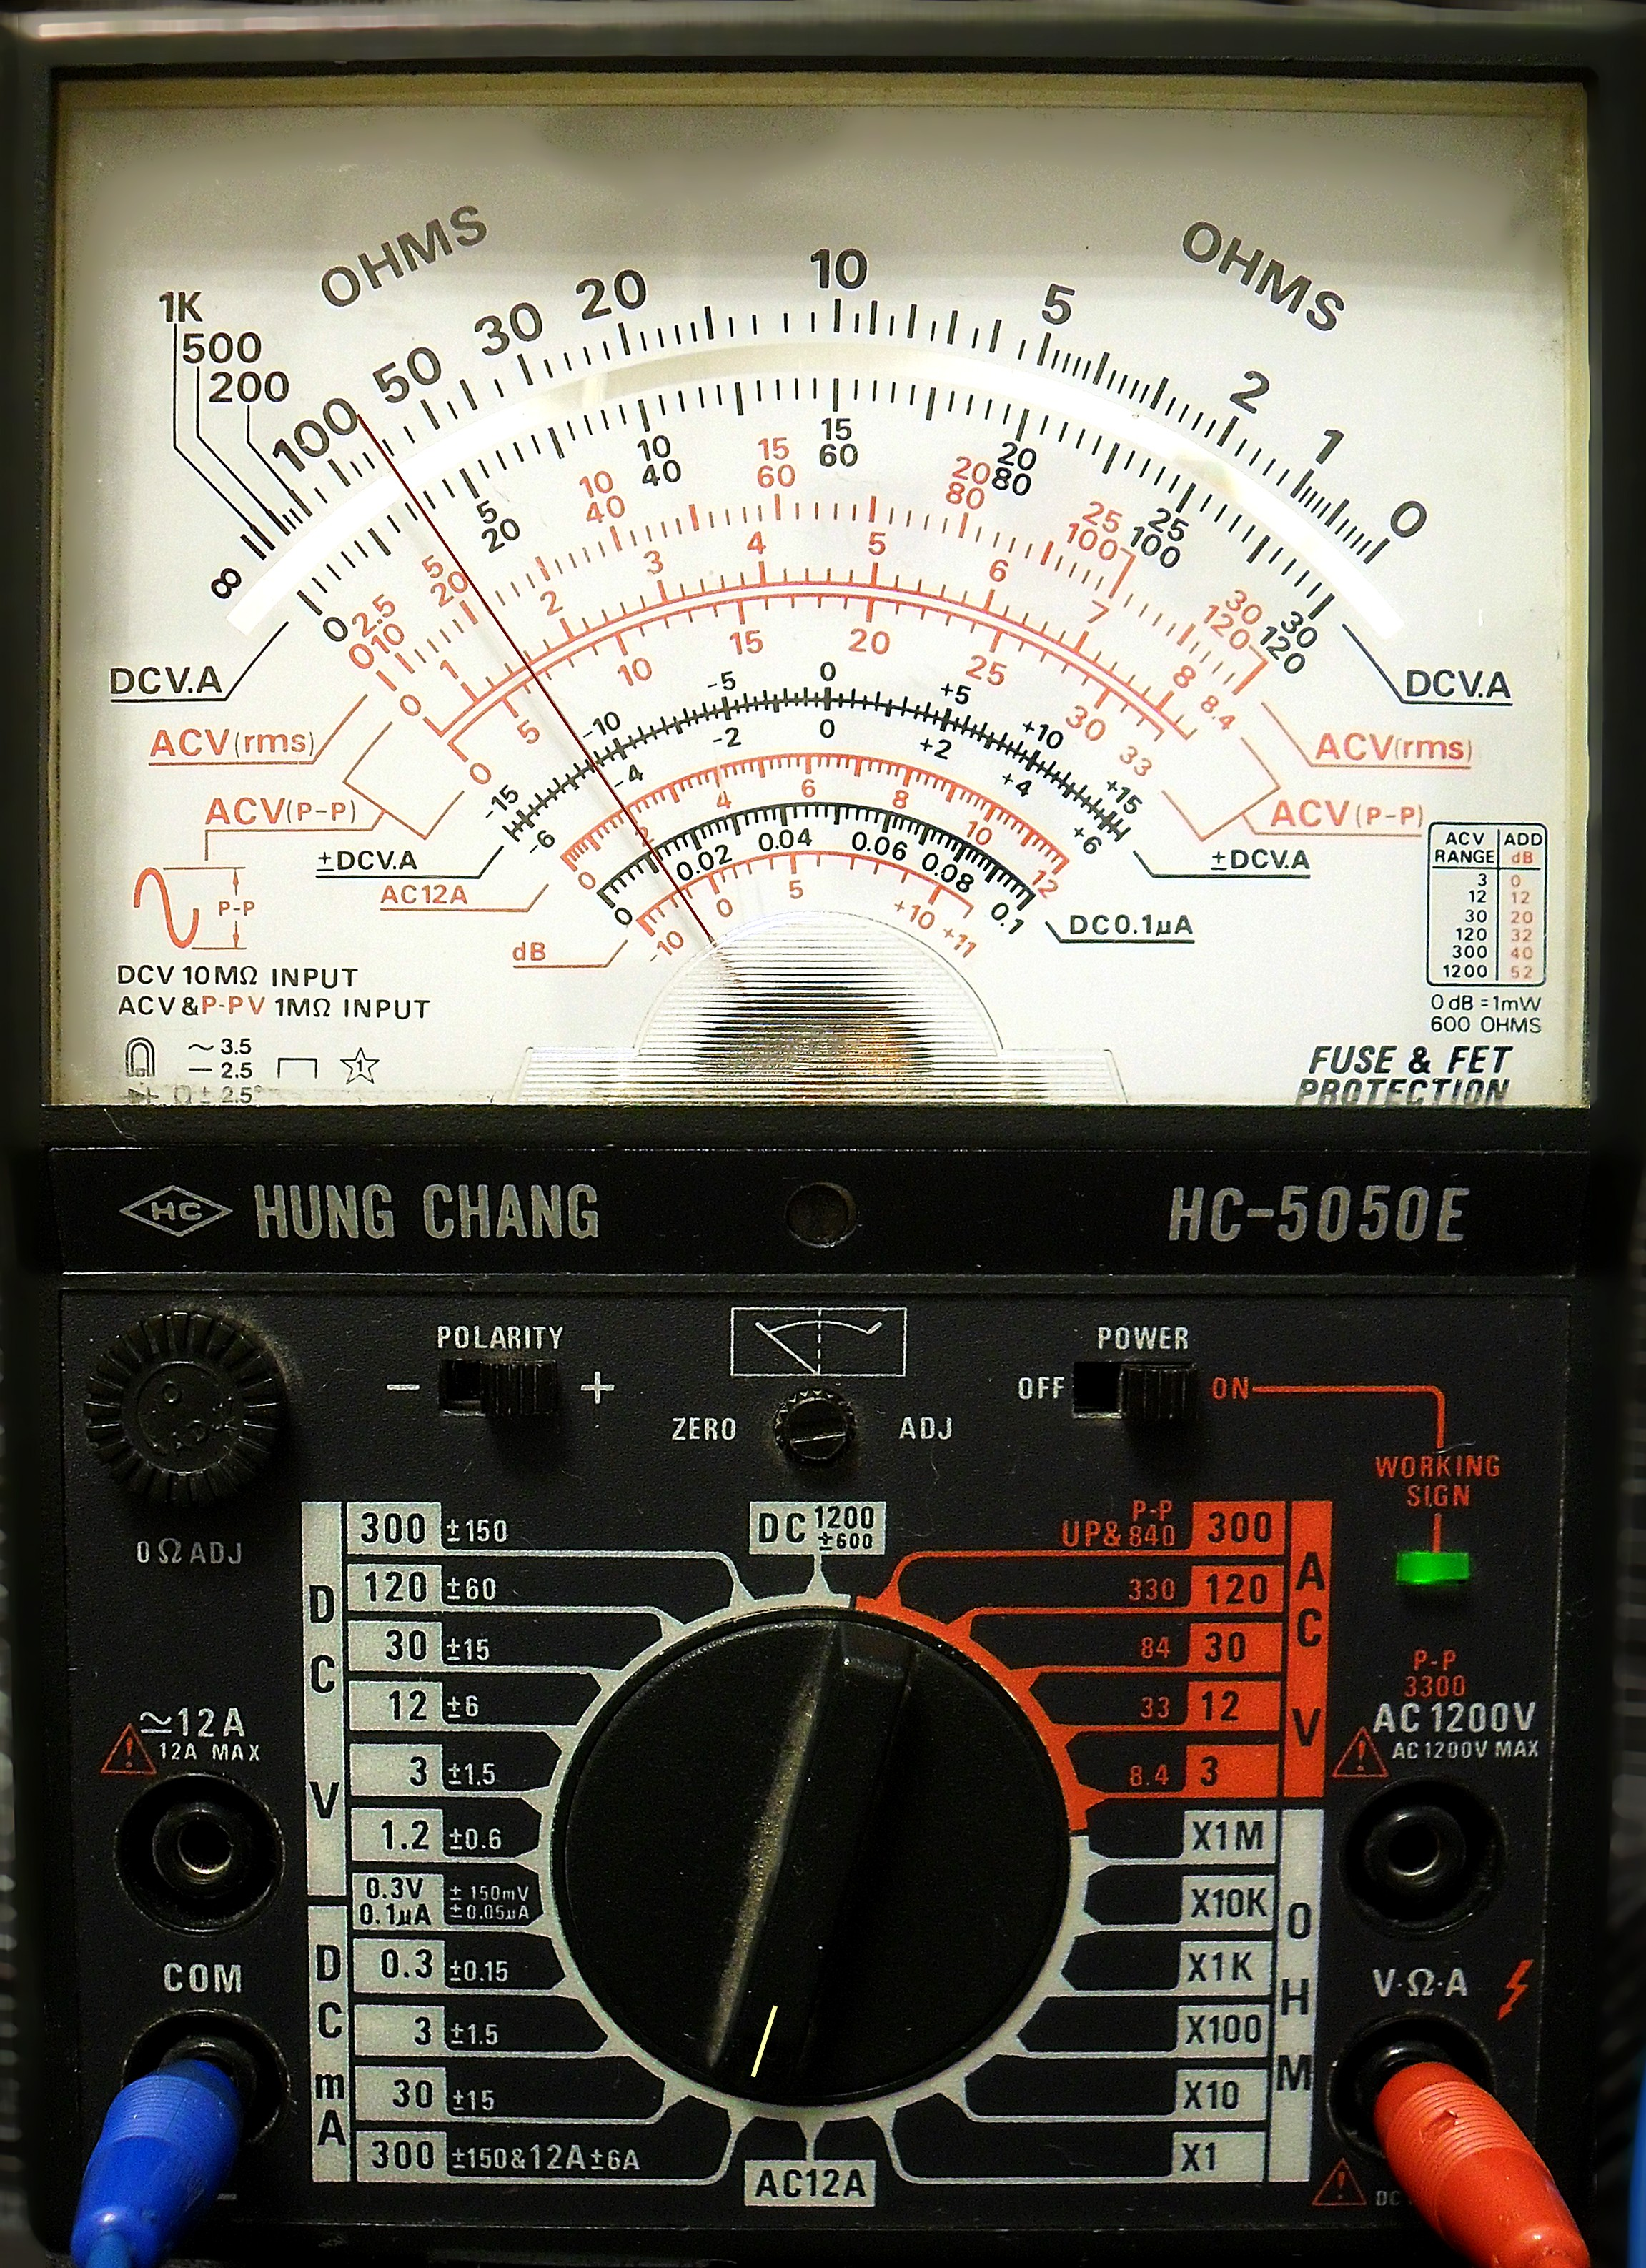
\includegraphics[width=0.85\textwidth]{foto/197}
    \caption{\scriptsize Zeigerinstrument mit mehreren Skalen}
    \label{e_zeigerinstrument}
\end{figure}

   \end{column}
\end{columns}

\end{frame}

\begin{frame}
\frametitle{Parallaxenfehler}
\begin{columns}
    \begin{column}{0.48\textwidth}
    \begin{itemize}
  \item Parallaxenfehler vermeiden, indem gerade drauf geschaut wird
  \item Viele Zeigerinstrumente haben einen Spiegel hinter dem Zeiger
  \item Wenn der Zeiger sich im Spiegelbild überdeckt, wird gerade drauf geschaut
  \end{itemize}

    \end{column}
   \begin{column}{0.48\textwidth}
       
\begin{figure}
    \includegraphics[width=0.85\textwidth]{foto/196}
    \caption{\scriptsize Zeigerinstrument mit Spiegel und Parallaxenfehler beim Ablesen}
    \label{e_parallaxenfehler}
\end{figure}

   \end{column}
\end{columns}

\end{frame}

\begin{frame}
\only<1>{
\begin{PQuestion}{EI103}{Welche Spannung wird bei dem folgenden Messinstrument angezeigt, wenn dessen Messbereich auf \qty{10}{\V} eingestellt ist? }{\qty{8,8}{\V}}
{\qty{29}{\V}}
{\qty{2,9}{\V}}
{\qty{88}{\V}}
{\DARCimage{1.0\linewidth}{41include}}\end{PQuestion}

}
\only<2>{
\begin{PQuestion}{EI103}{Welche Spannung wird bei dem folgenden Messinstrument angezeigt, wenn dessen Messbereich auf \qty{10}{\V} eingestellt ist? }{\qty{8,8}{\V}}
{\qty{29}{\V}}
{\textbf{\textcolor{DARCgreen}{\qty{2,9}{\V}}}}
{\qty{88}{\V}}
{\DARCimage{1.0\linewidth}{41include}}\end{PQuestion}

}
\end{frame}

\begin{frame}
\only<1>{
\begin{PQuestion}{EI104}{Welche Spannung wird bei dem folgenden Messinstrument angezeigt, wenn dessen Messbereich auf \qty{300}{\V} eingestellt ist?}{\qty{290}{\V}}
{\qty{29}{\V}}
{\qty{8,8}{\V}}
{\qty{88}{\V}}
{\DARCimage{1.0\linewidth}{41include}}\end{PQuestion}

}
\only<2>{
\begin{PQuestion}{EI104}{Welche Spannung wird bei dem folgenden Messinstrument angezeigt, wenn dessen Messbereich auf \qty{300}{\V} eingestellt ist?}{\qty{290}{\V}}
{\qty{29}{\V}}
{\qty{8,8}{\V}}
{\textbf{\textcolor{DARCgreen}{\qty{88}{\V}}}}
{\DARCimage{1.0\linewidth}{41include}}\end{PQuestion}

}
\end{frame}%ENDCONTENT


\section{Spitzen- und Effektivwert}
\label{section:spitze_effektiv_wert}
\begin{frame}%STARTCONTENT

\frametitle{Spitzenwert}
\begin{columns}
    \begin{column}{0.48\textwidth}
    \begin{itemize}
  \item Der Spitzenwert einer Sinusschwingung entspricht der Amplitude
  \item Von Nulllinie bis höchstem Wert
  \item Spitzen-Spitzen-Wert von niedrigstem bis höchstem Wert
  \end{itemize}

    \end{column}
   \begin{column}{0.48\textwidth}
       
\begin{figure}
    \DARCimage{0.85\linewidth}{834include}
    \caption{\scriptsize Peridoendauer, Spitzenspannung, Effektivspannung und Spitzen-Spitzen-Spannung}
    \label{e_spitze_effektiv_wert_bezeichnungen_sinus}
\end{figure}


   \end{column}
\end{columns}

\end{frame}

\begin{frame}Spitzen-Spitzen-Wert bei sinusförmigen Spannungen

$U_{SS} = 2\cdot \^{U}$

\end{frame}

\begin{frame}
\only<1>{
\begin{PQuestion}{EB407}{Wie groß ist der Spitzen-Spitzen-Wert ($U_{\symup{ss}}$) der in der Abbildung dargestellten Spannung?}{\qty{10}{\V}}
{\qty{20}{\V}}
{\qty{40}{\V}}
{\qty{4}{\V}}
{\DARCimage{1.0\linewidth}{52include}}\end{PQuestion}

}
\only<2>{
\begin{PQuestion}{EB407}{Wie groß ist der Spitzen-Spitzen-Wert ($U_{\symup{ss}}$) der in der Abbildung dargestellten Spannung?}{\qty{10}{\V}}
{\qty{20}{\V}}
{\textbf{\textcolor{DARCgreen}{\qty{40}{\V}}}}
{\qty{4}{\V}}
{\DARCimage{1.0\linewidth}{52include}}\end{PQuestion}

}
\end{frame}

\begin{frame}
\only<1>{
\begin{PQuestion}{EB406}{Wie groß ist der Spitzen-Spitzen-Wert der in diesem Schirmbild dargestellten Spannung?}{\qty{12}{\V}}
{\qty{6}{\V}}
{\qty{8,5}{\V}}
{\qty{2}{\V}}
{\DARCimage{1.0\linewidth}{53include}}\end{PQuestion}

}
\only<2>{
\begin{PQuestion}{EB406}{Wie groß ist der Spitzen-Spitzen-Wert der in diesem Schirmbild dargestellten Spannung?}{\textbf{\textcolor{DARCgreen}{\qty{12}{\V}}}}
{\qty{6}{\V}}
{\qty{8,5}{\V}}
{\qty{2}{\V}}
{\DARCimage{1.0\linewidth}{53include}}\end{PQuestion}

}
\end{frame}

\begin{frame}
\frametitle{Effektivwert}
Bei einer Wechselspannung der Wert, der in einem Widerstand zu einer vergleichsweisen Gleichspannung in Leistung umgesetzt wird


\begin{figure}
    \DARCimage{0.85\linewidth}{725include}
    \caption{\scriptsize Effektivwert und Spitzenwert der Spannung im Haushalt}
    \label{e_effektivwert_230v}
\end{figure}

\end{frame}

\begin{frame}Bei Spannungen (ohne Herleitung)

$\^{U} = U_{eff}\cdot \sqrt{2}$

\end{frame}

\begin{frame}
\only<1>{
\begin{PQuestion}{EB405}{Welche der im folgenden Diagramm eingezeichneten Gleichspannungen setzen an einem Wirkwiderstand etwa die gleiche Leistung um wie die dargestellte sinusförmige Wechselspannung?}{\qty{0}{\V}}
{\qty{1}{\V} und \qty{-1}{\V}}
{\qty{0,5}{\V} und \qty{-0,5}{\V}}
{\qty{0,7}{\V} und \qty{-0,7}{\V}}
{\DARCimage{1.0\linewidth}{206include}}\end{PQuestion}

}
\only<2>{
\begin{PQuestion}{EB405}{Welche der im folgenden Diagramm eingezeichneten Gleichspannungen setzen an einem Wirkwiderstand etwa die gleiche Leistung um wie die dargestellte sinusförmige Wechselspannung?}{\qty{0}{\V}}
{\qty{1}{\V} und \qty{-1}{\V}}
{\qty{0,5}{\V} und \qty{-0,5}{\V}}
{\textbf{\textcolor{DARCgreen}{\qty{0,7}{\V} und \qty{-0,7}{\V}}}}
{\DARCimage{1.0\linewidth}{206include}}\end{PQuestion}

}

\end{frame}

\begin{frame}
\frametitle{Lösungsweg}
$\^{U} = U_{eff}\cdot \sqrt{2}$

$U_{eff} = \dfrac{\^{U}}{\sqrt{2}}$

$U_{eff} = \dfrac{1V}{1,41} \approx 0,7V$

\end{frame}

\begin{frame}
\only<1>{
\begin{QQuestion}{EB404}{Eine sinusförmige Wechselspannung hat einen Spitzenwert von \qty{12}{\V}. Wie groß ist in etwa der Effektivwert der Wechselspannung?}{\qty{24}{\V}}
{\qty{6,0}{\V}}
{\qty{17}{\V}}
{\qty{8,5}{\V}}
\end{QQuestion}

}
\only<2>{
\begin{QQuestion}{EB404}{Eine sinusförmige Wechselspannung hat einen Spitzenwert von \qty{12}{\V}. Wie groß ist in etwa der Effektivwert der Wechselspannung?}{\qty{24}{\V}}
{\qty{6,0}{\V}}
{\qty{17}{\V}}
{\textbf{\textcolor{DARCgreen}{\qty{8,5}{\V}}}}
\end{QQuestion}

}

\end{frame}

\begin{frame}
\frametitle{Lösungsweg}
$\^{U} = U_{eff}\cdot \sqrt{2}$

$U_{eff} = \dfrac{\^{U}}{\sqrt{2}}$

$U_{eff} = \dfrac{12V}{1,41} \approx 8,5V$

\end{frame}

\begin{frame}
\only<1>{
\begin{QQuestion}{EB403}{Ein sinusförmiges Signal hat einen Effektivwert von \qty{12}{\V}. Wie groß ist in etwa der Spitzen-Spitzen-Wert?}{\qty{17}{\V}}
{\qty{24}{\V}}
{\qty{34}{\V}}
{\qty{8,5}{\V}}
\end{QQuestion}

}
\only<2>{
\begin{QQuestion}{EB403}{Ein sinusförmiges Signal hat einen Effektivwert von \qty{12}{\V}. Wie groß ist in etwa der Spitzen-Spitzen-Wert?}{\qty{17}{\V}}
{\qty{24}{\V}}
{\textbf{\textcolor{DARCgreen}{\qty{34}{\V}}}}
{\qty{8,5}{\V}}
\end{QQuestion}

}
\end{frame}

\begin{frame}
\frametitle{Lösungsweg}
$\^{U} = U_{eff}\cdot \sqrt{2}$

$\^{U} = 12V\cdot 1,41 \approx 17V$

$U_{SS} = 2\cdot \^{U}$

$U_{SS} = 2\cdot 17V = 34V$

\end{frame}

\begin{frame}
\only<1>{
\begin{QQuestion}{EB401}{Der Spitzenwert an einer häuslichen, einphasigen \qty{230}{\V}-Stromversorgung beträgt~...}{\qty{163}{\V}.}
{\qty{325}{\V}.}
{\qty{460}{\V}.}
{\qty{650}{\V}.}
\end{QQuestion}

}
\only<2>{
\begin{QQuestion}{EB401}{Der Spitzenwert an einer häuslichen, einphasigen \qty{230}{\V}-Stromversorgung beträgt~...}{\qty{163}{\V}.}
{\textbf{\textcolor{DARCgreen}{\qty{325}{\V}.}}}
{\qty{460}{\V}.}
{\qty{650}{\V}.}
\end{QQuestion}

}

\end{frame}

\begin{frame}
\frametitle{Lösungsweg}
$\^{U} = U_{eff}\cdot \sqrt{2}$

$\^{U} = 230V\cdot 1,41 \approx 325V$

\end{frame}

\begin{frame}
\only<1>{
\begin{QQuestion}{EB402}{Der Spitze-Spitze-Wert der häuslichen \qty{230}{\V}-Spannungsversorgung beträgt~...}{\qty{651}{\V}.}
{\qty{163}{\V}.}
{\qty{325}{\V}.}
{\qty{460}{\V}.}
\end{QQuestion}

}
\only<2>{
\begin{QQuestion}{EB402}{Der Spitze-Spitze-Wert der häuslichen \qty{230}{\V}-Spannungsversorgung beträgt~...}{\textbf{\textcolor{DARCgreen}{\qty{651}{\V}.}}}
{\qty{163}{\V}.}
{\qty{325}{\V}.}
{\qty{460}{\V}.}
\end{QQuestion}

}

\end{frame}%ENDCONTENT


\section{Oszilloskop I}
\label{section:oszilloskop_1}
\begin{frame}%STARTCONTENT

\frametitle{Periode}
\begin{columns}
    \begin{column}{0.48\textwidth}
    \begin{itemize}
  \item Dauer einer vollständigen Schwingung
  \item Wird zur Ermittlung der Frequenz benötigt, z.B. Oszilloskop
  \end{itemize}

    \end{column}
   \begin{column}{0.48\textwidth}
       
\begin{figure}
    \DARCimage{0.85\linewidth}{790include}
    \caption{\scriptsize Periode und Amplitude in einer Sinusschwingung}
    \label{e_periode_amplitude}
\end{figure}


   \end{column}
\end{columns}

\end{frame}

\begin{frame}\begin{itemize}
  \item Periode steht im umgekehrten Verhältnis zur Frequenz
  \item Formelzeichen T, Einheit Sekunde (s)
  \end{itemize}
    \pause
    $T = \dfrac{1}{f} \Rightarrow f = \dfrac{1}{T}$



\end{frame}

\begin{frame}\end{frame}

\begin{frame}
\only<1>{
\begin{QQuestion}{EB408}{Die Periodendauer von \qty{50}{\us} entspricht einer Frequenz von~...}{\qty{2}{\MHz}.}
{\qty{20}{\kHz}.}
{\qty{200}{\kHz}.}
{\qty{20}{\MHz}.}
\end{QQuestion}

}
\only<2>{
\begin{QQuestion}{EB408}{Die Periodendauer von \qty{50}{\us} entspricht einer Frequenz von~...}{\qty{2}{\MHz}.}
{\textbf{\textcolor{DARCgreen}{\qty{20}{\kHz}.}}}
{\qty{200}{\kHz}.}
{\qty{20}{\MHz}.}
\end{QQuestion}

}
\end{frame}

\begin{frame}
\frametitle{Periodendauer ablesen}
\begin{columns}
    \begin{column}{0.48\textwidth}
    \begin{itemize}
  \item Kästchen einer ganzen Periode im Nulldurchgang zählen
  \item Mit der Zeiteinheit multiplizieren
  \item Bei 8 Kästchen und 2 ms pro Kästchen $\rightarrow$ 8 $\cdot$ 2 ms = 16 ms
  \end{itemize}

    \end{column}
   \begin{column}{0.48\textwidth}
       
\begin{figure}
    \DARCimage{0.85\linewidth}{36include}
    \caption{\scriptsize Eine Sinuswelle auf dem Bildschirm eine Oszilloskops}
    \label{e_sinuswelle_oszilloskop}
\end{figure}


   \end{column}
\end{columns}

\end{frame}

\begin{frame}
\only<1>{
\begin{PQuestion}{EI301}{Die Zeitbasis eines Oszilloskop ist so eingestellt, dass ein Skalenteil \qty{0,5}{\ms} entspricht. Welche Periodendauer hat die angelegte Spannung?}{\qty{4}{\ms}}
{\qty{2}{\ms}}
{\qty{1,5}{\ms}}
{\qty{3}{\ms}}
{\DARCimage{1.0\linewidth}{36include}}\end{PQuestion}

}
\only<2>{
\begin{PQuestion}{EI301}{Die Zeitbasis eines Oszilloskop ist so eingestellt, dass ein Skalenteil \qty{0,5}{\ms} entspricht. Welche Periodendauer hat die angelegte Spannung?}{\textbf{\textcolor{DARCgreen}{\qty{4}{\ms}}}}
{\qty{2}{\ms}}
{\qty{1,5}{\ms}}
{\qty{3}{\ms}}
{\DARCimage{1.0\linewidth}{36include}}\end{PQuestion}

}
\end{frame}

\begin{frame}
\frametitle{Frequenz ermitteln}
$f = \dfrac{1}{T}$

Erst Periodendauer ermitteln, dann Frequenz ausrechnen

\end{frame}

\begin{frame}
\only<1>{
\begin{PQuestion}{EB410}{Welche Frequenz hat die in diesem Oszillogramm dargestellte Spannung?}{\qty{50}{\Hz}}
{\qty{100}{\Hz}}
{\qty{500}{\Hz}}
{\qty{20}{\Hz}}
{\DARCimage{1.0\linewidth}{56include}}\end{PQuestion}

}
\only<2>{
\begin{PQuestion}{EB410}{Welche Frequenz hat die in diesem Oszillogramm dargestellte Spannung?}{\textbf{\textcolor{DARCgreen}{\qty{50}{\Hz}}}}
{\qty{100}{\Hz}}
{\qty{500}{\Hz}}
{\qty{20}{\Hz}}
{\DARCimage{1.0\linewidth}{56include}}\end{PQuestion}

}

\end{frame}

\begin{frame}
\frametitle{Lösungsweg}
Eine Periode ist 4 Kästchen lang

$T = 4\cdot 5ms = 20ms$

$f = \dfrac{1}{T} = \dfrac{1}{20\cdot10^{-3}s} = $

$0,05\frac{1}{10^{-3}s} = 0,05\cdot10^3Hz = 0,05kHz = 50Hz$

\end{frame}

\begin{frame}
\only<1>{
\begin{PQuestion}{EI302}{Die Zeitbasis eines Oszilloskops ist so eingestellt, dass ein Skalenteil \qty{0,5}{\ms} entspricht. Welche Frequenz hat die angelegte Spannung? }{\qty{500}{\Hz}}
{\qty{250}{\Hz}}
{\qty{667}{\Hz}}
{\qty{333}{\Hz}}
{\DARCimage{1.0\linewidth}{36include}}\end{PQuestion}

}
\only<2>{
\begin{PQuestion}{EI302}{Die Zeitbasis eines Oszilloskops ist so eingestellt, dass ein Skalenteil \qty{0,5}{\ms} entspricht. Welche Frequenz hat die angelegte Spannung? }{\qty{500}{\Hz}}
{\textbf{\textcolor{DARCgreen}{\qty{250}{\Hz}}}}
{\qty{667}{\Hz}}
{\qty{333}{\Hz}}
{\DARCimage{1.0\linewidth}{36include}}\end{PQuestion}

}
\end{frame}

\begin{frame}
\only<1>{
\begin{PQuestion}{EB409}{Welche Frequenz hat die in diesem Oszillogramm dargestellte Spannung in etwa?}{\qty{833}{\kHz}}
{\qty{83,3}{\kHz}}
{\qty{8,33}{\MHz}}
{\qty{83,3}{\MHz}}
{\DARCimage{1.0\linewidth}{53include}}\end{PQuestion}

}
\only<2>{
\begin{PQuestion}{EB409}{Welche Frequenz hat die in diesem Oszillogramm dargestellte Spannung in etwa?}{\qty{833}{\kHz}}
{\textbf{\textcolor{DARCgreen}{\qty{83,3}{\kHz}}}}
{\qty{8,33}{\MHz}}
{\qty{83,3}{\MHz}}
{\DARCimage{1.0\linewidth}{53include}}\end{PQuestion}

}

\end{frame}

\begin{frame}
\frametitle{Lösungsweg}
Eine Periode ist 4 Kästchen lang

$T = 4\cdot 3\mu s = 12\mu s$

$f = \dfrac{1}{T} = \dfrac{1}{12\cdot10^{-6}s} = $

$0,0833\frac{1}{10^{-6}s} = 0,0833\cdot10^6Hz = 0,0833MHz = 83,3kHz$

\end{frame}

\begin{frame}
\only<1>{
\begin{PQuestion}{EB411}{Welche Frequenz hat das in diesem Schirmbild dargestellte Signal?}{\qty{8,33}{\MHz}}
{\qty{83,3}{\MHz}}
{\qty{8,33}{\kHz}}
{\qty{833}{\kHz}}
{\DARCimage{1.0\linewidth}{55include}}\end{PQuestion}

}
\only<2>{
\begin{PQuestion}{EB411}{Welche Frequenz hat das in diesem Schirmbild dargestellte Signal?}{\textbf{\textcolor{DARCgreen}{\qty{8,33}{\MHz}}}}
{\qty{83,3}{\MHz}}
{\qty{8,33}{\kHz}}
{\qty{833}{\kHz}}
{\DARCimage{1.0\linewidth}{55include}}\end{PQuestion}

}
\end{frame}

\begin{frame}
\frametitle{Impuls}
\begin{columns}
    \begin{column}{0.48\textwidth}
    \begin{itemize}
  \item Ein Signal springt von einem Wert auf einen höheren und zu einem späteren Zeitpunkt zurück
  \item Dauer des Impulses wird von Mitte der ansteigenden Flanke bis zur Mitte der abfallenden Flanke gemessen
  \end{itemize}

    \end{column}
   \begin{column}{0.48\textwidth}
       
\begin{figure}
    \DARCimage{0.85\linewidth}{57include}
    \caption{\scriptsize Impuls in einem Oszilloskop}
    \label{e_impuls}
\end{figure}

 
   \end{column}
\end{columns}

\end{frame}

\begin{frame}
\only<1>{
\begin{PQuestion}{EI303}{Die Impulsdauer beträgt hier~...}{\qty{230}{\micro\s}.}
{\qty{260}{\micro\s}.}
{\qty{200}{\micro\s}.}
{\qty{150}{\micro\s}.}
{\DARCimage{1.0\linewidth}{57include}}\end{PQuestion}

}
\only<2>{
\begin{PQuestion}{EI303}{Die Impulsdauer beträgt hier~...}{\qty{230}{\micro\s}.}
{\qty{260}{\micro\s}.}
{\textbf{\textcolor{DARCgreen}{\qty{200}{\micro\s}.}}}
{\qty{150}{\micro\s}.}
{\DARCimage{1.0\linewidth}{57include}}\end{PQuestion}

}
\end{frame}

\begin{frame}
\frametitle{NF-Verzerrungen}
\begin{itemize}
  \item Verzerrungen sind Abweichungen von der Sinusform
  \item Diese können mit einem Oszilloskop sichtbar gemacht werden
  \end{itemize}
\end{frame}

\begin{frame}
\only<1>{
\begin{QQuestion}{EI304}{Welches dieser Geräte wird für die Anzeige von NF-Verzerrungen verwendet?}{Ein Oszilloskop}
{Ein Transistorvoltmeter}
{Ein Vielfachmessgerät}
{Ein Frequenzzähler}
\end{QQuestion}

}
\only<2>{
\begin{QQuestion}{EI304}{Welches dieser Geräte wird für die Anzeige von NF-Verzerrungen verwendet?}{\textbf{\textcolor{DARCgreen}{Ein Oszilloskop}}}
{Ein Transistorvoltmeter}
{Ein Vielfachmessgerät}
{Ein Frequenzzähler}
\end{QQuestion}

}
\end{frame}%ENDCONTENT


\section{SMD-Widerstände}
\label{section:widerstand_smd}
\begin{frame}%STARTCONTENT

\begin{columns}
    \begin{column}{0.48\textwidth}
    \begin{itemize}
  \item SMD: Surface Mounted Device
  \item Widerstand in sehr kleiner Bauform
  \item Letzte Stelle des aufgedruckten Widerstandswerts gibt die Zehnerpotenz an
  \end{itemize}

    \end{column}
   \begin{column}{0.48\textwidth}
       
\begin{figure}
    \DARCimage{0.85\linewidth}{529include}
    \caption{\scriptsize SMD-Widerstand}
    \label{e_smd_widerstand}
\end{figure}


   \end{column}
\end{columns}

\end{frame}

\begin{frame}
\only<1>{
\begin{QQuestion}{EC114}{Wie wird in der Regel bei SMD-Widerständen der Widerstandswert angegeben?}{Auf dem Widerstand ist der Wert in Form von Zahlen abgedruckt, wobei die letzte Ziffer die Zehnerpotenz angibt.}
{Auf dem Widerstand ist der Wert in Form von Farbringen aufgedruckt, wobei der letzte Farbring die Toleranz angibt.}
{Auf dem Widerstand ist der Wert in Form von Farbringen aufgedruckt, wobei der letzte Farbring die Zehnerpotenz angibt.}
{Auf dem Widerstand ist der Wert in Form von Zahlen abgedruckt, wobei die angegebene Zahl dem Wert des Widerstands entspricht.}
\end{QQuestion}

}
\only<2>{
\begin{QQuestion}{EC114}{Wie wird in der Regel bei SMD-Widerständen der Widerstandswert angegeben?}{\textbf{\textcolor{DARCgreen}{Auf dem Widerstand ist der Wert in Form von Zahlen abgedruckt, wobei die letzte Ziffer die Zehnerpotenz angibt.}}}
{Auf dem Widerstand ist der Wert in Form von Farbringen aufgedruckt, wobei der letzte Farbring die Toleranz angibt.}
{Auf dem Widerstand ist der Wert in Form von Farbringen aufgedruckt, wobei der letzte Farbring die Zehnerpotenz angibt.}
{Auf dem Widerstand ist der Wert in Form von Zahlen abgedruckt, wobei die angegebene Zahl dem Wert des Widerstands entspricht.}
\end{QQuestion}

}
\end{frame}

\begin{frame}
\only<1>{
\begin{PQuestion}{EC115}{Welchen Wert hat der dargestellte SMD-Widerstand?}{\qty{103}{\ohm}}
{\qty{10}{\kohm}}
{\qty{1}{\kohm}}
{\qty{10,3}{\ohm}}
{\DARCimage{0.5\linewidth}{529include}}\end{PQuestion}

}
\only<2>{
\begin{PQuestion}{EC115}{Welchen Wert hat der dargestellte SMD-Widerstand?}{\qty{103}{\ohm}}
{\textbf{\textcolor{DARCgreen}{\qty{10}{\kohm}}}}
{\qty{1}{\kohm}}
{\qty{10,3}{\ohm}}
{\DARCimage{0.5\linewidth}{529include}}\end{PQuestion}

}
\end{frame}

\begin{frame}
\only<1>{
\begin{QQuestion}{EC116}{Welchen Wert hat ein SMD-Widerstand mit der Kennzeichnung 221?}{\qty{220}{\ohm}}
{\qty{221}{\ohm}}
{\qty{22,0}{\ohm}}
{\qty{22,1}{\ohm}}
\end{QQuestion}

}
\only<2>{
\begin{QQuestion}{EC116}{Welchen Wert hat ein SMD-Widerstand mit der Kennzeichnung 221?}{\textbf{\textcolor{DARCgreen}{\qty{220}{\ohm}}}}
{\qty{221}{\ohm}}
{\qty{22,0}{\ohm}}
{\qty{22,1}{\ohm}}
\end{QQuestion}

}
\end{frame}

\begin{frame}
\only<1>{
\begin{QQuestion}{EC117}{Welchen Wert hat ein SMD-Widerstand mit der Kennzeichnung 223?}{\qty{223}{\ohm}}
{\qty{22}{\kohm}}
{\qty{22,3}{\kohm}}
{\qty{220}{\ohm}}
\end{QQuestion}

}
\only<2>{
\begin{QQuestion}{EC117}{Welchen Wert hat ein SMD-Widerstand mit der Kennzeichnung 223?}{\qty{223}{\ohm}}
{\textbf{\textcolor{DARCgreen}{\qty{22}{\kohm}}}}
{\qty{22,3}{\kohm}}
{\qty{220}{\ohm}}
\end{QQuestion}

}
\end{frame}%ENDCONTENT


\section{Widerstandsmaterialien}
\label{section:widerstand_materialien}
\begin{frame}%STARTCONTENT

\frametitle{Drahtwiderstände}
\begin{itemize}
  \item Draht aus einem Leiter mit gutem konstanten Widerstand trotz ändernder Temperatur
  \item Dadurch ist eine hohe Last möglich
  \item Oftmals gewickelt für mehr Länge
  \item Dadurch nur für niedrige Frequenzen geeignet
  \end{itemize}
\end{frame}

\begin{frame}
\only<1>{
\begin{QQuestion}{EC101}{Welche Widerstände sind besonders als Hochlastwiderstände bei niedrigen Frequenzen geeignet?}{Drahtwiderstände}
{Metallschichtwiderstände}
{Metalloxidschichtwiderstände}
{LDR-Widerstände}
\end{QQuestion}

}
\only<2>{
\begin{QQuestion}{EC101}{Welche Widerstände sind besonders als Hochlastwiderstände bei niedrigen Frequenzen geeignet?}{\textbf{\textcolor{DARCgreen}{Drahtwiderstände}}}
{Metallschichtwiderstände}
{Metalloxidschichtwiderstände}
{LDR-Widerstände}
\end{QQuestion}

}
\end{frame}

\begin{frame}
\frametitle{Metallschichtwiderstand}
\begin{itemize}
  \item Widerstandsmaterial als dünne Schicht auf einem Träger
  \item Hohe Widerstandswerte möglich
  \item Sehr präzise
  \item Geringe Temperaturabhängigkeit
  \end{itemize}
\end{frame}

\begin{frame}
\only<1>{
\begin{QQuestion}{EC102}{Welche Widerstände haben geringe Fertigungstoleranzen und Temperaturabhängigkeit und sind besonders als Präzisionswiderstände geeignet?}{Metallschichtwiderstände}
{Metalloxidschichtwiderstände}
{Drahtwiderstände}
{LDR-Widerstände}
\end{QQuestion}

}
\only<2>{
\begin{QQuestion}{EC102}{Welche Widerstände haben geringe Fertigungstoleranzen und Temperaturabhängigkeit und sind besonders als Präzisionswiderstände geeignet?}{\textbf{\textcolor{DARCgreen}{Metallschichtwiderstände}}}
{Metalloxidschichtwiderstände}
{Drahtwiderstände}
{LDR-Widerstände}
\end{QQuestion}

}
\end{frame}

\begin{frame}
\frametitle{Metalloxid&shy;schicht&shy;widerstand}
\begin{itemize}
  \item Ähnlich wie Metallschichtwiderstand
  \item Induktionsarm
  \item Für hohe Frequenzen geeignet
  \end{itemize}
\end{frame}

\begin{frame}
\only<1>{
\begin{QQuestion}{EC103}{Welche Widerstände sind induktionsarm und eignen sich besonders für den Einsatz bei Frequenzen oberhalb von \qty{30}{\MHz}.}{LDR-Widerstände}
{Metallschichtwiderstände}
{Drahtwiderstände}
{Metalloxidschichtwiderstände}
\end{QQuestion}

}
\only<2>{
\begin{QQuestion}{EC103}{Welche Widerstände sind induktionsarm und eignen sich besonders für den Einsatz bei Frequenzen oberhalb von \qty{30}{\MHz}.}{LDR-Widerstände}
{Metallschichtwiderstände}
{Drahtwiderstände}
{\textbf{\textcolor{DARCgreen}{Metalloxidschichtwiderstände}}}
\end{QQuestion}

}
\end{frame}

\begin{frame}
\only<1>{
\begin{QQuestion}{EC104}{Welche Eigenschaft sollten Bauteile aufweisen, welche für den Bau von künstlichen Antennen (Dummy Load) zum Einsatz im VHF- und UHF-Bereich verwendet werden.}{geringen elektrischen und elektronischen Leitwert}
{geringe Eigeninduktivität und Eigenkapazität}
{hohe Eigeninduktivität und Eigenkapazität}
{hohen elektrischen und elektronischen Leitwert}
\end{QQuestion}

}
\only<2>{
\begin{QQuestion}{EC104}{Welche Eigenschaft sollten Bauteile aufweisen, welche für den Bau von künstlichen Antennen (Dummy Load) zum Einsatz im VHF- und UHF-Bereich verwendet werden.}{geringen elektrischen und elektronischen Leitwert}
{\textbf{\textcolor{DARCgreen}{geringe Eigeninduktivität und Eigenkapazität}}}
{hohe Eigeninduktivität und Eigenkapazität}
{hohen elektrischen und elektronischen Leitwert}
\end{QQuestion}

}

\end{frame}%ENDCONTENT


\section{Widerstandstoleranzen}
\label{section:widerstand_toleranz}
\begin{frame}%STARTCONTENT
\begin{itemize}
  \item Einfache Prozentrechnung
  \item Korrektur nach unten und oben vom angegebenen Widerstandswert
  \end{itemize}
\end{frame}

\begin{frame}
\only<1>{
\begin{QQuestion}{EC112}{Ein Widerstand hat eine Toleranz von \qty{10}{\percent}. Bei einem nominalen Widerstandswert von \qty{5,6}{\kohm} liegt der tatsächliche Wert zwischen~...}{\qtyrange{4760}{6440}{\ohm}.}
{\qtyrange{5040}{6160}{\ohm}.}
{\qtyrange{4,7}{6,8}{\kohm}.}
{\qtyrange{5,2}{6,3}{\kohm}.}
\end{QQuestion}

}
\only<2>{
\begin{QQuestion}{EC112}{Ein Widerstand hat eine Toleranz von \qty{10}{\percent}. Bei einem nominalen Widerstandswert von \qty{5,6}{\kohm} liegt der tatsächliche Wert zwischen~...}{\qtyrange{4760}{6440}{\ohm}.}
{\textbf{\textcolor{DARCgreen}{\qtyrange{5040}{6160}{\ohm}.}}}
{\qtyrange{4,7}{6,8}{\kohm}.}
{\qtyrange{5,2}{6,3}{\kohm}.}
\end{QQuestion}

}
\end{frame}

\begin{frame}
\only<1>{
\begin{QQuestion}{EC113}{Die Farbringe grün, blau und rot sowie ein silberner auf einem Widerstand mit 4 Farbringen bedeuten einen Widerstandswert zwischen~...}{\qtyrange{5240}{6360}{\ohm}.}
{\qtyrange{4760}{6440}{\ohm}.}
{\qtyrange{4760}{6840}{\ohm}.}
{\qtyrange{5040}{6160}{\ohm}.}
\end{QQuestion}

}
\only<2>{
\begin{QQuestion}{EC113}{Die Farbringe grün, blau und rot sowie ein silberner auf einem Widerstand mit 4 Farbringen bedeuten einen Widerstandswert zwischen~...}{\qtyrange{5240}{6360}{\ohm}.}
{\qtyrange{4760}{6440}{\ohm}.}
{\qtyrange{4760}{6840}{\ohm}.}
{\textbf{\textcolor{DARCgreen}{\qtyrange{5040}{6160}{\ohm}.}}}
\end{QQuestion}

}
\end{frame}%ENDCONTENT


\section{Heißleiter und Kaltleiter}
\label{section:widerstand_ntc_ptc}
\begin{frame}%STARTCONTENT

\frametitle{Heißleiter}
\begin{columns}
    \begin{column}{0.48\textwidth}
    \begin{itemize}
  \item Heißleiter ist ein temperaturabhängiger Widerstand
  \item Englisch: Negative Temperature Coefficient Thermistor (\emph{NTC})
  \item Leitet bei \emph{hohen Temperaturen} elektrischen Strom besser
  \end{itemize}

    \end{column}
   \begin{column}{0.48\textwidth}
       
\begin{figure}
    \DARCimage{0.85\linewidth}{125include}
    \caption{\scriptsize Schaltzeichen eines NTC-Widerstands}
    \label{e_ntc}
\end{figure}


   \end{column}
\end{columns}

\end{frame}

\begin{frame}
\only<1>{
\begin{PQuestion}{EC109}{Welches Bauteil hat folgendes Schaltzeichen?}{VDR}
{PTC}
{LDR}
{NTC}
{\DARCimage{0.5\linewidth}{125include}}\end{PQuestion}

}
\only<2>{
\begin{PQuestion}{EC109}{Welches Bauteil hat folgendes Schaltzeichen?}{VDR}
{PTC}
{LDR}
{\textbf{\textcolor{DARCgreen}{NTC}}}
{\DARCimage{0.5\linewidth}{125include}}\end{PQuestion}

}
\end{frame}

\begin{frame}
\only<1>{
\begin{question2x2}{EC110}{Welches der folgenden Bauteile ist ein NTC-Widerstand?}{\DARCimage{1.0\linewidth}{128include}}
{\DARCimage{1.0\linewidth}{126include}}
{\DARCimage{1.0\linewidth}{127include}}
{\DARCimage{1.0\linewidth}{125include}}
\end{question2x2}

}
\only<2>{
\begin{question2x2}{EC110}{Welches der folgenden Bauteile ist ein NTC-Widerstand?}{\DARCimage{1.0\linewidth}{128include}}
{\DARCimage{1.0\linewidth}{126include}}
{\DARCimage{1.0\linewidth}{127include}}
{\textbf{\textcolor{DARCgreen}{\DARCimage{1.0\linewidth}{125include}}}}
\end{question2x2}

}
\end{frame}

\begin{frame}
\frametitle{Kaltleiter}
\begin{columns}
    \begin{column}{0.48\textwidth}
    \begin{itemize}
  \item Kaltleiter ist ein temperaturabhängiger Widerstand
  \item Englisch: Positive Temperature Coefficient Thermistor (\emph{PTC})
  \item Leitet bei \emph{tiefen Temperaturen} elektrischen Strom besser
  \end{itemize}

    \end{column}
   \begin{column}{0.48\textwidth}
       
\begin{figure}
    \DARCimage{0.85\linewidth}{126include}
    \caption{\scriptsize Schaltzeichen eines PTC-Widerstands}
    \label{e_ptc}
\end{figure}


   \end{column}
\end{columns}

\end{frame}

\begin{frame}
\only<1>{
\begin{question2x2}{EC111}{Welches der folgenden Schaltsymbole stellt einen PTC-Widerstand dar?}{\DARCimage{1.0\linewidth}{126include}}
{\DARCimage{1.0\linewidth}{125include}}
{\DARCimage{1.0\linewidth}{127include}}
{\DARCimage{1.0\linewidth}{128include}}
\end{question2x2}

}
\only<2>{
\begin{question2x2}{EC111}{Welches der folgenden Schaltsymbole stellt einen PTC-Widerstand dar?}{\textbf{\textcolor{DARCgreen}{\DARCimage{1.0\linewidth}{126include}}}}
{\DARCimage{1.0\linewidth}{125include}}
{\DARCimage{1.0\linewidth}{127include}}
{\DARCimage{1.0\linewidth}{128include}}
\end{question2x2}

}
\end{frame}%ENDCONTENT


\section{Leistung II}
\label{section:leistung_2}
\begin{frame}%STARTCONTENT

\frametitle{Leistungsberechnung}
Wir kennen bereits

$P = U\cdot I = \dfrac{U^2}{R} = I^2\cdot R$
\begin{columns}
    \begin{column}{0.48\textwidth}
    Nach U umgestellt:

$U = \dfrac{P}{I} = \sqrt{P \cdot R}$


    \end{column}
   \begin{column}{0.48\textwidth}
       Nach I umgestellt:

$I = \dfrac{P}{U} = \sqrt{\dfrac{P}{R}}$


   \end{column}
\end{columns}

\end{frame}

\begin{frame}
\only<1>{
\begin{QQuestion}{EB505}{In welcher Antwort sind alle dargestellten Zusammenhänge zwischen Strom, Spannung, Widerstand und Leistung richtig?}{$I = \dfrac{\sqrt{P}}{R};\quad U = \sqrt{P}\cdot R$}
{$I = \sqrt{P\cdot R};\quad U = \sqrt{\dfrac{P}{R}}$}
{$I = \sqrt{\dfrac{R}{P}};\quad U = \sqrt{P\cdot R}$}
{$I = \sqrt{\dfrac{P}{R}};\quad U = \sqrt{P\cdot R}$}
\end{QQuestion}

}
\only<2>{
\begin{QQuestion}{EB505}{In welcher Antwort sind alle dargestellten Zusammenhänge zwischen Strom, Spannung, Widerstand und Leistung richtig?}{$I = \dfrac{\sqrt{P}}{R};\quad U = \sqrt{P}\cdot R$}
{$I = \sqrt{P\cdot R};\quad U = \sqrt{\dfrac{P}{R}}$}
{$I = \sqrt{\dfrac{R}{P}};\quad U = \sqrt{P\cdot R}$}
{\textbf{\textcolor{DARCgreen}{$I = \sqrt{\dfrac{P}{R}};\quad U = \sqrt{P\cdot R}$}}}
\end{QQuestion}

}
\end{frame}

\begin{frame}
\only<1>{
\begin{QQuestion}{EB506}{In welcher Antwort sind alle dargestellten Zusammenhänge zwischen Widerstand, Leistung, Spannung und Strom richtig?}{$R = \dfrac{U^2}{P};\quad R = \dfrac{P}{I^2}$}
{$R = U^2\cdot I;\quad R = \dfrac{P}{I^2}$}
{$R = \dfrac{P}{U^2};\quad R = P\cdot I^2$}
{$R = \dfrac{U^2}{P};\quad R = P\cdot I^2$}
\end{QQuestion}

}
\only<2>{
\begin{QQuestion}{EB506}{In welcher Antwort sind alle dargestellten Zusammenhänge zwischen Widerstand, Leistung, Spannung und Strom richtig?}{\textbf{\textcolor{DARCgreen}{$R = \dfrac{U^2}{P};\quad R = \dfrac{P}{I^2}$}}}
{$R = U^2\cdot I;\quad R = \dfrac{P}{I^2}$}
{$R = \dfrac{P}{U^2};\quad R = P\cdot I^2$}
{$R = \dfrac{U^2}{P};\quad R = P\cdot I^2$}
\end{QQuestion}

}
\end{frame}

\begin{frame}
\only<1>{
\begin{QQuestion}{EB504}{An einem Widerstand $R$ wird die elektrische Leistung $P$ in Wärme umgesetzt. Sie kennen die Größen $P$ und $R$. Nach welcher der Formeln können Sie die Spannung ermitteln, die an dem Widerstand $R$ anliegt?}{$U = \dfrac{P}{R}$}
{$U = R\cdot P$}
{$U = \sqrt{\dfrac{P}{R}}$}
{$U = \sqrt{P\cdot R}$}
\end{QQuestion}

}
\only<2>{
\begin{QQuestion}{EB504}{An einem Widerstand $R$ wird die elektrische Leistung $P$ in Wärme umgesetzt. Sie kennen die Größen $P$ und $R$. Nach welcher der Formeln können Sie die Spannung ermitteln, die an dem Widerstand $R$ anliegt?}{$U = \dfrac{P}{R}$}
{$U = R\cdot P$}
{$U = \sqrt{\dfrac{P}{R}}$}
{\textbf{\textcolor{DARCgreen}{$U = \sqrt{P\cdot R}$}}}
\end{QQuestion}

}
\end{frame}

\begin{frame}
\only<1>{
\begin{QQuestion}{EB507}{Der Effektivwert der Spannung an einer künstlichen \qty{50}{\ohm}-Antenne wird mit \qty{100}{\V} gemessen. Die Leistung an der Last beträgt~...}{\qty{100}{\W}.}
{\qty{50}{\W}.}
{\qty{200}{\W}.}
{\qty{400}{\W}.}
\end{QQuestion}

}
\only<2>{
\begin{QQuestion}{EB507}{Der Effektivwert der Spannung an einer künstlichen \qty{50}{\ohm}-Antenne wird mit \qty{100}{\V} gemessen. Die Leistung an der Last beträgt~...}{\qty{100}{\W}.}
{\qty{50}{\W}.}
{\textbf{\textcolor{DARCgreen}{\qty{200}{\W}.}}}
{\qty{400}{\W}.}
\end{QQuestion}

}
\end{frame}

\begin{frame}
\only<1>{
\begin{QQuestion}{EB508}{Wieviel Leistung wird an einer künstlichen \qty{50}{\ohm}-Antenne umgesetzt, wenn ein effektiver Strom von \qty{2}{\A} fließt?}{\qty{25}{\W}}
{\qty{100}{\W}}
{\qty{200}{\W}}
{\qty{250}{\W}}
\end{QQuestion}

}
\only<2>{
\begin{QQuestion}{EB508}{Wieviel Leistung wird an einer künstlichen \qty{50}{\ohm}-Antenne umgesetzt, wenn ein effektiver Strom von \qty{2}{\A} fließt?}{\qty{25}{\W}}
{\qty{100}{\W}}
{\textbf{\textcolor{DARCgreen}{\qty{200}{\W}}}}
{\qty{250}{\W}}
\end{QQuestion}

}
\end{frame}

\begin{frame}
\only<1>{
\begin{QQuestion}{EB509}{Für welche Leistung muss ein \qty{100}{\ohm}-Widerstand mindestens ausgelegt sein, wenn an ihm \qty{10}{\V} abfallen sollen?}{\qty{10,0}{\W}}
{\qty{1,00}{\W}}
{\qty{0,01}{\W}}
{\qty{0,10}{\W}}
\end{QQuestion}

}
\only<2>{
\begin{QQuestion}{EB509}{Für welche Leistung muss ein \qty{100}{\ohm}-Widerstand mindestens ausgelegt sein, wenn an ihm \qty{10}{\V} abfallen sollen?}{\qty{10,0}{\W}}
{\textbf{\textcolor{DARCgreen}{\qty{1,00}{\W}}}}
{\qty{0,01}{\W}}
{\qty{0,10}{\W}}
\end{QQuestion}

}
\end{frame}

\begin{frame}
\only<1>{
\begin{QQuestion}{EB510}{Ein Widerstand von \qty{10}{\kohm} hat eine maximale Spannungsfestigkeit von \qty{700}{\V} und eine maximale Belastbarkeit von \qty{1}{\W}. Welche Gleichspannung darf höchstens an den Widerstand angelegt werden, um ihn im spezifizierten Bereich zu betreiben?}{\qty{775}{\V}}
{\qty{0,01}{\kV}}
{\qty{0,7}{\kV}}
{\qty{100}{\V}}
\end{QQuestion}

}
\only<2>{
\begin{QQuestion}{EB510}{Ein Widerstand von \qty{10}{\kohm} hat eine maximale Spannungsfestigkeit von \qty{700}{\V} und eine maximale Belastbarkeit von \qty{1}{\W}. Welche Gleichspannung darf höchstens an den Widerstand angelegt werden, um ihn im spezifizierten Bereich zu betreiben?}{\qty{775}{\V}}
{\qty{0,01}{\kV}}
{\qty{0,7}{\kV}}
{\textbf{\textcolor{DARCgreen}{\qty{100}{\V}}}}
\end{QQuestion}

}
\end{frame}

\begin{frame}
\only<1>{
\begin{QQuestion}{EB511}{Ein Widerstand von \qty{100}{\kohm} hat eine maximale Spannungsfestigkeit von \qty{1000}{\V} und eine maximale Belastbarkeit von \qty{6}{\W}. Welche Gleichspannung darf höchstens an den Widerstand angelegt werden ohne ihn zu überlasten?}{\qty{100}{\V}}
{\qty{775}{\V}}
{\qty{0,07}{\kV}}
{\qty{1,00}{\kV}}
\end{QQuestion}

}
\only<2>{
\begin{QQuestion}{EB511}{Ein Widerstand von \qty{100}{\kohm} hat eine maximale Spannungsfestigkeit von \qty{1000}{\V} und eine maximale Belastbarkeit von \qty{6}{\W}. Welche Gleichspannung darf höchstens an den Widerstand angelegt werden ohne ihn zu überlasten?}{\qty{100}{\V}}
{\textbf{\textcolor{DARCgreen}{\qty{775}{\V}}}}
{\qty{0,07}{\kV}}
{\qty{1,00}{\kV}}
\end{QQuestion}

}
\end{frame}

\begin{frame}
\only<1>{
\begin{QQuestion}{EB512}{Ein Widerstand von \qty{120}{\ohm} hat eine Belastbarkeit von \qty{23,0}{\W}. Welcher Strom darf höchstens durch den Widerstand fließen, damit er nicht überlastet wird?}{\qty{2,28}{\A}}
{\qty{192}{\mA}}
{\qty{43,7}{\mA}}
{\qty{438}{\mA}}
\end{QQuestion}

}
\only<2>{
\begin{QQuestion}{EB512}{Ein Widerstand von \qty{120}{\ohm} hat eine Belastbarkeit von \qty{23,0}{\W}. Welcher Strom darf höchstens durch den Widerstand fließen, damit er nicht überlastet wird?}{\qty{2,28}{\A}}
{\qty{192}{\mA}}
{\qty{43,7}{\mA}}
{\textbf{\textcolor{DARCgreen}{\qty{438}{\mA}}}}
\end{QQuestion}

}
\end{frame}

\begin{frame}
\frametitle{Leistung bei Wechselspannung}
\begin{itemize}
  \item Bei Wechselspannungen muss mit dem Effektivwert gerechnet werden
  \end{itemize}
\end{frame}

\begin{frame}
\only<1>{
\begin{QQuestion}{EB503}{Gelten die Formeln für die Leistung an einem rein ohmschen Widerstand auch bei Wechselspannung?}{Nein, da die periodische Änderung von Strom und Spannung dann vernachlässigt wird.}
{Ja, wenn mit den Effektivwerten gerechnet wird.}
{Ja, wenn mit den Spitzenwerten gerechnet wird.}
{Nein, da die Blindleistung nicht berücksichtigt wird.}
\end{QQuestion}

}
\only<2>{
\begin{QQuestion}{EB503}{Gelten die Formeln für die Leistung an einem rein ohmschen Widerstand auch bei Wechselspannung?}{Nein, da die periodische Änderung von Strom und Spannung dann vernachlässigt wird.}
{\textbf{\textcolor{DARCgreen}{Ja, wenn mit den Effektivwerten gerechnet wird.}}}
{Ja, wenn mit den Spitzenwerten gerechnet wird.}
{Nein, da die Blindleistung nicht berücksichtigt wird.}
\end{QQuestion}

}
\end{frame}

\begin{frame}
\only<1>{
\begin{QQuestion}{EB513}{Ein Oszilloskop zeigt einen sinusförmigen Spitze-Spitze-Wert von \qty{25}{\V} an einem \qty{1000}{\ohm} Widerstand an. Der Effektivstrom durch den Widerstand beträgt~...}{\qty{25}{\mA}.}
{\qty{12,5}{\mA}.}
{\qty{8,8}{\mA}.}
{\qty{40}{\A}.}
\end{QQuestion}

}
\only<2>{
\begin{QQuestion}{EB513}{Ein Oszilloskop zeigt einen sinusförmigen Spitze-Spitze-Wert von \qty{25}{\V} an einem \qty{1000}{\ohm} Widerstand an. Der Effektivstrom durch den Widerstand beträgt~...}{\qty{25}{\mA}.}
{\qty{12,5}{\mA}.}
{\textbf{\textcolor{DARCgreen}{\qty{8,8}{\mA}.}}}
{\qty{40}{\A}.}
\end{QQuestion}

}

\end{frame}

\begin{frame}
\frametitle{PEP}
\begin{itemize}
  \item \emph{Peak Envelope Power} ist die Spitzenleistung eines Senders
  \item Leistung bei der höchsten Spitze einer Hochfrequenzschwingung
  \end{itemize}

\end{frame}

\begin{frame}
\only<1>{
\begin{QQuestion}{EB501}{Die Spitzenleistung eines Senders (PEP) ist~...}{die unmittelbar nach dem Senderausgang messbare Leistung über die Spitzen der Periode einer durchschnittlichen Hochfrequenzschwingung, bevor Zusatzgeräte (z.~B. Anpassgeräte) durchlaufen werden.}
{die Leistung, die der Sender unter normalen Betriebsbedingungen während einer Periode der Hochfrequenzschwingung bei der höchsten Spitze der Modulationshüllkurve durchschnittlich an einen reellen Abschlusswiderstand abgeben kann.}
{die durchschnittliche Leistung, die ein Sender unter normalen Betriebsbedingungen an die Antennenspeiseleitung während eines Zeitintervalls abgibt, das im Verhältnis zur Periode der tiefsten Modulationsfrequenz ausreichend lang ist.}
{das Produkt aus der Leistung, die unmittelbar der Antenne zugeführt wird, und ihrem Gewinnfaktor in einer Richtung, bezogen auf den Halbwellendipol.}
\end{QQuestion}

}
\only<2>{
\begin{QQuestion}{EB501}{Die Spitzenleistung eines Senders (PEP) ist~...}{die unmittelbar nach dem Senderausgang messbare Leistung über die Spitzen der Periode einer durchschnittlichen Hochfrequenzschwingung, bevor Zusatzgeräte (z.~B. Anpassgeräte) durchlaufen werden.}
{\textbf{\textcolor{DARCgreen}{die Leistung, die der Sender unter normalen Betriebsbedingungen während einer Periode der Hochfrequenzschwingung bei der höchsten Spitze der Modulationshüllkurve durchschnittlich an einen reellen Abschlusswiderstand abgeben kann.}}}
{die durchschnittliche Leistung, die ein Sender unter normalen Betriebsbedingungen an die Antennenspeiseleitung während eines Zeitintervalls abgibt, das im Verhältnis zur Periode der tiefsten Modulationsfrequenz ausreichend lang ist.}
{das Produkt aus der Leistung, die unmittelbar der Antenne zugeführt wird, und ihrem Gewinnfaktor in einer Richtung, bezogen auf den Halbwellendipol.}
\end{QQuestion}

}
\end{frame}

\begin{frame}
\frametitle{Mittlere Leistung}
\begin{itemize}
  \item Durchschnittliche Leistung eines Senders
  \item Beschreibung ergibt zu einem späteren Zeitpunkt mehr Sinn, wenn Hüllkurven durchgesprochen wurden
  \end{itemize}
\end{frame}

\begin{frame}
\only<1>{
\begin{QQuestion}{EB502}{Die mittlere Leistung eines Senders ist~...}{das Produkt aus der Leistung, die unmittelbar der Antenne zugeführt wird, und ihrem Gewinnfaktor in einer Richtung, bezogen auf den Halbwellendipol.}
{die unmittelbar nach dem Senderausgang messbare Leistung über die Spitzen der Periode einer durchschnittlichen Hochfrequenzschwingung, bevor Zusatzgeräte (z.~B. Anpassgeräte) durchlaufen werden.}
{die durchschnittliche Leistung, die ein Sender unter normalen Betriebsbedingungen während einer Periode der Hochfrequenzschwingung bei der höchsten Spitze der Modulationshüllkurve der Antennenspeiseleitung zuführt.}
{die durchschnittliche Leistung, die ein Sender unter normalen Betriebsbedingungen an die Antennenspeiseleitung während eines Zeitintervalls abgibt, das im Verhältnis zur Periode der tiefsten Modulationsfrequenz ausreichend lang ist.}
\end{QQuestion}

}
\only<2>{
\begin{QQuestion}{EB502}{Die mittlere Leistung eines Senders ist~...}{das Produkt aus der Leistung, die unmittelbar der Antenne zugeführt wird, und ihrem Gewinnfaktor in einer Richtung, bezogen auf den Halbwellendipol.}
{die unmittelbar nach dem Senderausgang messbare Leistung über die Spitzen der Periode einer durchschnittlichen Hochfrequenzschwingung, bevor Zusatzgeräte (z.~B. Anpassgeräte) durchlaufen werden.}
{die durchschnittliche Leistung, die ein Sender unter normalen Betriebsbedingungen während einer Periode der Hochfrequenzschwingung bei der höchsten Spitze der Modulationshüllkurve der Antennenspeiseleitung zuführt.}
{\textbf{\textcolor{DARCgreen}{die durchschnittliche Leistung, die ein Sender unter normalen Betriebsbedingungen an die Antennenspeiseleitung während eines Zeitintervalls abgibt, das im Verhältnis zur Periode der tiefsten Modulationsfrequenz ausreichend lang ist.}}}
\end{QQuestion}

}
\end{frame}%ENDCONTENT


\section{Dezibel I}
\label{section:dezibel_1}
\begin{frame}%STARTCONTENT

\frametitle{Dezibel einfach erklärt}
\begin{table}
\begin{DARCtabular}{lr}
    Was  &Leistung in mW   \\
     effektive Leistung EME-Station  & 100 000 000   \\
     Standard Transceiver  & 100 000   \\
     Kleine Handfunke  & 1 000   \\
     Lautsprechersignal (Zimmerlautstärke)  & 100   \\
     Kopfhörersignal  & 1   \\
     Lautes KW-Signal  & 0,000 001   \\
     Leises KW-Signal (Antenneneingang RX)  & 0,000 000 000 001   \\
\end{DARCtabular}
\caption{Leistungen in mW}
\label{e_dezibel_leistungen_mw}
\end{table}
Wer mit diesen Zahlen umgeht, fängt automatisch an, die Nullen zu zählen.

\end{frame}

\begin{frame}Wir zählen die Nullen (und nennen das Ergebnis \enquote{Bel})

\begin{table}
\begin{DARCtabular}{lrr}
    Was  &Leistung in mW  &Bel   \\
     effektive Leistung EME-Station  & 100 000 000  & 8   \\
     Standard Transceiver  & 100 000  & 5   \\
     Kleine Handfunke  & 1 000  & 3   \\
     Lautsprechersignal (Zimmerlautstärke)  & 100  & 2   \\
     Kopfhörersignal  & 1  & 0   \\
     Lautes KW-Signal  & 0,000 001  & -6   \\
     Leises KW-Signal (Antenneneingang RX)  & 0,000 000 000 001  & -12   \\
\end{DARCtabular}
\caption{Leistungen in mW und Bel}
\label{e_dezibel_leistungen_bel}
\end{table}

\end{frame}

\begin{frame}dBm = Dezibel bezogen auf mW

\begin{table}
\begin{DARCtabular}{lrrr}
    Was  &Leistung in mW  &Bel  &dBm   \\
     effektive Leistung EME-Station  & 100 000 000  & 8  & 80   \\
     Standard Transceiver  & 100 000  & 5  & 50   \\
     Kleine Handfunke  & 1 000  & 3  & 30   \\
     Lautsprechersignal (Zimmerlautstärke)  & 100  & 2  & 20   \\
     Kopfhörersignal  & 1  & 0  & 0   \\
     Lautes KW-Signal  & 0,000 001  & -6  & -60   \\
     Leises KW-Signal (Antenneneingang RX)  & 0,000 000 000 001  & -12  & -120   \\
\end{DARCtabular}
\caption{Leistungen in mW und Bel}
\label{e_dezibel_leistungen_bel}
\end{table}

\end{frame}

\begin{frame}
\frametitle{Leistungsverstärkung}
\emph{Empfänger}

\begin{itemize}
  \item Eingangssignal: 0,000 000 000 \qty{001}{\milli\watt}
  \item Ausgangssignal: \qty{100}{\milli\watt}
  \item Benötigte Verstärkung: 100 000 000 000 000
  \end{itemize}
\emph{Sender}

\begin{itemize}
  \item Frequenzerzeugende Stufe (Oszillator): \qty{10}{\milli\watt}
  \item Ausgangssignal: 100 \qty{000}{\milli\watt}
  \item Benötigte Verstärkung: 10 000
  \end{itemize}
\end{frame}

\begin{frame}
\frametitle{Leistungsverstärkung mit dB}
\emph{Empfänger}

\begin{itemize}
  \item Eingangssignal: 0,000 000 000 \qty{001}{\milli\watt} = -\qty{120}{\dBm}
  \item Ausgangssignal: \qty{100}{\milli\watt} = \qty{20}{\dBm}
  \item Benötigte Verstärkung: 100 000 000 000 000 = \qty{140}{\dB}
  \end{itemize}
\emph{Sender}

\begin{itemize}
  \item Frequenzerzeugende Stufe (Oszillator): \qty{10}{\milli\watt} = \qty{10}{\dBm}
  \item Ausgangssignal: 100 \qty{000}{\milli\watt} = \qty{50}{\dBm}
  \item Benötigte Verstärkung: 10 000 = \qty{40}{\dB}
  \end{itemize}

\end{frame}

\begin{frame}
\frametitle{Wichtige Leistungsfaktoren}
\begin{table}
\begin{DARCtabular}{cc}
    dB  & $\approx$  Leistungsfaktor   \\
     0  & 1   \\
     1,5  &$\sqrt{2} = 1,41$  \\
     2,15  & 1,64   \\
     3  & 2   \\
     5  &$\sqrt{10} = 3,16$  \\
     6  & 4   \\
     10  & 10   \\
     20  & 100   \\
\end{DARCtabular}
\caption{Wichtige Leistungsfaktoren in dB}
\label{e_dezibel_leistungsfaktoren}
\end{table}

\end{frame}

\begin{frame}
\frametitle{Berechnung mit Taschenrechner}
Ältere Modelle

\begin{itemize}
  \item Faktor-Wert $\rightarrow$ \emph{log}-Taste $\rightarrow$ $\cdot$10 $\rightarrow$ dB
  \item dB-Wert $\rightarrow$  $\div$ 10 $\rightarrow$ \emph{10<sup>x</sup>}-Taste $\rightarrow$ Faktor
  \end{itemize}
Neuere Modelle

\begin{itemize}
  \item \emph{log}-Taste $\rightarrow$ Faktor-Wert $\rightarrow$ \emph{)}-Taste $\rightarrow$ $\cdot$10 $\rightarrow$ \emph{=}-Taste $\rightarrow$ dB
  \item \emph{10<sup>x</sup>}-Taste $\rightarrow$ dB-Wert $\rightarrow$  $\div$ 10 $\rightarrow$ \emph{=}-Taste $\rightarrow$ Faktor
  \end{itemize}
\end{frame}

\begin{frame}
\only<1>{
\begin{QQuestion}{EA107}{Um wie viel Dezibel verändert sich der Leistungspegel, wenn die Leistung verdoppelt wird?}{\qty{3}{\decibel}}
{\qty{6}{\decibel}}
{\qty{1,5}{\decibel}}
{\qty{12}{\decibel}}
\end{QQuestion}

}
\only<2>{
\begin{QQuestion}{EA107}{Um wie viel Dezibel verändert sich der Leistungspegel, wenn die Leistung verdoppelt wird?}{\textbf{\textcolor{DARCgreen}{\qty{3}{\decibel}}}}
{\qty{6}{\decibel}}
{\qty{1,5}{\decibel}}
{\qty{12}{\decibel}}
\end{QQuestion}

}
\end{frame}%ENDCONTENT


\title{DARC Amateurfunklehrgang Klasse E}
\author{Elektromagnetisches Feld}
\institute{Deutscher Amateur Radio Club e.\,V.}
\begin{frame}
\maketitle
\end{frame}

\section{Elektrisches Feld}
\label{section:e_feld}
\begin{frame}%STARTCONTENT

\frametitle{Homogenes elektrisches Feld}
\begin{columns}
    \begin{column}{0.48\textwidth}
    \begin{itemize}
  \item In einem Kondensator wird elektrische Energie gespeichert
  \item Die einfachste Art eines Kondensators ist der \emph{Plattenkondensator}
  \end{itemize}

    \end{column}
   \begin{column}{0.48\textwidth}
       
\begin{figure}
    \DARCimage{0.85\linewidth}{191include}
    \caption{\scriptsize Homogenes Feld in einem Plattenkondensator}
    \label{e_kondensator_homogenes_feld}
\end{figure}


   \end{column}
\end{columns}

\end{frame}

\begin{frame}
\begin{columns}
    \begin{column}{0.48\textwidth}
    \begin{itemize}
  \item An zwei elektrisch leitenden Platten wird jeweils der Plus- und Minus-Pol angeschlossen
  \item Zwischen den Platten baut sich ein homogenes elektrisches Feld (\emph{E-Feld}) auf
  \item Elektrische Feldstärke: $E = \dfrac{U}{d}$ in $\dfrac{V}{m}$
  \item Mit $d$ als Abstand der Platten
  \end{itemize}

    \end{column}
   \begin{column}{0.48\textwidth}
       
\begin{figure}
    \DARCimage{0.85\linewidth}{191include}
    \caption{\scriptsize Homogenes Feld in einem Plattenkondensator}
    \label{e_kondensator_homogenes_feld}
\end{figure}


   \end{column}
\end{columns}

\end{frame}

\begin{frame}
\only<1>{
\begin{PQuestion}{EB101}{Welches Feld stellt sich zwischen zwei parallelen Kondensatorplatten bei Anliegen einer Gleichspannung in Näherung ein?}{Polarisiertes elektrisches Feld}
{Homogenes magnetisches Feld}
{Homogenes elektrisches Feld}
{Polarisiertes magnetisches Feld}
{\DARCimage{1.0\linewidth}{191include}}\end{PQuestion}

}
\only<2>{
\begin{PQuestion}{EB101}{Welches Feld stellt sich zwischen zwei parallelen Kondensatorplatten bei Anliegen einer Gleichspannung in Näherung ein?}{Polarisiertes elektrisches Feld}
{Homogenes magnetisches Feld}
{\textbf{\textcolor{DARCgreen}{Homogenes elektrisches Feld}}}
{Polarisiertes magnetisches Feld}
{\DARCimage{1.0\linewidth}{191include}}\end{PQuestion}

}
\end{frame}

\begin{frame}
\only<1>{
\begin{QQuestion}{EA103}{Welche Einheit wird üblicherweise für die elektrische Feldstärke verwendet?}{Volt pro Meter (V/m)}
{Watt pro Meter (W/m)}
{Ampere pro Meter (A/m)}
{Henry pro Meter (H/m)}
\end{QQuestion}

}
\only<2>{
\begin{QQuestion}{EA103}{Welche Einheit wird üblicherweise für die elektrische Feldstärke verwendet?}{\textbf{\textcolor{DARCgreen}{Volt pro Meter (V/m)}}}
{Watt pro Meter (W/m)}
{Ampere pro Meter (A/m)}
{Henry pro Meter (H/m)}
\end{QQuestion}

}
\end{frame}

\begin{frame}
\only<1>{
\begin{QQuestion}{EB102}{An einem Plattenkondensator mit \qty{0,6}{\centi\metre} Plattenabstand werden \qty{9}{\volt} angelegt. Wie groß ist die elektrische Feldstärke zwischen den beiden Platten näherungsweise?}{\qty{5,4}{\V}/m}
{\qty{150}{\V}/m}
{\qty{540}{\V}/m}
{\qty{1500}{\V}/m}
\end{QQuestion}

}
\only<2>{
\begin{QQuestion}{EB102}{An einem Plattenkondensator mit \qty{0,6}{\centi\metre} Plattenabstand werden \qty{9}{\volt} angelegt. Wie groß ist die elektrische Feldstärke zwischen den beiden Platten näherungsweise?}{\qty{5,4}{\V}/m}
{\qty{150}{\V}/m}
{\qty{540}{\V}/m}
{\textbf{\textcolor{DARCgreen}{\qty{1500}{\V}/m}}}
\end{QQuestion}

}
\end{frame}

\begin{frame}
\frametitle{Wickelkondensator}
\begin{columns}
    \begin{column}{0.48\textwidth}
    \begin{itemize}
  \item Bei einem Wickelkondensator wird zwischen den beiden Platten als Metallbeläge ein Isolator als \emph{Dielektrikum} eingebracht
  \item Vorteile: platzsparend und größere Plattenfläche möglich
  \end{itemize}

    \end{column}
   \begin{column}{0.48\textwidth}
       
\begin{figure}
    \DARCimage{0.85\linewidth}{49include}
    \caption{\scriptsize Schematische Darstellung eines Wickelkondensators}
    \label{e_wickelkondensator}
\end{figure}


   \end{column}
\end{columns}

\end{frame}

\begin{frame}
\only<1>{
\begin{PQuestion}{EB103}{An den Metallbelägen eines Wickelkondensators mit \qty{0,15}{\mm} starkem Kunststoff-Dielektrikum liegt eine Spannung von \qty{300}{\V}. Wie hoch ist die elektrische Feldstärke zwischen den Metallbelägen ungefähr?}{\qty{2000}{\V}/m}
{\qty{200}{\V}/m}
{\qty{2000}{\kV}/m}
{\qty{200}{\kV}/m}
{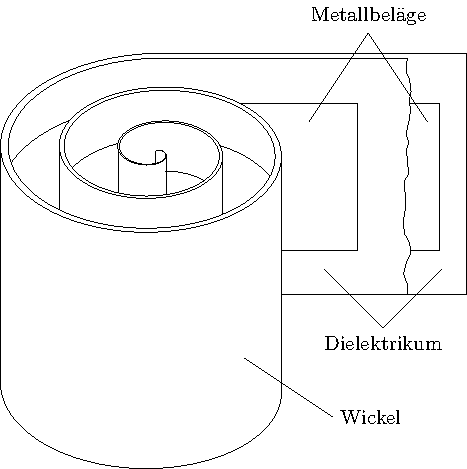
\includegraphics[width=1.0\linewidth]{img/49.pdf}}\end{PQuestion}

}
\only<2>{
\begin{PQuestion}{EB103}{An den Metallbelägen eines Wickelkondensators mit \qty{0,15}{\mm} starkem Kunststoff-Dielektrikum liegt eine Spannung von \qty{300}{\V}. Wie hoch ist die elektrische Feldstärke zwischen den Metallbelägen ungefähr?}{\qty{2000}{\V}/m}
{\qty{200}{\V}/m}
{\textbf{\textcolor{DARCgreen}{\qty{2000}{\kV}/m}}}
{\qty{200}{\kV}/m}
{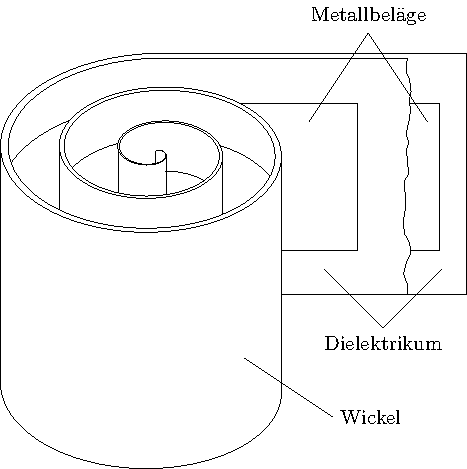
\includegraphics[width=1.0\linewidth]{img/49.pdf}}\end{PQuestion}

}
\end{frame}

\begin{frame}
\only<1>{
\begin{QQuestion}{EB104}{Ein Kondensator in einer Senderendstufe hat eine \qty{0,15}{\mm} starke PTFE-Folie als Dielektrikum. Die Durchschlagsfestigkeit von PTFE beträgt ca. \qty{400}{\kV}/cm. Wie groß wäre die maximale Spannung, die an den Kondensator angelegt werden kann, ohne dass die Folie durchschlagen wird?}{\qty{26}{\V}}
{\qty{60}{\kV}}
{\qty{6}{\kV}}
{\qty{2,6}{\kV}}
\end{QQuestion}

}
\only<2>{
\begin{QQuestion}{EB104}{Ein Kondensator in einer Senderendstufe hat eine \qty{0,15}{\mm} starke PTFE-Folie als Dielektrikum. Die Durchschlagsfestigkeit von PTFE beträgt ca. \qty{400}{\kV}/cm. Wie groß wäre die maximale Spannung, die an den Kondensator angelegt werden kann, ohne dass die Folie durchschlagen wird?}{\qty{26}{\V}}
{\qty{60}{\kV}}
{\textbf{\textcolor{DARCgreen}{\qty{6}{\kV}}}}
{\qty{2,6}{\kV}}
\end{QQuestion}

}
\end{frame}

\begin{frame}
\frametitle{Lösungsweg}
Der Trick ist hier, dass die Durschlagsfestigkeit die elektrische Feldstärke $E$ ist.

\begin{itemize}
  \item Gegeben: $d = 0,15mm$ und $E = 400\frac{kV}{cm}$
  \item Gesucht: $U$
  \item Lösung:
  \end{itemize}
$E = \frac{U}{d} \Rightarrow U = E\cdot d$

$U = 400\cdot\frac{10^3V}{10^{-2}m}\cdot 0,15\cdot 10^{-3}m$

$U = 6\cdot10^3V = 6kV$

\end{frame}

\begin{frame}
\frametitle{Vertikalantenne}
\begin{columns}
    \begin{column}{0.48\textwidth}
    \begin{itemize}
  \item An einer Antenne entstehen ebenso elektrische Feldlinien
  \item Die Feldlinien einer Vertikalantenne verlaufen vom \enquote{positiven Ende} zur Erde
  \end{itemize}

    \end{column}
   \begin{column}{0.48\textwidth}
       
\begin{figure}
    \DARCimage{0.85\linewidth}{193include}
    \caption{\scriptsize Feldlinien an einer Vertikalantenne}
    \label{e_feldlinien_vertikalantenne}
\end{figure}


   \end{column}
\end{columns}

\end{frame}

\begin{frame}
\only<1>{
\begin{PQuestion}{EB105}{Wie werden die mit X gekennzeichneten Feldlinien einer Vertikalantenne bezeichnet?}{Radiale Feldlinien}
{Magnetische Feldlinien}
{Elektrische Feldlinien}
{Horizontale Feldlinien}
{\DARCimage{1.0\linewidth}{193include}}\end{PQuestion}

}
\only<2>{
\begin{PQuestion}{EB105}{Wie werden die mit X gekennzeichneten Feldlinien einer Vertikalantenne bezeichnet?}{Radiale Feldlinien}
{Magnetische Feldlinien}
{\textbf{\textcolor{DARCgreen}{Elektrische Feldlinien}}}
{Horizontale Feldlinien}
{\DARCimage{1.0\linewidth}{193include}}\end{PQuestion}

}
\end{frame}%ENDCONTENT


\section{Magnetisches Feld}
\label{section:h_feld}
\begin{frame}%STARTCONTENT

\frametitle{Stromdurchflossener Leiter}
\begin{columns}
    \begin{column}{0.48\textwidth}
    \begin{itemize}
  \item Fließt Strom durch einen Leiter, bilden sich konzentrische, magnetische Felder um den Leiter
  \end{itemize}

    \end{column}
   \begin{column}{0.48\textwidth}
       Grafik eines stromdurchflossenen Leiters mit konzentrischen magnetischen Feldlinien kommt noch


   \end{column}
\end{columns}

\end{frame}

\begin{frame}
\only<1>{
\begin{QQuestion}{EB201}{Wenn ein konstanter Gleichstrom durch einen gestreckten Leiter fließt, sind die~...}{magnetischen Feldlinien sternförmig um den Leiter.}
{elektrischen Feldlinien konzentrische Kreise um den Leiter.}
{magnetischen Feldlinien konzentrische Kreise um den Leiter.}
{elektrischen Feldlinien parallel zu den magnetischen Feldlinien um den Leiter.}
\end{QQuestion}

}
\only<2>{
\begin{QQuestion}{EB201}{Wenn ein konstanter Gleichstrom durch einen gestreckten Leiter fließt, sind die~...}{magnetischen Feldlinien sternförmig um den Leiter.}
{elektrischen Feldlinien konzentrische Kreise um den Leiter.}
{\textbf{\textcolor{DARCgreen}{magnetischen Feldlinien konzentrische Kreise um den Leiter.}}}
{elektrischen Feldlinien parallel zu den magnetischen Feldlinien um den Leiter.}
\end{QQuestion}

}
\end{frame}

\begin{frame}
\frametitle{Homogenes magnetisches Feld}
\begin{columns}
    \begin{column}{0.48\textwidth}
    \begin{itemize}
  \item Wird ein stromdurchflossener Leiter zu einer Zylinderspule aufgewickelt, entsteht im inneren ein homogenes magnetisches Feld (\emph{H-Feld})
  \item Eine Spule speichert magnetische Energie
  \end{itemize}

    \end{column}
   \begin{column}{0.48\textwidth}
       
\begin{figure}
    \DARCimage{0.85\linewidth}{50include}
    \caption{\scriptsize Magnetische Feldlinien in einer Zylinderspule}
    \label{e_h_feld_spule}
\end{figure}

\begin{itemize}
  \item Einheit: $\dfrac{A}{m}$
  \end{itemize}

   \end{column}
\end{columns}

\end{frame}

\begin{frame}
\only<1>{
\begin{PQuestion}{EB202}{Welches Feld stellt sich im Inneren einer langen Zylinderspule bei Fließen eines Gleichstroms näherungsweise ein?}{Homogenes magnetisches Feld}
{Homogenes elektrisches Feld}
{Konzentrisches magnetisches Feld}
{Zentriertes magnetisches Feld}
{\DARCimage{1.0\linewidth}{50include}}\end{PQuestion}

}
\only<2>{
\begin{PQuestion}{EB202}{Welches Feld stellt sich im Inneren einer langen Zylinderspule bei Fließen eines Gleichstroms näherungsweise ein?}{\textbf{\textcolor{DARCgreen}{Homogenes magnetisches Feld}}}
{Homogenes elektrisches Feld}
{Konzentrisches magnetisches Feld}
{Zentriertes magnetisches Feld}
{\DARCimage{1.0\linewidth}{50include}}\end{PQuestion}

}
\end{frame}

\begin{frame}
\only<1>{
\begin{QQuestion}{EA104}{Welche Einheit wird üblicherweise für die magnetische Feldstärke verwendet?}{Ampere pro Meter (A/m)}
{Watt pro Meter (W/m)}
{Volt pro Meter (V/m)}
{Henry pro Meter (H/m)}
\end{QQuestion}

}
\only<2>{
\begin{QQuestion}{EA104}{Welche Einheit wird üblicherweise für die magnetische Feldstärke verwendet?}{\textbf{\textcolor{DARCgreen}{Ampere pro Meter (A/m)}}}
{Watt pro Meter (W/m)}
{Volt pro Meter (V/m)}
{Henry pro Meter (H/m)}
\end{QQuestion}

}
\end{frame}

\begin{frame}
\frametitle{Ringkern}
\begin{columns}
    \begin{column}{0.48\textwidth}
    \begin{itemize}
  \item Leiter wird auf einen magnetisch leitenden Ringkern gewickelt, z.B. Eisen
  \item Vorteile: Platzsparend und stabiler
  \end{itemize}

    \end{column}
   \begin{column}{0.48\textwidth}
       
\begin{figure}
    \DARCimage{0.85\linewidth}{40include}
    \caption{\scriptsize Ringkernspule}
    \label{e_ringkern}
\end{figure}


   \end{column}
\end{columns}

\end{frame}

\begin{frame}
\begin{columns}
    \begin{column}{0.48\textwidth}
    \begin{itemize}
  \item Magnetische Feldstärke $H = \dfrac{I\cdot N}{l_m}$ in $\dfrac{A}{m}$
  \item mit $N$ als Wicklungsanzahl und $l_m$ mittlere Länge des Rings
  \end{itemize}

    \end{column}
   \begin{column}{0.48\textwidth}
       
\begin{figure}
    \DARCimage{0.85\linewidth}{40include}
    \caption{\scriptsize Ringkernspule}
    \label{e_ringkern}
\end{figure}


   \end{column}
\end{columns}

\end{frame}

\begin{frame}
\only<1>{
\begin{PQuestion}{EB203}{Ein Ringkern hat einen mittleren Durchmesser von \qty{2,6}{\cm} und trägt 6 Windungen Kupferdraht. Wie groß ist die mittlere magnetische Feldstärke im Ringkern, wenn der Strom \qty{2,5}{\A} beträgt?}{\qty{183,6}{\A}/m}
{\qty{1,836}{\A}/m}
{\qty{5769}{\A}/m}
{\qty{5,769}{\A}/m}
{\DARCimage{0.5\linewidth}{40include}}\end{PQuestion}

}
\only<2>{
\begin{PQuestion}{EB203}{Ein Ringkern hat einen mittleren Durchmesser von \qty{2,6}{\cm} und trägt 6 Windungen Kupferdraht. Wie groß ist die mittlere magnetische Feldstärke im Ringkern, wenn der Strom \qty{2,5}{\A} beträgt?}{\textbf{\textcolor{DARCgreen}{\qty{183,6}{\A}/m}}}
{\qty{1,836}{\A}/m}
{\qty{5769}{\A}/m}
{\qty{5,769}{\A}/m}
{\DARCimage{0.5\linewidth}{40include}}\end{PQuestion}

}

\end{frame}

\begin{frame}
\only<1>{
\begin{QQuestion}{EB204}{Welcher der nachfolgenden Werkstoffe ist bei Raumtemperatur ein ferromagnetischer Stoff?}{Kupfer}
{Chrom}
{Eisen}
{Aluminium}
\end{QQuestion}

}
\only<2>{
\begin{QQuestion}{EB204}{Welcher der nachfolgenden Werkstoffe ist bei Raumtemperatur ein ferromagnetischer Stoff?}{Kupfer}
{Chrom}
{\textbf{\textcolor{DARCgreen}{Eisen}}}
{Aluminium}
\end{QQuestion}

}
\end{frame}

\begin{frame}
\frametitle{Magnetfeld einer Antenne}
\begin{columns}
    \begin{column}{0.48\textwidth}
    \begin{itemize}
  \item An einer Antenne wirkt das Magnetfeld um den Leiter
  \item Hier an einer Vertikalantenne konzentrisch um die Antenne
  \end{itemize}

    \end{column}
   \begin{column}{0.48\textwidth}
       
\begin{figure}
    \DARCimage{0.85\linewidth}{192include}
    \caption{\scriptsize Magnetfeld an einer Vertikalantenne}
    \label{e_vertikalantenne_magnetfeld}
\end{figure}


   \end{column}
\end{columns}

\end{frame}

\begin{frame}
\only<1>{
\begin{PQuestion}{EB206}{Wie werden die mit X gekennzeichneten Feldlinien einer Vertikalantenne bezeichnet?}{Offene Feldlinien}
{Elektrische Feldlinien}
{Magnetische Feldlinien}
{Vertikale Feldlinien}
{\DARCimage{1.0\linewidth}{192include}}\end{PQuestion}

}
\only<2>{
\begin{PQuestion}{EB206}{Wie werden die mit X gekennzeichneten Feldlinien einer Vertikalantenne bezeichnet?}{Offene Feldlinien}
{Elektrische Feldlinien}
{\textbf{\textcolor{DARCgreen}{Magnetische Feldlinien}}}
{Vertikale Feldlinien}
{\DARCimage{1.0\linewidth}{192include}}\end{PQuestion}

}
\end{frame}%ENDCONTENT


\section{Elektromagnetisches Feld}
\label{section:em_feld}
\begin{frame}%STARTCONTENT

\begin{columns}
    \begin{column}{0.48\textwidth}
    \begin{itemize}
  \item Fließt ein zeitlich veränderlicher Strom durch einen Leiter, z.B. eine Antenne, entsteht sowohl ein elektrisches als auch ein magnetisches Feld
  \item Dieses wird als elektromagnetisches Feld bezeichnet
  \item Die beiden Felder stehen in einem 90º-Winkel zueinander
  \end{itemize}

    \end{column}
   \begin{column}{0.48\textwidth}
       
\begin{figure}
    \DARCimage{0.85\linewidth}{192include}
    \caption{\scriptsize Elektrisches und magnetisches Feld an einer Antenne}
    \label{e_vertikalantenne_magnetfeld}
\end{figure}


   \end{column}
\end{columns}

\end{frame}

\begin{frame}
\only<1>{
\begin{QQuestion}{EB301}{Wodurch entsteht ein elektromagnetisches Feld beispielsweise?}{Ein elektromagnetisches Feld entsteht, wenn ein zeitlich konstanter Strom durch einen elektrischen Leiter fließt.}
{Ein elektromagnetisches Feld entsteht, wenn ein zeitlich veränderlicher Strom durch einen elektrischen Leiter fließt.}
{Ein elektromagnetisches Feld entsteht, wenn eine zeitlich konstante Spannung an einem elektrischen Leiter anliegt.}
{Ein elektromagnetisches Feld entsteht, wenn eine zeitlich konstante Spannung an einem elektrischen Isolator anliegt.}
\end{QQuestion}

}
\only<2>{
\begin{QQuestion}{EB301}{Wodurch entsteht ein elektromagnetisches Feld beispielsweise?}{Ein elektromagnetisches Feld entsteht, wenn ein zeitlich konstanter Strom durch einen elektrischen Leiter fließt.}
{\textbf{\textcolor{DARCgreen}{Ein elektromagnetisches Feld entsteht, wenn ein zeitlich veränderlicher Strom durch einen elektrischen Leiter fließt.}}}
{Ein elektromagnetisches Feld entsteht, wenn eine zeitlich konstante Spannung an einem elektrischen Leiter anliegt.}
{Ein elektromagnetisches Feld entsteht, wenn eine zeitlich konstante Spannung an einem elektrischen Isolator anliegt.}
\end{QQuestion}

}
\end{frame}

\begin{frame}
\only<1>{
\begin{QQuestion}{EB302}{Wie erfolgt die Ausbreitung einer elektromagnetischen Welle? Die Ausbreitung erfolgt~...}{nur über das magnetische Feld. Das elektrische Feld wirkt sich nur im Nahfeld aus.}
{nur über das elektrische Feld. Das magnetische Feld wirkt sich nur im Nahfeld aus.}
{durch eine Wechselwirkung zwischen elektrischem und magnetischem Feld.}
{durch die unabhängige Ausbreitung von elektrischem und magnetischem Feld.}
\end{QQuestion}

}
\only<2>{
\begin{QQuestion}{EB302}{Wie erfolgt die Ausbreitung einer elektromagnetischen Welle? Die Ausbreitung erfolgt~...}{nur über das magnetische Feld. Das elektrische Feld wirkt sich nur im Nahfeld aus.}
{nur über das elektrische Feld. Das magnetische Feld wirkt sich nur im Nahfeld aus.}
{\textbf{\textcolor{DARCgreen}{durch eine Wechselwirkung zwischen elektrischem und magnetischem Feld.}}}
{durch die unabhängige Ausbreitung von elektrischem und magnetischem Feld.}
\end{QQuestion}

}
\end{frame}

\begin{frame}
\only<1>{
\begin{QQuestion}{EB303}{Der Winkel zwischen den elektrischen und magnetischen Feldkomponenten eines elektromagnetischen Feldes beträgt bei Freiraumausbreitung im Fernfeld~...}{\qty{90}{\degree}.}
{\qty{45}{\degree}.}
{\qty{180}{\degree}.}
{\qty{360}{\degree}.}
\end{QQuestion}

}
\only<2>{
\begin{QQuestion}{EB303}{Der Winkel zwischen den elektrischen und magnetischen Feldkomponenten eines elektromagnetischen Feldes beträgt bei Freiraumausbreitung im Fernfeld~...}{\textbf{\textcolor{DARCgreen}{\qty{90}{\degree}.}}}
{\qty{45}{\degree}.}
{\qty{180}{\degree}.}
{\qty{360}{\degree}.}
\end{QQuestion}

}
\end{frame}

\begin{frame}
\only<1>{
\begin{QQuestion}{EB304}{Welche Aussage trifft auf die elektromagnetische Ausstrahlung im ungestörten Fernfeld zu?}{Die E-Feldkomponente und die H-Feldkomponente sind phasengleich und sind parallel zueinander. Die Ausbreitungsrichtung verläuft dazu in einem rechten Winkel.}
{Die E-Feldkomponente und die H-Feldkomponente stehen in einem rechten Winkel zueinander. Die Ausbreitungsrichtung hat keine feste Beziehung dazu.}
{Die E-Feldkomponente, die H-Feldkomponente und die Ausbreitungsrichtung stehen in einem rechten Winkel zueinander.}
{Die Ausbreitungsrichtung befindet sich parallel zur E-Feldkomponente und verläuft senkrecht zur H-Feldkomponente.}
\end{QQuestion}

}
\only<2>{
\begin{QQuestion}{EB304}{Welche Aussage trifft auf die elektromagnetische Ausstrahlung im ungestörten Fernfeld zu?}{Die E-Feldkomponente und die H-Feldkomponente sind phasengleich und sind parallel zueinander. Die Ausbreitungsrichtung verläuft dazu in einem rechten Winkel.}
{Die E-Feldkomponente und die H-Feldkomponente stehen in einem rechten Winkel zueinander. Die Ausbreitungsrichtung hat keine feste Beziehung dazu.}
{\textbf{\textcolor{DARCgreen}{Die E-Feldkomponente, die H-Feldkomponente und die Ausbreitungsrichtung stehen in einem rechten Winkel zueinander.}}}
{Die Ausbreitungsrichtung befindet sich parallel zur E-Feldkomponente und verläuft senkrecht zur H-Feldkomponente.}
\end{QQuestion}

}
\end{frame}%ENDCONTENT


\section{Polarisation elektromagnetischer Wellen}
\label{section:em_feld_polarisation}
\begin{frame}%STARTCONTENT

\frametitle{Horizontale Polarisation}
\begin{columns}
    \begin{column}{0.48\textwidth}
    \begin{itemize}
  \item Die Lage des E-Feldes gibt die Polarisation an
  \item Breitet sich das E-Feld horizontal aus, wird von horizontaler Polarisation gesprochen
  \item Ist von Bauform der Antenne abhängig
  \end{itemize}

    \end{column}
   \begin{column}{0.48\textwidth}
       
\begin{figure}
    \DARCimage{0.85\linewidth}{194include}
    \caption{\scriptsize Horizontale Polarisation in einem Feld}
    \label{e_horizontale_polarisation}
\end{figure}


   \end{column}
\end{columns}

\end{frame}

\begin{frame}
\only<1>{
\begin{QQuestion}{EB305}{Die Polarisation einer elektromagnetischen Welle ist durch die Richtung~...}{der Ausbreitung (S-Vektor/Poynting-Vektor) bestimmt.}
{des magnetischen Nordpols (relativ zur Antenne) bestimmt.}
{des elektrischen Feldes (Vektor des E-Feldes) bestimmt.}
{des unmittelbaren Nahfeldes ($\lambda/4$-Bereich) bestimmt.}
\end{QQuestion}

}
\only<2>{
\begin{QQuestion}{EB305}{Die Polarisation einer elektromagnetischen Welle ist durch die Richtung~...}{der Ausbreitung (S-Vektor/Poynting-Vektor) bestimmt.}
{des magnetischen Nordpols (relativ zur Antenne) bestimmt.}
{\textbf{\textcolor{DARCgreen}{des elektrischen Feldes (Vektor des E-Feldes) bestimmt.}}}
{des unmittelbaren Nahfeldes ($\lambda/4$-Bereich) bestimmt.}
\end{QQuestion}

}
\end{frame}

\begin{frame}
\only<1>{
\begin{PQuestion}{EB306}{Das folgende Bild zeigt eine Momentaufnahme eines elektromagnetischen Feldes. Welche Polarisation hat die skizzierte Welle?}{Rechtszirkulare Polarisation}
{Vertikale Polarisation}
{Horizontale Polarisation}
{Linkszirkulare Polarisation}
{\DARCimage{1.0\linewidth}{194include}}\end{PQuestion}

}
\only<2>{
\begin{PQuestion}{EB306}{Das folgende Bild zeigt eine Momentaufnahme eines elektromagnetischen Feldes. Welche Polarisation hat die skizzierte Welle?}{Rechtszirkulare Polarisation}
{Vertikale Polarisation}
{\textbf{\textcolor{DARCgreen}{Horizontale Polarisation}}}
{Linkszirkulare Polarisation}
{\DARCimage{1.0\linewidth}{194include}}\end{PQuestion}

}
\end{frame}

\begin{frame}
\only<1>{
\begin{PQuestion}{EB309}{Die Polarisation des Sendesignals in der Hauptstrahlrichtung dieser Richtantenne ist~...}{linksdrehend.}
{vertikal.}
{rechtsdrehend.}
{horizontal.}
{\DARCimage{1.0\linewidth}{326include}}\end{PQuestion}

}
\only<2>{
\begin{PQuestion}{EB309}{Die Polarisation des Sendesignals in der Hauptstrahlrichtung dieser Richtantenne ist~...}{linksdrehend.}
{vertikal.}
{rechtsdrehend.}
{\textbf{\textcolor{DARCgreen}{horizontal.}}}
{\DARCimage{1.0\linewidth}{326include}}\end{PQuestion}

}
\end{frame}

\begin{frame}
\frametitle{Vertikale Polarisation}
\begin{columns}
    \begin{column}{0.48\textwidth}
    \begin{itemize}
  \item Die Lage des E-Feldes gibt die Polarisation an
  \item Breitet sich das E-Feld vertikal aus, wird von vertikaler Polarisation gesprochen
  \item Ist von Bauform der Antenne abhängig
  \end{itemize}

    \end{column}
   \begin{column}{0.48\textwidth}
       
\begin{figure}
    \DARCimage{0.85\linewidth}{203include}
    \caption{\scriptsize Vertikale Polarisation in einem Feld}
    \label{e_vertikale_polarisation}
\end{figure}


   \end{column}
\end{columns}

\end{frame}

\begin{frame}
\only<1>{
\begin{PQuestion}{EB307}{Das folgende Bild zeigt eine Momentaufnahme eines elektromagnetischen Feldes. Welche Polarisation hat die skizzierte Welle?}{Vertikale Polarisation}
{Horizontale Polarisation}
{Linkszirkulare Polarisation}
{Rechtszirkulare Polarisation}
{\DARCimage{1.0\linewidth}{203include}}\end{PQuestion}

}
\only<2>{
\begin{PQuestion}{EB307}{Das folgende Bild zeigt eine Momentaufnahme eines elektromagnetischen Feldes. Welche Polarisation hat die skizzierte Welle?}{\textbf{\textcolor{DARCgreen}{Vertikale Polarisation}}}
{Horizontale Polarisation}
{Linkszirkulare Polarisation}
{Rechtszirkulare Polarisation}
{\DARCimage{1.0\linewidth}{203include}}\end{PQuestion}

}
\end{frame}

\begin{frame}
\only<1>{
\begin{PQuestion}{EB310}{Die Polarisation des Sendesignals in der Hauptstrahlrichtung dieser Richtantenne ist~...}{horizontal.}
{vertikal.}
{rechtsdrehend.}
{linksdrehend.}
{\DARCimage{1.0\linewidth}{51include}}\end{PQuestion}

}
\only<2>{
\begin{PQuestion}{EB310}{Die Polarisation des Sendesignals in der Hauptstrahlrichtung dieser Richtantenne ist~...}{horizontal.}
{\textbf{\textcolor{DARCgreen}{vertikal.}}}
{rechtsdrehend.}
{linksdrehend.}
{\DARCimage{1.0\linewidth}{51include}}\end{PQuestion}

}
\end{frame}

\begin{frame}
\frametitle{Zirkulare Polarisation}
\begin{columns}
    \begin{column}{0.48\textwidth}
    \begin{itemize}
  \item Die Lage des E-Feldes gibt die Polarisation an
  \item Breitet sich das E-Feld zirkular aus, wird von zirkularer Polarisation gesprochen
  \item Es ist rechts- und linksdrehend möglich
  \item Ist von Bauform der Antenne abhängig
  \end{itemize}

    \end{column}
   \begin{column}{0.48\textwidth}
       
\begin{figure}
    \DARCimage{0.85\linewidth}{204include}
    \caption{\scriptsize Zirkulare Polarisation in einem Feld}
    \label{e_zirkulare_polarisation}
\end{figure}


   \end{column}
\end{columns}

\end{frame}

\begin{frame}
\only<1>{
\begin{PQuestion}{EB308}{Das folgende Bild zeigt eine Momentaufnahme eines elektromagnetischen Feldes. Welche Polarisation hat die skizzierte Welle?}{Zirkulare Polarisation}
{Horizontale Polarisation}
{Vertikale Polarisation}
{Diagonale Polarisation}
{\DARCimage{1.0\linewidth}{204include}}\end{PQuestion}

}
\only<2>{
\begin{PQuestion}{EB308}{Das folgende Bild zeigt eine Momentaufnahme eines elektromagnetischen Feldes. Welche Polarisation hat die skizzierte Welle?}{\textbf{\textcolor{DARCgreen}{Zirkulare Polarisation}}}
{Horizontale Polarisation}
{Vertikale Polarisation}
{Diagonale Polarisation}
{\DARCimage{1.0\linewidth}{204include}}\end{PQuestion}

}
\end{frame}%ENDCONTENT


\title{DARC Amateurfunklehrgang Klasse E}
\author{Bauelemente}
\institute{Deutscher Amateur Radio Club e.\,V.}
\begin{frame}
\maketitle
\end{frame}

\section{Kondensator I}
\label{section:kondensator_1}
\begin{frame}%STARTCONTENT

\frametitle{Kapazität}
\begin{itemize}
  \item Wichtigste Eigenschaft des Kondensators: Ladung speichern
  \item $\rightarrow$ Kapazität
  \end{itemize}
$C = \dfrac{Q}{U}$

\begin{itemize}
  \item mit $Q$ als elektrische Ladung
  \item Einheit: $\frac{As}{V}$ bzw. Farad $F$
  \item Die Kapazität ist die elektrische Ladung pro Volt
  \end{itemize}

\end{frame}

\begin{frame}
\frametitle{Kapazität durch Bauart}
\begin{columns}
    \begin{column}{0.48\textwidth}
    \begin{itemize}
  \item Die Kapazität kann durch die Bauart erreicht werden
  \end{itemize}
$C = \dfrac{\varepsilon_0 \cdot \varepsilon_r \cdot A}{d}$

\begin{itemize}
  \item $\rightarrow$ Kapazität ist größer bei größerer Fläche, kleinem Abstand oder anderem Dielektrikum
  \end{itemize}

    \end{column}
   \begin{column}{0.48\textwidth}
       \begin{itemize}
  \item $\varepsilon_0 = 0,855 \cdot 10^{-11}\frac{As}{Vm}$: elektrische Feldkonstante
  \item $\varepsilon_r$: relative Dielektrizitätszahl, abhängig vom Dielektrikum (ohne Einheit)
  \item $A$: Fläche der Kondensatorplatten
  \item $d$: Abstand der Platten
  \end{itemize}

   \end{column}
\end{columns}

\end{frame}

\begin{frame}
\only<1>{
\begin{QQuestion}{EA101}{Welche Einheit wird üblicherweise für die Kapazität verwendet?}{Amperestunden (Ah)}
{Ohm ($\Omega$)}
{Farad (F)}
{Henry (H)}
\end{QQuestion}

}
\only<2>{
\begin{QQuestion}{EA101}{Welche Einheit wird üblicherweise für die Kapazität verwendet?}{Amperestunden (Ah)}
{Ohm ($\Omega$)}
{\textbf{\textcolor{DARCgreen}{Farad (F)}}}
{Henry (H)}
\end{QQuestion}

}
\end{frame}

\begin{frame}
\only<1>{
\begin{QQuestion}{EC205}{Von welcher der nachfolgenden Größen ist die Kapazität eines Plattenkondensators \underline{nicht} abhängig?}{Plattenabstand}
{Spannung}
{Plattenfläche}
{Dielektrikum}
\end{QQuestion}

}
\only<2>{
\begin{QQuestion}{EC205}{Von welcher der nachfolgenden Größen ist die Kapazität eines Plattenkondensators \underline{nicht} abhängig?}{Plattenabstand}
{\textbf{\textcolor{DARCgreen}{Spannung}}}
{Plattenfläche}
{Dielektrikum}
\end{QQuestion}

}
\end{frame}

\begin{frame}
\only<1>{
\begin{QQuestion}{EC203}{Wodurch verringert sich die Kapazität eines Plattenkondensators? Durch~...}{eine größere Dielektrizitätskonstante des Dielektrikums.}
{einen größeren Plattenabstand.}
{eine größere Spannung.}
{größere Plattenflächen.}
\end{QQuestion}

}
\only<2>{
\begin{QQuestion}{EC203}{Wodurch verringert sich die Kapazität eines Plattenkondensators? Durch~...}{eine größere Dielektrizitätskonstante des Dielektrikums.}
{\textbf{\textcolor{DARCgreen}{einen größeren Plattenabstand.}}}
{eine größere Spannung.}
{größere Plattenflächen.}
\end{QQuestion}

}
\end{frame}

\begin{frame}
\only<1>{
\begin{QQuestion}{EC204}{In welchem Fall sinkt die Kapazität eines Plattenkondensators?}{Bei Vergrößerung der Plattenoberfläche}
{Bei Erhöhung der angelegten Spannung}
{Bei Vergrößerung des Plattenabstandes}
{Bei Vergrößerung der Dielektrizitätszahl}
\end{QQuestion}

}
\only<2>{
\begin{QQuestion}{EC204}{In welchem Fall sinkt die Kapazität eines Plattenkondensators?}{Bei Vergrößerung der Plattenoberfläche}
{Bei Erhöhung der angelegten Spannung}
{\textbf{\textcolor{DARCgreen}{Bei Vergrößerung des Plattenabstandes}}}
{Bei Vergrößerung der Dielektrizitätszahl}
\end{QQuestion}

}
\end{frame}

\begin{frame}
\frametitle{Drehkondensator}
\begin{columns}
    \begin{column}{0.48\textwidth}
    \begin{itemize}
  \item Eine Platte ist feststehend, die andere Platte kann rotiert werden
  \item Nur dort, wo die Platten sich überlappen, wirkt der Kondensator
  \item Die Fläche wird durch Drehung verändert $\rightarrow$ Änderung der Kapazität
  \end{itemize}

    \end{column}
   \begin{column}{0.48\textwidth}
       
\begin{figure}
    \DARCimage{0.85\linewidth}{840include}
    \caption{\scriptsize Drehkondensator}
    \label{e_kondensator_drehkondensator}
\end{figure}


   \end{column}
\end{columns}

\end{frame}

\begin{frame}
\only<1>{
\begin{QQuestion}{EC206}{Wie nennt man ein Bauelement, bei dem sich Platten auf einer isolierten Achse befinden, die zwischen fest stehenden Platten rotiert werden können?}{Drehkondensator}
{Styroflexkondensator}
{Keramischer Kondensator}
{Rotorkondensator}
\end{QQuestion}

}
\only<2>{
\begin{QQuestion}{EC206}{Wie nennt man ein Bauelement, bei dem sich Platten auf einer isolierten Achse befinden, die zwischen fest stehenden Platten rotiert werden können?}{\textbf{\textcolor{DARCgreen}{Drehkondensator}}}
{Styroflexkondensator}
{Keramischer Kondensator}
{Rotorkondensator}
\end{QQuestion}

}
\end{frame}

\begin{frame}
\frametitle{Elektrolytkondensator}
\begin{columns}
    \begin{column}{0.48\textwidth}
    \begin{itemize}
  \item Spezielle Bauform
  \item Ermöglicht große Kapazität
  \item Nur für Gleichspannung
  \item Polarität muss beachtet werden
  \end{itemize}

    \end{column}
   \begin{column}{0.48\textwidth}
       
\begin{figure}
    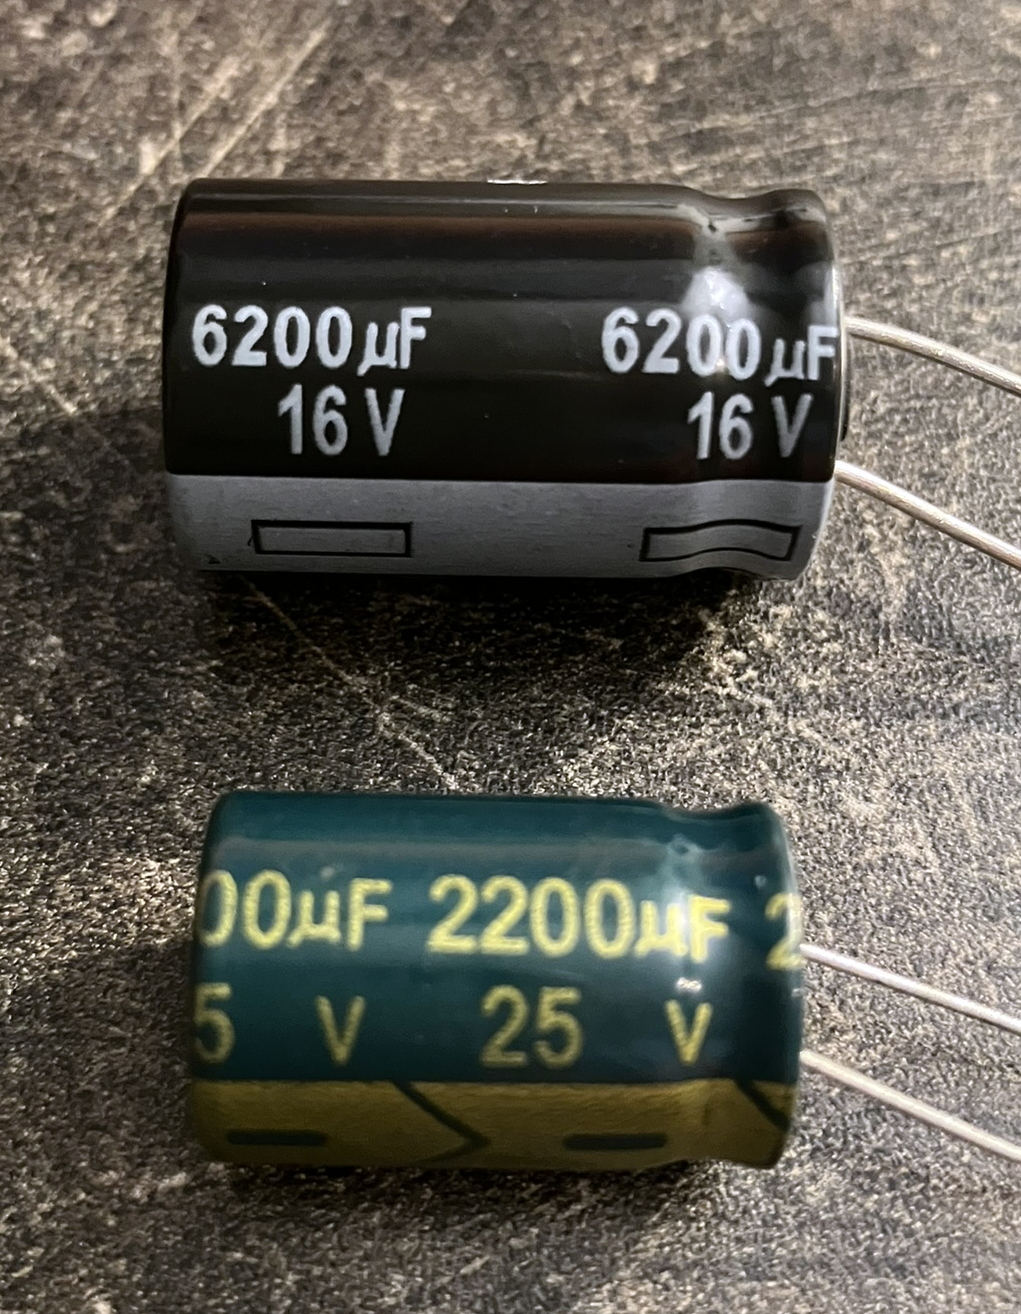
\includegraphics[width=0.85\textwidth]{foto/198}
    \caption{\scriptsize Elektrolytkondensatoren mit Markierung des Minus-Pols}
    \label{e_kondensator_elkos}
\end{figure}

   \end{column}
\end{columns}

\end{frame}

\begin{frame}
\only<1>{
\begin{QQuestion}{EC207}{Bei welcher der folgenden Bauformen von Kondensatoren muss beim Einbau auf die Polarität geachtet werden?}{Elektrolytkondensator}
{Keramikkondensator}
{Styroflexkondensator}
{Plattenkondensator}
\end{QQuestion}

}
\only<2>{
\begin{QQuestion}{EC207}{Bei welcher der folgenden Bauformen von Kondensatoren muss beim Einbau auf die Polarität geachtet werden?}{\textbf{\textcolor{DARCgreen}{Elektrolytkondensator}}}
{Keramikkondensator}
{Styroflexkondensator}
{Plattenkondensator}
\end{QQuestion}

}
\end{frame}

\begin{frame}
\frametitle{Ladekurve}
\begin{columns}
    \begin{column}{0.48\textwidth}
    \begin{itemize}
  \item Ein leerer Kondensator wird an Gleichspannung angeschlossen
  \item Die Spannung steigt steil an und flacht dann zur angelegten Spannung ab 
  \end{itemize}

    \end{column}
   \begin{column}{0.48\textwidth}
       
\begin{figure}
    \DARCimage{0.85\linewidth}{185include}
    \caption{\scriptsize Ladekurve eines Kondensators}
    \label{e_ladekurve_kondensator}
\end{figure}


   \end{column}
\end{columns}

\end{frame}

\begin{frame}
\only<1>{
\begin{question2x2}{EC201}{Welchen zeitlichen Verlauf hat die Spannung an einem entladenen Kondensator, wenn dieser über einen Widerstand an eine Gleichspannungsquelle angeschlossen wird?}{\DARCimage{1.0\linewidth}{188include}}
{\DARCimage{1.0\linewidth}{186include}}
{\DARCimage{1.0\linewidth}{185include}}
{\DARCimage{1.0\linewidth}{187include}}
\end{question2x2}

}
\only<2>{
\begin{question2x2}{EC201}{Welchen zeitlichen Verlauf hat die Spannung an einem entladenen Kondensator, wenn dieser über einen Widerstand an eine Gleichspannungsquelle angeschlossen wird?}{\DARCimage{1.0\linewidth}{188include}}
{\DARCimage{1.0\linewidth}{186include}}
{\textbf{\textcolor{DARCgreen}{\DARCimage{1.0\linewidth}{185include}}}}
{\DARCimage{1.0\linewidth}{187include}}
\end{question2x2}

}
\end{frame}

\begin{frame}
\frametitle{Kondensator im Wechselstrom}
\begin{itemize}
  \item Im Gleichstromkreis lädt der Kondensator sich auf, wirkt dann aber wie ein unendlich großer Widerstand
  \item Bei Wechselstrom wird der Kondensator ständig Auf- und Entladen
  \item Je höher die Frequenz, umso geringer ist der Wechselstromwiderstand des Kondensators
  \end{itemize}
\end{frame}

\begin{frame}
\only<1>{
\begin{QQuestion}{EC202}{Welches Verhalten zeigt der Wechselstromwiderstand eines idealen Kondensators mit zunehmender Frequenz?}{Er sinkt.}
{Er sinkt bis zu einem Minimum und steigt dann wieder.}
{Er steigt.}
{Er steigt bis zu einem Maximum und sinkt dann wieder.}
\end{QQuestion}

}
\only<2>{
\begin{QQuestion}{EC202}{Welches Verhalten zeigt der Wechselstromwiderstand eines idealen Kondensators mit zunehmender Frequenz?}{\textbf{\textcolor{DARCgreen}{Er sinkt.}}}
{Er sinkt bis zu einem Minimum und steigt dann wieder.}
{Er steigt.}
{Er steigt bis zu einem Maximum und sinkt dann wieder.}
\end{QQuestion}

}
\end{frame}%ENDCONTENT


\section{Spule I}
\label{section:spule_1}
\begin{frame}%STARTCONTENT

\frametitle{Induktivität}
\begin{columns}
    \begin{column}{0.48\textwidth}
    \begin{itemize}
  \item Jeder stromdurchflossene Leiter hat eine Induktivität
  \item Um einen stromdurchflossenen Leiter entsteht ein Magnetfeld
  \item In einem Leiter entsteht ein Strom, wenn dieser durch ein Magnetfeld bewegt wird
  \end{itemize}

    \end{column}
   \begin{column}{0.48\textwidth}
       
\begin{figure}
    \DARCimage{0.85\linewidth}{833include}
    \caption{\scriptsize Magnetfeld um einen stromdurchflossenen Leiter}
    \label{e_spule_magnetfeld_um_leiter}
\end{figure}


   \end{column}
\end{columns}

\end{frame}

\begin{frame}
\only<1>{
\begin{QQuestion}{EC304}{Hat ein gerades Leiterstück eine Induktivität?}{Nein, der Leiter muss wenigstens eine Krümmung (eine viertel, halbe oder ganze Windung) haben.}
{Ja, jeder Leiter besitzt, unabhängig von der Form, eine Induktivität.}
{Ja, solange der Blindwiderstand \qty{0}{\ohm} beträgt.}
{Nein, beispielsweise im Vakuum entstehen keine Induktivitäten.}
\end{QQuestion}

}
\only<2>{
\begin{QQuestion}{EC304}{Hat ein gerades Leiterstück eine Induktivität?}{Nein, der Leiter muss wenigstens eine Krümmung (eine viertel, halbe oder ganze Windung) haben.}
{\textbf{\textcolor{DARCgreen}{Ja, jeder Leiter besitzt, unabhängig von der Form, eine Induktivität.}}}
{Ja, solange der Blindwiderstand \qty{0}{\ohm} beträgt.}
{Nein, beispielsweise im Vakuum entstehen keine Induktivitäten.}
\end{QQuestion}

}
\end{frame}

\begin{frame}
\frametitle{Spule und Induktivität}
\begin{itemize}
  \item Eine Spule optimiert die Induktivität eines Leiters
  \item Wichtigste Eigenschaft der Spule: Energie speichern
  \end{itemize}
$L = \dfrac{N\cdot \Phi}{I}$

\begin{itemize}
  \item mit $N$ Anzahl Windungen und $\Phi$ als magnetischer Fluss
  \item Einheit: $\frac{Vs}{A}$ bzw. Henry $H$
  \item Die Induktivität ist der magnetische Fluss pro Ampere
  \end{itemize}

\end{frame}

\begin{frame}
\frametitle{Induktivität durch Bauart}
\begin{columns}
    \begin{column}{0.48\textwidth}
    \begin{itemize}
  \item Die Induktivität einer Spule kann durch die Bauart erreicht werden
  \end{itemize}
$L = \dfrac{\mu_0 \cdot \mu_r \cdot N^2 \cdot A_S}{l}$

\begin{itemize}
  \item $\rightarrow$ Induktivität ist größer bei größerem Querschnitt, anderem Kern oder kleinerer Länge
  \item $\rightarrow$ Induktivität ist viel größer bei höherer Windungszahl
  \end{itemize}

    \end{column}
   \begin{column}{0.48\textwidth}
       \begin{itemize}
  \item $\mu_0 = 1,2566 \cdot 10^{-6}\frac{H}{m}$: magnetische Feldkonstante
  \item $\mu_r$: relative Permeabilität, abhängig vom Spulenkern (Luft  $\approx$  1)
  \item $N$: Windungszahl
  \item $A_S$: Querschnittsfläche der Spule
  \item $l$: Länge der Spule bzw. mittlere Feldlinienlänge
  \end{itemize}

   \end{column}
\end{columns}

\end{frame}

\begin{frame}
\only<1>{
\begin{QQuestion}{EA102}{Welche Einheit wird üblicherweise für die Induktivität verwendet?}{Henry (H)}
{Farad (F)}
{Ohm ($\Omega$)}
{Amperestunden (Ah)}
\end{QQuestion}

}
\only<2>{
\begin{QQuestion}{EA102}{Welche Einheit wird üblicherweise für die Induktivität verwendet?}{\textbf{\textcolor{DARCgreen}{Henry (H)}}}
{Farad (F)}
{Ohm ($\Omega$)}
{Amperestunden (Ah)}
\end{QQuestion}

}
\end{frame}

\begin{frame}
\only<1>{
\begin{PQuestion}{EC307}{Wie ändert sich die Induktivität einer Spule von \qty{12}{\micro\H}, wenn die Windungszahl bei gleicher Wickellänge verdoppelt wird?}{Die Induktivität steigt auf \qty{24}{\micro\H}.}
{Die Induktivität steigt auf \qty{48}{\micro\H}.}
{Die Induktivität sinkt auf \qty{6}{\micro\H}.}
{Die Induktivität sinkt auf \qty{3}{\micro\H}.}
{\DARCimage{1.0\linewidth}{449include}}\end{PQuestion}

}
\only<2>{
\begin{PQuestion}{EC307}{Wie ändert sich die Induktivität einer Spule von \qty{12}{\micro\H}, wenn die Windungszahl bei gleicher Wickellänge verdoppelt wird?}{Die Induktivität steigt auf \qty{24}{\micro\H}.}
{\textbf{\textcolor{DARCgreen}{Die Induktivität steigt auf \qty{48}{\micro\H}.}}}
{Die Induktivität sinkt auf \qty{6}{\micro\H}.}
{Die Induktivität sinkt auf \qty{3}{\micro\H}.}
{\DARCimage{1.0\linewidth}{449include}}\end{PQuestion}

}
\end{frame}

\begin{frame}
\only<1>{
\begin{PQuestion}{EC306}{Vorausgesetzt sind zwei Spulen in gleicher Umgebung, mit gleicher Windungszahl und mit gleicher Querschnittsfläche. Die erste Spule hat eine Induktivität von \qty{12}{\micro\H}. Die zweite Spule hat die doppelte Länge der ersten Spule. Wie hoch ist die Induktivität der zweiten Spule?}{\qty{3}{\micro\H}}
{\qty{24}{\micro\H}}
{\qty{48}{\micro\H}}
{\qty{6}{\micro\H}}
{\DARCimage{1.0\linewidth}{473include}}\end{PQuestion}

}
\only<2>{
\begin{PQuestion}{EC306}{Vorausgesetzt sind zwei Spulen in gleicher Umgebung, mit gleicher Windungszahl und mit gleicher Querschnittsfläche. Die erste Spule hat eine Induktivität von \qty{12}{\micro\H}. Die zweite Spule hat die doppelte Länge der ersten Spule. Wie hoch ist die Induktivität der zweiten Spule?}{\qty{3}{\micro\H}}
{\qty{24}{\micro\H}}
{\qty{48}{\micro\H}}
{\textbf{\textcolor{DARCgreen}{\qty{6}{\micro\H}}}}
{\DARCimage{1.0\linewidth}{473include}}\end{PQuestion}

}
\end{frame}

\begin{frame}
\only<1>{
\begin{QQuestion}{EC305}{Wie kann man die Induktivität einer zylindrischen Spule vergrößern?}{Durch Einführen eines Kupferkerns in die Spule.}
{Durch Auseinanderziehen der Spule in Längsrichtung.}
{Durch Stauchen der Spule in Längsrichtung.}
{Durch Einbau der Spule in einen Abschirmbecher.}
\end{QQuestion}

}
\only<2>{
\begin{QQuestion}{EC305}{Wie kann man die Induktivität einer zylindrischen Spule vergrößern?}{Durch Einführen eines Kupferkerns in die Spule.}
{Durch Auseinanderziehen der Spule in Längsrichtung.}
{\textbf{\textcolor{DARCgreen}{Durch Stauchen der Spule in Längsrichtung.}}}
{Durch Einbau der Spule in einen Abschirmbecher.}
\end{QQuestion}

}
\end{frame}

\begin{frame}
\frametitle{Stromfluss über eine Spule}
\begin{columns}
    \begin{column}{0.48\textwidth}
    \begin{itemize}
  \item Strom braucht länger durch die Spule
  \item Erst leuchtet Lampe<sub>1</sub>
  \item Später leuchtet Lampe<sub>2</sub>
  \end{itemize}

    \end{column}
   \begin{column}{0.48\textwidth}
       
\begin{figure}
    \DARCimage{0.85\linewidth}{541include}
    \caption{\scriptsize Stromkreis mit Spule}
    \label{e_stromkreis_mit_spule}
\end{figure}


   \end{column}
\end{columns}

\end{frame}

\begin{frame}
\only<1>{
\begin{PQuestion}{EC302}{Schaltet man zwei Leuchtmittel gleichzeitig an eine Gleichspannungsquelle, wobei ein Leuchtmittel, Lampe 1, zum Helligkeitsausgleich über einen Widerstand und das andere, Lampe 2, über eine Spule mit vielen Windungen und Eisenkern angeschlossen ist, so~...}{leuchtet Lampe 2 zuerst.}
{leuchtet Lampe 1 zuerst.}
{leuchten Lampe 1 und Lampe 2 genau gleichzeitig.}
{leuchtet Lampe 2 kurz auf und geht wieder aus. Lampe 1 leuchtet.}
{\DARCimage{1.0\linewidth}{541include}}\end{PQuestion}

}
\only<2>{
\begin{PQuestion}{EC302}{Schaltet man zwei Leuchtmittel gleichzeitig an eine Gleichspannungsquelle, wobei ein Leuchtmittel, Lampe 1, zum Helligkeitsausgleich über einen Widerstand und das andere, Lampe 2, über eine Spule mit vielen Windungen und Eisenkern angeschlossen ist, so~...}{leuchtet Lampe 2 zuerst.}
{\textbf{\textcolor{DARCgreen}{leuchtet Lampe 1 zuerst.}}}
{leuchten Lampe 1 und Lampe 2 genau gleichzeitig.}
{leuchtet Lampe 2 kurz auf und geht wieder aus. Lampe 1 leuchtet.}
{\DARCimage{1.0\linewidth}{541include}}\end{PQuestion}

}
\end{frame}

\begin{frame}
\frametitle{Einschaltkurve Spule}
\begin{columns}
    \begin{column}{0.48\textwidth}
    \begin{itemize}
  \item Eine Spule wird an Gleichspannung angeschlossen
  \item Die Spannung nimmt steil ab und gleicht sich mit der Zeit 0 an
  \end{itemize}

    \end{column}
   \begin{column}{0.48\textwidth}
       
\begin{figure}
    \DARCimage{0.85\linewidth}{186include}
    \caption{\scriptsize Zeitlicher Verlauf einer Gleichspannung über eine Spule}
    \label{e_einschaltkurve_spule}
\end{figure}


   \end{column}
\end{columns}

\end{frame}

\begin{frame}
\only<1>{
\begin{question2x2}{EC301}{An eine Spule wird über einen Widerstand eine Gleichspannung angelegt. Welches der nachfolgenden Diagramme zeigt den zeitlichen Verlauf der Spannung über der Spule?}{\DARCimage{1.0\linewidth}{185include}}
{\DARCimage{1.0\linewidth}{186include}}
{\DARCimage{1.0\linewidth}{188include}}
{\DARCimage{1.0\linewidth}{187include}}
\end{question2x2}

}
\only<2>{
\begin{question2x2}{EC301}{An eine Spule wird über einen Widerstand eine Gleichspannung angelegt. Welches der nachfolgenden Diagramme zeigt den zeitlichen Verlauf der Spannung über der Spule?}{\DARCimage{1.0\linewidth}{185include}}
{\textbf{\textcolor{DARCgreen}{\DARCimage{1.0\linewidth}{186include}}}}
{\DARCimage{1.0\linewidth}{188include}}
{\DARCimage{1.0\linewidth}{187include}}
\end{question2x2}

}
\end{frame}

\begin{frame}
\frametitle{Spule im Wechselstrom}
\begin{itemize}
  \item Im Gleichstromkreis wirkt eine Spule erst wie ein unendlich großer Widerstand, wird dann aber nach dem Einschaltvorgang so groß wie der Widerstand des Leiters
  \item Bei Wechselstrom wird das Magnetfeld in der Spule ständig umgepolt
  \item Dadurch entsteht eine Selbstinduktionspannung, die entgegengerichtet ist und stört
  \item Je höher die Frequenz, umso höher ist der Wechselstromwiderstand der Spule
  \end{itemize}
\end{frame}

\begin{frame}
\only<1>{
\begin{QQuestion}{EC303}{Welches Verhalten zeigt der Wechselstromwiderstand einer idealen Spule mit zunehmender Frequenz?}{Er steigt.}
{Er sinkt.}
{Er sinkt bis zu einem Minimum und steigt dann wieder.}
{Er steigt bis zu einem Maximum und sinkt dann wieder.}
\end{QQuestion}

}
\only<2>{
\begin{QQuestion}{EC303}{Welches Verhalten zeigt der Wechselstromwiderstand einer idealen Spule mit zunehmender Frequenz?}{\textbf{\textcolor{DARCgreen}{Er steigt.}}}
{Er sinkt.}
{Er sinkt bis zu einem Minimum und steigt dann wieder.}
{Er steigt bis zu einem Maximum und sinkt dann wieder.}
\end{QQuestion}

}
\end{frame}%ENDCONTENT


\section{Übertrager I}
\label{section:uebertrager_1}
\begin{frame}%STARTCONTENT

\begin{columns}
    \begin{column}{0.48\textwidth}
    \begin{itemize}
  \item Zwei Spulen auf gemeinsamen Kern magnetisch gekoppelt
  \item Energie wird darüber übertragen
  \item Ändern von Spannungen und Strömen ist möglich
  \item \emph{Übertrager} oder \emph{Transformator} kurz Trafo
  \end{itemize}

    \end{column}
   \begin{column}{0.48\textwidth}
       
\begin{figure}
    \DARCimage{0.85\linewidth}{197include}
    \caption{\scriptsize Schemazeichnung eines Übertragers}
    \label{e_uebertrager}
\end{figure}


   \end{column}
\end{columns}

\end{frame}

\begin{frame}
\frametitle{Übersetzungverhältnis}
\begin{columns}
    \begin{column}{0.48\textwidth}
    \begin{itemize}
  \item Spannungen an den Anschlüssen des Übertragers verhalten sich wie zur Anzahl der Wicklungen
  \end{itemize}
$ü = \dfrac{N_P}{N_S} = \dfrac{U_P}{U_S}$


    \end{column}
   \begin{column}{0.48\textwidth}
       \begin{itemize}
  \item $N_P$: Wicklungen auf der Primärseite
  \item $N_S$: Wicklungen auf der Sekundärseite
  \item $U_P$: Spannung an der Primärseite
  \item $U_S$: Spannung an der Sekundärseite
  \end{itemize}

   \end{column}
\end{columns}

\end{frame}

\begin{frame}
\only<1>{
\begin{PQuestion}{EC401}{Wie hoch ist die Spannung zwischen den Punkten a und b in dieser Schaltung für ein Transformationsverhältnis von 15:1?}{Etwa \qty{1}{\V}}
{Etwa \qty{15}{\V}}
{Etwa \qty{22}{\V}}
{Etwa \qty{11}{\V}}
{\DARCimage{0.5\linewidth}{197include}}\end{PQuestion}

}
\only<2>{
\begin{PQuestion}{EC401}{Wie hoch ist die Spannung zwischen den Punkten a und b in dieser Schaltung für ein Transformationsverhältnis von 15:1?}{Etwa \qty{1}{\V}}
{\textbf{\textcolor{DARCgreen}{Etwa \qty{15}{\V}}}}
{Etwa \qty{22}{\V}}
{Etwa \qty{11}{\V}}
{\DARCimage{0.5\linewidth}{197include}}\end{PQuestion}

}
\end{frame}

\begin{frame}
\only<1>{
\begin{QQuestion}{EC402}{Die Primärspule eines Übertragers hat die fünffache Anzahl von Windungen der Sekundärspule. Wie hoch ist die erwartete Sekundärspannung, wenn die Primärspule an eine \qty{230}{\V}~Spannungsversorgung angeschlossen wird?}{\qty{46}{\V}}
{\qty{9,2}{\V}}
{\qty{23}{\V}}
{\qty{1150}{\V}}
\end{QQuestion}

}
\only<2>{
\begin{QQuestion}{EC402}{Die Primärspule eines Übertragers hat die fünffache Anzahl von Windungen der Sekundärspule. Wie hoch ist die erwartete Sekundärspannung, wenn die Primärspule an eine \qty{230}{\V}~Spannungsversorgung angeschlossen wird?}{\textbf{\textcolor{DARCgreen}{\qty{46}{\V}}}}
{\qty{9,2}{\V}}
{\qty{23}{\V}}
{\qty{1150}{\V}}
\end{QQuestion}

}
\end{frame}

\begin{frame}
\only<1>{
\begin{QQuestion}{EC403}{An der Primärwicklung eines Transformators mit 600 Windungen liegt eine Spannung von \qty{230}{\V} an. Die Sekundärspannung beträgt \qty{11,5}{\V}. Wie groß ist die Sekundärwindungszahl?}{20 Windungen}
{30 Windungen}
{52 Windungen}
{180 Windungen}
\end{QQuestion}

}
\only<2>{
\begin{QQuestion}{EC403}{An der Primärwicklung eines Transformators mit 600 Windungen liegt eine Spannung von \qty{230}{\V} an. Die Sekundärspannung beträgt \qty{11,5}{\V}. Wie groß ist die Sekundärwindungszahl?}{20 Windungen}
{\textbf{\textcolor{DARCgreen}{30 Windungen}}}
{52 Windungen}
{180 Windungen}
\end{QQuestion}

}
\end{frame}

\begin{frame}
\only<1>{
\begin{QQuestion}{EC404}{An der Primärwicklung eines Transformators mit 150~Windungen liegt eine Spannung von \qty{45}{\V} an. Die Sekundärspannung beträgt \qty{180}{\V}. Wie groß ist die Sekundärwindungszahl?}{850~Windungen}
{600~Windungen}
{38~Windungen}
{30~Windungen}
\end{QQuestion}

}
\only<2>{
\begin{QQuestion}{EC404}{An der Primärwicklung eines Transformators mit 150~Windungen liegt eine Spannung von \qty{45}{\V} an. Die Sekundärspannung beträgt \qty{180}{\V}. Wie groß ist die Sekundärwindungszahl?}{850~Windungen}
{\textbf{\textcolor{DARCgreen}{600~Windungen}}}
{38~Windungen}
{30~Windungen}
\end{QQuestion}

}
\end{frame}%ENDCONTENT


\section{Diode I}
\label{section:diode_1}
\begin{frame}%STARTCONTENT

\frametitle{Anwendung}
\begin{columns}
    \begin{column}{0.48\textwidth}
    \begin{itemize}
  \item Eine Diode lässt den Stromfluss nur in eine Richtung durch
  \item In die andere Richtung wirkt sie wie ein hoher Widerstand
  \item Dioden werden u.a. zur Gleichrichtung von Wechselspannung eingesetzt
  \end{itemize}

    \end{column}
   \begin{column}{0.48\textwidth}
       
\begin{figure}
    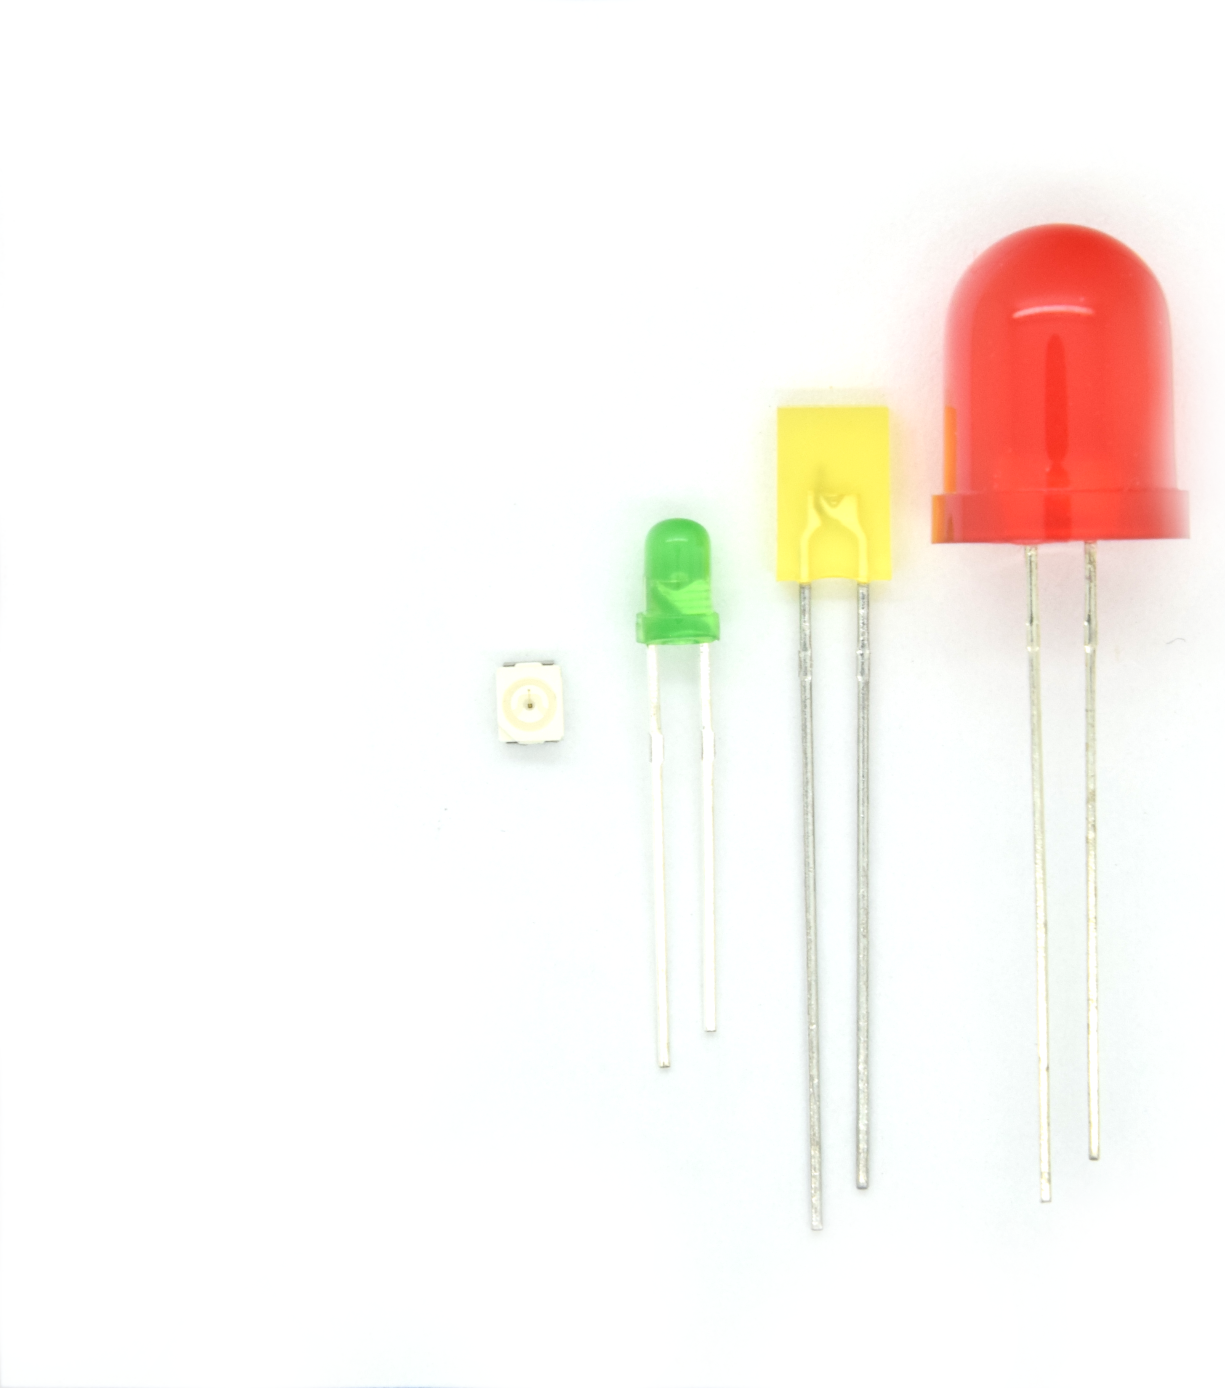
\includegraphics[width=0.85\textwidth]{foto/6}
    \caption{\scriptsize Diverse LED in verschiedenen Bauformen und Farben}
    \label{e_led}
\end{figure}

   \end{column}
\end{columns}

\end{frame}

\begin{frame}
\only<1>{
\begin{QQuestion}{EC501}{Eine in Sperrrichtung betriebene Diode zeichnet sich insbesondere aus durch~...}{eine hohe Induktivität.}
{eine hohe Kapazität.}
{eine geringe Impedanz.}
{einen hohen Widerstand.}
\end{QQuestion}

}
\only<2>{
\begin{QQuestion}{EC501}{Eine in Sperrrichtung betriebene Diode zeichnet sich insbesondere aus durch~...}{eine hohe Induktivität.}
{eine hohe Kapazität.}
{eine geringe Impedanz.}
{\textbf{\textcolor{DARCgreen}{einen hohen Widerstand.}}}
\end{QQuestion}

}
\end{frame}

\begin{frame}
\only<1>{
\begin{QQuestion}{EC502}{Wofür können Halbleiterdioden beispielsweise verwendet werden?}{zur Speicherung von Wechselströmen}
{zur Gleichrichtung von Wechselspannung}
{als Widerstand in Netzteilen}
{als Verstärker in Stromversorgungen}
\end{QQuestion}

}
\only<2>{
\begin{QQuestion}{EC502}{Wofür können Halbleiterdioden beispielsweise verwendet werden?}{zur Speicherung von Wechselströmen}
{\textbf{\textcolor{DARCgreen}{zur Gleichrichtung von Wechselspannung}}}
{als Widerstand in Netzteilen}
{als Verstärker in Stromversorgungen}
\end{QQuestion}

}
\end{frame}

\begin{frame}
\frametitle{Schwellenspannung}
\begin{columns}
    \begin{column}{0.48\textwidth}
    \begin{itemize}
  \item Damit eine Diode in Durchlassrichtung leitet, muss eine bestimmte Spannung -- die Schwellenspannung oder Durchlassspannung -- überschritten werden
  \item Je nach Basis des chemischen Elements ist die Schwellenspannung unterschiedlich hoch
  \end{itemize}

    \end{column}
   \begin{column}{0.48\textwidth}
       \begin{itemize}
  \item Germanium: \qty{0,2}{\volt}-\qty{0,4}{\volt}
  \item Silizium: \qty{0,6}{\volt}-\qty{0,8}{\volt}
  \item LED (Rot): \qty{1,6}{\volt}-\qty{2,2}{\volt}
  \item LED (Gelb, Grün): \qty{1,9}{\volt}-\qty{2,5}{\volt}
  \item LED (Blau, Weiß): \qty{2,7}{\volt}-\qty{3,5}{\volt}
  \end{itemize}

   \end{column}
\end{columns}

\end{frame}

\begin{frame}
\only<1>{
\begin{QQuestion}{EC503}{Welche typischen Schwellspannungen haben Germanium- und Siliziumdioden? Sie liegen bei~...}{Germanium zwischen \qtyrange{0,6}{0,8}{\V}, bei Silizium \qtyrange{1,4}{1,6}{\V}.}
{Germanium zwischen \qtyrange{0,6}{0,8}{\V}, bei Silizium zwischen \qtyrange{0,2}{0,4}{\V}.}
{Germanium zwischen \qtyrange{1,4}{1,6}{\V}, bei Silizium \qtyrange{0,6}{0,8}{\V}.}
{Germanium zwischen \qtyrange{0,2}{0,4}{\V}, bei Silizium zwischen \qtyrange{0,6}{0,8}{\V}.}
\end{QQuestion}

}
\only<2>{
\begin{QQuestion}{EC503}{Welche typischen Schwellspannungen haben Germanium- und Siliziumdioden? Sie liegen bei~...}{Germanium zwischen \qtyrange{0,6}{0,8}{\V}, bei Silizium \qtyrange{1,4}{1,6}{\V}.}
{Germanium zwischen \qtyrange{0,6}{0,8}{\V}, bei Silizium zwischen \qtyrange{0,2}{0,4}{\V}.}
{Germanium zwischen \qtyrange{1,4}{1,6}{\V}, bei Silizium \qtyrange{0,6}{0,8}{\V}.}
{\textbf{\textcolor{DARCgreen}{Germanium zwischen \qtyrange{0,2}{0,4}{\V}, bei Silizium zwischen \qtyrange{0,6}{0,8}{\V}.}}}
\end{QQuestion}

}
\end{frame}

\begin{frame}
\frametitle{Schottky-Diode}
\begin{itemize}
  \item Erlaubt eine hohe Schaltfrequenz
  \item Nur eine sehr niedrige Schwellenspannung von \qty{0,4}{\volt} bis unter \qty{0,1}{\volt} ist nötig
  \end{itemize}
\end{frame}

\begin{frame}
\only<1>{
\begin{QQuestion}{EC504}{Welches sind die Haupteigenschaften einer Schottkydiode?}{Sehr niedrige Durchlassspannung und sehr hohe Schaltfrequenz.}
{Sehr niedrige Durchlassspannung und sehr niedrige Schaltfrequenz.}
{Sehr hohe Durchlassspannung und sehr hohe Schaltfrequenz.}
{Sehr hohe Durchlassspannung und sehr niedrige Schaltfrequenz.}
\end{QQuestion}

}
\only<2>{
\begin{QQuestion}{EC504}{Welches sind die Haupteigenschaften einer Schottkydiode?}{\textbf{\textcolor{DARCgreen}{Sehr niedrige Durchlassspannung und sehr hohe Schaltfrequenz.}}}
{Sehr niedrige Durchlassspannung und sehr niedrige Schaltfrequenz.}
{Sehr hohe Durchlassspannung und sehr hohe Schaltfrequenz.}
{Sehr hohe Durchlassspannung und sehr niedrige Schaltfrequenz.}
\end{QQuestion}

}
\end{frame}

\begin{frame}
\frametitle{Kennlinien}
\end{frame}

\begin{frame}
\only<1>{
\begin{PQuestion}{EC506}{Welche Diode wird durch Kennlinie 2 charakterisiert?}{Germaniumdiode}
{Siliziumdiode}
{Schottkydiode}
{Leuchtdiode}
{\DARCimage{1.0\linewidth}{307include}}\end{PQuestion}

}
\only<2>{
\begin{PQuestion}{EC506}{Welche Diode wird durch Kennlinie 2 charakterisiert?}{\textbf{\textcolor{DARCgreen}{Germaniumdiode}}}
{Siliziumdiode}
{Schottkydiode}
{Leuchtdiode}
{\DARCimage{1.0\linewidth}{307include}}\end{PQuestion}

}
\end{frame}

\begin{frame}
\only<1>{
\begin{PQuestion}{EC507}{Welche Diode wird durch Kennlinie 3 charakterisiert?}{Schottkydiode}
{Leuchtdiode}
{Siliziumdiode}
{Germaniumdiode}
{\DARCimage{1.0\linewidth}{307include}}\end{PQuestion}

}
\only<2>{
\begin{PQuestion}{EC507}{Welche Diode wird durch Kennlinie 3 charakterisiert?}{Schottkydiode}
{Leuchtdiode}
{\textbf{\textcolor{DARCgreen}{Siliziumdiode}}}
{Germaniumdiode}
{\DARCimage{1.0\linewidth}{307include}}\end{PQuestion}

}
\end{frame}

\begin{frame}
\only<1>{
\begin{PQuestion}{EC508}{Welche Diode wird durch Kennlinie 4 charakterisiert?}{Leuchtdiode}
{Siliziumdiode}
{Schottkydiode}
{Germaniumdiode}
{\DARCimage{1.0\linewidth}{307include}}\end{PQuestion}

}
\only<2>{
\begin{PQuestion}{EC508}{Welche Diode wird durch Kennlinie 4 charakterisiert?}{\textbf{\textcolor{DARCgreen}{Leuchtdiode}}}
{Siliziumdiode}
{Schottkydiode}
{Germaniumdiode}
{\DARCimage{1.0\linewidth}{307include}}\end{PQuestion}

}
\end{frame}

\begin{frame}
\only<1>{
\begin{PQuestion}{EC505}{Welche Diode wird durch Kennlinie 1 charakterisiert?}{Germaniumdiode}
{Siliziumdiode}
{Schottkydiode}
{Leuchtdiode}
{\DARCimage{1.0\linewidth}{307include}}\end{PQuestion}

}
\only<2>{
\begin{PQuestion}{EC505}{Welche Diode wird durch Kennlinie 1 charakterisiert?}{Germaniumdiode}
{Siliziumdiode}
{\textbf{\textcolor{DARCgreen}{Schottkydiode}}}
{Leuchtdiode}
{\DARCimage{1.0\linewidth}{307include}}\end{PQuestion}

}
\end{frame}

\begin{frame}
\frametitle{Leitende Diode}
\begin{columns}
    \begin{column}{0.48\textwidth}
    \begin{itemize}
  \item Eine Diode leitet immer dann, wenn die Spannung an der Anode um die Schwellenspannung positiver ist als an der Kathode
  \item Gilt auch für negative Spannungen
  \item In der Prüfung kommen nur Siliziumdioden mit \qty{0,7}{\volt} Schwellenspannung vor
  \end{itemize}

    \end{column}
   \begin{column}{0.48\textwidth}
       
\begin{figure}
    \DARCimage{0.85\linewidth}{113include}
    \caption{\scriptsize Spannungen an einer leitenden Siliziumdiode}
    \label{e_leitende_siliziumdiode}
\end{figure}


   \end{column}
\end{columns}

\end{frame}

\begin{frame}
\only<1>{
\begin{QQuestion}{EC513}{Bei welcher Bedingung wird eine Siliziumdiode leitend?}{An der Anode liegen \qty{5,7}{\V}, an der Kathode \qty{5,0}{\V} an.}
{An der Anode liegen \qty{5,7}{\V}, an der Kathode \qty{6,4}{\V} an.}
{An der Anode liegen \qty{5,0}{\V}, an der Kathode \qty{5,1}{\V} an.}
{An der Anode liegen \qty{5,0}{\V}, an der Kathode \qty{5,7}{\V} an.}
\end{QQuestion}

}
\only<2>{
\begin{QQuestion}{EC513}{Bei welcher Bedingung wird eine Siliziumdiode leitend?}{\textbf{\textcolor{DARCgreen}{An der Anode liegen \qty{5,7}{\V}, an der Kathode \qty{5,0}{\V} an.}}}
{An der Anode liegen \qty{5,7}{\V}, an der Kathode \qty{6,4}{\V} an.}
{An der Anode liegen \qty{5,0}{\V}, an der Kathode \qty{5,1}{\V} an.}
{An der Anode liegen \qty{5,0}{\V}, an der Kathode \qty{5,7}{\V} an.}
\end{QQuestion}

}
\end{frame}

\begin{frame}
\only<1>{
\begin{question2x2}{EC510}{Die Auswahlantworten enthalten Siliziumdioden mit unterschiedlichen Arbeitspunkten. Bei welcher Antwort befindet sich die Diode in leitendem Zustand?}{\DARCimage{1.0\linewidth}{110include}}
{\DARCimage{1.0\linewidth}{109include}}
{\DARCimage{1.0\linewidth}{111include}}
{\DARCimage{1.0\linewidth}{112include}}
\end{question2x2}

}
\only<2>{
\begin{question2x2}{EC510}{Die Auswahlantworten enthalten Siliziumdioden mit unterschiedlichen Arbeitspunkten. Bei welcher Antwort befindet sich die Diode in leitendem Zustand?}{\DARCimage{1.0\linewidth}{110include}}
{\textbf{\textcolor{DARCgreen}{\DARCimage{1.0\linewidth}{109include}}}}
{\DARCimage{1.0\linewidth}{111include}}
{\DARCimage{1.0\linewidth}{112include}}
\end{question2x2}

}
\end{frame}

\begin{frame}
\only<1>{
\begin{question2x2}{EC509}{Die Auswahlantworten enthalten Siliziumdioden mit unterschiedlichen Arbeitspunkten. Bei welcher Antwort befindet sich die Diode in leitendem Zustand?}{\DARCimage{1.0\linewidth}{116include}}
{\DARCimage{1.0\linewidth}{114include}}
{\DARCimage{1.0\linewidth}{115include}}
{\DARCimage{1.0\linewidth}{113include}}
\end{question2x2}

}
\only<2>{
\begin{question2x2}{EC509}{Die Auswahlantworten enthalten Siliziumdioden mit unterschiedlichen Arbeitspunkten. Bei welcher Antwort befindet sich die Diode in leitendem Zustand?}{\DARCimage{1.0\linewidth}{116include}}
{\DARCimage{1.0\linewidth}{114include}}
{\DARCimage{1.0\linewidth}{115include}}
{\textbf{\textcolor{DARCgreen}{\DARCimage{1.0\linewidth}{113include}}}}
\end{question2x2}

}
\end{frame}

\begin{frame}
\only<1>{
\begin{question2x2}{EC511}{Die Auswahlantworten enthalten Siliziumdioden mit unterschiedlichen Arbeitspunkten. Bei welcher Antwort befindet sich die Diode in leitendem Zustand?}{\DARCimage{1.0\linewidth}{118include}}
{\DARCimage{1.0\linewidth}{117include}}
{\DARCimage{1.0\linewidth}{119include}}
{\DARCimage{1.0\linewidth}{120include}}
\end{question2x2}

}
\only<2>{
\begin{question2x2}{EC511}{Die Auswahlantworten enthalten Siliziumdioden mit unterschiedlichen Arbeitspunkten. Bei welcher Antwort befindet sich die Diode in leitendem Zustand?}{\DARCimage{1.0\linewidth}{118include}}
{\textbf{\textcolor{DARCgreen}{\DARCimage{1.0\linewidth}{117include}}}}
{\DARCimage{1.0\linewidth}{119include}}
{\DARCimage{1.0\linewidth}{120include}}
\end{question2x2}

}
\end{frame}

\begin{frame}
\only<1>{
\begin{question2x2}{EC512}{Die Auswahlantworten enthalten Siliziumdioden mit unterschiedlichen Arbeitspunkten. Bei welcher Antwort befindet sich die Diode in leitendem Zustand?}{\DARCimage{1.0\linewidth}{121include}}
{\DARCimage{1.0\linewidth}{122include}}
{\DARCimage{1.0\linewidth}{123include}}
{\DARCimage{1.0\linewidth}{124include}}
\end{question2x2}

}
\only<2>{
\begin{question2x2}{EC512}{Die Auswahlantworten enthalten Siliziumdioden mit unterschiedlichen Arbeitspunkten. Bei welcher Antwort befindet sich die Diode in leitendem Zustand?}{\textbf{\textcolor{DARCgreen}{\DARCimage{1.0\linewidth}{121include}}}}
{\DARCimage{1.0\linewidth}{122include}}
{\DARCimage{1.0\linewidth}{123include}}
{\DARCimage{1.0\linewidth}{124include}}
\end{question2x2}

}
\end{frame}

\begin{frame}
\frametitle{LED Anwendung }
\begin{columns}
    \begin{column}{0.48\textwidth}
    \begin{itemize}
  \item Eine LED dient als Leuchtanzeige
  \end{itemize}

    \end{column}
   \begin{column}{0.48\textwidth}
       
\begin{figure}
    \DARCimage{0.85\linewidth}{324include}
    \caption{\scriptsize LED mit Vorwiderstand}
    \label{e_led_schaltung}
\end{figure}


   \end{column}
\end{columns}

\end{frame}

\begin{frame}
\only<1>{
\begin{PQuestion}{EC514}{Wozu dient die folgende Schaltung?}{Spannungserhöhung}
{Leuchtanzeige}
{Leistungsüberwachung}
{Stromgewinnung}
{\DARCimage{0.75\linewidth}{324include}}\end{PQuestion}

}
\only<2>{
\begin{PQuestion}{EC514}{Wozu dient die folgende Schaltung?}{Spannungserhöhung}
{\textbf{\textcolor{DARCgreen}{Leuchtanzeige}}}
{Leistungsüberwachung}
{Stromgewinnung}
{\DARCimage{0.75\linewidth}{324include}}\end{PQuestion}

}
\end{frame}

\begin{frame}
\frametitle{Vorwiderstand}
\begin{columns}
    \begin{column}{0.48\textwidth}
    \begin{itemize}
  \item Da die LED selbst kaum einen Widerstand hat, würde sie bei einem direkten Anschluss an eine Spannungsquelle wie ein Kurzschluss wirken
  \item Mit einem Vorwiderstand wird der Durchlassstrom begrenzt
  \end{itemize}

    \end{column}
   \begin{column}{0.48\textwidth}
       
\begin{figure}
    \DARCimage{0.85\linewidth}{324include}
    \caption{\scriptsize LED mit Vorwiderstand}
    \label{e_led_schaltung}
\end{figure}


   \end{column}
\end{columns}

\end{frame}

\begin{frame}\begin{itemize}
  \item Berechnung: $R = \dfrac{U_q -- U_{LED}}{I_D}$
  \item $U_q$: Spannungsquelle
  \item $U_{LED}$: Schwellenspannung LED
  \item $I_D$: Durchlassstrom
  \end{itemize}
\end{frame}

\begin{frame}
\only<1>{
\begin{QQuestion}{EC515}{Eine Leuchtdiode mit einer Durchlassspannung von \qty{1,4}{\V} und einem Durchlassstrom von \qty{20}{\mA} soll an eine Spannungsquelle von \qty{5,0}{\V} angeschlossen werden. Berechnen Sie den Vorwiderstand. Die Größe des benötigten Vorwiderstandes beträgt~...}{\qty{180}{\ohm}.}
{\qty{250}{\ohm}.}
{\qty{70}{\ohm}.}
{\qty{320}{\ohm}.}
\end{QQuestion}

}
\only<2>{
\begin{QQuestion}{EC515}{Eine Leuchtdiode mit einer Durchlassspannung von \qty{1,4}{\V} und einem Durchlassstrom von \qty{20}{\mA} soll an eine Spannungsquelle von \qty{5,0}{\V} angeschlossen werden. Berechnen Sie den Vorwiderstand. Die Größe des benötigten Vorwiderstandes beträgt~...}{\textbf{\textcolor{DARCgreen}{\qty{180}{\ohm}.}}}
{\qty{250}{\ohm}.}
{\qty{70}{\ohm}.}
{\qty{320}{\ohm}.}
\end{QQuestion}

}
\end{frame}

\begin{frame}
\only<1>{
\begin{PQuestion}{EC516}{Folgende Schaltung einer Leuchtdiode wird an einer Betriebsspannung von \qty{5,5}{\V} betrieben. Der Strom durch die Leuchtdiode soll \qty{25}{\mA} betragen, wobei die Durchlassspannung \qty{1,75}{\V} beträgt. Der notwendige Vorwiderstand muss folgende Werte haben:}{\qty{150}{\ohm}/\qty{0,1}{\W}}
{\qty{150}{\ohm}/\qty{0,06}{\W}}
{\qty{70}{\ohm}/\qty{0,1}{\W}}
{\qty{70}{\ohm}/\qty{0,06}{\W}}
{\DARCimage{0.75\linewidth}{324include}}\end{PQuestion}

}
\only<2>{
\begin{PQuestion}{EC516}{Folgende Schaltung einer Leuchtdiode wird an einer Betriebsspannung von \qty{5,5}{\V} betrieben. Der Strom durch die Leuchtdiode soll \qty{25}{\mA} betragen, wobei die Durchlassspannung \qty{1,75}{\V} beträgt. Der notwendige Vorwiderstand muss folgende Werte haben:}{\textbf{\textcolor{DARCgreen}{\qty{150}{\ohm}/\qty{0,1}{\W}}}}
{\qty{150}{\ohm}/\qty{0,06}{\W}}
{\qty{70}{\ohm}/\qty{0,1}{\W}}
{\qty{70}{\ohm}/\qty{0,06}{\W}}
{\DARCimage{0.75\linewidth}{324include}}\end{PQuestion}

}
\end{frame}

\begin{frame}
\frametitle{Z-Diode}
\begin{columns}
    \begin{column}{0.48\textwidth}
    \begin{itemize}
  \item Normalerweise liegt die maximale Sperrspannung einer Diode bei ca. \qty{1000}{\volt}
  \item Bei Z-Dioden erfolgt ein Spannungsdurchbruch je nach Bauart zwischen \qty{3}{\volt} und \qty{100}{\volt}
  \item Dienen zur Spannungsstabilisierung
  \end{itemize}

    \end{column}
   \begin{column}{0.48\textwidth}
       
\begin{figure}
    \DARCimage{0.85\linewidth}{560include}
    \caption{\scriptsize Schaltzeichen Z-Diode}
    \label{_e_z_diode}
\end{figure}


   \end{column}
\end{columns}

\end{frame}

\begin{frame}
\frametitle{Polung}
\begin{columns}
    \begin{column}{0.48\textwidth}
    \begin{itemize}
  \item Z-Dioden werden mit Vorwiderstand in Sperrrichtung betrieben
  \end{itemize}

    \end{column}
   \begin{column}{0.48\textwidth}
       
\begin{figure}
    \DARCimage{0.85\linewidth}{549include}
    \caption{\scriptsize Z-Diode korrekt in Sperrichtung eingesetzt}
    \label{e_z_diode_polung}
\end{figure}


   \end{column}
\end{columns}

\end{frame}

\begin{frame}
\only<1>{
\begin{PQuestion}{EC517}{Welches Bauteil wird durch das Schaltzeichen symbolisiert?}{Z-Diode}
{Leuchtdiode}
{Kapazitätsdiode}
{Freilaufdiode}
{\DARCimage{0.5\linewidth}{560include}}\end{PQuestion}

}
\only<2>{
\begin{PQuestion}{EC517}{Welches Bauteil wird durch das Schaltzeichen symbolisiert?}{\textbf{\textcolor{DARCgreen}{Z-Diode}}}
{Leuchtdiode}
{Kapazitätsdiode}
{Freilaufdiode}
{\DARCimage{0.5\linewidth}{560include}}\end{PQuestion}

}
\end{frame}

\begin{frame}
\only<1>{
\begin{QQuestion}{EC518}{Für welchen Zweck werden Z-Dioden primär eingesetzt?}{Zur Stromstabilisierung}
{Zur Spannungsstabilisierung}
{Zur Zweiwegstabilisierung}
{Zur Leistungsstabilisierung}
\end{QQuestion}

}
\only<2>{
\begin{QQuestion}{EC518}{Für welchen Zweck werden Z-Dioden primär eingesetzt?}{Zur Stromstabilisierung}
{\textbf{\textcolor{DARCgreen}{Zur Spannungsstabilisierung}}}
{Zur Zweiwegstabilisierung}
{Zur Leistungsstabilisierung}
\end{QQuestion}

}
\end{frame}

\begin{frame}
\only<1>{
\begin{PQuestion}{EC519}{Wozu dient folgende Schaltung?}{Spannungsstabilisierung}
{Spannungserhöhung}
{Leuchtanzeige}
{Stromgewinnung}
{\DARCimage{1.0\linewidth}{549include}}\end{PQuestion}

}
\only<2>{
\begin{PQuestion}{EC519}{Wozu dient folgende Schaltung?}{\textbf{\textcolor{DARCgreen}{Spannungsstabilisierung}}}
{Spannungserhöhung}
{Leuchtanzeige}
{Stromgewinnung}
{\DARCimage{1.0\linewidth}{549include}}\end{PQuestion}

}
\end{frame}

\begin{frame}
\only<1>{
\begin{question2x2}{EC520}{In welcher der folgenden Schaltungen ist die Z-Diode zur Spannungsstabilisierung richtig eingesetzt?}{\DARCimage{1.0\linewidth}{317include}}
{\DARCimage{1.0\linewidth}{318include}}
{\DARCimage{1.0\linewidth}{319include}}
{\DARCimage{1.0\linewidth}{320include}}
\end{question2x2}

}
\only<2>{
\begin{question2x2}{EC520}{In welcher der folgenden Schaltungen ist die Z-Diode zur Spannungsstabilisierung richtig eingesetzt?}{\textbf{\textcolor{DARCgreen}{\DARCimage{1.0\linewidth}{317include}}}}
{\DARCimage{1.0\linewidth}{318include}}
{\DARCimage{1.0\linewidth}{319include}}
{\DARCimage{1.0\linewidth}{320include}}
\end{question2x2}

}
\end{frame}

\begin{frame}
\frametitle{Vorwiderstand}
\begin{columns}
    \begin{column}{0.48\textwidth}
    \begin{itemize}
  \item $U_Z$ ist die Spannung, auf die die Z-Diode stabiliert
  \item $U_V = U_1 -- U_Z = 13,8\,V -- 5\,V = 8,8\,V$
  \item $R_V = \frac{U_V}{I} = \frac{8,8\,V}{30\,mA} \approx 293\,\Omega$
  \end{itemize}

    \end{column}
   \begin{column}{0.48\textwidth}
       
\begin{figure}
    \DARCimage{0.85\linewidth}{753include}
    \caption{\scriptsize Z-Diode zur Spannungsstabilisierung}
    \label{e_z_diode_spannungsstabilisierung}
\end{figure}


   \end{column}
\end{columns}

\end{frame}

\begin{frame}
\only<1>{
\begin{PQuestion}{EC521}{Eine unbelastete Z-Diode soll eine \qty{13,8}{\V} Betriebsspannung auf \qty{5}{\V} stabilisieren. Dabei soll ein Strom von \qty{30}{\mA} durch die Z-Diode fließen. Der Ausgang der Schaltung soll nicht belastet werden. Berechnen Sie den Wert des Vorwiderstands.}{ca. \qty{167}{\ohm}}
{ca. \qty{3,41}{\milli\ohm}}
{ca. \qty{460}{\ohm}}
{ca. \qty{293}{\ohm}}
{\DARCimage{1.0\linewidth}{753include}}\end{PQuestion}

}
\only<2>{
\begin{PQuestion}{EC521}{Eine unbelastete Z-Diode soll eine \qty{13,8}{\V} Betriebsspannung auf \qty{5}{\V} stabilisieren. Dabei soll ein Strom von \qty{30}{\mA} durch die Z-Diode fließen. Der Ausgang der Schaltung soll nicht belastet werden. Berechnen Sie den Wert des Vorwiderstands.}{ca. \qty{167}{\ohm}}
{ca. \qty{3,41}{\milli\ohm}}
{ca. \qty{460}{\ohm}}
{\textbf{\textcolor{DARCgreen}{ca. \qty{293}{\ohm}}}}
{\DARCimage{1.0\linewidth}{753include}}\end{PQuestion}

}
\end{frame}

\begin{frame}
\only<1>{
\begin{PQuestion}{EC522}{Folgende Schaltung einer Stabilisierungsschaltung mit Z-Diode ist gegeben. Der Strom durch die Z-Diode soll \qty{25}{\mA} betragen und der Laststrom ist \qty{20}{\mA}. Der Wert des notwendigen Vorwiderstandes beträgt~...}{ca. \qty{364}{\ohm}.}
{ca. \qty{202}{\ohm}.}
{ca. \qty{188}{\ohm}.}
{ca. \qty{235}{\ohm}.}
{\DARCimage{1.0\linewidth}{758include}}\end{PQuestion}

}
\only<2>{
\begin{PQuestion}{EC522}{Folgende Schaltung einer Stabilisierungsschaltung mit Z-Diode ist gegeben. Der Strom durch die Z-Diode soll \qty{25}{\mA} betragen und der Laststrom ist \qty{20}{\mA}. Der Wert des notwendigen Vorwiderstandes beträgt~...}{ca. \qty{364}{\ohm}.}
{\textbf{\textcolor{DARCgreen}{ca. \qty{202}{\ohm}.}}}
{ca. \qty{188}{\ohm}.}
{ca. \qty{235}{\ohm}.}
{\DARCimage{1.0\linewidth}{758include}}\end{PQuestion}

}

\end{frame}%ENDCONTENT


\section{Transistor I}
\label{section:transistor_1}
\begin{frame}%STARTCONTENT

\frametitle{Von der Diode zum Transistor}
\begin{columns}
    \begin{column}{0.48\textwidth}
    Die Funktion kann man sich so vorstellen:

\begin{itemize}
  \item Mittels eines Steuerkanals wird der Durchfluss eines Wehrs geregelt
  \item Fließt kein Wasser im Steuerkanal ist das Wehr geschlossen
  \end{itemize}

    \end{column}
   \begin{column}{0.48\textwidth}
       
\begin{figure}
    \DARCimage{0.85\linewidth}{835include}
    \caption{\scriptsize Steuerkanal schließt Wehr komplett}
    \label{e_transistor_wehr_geschlossen}
\end{figure}


   \end{column}
\end{columns}

\end{frame}

\begin{frame}
\frametitle{Von der Diode zum Transistor}
\begin{columns}
    \begin{column}{0.48\textwidth}
    Die Funktion kann man sich so vorstellen:

\begin{itemize}
  \item Fließt etwas Wasser im Steuerkanal, öffnet das Wehr zur Hälfte
  \end{itemize}

    \end{column}
   \begin{column}{0.48\textwidth}
       
\begin{figure}
    \DARCimage{0.85\linewidth}{837include}
    \caption{\scriptsize Steuerkanal öffnet Wehr halb}
    \label{e_transistor_wehr_halb_offen}
\end{figure}


   \end{column}
\end{columns}

\end{frame}

\begin{frame}
\frametitle{Von der Diode zum Transistor}
\begin{columns}
    \begin{column}{0.48\textwidth}
    Die Funktion kann man sich so vorstellen:

\begin{itemize}
  \item Fließt mehr Wasser im Steuerkanal, ist das Wehr ganz geöffnet
  \end{itemize}

    \end{column}
   \begin{column}{0.48\textwidth}
       
\begin{figure}
    \DARCimage{0.85\linewidth}{836include}
    \caption{\scriptsize Steuerkanal öffnet Wehr komplett}
    \label{e_transistor_wehr_geoeffnet}
\end{figure}


   \end{column}
\end{columns}

\end{frame}

\begin{frame}
\only<1>{
\begin{QQuestion}{EC602}{Ein Transistor ist~...}{ein Nichtleiterbauelement.}
{ein Laserbauelement.}
{ein Halbleiterbauelement.}
{ein Kaltleiterbauelement.}
\end{QQuestion}

}
\only<2>{
\begin{QQuestion}{EC602}{Ein Transistor ist~...}{ein Nichtleiterbauelement.}
{ein Laserbauelement.}
{\textbf{\textcolor{DARCgreen}{ein Halbleiterbauelement.}}}
{ein Kaltleiterbauelement.}
\end{QQuestion}

}
\end{frame}

\begin{frame}
\only<1>{
\begin{QQuestion}{EC608}{Wie lauten die Bezeichnungen der Anschlüsse eines bipolaren Transistors?}{Emitter, Basis, Kollektor}
{Emitter, Drain, Source}
{Gate, Source, Kollektor}
{Drain, Gate, Source}
\end{QQuestion}

}
\only<2>{
\begin{QQuestion}{EC608}{Wie lauten die Bezeichnungen der Anschlüsse eines bipolaren Transistors?}{\textbf{\textcolor{DARCgreen}{Emitter, Basis, Kollektor}}}
{Emitter, Drain, Source}
{Gate, Source, Kollektor}
{Drain, Gate, Source}
\end{QQuestion}

}
\end{frame}

\begin{frame}
\frametitle{Bipolarer Transistor und Schaltbild}
\begin{columns}
    \begin{column}{0.48\textwidth}
    Merksatz für PNP $\rightarrow$ Pfeil Nach Platte


    \end{column}
   \begin{column}{0.48\textwidth}
       
\begin{figure}
    \DARCimage{0.85\linewidth}{374include}
    \caption{\scriptsize Schaltbild NPN-Transistor}
    \label{e_schaltbild_npn_transistor}
\end{figure}


\begin{figure}
    \DARCimage{0.85\linewidth}{375include}
    \caption{\scriptsize Schaltbild PNP-Transistor}
    \label{e_schaltbild_pnp_transistor}
\end{figure}


   \end{column}
\end{columns}

\end{frame}

\begin{frame}
\only<1>{
\begin{PQuestion}{EC607}{Bei diesem Bauelement handelt es sich um einen }{PNP-Transistor.}
{NPN-Transistor.}
{P-Kanal-FET.}
{N-Kanal-FET.}
{\DARCimage{0.25\linewidth}{375include}}\end{PQuestion}

}
\only<2>{
\begin{PQuestion}{EC607}{Bei diesem Bauelement handelt es sich um einen }{\textbf{\textcolor{DARCgreen}{PNP-Transistor.}}}
{NPN-Transistor.}
{P-Kanal-FET.}
{N-Kanal-FET.}
{\DARCimage{0.25\linewidth}{375include}}\end{PQuestion}

}
\end{frame}

\begin{frame}
\only<1>{
\begin{PQuestion}{EC606}{Bei diesem Bauelement handelt es sich um einen }{PNP-Transistor.}
{NPN-Transistor.}
{N-Kanal-FET.}
{P-Kanal-FET.}
{\DARCimage{0.25\linewidth}{374include}}\end{PQuestion}

}
\only<2>{
\begin{PQuestion}{EC606}{Bei diesem Bauelement handelt es sich um einen }{PNP-Transistor.}
{\textbf{\textcolor{DARCgreen}{NPN-Transistor.}}}
{N-Kanal-FET.}
{P-Kanal-FET.}
{\DARCimage{0.25\linewidth}{374include}}\end{PQuestion}

}
\end{frame}

\begin{frame}
\only<1>{
\begin{question2x2}{EC605}{Welches Schaltzeichen stellt einen bipolaren Transistor dar?}{\DARCimage{1.0\linewidth}{433include}}
{\DARCimage{1.0\linewidth}{381include}}
{\DARCimage{1.0\linewidth}{374include}}
{\DARCimage{1.0\linewidth}{432include}}
\end{question2x2}

}
\only<2>{
\begin{question2x2}{EC605}{Welches Schaltzeichen stellt einen bipolaren Transistor dar?}{\DARCimage{1.0\linewidth}{433include}}
{\DARCimage{1.0\linewidth}{381include}}
{\textbf{\textcolor{DARCgreen}{\DARCimage{1.0\linewidth}{374include}}}}
{\DARCimage{1.0\linewidth}{432include}}
\end{question2x2}

}
\end{frame}

\begin{frame}
\only<1>{
\begin{PQuestion}{EC609}{Wie bezeichnet man die Anschlüsse des abgebildeten Transistors?}{1~=~Kollektor, 2~=~Basis, 3~=~Emitter}
{1~=~Emitter, 2~=~Basis, 3~=~Kollektor}
{1~=~Kollektor, 2~=~Emitter, 3~=~Basis}
{1~=~Basis, 2~=~Emitter, 3~=~Kollektor}
{\DARCimage{0.25\linewidth}{502include}}\end{PQuestion}

}
\only<2>{
\begin{PQuestion}{EC609}{Wie bezeichnet man die Anschlüsse des abgebildeten Transistors?}{\textbf{\textcolor{DARCgreen}{1~=~Kollektor, 2~=~Basis, 3~=~Emitter}}}
{1~=~Emitter, 2~=~Basis, 3~=~Kollektor}
{1~=~Kollektor, 2~=~Emitter, 3~=~Basis}
{1~=~Basis, 2~=~Emitter, 3~=~Kollektor}
{\DARCimage{0.25\linewidth}{502include}}\end{PQuestion}

}
\end{frame}

\begin{frame}
\frametitle{Schalter oder Verstärker?}
\begin{itemize}
  \item Die Ansteuerung kann so eingestellt werden, dass der Transistor sperrt oder voll durchsteuert, dann spricht man von einem Schalttransistor.
  \item Die Ansteuerung kann so eingestellt werden, dass der Transistor stufenlos gesteuert wird, dann spricht man von einem Verstärker.
  \end{itemize}
\end{frame}

\begin{frame}
\only<1>{
\begin{QQuestion}{EC601}{Welches Bauteil kann als Schalter, Verstärker oder Widerstand eingesetzt werden?}{Diode}
{Transformator}
{Kondensator}
{Transistor}
\end{QQuestion}

}
\only<2>{
\begin{QQuestion}{EC601}{Welches Bauteil kann als Schalter, Verstärker oder Widerstand eingesetzt werden?}{Diode}
{Transformator}
{Kondensator}
{\textbf{\textcolor{DARCgreen}{Transistor}}}
\end{QQuestion}

}
\end{frame}

\begin{frame}
\only<1>{
\begin{QQuestion}{EC603}{Was versteht man unter Stromverstärkung beim Transistor?}{Mit einem geringen Kollektorstrom wird ein großer Emitterstrom gesteuert.}
{Mit einem geringen Emitterstrom wird ein großer Kollektorstrom gesteuert.}
{Mit einem geringen Emitterstrom wird ein großer Basisstrom gesteuert.}
{Mit einem geringen Basisstrom wird ein großer Kollektorstrom gesteuert.}
\end{QQuestion}

}
\only<2>{
\begin{QQuestion}{EC603}{Was versteht man unter Stromverstärkung beim Transistor?}{Mit einem geringen Kollektorstrom wird ein großer Emitterstrom gesteuert.}
{Mit einem geringen Emitterstrom wird ein großer Kollektorstrom gesteuert.}
{Mit einem geringen Emitterstrom wird ein großer Basisstrom gesteuert.}
{\textbf{\textcolor{DARCgreen}{Mit einem geringen Basisstrom wird ein großer Kollektorstrom gesteuert.}}}
\end{QQuestion}

}
\end{frame}

\begin{frame}
\frametitle{Ansteuerspannung und deren Polarität}
Je Art des bipolaren Transistor hat man verschiedene Polaritäten.

\begin{itemize}
  \item Bei einem NPN-Transistor benötigt man zum Durchschalten eine positive Steuerspannung.
  \item Bei einem PNP-Transistor benötigt man zum Durchschalten eine negative Steuerspannung.
  \end{itemize}
Die Steuerspannung liegt wie bei einer Siliziumdiode bei etwa \qty{0,6}{\volt}.

\end{frame}

\begin{frame}
\only<1>{
\begin{PQuestion}{EC610}{Wie groß muss die Spannung $U_{BE}$ in etwa sein, sodass sich der Transistor im leitenden Betriebszustand befindet?}{\qty{-0,6}{\V}}
{\qty{0,6}{\V}}
{\qty{0,6}{\V} oder \qty{-0,6}{\V}}
{\qty{0}{\V}}
{\DARCimage{0.5\linewidth}{559include}}\end{PQuestion}

}
\only<2>{
\begin{PQuestion}{EC610}{Wie groß muss die Spannung $U_{BE}$ in etwa sein, sodass sich der Transistor im leitenden Betriebszustand befindet?}{\qty{-0,6}{\V}}
{\textbf{\textcolor{DARCgreen}{\qty{0,6}{\V}}}}
{\qty{0,6}{\V} oder \qty{-0,6}{\V}}
{\qty{0}{\V}}
{\DARCimage{0.5\linewidth}{559include}}\end{PQuestion}

}
\end{frame}

\begin{frame}Da neben dem Kollektorstrom auch der Basisstrom durch den Transistor fließt, fließt durch den Emitteranschluss der größte Strom.

\end{frame}

\begin{frame}
\only<1>{
\begin{QQuestion}{EC611}{Durch welchen Transistoranschluss fliesst im leitenden Zustand der größte Strom?}{Gehäuse}
{Kollektor}
{Basis}
{Emitter}
\end{QQuestion}

}
\only<2>{
\begin{QQuestion}{EC611}{Durch welchen Transistoranschluss fliesst im leitenden Zustand der größte Strom?}{Gehäuse}
{Kollektor}
{Basis}
{\textbf{\textcolor{DARCgreen}{Emitter}}}
\end{QQuestion}

}
\end{frame}

\begin{frame}
\frametitle{ Wann schaltet der NPN Transistor durch?}
Ist die Basis-Emitter-Spannung ausreichend und liegt sie im positiven Potential vor?

Hier muss man auf die Vorzeichen achten und bei negativen Vorzeichen umdenken, Beispiele:

\begin{itemize}
  \item Basis +\qty{2}{\volt} und Emitter +\qty{1,4}{\volt}<br/> $\rightarrow$ Die Basis-Emitter-Spannung ist positiv und beträgt +\qty{0,6}{\volt}
  \item Basis -\qty{5,6}{\volt} und Emitter -\qty{6,2}{\volt}<br/> $\rightarrow$ Die Basis-Emitter-Spannung ist positiv und beträgt +\qty{0,6}{\volt}
  \end{itemize}
\end{frame}

\begin{frame}Entweder erkennet man das intuitiv oder man rechnet es (unter Beachtung der Vorzeichen) aus.

$U_{ BE } = U_{ B } -- U_{ E }$

\end{frame}

\begin{frame}
\only<1>{
\begin{question2x2}{EC612}{In einer Schaltung wurden die Spannungen der Transistoranschlüsse gegenüber Massepotential gemessen. Bei welchem der folgenden Transistoren fließt Kollektorstrom?}{\DARCimage{1.0\linewidth}{278include}}
{\DARCimage{1.0\linewidth}{279include}}
{\DARCimage{1.0\linewidth}{280include}}
{\DARCimage{1.0\linewidth}{281include}}
\end{question2x2}

}
\only<2>{
\begin{question2x2}{EC612}{In einer Schaltung wurden die Spannungen der Transistoranschlüsse gegenüber Massepotential gemessen. Bei welchem der folgenden Transistoren fließt Kollektorstrom?}{\textbf{\textcolor{DARCgreen}{\DARCimage{1.0\linewidth}{278include}}}}
{\DARCimage{1.0\linewidth}{279include}}
{\DARCimage{1.0\linewidth}{280include}}
{\DARCimage{1.0\linewidth}{281include}}
\end{question2x2}

}
\end{frame}

\begin{frame}
\only<1>{
\begin{question2x2}{EC613}{In einer Schaltung wurden die Spannungen der Transistoranschlüsse gegenüber Massepotential gemessen. Bei welchem der folgenden Transistoren fließt Kollektorstrom?}{\DARCimage{1.0\linewidth}{284include}}
{\DARCimage{1.0\linewidth}{283include}}
{\DARCimage{1.0\linewidth}{282include}}
{\DARCimage{1.0\linewidth}{285include}}
\end{question2x2}

}
\only<2>{
\begin{question2x2}{EC613}{In einer Schaltung wurden die Spannungen der Transistoranschlüsse gegenüber Massepotential gemessen. Bei welchem der folgenden Transistoren fließt Kollektorstrom?}{\DARCimage{1.0\linewidth}{284include}}
{\DARCimage{1.0\linewidth}{283include}}
{\textbf{\textcolor{DARCgreen}{\DARCimage{1.0\linewidth}{282include}}}}
{\DARCimage{1.0\linewidth}{285include}}
\end{question2x2}

}
\end{frame}

\begin{frame}
\frametitle{Wann schaltet der PNP Transistor durch?}
Ist die Basis-Emitter-Spannung ausreichend und liegt sie im negativen Potential vor?

Hier muss man auf die Vorzeichen achten und bei negativen Vorzeichen umdenken, Beispiele:

\begin{itemize}
  \item Basis +\qty{5,6}{\volt} und Emitter +\qty{6,2}{\volt}<br/> $\rightarrow$ Die Basis-Emitter-Spannung ist ist negativ und beträgt -\qty{0,6}{\volt}
  \item Basis -\qty{2}{\volt} und Emitter -\qty{1,4}{\volt}<br/> $\rightarrow$ Die Basis-Emitter-Spannung ist negativ und beträgt -\qty{0,6}{\volt}
  \end{itemize}
\end{frame}

\begin{frame}Entweder erkennet man das intuitiv oder man rechnet es (unter Beachtung der Vorzeichen) aus.

$U_{ BE } = U_{ B } -- U_{ E }$

\end{frame}

\begin{frame}
\only<1>{
\begin{question2x2}{EC614}{In einer Schaltung wurden die Spannungen der Transistoranschlüsse gegenüber Massepotential gemessen. Bei welchem der folgenden Transistoren fließt Kollektorstrom?}{\DARCimage{1.0\linewidth}{289include}}
{\DARCimage{1.0\linewidth}{287include}}
{\DARCimage{1.0\linewidth}{286include}}
{\DARCimage{1.0\linewidth}{288include}}
\end{question2x2}

}
\only<2>{
\begin{question2x2}{EC614}{In einer Schaltung wurden die Spannungen der Transistoranschlüsse gegenüber Massepotential gemessen. Bei welchem der folgenden Transistoren fließt Kollektorstrom?}{\DARCimage{1.0\linewidth}{289include}}
{\DARCimage{1.0\linewidth}{287include}}
{\textbf{\textcolor{DARCgreen}{\DARCimage{1.0\linewidth}{286include}}}}
{\DARCimage{1.0\linewidth}{288include}}
\end{question2x2}

}
\end{frame}

\begin{frame}
\only<1>{
\begin{question2x2}{EC615}{In einer Schaltung wurden die Spannungen der Transistoranschlüsse gegenüber Massepotential gemessen. Bei welchem der folgenden Transistoren fließt Kollektorstrom?}{\DARCimage{1.0\linewidth}{293include}}
{\DARCimage{1.0\linewidth}{291include}}
{\DARCimage{1.0\linewidth}{292include}}
{\DARCimage{1.0\linewidth}{290include}}
\end{question2x2}

}
\only<2>{
\begin{question2x2}{EC615}{In einer Schaltung wurden die Spannungen der Transistoranschlüsse gegenüber Massepotential gemessen. Bei welchem der folgenden Transistoren fließt Kollektorstrom?}{\DARCimage{1.0\linewidth}{293include}}
{\DARCimage{1.0\linewidth}{291include}}
{\DARCimage{1.0\linewidth}{292include}}
{\textbf{\textcolor{DARCgreen}{\DARCimage{1.0\linewidth}{290include}}}}
\end{question2x2}

}
\end{frame}

\begin{frame}
\frametitle{Typen von Transistoren}
Die bisher behandelten Transistoren nennt man \emph{Bipolare Transistoren}. Sie sind die Art der Transistoren, die in den 50er Jahren eine technische Revolution einläuteten und die Elektronenröhre ablösten. Im Gegensatz zu den stromgesteuerten Bipolartransistoren sind \emph{Feldeffekttransistoren (FET)} spannungsgesteuert, es fließt also kein Steuerstrom in ihn hinein. Mit diesen werden wir uns im Klasse~A Kurs intensiver auseinandersetzen.

\end{frame}

\begin{frame}
\only<1>{
\begin{QQuestion}{EC604}{Welche Transistortypen sind bipolare Transistoren?}{Isolierschicht-FETs}
{Dual-Gate-MOS-FETs}
{NPN- und PNP-Transistoren}
{Sperrschicht-FETs}
\end{QQuestion}

}
\only<2>{
\begin{QQuestion}{EC604}{Welche Transistortypen sind bipolare Transistoren?}{Isolierschicht-FETs}
{Dual-Gate-MOS-FETs}
{\textbf{\textcolor{DARCgreen}{NPN- und PNP-Transistoren}}}
{Sperrschicht-FETs}
\end{QQuestion}

}
\end{frame}%ENDCONTENT


\title{DARC Amateurfunklehrgang Klasse E}
\author{Reihen- und Parallelschaltung von Bauelementen}
\institute{Deutscher Amateur Radio Club e.\,V.}
\begin{frame}
\maketitle
\end{frame}

\section{Widerstand in Reihen- und Parallelschaltung}
\label{section:reihe_parallel_widerstand}
\begin{frame}%STARTCONTENT

\frametitle{Reihenschaltung}
Bei einer Reihenschaltung addieren sich die Widerstandswerte


\begin{figure}
    \DARCimage{0.85\linewidth}{812include}
    \caption{\scriptsize Reihenschaltung von 3 Widerständen}
    \label{e_reihenschaltung_von_r}
\end{figure}

$R_{ G } = R_{ 1 } + R_{ 2 } + R_{ 3 }$

Beispiel: $R_{ G } = 100 \Omega + 200 \Omega + 300 \Omega$

\end{frame}

\begin{frame}
\frametitle{Parallelschaltung}
Bei einer Parallelschaltung von Widerständen ist der Gesamtwiderstand kleiner als der Wert des kleinsten Widerstandes


\begin{figure}
    \DARCimage{0.85\linewidth}{811include}
    \caption{\scriptsize Parallelschaltung von 3 Widerständen}
    \label{e_parallelschaltung_von_r}
\end{figure}

$\frac{ 1 }{ R_{ G } } = \frac{ 1 }{ R_{ 1 } } + \frac{ 1 }{ R_{ 2 } } + \frac{ 1 }{ R_{ 3 } }$

\end{frame}

\begin{frame}Vereinfachung für zwei Widerstände:

$R_{ G } = \dfrac{ R_{ 1 } \cdot R_{ 2 } }{ R_{ 1 } + R_{ 2 }}$

\end{frame}

\begin{frame}Vereinfachung für gleiche Widerstände:

$R_{ G } = \dfrac{ R }{ n }$

$n$ steht für die Anzahl der Widerstände

\end{frame}

\begin{frame}
\only<1>{
\begin{QQuestion}{ED104}{Zwei Widerstände mit $R_1 = \qty{100}{\ohm}$ und $R_2 = \qty{400}{\ohm}$ sind parallel geschaltet. Wie groß ist der Gesamtwiderstand?}{\qty{300}{\ohm}}
{\qty{500}{\ohm}}
{\qty{80}{\ohm}}
{\qty{4}{\ohm}}
\end{QQuestion}

}
\only<2>{
\begin{QQuestion}{ED104}{Zwei Widerstände mit $R_1 = \qty{100}{\ohm}$ und $R_2 = \qty{400}{\ohm}$ sind parallel geschaltet. Wie groß ist der Gesamtwiderstand?}{\qty{300}{\ohm}}
{\qty{500}{\ohm}}
{\textbf{\textcolor{DARCgreen}{\qty{80}{\ohm}}}}
{\qty{4}{\ohm}}
\end{QQuestion}

}
\end{frame}

\begin{frame}
\only<1>{
\begin{QQuestion}{ED105}{Zwei Widerstände mit $R_1$~=~\qty{50}{\ohm} und $R_2$~=~\qty{200}{\ohm} sind parallel geschaltet. Wie groß ist der Gesamtwiderstand?}{\qty{250}{\ohm}}
{\qty{40}{\ohm}}
{\qty{150}{\ohm}}
{\qty{4}{\ohm}}
\end{QQuestion}

}
\only<2>{
\begin{QQuestion}{ED105}{Zwei Widerstände mit $R_1$~=~\qty{50}{\ohm} und $R_2$~=~\qty{200}{\ohm} sind parallel geschaltet. Wie groß ist der Gesamtwiderstand?}{\qty{250}{\ohm}}
{\textbf{\textcolor{DARCgreen}{\qty{40}{\ohm}}}}
{\qty{150}{\ohm}}
{\qty{4}{\ohm}}
\end{QQuestion}

}
\end{frame}

\begin{frame}
\only<1>{
\begin{QQuestion}{ED106}{Drei gleich große parallel geschaltete Widerstände haben einen Gesamtwiderstand von \qty{1,7}{\kohm}. Welchen Wert hat jeder Einzelwiderstand?}{\qty{2,7}{\kohm}}
{\qty{560}{\ohm}}
{\qty{10}{\kohm}}
{\qty{5,1}{\kohm}}
\end{QQuestion}

}
\only<2>{
\begin{QQuestion}{ED106}{Drei gleich große parallel geschaltete Widerstände haben einen Gesamtwiderstand von \qty{1,7}{\kohm}. Welchen Wert hat jeder Einzelwiderstand?}{\qty{2,7}{\kohm}}
{\qty{560}{\ohm}}
{\qty{10}{\kohm}}
{\textbf{\textcolor{DARCgreen}{\qty{5,1}{\kohm}}}}
\end{QQuestion}

}
\end{frame}

\begin{frame}
\frametitle{Gemischte Schaltungen}
\end{frame}

\begin{frame}
\frametitle{Variante 1: Zwei Parallel und dazu einer in Reihe}

\begin{figure}
    \DARCimage{0.85\linewidth}{813include}
    \caption{\scriptsize Gemischte Schaltung -- Variante 1}
    \label{e_gemischte_schaltung_1}
\end{figure}
    \pause
    Hier berechnet man zuerst die Parallelschaltung von $R_2$ und $R_3$ und addiert dann $R_1$ hinzu.
    \pause
    $R_{ G } = \dfrac{ R_{ 2 } \cdot R_{ 3 } }{ R_{ 2 } + R_{ 3 }} + R_{ 1 }$



\end{frame}

\begin{frame}
\frametitle{Variante 2: Zwei in Reihe und dazu einer Parallel}

\begin{figure}
    \DARCimage{0.85\linewidth}{814include}
    \caption{\scriptsize Gemischte Schaltung -- Variante 2}
    \label{e_gemischte_schaltung_2}
\end{figure}
    \pause
    Hier addiert man zuerst $R_1$ und $R_2$ um mit diesem Ergebnis die Parallelschaltung zu $R_3$ zu berechnen.
    \pause
    $R_{ G } = \dfrac{ (R_{ 1 } + R_{ 2 }) \cdot R_{ 3 }} {( R_{ 1 } + R_{ 2 }) + R_{ 3 }}$



\end{frame}

\begin{frame}
\only<1>{
\begin{PQuestion}{ED110}{Wie groß ist der Gesamtwiderstand der Schaltung? Gegeben: $R_1$ = \qty{500}{\ohm}, $R_2$ = \qty{1000}{\ohm} und $R_3$ = \qty{1}{\kohm}}{\qty{501}{\ohm}}
{\qty{2,5}{\kohm}}
{\qty{1}{\kohm}}
{\qty{5,1}{\kohm}}
{\DARCimage{1.0\linewidth}{305include}}\end{PQuestion}

}
\only<2>{
\begin{PQuestion}{ED110}{Wie groß ist der Gesamtwiderstand der Schaltung? Gegeben: $R_1$ = \qty{500}{\ohm}, $R_2$ = \qty{1000}{\ohm} und $R_3$ = \qty{1}{\kohm}}{\qty{501}{\ohm}}
{\qty{2,5}{\kohm}}
{\textbf{\textcolor{DARCgreen}{\qty{1}{\kohm}}}}
{\qty{5,1}{\kohm}}
{\DARCimage{1.0\linewidth}{305include}}\end{PQuestion}

}
\end{frame}

\begin{frame}
\only<1>{
\begin{PQuestion}{ED111}{Wie groß ist der Gesamtwiderstand der Schaltung? Gegeben: $R_1$ = \qty{1}{\kohm}, $R_2$ = \qty{2000}{\ohm} und $R_3$ = \qty{2}{\kohm}}{\qty{2}{\kohm}}
{\qty{2,5}{\kohm}}
{\qty{501}{\ohm}}
{\qty{5,1}{\kohm}}
{\DARCimage{1.0\linewidth}{305include}}\end{PQuestion}

}
\only<2>{
\begin{PQuestion}{ED111}{Wie groß ist der Gesamtwiderstand der Schaltung? Gegeben: $R_1$ = \qty{1}{\kohm}, $R_2$ = \qty{2000}{\ohm} und $R_3$ = \qty{2}{\kohm}}{\textbf{\textcolor{DARCgreen}{\qty{2}{\kohm}}}}
{\qty{2,5}{\kohm}}
{\qty{501}{\ohm}}
{\qty{5,1}{\kohm}}
{\DARCimage{1.0\linewidth}{305include}}\end{PQuestion}

}
\end{frame}

\begin{frame}
\only<1>{
\begin{PQuestion}{ED108}{Wie groß ist der Gesamtwiderstand der Schaltung? Gegeben: $R_1$~=~\qty{500}{\ohm}, $R_2$~=~\qty{500}{\ohm} und $R_3$~=~\qty{1}{\kohm}}{\qty{2}{\kohm}}
{\qty{250}{\ohm}}
{\qty{1}{\kohm}}
{\qty{500}{\ohm}}
{\DARCimage{0.5\linewidth}{378include}}\end{PQuestion}

}
\only<2>{
\begin{PQuestion}{ED108}{Wie groß ist der Gesamtwiderstand der Schaltung? Gegeben: $R_1$~=~\qty{500}{\ohm}, $R_2$~=~\qty{500}{\ohm} und $R_3$~=~\qty{1}{\kohm}}{\qty{2}{\kohm}}
{\qty{250}{\ohm}}
{\qty{1}{\kohm}}
{\textbf{\textcolor{DARCgreen}{\qty{500}{\ohm}}}}
{\DARCimage{0.5\linewidth}{378include}}\end{PQuestion}

}
\end{frame}

\begin{frame}
\only<1>{
\begin{PQuestion}{ED109}{Wie groß ist der Gesamtwiderstand der Schaltung? Gegeben: $R_1$~=~\qty{500}{\ohm}, $R_2$~=~\qty{1,5}{\kohm} und $R_3$~=~\qty{2}{\kohm}}{\qty{2}{\kohm}}
{\qty{4}{\kohm}}
{\qty{500}{\ohm}}
{\qty{1}{\kohm}}
{\DARCimage{0.5\linewidth}{378include}}\end{PQuestion}

}
\only<2>{
\begin{PQuestion}{ED109}{Wie groß ist der Gesamtwiderstand der Schaltung? Gegeben: $R_1$~=~\qty{500}{\ohm}, $R_2$~=~\qty{1,5}{\kohm} und $R_3$~=~\qty{2}{\kohm}}{\qty{2}{\kohm}}
{\qty{4}{\kohm}}
{\qty{500}{\ohm}}
{\textbf{\textcolor{DARCgreen}{\qty{1}{\kohm}}}}
{\DARCimage{0.5\linewidth}{378include}}\end{PQuestion}

}
\end{frame}

\begin{frame}
\only<1>{
\begin{PQuestion}{ED112}{Wie groß ist der Gesamtwiderstand dieser Schaltung, wenn $R_1$~=~\qty{1}{\kohm}, $R_2$~=~\qty{3}{\kohm} und $R_3$~=~\qty{1500}{\ohm} betragen?}{\qty{2}{\kohm}}
{\qty{5,5}{\kohm}}
{\qty{3,5}{\kohm}}
{\qty{1}{\kohm}}
{\DARCimage{1.0\linewidth}{305include}}\end{PQuestion}

}
\only<2>{
\begin{PQuestion}{ED112}{Wie groß ist der Gesamtwiderstand dieser Schaltung, wenn $R_1$~=~\qty{1}{\kohm}, $R_2$~=~\qty{3}{\kohm} und $R_3$~=~\qty{1500}{\ohm} betragen?}{\textbf{\textcolor{DARCgreen}{\qty{2}{\kohm}}}}
{\qty{5,5}{\kohm}}
{\qty{3,5}{\kohm}}
{\qty{1}{\kohm}}
{\DARCimage{1.0\linewidth}{305include}}\end{PQuestion}

}
\end{frame}

\begin{frame}
\only<1>{
\begin{PQuestion}{ED113}{Wie groß ist der Gesamtwiderstand dieser Schaltung, wenn $R_1$~=~\qty{10}{\kohm}, $R_2$~=~\qty{2,5}{\kohm}, $R_3$~=~\qty{500}{\ohm} und $R_4$~=~\qty{600}{\ohm} betragen? }{\qty{7,6}{\kohm}}
{\qty{13,6}{\kohm}}
{\qty{200}{\ohm}}
{\qty{1}{\kohm}}
{\DARCimage{1.0\linewidth}{385include}}\end{PQuestion}

}
\only<2>{
\begin{PQuestion}{ED113}{Wie groß ist der Gesamtwiderstand dieser Schaltung, wenn $R_1$~=~\qty{10}{\kohm}, $R_2$~=~\qty{2,5}{\kohm}, $R_3$~=~\qty{500}{\ohm} und $R_4$~=~\qty{600}{\ohm} betragen? }{\qty{7,6}{\kohm}}
{\qty{13,6}{\kohm}}
{\qty{200}{\ohm}}
{\textbf{\textcolor{DARCgreen}{\qty{1}{\kohm}}}}
{\DARCimage{1.0\linewidth}{385include}}\end{PQuestion}

}
\end{frame}

\begin{frame}
\frametitle{Belastbarkeit von Widerständen in Reihen- und Parallelschaltung}
\begin{itemize}
  \item Bei einer Reihenschaltung teilen sich die Spannungen auf.
  \item Bei einer Parallelschaltung teilen sich die Ströme auf.
  \item Somit ist bei der Berechnung mittels $P = U \cdot I$ immer ein Wert konstant und der andere entspechend kleiner.
  \item $\rightarrow$ die Gesamtbelastbarkeit ist in beiden Fällen größer als die Einzelbelastbarkeit.
  \end{itemize}
\end{frame}

\begin{frame}
\only<1>{
\begin{QQuestion}{ED107}{Welche Belastbarkeit kann die Zusammenschaltung von drei gleich großen Widerständen mit einer Einzelbelastbarkeit von je \qty{1}{\W} erreichen, wenn alle 3 Widerstände entweder parallel oder in Reihe geschaltet werden?}{\qty{1}{\W} bei Parallel- und \qty{3}{\W} bei Reihenschaltung.}
{\qty{3}{\W} bei Parallel- und \qty{1}{\W} bei Reihenschaltung.}
{\qty{3}{\W} bei Parallel- und bei Reihenschaltung.}
{\qty{1}{\W} bei Parallel- und bei Reihenschaltung.}
\end{QQuestion}

}
\only<2>{
\begin{QQuestion}{ED107}{Welche Belastbarkeit kann die Zusammenschaltung von drei gleich großen Widerständen mit einer Einzelbelastbarkeit von je \qty{1}{\W} erreichen, wenn alle 3 Widerstände entweder parallel oder in Reihe geschaltet werden?}{\qty{1}{\W} bei Parallel- und \qty{3}{\W} bei Reihenschaltung.}
{\qty{3}{\W} bei Parallel- und \qty{1}{\W} bei Reihenschaltung.}
{\textbf{\textcolor{DARCgreen}{\qty{3}{\W} bei Parallel- und bei Reihenschaltung.}}}
{\qty{1}{\W} bei Parallel- und bei Reihenschaltung.}
\end{QQuestion}

}
\end{frame}%ENDCONTENT


\section{Widerstandsnetzwerke I}
\label{section:reihe_parallel_widerstandsnetz_1}
\begin{frame}%STARTCONTENT

\begin{columns}
    \begin{column}{0.48\textwidth}
    \begin{itemize}
  \item Bei einer komplexeren Schaltung geht man wie folgt vor: In kleinere Teile auflösen und diese berechnen, danach die Schaltung neu zeichnen und überlegen wie es weitergeht
  \item Schauen wir uns die Beispielschaltung mal genauer an
  \end{itemize}

    \end{column}
   \begin{column}{0.48\textwidth}
       
\begin{figure}
    \DARCimage{0.85\linewidth}{815include}
    \caption{\scriptsize Widerstandsnetzwerk}
    \label{e_widerstandsnetzwerk_1}
\end{figure}


   \end{column}
\end{columns}

\end{frame}

\begin{frame}
\begin{columns}
    \begin{column}{0.48\textwidth}
    \begin{itemize}
  \item $R_5$ und $R_7$ liegen in Reihe und dazu ist $R_8$ parallel geschaltet. Wir berechen diese und nennen den Wert dann $R_{ 5,7,8 }$
  \item $R_3$ und $R_6$ liegen in Reihe und dazu ist $R_2$ parallel geschaltet. Wir berechen diese und nennen den Wert dann $R_{ 2,3,6 }$
  \end{itemize}

    \end{column}
   \begin{column}{0.48\textwidth}
       
\begin{figure}
    \DARCimage{0.85\linewidth}{815include}
    \caption{\scriptsize Widerstandsnetzwerk}
    \label{e_widerstandsnetzwerk_1}
\end{figure}


   \end{column}
\end{columns}

\end{frame}

\begin{frame}
\begin{columns}
    \begin{column}{0.48\textwidth}
    \begin{itemize}
  \item Dann schauen wir uns an, was von der Schaltung übrig geblieben ist.
  \item Wir sehen eine Reihenschaltung von 4 Widerständen, die sich leicht berechnen lässt.
  \item Damit können wir dann auch die folgenden Prüfungsfragen leicht beantworten.
  \end{itemize}

    \end{column}
   \begin{column}{0.48\textwidth}
       
\begin{figure}
    \DARCimage{0.85\linewidth}{817include}
    \caption{\scriptsize Widerstandsnetzwerk in der Auflösung}
    \label{e_widerstandsnetzwerk_2}
\end{figure}


   \end{column}
\end{columns}

\end{frame}

\begin{frame}
\only<1>{
\begin{PQuestion}{ED115}{Wie groß ist der Gesamtwiderstand der dargestellten Schaltung?}{\qty{383}{\ohm}}
{\qty{360}{\ohm}}
{\qty{1150}{\ohm}}
{\qty{550}{\ohm}}
{\DARCimage{1.0\linewidth}{306include}}\end{PQuestion}

}
\only<2>{
\begin{PQuestion}{ED115}{Wie groß ist der Gesamtwiderstand der dargestellten Schaltung?}{\qty{383}{\ohm}}
{\qty{360}{\ohm}}
{\qty{1150}{\ohm}}
{\textbf{\textcolor{DARCgreen}{\qty{550}{\ohm}}}}
{\DARCimage{1.0\linewidth}{306include}}\end{PQuestion}

}
\end{frame}

\begin{frame}
\only<1>{
\begin{PQuestion}{ED116}{Wie groß ist der Gesamtwiderstand der dargestellten Schaltung?}{\qty{950}{\ohm}}
{\qty{120}{\ohm}}
{\qty{2950}{\ohm}}
{\qty{750}{\ohm}}
{\DARCimage{1.0\linewidth}{395include}}\end{PQuestion}

}
\only<2>{
\begin{PQuestion}{ED116}{Wie groß ist der Gesamtwiderstand der dargestellten Schaltung?}{\textbf{\textcolor{DARCgreen}{\qty{950}{\ohm}}}}
{\qty{120}{\ohm}}
{\qty{2950}{\ohm}}
{\qty{750}{\ohm}}
{\DARCimage{1.0\linewidth}{395include}}\end{PQuestion}

}
\end{frame}%ENDCONTENT


\section{Spannungsteiler I}
\label{section:spannungsteiler_1}
\begin{frame}%STARTCONTENT

\begin{columns}
    \begin{column}{0.48\textwidth}
    \begin{itemize}
  \item Eine Reihenschaltung von Widerständen nennt man auch Spannungsteiler, weil die Spannungen sich an den Widerständen aufteilen.
  \item Je größer der Widerstand, desto größer die Spannung, die an ihm abfällt.
  \end{itemize}

    \end{column}
   \begin{column}{0.48\textwidth}
       
\begin{figure}
    \DARCimage{0.85\linewidth}{819include}
    \caption{\scriptsize Spannungsteiler}
    \label{e_spannungsteiler}
\end{figure}


   \end{column}
\end{columns}

\end{frame}

\begin{frame}
\begin{columns}
    \begin{column}{0.48\textwidth}
    \begin{itemize}
  \item Das kann man mathematisch in folgender Formel ausdrücken (Formelsammlung):
  \end{itemize}
$\dfrac{ U_{ 1 } }{ U_{ 2 } } = \dfrac{ R_{ 1 } }{ R_{ 2 } }$


    \end{column}
   \begin{column}{0.48\textwidth}
       
\begin{figure}
    \DARCimage{0.85\linewidth}{819include}
    \caption{\scriptsize Spannungsteiler}
    \label{e_spannungsteiler}
\end{figure}


   \end{column}
\end{columns}

\end{frame}

\begin{frame}Wie geht man an die Aufgaben ran?

\begin{itemize}
  \item Beispiele:
  \item Wenn $R_{ 1 }$ drei mal so groß wie $R_{ 2 }$ ist, ist $U_{ 1 }$ drei mal so groß wie $U_{ 2 }$.
  \item Wenn $R_{ 1 }$ $\frac{ 1 }{ 3 }$ so groß wie $R_{ 2 }$ ist, ist $U_{ 1 }$ $\frac{ 1 }{ 3 }$ so groß wie $U_{ 2 }$.
  \end{itemize}
Schauen wir uns dazu zwei Aufgaben an.

\end{frame}

\begin{frame}
\only<1>{
\begin{PQuestion}{ED101}{Wie teilt sich die Spannung an zwei in Reihe geschalteten Widerständen auf, wenn $R_1$~=~5-mal so groß ist wie $R_2$?}{$U_1 = 5\cdot U_2$}
{$U_1 = \frac{U_2}{5}$}
{$U_1 = 6\cdot U_2$}
{$U_1 = \frac{U_2}{6}$}
{\DARCimage{0.5\linewidth}{397include}}\end{PQuestion}

}
\only<2>{
\begin{PQuestion}{ED101}{Wie teilt sich die Spannung an zwei in Reihe geschalteten Widerständen auf, wenn $R_1$~=~5-mal so groß ist wie $R_2$?}{\textbf{\textcolor{DARCgreen}{$U_1 = 5\cdot U_2$}}}
{$U_1 = \frac{U_2}{5}$}
{$U_1 = 6\cdot U_2$}
{$U_1 = \frac{U_2}{6}$}
{\DARCimage{0.5\linewidth}{397include}}\end{PQuestion}

}
\end{frame}

\begin{frame}
\only<1>{
\begin{PQuestion}{ED102}{Wie teilt sich die Spannung an zwei in Reihe geschalteten Widerständen auf, wenn $R_1~=~\frac{1}{6}$ von $R_2$ ist? }{$U_1 = 6\cdot U_2$}
{$U_1 = \frac{U_2}{6}$}
{$U_1 = \frac{U_2}{5}$}
{$U_1 = 5\cdot U_2$}
{\DARCimage{0.5\linewidth}{397include}}\end{PQuestion}

}
\only<2>{
\begin{PQuestion}{ED102}{Wie teilt sich die Spannung an zwei in Reihe geschalteten Widerständen auf, wenn $R_1~=~\frac{1}{6}$ von $R_2$ ist? }{$U_1 = 6\cdot U_2$}
{\textbf{\textcolor{DARCgreen}{$U_1 = \frac{U_2}{6}$}}}
{$U_1 = \frac{U_2}{5}$}
{$U_1 = 5\cdot U_2$}
{\DARCimage{0.5\linewidth}{397include}}\end{PQuestion}

}
\end{frame}

\begin{frame}
\begin{columns}
    \begin{column}{0.48\textwidth}
    \begin{itemize}
  \item Die Summe der Spannnungsabfälle ist gleich der Spannung, die aus der Spannungsquelle herauskommt.
  \item Das kann man mathematisch in folgender Formel ausdrücken (Formelsammlung):
  \end{itemize}
$U_{ G } = U_{ 1 } + U_{ 2 }$


    \end{column}
   \begin{column}{0.48\textwidth}
       
\begin{figure}
    \DARCimage{0.85\linewidth}{819include}
    \caption{\scriptsize Spannungsteiler}
    \label{E 63. Spannungsteiler}
\end{figure}


   \end{column}
\end{columns}

\end{frame}

\begin{frame}
\begin{columns}
    \begin{column}{0.48\textwidth}
    \begin{itemize}
  \item Hat man eine Gesamtspannung und muss $U_{ 2 }$ berechnen, können wir ebenfalls auf eine Formel aus der Formelsammlung zurückgreifen:
  \end{itemize}
$\dfrac{ U_{ 2 } }{ U_{ G } } = \dfrac{ R_{ 2 } }{ R_{ 1 } + R_{ 2 } }$


    \end{column}
   \begin{column}{0.48\textwidth}
       
\begin{figure}
    \DARCimage{0.85\linewidth}{819include}
    \caption{\scriptsize Spannungsteiler}
    \label{E 63. Spannungsteiler}
\end{figure}


   \end{column}
\end{columns}

\end{frame}

\begin{frame}
\begin{columns}
    \begin{column}{0.48\textwidth}
    \begin{itemize}
  \item Diese muss man noch zu $U_{ 2 }$ umstellen, indem man auf beiden Seiten mit $U_{ G }$ multipliziert, dann erhält man:
  \end{itemize}
$U_{ 2 } = \dfrac{ R_{ 2 } }{ R_{ 1 } + R_{ 2 } } \cdot U_{ G }$

\begin{itemize}
  \item Damit kann man sich dann auch an die nächste Aufgabe heranwagen.
  \end{itemize}

    \end{column}
   \begin{column}{0.48\textwidth}
       
\begin{figure}
    \DARCimage{0.85\linewidth}{819include}
    \caption{\scriptsize Spannungsteiler}
    \label{E 63. Spannungsteiler}
\end{figure}


   \end{column}
\end{columns}

\end{frame}

\begin{frame}
\only<1>{
\begin{PQuestion}{ED103}{Die Gesamtspannung $U$ an folgendem Spannungsteiler beträgt \qty{9}{\V}. Die Widerstände haben die Werte $R_1$~=~\qty{10}{\kohm} und $R_2$~=~\qty{20}{\kohm}. Wie groß ist die Teilspannung $U_2$?}{\qty{4,5}{\V}}
{\qty{3,0}{\V}}
{\qty{6,0}{\V}}
{\qty{7,5}{\V}}
{\DARCimage{0.5\linewidth}{458include}}\end{PQuestion}

}
\only<2>{
\begin{PQuestion}{ED103}{Die Gesamtspannung $U$ an folgendem Spannungsteiler beträgt \qty{9}{\V}. Die Widerstände haben die Werte $R_1$~=~\qty{10}{\kohm} und $R_2$~=~\qty{20}{\kohm}. Wie groß ist die Teilspannung $U_2$?}{\qty{4,5}{\V}}
{\qty{3,0}{\V}}
{\textbf{\textcolor{DARCgreen}{\qty{6,0}{\V}}}}
{\qty{7,5}{\V}}
{\DARCimage{0.5\linewidth}{458include}}\end{PQuestion}

}
\end{frame}%ENDCONTENT


\section{Kondensator in Reihen- und Parallelschaltung}
\label{section:reihe_parallel_kondensator}
\begin{frame}%STARTCONTENT

\frametitle{Reihenschaltung}
\begin{itemize}
  \item Da die Spannung entscheidend für das Entstehen des elektrischen Feldes ist (und diese sich bei der Reihenschaltung aufteilt), ist die Berechung der Kapazität genau umgekehrt wie bei Widerständen.
  \item Anwendungsfall: Bei hohen Spannungen werden mehrere Kondensatoren in Reihe geschaltet, um die Gefahr eines Durchschlags zu verhindern. Dabei ist hilfreich, dass sich die Gesamtspannung an den Kondensatoren aufteilt.
  \end{itemize}
\end{frame}

\begin{frame}\begin{itemize}
  \item Bei einer Reihenschaltung von Kondensatoren ist die Gesamtkapazität kleiner als der Wert des kleinsten Kondensators
  \end{itemize}

\begin{figure}
    \DARCimage{0.85\linewidth}{823include}
    \caption{\scriptsize Reihenschaltung von 3 Kondensatoren}
    \label{e_reihenschaltung_kondensatoren}
\end{figure}

$\frac{ 1 }{ C_{ G } } = \frac{ 1 }{ C_{ 1 } } + \frac{ 1 }{ C_{ 2 } } + \frac{ 1 }{ C_{ 3 } }$

\end{frame}

\begin{frame}\begin{itemize}
  \item Vereinfachung für zwei Kondensatoren:
  \end{itemize}
$C_{ G } = \dfrac{ C_{ 1 } \cdot C_{ 2 } }{ C_{ 1 } + C_{ 2 }}$

\end{frame}

\begin{frame}\begin{itemize}
  \item Vereinfachung für gleiche Kondensatoren:
  \end{itemize}
$C_{ G } = \dfrac{ C }{ n }$

$n$ steht für die Anzahl der Kondensatoren

\end{frame}

\begin{frame}
\only<1>{
\begin{QQuestion}{ED119}{Eine Reihenschaltung besteht aus drei Kondensatoren von je \qty{0,33}{\micro\F}. Wie groß ist die Gesamtkapazität dieser Schaltung?}{\qty{0,110}{\micro\F}}
{\qty{0,990}{\micro\F}}
{\qty{0,011}{\micro\F}}
{\qty{0,099}{\micro\F}}
\end{QQuestion}

}
\only<2>{
\begin{QQuestion}{ED119}{Eine Reihenschaltung besteht aus drei Kondensatoren von je \qty{0,33}{\micro\F}. Wie groß ist die Gesamtkapazität dieser Schaltung?}{\textbf{\textcolor{DARCgreen}{\qty{0,110}{\micro\F}}}}
{\qty{0,990}{\micro\F}}
{\qty{0,011}{\micro\F}}
{\qty{0,099}{\micro\F}}
\end{QQuestion}

}
\end{frame}

\begin{frame}
\only<1>{
\begin{QQuestion}{ED120}{Welche Gesamtkapazität ergibt sich bei einer Reihenschaltung der Kondensatoren \qty{100}{\micro\F}, \qty{200000}{\nF} und \qty{200}{\micro\F}?}{\qty{102}{\micro\F}}
{\qty{320}{\nF}}
{\qty{300,2}{\micro\F}}
{\qty{50}{\micro\F}}
\end{QQuestion}

}
\only<2>{
\begin{QQuestion}{ED120}{Welche Gesamtkapazität ergibt sich bei einer Reihenschaltung der Kondensatoren \qty{100}{\micro\F}, \qty{200000}{\nF} und \qty{200}{\micro\F}?}{\qty{102}{\micro\F}}
{\qty{320}{\nF}}
{\qty{300,2}{\micro\F}}
{\textbf{\textcolor{DARCgreen}{\qty{50}{\micro\F}}}}
\end{QQuestion}

}
\end{frame}

\begin{frame}
\frametitle{Parallelschaltung}
\begin{itemize}
  \item Hier ist es genau umgekehrt wie bei Widerständen, weil an allen Kondensatoren die gleiche Spannung anliegt, welche ja entscheidend für die Entstehung des elektrischen Feldes ist.
  \item Anwendungsfall: Kondensatoren werden parallel geschaltet, um aus der Normreihe auf den Wert zu kommen, den man benötigt.
  \end{itemize}

\end{frame}

\begin{frame}\begin{itemize}
  \item Bei einer Parallelschaltung addieren sich die Kapazitäten
  \end{itemize}

\begin{figure}
    \DARCimage{0.85\linewidth}{822include}
    \caption{\scriptsize Parallelschaltung von 3 Kondensatoren}
    \label{e_parallelschaltung_kondensatoren}
\end{figure}

$C_{ G } = C_{ 1 } + C_{ 2 } + C_{ 3 }$

\end{frame}

\begin{frame}
\only<1>{
\begin{QQuestion}{ED117}{Drei Kondensatoren mit den Kapazitäten $C_1$ = \qty{0,1}{\micro\F}, $C_2$ = \qty{150}{\nF} und $C_3$ = \qty{50000}{\pF} werden parallel geschaltet. Wie groß ist die Gesamtkapazität?}{\qty{0,3}{\micro\F}}
{\qty{0,2}{\micro\F}}
{\qty{0,027}{\micro\F}}
{\qty{0,255}{\micro\F}}
\end{QQuestion}

}
\only<2>{
\begin{QQuestion}{ED117}{Drei Kondensatoren mit den Kapazitäten $C_1$ = \qty{0,1}{\micro\F}, $C_2$ = \qty{150}{\nF} und $C_3$ = \qty{50000}{\pF} werden parallel geschaltet. Wie groß ist die Gesamtkapazität?}{\textbf{\textcolor{DARCgreen}{\qty{0,3}{\micro\F}}}}
{\qty{0,2}{\micro\F}}
{\qty{0,027}{\micro\F}}
{\qty{0,255}{\micro\F}}
\end{QQuestion}

}
\end{frame}

\begin{frame}
\only<1>{
\begin{QQuestion}{ED118}{Wie groß ist die Gesamtkapazität von drei parallel geschalteten Kondensatoren von \qty{22}{\nF}, \qty{0,033}{\micro\F} und \qty{15000}{\pF}?}{\qty{40,3}{\nF}}
{\qty{700}{\nF}}
{\qty{0,070}{\micro\F}}
{\qty{7021}{\pF}}
\end{QQuestion}

}
\only<2>{
\begin{QQuestion}{ED118}{Wie groß ist die Gesamtkapazität von drei parallel geschalteten Kondensatoren von \qty{22}{\nF}, \qty{0,033}{\micro\F} und \qty{15000}{\pF}?}{\qty{40,3}{\nF}}
{\qty{700}{\nF}}
{\textbf{\textcolor{DARCgreen}{\qty{0,070}{\micro\F}}}}
{\qty{7021}{\pF}}
\end{QQuestion}

}
\end{frame}

\begin{frame}
\frametitle{Gemischte Schaltungen}
\end{frame}

\begin{frame}
\frametitle{Variante 1: Zwei Parallel und dazu einer in Reihe}
\begin{columns}
    \begin{column}{0.48\textwidth}
    \begin{itemize}
  \item Hier berechnet man zuerst die Parallelschaltung von $C_{ 2 }$ und $C_{ 3 }$
  \end{itemize}
$C_{ Gp } = C_{ 2 } + C_{ 3 }$

\begin{itemize}
  \item Danach berechnet man die Reihenschaltung von $C_{ 1 }$ und $C_{ Gp }$
  \end{itemize}
$C_{ G } = \frac{ C_{ 1 } \cdot C_{ Gp } }{ C_{ 1 } + C_{ Gp }}$


    \end{column}
   \begin{column}{0.48\textwidth}
       
\begin{figure}
    \DARCimage{0.85\linewidth}{820include}
    \caption{\scriptsize Gemischte Schaltung -- Variante 1}
    \label{e_gemischt_variante_1}
\end{figure}


   \end{column}
\end{columns}

\end{frame}

\begin{frame}
\only<1>{
\begin{PQuestion}{ED123}{Welche Gesamtkapazität hat die folgende Schaltung? Gegeben: $C_1$ = \qty{8}{\nF}; $C_2$ = \qty{4}{\nF}; $C_3$ = \qty{4}{\nF}}{\qty{4}{\nF}}
{\qty{16}{\nF}}
{\qty{1}{\nF}}
{\qty{9}{\nF}}
{\DARCimage{1.0\linewidth}{440include}}\end{PQuestion}

}
\only<2>{
\begin{PQuestion}{ED123}{Welche Gesamtkapazität hat die folgende Schaltung? Gegeben: $C_1$ = \qty{8}{\nF}; $C_2$ = \qty{4}{\nF}; $C_3$ = \qty{4}{\nF}}{\textbf{\textcolor{DARCgreen}{\qty{4}{\nF}}}}
{\qty{16}{\nF}}
{\qty{1}{\nF}}
{\qty{9}{\nF}}
{\DARCimage{1.0\linewidth}{440include}}\end{PQuestion}

}
\end{frame}

\begin{frame}
\only<1>{
\begin{PQuestion}{ED124}{Welche Gesamtkapazität hat diese Schaltung, wenn $C_1$ = \qty{200}{\nF}, $C_2$ = \qty{100}{\nF} und $C_3$ = \qty{100000}{\pF} betragen?}{\qty{400}{\nF}}
{\qty{250}{\nF}}
{\qty{100}{\nF}}
{\qty{200}{\nF}}
{\DARCimage{1.0\linewidth}{440include}}\end{PQuestion}

}
\only<2>{
\begin{PQuestion}{ED124}{Welche Gesamtkapazität hat diese Schaltung, wenn $C_1$ = \qty{200}{\nF}, $C_2$ = \qty{100}{\nF} und $C_3$ = \qty{100000}{\pF} betragen?}{\qty{400}{\nF}}
{\qty{250}{\nF}}
{\textbf{\textcolor{DARCgreen}{\qty{100}{\nF}}}}
{\qty{200}{\nF}}
{\DARCimage{1.0\linewidth}{440include}}\end{PQuestion}

}
\end{frame}

\begin{frame}
\only<1>{
\begin{PQuestion}{ED122}{Welche Gesamtkapazität hat diese Schaltung, wenn $C_1$~=~\qty{2}{\micro\F}, $C_2$~=~\qty{1}{\micro\F} und $C_3$~=~\qty{1}{\micro\F} betragen? }{\qty{1,0}{\micro\F}}
{\qty{4400}{\nF}}
{\qty{2,5}{\micro\F}}
{\qty{4,0}{\micro\F}}
{\DARCimage{1.0\linewidth}{440include}}\end{PQuestion}

}
\only<2>{
\begin{PQuestion}{ED122}{Welche Gesamtkapazität hat diese Schaltung, wenn $C_1$~=~\qty{2}{\micro\F}, $C_2$~=~\qty{1}{\micro\F} und $C_3$~=~\qty{1}{\micro\F} betragen? }{\textbf{\textcolor{DARCgreen}{\qty{1,0}{\micro\F}}}}
{\qty{4400}{\nF}}
{\qty{2,5}{\micro\F}}
{\qty{4,0}{\micro\F}}
{\DARCimage{1.0\linewidth}{440include}}\end{PQuestion}

}
\end{frame}

\begin{frame}
\frametitle{Variante 2: Zwei in Reihe und dazu einer Parallel}
\begin{columns}
    \begin{column}{0.48\textwidth}
    \begin{itemize}
  \item Hier berechnet man zuerst die Reihenschaltung von $C_{ 1 }$ und $C_{ 2 }$
  \end{itemize}
$C_{ Gr } = \frac{ C_{ 1 } \cdot C_{ 2 } }{ C_{ 1 } + C_{ 2 }}$

\begin{itemize}
  \item Danach berechnet man die Parallelschaltung von $C_{ 3 }$ und $C_{ Gr }$
  \end{itemize}
$C_{ G } = \frac{ C_{ 3 } \cdot C_{ Gr } }{ C_{ 3 } + C_{ Gr }}$


    \end{column}
   \begin{column}{0.48\textwidth}
       
\begin{figure}
    \DARCimage{0.85\linewidth}{457include}
    \caption{\scriptsize Gemischte Schaltung -- Variante 2}
    \label{e_gemischt_variante_2}
\end{figure}


   \end{column}
\end{columns}

\end{frame}

\begin{frame}
\only<1>{
\begin{PQuestion}{ED121}{Welche Gesamtkapazität hat die folgende Schaltung? Gegeben: $C_1$~=~\qty{10}{\nF}; $C_2$~=~\qty{10}{\nF}; $C_3$~=~\qty{5}{\nF}}{\qty{25}{\nF}}
{\qty{5}{\nF}}
{\qty{20}{\nF}}
{\qty{10}{\nF}}
{\DARCimage{1.0\linewidth}{457include}}\end{PQuestion}

}
\only<2>{
\begin{PQuestion}{ED121}{Welche Gesamtkapazität hat die folgende Schaltung? Gegeben: $C_1$~=~\qty{10}{\nF}; $C_2$~=~\qty{10}{\nF}; $C_3$~=~\qty{5}{\nF}}{\qty{25}{\nF}}
{\qty{5}{\nF}}
{\qty{20}{\nF}}
{\textbf{\textcolor{DARCgreen}{\qty{10}{\nF}}}}
{\DARCimage{1.0\linewidth}{457include}}\end{PQuestion}

}
\end{frame}%ENDCONTENT


\title{DARC Amateurfunklehrgang Klasse E}
\author{Strom- und Spannungsversorgung}
\institute{Deutscher Amateur Radio Club e.\,V.}
\begin{frame}
\maketitle
\end{frame}

\section{Spannungsquellen}
\label{section:spannungsquelle}
\begin{frame}%STARTCONTENT

\frametitle{Netzgerät}
\begin{itemize}
  \item Die für uns Funkamateuere wichtigste Spannungsquelle ist, neben Batterien, das Netzgerät. Es wird über das Stromnetz mit 230 Volt Wechselspannung versorgt und erzeut eine Gleichspannung von 13,8 Volt. Damit lassen sich Funkgeräte und Zubehör versorgen.
  \item Wichtig ist, dass die Ausggangsspannung bei Last konstant bleibt.
  \end{itemize}
\end{frame}

\begin{frame}
\only<1>{
\begin{QQuestion}{ED301}{Welche Eigenschaften sollten Gleichspannungsquellen aufweisen?}{Gleichspannungsquellen sollten bei Belastung die Spannung erhöhen.}
{Gleichspannungsquellen sollten bei Belastung eine niedrige Spannungskonstanz haben.}
{Gleichspannungsquellen sollten bei Belastung eine hohe Spannungskonstanz haben.}
{Gleichspannungsquellen sollten bei Belastung einen Wechselspannungsanteil haben.  }
\end{QQuestion}

}
\only<2>{
\begin{QQuestion}{ED301}{Welche Eigenschaften sollten Gleichspannungsquellen aufweisen?}{Gleichspannungsquellen sollten bei Belastung die Spannung erhöhen.}
{Gleichspannungsquellen sollten bei Belastung eine niedrige Spannungskonstanz haben.}
{\textbf{\textcolor{DARCgreen}{Gleichspannungsquellen sollten bei Belastung eine hohe Spannungskonstanz haben.}}}
{Gleichspannungsquellen sollten bei Belastung einen Wechselspannungsanteil haben.  }
\end{QQuestion}

}
\end{frame}

\begin{frame}
\frametitle{Elektrische Sicherheit}
Bei Netzgeräten, besonders mit einem Metallgehäuse, ist ein normgerechter Anschluss an das Stromnetz wichtig. Der Schutzleiter (grün/gelb) hat dabei die Aufgabe im Fehlerfall die Spannung zur \enquote{Erde} abzuleiten und damit die Haussicherung auszulösen, damit keine gefährliche Spannung am Metallgehäuse anliegt. Bei einer 3-adrigen Leitung sind die Adernkennfarben wie folgt festgelegt:

\end{frame}

\begin{frame}
\frametitle{Aderfarben}
\begin{columns}
    \begin{column}{0.48\textwidth}
    \begin{itemize}
  \item Außenleiter (L) $\rightarrow$ braun
  \item Neutralleiter (N) $\rightarrow$ blau
  \item Schutzleiter (PE) $\rightarrow$ grün/gelb
  \end{itemize}

    \end{column}
   \begin{column}{0.48\textwidth}
       
\begin{figure}
    \DARCimage{0.85\linewidth}{791include}
    \caption{\scriptsize Aderfarben einer 3-adrigen Leitung}
    \label{e_NYM_Aderfarben}
\end{figure}


   \end{column}
\end{columns}

\end{frame}

\begin{frame}
\only<1>{
\begin{QQuestion}{EK205}{Wählen Sie die normgerechten Adernkennfarben von 3-adrigen, isolierten Energieleitungen und -kabeln in der Reihenfolge: Schutzleiter, Außenleiter, Neutralleiter!}{grüngelb, braun, blau}
{braun, grüngelb, blau}
{grau, schwarz, rot}
{grüngelb, blau, braun oder schwarz}
\end{QQuestion}

}
\only<2>{
\begin{QQuestion}{EK205}{Wählen Sie die normgerechten Adernkennfarben von 3-adrigen, isolierten Energieleitungen und -kabeln in der Reihenfolge: Schutzleiter, Außenleiter, Neutralleiter!}{\textbf{\textcolor{DARCgreen}{grüngelb, braun, blau}}}
{braun, grüngelb, blau}
{grau, schwarz, rot}
{grüngelb, blau, braun oder schwarz}
\end{QQuestion}

}
\end{frame}%ENDCONTENT


\section{Gleichrichter I}
\label{section:gleichrichter_1}
\begin{frame}%STARTCONTENT

\frametitle{Gleichrichter}
\begin{columns}
    \begin{column}{0.48\textwidth}
    \begin{itemize}
  \item Um die Wechselspannung zu einer Gleichspannung zu wandeln, benötigen wir einen Gleichrichter.
  \item Die einfachste Möglichkeit ist die Gleichrichtung mit einer Diode, denn eine Diode leitet den Strom nur in eine Richtung.
  \end{itemize}

    \end{column}
   \begin{column}{0.48\textwidth}
       
\begin{figure}
    \DARCimage{0.85\linewidth}{797include}
    \caption{\scriptsize Einweggleichrichter}
    \label{e_einweggleichrichter}
\end{figure}


   \end{column}
\end{columns}

\end{frame}

\begin{frame}
\begin{columns}
    \begin{column}{0.48\textwidth}
    \begin{itemize}
  \item Damit \enquote{schneiden} wir von der Wechselspannung die negative Halbwelle ab.
  \item Weitere Bauelemente sind notwendig um aus den positiven Halbwellen eine stabile Gleichspannung zu machen, diese lernen wir im Klasse~A Kurs kennen.
  \end{itemize}

    \end{column}
   \begin{column}{0.48\textwidth}
       
\begin{figure}
    \DARCimage{0.85\linewidth}{798include}
    \caption{\scriptsize Eingangsspannung Einweggleichrichter}
    \label{e_einweggleichrichter_ue}
\end{figure}


\begin{figure}
    \DARCimage{0.85\linewidth}{796include}
    \caption{\scriptsize Lastspannung Einweggleichrichter}
    \label{e_einweggleichrichter_ul}
\end{figure}


   \end{column}
\end{columns}

\end{frame}

\begin{frame}
\only<1>{
\begin{PQuestion}{ED304}{Welchen Verlauf hat die Spannung $U$?}{\DARCimage{1.0\linewidth}{215include}}
{\DARCimage{1.0\linewidth}{214include}}
{\DARCimage{1.0\linewidth}{216include}}
{\DARCimage{1.0\linewidth}{217include}}
{\DARCimage{1.0\linewidth}{304include}}\end{PQuestion}

}
\only<2>{
\begin{PQuestion}{ED304}{Welchen Verlauf hat die Spannung $U$?}{\DARCimage{1.0\linewidth}{215include}}
{\textbf{\textcolor{DARCgreen}{\DARCimage{1.0\linewidth}{214include}}}}
{\DARCimage{1.0\linewidth}{216include}}
{\DARCimage{1.0\linewidth}{217include}}
{\DARCimage{1.0\linewidth}{304include}}\end{PQuestion}

}
\end{frame}%ENDCONTENT


\section{Schaltnetzteil I}
\label{section:schaltnetzteil_1}
\begin{frame}%STARTCONTENT
\begin{itemize}
  \item Das im vorigen Kapitel vorgestellte Netzteil hat den Nachteil eines hohen Gewichts durch den Transformator und einen schlechten Wirkungsgrad aufgrund von Verlusten bei der Konstanthaltung der Ausgangsspannung.
  \item Schaltnetzteile bringen die Eingangsspannung auf eine höhere Frequenz, wodurch kleinere Transformatoren eingesetzt werden können und bieten effizientere Wege die Ausgangsspannung konstant zu halten.
  \end{itemize}
\end{frame}

\begin{frame}Details auch hier im Klasse~A Kurs, wir konzentrieren uns auf die positiven Eigenschaften:

\begin{itemize}
  \item \emph{Hoher Wirkungsgrad}
  \item \emph{Geringes Gewicht}
  \item \emph{Geringes Volumen}
  \end{itemize}
\end{frame}

\begin{frame}
\only<1>{
\begin{QQuestion}{ED302}{Welche Eigenschaften hat ein Schaltnetzteil?}{Hoher Wirkungsgrad, geringes Gewicht, geringes Volumen.}
{Niedriger Wirkungsgrad, geringes Gewicht, geringes Volumen.}
{Hoher Wirkungsgrad, hohes Gewicht, geringes Volumen.}
{Hoher Wirkungsgrad, geringes Gewicht, großes Volumen.}
\end{QQuestion}

}
\only<2>{
\begin{QQuestion}{ED302}{Welche Eigenschaften hat ein Schaltnetzteil?}{\textbf{\textcolor{DARCgreen}{Hoher Wirkungsgrad, geringes Gewicht, geringes Volumen.}}}
{Niedriger Wirkungsgrad, geringes Gewicht, geringes Volumen.}
{Hoher Wirkungsgrad, hohes Gewicht, geringes Volumen.}
{Hoher Wirkungsgrad, geringes Gewicht, großes Volumen.}
\end{QQuestion}

}
\end{frame}

\begin{frame}Aber: Wo Licht ist, ist auch Schatten.

\begin{itemize}
  \item Durch die hohen Frequenzen kann es zu \emph{hochfrequenten Störungen} kommen, die besonders im Kurzwellenbereich stören.
  \item Bei für den Amateurfunk konzipierten Netzgeräten ist das inzwischen kein Problem mehr, bei Netzgeräten in der Unterhaltungselektronik schon.
  \end{itemize}
\end{frame}

\begin{frame}
\only<1>{
\begin{QQuestion}{ED303}{Welches ist der Hauptnachteil eines Schaltnetzteils ?}{Ein Schaltnetzteil kann keine so hohen Ströme abgeben.}
{Ein Schaltnetzteil hat einen niedrigen Wirkungsgrad.}
{Ein Schaltnetzteil kann hochfrequente Störungen erzeugen.}
{Ein Schaltnetzteil hat hohe Verluste.}
\end{QQuestion}

}
\only<2>{
\begin{QQuestion}{ED303}{Welches ist der Hauptnachteil eines Schaltnetzteils ?}{Ein Schaltnetzteil kann keine so hohen Ströme abgeben.}
{Ein Schaltnetzteil hat einen niedrigen Wirkungsgrad.}
{\textbf{\textcolor{DARCgreen}{Ein Schaltnetzteil kann hochfrequente Störungen erzeugen.}}}
{Ein Schaltnetzteil hat hohe Verluste.}
\end{QQuestion}

}
\end{frame}%ENDCONTENT


\section{Sicherungen}
\label{section:sicherungen}
\begin{frame}%STARTCONTENT

\begin{columns}
    \begin{column}{0.48\textwidth}
    \begin{itemize}
  \item Im Netzgerät und/oder in der Verbindungsleitung zum Transceiver gibt es sogenannte Feinsicherungen
  \item Diese unterbrechen im Fehlerfall (Kurzschluss oder Überlastung) den Stromfluss
  \end{itemize}

    \end{column}
   \begin{column}{0.48\textwidth}
       
\begin{figure}
    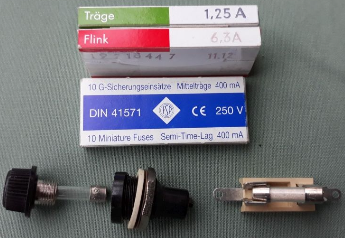
\includegraphics[width=0.85\textwidth]{foto/88}
    \caption{\scriptsize Feinsicherungen}
    \label{n_feinsicherungen}
\end{figure}

   \end{column}
\end{columns}

\end{frame}

\begin{frame}\begin{itemize}
  \item Nachdem eine Feinsicherung ausgelöst hat und man die Ursache behoben hat, muss man sie austauschen.
  \item Defekte Sicherungen dürfen \emph{nur durch gleichartige ersetzt werden}!
  \item Dabei ist sowohl auf \emph{Stromstärke} als auch die \emph{Auslösecharakteristik} zu achten, die angibt, wie schnell eine Sicherung auslöst (flink, mittelträge, träge).
  \end{itemize}
\end{frame}

\begin{frame}\begin{table}
\begin{DARCtabular}{ccc}
     Auslösecharakteristik  & Kennzeichen  & Abschaltzeit bei zehnfachem Nennstrom   \\
     flink  & F  & max. 30 ms  \\
     mittelträge  & MT  & max. 90 ms   \\
     träge  & T  & max. 300 ms   \\
\end{DARCtabular}
\caption{Kenngrößen von Feinsicherungen}
\label{n_feinsicherung}
\end{table}
\end{frame}

\begin{frame}
\only<1>{
\begin{QQuestion}{EK204}{Sie haben in ihren Kurzwellensender soeben einen Kurzschluss im Netzteil erfolgreich repariert. Durch den Fehler wurde auch die Feinsicherung für die Stromversorgung mit der Aufschrift \qty{20}{\A} \glqq Flink\grqq{} zerstört. Beim Austausch dieser Sicherung~...}{darf der Stromwert auch größer als \qty{20}{\A} sein, es muß jedoch eine Sicherung mit Auslösecharakteristik \glqq Flink\grqq{} eingesetzt werden.}
{darf bei gleichem Stromwert auch eine Sicherung mit Auslösecharakteristik \glqq Mittelträge\grqq{} oder \glqq Träge\grqq{} eingesetzt werden.}
{sollte eine Sicherung gleichen Stromwertes und gleicher Auslösecharakteristik eingesetzt werden.}
{kann ersatzweise auch eine Drahtbrücke aus dünnem Kupferdraht eingesetzt werden.}
\end{QQuestion}

}
\only<2>{
\begin{QQuestion}{EK204}{Sie haben in ihren Kurzwellensender soeben einen Kurzschluss im Netzteil erfolgreich repariert. Durch den Fehler wurde auch die Feinsicherung für die Stromversorgung mit der Aufschrift \qty{20}{\A} \glqq Flink\grqq{} zerstört. Beim Austausch dieser Sicherung~...}{darf der Stromwert auch größer als \qty{20}{\A} sein, es muß jedoch eine Sicherung mit Auslösecharakteristik \glqq Flink\grqq{} eingesetzt werden.}
{darf bei gleichem Stromwert auch eine Sicherung mit Auslösecharakteristik \glqq Mittelträge\grqq{} oder \glqq Träge\grqq{} eingesetzt werden.}
{\textbf{\textcolor{DARCgreen}{sollte eine Sicherung gleichen Stromwertes und gleicher Auslösecharakteristik eingesetzt werden.}}}
{kann ersatzweise auch eine Drahtbrücke aus dünnem Kupferdraht eingesetzt werden.}
\end{QQuestion}

}
\end{frame}%ENDCONTENT


\title{DARC Amateurfunklehrgang Klasse E}
\author{Grundlegende Schaltungen}
\institute{Deutscher Amateur Radio Club e.\,V.}
\begin{frame}
\maketitle
\end{frame}

\section{Schwingkreis I}
\label{section:schwingkreis_1}
\begin{frame}%STARTCONTENT
\begin{itemize}
  \item Kondensatoren und Spulen haben frequenzabhängige Widerstände
  \item Damit sind passive Filterschaltungen möglich, um nur bestimmte Frequenzen passieren zu lassen
  \end{itemize}
    \pause
    \emph{Zur Erinnerung}

\begin{itemize}
  \item Kondensator blockiert niedrige Frequenzen und  lässt hohe Frequenzen durch
  \item Spule blockiert hohe Frequenzen und lässt niedrige Frequenzen durch
  \end{itemize}


\end{frame}

\begin{frame}
\frametitle{Hochpass}
\begin{columns}
    \begin{column}{0.48\textwidth}
    \begin{itemize}
  \item Bei niedrigen Frequenzen hat der Kondensator einen sehr hohen Widerstand
  \item Schaltung wirkt wie ein frequenzabhängiger Spannungsteiler
  \item U<sub>A</sub> ist dadurch sehr klein
  \end{itemize}

    \end{column}
   \begin{column}{0.48\textwidth}
       
\begin{figure}
    \DARCimage{0.85\linewidth}{592include}
    \caption{\scriptsize Filtercharakteristik eines Hochpass}
    \label{e_hochpass}
\end{figure}


\begin{figure}
    \DARCimage{0.85\linewidth}{195include}
    \caption{\scriptsize Hochpass aus Kondensator und Widerstand}
    \label{e_hochpass_rc}
\end{figure}


   \end{column}
\end{columns}

\end{frame}

\begin{frame}
\only<1>{
\begin{PQuestion}{ED202}{Wie wird die dargestellte Filtercharakteristik bezeichnet?}{Bandsperre}
{Tiefpass}
{Bandpass}
{Hochpass}
{\DARCimage{0.75\linewidth}{592include}}\end{PQuestion}

}
\only<2>{
\begin{PQuestion}{ED202}{Wie wird die dargestellte Filtercharakteristik bezeichnet?}{Bandsperre}
{Tiefpass}
{Bandpass}
{\textbf{\textcolor{DARCgreen}{Hochpass}}}
{\DARCimage{0.75\linewidth}{592include}}\end{PQuestion}

}
\end{frame}

\begin{frame}
\only<1>{
\begin{PQuestion}{ED211}{Was stellt die folgende Schaltung dar? }{Hochpass}
{Sperrkreis}
{Bandpass}
{Tiefpass}
{\DARCimage{1.0\linewidth}{195include}}\end{PQuestion}

}
\only<2>{
\begin{PQuestion}{ED211}{Was stellt die folgende Schaltung dar? }{\textbf{\textcolor{DARCgreen}{Hochpass}}}
{Sperrkreis}
{Bandpass}
{Tiefpass}
{\DARCimage{1.0\linewidth}{195include}}\end{PQuestion}

}
\end{frame}

\begin{frame}
\only<1>{
\begin{PQuestion}{ED212}{Was stellt die folgende Schaltung dar? }{Hochpass}
{Sperrkreis}
{Bandpass}
{Tiefpass}
{\DARCimage{1.0\linewidth}{754include}}\end{PQuestion}

}
\only<2>{
\begin{PQuestion}{ED212}{Was stellt die folgende Schaltung dar? }{\textbf{\textcolor{DARCgreen}{Hochpass}}}
{Sperrkreis}
{Bandpass}
{Tiefpass}
{\DARCimage{1.0\linewidth}{754include}}\end{PQuestion}

}

\end{frame}

\begin{frame}
\only<1>{
\begin{question2x2}{ED213}{Welche Schaltung stellt ein Hochpassfilter dar?}{\DARCimage{1.0\linewidth}{182include}}
{\DARCimage{1.0\linewidth}{167include}}
{\DARCimage{1.0\linewidth}{172include}}
{\DARCimage{1.0\linewidth}{165include}}
\end{question2x2}

}
\only<2>{
\begin{question2x2}{ED213}{Welche Schaltung stellt ein Hochpassfilter dar?}{\DARCimage{1.0\linewidth}{182include}}
{\DARCimage{1.0\linewidth}{167include}}
{\DARCimage{1.0\linewidth}{172include}}
{\textbf{\textcolor{DARCgreen}{\DARCimage{1.0\linewidth}{165include}}}}
\end{question2x2}

}

\end{frame}

\begin{frame}
\frametitle{Tiefpass}
\begin{columns}
    \begin{column}{0.48\textwidth}
    \begin{itemize}
  \item Bei niedrigen Frequenzen hat der Kondensator einen sehr hohen Widerstand
  \item Schaltung wirkt wie ein frequenzabhängiger Spannungsteiler
  \item U<sub>A</sub> ist dadurch sehr groß
  \end{itemize}

    \end{column}
   \begin{column}{0.48\textwidth}
       
\begin{figure}
    \DARCimage{0.85\linewidth}{591include}
    \caption{\scriptsize Filtercharakteristik eines Tiefpass}
    \label{e_hochpass}
\end{figure}


\begin{figure}
    \DARCimage{0.85\linewidth}{175include}
    \caption{\scriptsize Tiefpass aus Kondensator und Widerstand}
    \label{e_tiefpass_rc}
\end{figure}


   \end{column}
\end{columns}

\end{frame}

\begin{frame}
\only<1>{
\begin{PQuestion}{ED201}{Wie wird die dargestellte Filtercharakteristik bezeichnet?}{Bandsperre}
{Hochpass}
{Bandpass}
{Tiefpass}
{\DARCimage{0.75\linewidth}{591include}}\end{PQuestion}

}
\only<2>{
\begin{PQuestion}{ED201}{Wie wird die dargestellte Filtercharakteristik bezeichnet?}{Bandsperre}
{Hochpass}
{Bandpass}
{\textbf{\textcolor{DARCgreen}{Tiefpass}}}
{\DARCimage{0.75\linewidth}{591include}}\end{PQuestion}

}
\end{frame}

\begin{frame}
\only<1>{
\begin{PQuestion}{ED208}{Was stellt die folgende Schaltung dar? }{Bandpass}
{Sperrkreis}
{Tiefpass}
{Hochpass}
{\DARCimage{1.0\linewidth}{175include}}\end{PQuestion}

}
\only<2>{
\begin{PQuestion}{ED208}{Was stellt die folgende Schaltung dar? }{Bandpass}
{Sperrkreis}
{\textbf{\textcolor{DARCgreen}{Tiefpass}}}
{Hochpass}
{\DARCimage{1.0\linewidth}{175include}}\end{PQuestion}

}
\end{frame}

\begin{frame}
\only<1>{
\begin{PQuestion}{ED209}{Was stellt die folgende Schaltung dar? }{Tiefpass}
{Sperrkreis}
{Bandpass}
{Hochpass}
{\DARCimage{1.0\linewidth}{756include}}\end{PQuestion}

}
\only<2>{
\begin{PQuestion}{ED209}{Was stellt die folgende Schaltung dar? }{\textbf{\textcolor{DARCgreen}{Tiefpass}}}
{Sperrkreis}
{Bandpass}
{Hochpass}
{\DARCimage{1.0\linewidth}{756include}}\end{PQuestion}

}

\end{frame}

\begin{frame}
\only<1>{
\begin{question2x2}{ED210}{Welche Schaltung könnte für die Tiefpassfilterung in einem Mikrofonverstärker eingesetzt werden?}{\DARCimage{1.0\linewidth}{170include}}
{\DARCimage{1.0\linewidth}{173include}}
{\DARCimage{1.0\linewidth}{161include}}
{\DARCimage{1.0\linewidth}{169include}}
\end{question2x2}

}
\only<2>{
\begin{question2x2}{ED210}{Welche Schaltung könnte für die Tiefpassfilterung in einem Mikrofonverstärker eingesetzt werden?}{\textbf{\textcolor{DARCgreen}{\DARCimage{1.0\linewidth}{170include}}}}
{\DARCimage{1.0\linewidth}{173include}}
{\DARCimage{1.0\linewidth}{161include}}
{\DARCimage{1.0\linewidth}{169include}}
\end{question2x2}

}

\end{frame}

\begin{frame}
\frametitle{Serienschwingkreis}
\begin{columns}
    \begin{column}{0.48\textwidth}
    \begin{itemize}
  \item Es gibt eine Resonanzfrequenz, bei der der Wechselstromwiderstand (Impedanz) sehr gering ist
  \item Bandpass, Saugkreis (eine Frequenz wird rausgesaugt)
  \end{itemize}

    \end{column}
   \begin{column}{0.48\textwidth}
       
\begin{figure}
    \DARCimage{0.85\linewidth}{189include}
    \caption{\scriptsize Impedanzverlauf eines Serienschwingkreis}
    \label{e_serienschwingkreis_z}
\end{figure}


\begin{figure}
    \DARCimage{0.85\linewidth}{757include}
    \caption{\scriptsize Serienschwingkreis aus Kondensator und Spule}
    \label{e_serienschwingkreis_cl}
\end{figure}


   \end{column}
\end{columns}

\end{frame}%ENDCONTENT


\section{Oszillatoren}
\label{section:oszillatoren}
\begin{frame}%STARTCONTENT
\begin{itemize}
  \item Oszillatoren erzeugen eine Wechselspannung
  \item Es gibt verschiedene Methoden
  \end{itemize}
\end{frame}

\begin{frame}
\frametitle{LC-Oszillator}
\begin{columns}
    \begin{column}{0.48\textwidth}
    \begin{itemize}
  \item Schwingungserzeugung mit Spule und Kondensator als Schwingkreis
  \item Ein aufgeladener Kondensator entlädt sich an der Spule
  \item Eine aufgeladene Spule entlädt sich am Kondensator
  \item Je nach Wert der Bauteile in einer bestimmten Frequenz
  \end{itemize}

    \end{column}
   \begin{column}{0.48\textwidth}
       
\begin{figure}
    \DARCimage{0.85\linewidth}{755include}
    \caption{\scriptsize Parallelschwingkreis aus Kondensator und Spule}
    \label{e_parallelschwingkreis_cl}
\end{figure}


   \end{column}
\end{columns}

\end{frame}

\begin{frame}
\only<1>{
\begin{QQuestion}{ED501}{Was ist ein LC-Oszillator? Es ist ein Schwingungserzeuger, wobei die Frequenz~...}{mittels LC-Tiefpass gefiltert wird.}
{durch einen hochstabilen Quarz bestimmt wird.}
{von einer Spule und einem Kondensator als Schwingkreis bestimmt wird.}
{mittels LC-Hochpass gefiltert wird.}
\end{QQuestion}

}
\only<2>{
\begin{QQuestion}{ED501}{Was ist ein LC-Oszillator? Es ist ein Schwingungserzeuger, wobei die Frequenz~...}{mittels LC-Tiefpass gefiltert wird.}
{durch einen hochstabilen Quarz bestimmt wird.}
{\textbf{\textcolor{DARCgreen}{von einer Spule und einem Kondensator als Schwingkreis bestimmt wird.}}}
{mittels LC-Hochpass gefiltert wird.}
\end{QQuestion}

}
\end{frame}

\begin{frame}
\frametitle{Temperaturstabilität}
\begin{columns}
    \begin{column}{0.48\textwidth}
    \begin{itemize}
  \item Die passiven Bauelemente haben bei veränderlicher Temperatur unterschiedliche Werte
  \end{itemize}

    \end{column}
   \begin{column}{0.48\textwidth}
       \begin{itemize}
  \item Höhere Frequenz bei \emph{kleinerer} Kapazität oder Induktivität
  \item Niedrigere Frequenz bei \emph{höherer} Kapazität oder Induktivität
  \end{itemize}

   \end{column}
\end{columns}

\end{frame}

\begin{frame}
\only<1>{
\begin{QQuestion}{ED502}{Wie verhält sich die Frequenz eines LC-Oszillators, wenn bei zunehmender Temperatur die Kapazität des Kondensators größer wird?}{Die Frequenz wird höher.}
{Die Schwingungen reißen sofort ab.}
{Die Frequenz wird niedriger.}
{Die Frequenz bleibt stabil.}
\end{QQuestion}

}
\only<2>{
\begin{QQuestion}{ED502}{Wie verhält sich die Frequenz eines LC-Oszillators, wenn bei zunehmender Temperatur die Kapazität des Kondensators größer wird?}{Die Frequenz wird höher.}
{Die Schwingungen reißen sofort ab.}
{\textbf{\textcolor{DARCgreen}{Die Frequenz wird niedriger.}}}
{Die Frequenz bleibt stabil.}
\end{QQuestion}

}
\end{frame}

\begin{frame}
\only<1>{
\begin{QQuestion}{ED503}{Wie verhält sich die Frequenz eines LC-Oszillators, wenn bei zunehmender Temperatur die Kapazität des Kondensators kleiner wird?}{Die Frequenz wird höher.}
{Die Schwingungen reißen sofort ab.}
{Die Frequenz wird niedriger.}
{Die Frequenz bleibt stabil.}
\end{QQuestion}

}
\only<2>{
\begin{QQuestion}{ED503}{Wie verhält sich die Frequenz eines LC-Oszillators, wenn bei zunehmender Temperatur die Kapazität des Kondensators kleiner wird?}{\textbf{\textcolor{DARCgreen}{Die Frequenz wird höher.}}}
{Die Schwingungen reißen sofort ab.}
{Die Frequenz wird niedriger.}
{Die Frequenz bleibt stabil.}
\end{QQuestion}

}
\end{frame}

\begin{frame}
\only<1>{
\begin{QQuestion}{ED504}{Wie verhält sich die Frequenz eines LC-Oszillators, wenn bei zunehmender Temperatur die Induktivität der Spule größer wird?}{Die Frequenz bleibt stabil.}
{Die Frequenz wird höher.}
{Die Frequenz wird niedriger.}
{Die Schwingungen reißen sofort ab.}
\end{QQuestion}

}
\only<2>{
\begin{QQuestion}{ED504}{Wie verhält sich die Frequenz eines LC-Oszillators, wenn bei zunehmender Temperatur die Induktivität der Spule größer wird?}{Die Frequenz bleibt stabil.}
{Die Frequenz wird höher.}
{\textbf{\textcolor{DARCgreen}{Die Frequenz wird niedriger.}}}
{Die Schwingungen reißen sofort ab.}
\end{QQuestion}

}
\end{frame}

\begin{frame}
\only<1>{
\begin{QQuestion}{ED505}{Wie verhält sich die Frequenz eines LC-Oszillators, wenn bei zunehmender Temperatur die Induktivität der Spule kleiner wird?}{Die Schwingungen reißen sofort ab.}
{Die Frequenz wird niedriger.}
{Die Frequenz wird höher.}
{Die Frequenz bleibt stabil.}
\end{QQuestion}

}
\only<2>{
\begin{QQuestion}{ED505}{Wie verhält sich die Frequenz eines LC-Oszillators, wenn bei zunehmender Temperatur die Induktivität der Spule kleiner wird?}{Die Schwingungen reißen sofort ab.}
{Die Frequenz wird niedriger.}
{\textbf{\textcolor{DARCgreen}{Die Frequenz wird höher.}}}
{Die Frequenz bleibt stabil.}
\end{QQuestion}

}
\end{frame}

\begin{frame}
\only<1>{
\begin{QQuestion}{EF304}{Der VFO eines Senders ist schwankenden Temperaturen unterworfen. Welche wesentliche Auswirkung könnte dies haben?}{Die Frequenz des Oszillators springt schnell zwischen verschiedenen Werten. }
{Die Frequenz des Oszillators ändert sich langsam.}
{Die Amplitude der Oszillatorfrequenz schwankt langsam.}
{Die Amplitude des Oszillators springt schnell zwischen verschiedenen Werten. }
\end{QQuestion}

}
\only<2>{
\begin{QQuestion}{EF304}{Der VFO eines Senders ist schwankenden Temperaturen unterworfen. Welche wesentliche Auswirkung könnte dies haben?}{Die Frequenz des Oszillators springt schnell zwischen verschiedenen Werten. }
{\textbf{\textcolor{DARCgreen}{Die Frequenz des Oszillators ändert sich langsam.}}}
{Die Amplitude der Oszillatorfrequenz schwankt langsam.}
{Die Amplitude des Oszillators springt schnell zwischen verschiedenen Werten. }
\end{QQuestion}

}
\end{frame}

\begin{frame}
\frametitle{Quarz-Oszillator}
\begin{itemize}
  \item Schwingungserzeugung mit Quarz (Siliziumdioxid SiO<sub>2</sub>)
  \item Umgekehrter Piezoelektrischer Effekt an einem Quarzkristall
  \item Quarz wird mit einem (schlechten) LC-Oszillator zum stabilen Schwingen angeregt
  \item Bessere Frequenzstabilität
  \end{itemize}

\end{frame}

\begin{frame}
\only<1>{
\begin{QQuestion}{ED506}{Bei einem Quarz-Oszillator handelt es sich um einen Schwingungserzeuger, bei dem die Frequenz~...}{durch einen Quarz verstärkt wird.}
{durch einen Quarz bestimmt wird.}
{mittels Quarz-Tiefpass gefiltert wird.}
{mittels Quarz-Hochpass gefiltert wird.}
\end{QQuestion}

}
\only<2>{
\begin{QQuestion}{ED506}{Bei einem Quarz-Oszillator handelt es sich um einen Schwingungserzeuger, bei dem die Frequenz~...}{durch einen Quarz verstärkt wird.}
{\textbf{\textcolor{DARCgreen}{durch einen Quarz bestimmt wird.}}}
{mittels Quarz-Tiefpass gefiltert wird.}
{mittels Quarz-Hochpass gefiltert wird.}
\end{QQuestion}

}
\end{frame}

\begin{frame}
\only<1>{
\begin{QQuestion}{ED507}{Der Vorteil von Quarzoszillatoren gegenüber LC-Oszillatoren liegt darin, dass sie~...}{eine bessere Frequenzstabilität aufweisen.}
{eine breitere Resonanzkurve haben.}
{einen größeren Abstimmbereich aufweisen.}
{keine Oberschwingungen erzeugen.}
\end{QQuestion}

}
\only<2>{
\begin{QQuestion}{ED507}{Der Vorteil von Quarzoszillatoren gegenüber LC-Oszillatoren liegt darin, dass sie~...}{\textbf{\textcolor{DARCgreen}{eine bessere Frequenzstabilität aufweisen.}}}
{eine breitere Resonanzkurve haben.}
{einen größeren Abstimmbereich aufweisen.}
{keine Oberschwingungen erzeugen.}
\end{QQuestion}

}
\end{frame}

\begin{frame}
\frametitle{Abstrahlung}
\begin{itemize}
  \item Vermeiden
  \item Abschirmung durch Metallgehäuse
  \end{itemize}
\end{frame}

\begin{frame}
\only<1>{
\begin{QQuestion}{EF207}{Wie sollte ein Oszillator aufgebaut werden, um unerwünschte Abstrahlungen zu vermeiden?}{Die Speisespannung sollte ungesiebt sein. }
{Er sollte nicht abgeschirmt werden.}
{Er sollte niederohmig HF-entkoppelt sein.}
{Er sollte durch ein Metallgehäuse abgeschirmt werden.}
\end{QQuestion}

}
\only<2>{
\begin{QQuestion}{EF207}{Wie sollte ein Oszillator aufgebaut werden, um unerwünschte Abstrahlungen zu vermeiden?}{Die Speisespannung sollte ungesiebt sein. }
{Er sollte nicht abgeschirmt werden.}
{Er sollte niederohmig HF-entkoppelt sein.}
{\textbf{\textcolor{DARCgreen}{Er sollte durch ein Metallgehäuse abgeschirmt werden.}}}
\end{QQuestion}

}
\end{frame}%ENDCONTENT


\section{Frequenzvervielfacher I}
\label{section:frequenzvervielfacher_1}
\begin{frame}%STARTCONTENT

\begin{columns}
    \begin{column}{0.48\textwidth}
    \begin{itemize}
  \item Ein Oszillator schwingt nur auf einer Frequenz
  \item Um eine höhere Frequenz zu erhalten, kann diese ganzzahlig vervielfacht werden
  \item Rechts unten im Blockschaltbild ist der Multiplikator
  \end{itemize}

    \end{column}
   \begin{column}{0.48\textwidth}
       
\begin{figure}
    \DARCimage{0.85\linewidth}{316include}
    \caption{\scriptsize Frequenzvervielfacher nach einem Oszillator}
    \label{e_frequenzvervielfacher}
\end{figure}


   \end{column}
\end{columns}

\end{frame}

\begin{frame}
\only<1>{
\begin{PQuestion}{EF301}{Auf welcher Frequenz muss der Quarzoszillator schwingen, damit nach dem Blockschaltbild von der PA die Frequenz \qty{145,200}{\MHz} verstärkt wird?}{\qty{36,3}{\MHz}}
{\qty{12,1}{\MHz}}
{\qty{18,15}{\MHz}}
{\qty{24,2}{\MHz}}
{\DARCimage{1.0\linewidth}{316include}}\end{PQuestion}

}
\only<2>{
\begin{PQuestion}{EF301}{Auf welcher Frequenz muss der Quarzoszillator schwingen, damit nach dem Blockschaltbild von der PA die Frequenz \qty{145,200}{\MHz} verstärkt wird?}{\qty{36,3}{\MHz}}
{\textbf{\textcolor{DARCgreen}{\qty{12,1}{\MHz}}}}
{\qty{18,15}{\MHz}}
{\qty{24,2}{\MHz}}
{\DARCimage{1.0\linewidth}{316include}}\end{PQuestion}

}

\end{frame}

\begin{frame}
\only<1>{
\begin{PQuestion}{EF302}{Am Ausgang a dieser Frequenzaufbereitung wird eine Frequenz von \qty{21,360}{\MHz} gemessen. Welche Frequenz hat der VFO?}{\qty{3,560}{\MHz}}
{\qty{4,272}{\MHz}}
{\qty{7,120}{\MHz}}
{\qty{5,340}{\MHz}}
{\DARCimage{1.0\linewidth}{100include}}\end{PQuestion}

}
\only<2>{
\begin{PQuestion}{EF302}{Am Ausgang a dieser Frequenzaufbereitung wird eine Frequenz von \qty{21,360}{\MHz} gemessen. Welche Frequenz hat der VFO?}{\textbf{\textcolor{DARCgreen}{\qty{3,560}{\MHz}}}}
{\qty{4,272}{\MHz}}
{\qty{7,120}{\MHz}}
{\qty{5,340}{\MHz}}
{\DARCimage{1.0\linewidth}{100include}}\end{PQuestion}

}

\end{frame}

\begin{frame}
\only<1>{
\begin{PQuestion}{EF303}{Das Blockschaltbild stellt die Frequenzaufbereitung eines Mehrbandsenders dar. Welche Frequenz entsteht am Ausgang a, wenn der VFO auf \qty{3,51}{\MHz} eingestellt ist?}{\qty{21,06}{\MHz}}
{\qty{7,02}{\MHz}}
{\qty{14,04}{\MHz}}
{\qty{28,08}{\MHz}}
{\DARCimage{1.0\linewidth}{99include}}\end{PQuestion}

}
\only<2>{
\begin{PQuestion}{EF303}{Das Blockschaltbild stellt die Frequenzaufbereitung eines Mehrbandsenders dar. Welche Frequenz entsteht am Ausgang a, wenn der VFO auf \qty{3,51}{\MHz} eingestellt ist?}{\qty{21,06}{\MHz}}
{\qty{7,02}{\MHz}}
{\textbf{\textcolor{DARCgreen}{\qty{14,04}{\MHz}}}}
{\qty{28,08}{\MHz}}
{\DARCimage{1.0\linewidth}{99include}}\end{PQuestion}

}

\end{frame}%ENDCONTENT


\section{Mischer}
\label{section:mischer}
\begin{frame}%STARTCONTENT

\begin{columns}
    \begin{column}{0.48\textwidth}
    \begin{itemize}
  \item Beim Mischen von zwei Eingangs-Frequenzen entstehen immer zwei Ausgangs-Frequenzen
  \end{itemize}
\begin{equation}f_\text{A1} = f_\text{E1} + f_\text{E2}\end{equation}

\begin{equation}f_\text{A2} = |f_\text{E1} -- f_\text{E2}|\end{equation}


    \end{column}
   \begin{column}{0.48\textwidth}
       
\begin{figure}
    \DARCimage{0.85\linewidth}{102include}
    \caption{\scriptsize Mischer mit zwei Eingangsfrequenzen}
    \label{e_mischer}
\end{figure}


   \end{column}
\end{columns}

\end{frame}

\begin{frame}
\only<1>{
\begin{PQuestion}{EF201}{Welche wesentlichen Ausgangsfrequenzen erzeugt die in der Abbildung dargestellte Stufe?}{\qty{42}{\MHz} und \qty{63,4}{\MHz}}
{\qty{10,7}{\MHz} und \qty{52,7}{\MHz}}
{\qty{21}{\MHz} und \qty{63,4}{\MHz}}
{\qty{21,4}{\MHz} und \qty{105,4}{\MHz}}
{\DARCimage{0.75\linewidth}{102include}}\end{PQuestion}

}
\only<2>{
\begin{PQuestion}{EF201}{Welche wesentlichen Ausgangsfrequenzen erzeugt die in der Abbildung dargestellte Stufe?}{\qty{42}{\MHz} und \qty{63,4}{\MHz}}
{\textbf{\textcolor{DARCgreen}{\qty{10,7}{\MHz} und \qty{52,7}{\MHz}}}}
{\qty{21}{\MHz} und \qty{63,4}{\MHz}}
{\qty{21,4}{\MHz} und \qty{105,4}{\MHz}}
{\DARCimage{0.75\linewidth}{102include}}\end{PQuestion}

}
\end{frame}

\begin{frame}
\frametitle{Lösungsweg}
\begin{itemize}
  \item Gegeben: $f_{E1} = 21MHz$, $f_{E2} = 31,7MHz$
  \item Lösung:
  \end{itemize}
$$\begin{split}f_{A1} &= 21MHz + 31,7MHz\\ &= 52,7MHz\end{split}\end{equation}

$$\begin{split}f_{A2} &= |21MHz -- 31,7MHz|\\ &= |-10,7MHz|\\ &= 10,7MHz\end{split}\end{equation}

\end{frame}

\begin{frame}
\only<1>{
\begin{QQuestion}{EF202}{Einem Mischer werden die Frequenzen \qty{28}{\MHz} und \qty{38,7}{\MHz} zugeführt. Welche Mischfrequenzen werden hauptsächlich erzeugt?}{\qty{45,3}{\MHz} und \qty{88,1}{\MHz}}
{\qty{17,3}{\MHz} und \qty{49,4}{\MHz}}
{\qty{56}{\MHz} und \qty{77,4}{\MHz}}
{\qty{10,7}{\MHz} und \qty{66,7}{\MHz}}
\end{QQuestion}

}
\only<2>{
\begin{QQuestion}{EF202}{Einem Mischer werden die Frequenzen \qty{28}{\MHz} und \qty{38,7}{\MHz} zugeführt. Welche Mischfrequenzen werden hauptsächlich erzeugt?}{\qty{45,3}{\MHz} und \qty{88,1}{\MHz}}
{\qty{17,3}{\MHz} und \qty{49,4}{\MHz}}
{\qty{56}{\MHz} und \qty{77,4}{\MHz}}
{\textbf{\textcolor{DARCgreen}{\qty{10,7}{\MHz} und \qty{66,7}{\MHz}}}}
\end{QQuestion}

}
\end{frame}

\begin{frame}
\only<1>{
\begin{QQuestion}{EF203}{Welches sind die erwünschten Produkte, die bei der Mischung der Frequenzen \qty{30}{\MHz} und \qty{39}{\MHz} am Ausgang des Mischers entstehen?}{\qty{9}{\MHz} und \qty{69}{\MHz}}
{\qty{9}{\MHz} und \qty{39}{\MHz}}
{\qty{30}{\MHz} und \qty{39}{\MHz}}
{\qty{39}{\MHz} und \qty{69}{\MHz}}
\end{QQuestion}

}
\only<2>{
\begin{QQuestion}{EF203}{Welches sind die erwünschten Produkte, die bei der Mischung der Frequenzen \qty{30}{\MHz} und \qty{39}{\MHz} am Ausgang des Mischers entstehen?}{\textbf{\textcolor{DARCgreen}{\qty{9}{\MHz} und \qty{69}{\MHz}}}}
{\qty{9}{\MHz} und \qty{39}{\MHz}}
{\qty{30}{\MHz} und \qty{39}{\MHz}}
{\qty{39}{\MHz} und \qty{69}{\MHz}}
\end{QQuestion}

}
\end{frame}

\begin{frame}
\only<1>{
\begin{QQuestion}{EF204}{Einem Mischer werden die Frequenzen \qty{136}{\MHz} und \qty{145}{\MHz} zugeführt. Welche Mischfrequenzen werden hauptsächlich erzeugt?}{\qty{9}{\MHz} und \qty{281}{\MHz}}
{\qty{127}{\MHz} und \qty{154}{\MHz}}
{\qty{272}{\MHz} und \qty{290}{\MHz}}
{\qty{118}{\MHz} und \qty{163}{\MHz}}
\end{QQuestion}

}
\only<2>{
\begin{QQuestion}{EF204}{Einem Mischer werden die Frequenzen \qty{136}{\MHz} und \qty{145}{\MHz} zugeführt. Welche Mischfrequenzen werden hauptsächlich erzeugt?}{\textbf{\textcolor{DARCgreen}{\qty{9}{\MHz} und \qty{281}{\MHz}}}}
{\qty{127}{\MHz} und \qty{154}{\MHz}}
{\qty{272}{\MHz} und \qty{290}{\MHz}}
{\qty{118}{\MHz} und \qty{163}{\MHz}}
\end{QQuestion}

}
\end{frame}

\begin{frame}
\only<1>{
\begin{QQuestion}{EF205}{Welches sind die erwünschten Produkte, die bei der Mischung der Frequenzen \qty{136}{\MHz} und \qty{145}{\MHz} am Ausgang des Mischers entstehen?}{\qty{9}{\MHz} und \qty{281}{\MHz}}
{\qty{127}{\MHz} und \qty{154}{\MHz}}
{\qty{272}{\MHz} und \qty{290}{\MHz}}
{\qty{154}{\MHz} und \qty{281}{\MHz}}
\end{QQuestion}

}
\only<2>{
\begin{QQuestion}{EF205}{Welches sind die erwünschten Produkte, die bei der Mischung der Frequenzen \qty{136}{\MHz} und \qty{145}{\MHz} am Ausgang des Mischers entstehen?}{\textbf{\textcolor{DARCgreen}{\qty{9}{\MHz} und \qty{281}{\MHz}}}}
{\qty{127}{\MHz} und \qty{154}{\MHz}}
{\qty{272}{\MHz} und \qty{290}{\MHz}}
{\qty{154}{\MHz} und \qty{281}{\MHz}}
\end{QQuestion}

}
\end{frame}

\begin{frame}
\frametitle{Schirmung}
\begin{itemize}
  \item In der Regel ist nur eine von den beiden Frequenzen erwünscht
  \item Die unerwünschte Frequenz wird durch Filter beseitigt
  \item Bis dahin sollte diese Frequenz nicht außerhalb der Mischerstufe zu detektieren sein
  \item Deshalb wird die Mischerstufe vor Abstrahlungen gut geschirmt, z.B. mit einem Metallgehäuse
  \end{itemize}
\end{frame}

\begin{frame}
\only<1>{
\begin{QQuestion}{EF206}{Wie sollte eine Mischstufe beschaffen sein, um unerwünschte Abstrahlungen zu vermeiden?}{Sie sollte möglichst lose mit dem VFO gekoppelt sein. }
{Sie sollte niederfrequent entkoppelt werden.}
{Sie sollte nicht geerdet werden.}
{Sie sollte gut abgeschirmt sein.}
\end{QQuestion}

}
\only<2>{
\begin{QQuestion}{EF206}{Wie sollte eine Mischstufe beschaffen sein, um unerwünschte Abstrahlungen zu vermeiden?}{Sie sollte möglichst lose mit dem VFO gekoppelt sein. }
{Sie sollte niederfrequent entkoppelt werden.}
{Sie sollte nicht geerdet werden.}
{\textbf{\textcolor{DARCgreen}{Sie sollte gut abgeschirmt sein.}}}
\end{QQuestion}

}
\end{frame}%ENDCONTENT


\section{Konverter und Transverter}
\label{section:transverter_1}
\begin{frame}%STARTCONTENT

\frametitle{Konverter}
\begin{itemize}
  \item Signale auf einem Frequenzband werden in ein anderes Frequenzband umgesetzt
  \item z.B. wird ein 2m-Signal im Empfang als ein 70cm-Signal ausgesendet
  \item Signal wird nur in eine Richtung umgewandelt
  \item Im Grunde ein einfacher Mischer
  \end{itemize}
\end{frame}

\begin{frame}
\only<1>{
\begin{PQuestion}{EF504}{Was stellt die nachfolgende Schaltung dar?}{Einen \qty{13}{\cm}-Transverter zur Vorschaltung vor einen VHF-Sender}
{Einen \qty{13}{\cm}-Konverter für einen VHF-Sender}
{Einen \qty{13}{\cm}-Transverter zur Vorschaltung vor einen VHF-Empfänger}
{Teile eines I/Q-Mischers für das \qty{13}{\cm}-Band}
{\DARCimage{1.0\linewidth}{651include}}\end{PQuestion}

}
\only<2>{
\begin{PQuestion}{EF504}{Was stellt die nachfolgende Schaltung dar?}{Einen \qty{13}{\cm}-Transverter zur Vorschaltung vor einen VHF-Sender}
{\textbf{\textcolor{DARCgreen}{Einen \qty{13}{\cm}-Konverter für einen VHF-Sender}}}
{Einen \qty{13}{\cm}-Transverter zur Vorschaltung vor einen VHF-Empfänger}
{Teile eines I/Q-Mischers für das \qty{13}{\cm}-Band}
{\DARCimage{1.0\linewidth}{651include}}\end{PQuestion}

}

\end{frame}

\begin{frame}
\only<1>{
\begin{QQuestion}{EF505}{Warum soll der Lokaloszillator (XO) in einem Transverter für Satellitenbetrieb mit einer Uplinkfrequenz von \qty{2,4}{\GHz} temperaturstabilisiert oder durch ein höherwertiges Frequenznormal synchronisiert sein?}{Da die Frequenz des Oszillators für die Sendefrequenz heruntergemischt wird, verringert sich dadurch die Abweichung. }
{Da die Frequenz des Oszillators für die Sendefrequenz vervielfacht wird, vervielfacht sich auch die Abweichung, die für SSB-Betrieb zu groß wäre. }
{Da die Frequenz des Oszillators für die Sendefrequenz vervielfacht wird, nehmen die Nebenaussendungen mit zunehmender Frequenzabweichung zu. }
{Da die Frequenz des Oszillators für die Sendefrequenz heruntergemischt wird, verringert sich bei zunehmender Frequenzabweichung der Modulationsgrad. }
\end{QQuestion}

}
\only<2>{
\begin{QQuestion}{EF505}{Warum soll der Lokaloszillator (XO) in einem Transverter für Satellitenbetrieb mit einer Uplinkfrequenz von \qty{2,4}{\GHz} temperaturstabilisiert oder durch ein höherwertiges Frequenznormal synchronisiert sein?}{Da die Frequenz des Oszillators für die Sendefrequenz heruntergemischt wird, verringert sich dadurch die Abweichung. }
{\textbf{\textcolor{DARCgreen}{Da die Frequenz des Oszillators für die Sendefrequenz vervielfacht wird, vervielfacht sich auch die Abweichung, die für SSB-Betrieb zu groß wäre. }}}
{Da die Frequenz des Oszillators für die Sendefrequenz vervielfacht wird, nehmen die Nebenaussendungen mit zunehmender Frequenzabweichung zu. }
{Da die Frequenz des Oszillators für die Sendefrequenz heruntergemischt wird, verringert sich bei zunehmender Frequenzabweichung der Modulationsgrad. }
\end{QQuestion}

}
\end{frame}

\begin{frame}
\frametitle{Transverter}
\begin{itemize}
  \item Beim Transverter funktioniert die Umsetzung in beide Richtungen
  \item Die Umsetzung erfolgt auch hier durch Mischung
  \end{itemize}
\end{frame}

\begin{frame}
\only<1>{
\begin{QQuestion}{EF501}{Welche der nachfolgenden Antworten trifft für die Wirkungsweise eines Transverters zu? Ein Transverter setzt...}{beim Empfangen z.~B. ein \qty{70}{\cm}-Signal in das \qty{10}{\m}-Band und beim Senden das \qty{10}{\m}-Sendesignal auf das \qty{70}{\cm}-Band um.}
{sowohl beim Senden als auch beim Empfangen z.~B. ein \qty{70}{\cm}-Signal in das \qty{10}{\m}-Band um.}
{sowohl beim Senden als auch beim Empfangen z.~B. ein frequenzmoduliertes Signal in ein amplitudenmoduliertes Signal um.}
{sowohl beim Senden als auch beim Empfangen z.~B. ein DMR-Signal in ein D-Star-Signal um.}
\end{QQuestion}

}
\only<2>{
\begin{QQuestion}{EF501}{Welche der nachfolgenden Antworten trifft für die Wirkungsweise eines Transverters zu? Ein Transverter setzt...}{\textbf{\textcolor{DARCgreen}{beim Empfangen z.~B. ein \qty{70}{\cm}-Signal in das \qty{10}{\m}-Band und beim Senden das \qty{10}{\m}-Sendesignal auf das \qty{70}{\cm}-Band um.}}}
{sowohl beim Senden als auch beim Empfangen z.~B. ein \qty{70}{\cm}-Signal in das \qty{10}{\m}-Band um.}
{sowohl beim Senden als auch beim Empfangen z.~B. ein frequenzmoduliertes Signal in ein amplitudenmoduliertes Signal um.}
{sowohl beim Senden als auch beim Empfangen z.~B. ein DMR-Signal in ein D-Star-Signal um.}
\end{QQuestion}

}
\end{frame}

\begin{frame}
\only<1>{
\begin{QQuestion}{EF502}{Durch welchen Vorgang setzt ein Transverter einen Frequenzbereich in einen anderen um?}{Durch Rückkopplung}
{Durch Vervielfachung}
{Durch Frequenzteilung}
{Durch Mischung}
\end{QQuestion}

}
\only<2>{
\begin{QQuestion}{EF502}{Durch welchen Vorgang setzt ein Transverter einen Frequenzbereich in einen anderen um?}{Durch Rückkopplung}
{Durch Vervielfachung}
{Durch Frequenzteilung}
{\textbf{\textcolor{DARCgreen}{Durch Mischung}}}
\end{QQuestion}

}
\end{frame}

\begin{frame}
\only<1>{
\begin{PQuestion}{EF503}{Was stellt folgendes Blockschaltbild dar?}{Einen Transverter für das \qty{2}{\m}-Band}
{Einen Empfangskonverter für das \qty{2}{\m}-Band}
{Einen Vorverstärker für das \qty{10}{\m}-Band}
{Einen Transceiver für das \qty{10}{\m}-Band}
{\DARCimage{1.0\linewidth}{94include}}\end{PQuestion}

}
\only<2>{
\begin{PQuestion}{EF503}{Was stellt folgendes Blockschaltbild dar?}{\textbf{\textcolor{DARCgreen}{Einen Transverter für das \qty{2}{\m}-Band}}}
{Einen Empfangskonverter für das \qty{2}{\m}-Band}
{Einen Vorverstärker für das \qty{10}{\m}-Band}
{Einen Transceiver für das \qty{10}{\m}-Band}
{\DARCimage{1.0\linewidth}{94include}}\end{PQuestion}

}

\end{frame}

\begin{frame}
\frametitle{Lösungsweg}
Frequenz des Generators wird ver-3-facht: $38,666MHz \cdot 3 = 116MHz$
\begin{columns}
    \begin{column}{0.48\textwidth}
    \emph{TX Weg}

\begin{itemize}
  \item Die \qtyrange{28}{30}{\mega\hertz} vom TRX werden mit \qty{116}{\mega\hertz} gemischt
  \item Das Signal kann 80-90MHz oder \qtyrange{144}{146}{\mega\hertz} sein
  \end{itemize}

    \end{column}
   \begin{column}{0.48\textwidth}
       
\begin{figure}
    \DARCimage{0.85\linewidth}{843include}
    \caption{\scriptsize Transverter im TX-Pfad}
    \label{e_transverter_tx}
\end{figure}


   \end{column}
\end{columns}

\end{frame}

\begin{frame}
\begin{columns}
    \begin{column}{0.48\textwidth}
    \emph{RX Weg}

\begin{itemize}
  \item Das Antennensignal wird mit \qty{116}{\mega\hertz} gemischt und es kommen \qtyrange{28}{30}{\mega\hertz} raus
  \item Das Antennensignal liegt somit u.a. bei \qtyrange{144}{146}{\mega\hertz}
  \item $\rightarrow$ Es ist nur die Antwort mit \qty{2}{\metre} und der Transverter richtig
  \end{itemize}

    \end{column}
   \begin{column}{0.48\textwidth}
       
\begin{figure}
    \DARCimage{0.85\linewidth}{842include}
    \caption{\scriptsize Transverter im RX-Pfad}
    \label{e_transverter_rx}
\end{figure}


   \end{column}
\end{columns}

\end{frame}

\begin{frame}
\frametitle{Frequenzstabilität}
\begin{itemize}
  \item Konverter und Transverter sollten mit frequenzstabilen Oszillatoren gebaut werden
  \item Weicht die Frequenz ab, ist die Ausgangsfrequenz auch abweichend
  \end{itemize}
\end{frame}

\begin{frame}
\begin{columns}
    \begin{column}{0.48\textwidth}
    \begin{itemize}
  \item Grafik aus vorheriger Frage
  \item Aus \qty{10}{\mega\hertz} werden \qty{2,256}{\giga\hertz}, also 225,6 Vervielfachung
  \item Statt \qty{10}{\mega\hertz} erzeugt der Oszillator aufgrund eines Fehlers \qty{10,01}{\mega\hertz}
  \item \qty{10,01}{\mega\hertz} $\cdot$ 225,6 = \qty{2,258256}{\giga\hertz}
  \item Mischer: \qty{144}{\mega\hertz} + \qty{2,258256}{\giga\hertz} = \qty{2,402256}{\giga\hertz} $\rightarrow$ \qty{2,256}{\mega\hertz} daneben
  \end{itemize}

    \end{column}
   \begin{column}{0.48\textwidth}
       
\begin{figure}
    \DARCimage{0.85\linewidth}{651include}
    \caption{\scriptsize Konverter für das 13cm-Band}
    \label{e_konverter_13cm}
\end{figure}


   \end{column}
\end{columns}

\end{frame}%ENDCONTENT


\section{Verstärker}
\label{section:verstaerker}
\begin{frame}%STARTCONTENT
\begin{itemize}
  \item Mittels Transistoren lassen sich, abhängig von der Art der Schaltung, alle Arten von Signalen (Digital, NF oder HF) verstärken.
  \item Dabei ist die Ausgangsleistung gegenüber der Eingangsleistung größer.
  \item Es ist eine Spannungsquelle notwendig.
  \item Wir haben im Kapitel Transistor schon gesehen, wie das funktioniert.
  \end{itemize}
\end{frame}

\begin{frame}
\only<1>{
\begin{QQuestion}{ED401}{Was versteht man in der Elektronik unter Leistungsverstärkung?}{Die Ausgangsleistung ist gegenüber der Eingangsleistung größer und dazu ist eine Spannungsquelle notwendig.}
{Die Ausgangsleistung ist gegenüber der Eingangsleistung größer, obwohl keine  Spannungsquelle notwendig ist.}
{Die Ausgangsleistung ist gleich der Eingangsleistung, obwohl keine Spannungsquelle notwendig ist.}
{Die Ausgangsleistung ist gleich der Eingangsleistung, da eine Spannungsquelle notwendig ist.}
\end{QQuestion}

}
\only<2>{
\begin{QQuestion}{ED401}{Was versteht man in der Elektronik unter Leistungsverstärkung?}{\textbf{\textcolor{DARCgreen}{Die Ausgangsleistung ist gegenüber der Eingangsleistung größer und dazu ist eine Spannungsquelle notwendig.}}}
{Die Ausgangsleistung ist gegenüber der Eingangsleistung größer, obwohl keine  Spannungsquelle notwendig ist.}
{Die Ausgangsleistung ist gleich der Eingangsleistung, obwohl keine Spannungsquelle notwendig ist.}
{Die Ausgangsleistung ist gleich der Eingangsleistung, da eine Spannungsquelle notwendig ist.}
\end{QQuestion}

}
\end{frame}

\begin{frame}
\only<1>{
\begin{QQuestion}{ED403}{Für welchen Zweck werden HF-Leistungsverstärker eingesetzt?}{Filterung des Sendesignals}
{Modulation des Sendesignals}
{Mischung des Sendesignals}
{Anhebung des Sendesignals}
\end{QQuestion}

}
\only<2>{
\begin{QQuestion}{ED403}{Für welchen Zweck werden HF-Leistungsverstärker eingesetzt?}{Filterung des Sendesignals}
{Modulation des Sendesignals}
{Mischung des Sendesignals}
{\textbf{\textcolor{DARCgreen}{Anhebung des Sendesignals}}}
\end{QQuestion}

}
\end{frame}

\begin{frame}
\begin{columns}
    \begin{column}{0.48\textwidth}
    \begin{itemize}
  \item \emph{Linearität} bedeutet: Eine Verdoppelung des Eingangssignals muss zu einer Verdoppelung des Ausgangssignals führen
  \item Linearitätsabweichungen sind unerwünscht, weil sie zu Frequenzen führen, die im Originalsignal nicht vorhanden sind.
  \item Sie werden im NF-Bereich als \emph{Verzerrungen} wahrgenommen und im HF-Bereich als \emph{Oberwellen}
  \end{itemize}

    \end{column}
   \begin{column}{0.48\textwidth}
       
\begin{figure}
    \DARCimage{0.85\linewidth}{828include}
    \caption{\scriptsize Das Eingangssignal wird verstärkt. Bei Begrenzung durch fehlende Linearität wird das Ausgangssignal verformt.}
    \label{e_verstaerker_linearitaet}
\end{figure}


   \end{column}
\end{columns}

\end{frame}

\begin{frame}
\only<1>{
\begin{QQuestion}{EF403}{Wie ist die Ausgangsstufe eines SSB-Senders aufgebaut?  }{Als linearer Verstärker}
{Als Begrenzerverstärker}
{Als nichtlinearer Verstärker}
{Als Vervielfacher}
\end{QQuestion}

}
\only<2>{
\begin{QQuestion}{EF403}{Wie ist die Ausgangsstufe eines SSB-Senders aufgebaut?  }{\textbf{\textcolor{DARCgreen}{Als linearer Verstärker}}}
{Als Begrenzerverstärker}
{Als nichtlinearer Verstärker}
{Als Vervielfacher}
\end{QQuestion}

}
\end{frame}

\begin{frame}
\begin{columns}
    \begin{column}{0.48\textwidth}
    \begin{itemize}
  \item NF-Verstärker finden im Amateurfunk zum Beispiel bei der Anhebung des Signals für eine Ausgabe im Lautsprecher Anwendung
  \end{itemize}

    \end{column}
   \begin{column}{0.48\textwidth}
       
\begin{figure}
    \DARCimage{0.85\linewidth}{763include}
    \caption{\scriptsize Schaltbild eines NF-Verstärkers}
    \label{e_nf_verstaerker}
\end{figure}


   \end{column}
\end{columns}

\end{frame}

\begin{frame}
\only<1>{
\begin{PQuestion}{ED402}{Worum handelt es sich bei dieser Schaltung?}{Tongenerator}
{ZF-Verstärker}
{HF-Verstärker}
{NF-Verstärker}
{\DARCimage{1.0\linewidth}{763include}}\end{PQuestion}

}
\only<2>{
\begin{PQuestion}{ED402}{Worum handelt es sich bei dieser Schaltung?}{Tongenerator}
{ZF-Verstärker}
{HF-Verstärker}
{\textbf{\textcolor{DARCgreen}{NF-Verstärker}}}
{\DARCimage{1.0\linewidth}{763include}}\end{PQuestion}

}
\end{frame}

\begin{frame}
\begin{columns}
    \begin{column}{0.48\textwidth}
    \begin{itemize}
  \item Auch bei der Verstärkung des Mikrofonsignals findet man Verstärker
  \item Verstärkung im Bereich von ca. 300 bis 3.\qty{000}{\hertz}
  \item Die Bandbreite liegt bei \qty{2,7}{\kilo\hertz} oder darunter
  \end{itemize}

    \end{column}
   \begin{column}{0.48\textwidth}
       
\begin{figure}
    \DARCimage{0.85\linewidth}{246include}
    \caption{\scriptsize Typischer Frequenzgang für einen Amateurfunk Mikrofonverstärker}
    \label{e_frequenzgang_mikrofonverstaerker}
\end{figure}


   \end{column}
\end{columns}

\end{frame}

\begin{frame}
\only<1>{
\begin{question2x2}{EF307}{Welcher Frequenzgang ist am besten für den Mikrofonverstärker eines Sprechfunkgeräts geeignet?}{\DARCimage{0.75\linewidth}{249include}}
{\DARCimage{0.75\linewidth}{247include}}
{\DARCimage{0.75\linewidth}{248include}}
{\DARCimage{0.75\linewidth}{246include}}
\end{question2x2}

}
\only<2>{
\begin{question2x2}{EF307}{Welcher Frequenzgang ist am besten für den Mikrofonverstärker eines Sprechfunkgeräts geeignet?}{\DARCimage{0.75\linewidth}{249include}}
{\DARCimage{0.75\linewidth}{247include}}
{\DARCimage{0.75\linewidth}{248include}}
{\textbf{\textcolor{DARCgreen}{\DARCimage{0.75\linewidth}{246include}}}}
\end{question2x2}

}
\end{frame}

\begin{frame}
\only<1>{
\begin{PQuestion}{EF308}{Über welche Bandbreite sollte der in der Blockschaltung dargestellte NF-Verstärker für eine gute Sprachverständlichkeit mindestens verfügen?}{ca. \qty{1,0}{\kHz}}
{ca. \qty{6,0}{\kHz}}
{ca. \qty{2,5}{\kHz}}
{ca. \qty{12,5}{\kHz}}
{\DARCimage{1.0\linewidth}{500include}}\end{PQuestion}

}
\only<2>{
\begin{PQuestion}{EF308}{Über welche Bandbreite sollte der in der Blockschaltung dargestellte NF-Verstärker für eine gute Sprachverständlichkeit mindestens verfügen?}{ca. \qty{1,0}{\kHz}}
{ca. \qty{6,0}{\kHz}}
{\textbf{\textcolor{DARCgreen}{ca. \qty{2,5}{\kHz}}}}
{ca. \qty{12,5}{\kHz}}
{\DARCimage{1.0\linewidth}{500include}}\end{PQuestion}

}

\end{frame}

\begin{frame}\begin{itemize}
  \item Die Stromzufuhr eines Senders sollte neben Stabilität auch einen guten Schutz gegen HF-Einstrahlung haben
  \item Damit verhindert man das Einströmen von Hochfrequenz in das Stromnetz
  \end{itemize}
\begin{itemize}
  \item Mehr dazu im Abschnitt Unerwünschte Ausstrahlungen im Kapitel Sender
  \end{itemize}
\end{frame}

\begin{frame}
\only<1>{
\begin{QQuestion}{EF405}{Wie sollte die Stromzufuhr in einem Sender beschaffen sein?}{Sie sollte mit möglichst wenig Kapazität gegen Masse ausgelegt werden. }
{Sie sollte möglichst hochohmig sein.}
{Sie sollte über das Leistungsverstärkergehäuse geführt werden.}
{Sie sollte gegen HF-Einstrahlung gut entkoppelt sein.}
\end{QQuestion}

}
\only<2>{
\begin{QQuestion}{EF405}{Wie sollte die Stromzufuhr in einem Sender beschaffen sein?}{Sie sollte mit möglichst wenig Kapazität gegen Masse ausgelegt werden. }
{Sie sollte möglichst hochohmig sein.}
{Sie sollte über das Leistungsverstärkergehäuse geführt werden.}
{\textbf{\textcolor{DARCgreen}{Sie sollte gegen HF-Einstrahlung gut entkoppelt sein.}}}
\end{QQuestion}

}
\end{frame}%ENDCONTENT


\title{DARC Amateurfunklehrgang Klasse E}
\author{Modulation}
\institute{Deutscher Amateur Radio Club e.\,V.}
\begin{frame}
\maketitle
\end{frame}

\section{Unmodulierter Träger}
\label{section:unmodulierter_traeger}
\begin{frame}%STARTCONTENT

\begin{columns}
    \begin{column}{0.48\textwidth}
    \begin{itemize}
  \item Einfachste Form eines HF-Signals
  \item Konstante Amplitude, Frequenz und Phasenlage
  \item Genau eine Frequenz
  \item Bereits Ein- und Ausschalten (CW) des Trägers ist eine Informationsübertragung
  \end{itemize}

    \end{column}
   \begin{column}{0.48\textwidth}
       
\begin{figure}
    \DARCimage{0.85\linewidth}{356include}
    \caption{\scriptsize Unmodulierter Träger}
    \label{e_unmodulierter_traeger}
\end{figure}


   \end{column}
\end{columns}

\end{frame}%ENDCONTENT


\section{Einseitenbandmodulation (SSB) II}
\label{section:ssb_2}
\begin{frame}%STARTCONTENT

\frametitle{Bandbreite}
\begin{columns}
    \begin{column}{0.48\textwidth}
    \begin{itemize}
  \item Im Gegensatz zu AM wird weniger als die halbe Bandbreite verwendet
  \item Maximal \qty{2,7}{\kilo\hertz}
  \item Entspricht dem NF-Signal
  \end{itemize}

    \end{column}
   \begin{column}{0.48\textwidth}
       
\begin{figure}
    \DARCimage{0.85\linewidth}{743include}
    \caption{\scriptsize Bandbreite von AM, USB und LSB}
    \label{e_bandbreite_am_ssb}
\end{figure}


   \end{column}
\end{columns}

\end{frame}

\begin{frame}
\only<1>{
\begin{QQuestion}{EE201}{Wie unterscheidet sich SSB von AM in Bezug auf die Bandbreite?}{SSB beansprucht etwa 1/4 Bandbreite der Modulationsart AM.}
{SSB beansprucht etwas mehr als die halbe Bandbreite der Modulationsart AM.}
{SSB beansprucht weniger als die halbe Bandbreite der Modulationsart AM.}
{SSB und AM lassen keinen Vergleich zu, da sie grundverschieden erzeugt werden.}
\end{QQuestion}

}
\only<2>{
\begin{QQuestion}{EE201}{Wie unterscheidet sich SSB von AM in Bezug auf die Bandbreite?}{SSB beansprucht etwa 1/4 Bandbreite der Modulationsart AM.}
{SSB beansprucht etwas mehr als die halbe Bandbreite der Modulationsart AM.}
{\textbf{\textcolor{DARCgreen}{SSB beansprucht weniger als die halbe Bandbreite der Modulationsart AM.}}}
{SSB und AM lassen keinen Vergleich zu, da sie grundverschieden erzeugt werden.}
\end{QQuestion}

}
\end{frame}

\begin{frame}
\only<1>{
\begin{QQuestion}{EE202}{Wie groß ist in etwa die HF-Bandbreite, die für die Übertragung eines SSB-Signals erforderlich ist?}{Sie entspricht der Hälfte der Bandbreite des NF-Signals.}
{Sie entspricht der Bandbreite des NF-Signals.}
{Sie entspricht der doppelten Bandbreite des NF-Signals.}
{Sie ist Null, weil bei SSB-Modulation der HF-Träger unterdrückt wird.}
\end{QQuestion}

}
\only<2>{
\begin{QQuestion}{EE202}{Wie groß ist in etwa die HF-Bandbreite, die für die Übertragung eines SSB-Signals erforderlich ist?}{Sie entspricht der Hälfte der Bandbreite des NF-Signals.}
{\textbf{\textcolor{DARCgreen}{Sie entspricht der Bandbreite des NF-Signals.}}}
{Sie entspricht der doppelten Bandbreite des NF-Signals.}
{Sie ist Null, weil bei SSB-Modulation der HF-Träger unterdrückt wird.}
\end{QQuestion}

}
\end{frame}

\begin{frame}
\only<1>{
\begin{QQuestion}{EJ210}{Um Störungen auf benachbarten Frequenzen zu minimieren, sollte die Übertragungsbandbreite bei SSB~...}{höchstens \qty{1,8}{\kHz} betragen.}
{höchstens \qty{2,7}{\kHz} betragen.}
{höchstens \qty{3,1}{\kHz} betragen.}
{höchstens \qty{15,0}{\kHz} betragen.}
\end{QQuestion}

}
\only<2>{
\begin{QQuestion}{EJ210}{Um Störungen auf benachbarten Frequenzen zu minimieren, sollte die Übertragungsbandbreite bei SSB~...}{höchstens \qty{1,8}{\kHz} betragen.}
{\textbf{\textcolor{DARCgreen}{höchstens \qty{2,7}{\kHz} betragen.}}}
{höchstens \qty{3,1}{\kHz} betragen.}
{höchstens \qty{15,0}{\kHz} betragen.}
\end{QQuestion}

}
\end{frame}

\begin{frame}
\frametitle{Modulation}
\begin{columns}
    \begin{column}{0.48\textwidth}
    \begin{itemize}
  \item Durch Mischung und Filterung
  \item Mit der Vorauswahl von USB und LSB wird die Trägerfrequenz gewählt
  \item Durch den Mischer entstehen zwei Frequenzen
  \item Im Bandfilter wird nur eine Frequenz durchgelassen
  \end{itemize}

    \end{column}
   \begin{column}{0.48\textwidth}
       
\begin{figure}
    \DARCimage{0.85\linewidth}{500include}
    \caption{\scriptsize Blockschaltbild zur Modulation von SSB mit der Filtermethode}
    \label{e_ssb_modulation}
\end{figure}


   \end{column}
\end{columns}

\end{frame}

\begin{frame}
\begin{columns}
    \begin{column}{0.48\textwidth}
    \begin{itemize}
  \item Der Trick ist hier, dass das Bandfilter nur eine Resonanzfrequenz hat
  \item Durch die Verschiebung der Trägerfrequenz im Oszillator wird dann das gewünschte Seitenband durchgelassen
  \end{itemize}

    \end{column}
   \begin{column}{0.48\textwidth}
       
\begin{figure}
    \DARCimage{0.85\linewidth}{500include}
    \caption{\scriptsize Blockschaltbild zur Modulation von SSB mit der Filtermethode}
    \label{e_ssb_modulation}
\end{figure}


   \end{column}
\end{columns}

\end{frame}

\begin{frame}
\begin{columns}
    \begin{column}{0.48\textwidth}
    Beispiel LSB:

\begin{itemize}
  \item Mikrofon: \qty{300}{\hertz} -- \qty{3}{\kilo\hertz}
  \item LSB-Oszillator: \qty{9001,5}{\kilo\hertz}
  \item DSB-Signal:<br/> a) 8998,5 -- 9001,2<br/> b) 9001,8 -- 9004,5 
  \item Filter: \qty{9000}{\kilo\hertz}  $\pm$  \qty{1,5}{\kilo\hertz}
  \item SSB-Signal:<br/> \qtyrange{8998,5}{9001,2}{\kilo\hertz}
  \end{itemize}

    \end{column}
   \begin{column}{0.48\textwidth}
       
\begin{figure}
    \DARCimage{0.85\linewidth}{831include}
    \caption{\scriptsize Frequenzen mit der Filtermethode bei LSB}
    \label{e_ssb_modulation_lsb}
\end{figure}


   \end{column}
\end{columns}

\end{frame}

\begin{frame}
\begin{columns}
    \begin{column}{0.48\textwidth}
    Beispiel USB:

\begin{itemize}
  \item Mikrofon: \qty{300}{\hertz} -- \qty{3}{\kilo\hertz}
  \item USB-Oszillator: \qty{8998,5}{\kilo\hertz}
  \item DSB-Signal:<br/> a) \qtyrange{8995,5}{8998,2}{\kilo\hertz}<br/> b) \qtyrange{8998,8}{9001,5}{\kilo\hertz}
  \item Filter: \qty{9000}{\kilo\hertz}  $\pm$  \qty{1,5}{\kilo\hertz}
  \item SSB-Signal:<br/> \qtyrange{8998,8}{9001,5}{\kilo\hertz}
  \end{itemize}

    \end{column}
   \begin{column}{0.48\textwidth}
       
\begin{figure}
    \DARCimage{0.85\linewidth}{832include}
    \caption{\scriptsize Frequenzen mit der Filtermethode bei USB}
    \label{e_ssb_modulation_usb}
\end{figure}


   \end{column}
\end{columns}

\end{frame}

\begin{frame}
\only<1>{
\begin{QQuestion}{EE203}{Ein Träger von \qty{21,250}{\MHz} wird mit der NF-Frequenz von \qty{1}{\kHz} in SSB (USB) moduliert. Welche Frequenz tritt im ideal modulierten HF-Signal auf?}{\qty{21,260}{\MHz}}
{\qty{21,250}{\MHz}}
{\qty{21,249}{\MHz}}
{\qty{21,251}{\MHz}}
\end{QQuestion}

}
\only<2>{
\begin{QQuestion}{EE203}{Ein Träger von \qty{21,250}{\MHz} wird mit der NF-Frequenz von \qty{1}{\kHz} in SSB (USB) moduliert. Welche Frequenz tritt im ideal modulierten HF-Signal auf?}{\qty{21,260}{\MHz}}
{\qty{21,250}{\MHz}}
{\qty{21,249}{\MHz}}
{\textbf{\textcolor{DARCgreen}{\qty{21,251}{\MHz}}}}
\end{QQuestion}

}
\end{frame}

\begin{frame}
\only<1>{
\begin{QQuestion}{EE204}{Ein Träger von \qty{3,65}{\MHz} wird mit der NF-Frequenz von \qty{2}{\kHz} in SSB (LSB) moduliert. Welche Frequenz/Frequenzen treten im modulierten HF-Signal hauptsächlich auf?}{\qty{3,648}{\MHz} und \qty{3,650}{\MHz}}
{\qty{3,648}{\MHz}}
{\qty{3,652}{\MHz}}
{\qty{3,648}{\MHz} und \qty{3,652}{\MHz}}
\end{QQuestion}

}
\only<2>{
\begin{QQuestion}{EE204}{Ein Träger von \qty{3,65}{\MHz} wird mit der NF-Frequenz von \qty{2}{\kHz} in SSB (LSB) moduliert. Welche Frequenz/Frequenzen treten im modulierten HF-Signal hauptsächlich auf?}{\qty{3,648}{\MHz} und \qty{3,650}{\MHz}}
{\textbf{\textcolor{DARCgreen}{\qty{3,648}{\MHz}}}}
{\qty{3,652}{\MHz}}
{\qty{3,648}{\MHz} und \qty{3,652}{\MHz}}
\end{QQuestion}

}
\end{frame}

\begin{frame}
\frametitle{NF-Signal}
\begin{columns}
    \begin{column}{0.48\textwidth}
    \begin{itemize}
  \item Für Sprache reicht zwischen 300 und \qty{3000}{\hertz}
  \item Entspricht \qty{2,7}{\kilo\hertz}
  \item Es werden auch kleinere Filter, z.B. \qty{2,4}{\kilo\hertz} verwendet
  \item An vielen TRX lassen sich die Filter einstellen
  \end{itemize}

    \end{column}
   \begin{column}{0.48\textwidth}
       \begin{itemize}
  \item Wird ein NF-Signal mit größerer Bandbreite verwendet, steigt die HF-Bandbreite
  \item Sollte vermieden werden, um benachbarte Signale nicht zu stören
  \item Auf maximale Bandbreite im Bandplan achten
  \end{itemize}

   \end{column}
\end{columns}

\end{frame}

\begin{frame}
\only<1>{
\begin{QQuestion}{EJ211}{Um etwaige Funkstörungen auf Nachbarfrequenzen zu begrenzen, sollte bei SSB-Telefonie die höchste zu übertragende NF-Frequenz~...}{unter \qty{3}{\kHz} liegen.}
{unter \qty{1}{\kHz} liegen.}
{unter \qty{5}{\kHz} liegen.}
{unter \qty{10}{\kHz} liegen.}
\end{QQuestion}

}
\only<2>{
\begin{QQuestion}{EJ211}{Um etwaige Funkstörungen auf Nachbarfrequenzen zu begrenzen, sollte bei SSB-Telefonie die höchste zu übertragende NF-Frequenz~...}{\textbf{\textcolor{DARCgreen}{unter \qty{3}{\kHz} liegen.}}}
{unter \qty{1}{\kHz} liegen.}
{unter \qty{5}{\kHz} liegen.}
{unter \qty{10}{\kHz} liegen.}
\end{QQuestion}

}

\end{frame}

\begin{frame}
\only<1>{
\begin{QQuestion}{EF310}{Welche Bandbreite sollte das nachgeschaltete Filter zur Unterdrückung eines Seitenbandes bei der Erzeugung eines SSB-Telefoniesignals haben?}{\qty{455}{\kHz} }
{\qty{800}{\Hz} }
{\qty{2,4}{\kHz} }
{\qty{10,7}{\MHz} }
\end{QQuestion}

}
\only<2>{
\begin{QQuestion}{EF310}{Welche Bandbreite sollte das nachgeschaltete Filter zur Unterdrückung eines Seitenbandes bei der Erzeugung eines SSB-Telefoniesignals haben?}{\qty{455}{\kHz} }
{\qty{800}{\Hz} }
{\textbf{\textcolor{DARCgreen}{\qty{2,4}{\kHz} }}}
{\qty{10,7}{\MHz} }
\end{QQuestion}

}
\end{frame}

\begin{frame}
\only<1>{
\begin{QQuestion}{EE207}{Wie groß ist die Bandbreite von CW im Vergleich zu einem Sprachsignal in SSB oder AM?}{In beiden Fällen weist CW eine kleinere Bandbreite auf.}
{In beiden Fällen weist CW eine größere Bandbreite auf.}
{Die Bandbreite von CW ist kleiner als bei SSB, jedoch größer als bei AM.}
{Die Bandbreite von CW ist größer als bei SSB, jedoch kleiner als bei AM.}
\end{QQuestion}

}
\only<2>{
\begin{QQuestion}{EE207}{Wie groß ist die Bandbreite von CW im Vergleich zu einem Sprachsignal in SSB oder AM?}{\textbf{\textcolor{DARCgreen}{In beiden Fällen weist CW eine kleinere Bandbreite auf.}}}
{In beiden Fällen weist CW eine größere Bandbreite auf.}
{Die Bandbreite von CW ist kleiner als bei SSB, jedoch größer als bei AM.}
{Die Bandbreite von CW ist größer als bei SSB, jedoch kleiner als bei AM.}
\end{QQuestion}

}
\end{frame}

\begin{frame}
\frametitle{Mikrofonverstärkung}
\begin{itemize}
  \item Mit der NF-Leistung wird die Leistung der HF gesteuert
  \item Zu leises Mikrofon bewirkt weniger Ausgangleistung am Sender
  \item Eine zu starke Mikrofonverstärkung kann Störungen bei Stationen auf dicht benachbarten Frequenzen verursachen
  \end{itemize}
\end{frame}

\begin{frame}
\only<1>{
\begin{QQuestion}{EE206}{Was bewirkt eine zu geringe Mikrofonverstärkung bei einem SSB-Transceiver?}{Störungen bei Stationen, die auf dicht benachbarten Frequenzen arbeiten}
{Störungen von Stationen, die auf einem anderen Frequenzband arbeiten}
{geringe Bandbreite}
{geringe Ausgangsleistung}
\end{QQuestion}

}
\only<2>{
\begin{QQuestion}{EE206}{Was bewirkt eine zu geringe Mikrofonverstärkung bei einem SSB-Transceiver?}{Störungen bei Stationen, die auf dicht benachbarten Frequenzen arbeiten}
{Störungen von Stationen, die auf einem anderen Frequenzband arbeiten}
{geringe Bandbreite}
{\textbf{\textcolor{DARCgreen}{geringe Ausgangsleistung}}}
\end{QQuestion}

}
\end{frame}

\begin{frame}
\only<1>{
\begin{QQuestion}{EE205}{Welche der aufgeführten Maßnahmen verringert die Ausgangsleistung eines SSB-Senders?}{Lauter ins Mikrofon sprechen }
{Verringern der NF-Amplitude}
{Verringern der Squelcheinstellung }
{Erhöhen der NF-Bandbreite}
\end{QQuestion}

}
\only<2>{
\begin{QQuestion}{EE205}{Welche der aufgeführten Maßnahmen verringert die Ausgangsleistung eines SSB-Senders?}{Lauter ins Mikrofon sprechen }
{\textbf{\textcolor{DARCgreen}{Verringern der NF-Amplitude}}}
{Verringern der Squelcheinstellung }
{Erhöhen der NF-Bandbreite}
\end{QQuestion}

}
\end{frame}

\begin{frame}
\only<1>{
\begin{QQuestion}{EJ215}{Was bewirkt in der Regel eine zu hohe Mikrofonverstärkung bei einem SSB-Transceiver?}{Störungen bei Stationen, die auf dicht benachbarten Frequenzen arbeiten}
{Störungen von Stationen, die auf einem anderen Frequenzband arbeiten}
{Störungen der Stromversorgung des Transceivers}
{Störungen von anderen elektronischen Geräten}
\end{QQuestion}

}
\only<2>{
\begin{QQuestion}{EJ215}{Was bewirkt in der Regel eine zu hohe Mikrofonverstärkung bei einem SSB-Transceiver?}{\textbf{\textcolor{DARCgreen}{Störungen bei Stationen, die auf dicht benachbarten Frequenzen arbeiten}}}
{Störungen von Stationen, die auf einem anderen Frequenzband arbeiten}
{Störungen der Stromversorgung des Transceivers}
{Störungen von anderen elektronischen Geräten}
\end{QQuestion}

}
\end{frame}%ENDCONTENT


\section{Frequenzmodulation (FM) II}
\label{section:fm_2}
\begin{frame}%STARTCONTENT

\frametitle{Frequenzmodulation}
\begin{columns}
    \begin{column}{0.48\textwidth}
    \begin{itemize}
  \item Konstante Amplitude
  \item Veränderliche Frequenz
  \item Relativ unempfindlich gegenüber Amplitudenstörungen (z.B. Kfz, Blitze)
  \end{itemize}

    \end{column}
   \begin{column}{0.48\textwidth}
       
\begin{figure}
    \DARCimage{0.85\linewidth}{301include}
    \caption{\scriptsize Frequenzmodulation}
    \label{e_fm}
\end{figure}


   \end{column}
\end{columns}

\end{frame}

\begin{frame}
\only<1>{
\begin{PQuestion}{EE301}{Welches Modulationsverfahren zeigt das Bild?}{AM}
{FM}
{USB}
{LSB}
{\DARCimage{1.0\linewidth}{301include}}\end{PQuestion}

}
\only<2>{
\begin{PQuestion}{EE301}{Welches Modulationsverfahren zeigt das Bild?}{AM}
{\textbf{\textcolor{DARCgreen}{FM}}}
{USB}
{LSB}
{\DARCimage{1.0\linewidth}{301include}}\end{PQuestion}

}
\end{frame}

\begin{frame}
\only<1>{
\begin{QQuestion}{EE302}{FM hat gegenüber SSB den Vorteil der~...}{geringeren Leistungsaufnahme bei fehlender Modulation.}
{geringen Anforderungen an die Bandbreite.}
{größeren Entfernungsüberbrückung.}
{geringeren Beeinflussung durch Amplitudenstörungen.}
\end{QQuestion}

}
\only<2>{
\begin{QQuestion}{EE302}{FM hat gegenüber SSB den Vorteil der~...}{geringeren Leistungsaufnahme bei fehlender Modulation.}
{geringen Anforderungen an die Bandbreite.}
{größeren Entfernungsüberbrückung.}
{\textbf{\textcolor{DARCgreen}{geringeren Beeinflussung durch Amplitudenstörungen.}}}
\end{QQuestion}

}
\end{frame}

\begin{frame}
\only<1>{
\begin{QQuestion}{EE303}{Welches der nachfolgenden Modulationsverfahren wird am wenigsten durch Amplitudenstörungen in Kraftfahrzeugen beeinträchtigt?}{FM}
{SSB}
{DSB}
{AM}
\end{QQuestion}

}
\only<2>{
\begin{QQuestion}{EE303}{Welches der nachfolgenden Modulationsverfahren wird am wenigsten durch Amplitudenstörungen in Kraftfahrzeugen beeinträchtigt?}{\textbf{\textcolor{DARCgreen}{FM}}}
{SSB}
{DSB}
{AM}
\end{QQuestion}

}
\end{frame}

\begin{frame}
\frametitle{Frequenzhub}
\begin{columns}
    \begin{column}{0.48\textwidth}
    \begin{itemize}
  \item Lautstärkeinformation wird bei FM durch \emph{Trägerfrequenzauslenkung} (Frequenzhub) übertragen
  \item Lautes NF-Signal $\rightarrow$ größerer Hub $\rightarrow$ höhere Bandbreite
  \end{itemize}

    \end{column}
   \begin{column}{0.48\textwidth}
       
\begin{figure}
    \DARCimage{0.85\linewidth}{827include}
    \caption{\scriptsize Trägerauslenkung bei Frequenzmodulation}
    \label{e_frequenzmodulation_frequenzhub}
\end{figure}


   \end{column}
\end{columns}

\end{frame}

\begin{frame}
\only<1>{
\begin{QQuestion}{EE306}{Wodurch wird bei Frequenzmodulation die Lautstärke-Information übertragen?}{Durch die Häufigkeit der Trägerfrequenzänderung.}
{Durch die Trägerfrequenzauslenkung.}
{Durch die Häufigkeit des Frequenzhubes.}
{Durch die Größe der Amplitude des HF-Signals.}
\end{QQuestion}

}
\only<2>{
\begin{QQuestion}{EE306}{Wodurch wird bei Frequenzmodulation die Lautstärke-Information übertragen?}{Durch die Häufigkeit der Trägerfrequenzänderung.}
{\textbf{\textcolor{DARCgreen}{Durch die Trägerfrequenzauslenkung.}}}
{Durch die Häufigkeit des Frequenzhubes.}
{Durch die Größe der Amplitude des HF-Signals.}
\end{QQuestion}

}
\end{frame}

\begin{frame}
\only<1>{
\begin{QQuestion}{EE304}{Größerer Frequenzhub führt bei einem FM-Sender zu~...}{einer Erhöhung der Senderausgangsleistung.}
{einer größeren HF-Bandbreite.}
{einer Erhöhung der Amplitude der Trägerfrequenz.}
{einer Reduktion der Amplituden der Seitenbänder.}
\end{QQuestion}

}
\only<2>{
\begin{QQuestion}{EE304}{Größerer Frequenzhub führt bei einem FM-Sender zu~...}{einer Erhöhung der Senderausgangsleistung.}
{\textbf{\textcolor{DARCgreen}{einer größeren HF-Bandbreite.}}}
{einer Erhöhung der Amplitude der Trägerfrequenz.}
{einer Reduktion der Amplituden der Seitenbänder.}
\end{QQuestion}

}
\end{frame}

\begin{frame}
\frametitle{Modulation}
\begin{itemize}
  \item Zur Einschränkung der Bandbreite wird das Mikrofonsignal in der Amplitude begrenzt
  \item Dieses Signal wird auf den Träger mittels FM aufmoduliert
  \item Der Frequenzhub kann dabei fest sein oder einstellbar mittels eines Hub-Reglers
  \end{itemize}
\end{frame}

\begin{frame}
\only<1>{
\begin{QQuestion}{EE305}{Durch welche Maßnahme kann eine zu große Bandbreite einer FM-Aussendung verringert werden? Durch die Verringerung der~...}{Vorspannungsreglereinstellung.}
{HF-Begrenzung.}
{Hubeinstellung.}
{Trägerfrequenz.}
\end{QQuestion}

}
\only<2>{
\begin{QQuestion}{EE305}{Durch welche Maßnahme kann eine zu große Bandbreite einer FM-Aussendung verringert werden? Durch die Verringerung der~...}{Vorspannungsreglereinstellung.}
{HF-Begrenzung.}
{\textbf{\textcolor{DARCgreen}{Hubeinstellung.}}}
{Trägerfrequenz.}
\end{QQuestion}

}
\end{frame}%ENDCONTENT


\section{Bandbreite II}
\label{section:bandbreite_2}
\begin{frame}%STARTCONTENT
\begin{itemize}
  \item Bandbreite eines Signals beschreibt die Differenz zwischen maximaler und minimaler Sendefrequenz einer Aussendung
  \item Die Bandbreite wird in Hertz (Hz) gemessen
  \end{itemize}
\end{frame}

\begin{frame}
\only<1>{
\begin{QQuestion}{EA105}{Welche Einheit wird üblicherweise für die Bandbreite verwendet?}{Dezibel (dB)}
{Baud (Bd)}
{Bit pro Sekunde (Bit/s)}
{Hertz (Hz)}
\end{QQuestion}

}
\only<2>{
\begin{QQuestion}{EA105}{Welche Einheit wird üblicherweise für die Bandbreite verwendet?}{Dezibel (dB)}
{Baud (Bd)}
{Bit pro Sekunde (Bit/s)}
{\textbf{\textcolor{DARCgreen}{Hertz (Hz)}}}
\end{QQuestion}

}
\end{frame}%ENDCONTENT


\section{Dynamikkompressor I}
\label{section:dynamik_kompressor_1}
\begin{frame}%STARTCONTENT

\begin{columns}
    \begin{column}{0.48\textwidth}
    \emph{Ohne Kompressor}

\begin{itemize}
  \item Sprache unterliegt starken Schwankungen in der Amplitude
  \item Das führt zu unterschiedlicher Modulation des Signals
  \item Teilweise kann das Signal beim Empfänger schlecht verstanden werden
  \end{itemize}

    \end{column}
   \begin{column}{0.48\textwidth}
       \emph{Mit Kompressor}

\begin{itemize}
  \item Ein \emph{Dynamikkompressor} hebt leise Signale gegenüber den lauten an
  \item Das Signal wird hinsichtlich seiner Amplitudenschwankungen komprimiert
  \item Führt zu einem besseren Verständnis beim Empfänger
  \end{itemize}

   \end{column}
\end{columns}

\end{frame}

\begin{frame}
\only<1>{
\begin{QQuestion}{EF306}{Wie heißt die Stufe in einem Sender, welche die Eigenschaft hat, leise Anteile eines Sprachsignale gegenüber den lauten etwas anzuheben?}{Notchfilter}
{Noise Blanker}
{Clarifier}
{Dynamic Compressor}
\end{QQuestion}

}
\only<2>{
\begin{QQuestion}{EF306}{Wie heißt die Stufe in einem Sender, welche die Eigenschaft hat, leise Anteile eines Sprachsignale gegenüber den lauten etwas anzuheben?}{Notchfilter}
{Noise Blanker}
{Clarifier}
{\textbf{\textcolor{DARCgreen}{Dynamic Compressor}}}
\end{QQuestion}

}
\end{frame}%ENDCONTENT


\title{DARC Amateurfunklehrgang Klasse E}
\author{Empfänger}
\institute{Deutscher Amateur Radio Club e.\,V.}
\begin{frame}
\maketitle
\end{frame}
\input{section-detektorempfänger}

\section{Überlagerungsempfänger (Einfachsuper) I}
\label{section:ueberlagerungsempfaenger_einfachsuper_1}
\begin{frame}%STARTCONTENT

\begin{columns}
    \begin{column}{0.48\textwidth}
    \begin{itemize}
  \item Mischprozess mit einer Oszillatorfrequenz
  \item Konstante \emph{Zwischenfrequenz}
  \item Bessere \emph{Selektivität} des Empfangssignals
  \item Filter müssen nicht veränderlich sein
  \item Höhere \emph{Trennschärfe}
  \end{itemize}

    \end{column}
   \begin{column}{0.48\textwidth}
       
\begin{figure}
    \DARCimage{0.85\linewidth}{803include}
    \caption{\scriptsize Überlagerungsempfänger (Einfachsuper); die notwendigen Filter sind der Übersichtlichkeit halber in den Verstärkerstufen enthalten}
    \label{ueberlagerungsempfaenger_einfachsuper}
\end{figure}


   \end{column}
\end{columns}

\end{frame}

\begin{frame}
\only<1>{
\begin{QQuestion}{EF102}{Welchen Vorteil bietet ein Überlagerungsempfänger gegenüber einem Geradeaus-Empfänger?}{Höhere Bandbreiten}
{Bessere Trennschärfe}
{Geringere Anforderungen an die VFO-Stabilität}
{Wesentlich einfachere Konstruktion}
\end{QQuestion}

}
\only<2>{
\begin{QQuestion}{EF102}{Welchen Vorteil bietet ein Überlagerungsempfänger gegenüber einem Geradeaus-Empfänger?}{Höhere Bandbreiten}
{\textbf{\textcolor{DARCgreen}{Bessere Trennschärfe}}}
{Geringere Anforderungen an die VFO-Stabilität}
{Wesentlich einfachere Konstruktion}
\end{QQuestion}

}
\end{frame}

\begin{frame}
\frametitle{Zwischenfrequenz}
\begin{itemize}
  \item Eine Frequenz, auf die für die weitere Verarbeitung gemischt wird
  \item Im einfachsten Fall die NF $\rightarrow$ Direktüberlagerungsempfänger
  \item Bei NF muss die Oszillatorfrequenz nahe der Empfangsfrequenz sein
  \item Klasse~A behandelt Mehrfachsuper-Empfänger mit mehreren Zwischenfrequenzen
  \end{itemize}
\end{frame}

\begin{frame}
\only<1>{
\begin{QQuestion}{EF208}{Wo liegt bei einem Direktüberlagerungsempfänger üblicherweise die Oszillatorfrequenz für den Mischer?}{Sie liegt bei der Zwischenfrequenz. }
{Sie liegt sehr weit über der Empfangsfrequenz.}
{Sie liegt sehr viel tiefer als die Empfangsfrequenz.}
{Sie liegt in nächster Nähe zur Empfangsfrequenz.}
\end{QQuestion}

}
\only<2>{
\begin{QQuestion}{EF208}{Wo liegt bei einem Direktüberlagerungsempfänger üblicherweise die Oszillatorfrequenz für den Mischer?}{Sie liegt bei der Zwischenfrequenz. }
{Sie liegt sehr weit über der Empfangsfrequenz.}
{Sie liegt sehr viel tiefer als die Empfangsfrequenz.}
{\textbf{\textcolor{DARCgreen}{Sie liegt in nächster Nähe zur Empfangsfrequenz.}}}
\end{QQuestion}

}
\end{frame}%ENDCONTENT


\section{Trennschärfe I}
\label{section:trennschaerfe_1}
\begin{frame}%STARTCONTENT

\begin{columns}
    \begin{column}{0.48\textwidth}
    \begin{itemize}
  \item Empfang des gewünschten Signals
  \item Bei gleichzeitiger Unterdrückung von naheliegenden, unerwünschten Signalen
  \end{itemize}

    \end{column}
   \begin{column}{0.48\textwidth}
       \begin{itemize}
  \item Hohe Trennschärfe $\rightarrow$ geringe Bandbreite notwendig
  \item Idealerweise nur so breit wie das zu empfangene Signal
  \end{itemize}

   \end{column}
\end{columns}

\end{frame}

\begin{frame}
\only<1>{
\begin{QQuestion}{EF208}{Wo liegt bei einem Direktüberlagerungsempfänger üblicherweise die Oszillatorfrequenz für den Mischer?}{Sie liegt bei der Zwischenfrequenz. }
{Sie liegt sehr weit über der Empfangsfrequenz.}
{Sie liegt sehr viel tiefer als die Empfangsfrequenz.}
{Sie liegt in nächster Nähe zur Empfangsfrequenz.}
\end{QQuestion}

}
\only<2>{
\begin{QQuestion}{EF208}{Wo liegt bei einem Direktüberlagerungsempfänger üblicherweise die Oszillatorfrequenz für den Mischer?}{Sie liegt bei der Zwischenfrequenz. }
{Sie liegt sehr weit über der Empfangsfrequenz.}
{Sie liegt sehr viel tiefer als die Empfangsfrequenz.}
{\textbf{\textcolor{DARCgreen}{Sie liegt in nächster Nähe zur Empfangsfrequenz.}}}
\end{QQuestion}

}
\end{frame}%ENDCONTENT


\section{BFO I}
\label{section:bfo_1}
\begin{frame}%STARTCONTENT

\begin{columns}
    \begin{column}{0.48\textwidth}
    \begin{itemize}
  \item Beat-Frequency-Oszillator (BFO)
  \item ZF-Signal wird mittels Überlagerungsmischung durch den BFO als Hilfsträger demoduliert
  \item Angewandt bei Signalen ohne Hilfsträger (SSB, CW)
  \end{itemize}

    \end{column}
   \begin{column}{0.48\textwidth}
       
\begin{figure}
    \DARCimage{0.85\linewidth}{838include}
    \caption{\scriptsize BFO im Überlagerungsempfänger}
    \label{bfo_1_bfo}
\end{figure}


   \end{column}
\end{columns}

\end{frame}

\begin{frame}
\only<1>{
\begin{PQuestion}{EF209}{Welchem Zweck dient ein BFO in einem Empfänger?}{Zur Hilfsträgererzeugung, um CW- oder SSB-Signale hörbar zu machen}
{Zur Mischung mit einem Empfangssignal zur Erzeugung der ZF}
{Zur Unterdrückung der Amplitudenüberlagerung}
{Um FM-Signale zu unterdrücken}
{\DARCimage{1.0\linewidth}{590include}}\end{PQuestion}

}
\only<2>{
\begin{PQuestion}{EF209}{Welchem Zweck dient ein BFO in einem Empfänger?}{\textbf{\textcolor{DARCgreen}{Zur Hilfsträgererzeugung, um CW- oder SSB-Signale hörbar zu machen}}}
{Zur Mischung mit einem Empfangssignal zur Erzeugung der ZF}
{Zur Unterdrückung der Amplitudenüberlagerung}
{Um FM-Signale zu unterdrücken}
{\DARCimage{1.0\linewidth}{590include}}\end{PQuestion}

}
\end{frame}%ENDCONTENT


\section{Vorverstärker und Dämpfungsglied}
\label{section:vorverstaerker_daempfungsglied}
\begin{frame}%STARTCONTENT

\frametitle{Dämpfungsglied}
\begin{columns}
    \begin{column}{0.48\textwidth}
    \begin{itemize}
  \item Kurzwellenempfänger können durch starke Signale übersteuern
  \item Insbesondere im Empfangsbereich und 1. Mischer
  \item Verzerrrte und unverständliche Wiedergabe der Signale
  \end{itemize}

    \end{column}
   \begin{column}{0.48\textwidth}
       \begin{itemize}
  \item Zuschalten von Abschwächer (\emph{Attenuator}) im TRX
  \item Dämpfen der Eingangssignale um einen vorgegebenen Wert
  \end{itemize}

   \end{column}
\end{columns}

\end{frame}

\begin{frame}
\only<1>{
\begin{QQuestion}{EF217}{Welche Baugruppe vermindert die Übersteuerung eines Empfängereingangs?}{ZF-Filter}
{Dämpfungsglied}
{Rauschsperre}
{Oszillator}
\end{QQuestion}

}
\only<2>{
\begin{QQuestion}{EF217}{Welche Baugruppe vermindert die Übersteuerung eines Empfängereingangs?}{ZF-Filter}
{\textbf{\textcolor{DARCgreen}{Dämpfungsglied}}}
{Rauschsperre}
{Oszillator}
\end{QQuestion}

}
\end{frame}

\begin{frame}
\frametitle{Vorverstärker}
\begin{columns}
    \begin{column}{0.48\textwidth}
    \begin{itemize}
  \item Hohe Signale (UHF und höher) werden durch Antennenleitung abgeschwächt
  \item \emph{Vorverstärker} direkt an Empfangsantenne montieren
  \end{itemize}

    \end{column}
   \begin{column}{0.48\textwidth}
       \begin{itemize}
  \item Kabelverluste werden ausgeglichen
  \item Abschaltbar im Sendefall
  \item Deaktivierbar bei starken lokalen Signalen
  \end{itemize}

   \end{column}
\end{columns}

\end{frame}

\begin{frame}
\only<1>{
\begin{QQuestion}{EF218}{An welcher Stelle einer Amateurfunkanlage sollte ein UHF-Vorverstärker eingefügt werden?}{Zwischen Stehwellenmessgerät und Empfängereingang}
{Möglichst unmittelbar vor dem Empfängereingang}
{Zwischen Senderausgang und Antennenkabel}
{Möglichst direkt an der UHF-Antenne}
\end{QQuestion}

}
\only<2>{
\begin{QQuestion}{EF218}{An welcher Stelle einer Amateurfunkanlage sollte ein UHF-Vorverstärker eingefügt werden?}{Zwischen Stehwellenmessgerät und Empfängereingang}
{Möglichst unmittelbar vor dem Empfängereingang}
{Zwischen Senderausgang und Antennenkabel}
{\textbf{\textcolor{DARCgreen}{Möglichst direkt an der UHF-Antenne}}}
\end{QQuestion}

}
\end{frame}%ENDCONTENT


\section{Automatische Verstärkungsregelung (AGC) I}
\label{section:agc_1}
\begin{frame}%STARTCONTENT
\begin{itemize}
  \item Automatische Verstärkungsregelung (Automatic-Gain-Control, \emph{AGC}) regelt NF-Ausgangssignal bei schwankendem HF-Eingangssignal nach
  \item Einsatz z.B. bei Fading
  \item Lautstärkeschwankungen werden verringert
  \end{itemize}
\end{frame}

\begin{frame}
\frametitle{Funktionsweise}
\begin{itemize}
  \item Erfassung des Empfangspegels am Ausgang des Empfängerzweigs
  \item Damit wird die HF-Verstärkung geregelt
  \item Beeinflussung der Empfangslautstärke nach der Demodulation
  \item Anpassung des Ansprechsverhaltens (Ansprechzeit, Abfallzeit) möglich
  \end{itemize}
\begin{itemize}
  \item Nicht verwechseln mit der Automatic-Level-Control (ALC) im Sender
  \end{itemize}
\end{frame}

\begin{frame}
\frametitle{AGC-Modi}
\begin{columns}
    \begin{column}{0.48\textwidth}
    \begin{itemize}
  \item AGC Slow
  \item AGC Normal
  \item AGC Fast
  \item AGC Off
  \end{itemize}

    \end{column}
   \begin{column}{0.48\textwidth}
       \begin{itemize}
  \item SSB: AGC Slow oder Normal
  \item Morsen: AGC Normal oder Fast
  \item Digimodes: AGC Fast oder Off
  \end{itemize}

   \end{column}
\end{columns}

\end{frame}

\begin{frame}
\only<1>{
\begin{QQuestion}{EF211}{Womit werden Pegelschwankungen des NF-Ausgangssignals verringert, die durch Schwankungen im HF-Eingangssignal hervorgerufen werden?}{NF-Filter}
{NF-Störaustaster}
{Automatische Verstärkungsregelung}
{NF-Vorspannungsregelung}
\end{QQuestion}

}
\only<2>{
\begin{QQuestion}{EF211}{Womit werden Pegelschwankungen des NF-Ausgangssignals verringert, die durch Schwankungen im HF-Eingangssignal hervorgerufen werden?}{NF-Filter}
{NF-Störaustaster}
{\textbf{\textcolor{DARCgreen}{Automatische Verstärkungsregelung}}}
{NF-Vorspannungsregelung}
\end{QQuestion}

}
\end{frame}

\begin{frame}
\only<1>{
\begin{QQuestion}{EF212}{Was bedeutet an einem Schalter eines Empfängers die Abkürzung AGC?}{Automatische Gleichlaufsteuerung}
{Automatischer Antennentuner}
{Automatische Verstärkungsregelung}
{Automatische Frequenzkorrektur}
\end{QQuestion}

}
\only<2>{
\begin{QQuestion}{EF212}{Was bedeutet an einem Schalter eines Empfängers die Abkürzung AGC?}{Automatische Gleichlaufsteuerung}
{Automatischer Antennentuner}
{\textbf{\textcolor{DARCgreen}{Automatische Verstärkungsregelung}}}
{Automatische Frequenzkorrektur}
\end{QQuestion}

}
\end{frame}%ENDCONTENT


\section{Notch-Filter}
\label{section:notchfilter}
\begin{frame}%STARTCONTENT

\begin{columns}
    \begin{column}{0.48\textwidth}
    \begin{itemize}
  \item \emph{Notch-Filter} oder Kerbfilter
  \item Schmalbandiges Filter
  \item Unterdrückt eine bestimmte NF-Frequenz
  \item Realisierbar im NF-Bereich oder ZF-Bereich
  \end{itemize}

    \end{column}
   \begin{column}{0.48\textwidth}
       
\begin{figure}
    \DARCimage{0.85\linewidth}{242include}
    \caption{\scriptsize Filtercharakteristik eines Notch-Filters}
    \label{frequenzverlauf_notchfilter}
\end{figure}


   \end{column}
\end{columns}

\end{frame}

\begin{frame}
\only<1>{
\begin{question2x2}{EF216}{Welches Diagramm stellt den Frequenzverlauf eines Empfänger-Notchfilters dar?}{\DARCimage{0.75\linewidth}{242include}}
{\DARCimage{0.75\linewidth}{243include}}
{\DARCimage{0.75\linewidth}{244include}}
{\DARCimage{0.75\linewidth}{245include}}
\end{question2x2}

}
\only<2>{
\begin{question2x2}{EF216}{Welches Diagramm stellt den Frequenzverlauf eines Empfänger-Notchfilters dar?}{\textbf{\textcolor{DARCgreen}{\DARCimage{0.75\linewidth}{242include}}}}
{\DARCimage{0.75\linewidth}{243include}}
{\DARCimage{0.75\linewidth}{244include}}
{\DARCimage{0.75\linewidth}{245include}}
\end{question2x2}

}
\end{frame}%ENDCONTENT


\section{Rauschunterdrückung}
\label{section:noise_reduction}
\begin{frame}%STARTCONTENT

\begin{columns}
    \begin{column}{0.48\textwidth}
    \begin{itemize}
  \item Empfangssignal gestört durch Rauschen oder Impulse
  \item Schwaches Signal mit Rauschanteilen
  \item Zündfunken, Schaltnetzteile, Maschinen etc.
  \end{itemize}

    \end{column}
   \begin{column}{0.48\textwidth}
       \begin{itemize}
  \item Noise Reduction (\emph{NR})
  \item $\rightarrow$ Aktive Differenzierung von Nutzsignal und Rauschen
  \item Noise Blanker (\emph{NB})
  \item $\rightarrow$ Tastet impulsförmige Störungen aus
  \end{itemize}

   \end{column}
\end{columns}

\end{frame}

\begin{frame}
\only<1>{
\begin{QQuestion}{EF213}{Welche Aufgabe hat das Rauschunterdrückungsverfahren (Noise Reduction) in einem Empfänger?}{Verringerung des Rauschanteils in der Versorgungsspannung}
{Verringerung des Rauschanteils im Signal}
{Verringerung der Umgebungsgeräusche im Kopfhörer}
{Verringerung des Dynamikbereichs im ZF-Signal}
\end{QQuestion}

}
\only<2>{
\begin{QQuestion}{EF213}{Welche Aufgabe hat das Rauschunterdrückungsverfahren (Noise Reduction) in einem Empfänger?}{Verringerung des Rauschanteils in der Versorgungsspannung}
{\textbf{\textcolor{DARCgreen}{Verringerung des Rauschanteils im Signal}}}
{Verringerung der Umgebungsgeräusche im Kopfhörer}
{Verringerung des Dynamikbereichs im ZF-Signal}
\end{QQuestion}

}
\end{frame}

\begin{frame}
\only<1>{
\begin{QQuestion}{EF214}{Welche Baugruppe könnte in einem Empfänger gegebenenfalls dazu verwendet werden, impulsförmige Störungen auszublenden?}{Passband Tuning}
{Notch Filter}
{Noise Blanker}
{Automatic Gain Control}
\end{QQuestion}

}
\only<2>{
\begin{QQuestion}{EF214}{Welche Baugruppe könnte in einem Empfänger gegebenenfalls dazu verwendet werden, impulsförmige Störungen auszublenden?}{Passband Tuning}
{Notch Filter}
{\textbf{\textcolor{DARCgreen}{Noise Blanker}}}
{Automatic Gain Control}
\end{QQuestion}

}
\end{frame}%ENDCONTENT


\section{Frequenzmessung I}
\label{section:frequenzmessung_1}
\begin{frame}%STARTCONTENT

\begin{columns}
    \begin{column}{0.48\textwidth}
    \begin{itemize}
  \item Abgleich von Funkgeräten
  \item Nach Reparatur oder durch Veränderungen durch Alterung
  \item \emph{Frequenzzähler} zur Messung von Oszillatorfrequenzen
  \end{itemize}

    \end{column}
   \begin{column}{0.48\textwidth}
       
\begin{figure}
    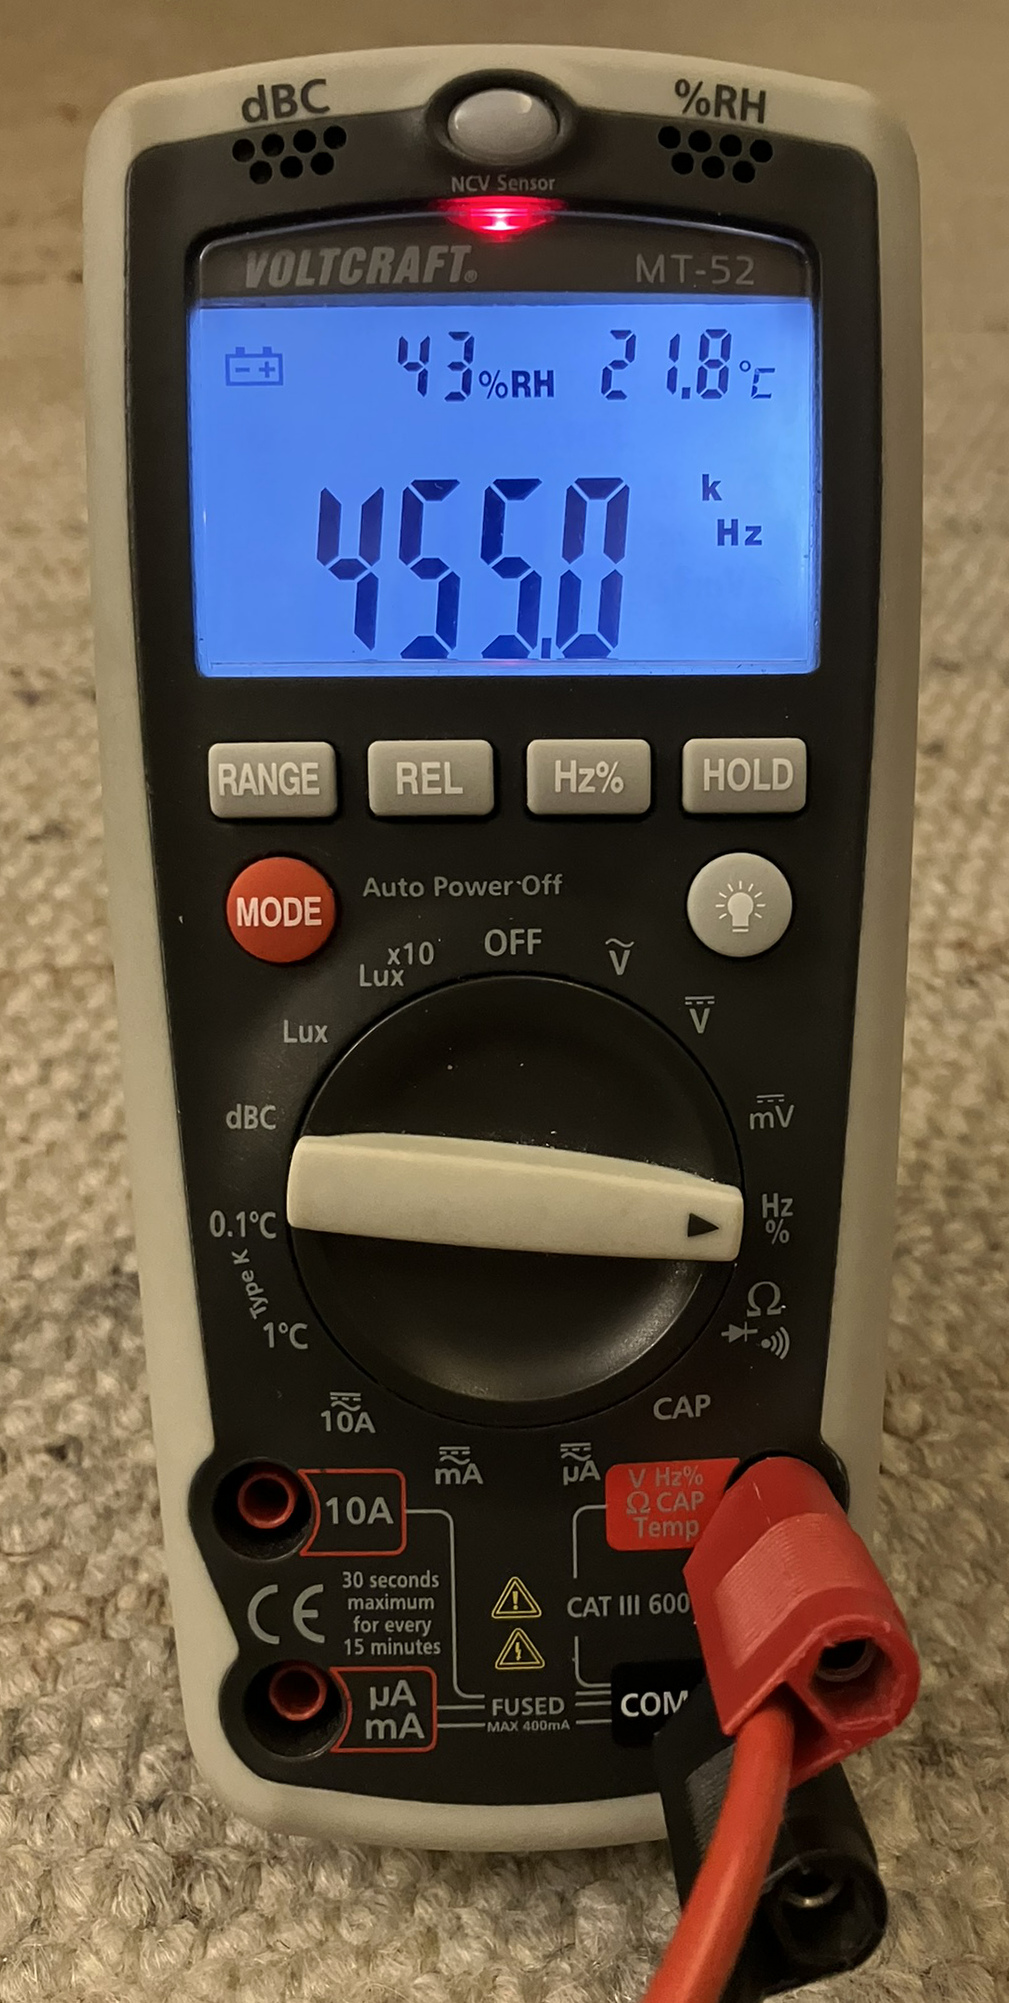
\includegraphics[width=0.85\textwidth]{foto/189}
    \caption{\scriptsize Multimeter, das im Frequenzmessbereich \qty{455}{\kilo\hertz} anzeigt. Darüber erscheinen ein Symbol für niedrige Batteriespannung, die Luftfeuchtigkeit und die Temperatur. Diese Werte haben nichts mit der Frequenzmessung zu tun.}
    \label{e_frequenzzaehler2}
\end{figure}

   \end{column}
\end{columns}

\end{frame}

\begin{frame}
\only<1>{
\begin{QQuestion}{EI501}{Womit kann die Frequenz eines unmodulierten Hochfrequenzsignals gemessen werden? Mit einem~...}{Frequenzzähler.}
{Widerstandsmessgerät.}
{Wechselspannungsmessgerät.}
{Wechselstromzähler.}
\end{QQuestion}

}
\only<2>{
\begin{QQuestion}{EI501}{Womit kann die Frequenz eines unmodulierten Hochfrequenzsignals gemessen werden? Mit einem~...}{\textbf{\textcolor{DARCgreen}{Frequenzzähler.}}}
{Widerstandsmessgerät.}
{Wechselspannungsmessgerät.}
{Wechselstromzähler.}
\end{QQuestion}

}
\end{frame}

\begin{frame}
\begin{columns}
    \begin{column}{0.48\textwidth}
    \begin{itemize}
  \item Anzeige der Frequenz
  \item Bei älteren Geräten steht hinten ein 10<sup>x</sup>-Multiplikator
  \end{itemize}

    \end{column}
   \begin{column}{0.48\textwidth}
       
\begin{figure}
    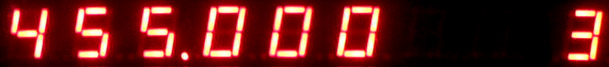
\includegraphics[width=0.85\textwidth]{foto/187}
    \caption{\scriptsize Display eines Frequenzzählers, der 455 · 10<sup>3</sup> Hz anzeigt}
    \label{e_frequenzzaehler1}
\end{figure}

   \end{column}
\end{columns}

\end{frame}

\begin{frame}
\begin{columns}
    \begin{column}{0.48\textwidth}
    \begin{itemize}
  \item Abgleichanleitung verlangt oft Einstellung bis auf eine bestimmte Abweichung
  \item z.B.  $\pm$ 10 Hz
  \item Stellenwert der Ziffern kennen
  \item Auf Komma und Einheitenpräfix oder Multiplikator achten
  \end{itemize}

    \end{column}
   \begin{column}{0.48\textwidth}
       
\begin{figure}
    \DARCimage{0.85\linewidth}{793include}
    \caption{\scriptsize Diese Anzeige stellt eine Frequenz in MHz dar. Das ist zugleich der Stellenwert der Ziffer vor dem Komma.}
    \label{e_frequenzzaehler_stellen}
\end{figure}


\begin{figure}
    \DARCimage{0.85\linewidth}{104include}
    \caption{\scriptsize Manche Anzeigen eines Frequenzzählers haben weniger Nachkommastellen}
    \label{e_frequenzzaehler_weniger_stellen}
\end{figure}


   \end{column}
\end{columns}

\end{frame}

\begin{frame}
\only<1>{
\begin{PQuestion}{EI502}{Das Bild stellt die Anzeige eines Frequenzzählers dar. Welchen Stellenwert hat die mit X gekennzeichnete Ziffer?}{ein Kilohertz}
{ein Hertz}
{hundert Hertz}
{zehn Hertz}
{\DARCimage{1.0\linewidth}{103include}}\end{PQuestion}

}
\only<2>{
\begin{PQuestion}{EI502}{Das Bild stellt die Anzeige eines Frequenzzählers dar. Welchen Stellenwert hat die mit X gekennzeichnete Ziffer?}{\textbf{\textcolor{DARCgreen}{ein Kilohertz}}}
{ein Hertz}
{hundert Hertz}
{zehn Hertz}
{\DARCimage{1.0\linewidth}{103include}}\end{PQuestion}

}
\end{frame}

\begin{frame}
\only<1>{
\begin{PQuestion}{EI503}{Das Bild stellt die Anzeige eines Frequenzzählers dar. Welchen Stellenwert hat die mit X gekennzeichnete Ziffer?}{ein Kilohertz}
{ein Hertz}
{hundert Hertz}
{zehn Hertz}
{\DARCimage{1.0\linewidth}{104include}}\end{PQuestion}

}
\only<2>{
\begin{PQuestion}{EI503}{Das Bild stellt die Anzeige eines Frequenzzählers dar. Welchen Stellenwert hat die mit X gekennzeichnete Ziffer?}{ein Kilohertz}
{ein Hertz}
{hundert Hertz}
{\textbf{\textcolor{DARCgreen}{zehn Hertz}}}
{\DARCimage{1.0\linewidth}{104include}}\end{PQuestion}

}
\end{frame}

\begin{frame}
\frametitle{Wertebereich}
\begin{itemize}
  \item Außerhalb des angegebenen Wertebereichs messen Frequenzzähler ungenau oder gar nicht
  \item Für höhere Frequenzen gibt es Frequenzteiler
  \item Angelegte Frequenz wird durch einen festen Wert geteilt
  \item Ergebnis wird als elektrische Schwingung ausgegeben
  \item \emph{Vorteiler} genannt, da zwischen Messobjekt und Zähler geschaltet
  \item 10:1-Teiler bei \qty{2,4}{\giga\hertz} $\rightarrow$ \qty{240}{\mega\hertz}
  \end{itemize}
\end{frame}

\begin{frame}
\only<1>{
\begin{QQuestion}{EI504}{Wenn ein 10:1-Frequenzteiler vor einem Frequenzzähler geschaltet wird und der Zähler \qty{14,5625}{\MHz} anzeigt, beträgt die tatsächliche Frequenz~...}{\qty{14,5625}{\kHz}.}
{\qty{1,45625}{\MHz}.}
{\qty{14,5625}{\MHz}.}
{\qty{145,625}{\MHz}.}
\end{QQuestion}

}
\only<2>{
\begin{QQuestion}{EI504}{Wenn ein 10:1-Frequenzteiler vor einem Frequenzzähler geschaltet wird und der Zähler \qty{14,5625}{\MHz} anzeigt, beträgt die tatsächliche Frequenz~...}{\qty{14,5625}{\kHz}.}
{\qty{1,45625}{\MHz}.}
{\qty{14,5625}{\MHz}.}
{\textbf{\textcolor{DARCgreen}{\qty{145,625}{\MHz}.}}}
\end{QQuestion}

}
\end{frame}%ENDCONTENT


\title{DARC Amateurfunklehrgang Klasse E}
\author{Sender}
\institute{Deutscher Amateur Radio Club e.\,V.}
\begin{frame}
\maketitle
\end{frame}

\section{ALC}
\label{section:alc}
\begin{frame}%STARTCONTENT
\begin{itemize}
  \item \emph{Automatic-Level-Control (ALC)} regelt die Aussteuerung der Senderendstufe
  \item Reduziert bei Übersteuerung die Amplitude im Sendezweig
  \item Nicht verwechseln mit der AGC (Automatic-Gain-Control) im Empfängerzweig
  \end{itemize}
\end{frame}

\begin{frame}
\frametitle{Funktionsweise}
\begin{itemize}
  \item Erfassung der Ausgangsleistung und Vergleich mit vorgegebenen maximalen Wert
  \item Bei Überschreiten wird eine Regelspannung an vorgelagerte HF-Verstärkerstufe gegeben
  \item Amplitude des Sendesignals wird reduziert
  \end{itemize}
\end{frame}

\begin{frame}\begin{itemize}
  \item Wenn ALC-Anzeige anspricht, ist Sender durch zu starkes NF-Signal übersteuert
  \item Bei SSB ist ein geringfügiges Übersteuern erwünscht
  \item Gleicht Lautstärkeschwankungen in der Stimme aus
  \item ALC-Anzeige ist deshalb oft ein Balken
  \end{itemize}
\end{frame}

\begin{frame}\begin{itemize}
  \item Bei Digimodes sollte die ALC nicht ansprechen
  \item Verzerrung des Sendesignals
  \item NF-Signal so weit aussteuern, dass ALC gerade nicht anspricht
  \end{itemize}
\end{frame}

\begin{frame}
\only<1>{
\begin{QQuestion}{EF305}{Was bewirkt die ALC (Automatic Level Control) bei zu starkem NF-Signal in einem Transceiver?}{Sie reduziert die Amplitude des Signals im Sendezweig vor dem Leistungsverstärker.}
{Sie erhöht die Amplitude des Signals im Sendezweig vor dem Leistungsverstärker.}
{Sie reduziert die Verstärkung von Verstärkerstufen im Empfangsteil.}
{Sie erhöht die Verstärkung von Verstärkerstufen im Empfangsteil.}
\end{QQuestion}

}
\only<2>{
\begin{QQuestion}{EF305}{Was bewirkt die ALC (Automatic Level Control) bei zu starkem NF-Signal in einem Transceiver?}{\textbf{\textcolor{DARCgreen}{Sie reduziert die Amplitude des Signals im Sendezweig vor dem Leistungsverstärker.}}}
{Sie erhöht die Amplitude des Signals im Sendezweig vor dem Leistungsverstärker.}
{Sie reduziert die Verstärkung von Verstärkerstufen im Empfangsteil.}
{Sie erhöht die Verstärkung von Verstärkerstufen im Empfangsteil.}
\end{QQuestion}

}
\end{frame}%ENDCONTENT


\section{Senderausgangsleistung}
\label{section:senderausgangsleistung}
\begin{frame}%STARTCONTENT
\begin{itemize}
  \item Verpflichtung von Funkamateuren die Leistungsgrenzwerte ihrer Funkanlage einzuhalten
  \item Auf vielen Amateurfunkbändern gilt eine \emph{maximale Senderausgangsleistung} (\emph{PEP}, Peak-Envelope-Power) als Grenzwert
  \item Auch unerwünschte Aussendungen sind von Bedeutung
  \end{itemize}
\end{frame}

\begin{frame}
\frametitle{Messung von unerwünschten Aussendungen}
\begin{itemize}
  \item Am Senderausgang
  \item Unter Einzebiehung von Stehwellenmessgerät, Anpassgerät(e), Tiefpassfilter etc.
  \item Messsung von unerwünschen Aussendungen, die die Antenne erreichen können
  \end{itemize}
\end{frame}

\begin{frame}
\only<1>{
\begin{QQuestion}{EJ209}{Wie erfolgt die Messung der Leistungen, die zu unerwünschten Aussendungen führen?}{Die Messung erfolgt am Senderausgang mit einem hochohmigen HF-Tastkopf und angeschlossenem Transistorvoltmeter.}
{Die Messung erfolgt am Fußpunkt der im Funkbetrieb verwendeten Antenne unter Einbeziehung des gegebenenfalls verwendeten Antennenanpassgeräts.}
{Die Messung erfolgt am Ausgang der Antennenleitung unter Einbeziehung des im Funkbetrieb verwendeten Antennenanpassgeräts.}
{Die Messung erfolgt am Senderausgang unter Einbeziehung des gegebenenfalls verwendeten Stehwellenmessgeräts und des gegebenenfalls verwendeten Tiefpassfilters.}
\end{QQuestion}

}
\only<2>{
\begin{QQuestion}{EJ209}{Wie erfolgt die Messung der Leistungen, die zu unerwünschten Aussendungen führen?}{Die Messung erfolgt am Senderausgang mit einem hochohmigen HF-Tastkopf und angeschlossenem Transistorvoltmeter.}
{Die Messung erfolgt am Fußpunkt der im Funkbetrieb verwendeten Antenne unter Einbeziehung des gegebenenfalls verwendeten Antennenanpassgeräts.}
{Die Messung erfolgt am Ausgang der Antennenleitung unter Einbeziehung des im Funkbetrieb verwendeten Antennenanpassgeräts.}
{\textbf{\textcolor{DARCgreen}{Die Messung erfolgt am Senderausgang unter Einbeziehung des gegebenenfalls verwendeten Stehwellenmessgeräts und des gegebenenfalls verwendeten Tiefpassfilters.}}}
\end{QQuestion}

}
\end{frame}

\begin{frame}
\frametitle{Messung der Senderausgangsleistung}
\begin{itemize}
  \item Direkt am Senderausgang
  \item Ohne Zusatzgeräte, Filter oder Kabel
  \item Bei SSB $\rightarrow$ mit Modulation
  \item Ein- oder Zweitonaussteuerung, aber keine Sprache
  \item Messung der maximalen \emph{Hüllkurvenleistung} (PEP)
  \item Spitzenleistung des Senders bei maximaler Aussteuerung
  \end{itemize}

\end{frame}

\begin{frame}
\only<1>{
\begin{QQuestion}{EF401}{Die Ausgangsleistung eines Senders ist die unmittelbar nach~...}{dem Senderausgang gemessene Summe aus vorlaufender und rücklaufender Leistung.}
{dem Senderausgang gemessene Differenz aus vorlaufender und rücklaufender Leistung.}
{der Antenne messbaren Leistung, die durch ein Feldstärkenmessgerät im Nahfeld ermittelt werden kann.}
{dem Senderausgang messbare Leistung, bevor sie Zusatzgeräte durchläuft.}
\end{QQuestion}

}
\only<2>{
\begin{QQuestion}{EF401}{Die Ausgangsleistung eines Senders ist die unmittelbar nach~...}{dem Senderausgang gemessene Summe aus vorlaufender und rücklaufender Leistung.}
{dem Senderausgang gemessene Differenz aus vorlaufender und rücklaufender Leistung.}
{der Antenne messbaren Leistung, die durch ein Feldstärkenmessgerät im Nahfeld ermittelt werden kann.}
{\textbf{\textcolor{DARCgreen}{dem Senderausgang messbare Leistung, bevor sie Zusatzgeräte durchläuft.}}}
\end{QQuestion}

}
\end{frame}

\begin{frame}
\only<1>{
\begin{QQuestion}{EF402}{Wie und wo wird die Ausgangsleistung eines SSB-Senders gemessen? Die maximale Hüllkurvenleistung (PEP) wird gemessen...}{zwischen Antennentuner und Speisepunkt bei Sprachmodulation.}
{zwischen Antennentuner und Speisepunkt der Antenne mit unmoduliertem Träger.}
{direkt am Senderausgang bei Ein- oder Zweitonaussteuerung.}
{direkt am Senderausgang mit unmoduliertem Träger.}
\end{QQuestion}

}
\only<2>{
\begin{QQuestion}{EF402}{Wie und wo wird die Ausgangsleistung eines SSB-Senders gemessen? Die maximale Hüllkurvenleistung (PEP) wird gemessen...}{zwischen Antennentuner und Speisepunkt bei Sprachmodulation.}
{zwischen Antennentuner und Speisepunkt der Antenne mit unmoduliertem Träger.}
{\textbf{\textcolor{DARCgreen}{direkt am Senderausgang bei Ein- oder Zweitonaussteuerung.}}}
{direkt am Senderausgang mit unmoduliertem Träger.}
\end{QQuestion}

}
\end{frame}%ENDCONTENT


\section{Unerwünschte Aussendungen II}
\label{section:unerwuenschte_aussendungen_2}
\begin{frame}%STARTCONTENT

\frametitle{Oberwellen}
\begin{itemize}
  \item Ganzzahlige Vielfache der Grundfrequenz
  \item Entstehen durch Signalformen, die nicht sinusförmig sind, insbesondere bei Übersteuerung
  \item Beeinträchtigung anderer Funkdienste
  \item Können reduziert werden
  \end{itemize}
\end{frame}

\begin{frame}
\only<1>{
\begin{QQuestion}{EJ201}{Welche Signalform sollte der Träger einer hochfrequenten Schwingung haben, um Störungen durch Oberwellen zu vermeiden?}{kreisförmig}
{rechteckförmig}
{dreieckförmig}
{sinusförmig}
\end{QQuestion}

}
\only<2>{
\begin{QQuestion}{EJ201}{Welche Signalform sollte der Träger einer hochfrequenten Schwingung haben, um Störungen durch Oberwellen zu vermeiden?}{kreisförmig}
{rechteckförmig}
{dreieckförmig}
{\textbf{\textcolor{DARCgreen}{sinusförmig}}}
\end{QQuestion}

}
\end{frame}

\begin{frame}
\only<1>{
\begin{QQuestion}{EJ202}{Wie kann man hochfrequente Störungen reduzieren, die durch Harmonische hervorgerufen werden? Sie können reduziert werden durch ein~...}{ZF-Filter.}
{Nachbarkanalfilter.}
{Oberwellenfilter.}
{Hochpassfilter.}
\end{QQuestion}

}
\only<2>{
\begin{QQuestion}{EJ202}{Wie kann man hochfrequente Störungen reduzieren, die durch Harmonische hervorgerufen werden? Sie können reduziert werden durch ein~...}{ZF-Filter.}
{Nachbarkanalfilter.}
{\textbf{\textcolor{DARCgreen}{Oberwellenfilter.}}}
{Hochpassfilter.}
\end{QQuestion}

}
\end{frame}

\begin{frame}
\frametitle{Tiefpassfilter}
\begin{columns}
    \begin{column}{0.48\textwidth}
    \begin{itemize}
  \item Nur Frequenzen unterhalb einer bestimmten Grenzfrequenz werden durchgelassen
  \item Oberwellen können nicht passieren oder werden stark abgeschwächt
  \end{itemize}

    \end{column}
   \begin{column}{0.48\textwidth}
         
\begin{figure}
    \DARCimage{0.85\linewidth}{591include}
    \caption{\scriptsize Frequenzgang eines Tiefpassfilters}
    \label{tiefpass}
\end{figure}


   \end{column}
\end{columns}

\end{frame}

\begin{frame}
\only<1>{
\begin{QQuestion}{EJ204}{Welches Filter wäre zwischen Senderausgang und Antenne eingeschleift am besten zur Verringerung der Oberwellenausstrahlungen geeignet?}{Ein Antennenfilter}
{Ein Hochpassfilter}
{Ein Tiefpassfilter}
{Ein Sperrkreisfilter}
\end{QQuestion}

}
\only<2>{
\begin{QQuestion}{EJ204}{Welches Filter wäre zwischen Senderausgang und Antenne eingeschleift am besten zur Verringerung der Oberwellenausstrahlungen geeignet?}{Ein Antennenfilter}
{Ein Hochpassfilter}
{\textbf{\textcolor{DARCgreen}{Ein Tiefpassfilter}}}
{Ein Sperrkreisfilter}
\end{QQuestion}

}
\end{frame}

\begin{frame}
\only<1>{
\begin{QQuestion}{EJ205}{Um Oberwellenaussendungen eines UHF-Senders zu minimieren, sollte dem Gerät~...}{ein Notchfilter vorgeschaltet werden.}
{ein Hochpassfilter nachgeschaltet werden.}
{eine Bandsperre vorgeschaltet werden.}
{ein Tiefpassfilter nachgeschaltet werden.}
\end{QQuestion}

}
\only<2>{
\begin{QQuestion}{EJ205}{Um Oberwellenaussendungen eines UHF-Senders zu minimieren, sollte dem Gerät~...}{ein Notchfilter vorgeschaltet werden.}
{ein Hochpassfilter nachgeschaltet werden.}
{eine Bandsperre vorgeschaltet werden.}
{\textbf{\textcolor{DARCgreen}{ein Tiefpassfilter nachgeschaltet werden.}}}
\end{QQuestion}

}
\end{frame}

\begin{frame}
\only<1>{
\begin{question2x2}{EJ206}{Welche Schaltung wäre, zwischen Senderausgang und Antenne eingeschleift, am besten zur Verringerung der Oberwellenausstrahlungen geeignet?}{\DARCimage{1.0\linewidth}{161include}}
{\DARCimage{1.0\linewidth}{167include}}
{\DARCimage{1.0\linewidth}{165include}}
{\DARCimage{1.0\linewidth}{168include}}
\end{question2x2}

}
\only<2>{
\begin{question2x2}{EJ206}{Welche Schaltung wäre, zwischen Senderausgang und Antenne eingeschleift, am besten zur Verringerung der Oberwellenausstrahlungen geeignet?}{\DARCimage{1.0\linewidth}{161include}}
{\textbf{\textcolor{DARCgreen}{\DARCimage{1.0\linewidth}{167include}}}}
{\DARCimage{1.0\linewidth}{165include}}
{\DARCimage{1.0\linewidth}{168include}}
\end{question2x2}

}
\end{frame}

\begin{frame}
\only<1>{
\begin{question2x2}{EJ207}{Welche Charakteristik sollte ein Filter zur Verringerung der Oberwellen eines KW-Senders haben?}{\DARCimage{0.75\linewidth}{250include}}
{\DARCimage{0.75\linewidth}{251include}}
{\DARCimage{0.75\linewidth}{258include}}
{\DARCimage{0.75\linewidth}{259include}}
\end{question2x2}

}
\only<2>{
\begin{question2x2}{EJ207}{Welche Charakteristik sollte ein Filter zur Verringerung der Oberwellen eines KW-Senders haben?}{\textbf{\textcolor{DARCgreen}{\DARCimage{0.75\linewidth}{250include}}}}
{\DARCimage{0.75\linewidth}{251include}}
{\DARCimage{0.75\linewidth}{258include}}
{\DARCimage{0.75\linewidth}{259include}}
\end{question2x2}

}
\end{frame}

\begin{frame}
\only<1>{
\begin{question2x2}{EJ208}{Welche Filtercharakteristik würde sich am besten für den Ausgang eines KW-Mehrband-Senders eignen?}{\DARCimage{0.75\linewidth}{252include}}
{\DARCimage{0.75\linewidth}{251include}}
{\DARCimage{0.75\linewidth}{250include}}
{\DARCimage{0.75\linewidth}{253include}}
\end{question2x2}

}
\only<2>{
\begin{question2x2}{EJ208}{Welche Filtercharakteristik würde sich am besten für den Ausgang eines KW-Mehrband-Senders eignen?}{\DARCimage{0.75\linewidth}{252include}}
{\DARCimage{0.75\linewidth}{251include}}
{\textbf{\textcolor{DARCgreen}{\DARCimage{0.75\linewidth}{250include}}}}
{\DARCimage{0.75\linewidth}{253include}}
\end{question2x2}

}
\end{frame}

\begin{frame}
\only<1>{
\begin{QQuestion}{EJ203}{Was für ein Filter muss zwischen Transceiver und Antennenzuleitung eingefügt werden, um Oberwellen zu reduzieren?}{Hochpassfilter}
{Tiefpassfilter}
{CW-Filter}
{NF-Filter}
\end{QQuestion}

}
\only<2>{
\begin{QQuestion}{EJ203}{Was für ein Filter muss zwischen Transceiver und Antennenzuleitung eingefügt werden, um Oberwellen zu reduzieren?}{Hochpassfilter}
{\textbf{\textcolor{DARCgreen}{Tiefpassfilter}}}
{CW-Filter}
{NF-Filter}
\end{QQuestion}

}
\end{frame}

\begin{frame}
\frametitle{Hochpassfilter}
\begin{columns}
    \begin{column}{0.48\textwidth}
    \begin{itemize}
  \item Nur Frequenzen oberhalb einer bestimmten Grenzfrequenz werden durchgelassen
  \item Werden im Empfängereingang verwendet, damit tiefe Frequenzen nicht stören
  \end{itemize}

    \end{column}
   \begin{column}{0.48\textwidth}
          
\begin{figure}
    \DARCimage{0.85\linewidth}{592include}
    \caption{\scriptsize Frequenzgang eines Hochpassfilters}
    \label{hochpass}
\end{figure}


   \end{column}
\end{columns}

\end{frame}

\begin{frame}
\frametitle{Bandpassfilter}
\begin{columns}
    \begin{column}{0.48\textwidth}
    \begin{itemize}
  \item Bei Einbandsendern
  \item Sender im VHF/UHF/SHF-Bereich
  \item Signale aus der Signalaufbereitung unterhalb der Sendefrequenz unterdrücken
  \end{itemize}

    \end{column}
   \begin{column}{0.48\textwidth}
          
\begin{figure}
    \DARCimage{0.85\linewidth}{593include}
    \caption{\scriptsize Frequenzgang eines Bandpassfilters}
    \label{bandpass}
\end{figure}


   \end{column}
\end{columns}

\end{frame}

\begin{frame}
\frametitle{Arbeitspunkt}
\begin{itemize}
  \item Sender-Stufen und Leistungs-Endstufen sollen verzerrungsfrei arbeiten
  \item Nach Veränderung des Arbeitspunkts auf Linearität (saubere Sinus-Verstärkung) prüfen
  \item Aussendung auf Oberwellen prüfen
  \end{itemize}
\end{frame}

\begin{frame}
\only<1>{
\begin{QQuestion}{EF404}{Wann sollte ein Sender auf mögliche Oberwellenaussendungen überprüft werden?}{Vor jedem Sendebetrieb.
}
{Bei Empfang eines Störsignals.}
{Wenn der Arbeitspunkt der Endstufe neu justiert wurde.
}
{Wenn Splatter-Störungen zu hören sind.}
\end{QQuestion}

}
\only<2>{
\begin{QQuestion}{EF404}{Wann sollte ein Sender auf mögliche Oberwellenaussendungen überprüft werden?}{Vor jedem Sendebetrieb.
}
{Bei Empfang eines Störsignals.}
{\textbf{\textcolor{DARCgreen}{Wenn der Arbeitspunkt der Endstufe neu justiert wurde.
}}}
{Wenn Splatter-Störungen zu hören sind.}
\end{QQuestion}

}
\end{frame}%ENDCONTENT


\section{Störungen elektronischer Geräte I}
\label{section:stoerungen_elektronischer_geraete_1}
\begin{frame}%STARTCONTENT
\begin{itemize}
  \item Starke Sender führen zu unterschiedlichen Störungen und Beeinflussungen von elektronischen Geräten und Anlagen
  \item Ziel: Störungen vermeiden oder Ursachen durch Gegenmaßnahmen beseitigen
  \end{itemize}
\end{frame}

\begin{frame}
\frametitle{Einströmung}
\begin{itemize}
  \item Hochfrequenz gelangt durch Leitungen oder Kabel in ein Gerät
  \item Zum Beispiel über die Netzleitung, Antennenleitung, Lautsprecherkabel
  \end{itemize}
\end{frame}

\begin{frame}
\only<1>{
\begin{QQuestion}{EJ101}{In welchem Fall spricht man von Einströmungen? Einströmungen liegen dann vor, wenn Hochfrequenz~...}{wegen eines schlechten Stehwellenverhältnisses wieder zum Sender zurück strömt.}
{über das ungenügend abgeschirmte Gehäuse in die Elektronik gelangt.}
{über nicht genügend geschirmte Kabel zum Anpassgerät geführt wird.}
{über Leitungen oder Kabel in ein Gerät gelangt.}
\end{QQuestion}

}
\only<2>{
\begin{QQuestion}{EJ101}{In welchem Fall spricht man von Einströmungen? Einströmungen liegen dann vor, wenn Hochfrequenz~...}{wegen eines schlechten Stehwellenverhältnisses wieder zum Sender zurück strömt.}
{über das ungenügend abgeschirmte Gehäuse in die Elektronik gelangt.}
{über nicht genügend geschirmte Kabel zum Anpassgerät geführt wird.}
{\textbf{\textcolor{DARCgreen}{über Leitungen oder Kabel in ein Gerät gelangt.}}}
\end{QQuestion}

}
\end{frame}

\begin{frame}
\frametitle{Einstrahlung}
\begin{itemize}
  \item Hochfrequenz gelangt wegen ungenügend geschirmten Gehäuse in die Elektronik
  \item Führt dort zu Störungen
  \end{itemize}
\end{frame}

\begin{frame}
\only<1>{
\begin{QQuestion}{EJ102}{In welchem Fall spricht man von Einstrahlungen bei EMV? Einstrahlungen liegen dann vor, wenn die Hochfrequenz~...}{über das ungenügend abgeschirmte Gehäuse in die Elektronik gelangt.}
{über Leitungen oder Kabel in das gestörte Gerät gelangt.}
{über nicht genügend geschirmte Kabel zum gestörten Empfänger gelangt.}
{wegen eines schlechten Stehwellenverhältnisses wieder zum Sender zurück strahlt.}
\end{QQuestion}

}
\only<2>{
\begin{QQuestion}{EJ102}{In welchem Fall spricht man von Einstrahlungen bei EMV? Einstrahlungen liegen dann vor, wenn die Hochfrequenz~...}{\textbf{\textcolor{DARCgreen}{über das ungenügend abgeschirmte Gehäuse in die Elektronik gelangt.}}}
{über Leitungen oder Kabel in das gestörte Gerät gelangt.}
{über nicht genügend geschirmte Kabel zum gestörten Empfänger gelangt.}
{wegen eines schlechten Stehwellenverhältnisses wieder zum Sender zurück strahlt.}
\end{QQuestion}

}
\end{frame}

\begin{frame}
\frametitle{Störende Beeinflussung}
\begin{itemize}
  \item Kann trotz gesetzeskonformen Betrieb eines Senders beim Empfänger in Nähe auftreten
  \item Garagentorsteuerungen oder Funk-Autoschlüssel funktionieren nicht mehr wie gewohnt
  \item Störung von LED-Leuchten
  \end{itemize}
\end{frame}

\begin{frame}
\only<1>{
\begin{QQuestion}{EJ103}{Bereits durch die Aussendung des reinen Nutzsignals können in benachbarten Empfängern Störungen beim Empfang anderer Frequenzen auftreten. Dabei handelt es sich um eine~...}{Übersteuerung oder störende Beeinflussung.}
{Störung durch unerwünschte Aussendungen.}
{Störung durch unerwünschte Nebenaussendungen.}
{hinzunehmende Störung.}
\end{QQuestion}

}
\only<2>{
\begin{QQuestion}{EJ103}{Bereits durch die Aussendung des reinen Nutzsignals können in benachbarten Empfängern Störungen beim Empfang anderer Frequenzen auftreten. Dabei handelt es sich um eine~...}{\textbf{\textcolor{DARCgreen}{Übersteuerung oder störende Beeinflussung.}}}
{Störung durch unerwünschte Aussendungen.}
{Störung durch unerwünschte Nebenaussendungen.}
{hinzunehmende Störung.}
\end{QQuestion}

}
\end{frame}

\begin{frame}
\only<1>{
\begin{QQuestion}{EJ112}{Welches Gerät kann durch Aussendungen eines Amateurfunksenders störende Beeinflussungen zeigen?}{LED-Lampe mit Netzanschluss}
{Dampfbügeleisen mit Bimetall-Temperaturregler}
{Staubsauger mit Kollektormotor}
{Antennenrotor mit Wechselstrommotor}
\end{QQuestion}

}
\only<2>{
\begin{QQuestion}{EJ112}{Welches Gerät kann durch Aussendungen eines Amateurfunksenders störende Beeinflussungen zeigen?}{\textbf{\textcolor{DARCgreen}{LED-Lampe mit Netzanschluss}}}
{Dampfbügeleisen mit Bimetall-Temperaturregler}
{Staubsauger mit Kollektormotor}
{Antennenrotor mit Wechselstrommotor}
\end{QQuestion}

}
\end{frame}

\begin{frame}
\only<1>{
\begin{QQuestion}{EJ113}{Wie kommen Geräusche aus den Lautsprechern einer abgeschalteten Stereoanlage möglicherweise zustande?}{Durch Gleichrichtung starker HF-Signale in der NF-Endstufe der Stereoanlage.}
{Durch Gleichrichtung der ins Stromnetz eingestrahlten HF-Signale an den Dioden des Netzteils.}
{Durch Gleichrichtung abgestrahlter HF-Signale an PN-Übergängen in der NF-Vorstufe.}
{Durch eine Übersteuerung des Tuners mit dem über die Antennenzuleitung aufgenommenen HF-Signal.}
\end{QQuestion}

}
\only<2>{
\begin{QQuestion}{EJ113}{Wie kommen Geräusche aus den Lautsprechern einer abgeschalteten Stereoanlage möglicherweise zustande?}{\textbf{\textcolor{DARCgreen}{Durch Gleichrichtung starker HF-Signale in der NF-Endstufe der Stereoanlage.}}}
{Durch Gleichrichtung der ins Stromnetz eingestrahlten HF-Signale an den Dioden des Netzteils.}
{Durch Gleichrichtung abgestrahlter HF-Signale an PN-Übergängen in der NF-Vorstufe.}
{Durch eine Übersteuerung des Tuners mit dem über die Antennenzuleitung aufgenommenen HF-Signal.}
\end{QQuestion}

}
\end{frame}

\begin{frame}
\frametitle{Intermodulation}
\begin{itemize}
  \item Beim Auftreten von mehreren starken Empfangssignalen
  \item Z.B. TV-Sender und starke Amateurfunkstation in der Nachbarschaft
  \item Führt zu unerwünschten Oberwellen und deren Mischprodukten
  \item Durch Intermodulation werden Phantomsignale hervorgerufen
  \end{itemize}
\end{frame}

\begin{frame}
\only<1>{
\begin{QQuestion}{EJ120}{Welche Empfangs-Effekte werden durch Intermodulation hervorgerufen?}{Dem Empfangssignal ist ein pulsierendes Rauschen überlagert, das die Verständlichkeit beeinträchtigt.}
{Das Nutzsignal wird mit einem anderen Signal moduliert und dadurch verständlicher.}
{Es treten Phantomsignale auf, die selbst bei Einschalten eines Abschwächers in den HF-Signalweg nicht verschwinden.}
{Es treten Phantomsignale auf, die bei Abschalten einer der beteiligten Mischfrequenzen verschwindet.}
\end{QQuestion}

}
\only<2>{
\begin{QQuestion}{EJ120}{Welche Empfangs-Effekte werden durch Intermodulation hervorgerufen?}{Dem Empfangssignal ist ein pulsierendes Rauschen überlagert, das die Verständlichkeit beeinträchtigt.}
{Das Nutzsignal wird mit einem anderen Signal moduliert und dadurch verständlicher.}
{Es treten Phantomsignale auf, die selbst bei Einschalten eines Abschwächers in den HF-Signalweg nicht verschwinden.}
{\textbf{\textcolor{DARCgreen}{Es treten Phantomsignale auf, die bei Abschalten einer der beteiligten Mischfrequenzen verschwindet.}}}
\end{QQuestion}

}
\end{frame}

\begin{frame}
\frametitle{Oxidation}
\begin{itemize}
  \item Korrodierte Kontakte (Metall-Oxide) zwischen Metallen bilden Nichtlinearitäten durch Gleichricht-Effekte
  \item Unerwünschte Mischprodukte auf der Sende- und Empfangsseite
  \item Kann zu Störungen im Fernseh- und Rundfunkempfang führen
  \end{itemize}
\end{frame}

\begin{frame}
\only<1>{
\begin{QQuestion}{EJ121}{Ein korrodierter Anschluss an der Fernseh-Empfangsantenne des Nachbarn kann in Verbindung mit~...}{ dem Signal naher Sender unerwünschte Mischprodukte erzeugen, die den Fernsehempfang stören.}
{ dem Oszillatorsignal des Fernsehempfängers unerwünschte Mischprodukte erzeugen, die den Fernsehempfang stören.}
{ Einstreuungen aus dem Stromnetz durch Intermodulation Bild- und Tonstörungen hervorrufen.}
{dem Signal naher Sender parametrische Schwingungen erzeugen, die einen überhöhten Nutzsignalpegel hervorrufen.}
\end{QQuestion}

}
\only<2>{
\begin{QQuestion}{EJ121}{Ein korrodierter Anschluss an der Fernseh-Empfangsantenne des Nachbarn kann in Verbindung mit~...}{\textbf{\textcolor{DARCgreen}{ dem Signal naher Sender unerwünschte Mischprodukte erzeugen, die den Fernsehempfang stören.}}}
{ dem Oszillatorsignal des Fernsehempfängers unerwünschte Mischprodukte erzeugen, die den Fernsehempfang stören.}
{ Einstreuungen aus dem Stromnetz durch Intermodulation Bild- und Tonstörungen hervorrufen.}
{dem Signal naher Sender parametrische Schwingungen erzeugen, die einen überhöhten Nutzsignalpegel hervorrufen.}
\end{QQuestion}

}
\end{frame}

\begin{frame}
\frametitle{Erforderliche Sendeleistung}
\begin{itemize}
  \item Stets nur die für eine zufriedenstellende Kommunikation erforderliche Sendeleistung verwenden
  \item Zur Vermeidung von Störungen von Geräten
  \end{itemize}
\end{frame}

\begin{frame}
\only<1>{
\begin{QQuestion}{EJ104}{Um die Störwahrscheinlichkeit zu verringern, sollte die benutzte Sendeleistung~...}{nur auf den zulässigen Pegel eingestellt werden.}
{auf das für eine zufriedenstellende Kommunikation erforderliche Minimum eingestellt werden.}
{auf die für eine zufriedenstellende Kommunikation erforderlichen \qty{100}{\W} eingestellt werden.}
{die Hälfte des maximal zulässigen Pegels betragen.}
\end{QQuestion}

}
\only<2>{
\begin{QQuestion}{EJ104}{Um die Störwahrscheinlichkeit zu verringern, sollte die benutzte Sendeleistung~...}{nur auf den zulässigen Pegel eingestellt werden.}
{\textbf{\textcolor{DARCgreen}{auf das für eine zufriedenstellende Kommunikation erforderliche Minimum eingestellt werden.}}}
{auf die für eine zufriedenstellende Kommunikation erforderlichen \qty{100}{\W} eingestellt werden.}
{die Hälfte des maximal zulässigen Pegels betragen.}
\end{QQuestion}

}
\end{frame}

\begin{frame}
\only<1>{
\begin{QQuestion}{EJ105}{Bei einem Wohnort in einem Ballungsgebiet empfiehlt es sich, während der abendlichen Fernsehstunden~...}{mit keiner höheren Leistung zu senden, als für eine sichere Kommunikation erforderlich ist.}
{nur mit effektiver Leistung zu senden.}
{nur mit einer Hochgewinn-Richtantenne zu senden.}
{die Antenne unterhalb der Dachhöhe herabzulassen.}
\end{QQuestion}

}
\only<2>{
\begin{QQuestion}{EJ105}{Bei einem Wohnort in einem Ballungsgebiet empfiehlt es sich, während der abendlichen Fernsehstunden~...}{\textbf{\textcolor{DARCgreen}{mit keiner höheren Leistung zu senden, als für eine sichere Kommunikation erforderlich ist.}}}
{nur mit effektiver Leistung zu senden.}
{nur mit einer Hochgewinn-Richtantenne zu senden.}
{die Antenne unterhalb der Dachhöhe herabzulassen.}
\end{QQuestion}

}
\end{frame}

\begin{frame}
\frametitle{Übersteuerung}
\begin{itemize}
  \item Hohe Feldstärken durch hohe Sendeleistungen oder im Strahlungsbereich einer Antenne
  \item Empfänger und Empfangsstufen können übersteuert werden
  \item Verringert die Empfängerempfindlichkeit bis hin zur Blockierung
  \end{itemize}
\end{frame}

\begin{frame}
\only<1>{
\begin{QQuestion}{EJ106}{Eine \qty{432}{\MHz}-Sendeantenne mit hohem Gewinn ist unmittelbar auf eine Fernseh-Empfangsantenne gerichtet. Dies führt ggf. zu~...}{einer Übersteuerung eines TV-Empfängers.}
{Problemen mit dem \qty{432}{\MHz}-Empfänger.}
{Eigenschwingungen des \qty{432}{\MHz}-Senders.}
{dem Durchschlag des TV-Antennenkoaxialkabels.}
\end{QQuestion}

}
\only<2>{
\begin{QQuestion}{EJ106}{Eine \qty{432}{\MHz}-Sendeantenne mit hohem Gewinn ist unmittelbar auf eine Fernseh-Empfangsantenne gerichtet. Dies führt ggf. zu~...}{\textbf{\textcolor{DARCgreen}{einer Übersteuerung eines TV-Empfängers.}}}
{Problemen mit dem \qty{432}{\MHz}-Empfänger.}
{Eigenschwingungen des \qty{432}{\MHz}-Senders.}
{dem Durchschlag des TV-Antennenkoaxialkabels.}
\end{QQuestion}

}
\end{frame}

\begin{frame}
\only<1>{
\begin{QQuestion}{EJ107}{Wodurch können Sie die Übersteuerung eines Empfängers erkennen?}{Zeitweilige Blockierung der Frequenzeinstellung}
{Empfindlichkeitssteigerung}
{Auftreten von Pfeifstellen im gesamten Abstimmungsbereich}
{Rückgang der Empfindlichkeit}
\end{QQuestion}

}
\only<2>{
\begin{QQuestion}{EJ107}{Wodurch können Sie die Übersteuerung eines Empfängers erkennen?}{Zeitweilige Blockierung der Frequenzeinstellung}
{Empfindlichkeitssteigerung}
{Auftreten von Pfeifstellen im gesamten Abstimmungsbereich}
{\textbf{\textcolor{DARCgreen}{Rückgang der Empfindlichkeit}}}
\end{QQuestion}

}
\end{frame}

\begin{frame}
\frametitle{Weitere Maßnahmen}
\begin{itemize}
  \item Verringerung der Sendeleistung führt nicht immer zum Erfolg
  \item Das gestörte Gerät oder die Zuleitung könnte nicht genügend abgeschirmt sein
  \end{itemize}
\end{frame}

\begin{frame}
\only<1>{
\begin{QQuestion}{EJ108}{Wie sollte ein Abschirmgehäuse für HF-Baugruppen beschaffen sein?}{Möglichst geschlossenes Metallgehäuse }
{Kunststoffgehäuse mit niedriger Dielektrizitätszahl}
{Metallblech unter der HF-Baugruppe}
{Kunststoffgehäuse mit hoher Dielektrizitätszahl}
\end{QQuestion}

}
\only<2>{
\begin{QQuestion}{EJ108}{Wie sollte ein Abschirmgehäuse für HF-Baugruppen beschaffen sein?}{\textbf{\textcolor{DARCgreen}{Möglichst geschlossenes Metallgehäuse }}}
{Kunststoffgehäuse mit niedriger Dielektrizitätszahl}
{Metallblech unter der HF-Baugruppe}
{Kunststoffgehäuse mit hoher Dielektrizitätszahl}
\end{QQuestion}

}
\end{frame}

\begin{frame}
\only<1>{
\begin{QQuestion}{EJ109}{Falls sich eine Kurzwellen-Sendeantenne in der Nähe und parallel zu einer \qty{230}{\V}-Wechselstromleitung befindet,~...}{könnte erhebliche Überspannung im Netz erzeugt werden.}
{können harmonische Schwingungen erzeugt werden.}
{können Hochfrequenzströme ins Netz eingekoppelt werden.}
{kann \qty{50}{\Hz}-Modulation aller Signale auftreten.}
\end{QQuestion}

}
\only<2>{
\begin{QQuestion}{EJ109}{Falls sich eine Kurzwellen-Sendeantenne in der Nähe und parallel zu einer \qty{230}{\V}-Wechselstromleitung befindet,~...}{könnte erhebliche Überspannung im Netz erzeugt werden.}
{können harmonische Schwingungen erzeugt werden.}
{\textbf{\textcolor{DARCgreen}{können Hochfrequenzströme ins Netz eingekoppelt werden.}}}
{kann \qty{50}{\Hz}-Modulation aller Signale auftreten.}
\end{QQuestion}

}
\end{frame}

\begin{frame}
\only<1>{
\begin{QQuestion}{EJ111}{Um die Störwahrscheinlichkeit im eigenen Haus zu verringern, empfiehlt es sich vorzugsweise~...}{die Amateurfunkgeräte mittels des Schutzleiters zu erden.}
{Sendeantennen auf dem Dachboden zu errichten.}
{die Amateurfunkgeräte mit einem Wasserrohr zu verbinden.}
{für Sendeantennen eine separate HF-Erdleitung zu verwenden.}
\end{QQuestion}

}
\only<2>{
\begin{QQuestion}{EJ111}{Um die Störwahrscheinlichkeit im eigenen Haus zu verringern, empfiehlt es sich vorzugsweise~...}{die Amateurfunkgeräte mittels des Schutzleiters zu erden.}
{Sendeantennen auf dem Dachboden zu errichten.}
{die Amateurfunkgeräte mit einem Wasserrohr zu verbinden.}
{\textbf{\textcolor{DARCgreen}{für Sendeantennen eine separate HF-Erdleitung zu verwenden.}}}
\end{QQuestion}

}
\end{frame}

\begin{frame}
\frametitle{Nachbarschaftshilfe}
\begin{itemize}
  \item Hilfe dem Nachbarn anbieten
  \item Nur als letztes Mittel die Behörde einschalten
  \end{itemize}
\end{frame}

\begin{frame}
\only<1>{
\begin{QQuestion}{EJ124}{Die Bemühungen, die durch eine in der Nähe befindliche Amateurfunkstelle hervorgerufenen Fernsehstörungen zu verringern, sind fehlgeschlagen. Als nächster Schritt ist~...}{die Rückseite des Fernsehgeräts zu entfernen und das Gehäuse zu erden.}
{der Sender an die Bundesnetzagentur zu senden.}
{die zuständige Außenstelle der Bundesnetzagentur um Prüfung der Gegebenheiten zu bitten.}
{ein Fernsehtechniker des Fachhandwerks um Prüfung des Fernsehgeräts zu bitten.}
\end{QQuestion}

}
\only<2>{
\begin{QQuestion}{EJ124}{Die Bemühungen, die durch eine in der Nähe befindliche Amateurfunkstelle hervorgerufenen Fernsehstörungen zu verringern, sind fehlgeschlagen. Als nächster Schritt ist~...}{die Rückseite des Fernsehgeräts zu entfernen und das Gehäuse zu erden.}
{der Sender an die Bundesnetzagentur zu senden.}
{\textbf{\textcolor{DARCgreen}{die zuständige Außenstelle der Bundesnetzagentur um Prüfung der Gegebenheiten zu bitten.}}}
{ein Fernsehtechniker des Fachhandwerks um Prüfung des Fernsehgeräts zu bitten.}
\end{QQuestion}

}
\end{frame}

\begin{frame}
\frametitle{Filter}
\begin{itemize}
  \item Sowohl auf Seite des störenden Geräts als auch auf Seiten des gestörten Geräts einbauen
  \item Oberwellenaussendungen unterdrücken
  \item Hochpass oder Bandpass auf Empfängerseite 
  \item Übersteuerrung wird minimiert
  \end{itemize}
\end{frame}

\begin{frame}
\only<1>{
\begin{QQuestion}{EJ116}{Ein \qty{28}{\MHz}-Sender beeinflusst den Empfänger eines DVB-T2-Fernsehgerätes über dessen Antenneneingang. Was sollte zur Abhilfe vor den Antenneneingang des Fernsehgerätes eingeschleift werden?}{Ein Tiefpassfilter}
{Ein Hochpassfilter}
{Ein UHF-Abschwächer}
{Eine UHF-Bandsperre}
\end{QQuestion}

}
\only<2>{
\begin{QQuestion}{EJ116}{Ein \qty{28}{\MHz}-Sender beeinflusst den Empfänger eines DVB-T2-Fernsehgerätes über dessen Antenneneingang. Was sollte zur Abhilfe vor den Antenneneingang des Fernsehgerätes eingeschleift werden?}{Ein Tiefpassfilter}
{\textbf{\textcolor{DARCgreen}{Ein Hochpassfilter}}}
{Ein UHF-Abschwächer}
{Eine UHF-Bandsperre}
\end{QQuestion}

}
\end{frame}

\begin{frame}
\only<1>{
\begin{question2x2}{EJ117}{Eine KW-Amateurfunkstelle verursacht im Sendebetrieb in einem in der Nähe betriebenen Fernsehempfänger Störungen. Welches Filter schleifen Sie in das Fernsehantennenkabel ein, um die Störwahrscheinlichkeit zu verringern?}{\DARCimage{1.0\linewidth}{165include}}
{\DARCimage{1.0\linewidth}{166include}}
{\DARCimage{1.0\linewidth}{167include}}
{\DARCimage{1.0\linewidth}{168include}}
\end{question2x2}

}
\only<2>{
\begin{question2x2}{EJ117}{Eine KW-Amateurfunkstelle verursacht im Sendebetrieb in einem in der Nähe betriebenen Fernsehempfänger Störungen. Welches Filter schleifen Sie in das Fernsehantennenkabel ein, um die Störwahrscheinlichkeit zu verringern?}{\textbf{\textcolor{DARCgreen}{\DARCimage{1.0\linewidth}{165include}}}}
{\DARCimage{1.0\linewidth}{166include}}
{\DARCimage{1.0\linewidth}{167include}}
{\DARCimage{1.0\linewidth}{168include}}
\end{question2x2}

}
\end{frame}

\begin{frame}
\frametitle{Mantelwellensperren}
\begin{itemize}
  \item Sendesignal der Amateurfunkstation wird über den Schirm von Koaxialkabeln oder Zuleitungen in Empfänger oder Geräte in örtlicher Nähe eingekoppelt
  \item \emph{Mantelwellensperren} in Zuleitungen von Geräten einbauen
  \item Auch \emph{Drossel} genannt
  \item Ringkerne oder Klappferrite
  \item Weitere Möglichkeit: Verwendung von geschirmten Steuerkabeln
  \end{itemize}
\end{frame}

\begin{frame}
\only<1>{
\begin{QQuestion}{EJ118}{Durch eine Mantelwellendrossel in einem Fernseh-Antennenzuführungskabel~...}{werden Gleichtakt-HF-Störsignale unterdrückt.}
{werden niederfrequente Störsignale unterdrückt.}
{werden alle Wechselstromsignale unterdrückt.}
{wird Netzbrummen unterdrückt.}
\end{QQuestion}

}
\only<2>{
\begin{QQuestion}{EJ118}{Durch eine Mantelwellendrossel in einem Fernseh-Antennenzuführungskabel~...}{\textbf{\textcolor{DARCgreen}{werden Gleichtakt-HF-Störsignale unterdrückt.}}}
{werden niederfrequente Störsignale unterdrückt.}
{werden alle Wechselstromsignale unterdrückt.}
{wird Netzbrummen unterdrückt.}
\end{QQuestion}

}
\end{frame}

\begin{frame}
\only<1>{
\begin{QQuestion}{EJ119}{Die Signale eines \qty{144}{\MHz}-Senders werden in das Koax-Antennenkabel eines UKW-/DAB-Rundfunkempfängers induziert und verursachen Störungen. Eine Möglichkeit zur Verringerung der Störungen besteht darin,~...}{den \qty{144}{\MHz}-Sender mit einem Tiefpassfilter auszustatten.}
{die Erdverbindung des Senders abzuklemmen.}
{das Abschirmgeflecht am Antennenstecker des Empfängers abzuklemmen.}
{eine Mantelwellendrossel in das Kabel vor dem Rundfunkempfänger einzubauen.}
\end{QQuestion}

}
\only<2>{
\begin{QQuestion}{EJ119}{Die Signale eines \qty{144}{\MHz}-Senders werden in das Koax-Antennenkabel eines UKW-/DAB-Rundfunkempfängers induziert und verursachen Störungen. Eine Möglichkeit zur Verringerung der Störungen besteht darin,~...}{den \qty{144}{\MHz}-Sender mit einem Tiefpassfilter auszustatten.}
{die Erdverbindung des Senders abzuklemmen.}
{das Abschirmgeflecht am Antennenstecker des Empfängers abzuklemmen.}
{\textbf{\textcolor{DARCgreen}{eine Mantelwellendrossel in das Kabel vor dem Rundfunkempfänger einzubauen.}}}
\end{QQuestion}

}
\end{frame}

\begin{frame}
\only<1>{
\begin{QQuestion}{EJ115}{In einem Einfamilienhaus wird die Türsprechanlage durch den Betrieb eines nahen Senders gestört. Eine Möglichkeit zur Verringerung der Beeinflussungen besteht darin,~...}{die Länge des Kabels der Türsprechanlage zu verdoppeln.}
{für die Türsprechanlage ein geschirmtes Verbindungskabel zu verwenden.}
{für die Türsprechanlage eine Leitung mit niedrigerem Querschnitt zu verwenden.}
{für die Türsprechanlage eine Leitung mit versilberten Kupferdrähten zu verwenden.}
\end{QQuestion}

}
\only<2>{
\begin{QQuestion}{EJ115}{In einem Einfamilienhaus wird die Türsprechanlage durch den Betrieb eines nahen Senders gestört. Eine Möglichkeit zur Verringerung der Beeinflussungen besteht darin,~...}{die Länge des Kabels der Türsprechanlage zu verdoppeln.}
{\textbf{\textcolor{DARCgreen}{für die Türsprechanlage ein geschirmtes Verbindungskabel zu verwenden.}}}
{für die Türsprechanlage eine Leitung mit niedrigerem Querschnitt zu verwenden.}
{für die Türsprechanlage eine Leitung mit versilberten Kupferdrähten zu verwenden.}
\end{QQuestion}

}
\end{frame}

\begin{frame}
\only<1>{
\begin{QQuestion}{EJ114}{Bei der Musik-Anlage des Nachbarn wird Einströmung in die NF-Endstufe festgestellt. Eine mögliche Abhilfe wäre~...}{geschirmte Lautsprecherleitungen zu verwenden.}
{ein NF-Filter in das Koaxialkabel einzuschleifen.}
{einen Serienkondensator in die Lautsprecherleitung einzubauen.}
{ein geschirmtes Netzkabel für den Receiver zu verwenden.}
\end{QQuestion}

}
\only<2>{
\begin{QQuestion}{EJ114}{Bei der Musik-Anlage des Nachbarn wird Einströmung in die NF-Endstufe festgestellt. Eine mögliche Abhilfe wäre~...}{\textbf{\textcolor{DARCgreen}{geschirmte Lautsprecherleitungen zu verwenden.}}}
{ein NF-Filter in das Koaxialkabel einzuschleifen.}
{einen Serienkondensator in die Lautsprecherleitung einzubauen.}
{ein geschirmtes Netzkabel für den Receiver zu verwenden.}
\end{QQuestion}

}
\end{frame}

\begin{frame}
\frametitle{Logbuch}
\begin{itemize}
  \item Wenn die Funkanlage als Störquelle vermutet wird
  \item Freiwilligen Nachweis führen
  \item Ausschluss der Amateurfunkanlage als Störquelle
  \end{itemize}
\end{frame}

\begin{frame}
\only<1>{
\begin{QQuestion}{EJ122}{Ihr Nachbar beklagt sich über Störungen seines Fernsehempfangs und vermutet ihre Amateurfunkaussendungen als Ursache. Welcher erste Schritt bietet sich an?}{Sie verweisen den Nachbarn auf die Angebote von Internet-Streamingplattformen.}
{Sie überprüfen, ob der Nachbar sein Fernsehgerät ordnungsgemäß angemeldet hat.}
{Sie empfehlen die Erdung des Fernsehgerätes durch einen örtlichen Fachhändler.}
{Sie überprüfen den zeitlichen Zusammenhang der Störungen mit ihren Aussendungen.}
\end{QQuestion}

}
\only<2>{
\begin{QQuestion}{EJ122}{Ihr Nachbar beklagt sich über Störungen seines Fernsehempfangs und vermutet ihre Amateurfunkaussendungen als Ursache. Welcher erste Schritt bietet sich an?}{Sie verweisen den Nachbarn auf die Angebote von Internet-Streamingplattformen.}
{Sie überprüfen, ob der Nachbar sein Fernsehgerät ordnungsgemäß angemeldet hat.}
{Sie empfehlen die Erdung des Fernsehgerätes durch einen örtlichen Fachhändler.}
{\textbf{\textcolor{DARCgreen}{Sie überprüfen den zeitlichen Zusammenhang der Störungen mit ihren Aussendungen.}}}
\end{QQuestion}

}
\end{frame}

\begin{frame}
\frametitle{Schlechte Empfangsverhältnisse}
\begin{itemize}
  \item Z.B. TV-Zimmerantenne für Empfang
  \item Verwendung einer Außenantenne mit entsprechenden Vorfiltern
  \end{itemize}
\end{frame}

\begin{frame}
\only<1>{
\begin{QQuestion}{EJ123}{Beim Betrieb eines \qty{2}{\m}-Senders wird bei einem Nachbarn ein Fernsehempfänger gestört, der mit einer Zimmerantenne betrieben wird. Zur Behebung des Problems~...}{den Fernsehrundfunkempfänger zu wechseln.}
{ein doppelt geschirmtes Koaxialkabel für die Antennenleitung zu verwenden.}
{einen Vorverstärker in die Antennenleitung einzuschleifen.}
{schlagen Sie dem Nachbarn vor, eine außen angebrachte Fernsehantenne zu installieren.}
\end{QQuestion}

}
\only<2>{
\begin{QQuestion}{EJ123}{Beim Betrieb eines \qty{2}{\m}-Senders wird bei einem Nachbarn ein Fernsehempfänger gestört, der mit einer Zimmerantenne betrieben wird. Zur Behebung des Problems~...}{den Fernsehrundfunkempfänger zu wechseln.}
{ein doppelt geschirmtes Koaxialkabel für die Antennenleitung zu verwenden.}
{einen Vorverstärker in die Antennenleitung einzuschleifen.}
{\textbf{\textcolor{DARCgreen}{schlagen Sie dem Nachbarn vor, eine außen angebrachte Fernsehantenne zu installieren.}}}
\end{QQuestion}

}
\end{frame}

\begin{frame}
\frametitle{Übersteuerung}
\begin{itemize}
  \item Bei Übersteuerung von Sendern und Endstufen entstehen Nebenaussendungen
  \item Diese stören benachbarte Stationen
  \item Übersteuerung vermeiden
  \end{itemize}
\end{frame}

\begin{frame}
\only<1>{
\begin{QQuestion}{EJ213}{Die Übersteuerung eines Leistungsverstärkers führt~zu~...}{einem hohen Anteil an Nebenaussendungen.}
{lediglich geringen Verzerrungen beim Empfang.}
{einer besseren Verständlichkeit am Empfangsort.}
{einer Verringerung der Ausgangsleistung.}
\end{QQuestion}

}
\only<2>{
\begin{QQuestion}{EJ213}{Die Übersteuerung eines Leistungsverstärkers führt~zu~...}{\textbf{\textcolor{DARCgreen}{einem hohen Anteil an Nebenaussendungen.}}}
{lediglich geringen Verzerrungen beim Empfang.}
{einer besseren Verständlichkeit am Empfangsort.}
{einer Verringerung der Ausgangsleistung.}
\end{QQuestion}

}
\end{frame}

\begin{frame}
\only<1>{
\begin{QQuestion}{EJ214}{Ein SSB-Sender wird Störungen auf benachbarten Frequenzen hervorrufen, wenn~...}{die Ansteuerung der NF-Stufe zu gering ist.}
{das Antennenkabel unterbrochen ist.}
{der Leistungsverstärker übersteuert wird.}
{der Antennentuner falsch abgestimmt ist.}
\end{QQuestion}

}
\only<2>{
\begin{QQuestion}{EJ214}{Ein SSB-Sender wird Störungen auf benachbarten Frequenzen hervorrufen, wenn~...}{die Ansteuerung der NF-Stufe zu gering ist.}
{das Antennenkabel unterbrochen ist.}
{\textbf{\textcolor{DARCgreen}{der Leistungsverstärker übersteuert wird.}}}
{der Antennentuner falsch abgestimmt ist.}
\end{QQuestion}

}
\end{frame}

\begin{frame}
\frametitle{Frequenzstabilität}
\begin{itemize}
  \item Nicht stabile Oszillatoren können zu Aussendungen außerhalb der Bandgrenzen führen
  \item Das kann benachbarte Stationen stören
  \item Ursache z.B. Selbstbaugerät mit nicht quarzstabilisierten Oszillator
  \end{itemize}
\end{frame}

\begin{frame}
\only<1>{
\begin{QQuestion}{EJ216}{Welche unerwünschte Auswirkung kann mangelhafte Frequenzstabilität eines Senders haben?}{Aussendungen außerhalb der Bandgrenzen}
{Spannungsüberschläge in der Endstufe des Senders}
{Überlastung der Endstufe des Senders}
{Verstärkte Oberwellenaussendung innerhalb der Bandgrenzen}
\end{QQuestion}

}
\only<2>{
\begin{QQuestion}{EJ216}{Welche unerwünschte Auswirkung kann mangelhafte Frequenzstabilität eines Senders haben?}{\textbf{\textcolor{DARCgreen}{Aussendungen außerhalb der Bandgrenzen}}}
{Spannungsüberschläge in der Endstufe des Senders}
{Überlastung der Endstufe des Senders}
{Verstärkte Oberwellenaussendung innerhalb der Bandgrenzen}
\end{QQuestion}

}
\end{frame}

\begin{frame}
\frametitle{Bandbreite}
\begin{itemize}
  \item Überschreitung der zulässigen Bandbreite kann insbesondere bei AFSK-modulierten FM-Sendern geschehen
  \item Abhilfe durch Hub begrenzen
  \item Oder Aussteuerung der NF reduzieren
  \item Beachten bei Packet-Radio oder Digimodes
  \end{itemize}
\end{frame}

\begin{frame}
\only<1>{
\begin{QQuestion}{EJ212}{Sie modulieren Ihren FM-Sender mit einem AFSK-Signal (Niederfrequenzumtastung). Wie können Sie die Bandbreite der Aussendung reduzieren? Durch~...}{Anheben der Sendeleistung oder der ZF}
{Anheben des NF-Pegels oder des Frequenzhubs}
{Absenken der Sendeleistung oder der ZF}
{Absenken des NF-Pegels oder des Frequenzhubs}
\end{QQuestion}

}
\only<2>{
\begin{QQuestion}{EJ212}{Sie modulieren Ihren FM-Sender mit einem AFSK-Signal (Niederfrequenzumtastung). Wie können Sie die Bandbreite der Aussendung reduzieren? Durch~...}{Anheben der Sendeleistung oder der ZF}
{Anheben des NF-Pegels oder des Frequenzhubs}
{Absenken der Sendeleistung oder der ZF}
{\textbf{\textcolor{DARCgreen}{Absenken des NF-Pegels oder des Frequenzhubs}}}
\end{QQuestion}

}
\end{frame}%ENDCONTENT


\title{DARC Amateurfunklehrgang Klasse E}
\author{Digitale Übertragungsverfahren}
\institute{Deutscher Amateur Radio Club e.\,V.}
\begin{frame}
\maketitle
\end{frame}

\section{Binäres Zahlensystem}
\label{section:binaer}
\begin{frame}%STARTCONTENT

\begin{columns}
    \begin{column}{0.48\textwidth}
    \emph{Dezimalsystem}

\begin{itemize}
  \item Menschen sind es gewohnt, die zehn Ziffern von 0 bis 9 zu benutzen
  \item Man spricht von einem Zehner- oder Dezimalsystem
  \end{itemize}

    \end{column}
   \begin{column}{0.48\textwidth}
       \emph{Binärsystem}

\begin{itemize}
  \item Für Computer ist es hingegen einfacher mit nur 2 Ziffern zu arbeiten: Der 0 und der 1
  \item Dies entspricht zwei Zuständen: Beispielsweise ausgeschaltet und eingeschaltet oder auch 0 V und 5 V
  \end{itemize}

   \end{column}
\end{columns}

\end{frame}

\begin{frame}
\only<1>{
\begin{QQuestion}{EA201}{Was ist der Vorteil des binären Zahlensystems gegenüber dem dezimalen Zahlensystem in elektronischen Schaltungen?}{Die Genauigkeit des binären Systems (mit zwei Ziffern) ist um den Faktor 5 höher als die des Dezimalsystems (mit 10 Ziffern).}
{Die binären Ziffern 0 und 1 können als zwei elektrische Zustände dargestellt und dadurch einfach mittels Schaltelementen (z.~B. Transistoren) verarbeitet werden.}
{Der Zwischenbereich zwischen 0 und 1 kann von analogen Verstärkerschaltungen mit hoher Genauigkeit abgebildet werden.}
{Je Ziffer kann mehr als ein Bit an Information übertragen werden (1 binäre Ziffer erlaubt die Übertragung von 8 Dezimalziffern).}
\end{QQuestion}

}
\only<2>{
\begin{QQuestion}{EA201}{Was ist der Vorteil des binären Zahlensystems gegenüber dem dezimalen Zahlensystem in elektronischen Schaltungen?}{Die Genauigkeit des binären Systems (mit zwei Ziffern) ist um den Faktor 5 höher als die des Dezimalsystems (mit 10 Ziffern).}
{\textbf{\textcolor{DARCgreen}{Die binären Ziffern 0 und 1 können als zwei elektrische Zustände dargestellt und dadurch einfach mittels Schaltelementen (z.~B. Transistoren) verarbeitet werden.}}}
{Der Zwischenbereich zwischen 0 und 1 kann von analogen Verstärkerschaltungen mit hoher Genauigkeit abgebildet werden.}
{Je Ziffer kann mehr als ein Bit an Information übertragen werden (1 binäre Ziffer erlaubt die Übertragung von 8 Dezimalziffern).}
\end{QQuestion}

}
\end{frame}

\begin{frame}\begin{itemize}
  \item Mit einem Bit sind zwei Werte möglich (0 und 1)
  \item Mit zwei Bits schon vier (00, 01, 10 und 11) und mit jedem weiteren Bit jeweils doppelt so viele
  \item Mathematisch ausgedrückt: Mit n Bits lassen sich 2<sup>n</sup> verschiedene Zahlen darstellen
  \item Neben Binärzahl wird auch Dualzahl gesagt
  \end{itemize}
\end{frame}

\begin{frame}
\only<1>{
\begin{QQuestion}{EA202}{Wie viele unterschiedliche Zustände können mit einer Dualzahl dargestellt werden, die aus einer Folge von \qty{3}{\bit} besteht?}{8}
{4}
{6}
{16}
\end{QQuestion}

}
\only<2>{
\begin{QQuestion}{EA202}{Wie viele unterschiedliche Zustände können mit einer Dualzahl dargestellt werden, die aus einer Folge von \qty{3}{\bit} besteht?}{\textbf{\textcolor{DARCgreen}{8}}}
{4}
{6}
{16}
\end{QQuestion}

}
\end{frame}

\begin{frame}
\only<1>{
\begin{QQuestion}{EA203}{Wie viele unterschiedliche Zustände können mit einer Dualzahl dargestellt werden, die aus einer Folge von \qty{4}{\bit} besteht?}{16}
{4}
{6}
{8}
\end{QQuestion}

}
\only<2>{
\begin{QQuestion}{EA203}{Wie viele unterschiedliche Zustände können mit einer Dualzahl dargestellt werden, die aus einer Folge von \qty{4}{\bit} besteht?}{\textbf{\textcolor{DARCgreen}{16}}}
{4}
{6}
{8}
\end{QQuestion}

}
\end{frame}

\begin{frame}
\only<1>{
\begin{QQuestion}{EA204}{Wie viele unterschiedliche Werte können mit einer fünfstelligen Dualzahl dargestellt werden?}{5}
{32}
{64}
{128}
\end{QQuestion}

}
\only<2>{
\begin{QQuestion}{EA204}{Wie viele unterschiedliche Werte können mit einer fünfstelligen Dualzahl dargestellt werden?}{5}
{\textbf{\textcolor{DARCgreen}{32}}}
{64}
{128}
\end{QQuestion}

}
\end{frame}

\begin{frame}
\frametitle{Umwandlung}
Binärzahlen in Dezimale Zahlen am Beispiel von 10001110

\begin{table}
\begin{DARCtabular}{cccccccc}
      &  &  &  &  &  &  &   \\
     2<sup>7</sup>  & 2<sup>6</sup>  & 2<sup>5</sup>  & 2<sup>4</sup>  & 2<sup>3</sup>  & 2<sup>2</sup>  & 2<sup>1</sup>  & 2<sup>0</sup>   \\
     128  & 64  & 32  & 16  & 8  & 4  & 2  & 1   \\
     1  & 0  & 0  & 0  & 1  & 1  & 1  & 0   \\
\end{DARCtabular}
\caption{Stellenwerte der achtstelligen Dualzahl 10001110}
\label{binar_stellenwert_dual}
\end{table}
    \pause
    128 + 8 + 4 + 2 = 142

\end{frame}

\begin{frame}
\only<1>{
\begin{QQuestion}{EA205}{Berechnen Sie den dezimalen Wert der Dualzahl 01001110. Die Dezimalzahl lautet:}{156}
{78}
{142}
{248}
\end{QQuestion}

}
\only<2>{
\begin{QQuestion}{EA205}{Berechnen Sie den dezimalen Wert der Dualzahl 01001110. Die Dezimalzahl lautet:}{156}
{\textbf{\textcolor{DARCgreen}{78}}}
{142}
{248}
\end{QQuestion}

}
\end{frame}

\begin{frame}
\only<1>{
\begin{QQuestion}{EA206}{Berechnen Sie den dezimalen Wert der Dualzahl 10001110. Die Dezimalzahl lautet:}{78}
{142}
{156}
{248}
\end{QQuestion}

}
\only<2>{
\begin{QQuestion}{EA206}{Berechnen Sie den dezimalen Wert der Dualzahl 10001110. Die Dezimalzahl lautet:}{78}
{\textbf{\textcolor{DARCgreen}{142}}}
{156}
{248}
\end{QQuestion}

}
\end{frame}

\begin{frame}
\only<1>{
\begin{QQuestion}{EA207}{Berechnen Sie den dezimalen Wert der Dualzahl 10011100. Die Dezimalzahl lautet:}{78}
{142}
{156}
{248}
\end{QQuestion}

}
\only<2>{
\begin{QQuestion}{EA207}{Berechnen Sie den dezimalen Wert der Dualzahl 10011100. Die Dezimalzahl lautet:}{78}
{142}
{\textbf{\textcolor{DARCgreen}{156}}}
{248}
\end{QQuestion}

}
\end{frame}

\begin{frame}
\only<1>{
\begin{QQuestion}{EA208}{Berechnen Sie den dezimalen Wert der Dualzahl 11111000. Die Dezimalzahl lautet:}{142}
{78}
{156}
{248}
\end{QQuestion}

}
\only<2>{
\begin{QQuestion}{EA208}{Berechnen Sie den dezimalen Wert der Dualzahl 11111000. Die Dezimalzahl lautet:}{142}
{78}
{156}
{\textbf{\textcolor{DARCgreen}{248}}}
\end{QQuestion}

}
\end{frame}%ENDCONTENT


\section{Digimode per SSB}
\label{section:digimode_ssb}
\begin{frame}%STARTCONTENT

\frametitle{Bandbreite von Digimodes}
\begin{itemize}
  \item Im Gegensatz zur Sprache benötigen viele Digimodes weniger Bandbreite
  \item Z.B. BPSK31 mit \qty{31,25}{\hertz} oder FT8 mit \qty{50}{\hertz}
  \item Die erzeugten Töne werden mittels Kurzwelle in SSB moduliert
  \item Die Bandbreite des ausgestrahlten Signals bleibt dabei gleich
  \end{itemize}
\end{frame}

\begin{frame}
\only<1>{
\begin{QQuestion}{EE403}{Bei der Aussendung eines digitalen Signals mittels eines Funkgerätes in SSB-Einstellung beträgt die NF-Bandbreite des in das Funkgerät eingespeisten Signals \qty{50}{\Hz}. Wie groß ist die HF-Bandbreite?}{$\sqrt{2} \cdot$ \qty{50}{\Hz}}
{\qty{100}{\Hz}}
{\qty{25}{\Hz}}
{\qty{50}{\Hz}}
\end{QQuestion}

}
\only<2>{
\begin{QQuestion}{EE403}{Bei der Aussendung eines digitalen Signals mittels eines Funkgerätes in SSB-Einstellung beträgt die NF-Bandbreite des in das Funkgerät eingespeisten Signals \qty{50}{\Hz}. Wie groß ist die HF-Bandbreite?}{$\sqrt{2} \cdot$ \qty{50}{\Hz}}
{\qty{100}{\Hz}}
{\qty{25}{\Hz}}
{\textbf{\textcolor{DARCgreen}{\qty{50}{\Hz}}}}
\end{QQuestion}

}
\end{frame}

\begin{frame}
\only<1>{
\begin{QQuestion}{EE402}{Welche Modulation wird am Transceiver eingestellt, um ein schmalbandiges digitales Signal (z.~B. BPSK31 oder FT8), das per Audiosignal als NF eingespeist wird, unter Beibehaltung der Bandbreite in HF umzusetzen?}{Phasenmodulation (PM)}
{Frequenzmodulation (FM)}
{Amplitudenmodulation (AM)}
{Einseitenbandmodulation (SSB)}
\end{QQuestion}

}
\only<2>{
\begin{QQuestion}{EE402}{Welche Modulation wird am Transceiver eingestellt, um ein schmalbandiges digitales Signal (z.~B. BPSK31 oder FT8), das per Audiosignal als NF eingespeist wird, unter Beibehaltung der Bandbreite in HF umzusetzen?}{Phasenmodulation (PM)}
{Frequenzmodulation (FM)}
{Amplitudenmodulation (AM)}
{\textbf{\textcolor{DARCgreen}{Einseitenbandmodulation (SSB)}}}
\end{QQuestion}

}
\end{frame}

\begin{frame}
\frametitle{Empfang von Digimodes}
\begin{columns}
    \begin{column}{0.48\textwidth}
    \begin{itemize}
  \item Beim Empfang von SSB können in der üblichen Bandbreite von \qty{2,4}{\kilo\hertz} mehrere schmalbandige Digimodes empfangen werden
  \item FT8: \qty{2400}{\hertz}  $\div$  \qty{50}{\hertz} = max. 48 Signale
  \item BPSK31: \qty{2400}{\hertz}  $\div$  \qty{31,25}{\hertz} = max. 76 Signale
  \item Am Computer wird dann das gewünschte Digimode-Signal selektiert
  \end{itemize}

    \end{column}
   \begin{column}{0.48\textwidth}
       
\begin{figure}
    \DARCimage{0.85\linewidth}{718include}
    \caption{\scriptsize Wasserfalldiagramm vom Empfang von mehreren Digimode-Signalen innerhalb der SSB-Bandbreite von \qty{2,4}{\kilo\hertz}. Jede Spalte ist die Übertragung eines anderen Signals}
    \label{e_digimode_ssb_ft8_wasserfall}
\end{figure}


   \end{column}
\end{columns}

\end{frame}

\begin{frame}
\only<1>{
\begin{QQuestion}{EE404}{Wie viele digitale Signale unterschiedlicher Stationen können mit einem analogen Funkgerät (\qty{2,4}{\kHz} SSB-Bandbreite) und einem über die Audio-Schnittstelle angeschlossenen Computer gleichzeitig empfangen und dekodiert werden?}{Es können je nach Art der Signale ein oder mehrere Signale empfangen werden.}
{Es können maximal zwei Signale empfangen werden (eines pro Seitenband).}
{Es kann maximal ein Signal empfangen werden, da ein Seitenband genutzt wird.}
{Es kann maximal ein Signal empfangen werden, außer das Funkgerät verfügt über doppelte Kanalbandbreite.}
\end{QQuestion}

}
\only<2>{
\begin{QQuestion}{EE404}{Wie viele digitale Signale unterschiedlicher Stationen können mit einem analogen Funkgerät (\qty{2,4}{\kHz} SSB-Bandbreite) und einem über die Audio-Schnittstelle angeschlossenen Computer gleichzeitig empfangen und dekodiert werden?}{\textbf{\textcolor{DARCgreen}{Es können je nach Art der Signale ein oder mehrere Signale empfangen werden.}}}
{Es können maximal zwei Signale empfangen werden (eines pro Seitenband).}
{Es kann maximal ein Signal empfangen werden, da ein Seitenband genutzt wird.}
{Es kann maximal ein Signal empfangen werden, außer das Funkgerät verfügt über doppelte Kanalbandbreite.}
\end{QQuestion}

}
\end{frame}

\begin{frame}
\frametitle{SSTV}
\begin{columns}
    \begin{column}{0.48\textwidth}
    \begin{itemize}
  \item \emph{Slow-Scan Television} ist die Übertragung von Standbildern mittels Digimodes
  \item Zeilenweise Übertragung von Bildern
  \item Verschiedene Verfahren mit verschiedenen Auflösungen und Übertragungsgeschwindigkeiten
  \item Bandbreite unter 3kHz und in Kurzwellenbändern nutzbar
  \end{itemize}

    \end{column}
   \begin{column}{0.48\textwidth}
       
\begin{figure}
    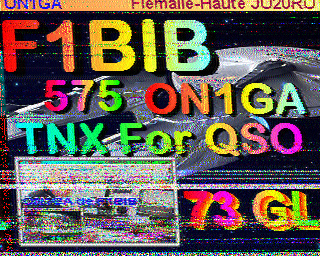
\includegraphics[width=0.85\textwidth]{foto/84}
    \caption{\scriptsize Bestätigung einer SSTV Verbindung an F1BIB von ON1GA mit dem RST 575 und zusätzlich dem ursprünglich empfangenen Bild}
    \label{e_digimode_ssb_sstv}
\end{figure}

   \end{column}
\end{columns}

\end{frame}

\begin{frame}
\frametitle{ATV}
\begin{itemize}
  \item \emph{Amateur Television} ist die Übertragung von Bewegtbildern
  \item Benötigt mehrere MHz Bandbreite (\qty{6}{\mega\hertz} und mehr)
  \item Deshalb nur ab \qty{70}{\centi\metre} Band aufwärts nutzbar
  \end{itemize}
\end{frame}

\begin{frame}
\only<1>{
\begin{QQuestion}{EE415}{Welcher Unterschied zwischen ATV und SSTV ist richtig?}{SSTV wird nur auf Kurzwelle, ATV auf UKW verwendet.}
{SSTV überträgt Standbilder, ATV bewegte Bilder.}
{SSTV belegt eine größere Bandbreite als ATV.}
{SSTV ist schwarzweiß, ATV in Farbe.}
\end{QQuestion}

}
\only<2>{
\begin{QQuestion}{EE415}{Welcher Unterschied zwischen ATV und SSTV ist richtig?}{SSTV wird nur auf Kurzwelle, ATV auf UKW verwendet.}
{\textbf{\textcolor{DARCgreen}{SSTV überträgt Standbilder, ATV bewegte Bilder.}}}
{SSTV belegt eine größere Bandbreite als ATV.}
{SSTV ist schwarzweiß, ATV in Farbe.}
\end{QQuestion}

}
\end{frame}%ENDCONTENT


\section{9600-Port}
\label{section:9600_port}
\begin{frame}%STARTCONTENT
\begin{itemize}
  \item Zur Umgehung von Filtern bieten manche FM-Funkgeräte einen separaten Port für Digimodes
  \item Dieser ist oft mit \emph{DATA} oder \emph{9600} beschriftet
  \item 9600 entsprechend der Datenrate in Baud, die damit übertragen werden kann
  \item Daran wird direkt das TNC (Terminal Node Controller) vom Computer angeschlossen
  \item Heute oft direkt als USB-Anschluss ausgeführt
  \end{itemize}
\end{frame}

\begin{frame}
\begin{columns}
    \begin{column}{0.48\textwidth}
    \begin{itemize}
  \item Sowohl Senden als auch Empfang findet ohne NF-Filter und NF-Endstufe statt
  \item Es wird direkt der FM-Modulator oder FM-Demodulator angesprochen
  \item Signale werden nicht verzerrt
  \end{itemize}

    \end{column}
   \begin{column}{0.48\textwidth}
       
\begin{figure}
    \DARCimage{0.85\linewidth}{354include}
    \caption{\scriptsize FM-Sender mit Zuführung des 9600-Baud-Datensignals an Punkt 2}
    \label{e_9600_port_fm_sender}
\end{figure}


\begin{figure}
    \DARCimage{0.85\linewidth}{355include}
    \caption{\scriptsize FM-Empfänger mit Abgreifen des 9600-Baud-Datensignals an Punkt 4}
    \label{e_9600_port_fm_empfaenger}
\end{figure}


   \end{column}
\end{columns}

\end{frame}

\begin{frame}
\begin{columns}
    \begin{column}{0.48\textwidth}
    \begin{itemize}
  \item Wurde früher für Packet Radio verwendet
  \item Heute für moderne und freie Modi wie M17
  \end{itemize}

    \end{column}
   \begin{column}{0.48\textwidth}
       
\begin{figure}
    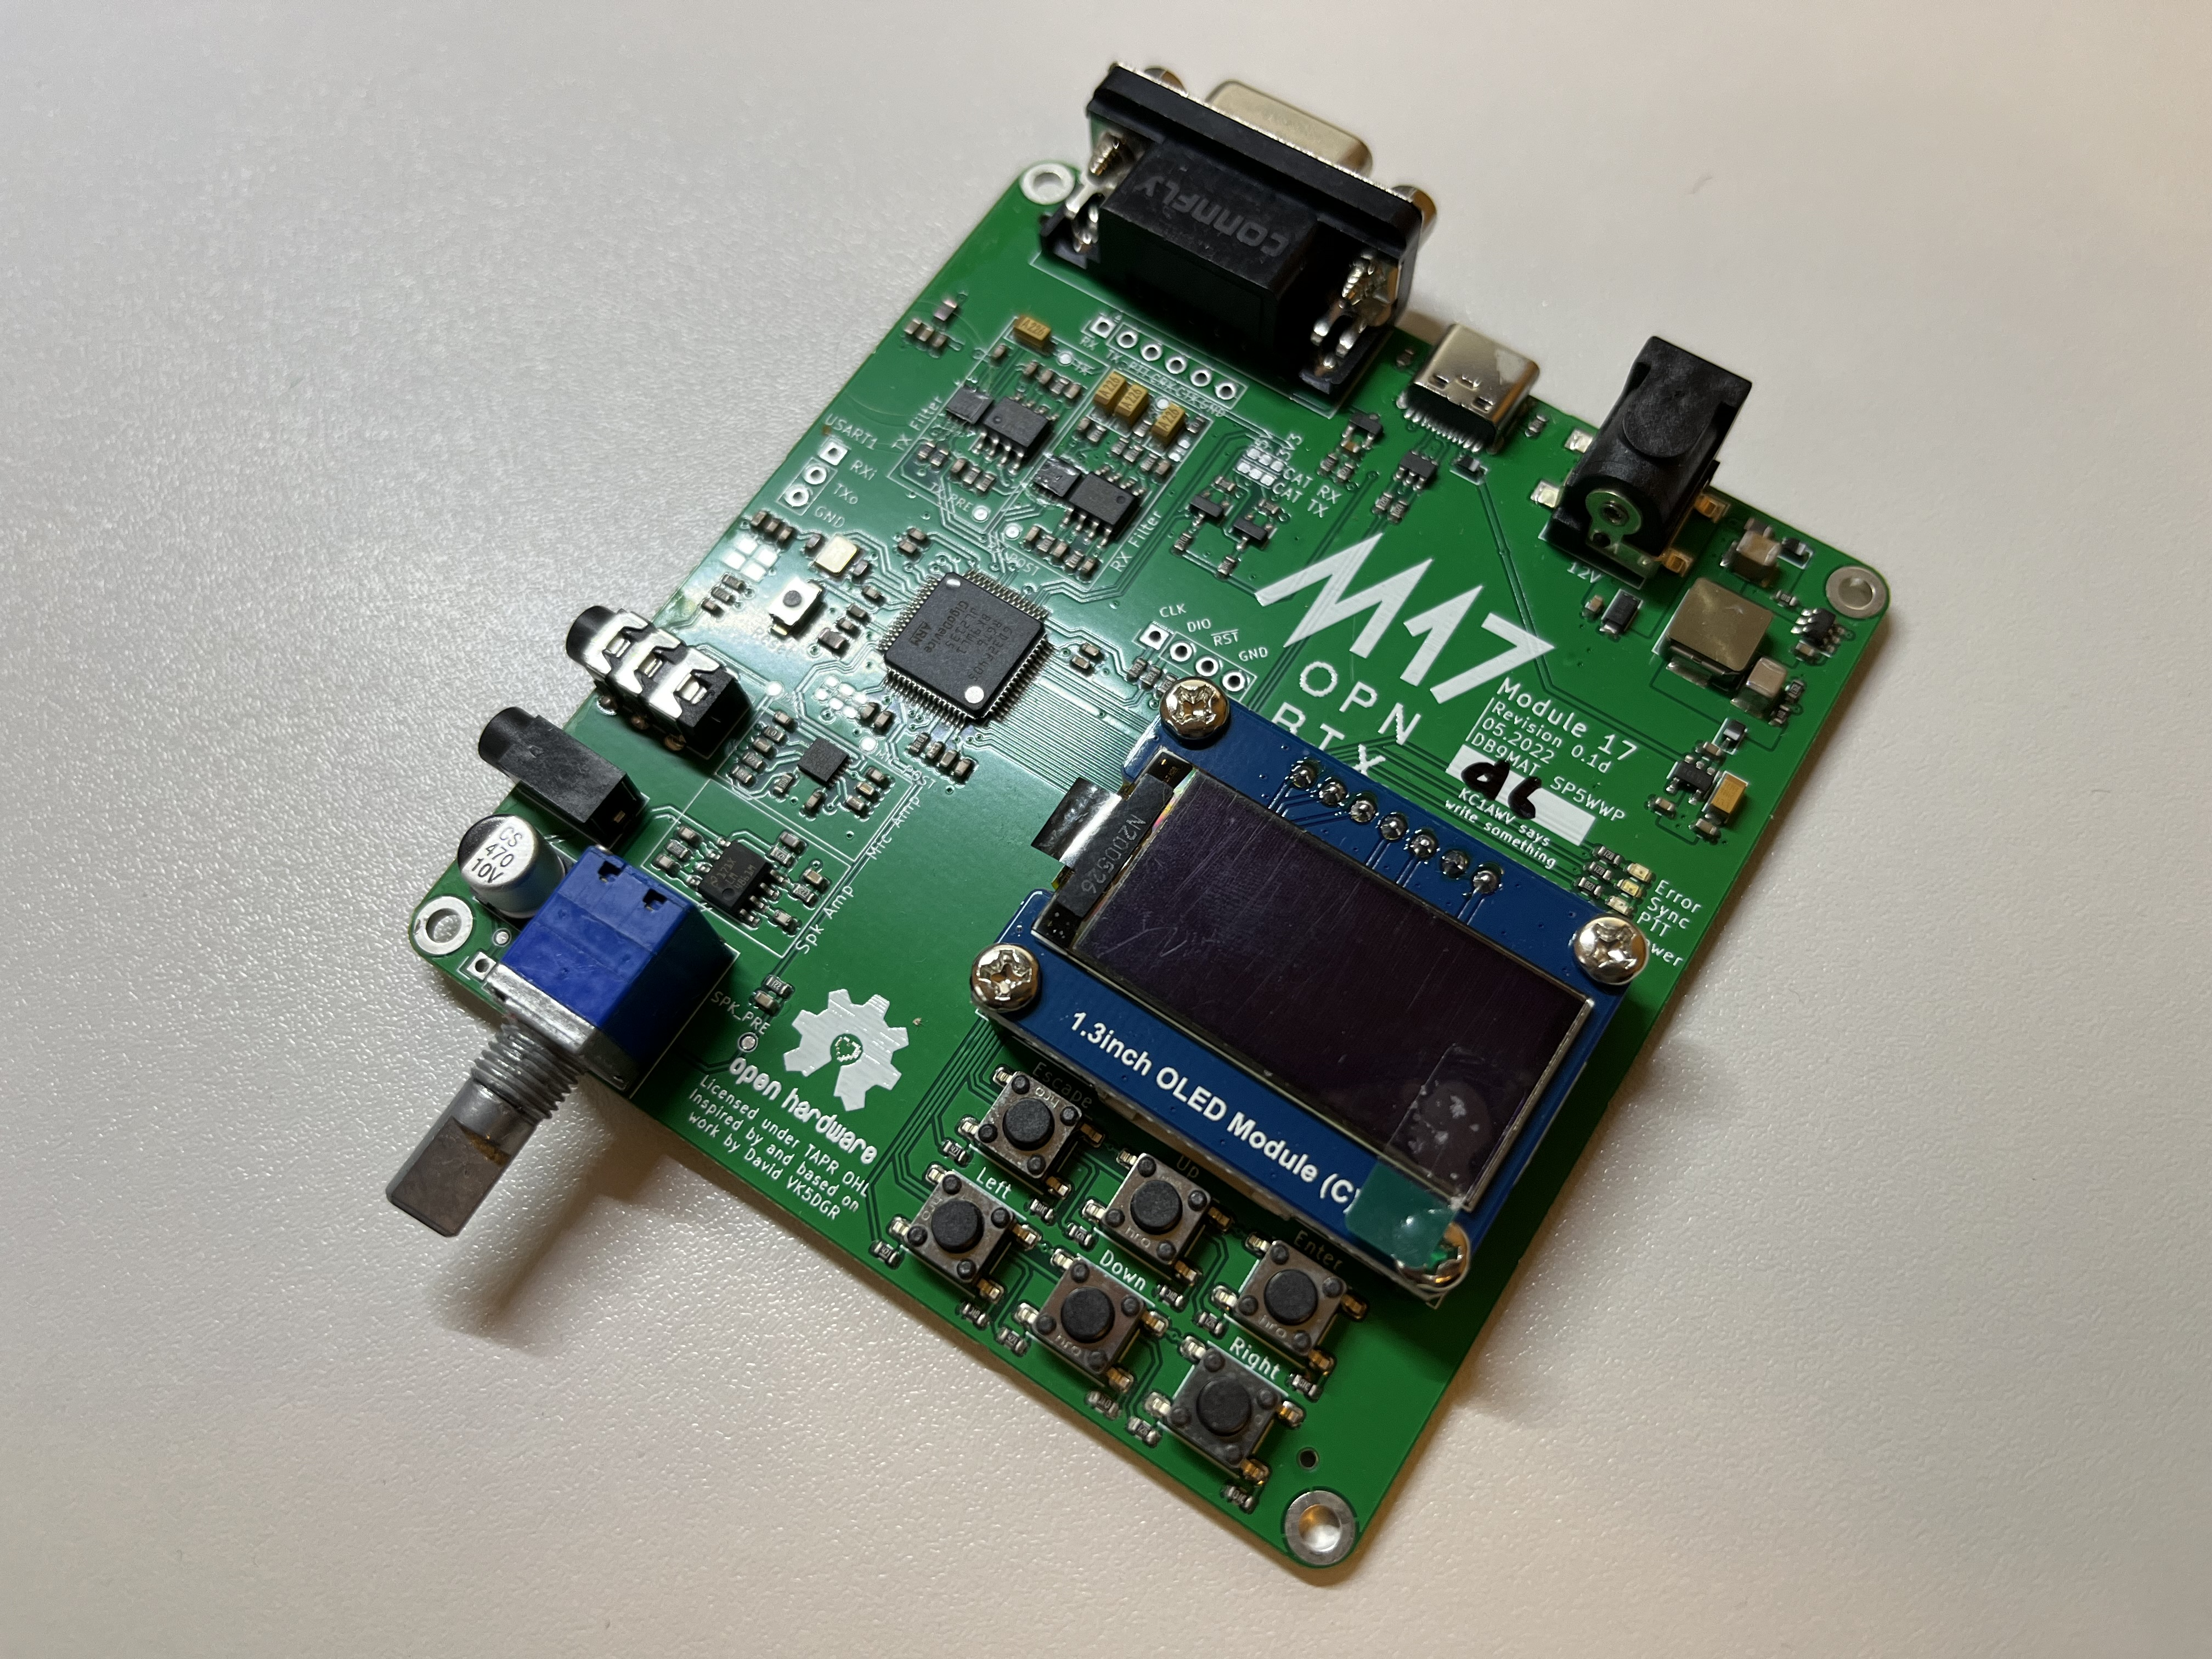
\includegraphics[width=0.85\textwidth]{foto/185}
    \caption{\scriptsize Module M17 ein TNC für das M17 Übertragungsverfahren}
    \label{m17_tnc}
\end{figure}

   \end{column}
\end{columns}

\end{frame}

\begin{frame}
\only<1>{
\begin{PQuestion}{EF309}{Welcher der eingezeichneten Punkte in einem FM-Sender ist für die Zuführung eines 9600-Baud-Datensignals am besten geeignet?}{Punkt 2}
{Punkt 1}
{Punkt 3}
{Punkt 4}
{\DARCimage{1.0\linewidth}{354include}}\end{PQuestion}

}
\only<2>{
\begin{PQuestion}{EF309}{Welcher der eingezeichneten Punkte in einem FM-Sender ist für die Zuführung eines 9600-Baud-Datensignals am besten geeignet?}{\textbf{\textcolor{DARCgreen}{Punkt 2}}}
{Punkt 1}
{Punkt 3}
{Punkt 4}
{\DARCimage{1.0\linewidth}{354include}}\end{PQuestion}

}
\end{frame}

\begin{frame}
\only<1>{
\begin{PQuestion}{EF219}{Manche FM-Transceiver verfügen über einen analogen Datenanschluss (z.~B. mit DATA beschriftet oder als 9600-Port bezeichnet). Welcher Punkt im dargestellten Empfangszweig wird über diesen Anschluss üblicherweise herausgeführt?}{Punkt 1}
{Punkt 4}
{Punkt 2}
{Punkt 3}
{\DARCimage{1.0\linewidth}{355include}}\end{PQuestion}

}
\only<2>{
\begin{PQuestion}{EF219}{Manche FM-Transceiver verfügen über einen analogen Datenanschluss (z.~B. mit DATA beschriftet oder als 9600-Port bezeichnet). Welcher Punkt im dargestellten Empfangszweig wird über diesen Anschluss üblicherweise herausgeführt?}{Punkt 1}
{\textbf{\textcolor{DARCgreen}{Punkt 4}}}
{Punkt 2}
{Punkt 3}
{\DARCimage{1.0\linewidth}{355include}}\end{PQuestion}

}
\end{frame}%ENDCONTENT


\section{Übersteuerung}
\label{section:digimod_uebersteuerung}
\begin{frame}%STARTCONTENT

\begin{columns}
    \begin{column}{0.48\textwidth}
    \begin{itemize}
  \item Zu starkes Audiosignal am Eingang eines Senders $\rightarrow$ Oberschwingungen
  \item Links ist in Gelb das erwünschte Signal
  \item Rechts davon die unerwünschten Oberschwingungen
  \end{itemize}

    \end{column}
   \begin{column}{0.48\textwidth}
       
\begin{figure}
    \DARCimage{0.85\linewidth}{720include}
    \caption{\scriptsize Ein übersteuertes FT8-Signal, ganz links das erwünschte, rechts davon die unerwünschten Oberschwingungen}
    \label{uebersteuerung_ft8}
\end{figure}


   \end{column}
\end{columns}

\end{frame}

\begin{frame}\begin{itemize}
  \item Zu Verzerrungen durch Übersteuerung kann es auch im Sendeverstärker kommen
  \item Um das zu verhindern, verfügen viele Funkgeräte über eine automatische Pegelregelung (englisch: Automatic Level Control, ALC) $\rightarrow$ regelt Verstärkung automatisch runter
  \item Bei digitalen Übertragungsverfahren kann die ALC jedoch Problemen führen
  \item Das Signal könnte je nach Lautstärke oder Frequenz die ALC zu verschiedenen Zeitpunkten unterschiedlich stark auslösen $\rightarrow$ Amplitude wird unerwünscht verändert
  \end{itemize}

\end{frame}

\begin{frame}\begin{itemize}
  \item ALC-Probleme hängen von verschiedenen Faktoren ab
  \item Übertragungsverfahren
  \item Umsetzung der ALC im Transceiver (Reaktions- und Haltezeit)
  \item Anzeige der ALC im Transceiver
  \item $\rightarrow$ greift die ALC nicht ein, erzeugt sie keine Probleme
  \end{itemize}
\end{frame}

\begin{frame}
\only<1>{
\begin{QQuestion}{EJ218}{Wie sollte bei digitalen Übertragungsverfahren (z. B. FT8, JS8, PSK31) der NF-Pegel am Eingang eines Funkgerätes mit automatischer Pegelregelung (ALC) im SSB-Betrieb eingestellt sein, um Störungen zu vermeiden?}{\qty{18}{\decibel} höher als die Lautstärke, bei der die automatische Pegelregelung (ALC) eingreift.}
{So niedrig, dass die automatische Pegelregelung (ALC) nicht eingreift.}
{Alle Bedienelemente sind auf das Maximum einzustellen.}
{Die NF-Lautstärke muss $-\infty$~dB (also Null) betragen.}
\end{QQuestion}

}
\only<2>{
\begin{QQuestion}{EJ218}{Wie sollte bei digitalen Übertragungsverfahren (z. B. FT8, JS8, PSK31) der NF-Pegel am Eingang eines Funkgerätes mit automatischer Pegelregelung (ALC) im SSB-Betrieb eingestellt sein, um Störungen zu vermeiden?}{\qty{18}{\decibel} höher als die Lautstärke, bei der die automatische Pegelregelung (ALC) eingreift.}
{\textbf{\textcolor{DARCgreen}{So niedrig, dass die automatische Pegelregelung (ALC) nicht eingreift.}}}
{Alle Bedienelemente sind auf das Maximum einzustellen.}
{Die NF-Lautstärke muss $-\infty$~dB (also Null) betragen.}
\end{QQuestion}

}
\end{frame}

\begin{frame}
\only<1>{
\begin{QQuestion}{EJ217}{Was kann auftreten, wenn bei digitalen Übertragungsverfahren (z. B. RTTY, FT8, Olivia) die automatische Pegelregelung (ALC) eines Funkgerätes im SSB-Betrieb eingreift?}{Störungen von Stationen auf anderen Frequenzbändern}
{Störungen von Computern oder anderen digitalen Geräten}
{Störungen von Übertragungen auf Nachbarfrequenzen}
{Störungen von nachfolgenden Sendungen auf derselben Frequenz}
\end{QQuestion}

}
\only<2>{
\begin{QQuestion}{EJ217}{Was kann auftreten, wenn bei digitalen Übertragungsverfahren (z. B. RTTY, FT8, Olivia) die automatische Pegelregelung (ALC) eines Funkgerätes im SSB-Betrieb eingreift?}{Störungen von Stationen auf anderen Frequenzbändern}
{Störungen von Computern oder anderen digitalen Geräten}
{\textbf{\textcolor{DARCgreen}{Störungen von Übertragungen auf Nachbarfrequenzen}}}
{Störungen von nachfolgenden Sendungen auf derselben Frequenz}
\end{QQuestion}

}
\end{frame}

\begin{frame}
\only<1>{
\begin{QQuestion}{EJ219}{Was ist zu tun, wenn es bei digitalen Übertragungsverfahren zu Störungen kommt, weil die automatische Pegelregelung (ALC) eines Funkgerätes im SSB-Betrieb eingreift?}{Die Sendeleistung sollte erhöht werden.}
{Der NF-Pegel am Eingang des Funkgerätes sollte reduziert werden.}
{Das Oberwellenfilter sollte abgeschaltet werden.}
{Es sollte mit der RIT gegengesteuert werden.}
\end{QQuestion}

}
\only<2>{
\begin{QQuestion}{EJ219}{Was ist zu tun, wenn es bei digitalen Übertragungsverfahren zu Störungen kommt, weil die automatische Pegelregelung (ALC) eines Funkgerätes im SSB-Betrieb eingreift?}{Die Sendeleistung sollte erhöht werden.}
{\textbf{\textcolor{DARCgreen}{Der NF-Pegel am Eingang des Funkgerätes sollte reduziert werden.}}}
{Das Oberwellenfilter sollte abgeschaltet werden.}
{Es sollte mit der RIT gegengesteuert werden.}
\end{QQuestion}

}
\end{frame}%ENDCONTENT


\section{Automatische Empfangsberichte}
\label{section:automatische_empfangsberichte}
\begin{frame}%STARTCONTENT
\begin{itemize}
  \item Mittels Digimodes empfangene Rufzeichen können an Plattformen geschickt werden
  \item Diese lassen sich auf einer Karte mit empfangenen Band darstellen
  \item Zum Testen der eigenen Ausbreitungsbedingungen
  \end{itemize}

\end{frame}

\begin{frame}
\frametitle{WSPR}
\begin{itemize}
  \item \emph{Weak Signal Progagation Reporter Network}
  \item QRP-Digimode, der rein zum Testen der eigenen Ausbreitungsbedingungen entwickelt wurde
  \item Es ist kein 2-Wege-QSO möglich
  \item Sehr langsame Übertragung mit hoher Fehlerkorrektur
  \item 1 Minute Senden, mehrere Minuten empfangen
  \item Ergebnisse werden an Server geschickt und lassen sich auf WSPRnet (\textcolor{DARCblue}{\faLink~\href{https://www.wsprnet.org/drupal/wsprnet/map}{www.wsprnet.org/drupal/wsprnet/map}}) darstellen
  \end{itemize}
\end{frame}

\begin{frame}
\only<1>{
\begin{QQuestion}{EE405}{Wie können Sie automatische Empfangsberichte zu Aussendungen erhalten, z.~B. um die Reichweite ihrer Sendeanlage zu testen?}{Durch Aussendung einer Nachricht mittels geeignetem digitalen Verfahren (z.~B. CW oder WSPR) und Suche nach Ihrem Rufzeichen auf passenden Internetplattformen}
{Durch Aussendung einer Nachricht mittels geeignetem digitalen Verfahren (z.~B. CW oder WSPR) unter Angabe Ihrer E-Mail-Adresse und der Anzahl der maximal gewünschten Empfangsberichte}
{Durch Aussendung Ihres Rufzeichens mittels Telegrafie (5~WPM) mit dem Zusatz \glqq AUTO RSVP\grqq{} (vom französischen \glqq répondez s'il vous pla\^it\grqq{}) und Abhören der \qty{10}{\kHz} höher gelegenen Frequenz}
{Durch Aussendung Ihres Rufzeichens mittels Telegrafie (12~WPM) mit dem Zusatz \glqq R\grqq{} (für Report) und Abhören der \qty{10}{\kHz} tiefer gelegenen Frequenz}
\end{QQuestion}

}
\only<2>{
\begin{QQuestion}{EE405}{Wie können Sie automatische Empfangsberichte zu Aussendungen erhalten, z.~B. um die Reichweite ihrer Sendeanlage zu testen?}{\textbf{\textcolor{DARCgreen}{Durch Aussendung einer Nachricht mittels geeignetem digitalen Verfahren (z.~B. CW oder WSPR) und Suche nach Ihrem Rufzeichen auf passenden Internetplattformen}}}
{Durch Aussendung einer Nachricht mittels geeignetem digitalen Verfahren (z.~B. CW oder WSPR) unter Angabe Ihrer E-Mail-Adresse und der Anzahl der maximal gewünschten Empfangsberichte}
{Durch Aussendung Ihres Rufzeichens mittels Telegrafie (5~WPM) mit dem Zusatz \glqq AUTO RSVP\grqq{} (vom französischen \glqq répondez s'il vous pla\^it\grqq{}) und Abhören der \qty{10}{\kHz} höher gelegenen Frequenz}
{Durch Aussendung Ihres Rufzeichens mittels Telegrafie (12~WPM) mit dem Zusatz \glqq R\grqq{} (für Report) und Abhören der \qty{10}{\kHz} tiefer gelegenen Frequenz}
\end{QQuestion}

}
\end{frame}%ENDCONTENT


\section{Paketvermittelte Netzwerke}
\label{section:paketvermittelte_netzwerke}
\begin{frame}%STARTCONTENT
\begin{itemize}
  \item Das HAMNET, das Netzwerk nur für Funkamateure, basiert auf dem Internet-Protokoll (IP).
  \item Deswegen kann man das Hamnet mit der gleichen Software, die auch für das Internet verwendet wird, nutzen.
  \item Im einfachsten Fall ist das ein Webbrowser.
  \end{itemize}
\end{frame}

\begin{frame}\begin{itemize}
  \item Das Internet-Protokoll (IP) weist den beteiligten Computern IP-Adressen zu, damit sie sich gegenseitig erreichen können.
  \item IP-Adressen werden als vier Dezimalzahlen mit einem Punkt dazwischen geschrieben. Beispiel: 141.17.5.18
  \item Jede Dezimalzahl hat eine Länge von 8 Bit, deswegen ist die größtmögliche Zahl 255 (binär: 11111111).
  \end{itemize}

\end{frame}

\begin{frame}\begin{itemize}
  \item IP-Adressen sind in einen Netz- und einen Hostanteil aufgeteilt.
  \item Bei allen Computern, die sich im selben Netzwerk befinden, ist der Anfang der IP-Adressen gleich, diesen Anfang nennt man Netzanteil.
  \item Der Netzanteil ist unterschiedlich groß, je nachdem wie viele Computer (Hosts) im Netzwerk verwaltet werden sollen.
  \end{itemize}
\end{frame}

\begin{frame}Beispiele:

\emph{10}.100.234.22 (kleiner Netzanteil, großer Hostanteil)

\emph{192.168.1}.252 (großer Netzanteil, kleiner Hostanteil)

Dieses Prinzip kennt man vom Telefonnetz. Die großen Städte haben kürzere Vorwahlen als kleine Städte.

\end{frame}

\begin{frame}
\begin{figure}
    \DARCimage{0.85\linewidth}{699include}
    \caption{\scriptsize IPv4-Adresse und Netzmaske in Dezimal- und Dualschreibweise}
    \label{netzmaske}
\end{figure}

\begin{itemize}
  \item Eine Subnetzmaske gibt die Aufteilung einer IP-Adresse in Netz- und Hostanteil an, indem sie alle Bits des Netzanteils als 1 darstellt.
  \end{itemize}
\end{frame}

\begin{frame}\begin{itemize}
  \item Es zwei Möglichkeiten dieses niederzuschreiben, Beispiel für einen Netzanteil von 24:
  \item 255.255.255.0, was binär 11111111.11111111.11111111.00000000 ist.
  \item Die Schreibweise mit dem Schrägstrich, zum Beispiel 192.168.111.90/24
  \end{itemize}

\end{frame}

\begin{frame}
\begin{figure}
    \DARCimage{0.85\linewidth}{706include}
    \caption{\scriptsize Ausschnitt aus einer Netzwerk-Infrastruktur}
    \label{netzwerk}
\end{figure}

\begin{itemize}
  \item Netzwerkgeräte können nur innerhalb ihres eigenen lokalen Netzwerks direkt miteinander kommunizieren.
  \end{itemize}
\end{frame}

\begin{frame}
\begin{figure}
    \DARCimage{0.85\linewidth}{706include}
    \caption{\scriptsize Ausschnitt aus einer Netzwerk-Infrastruktur}
    \label{netzwerk}
\end{figure}

\begin{itemize}
  \item Man erkennt sie daran, dass sich aus ihrer eigenen IP-Adresse und Subnetzmaske derselbe Netzanteil ergibt wie beim Partner.
  \end{itemize}
\end{frame}

\begin{frame}
\begin{figure}
    \DARCimage{0.85\linewidth}{706include}
    \caption{\scriptsize Ausschnitt aus einer Netzwerk-Infrastruktur}
    \label{netzwerk}
\end{figure}

\begin{itemize}
  \item In allen anderen Fällen schicken sie die Daten an einen Router. Das ist eine Zwischenstation, die zwei oder mehr Netzwerke miteinander verbindet, um die Datenpakete weiterzuleiten.
  \end{itemize}
\end{frame}

\begin{frame}
\only<1>{
\begin{QQuestion}{EE412}{Wie können Informationen innerhalb eines paketvermittelten Netzes zwischen zwei Stationen ausgetauscht werden, die sich nicht direkt erreichen können?}{Durch wiederholte Aussendung (Paketwiederholung)}
{Durch Weiterleitung über Zwischenstationen (Paketweiterleitung)}
{Durch Entpacken vor der Sendung (Paketdekompression)}
{Durch Zusammenfassung von Übertragungen (Paketdefragmentierung)}
\end{QQuestion}

}
\only<2>{
\begin{QQuestion}{EE412}{Wie können Informationen innerhalb eines paketvermittelten Netzes zwischen zwei Stationen ausgetauscht werden, die sich nicht direkt erreichen können?}{Durch wiederholte Aussendung (Paketwiederholung)}
{\textbf{\textcolor{DARCgreen}{Durch Weiterleitung über Zwischenstationen (Paketweiterleitung)}}}
{Durch Entpacken vor der Sendung (Paketdekompression)}
{Durch Zusammenfassung von Übertragungen (Paketdefragmentierung)}
\end{QQuestion}

}
\end{frame}

\begin{frame}
\only<1>{
\begin{QQuestion}{EE414}{Kann das Internetprotokoll (IP) im Amateurfunk verwendet werden?}{Nein, Internetnutzern würde so Zugang zum Amateurfunkband ermöglicht.}
{Ja, die Kodierung des Amateurfunkrufzeichens erfolgt in der Subnetzmaske.}
{Ja, es ist nicht auf das Internet beschränkt.}
{Nein, die benötigte Bandbreite steht im Amateurfunk nicht zur Verfügung.}
\end{QQuestion}

}
\only<2>{
\begin{QQuestion}{EE414}{Kann das Internetprotokoll (IP) im Amateurfunk verwendet werden?}{Nein, Internetnutzern würde so Zugang zum Amateurfunkband ermöglicht.}
{Ja, die Kodierung des Amateurfunkrufzeichens erfolgt in der Subnetzmaske.}
{\textbf{\textcolor{DARCgreen}{Ja, es ist nicht auf das Internet beschränkt.}}}
{Nein, die benötigte Bandbreite steht im Amateurfunk nicht zur Verfügung.}
\end{QQuestion}

}
\end{frame}

\begin{frame}
\only<1>{
\begin{QQuestion}{EE413}{Was ergibt sich aus der eingestellten IP-Adresse und Subnetzmaske einer Kommunikationsschnittstelle beim Internetprotokoll (IP)?}{Das Standardgateway und die maximale Anzahl der Zwischenstationen (Hops)}
{Die Protokoll- und Portnummer des über die Schnittstelle verwendeten Protokolls}
{Die Gegenstelle und die durch das Teilnetz verwendete Bandbreite}
{Der direkt (d.~h. ohne Router) über die Schnittstelle erreichbare Adressbereich}
\end{QQuestion}

}
\only<2>{
\begin{QQuestion}{EE413}{Was ergibt sich aus der eingestellten IP-Adresse und Subnetzmaske einer Kommunikationsschnittstelle beim Internetprotokoll (IP)?}{Das Standardgateway und die maximale Anzahl der Zwischenstationen (Hops)}
{Die Protokoll- und Portnummer des über die Schnittstelle verwendeten Protokolls}
{Die Gegenstelle und die durch das Teilnetz verwendete Bandbreite}
{\textbf{\textcolor{DARCgreen}{Der direkt (d.~h. ohne Router) über die Schnittstelle erreichbare Adressbereich}}}
\end{QQuestion}

}
\end{frame}%ENDCONTENT


\section{Amplituden- und Frequenzumtastung (ASK, FSK)}
\label{section:ask_fsk_afsk}
\begin{frame}%STARTCONTENT
\begin{itemize}
  \item Genauso wie es verschiedene analoge Modulationsverfahren gibt, gibt es auch verschiedene digitale Modulationsverfahren.
  \item Die grundlegenden Möglichkeiten ein Signal zu modulieren, also auf einen Hochfrequenzträger aufzuprägen, sind dieselben: Veränderung der Amplitude, der Frequenz oder der Phase des Trägers.
  \item Beim unmodulierten Träger hingegen bleiben Amplitude, Frequenz und Phasenlage konstant.
  \end{itemize}
\end{frame}

\begin{frame}\begin{itemize}
  \item Bei der Amplitudenumtastung (Amplitude Shift Keying, ASK) wird im einfachsten Fall zwischen zwei Amplituden gewechselt.
  \end{itemize}
    \pause
    
\begin{figure}
    \DARCimage{0.85\linewidth}{700include}
    \caption{\scriptsize Amplitudenumtastung (Amplitude-shift Keying)}
    \label{ask}
\end{figure}



\end{frame}

\begin{frame}\begin{itemize}
  \item Bei der Frequenzumstastung (Frequency Shift Keying, FSK) wechselt der Sender zwischen bestimmten Frequenzen.
  \end{itemize}
    \pause
    
\begin{figure}
    \DARCimage{0.85\linewidth}{703include}
    \caption{\scriptsize Frequenzumtastung (Frequency-shift Keying)}
    \label{fsk}
\end{figure}



\end{frame}

\begin{frame}\begin{itemize}
  \item Bei der Phasenumtastung (Phase Shift Keying, PSK) wechselt der Sender zwischen bestimmten Phasenlagen.
  \end{itemize}
    \pause
    
\begin{figure}
    \DARCimage{0.85\linewidth}{705include}
    \caption{\scriptsize Phasenumtastung (Phase-shift Keying)}
    \label{psk}
\end{figure}



\end{frame}

\begin{frame}
\only<1>{
\begin{question2x2}{EE406}{Welches der folgenden Diagramme zeigt einen erkennbar durch Amplitudenumtastung (ASK) modulierten Träger?}{\DARCimage{1.0\linewidth}{357include}}
{\DARCimage{1.0\linewidth}{356include}}
{\DARCimage{1.0\linewidth}{358include}}
{\DARCimage{1.0\linewidth}{359include}}
\end{question2x2}

}
\only<2>{
\begin{question2x2}{EE406}{Welches der folgenden Diagramme zeigt einen erkennbar durch Amplitudenumtastung (ASK) modulierten Träger?}{\DARCimage{1.0\linewidth}{357include}}
{\DARCimage{1.0\linewidth}{356include}}
{\textbf{\textcolor{DARCgreen}{\DARCimage{1.0\linewidth}{358include}}}}
{\DARCimage{1.0\linewidth}{359include}}
\end{question2x2}

}
\end{frame}

\begin{frame}
\only<1>{
\begin{question2x2}{EE407}{Welches der folgenden Diagramme zeigt einen erkennbar durch Frequenzumtastung (FSK) modulierten Träger?}{\DARCimage{1.0\linewidth}{357include}}
{\DARCimage{1.0\linewidth}{356include}}
{\DARCimage{1.0\linewidth}{358include}}
{\DARCimage{1.0\linewidth}{359include}}
\end{question2x2}

}
\only<2>{
\begin{question2x2}{EE407}{Welches der folgenden Diagramme zeigt einen erkennbar durch Frequenzumtastung (FSK) modulierten Träger?}{\textbf{\textcolor{DARCgreen}{\DARCimage{1.0\linewidth}{357include}}}}
{\DARCimage{1.0\linewidth}{356include}}
{\DARCimage{1.0\linewidth}{358include}}
{\DARCimage{1.0\linewidth}{359include}}
\end{question2x2}

}
\end{frame}

\begin{frame}
\only<1>{
\begin{question2x2}{AE401}{Welches der folgenden Diagramme zeigt einen erkennbar durch Phasenumtastung (PSK) modulierten Träger?}{\DARCimage{1.0\linewidth}{357include}}
{\DARCimage{1.0\linewidth}{356include}}
{\DARCimage{1.0\linewidth}{359include}}
{\DARCimage{1.0\linewidth}{358include}}
\end{question2x2}

}
\only<2>{
\begin{question2x2}{AE401}{Welches der folgenden Diagramme zeigt einen erkennbar durch Phasenumtastung (PSK) modulierten Träger?}{\DARCimage{1.0\linewidth}{357include}}
{\DARCimage{1.0\linewidth}{356include}}
{\textbf{\textcolor{DARCgreen}{\DARCimage{1.0\linewidth}{359include}}}}
{\DARCimage{1.0\linewidth}{358include}}
\end{question2x2}

}
\end{frame}

\begin{frame}
\only<1>{
\begin{question2x2}{EE101}{Welches der folgenden Diagramme zeigt einen unmodulierten Träger?}{\DARCimage{1.0\linewidth}{356include}}
{\DARCimage{1.0\linewidth}{357include}}
{\DARCimage{1.0\linewidth}{359include}}
{\DARCimage{1.0\linewidth}{358include}}
\end{question2x2}

}
\only<2>{
\begin{question2x2}{EE101}{Welches der folgenden Diagramme zeigt einen unmodulierten Träger?}{\textbf{\textcolor{DARCgreen}{\DARCimage{1.0\linewidth}{356include}}}}
{\DARCimage{1.0\linewidth}{357include}}
{\DARCimage{1.0\linewidth}{359include}}
{\DARCimage{1.0\linewidth}{358include}}
\end{question2x2}

}
\end{frame}%ENDCONTENT


\section{AFSK}
\label{section:afsk}
\begin{frame}%STARTCONTENT
\begin{itemize}
  \item Eine Sonderform der digitalen Modulation stellt das Audio Frequency Shift Keying (AFSK) dar.
  \item Im Gegensatz zu ASK steht hier das „A“ nicht für Amplitude, sondern für Audio, also für hörbare Frequenzen (Niederfrequenz).
  \item Es wird eine Frequenzumtastung (FSK) im Bereich deutlich unter 20 kHz durchgeführt. Oftmals wird der Bereich von ca. 300 Hz bis 2700 Hz genutzt.
  \item Für eine Aussendung per Funk muss eine weitere Modulation stattfinden, beispielsweise per FM, AM oder SSB.
  \end{itemize}

\end{frame}

\begin{frame}
\only<1>{
\begin{QQuestion}{EE408}{Was ist Audio Frequency Shift Keying (AFSK)?}{Ein unmodulierter Hochfrequenzträger, bei dem die Frequenzabweichung im hörbaren Bereich liegt
 }
{Ein hochfrequentes PSK-Signal, das mittels automatischer Umtastung auf zwei NF-Träger übertragen wird, um Bandbreite zu sparen}
{Eine Kombination aus digitaler Amplituden- und Frequenzmodulation, um zwei Informationen gleichzeitig zu übertragen}
{Ein durch Frequenzumtastung erzeugtes NF-Signal, mit dem ein Hochfrequenzträger (z.~B. mittels FM) moduliert werden kann}
\end{QQuestion}

}
\only<2>{
\begin{QQuestion}{EE408}{Was ist Audio Frequency Shift Keying (AFSK)?}{Ein unmodulierter Hochfrequenzträger, bei dem die Frequenzabweichung im hörbaren Bereich liegt
 }
{Ein hochfrequentes PSK-Signal, das mittels automatischer Umtastung auf zwei NF-Träger übertragen wird, um Bandbreite zu sparen}
{Eine Kombination aus digitaler Amplituden- und Frequenzmodulation, um zwei Informationen gleichzeitig zu übertragen}
{\textbf{\textcolor{DARCgreen}{Ein durch Frequenzumtastung erzeugtes NF-Signal, mit dem ein Hochfrequenzträger (z.~B. mittels FM) moduliert werden kann}}}
\end{QQuestion}

}
\end{frame}%ENDCONTENT


\section{Datenübertragungsrate}
\label{section:datenuebertragungsdrate}
\begin{frame}%STARTCONTENT
\begin{itemize}
  \item Die \emph{Bandbreite} ist der genutzte Frequenzbereich in \emph{Hz}
  \item Die \emph{Datenübertragungsrate} ist die je Zeiteinheit übertragene Datenmenge in \emph{Bit/s}
  \end{itemize}
\end{frame}

\begin{frame}\begin{itemize}
  \item In der Praxis erreichbare Datenübertragungsraten unterscheiden sich je nach Übertragungsverfahren und Funkbedingungen deutlich.
  \item WLAN und 5G unterstützen bei optimalen Bedingungen Datenübertragungsraten bis in den Bereich von Gigabit pro Sekunde.
  \item FT8 hingegen kann selbst unter widrigen Bedingungen eingesetzt werden, überträgt aber nur wenige Bit pro Sekunde.
  \end{itemize}
\end{frame}

\begin{frame}
\only<1>{
\begin{QQuestion}{EA106}{Welche Einheit wird üblicherweise für die Datenübertragungsrate verwendet?}{Dezibel (dB)}
{Baud (Bd)}
{Hertz (Hz)}
{Bit pro Sekunde (Bit/s)}
\end{QQuestion}

}
\only<2>{
\begin{QQuestion}{EA106}{Welche Einheit wird üblicherweise für die Datenübertragungsrate verwendet?}{Dezibel (dB)}
{Baud (Bd)}
{Hertz (Hz)}
{\textbf{\textcolor{DARCgreen}{Bit pro Sekunde (Bit/s)}}}
\end{QQuestion}

}
\end{frame}

\begin{frame}
\only<1>{
\begin{QQuestion}{EE401}{Welcher Unterschied besteht zwischen der Bandbreite und der Datenübertragungsrate?}{Als Bandbreite wird die übertragene Datenmenge (in Hz) und als Datenübertragungsrate die je Zeiteinheit übertragenen Symbole (in Baud) bezeichnet. }
{Als Bandbreite wird der genutzte Frequenzbereich (in Hz) und als Datenübertragungsrate die je Zeiteinheit übertragene Datenmenge (in Bit/s) bezeichnet.}
{Die Datenübertragungsrate (in Bit/s) entspricht der Symbolrate (in Baud). Die Bandbreite (in Hz) entspricht der maximal möglichen Datenübertragungsrate (in Bit/s).}
{Die Datenübertragungsrate (in Baud) entspricht der Symbolrate (in Bit/s). Die Bandbreite (in Hz) entspricht der minimal möglichen Datenübertragungsrate (in Baud).}
\end{QQuestion}

}
\only<2>{
\begin{QQuestion}{EE401}{Welcher Unterschied besteht zwischen der Bandbreite und der Datenübertragungsrate?}{Als Bandbreite wird die übertragene Datenmenge (in Hz) und als Datenübertragungsrate die je Zeiteinheit übertragenen Symbole (in Baud) bezeichnet. }
{\textbf{\textcolor{DARCgreen}{Als Bandbreite wird der genutzte Frequenzbereich (in Hz) und als Datenübertragungsrate die je Zeiteinheit übertragene Datenmenge (in Bit/s) bezeichnet.}}}
{Die Datenübertragungsrate (in Bit/s) entspricht der Symbolrate (in Baud). Die Bandbreite (in Hz) entspricht der maximal möglichen Datenübertragungsrate (in Bit/s).}
{Die Datenübertragungsrate (in Baud) entspricht der Symbolrate (in Bit/s). Die Bandbreite (in Hz) entspricht der minimal möglichen Datenübertragungsrate (in Baud).}
\end{QQuestion}

}
\end{frame}%ENDCONTENT


\section{Vielfachzugriff}
\label{section:vielfachzugriff}
\begin{frame}%STARTCONTENT

\frametitle{TDMA}
\begin{columns}
    \begin{column}{0.48\textwidth}
    \begin{itemize}
  \item Time Division Multiple Access – Zeitmultiplexverfahren
  \item Die digitalen Nutzdaten werden getrennt und nacheinander über die dieselbe Frequenz gesandt
  \item Am Empfänger wird der Datenstrom wieder zusammengesetzt
  \end{itemize}

    \end{column}
   \begin{column}{0.48\textwidth}
       
\begin{figure}
    \DARCimage{0.85\linewidth}{844include}
    \caption{\scriptsize Zeitmultiplexverfahren mit drei Signalen}
    \label{e_vielfachzugriff_tdma}
\end{figure}


   \end{column}
\end{columns}

\end{frame}

\begin{frame}
\only<1>{
\begin{QQuestion}{EE409}{Wie werden bei Zeitmultiplexverfahren (TDMA) mehrere Signale gleichzeitig übertragen?}{Im schnellen zeitlichen Wechsel auf derselben Frequenz}
{Zeitgleich auf unterschiedlichen Frequenzen}
{Zeitgleich mit Spreizcodierung im selben Frequenzbereich}
{Zeitgleich auf unterschiedlichen Wegen}
\end{QQuestion}

}
\only<2>{
\begin{QQuestion}{EE409}{Wie werden bei Zeitmultiplexverfahren (TDMA) mehrere Signale gleichzeitig übertragen?}{\textbf{\textcolor{DARCgreen}{Im schnellen zeitlichen Wechsel auf derselben Frequenz}}}
{Zeitgleich auf unterschiedlichen Frequenzen}
{Zeitgleich mit Spreizcodierung im selben Frequenzbereich}
{Zeitgleich auf unterschiedlichen Wegen}
\end{QQuestion}

}
\end{frame}

\begin{frame}
\frametitle{CDMA}
\begin{columns}
    \begin{column}{0.48\textwidth}
    \begin{itemize}
  \item Code Division Multiple Access – Codemultiplexverfahren
  \item Die digitalen Nutzdaten werden mit einem digitalen Code codiert (gemischt)
  \item Am Empfänger wird derselbe digitale Code zum decodieren verwendet
  \end{itemize}

    \end{column}
   \begin{column}{0.48\textwidth}
       
\begin{figure}
    \DARCimage{0.85\linewidth}{846include}
    \caption{\scriptsize Codemultiplexverfahren mit drei Signalen}
    \label{e_vielfachzugriff_cdma}
\end{figure}


   \end{column}
\end{columns}

\end{frame}

\begin{frame}
\only<1>{
\begin{QQuestion}{EE411}{Wie werden bei Codemultiplexverfahren (CDMA) mehrere Signale gleichzeitig übertragen?}{Im schnellen zeitlichen Wechsel auf derselben Frequenz}
{Zeitgleich auf unterschiedlichen Frequenzen}
{Zeitgleich mit Spreizcodierung im selben Frequenzbereich}
{Zeitgleich auf unterschiedlichen Wegen}
\end{QQuestion}

}
\only<2>{
\begin{QQuestion}{EE411}{Wie werden bei Codemultiplexverfahren (CDMA) mehrere Signale gleichzeitig übertragen?}{Im schnellen zeitlichen Wechsel auf derselben Frequenz}
{Zeitgleich auf unterschiedlichen Frequenzen}
{\textbf{\textcolor{DARCgreen}{Zeitgleich mit Spreizcodierung im selben Frequenzbereich}}}
{Zeitgleich auf unterschiedlichen Wegen}
\end{QQuestion}

}
\end{frame}

\begin{frame}
\frametitle{FDMA}
\begin{columns}
    \begin{column}{0.48\textwidth}
    \begin{itemize}
  \item Frequency Division Multiple Access – Frequenzmultiplexverfahren
  \item Das digitale Signal wird auf mehrere Frequenzen aufgeteilt
  \item Dadurch kann mehr Bandbreite verwendet werden
  \end{itemize}

    \end{column}
   \begin{column}{0.48\textwidth}
       
\begin{figure}
    \DARCimage{0.85\linewidth}{845include}
    \caption{\scriptsize Frequenzmultiplexverfahren mit drei Signalen}
    \label{e_vielfachzugriff_cdma}
\end{figure}


   \end{column}
\end{columns}

\end{frame}

\begin{frame}
\only<1>{
\begin{QQuestion}{EE410}{Wie werden bei Frequenzmultiplexverfahren (FDMA) mehrere Signale gleichzeitig übertragen?}{Zeitgleich auf unterschiedlichen Frequenzen}
{Im schnellen zeitlichen Wechsel auf derselben Frequenz}
{Zeitgleich mit Spreizcodierung im selben Frequenzbereich}
{Zeitgleich auf unterschiedlichen Wegen}
\end{QQuestion}

}
\only<2>{
\begin{QQuestion}{EE410}{Wie werden bei Frequenzmultiplexverfahren (FDMA) mehrere Signale gleichzeitig übertragen?}{\textbf{\textcolor{DARCgreen}{Zeitgleich auf unterschiedlichen Frequenzen}}}
{Im schnellen zeitlichen Wechsel auf derselben Frequenz}
{Zeitgleich mit Spreizcodierung im selben Frequenzbereich}
{Zeitgleich auf unterschiedlichen Wegen}
\end{QQuestion}

}
\end{frame}%ENDCONTENT


\title{DARC Amateurfunklehrgang Klasse E}
\author{Digitale Signalverarbeitung}
\institute{Deutscher Amateur Radio Club e.\,V.}
\begin{frame}
\maketitle
\end{frame}

\section{Digitale Signalverarbeitung}
\label{section:digitale_signalverarbeitung_einleitung}
\begin{frame}%STARTCONTENT
\begin{itemize}
  \item Im Bereich der Funktechnik spricht man bei Geräten, die mittels digitaler Signalverarbeitung arbeiten von sogenannten SDR-Geräten.
  \item \emph{SDR} steht dabei  für Software Defined Radio.
  \item In diesen Geräten ist zumindest ein Teil der Signalverarbeitung in Software realisiert.
  \item Dieses hat einen Kostenvorteil und bringt eine große Flexibilität mit sich.
  \end{itemize}
\end{frame}

\begin{frame}
\only<1>{
\begin{QQuestion}{EF603}{Worauf deutet die Bezeichnung SDR bei einem Transceiver oder Empfänger hin?}{Zumindest ein Teil der Signalaufbereitung ist in Software realisiert.}
{Es werden spezielle Antennenanschlüsse für digitale Signale verwendet.}
{Zumindest im NF-Bereich wird Analogtechnik eingesetzt, um besseren Klang zu erreichen.}
{Die Aussendung bzw. der Empfang erfolgt über das Internet und nicht per Funk.}
\end{QQuestion}

}
\only<2>{
\begin{QQuestion}{EF603}{Worauf deutet die Bezeichnung SDR bei einem Transceiver oder Empfänger hin?}{\textbf{\textcolor{DARCgreen}{Zumindest ein Teil der Signalaufbereitung ist in Software realisiert.}}}
{Es werden spezielle Antennenanschlüsse für digitale Signale verwendet.}
{Zumindest im NF-Bereich wird Analogtechnik eingesetzt, um besseren Klang zu erreichen.}
{Die Aussendung bzw. der Empfang erfolgt über das Internet und nicht per Funk.}
\end{QQuestion}

}
\end{frame}

\begin{frame}
\frametitle{A/D-Umsetzer}
\begin{itemize}
  \item Damit die Daten digital verarbeitet werden können, müssen sie zunächst digitalisiert werden.
  \item Dazu wird das analoge Signal mittels eines Analog-Digital Umsetzers (A/D-Umsetzer) in digitale Werte umgesetzt.
  \end{itemize}
\end{frame}

\begin{frame}
\begin{columns}
    \begin{column}{0.48\textwidth}
    \begin{itemize}
  \item Hierbei wird das analoge Signal in festen Zeitintervallen abgetastet und in einem digitalen Wertebereich (z.B. von -128 bis +127) abgebildet.
  \item Die einzelnen gemessenen Signalwerte werden als Samples (Proben) bezeichnet.
  \end{itemize}

    \end{column}
   \begin{column}{0.48\textwidth}
       
\begin{figure}
    \DARCimage{0.85\linewidth}{411include}
    \caption{\scriptsize Einfache Darstellung einer Sinuswelle aus 16 Samples und 7 Werten}
    \label{e_digitale_signalverarbeitung}
\end{figure}


   \end{column}
\end{columns}

\end{frame}

\begin{frame}
\only<1>{
\begin{QQuestion}{EF602}{Was ist die Voraussetzung, um ein analoges Signal mit digitaler Signalverarbeitung zu filtern? Das Eingangssignal muss zunächst~...}{von Oberschwingungen befreit werden.}
{demoduliert werden.}
{von Rauschen befreit werden.}
{digitalisiert werden.}
\end{QQuestion}

}
\only<2>{
\begin{QQuestion}{EF602}{Was ist die Voraussetzung, um ein analoges Signal mit digitaler Signalverarbeitung zu filtern? Das Eingangssignal muss zunächst~...}{von Oberschwingungen befreit werden.}
{demoduliert werden.}
{von Rauschen befreit werden.}
{\textbf{\textcolor{DARCgreen}{digitalisiert werden.}}}
\end{QQuestion}

}
\end{frame}

\begin{frame}
\frametitle{D/A-Umsetzer}
\begin{itemize}
  \item Nach der digitalen Verarbeitung des Signals wird es in einem Digital-Analog-Umsetzer (D/A-Umsetzer) wieder in ein analoges Signal verwandelt.
  \end{itemize}
\end{frame}

\begin{frame}
\only<1>{
\begin{PQuestion}{EF601}{Folgendes Blockschaltbild stellt das Prinzip einer digitalen Signalverarbeitung dar. Welche Aufgaben haben die beiden Blöcke 1 und 2?}{beides A/D-Umsetzer}
{1: D/A-Umsetzer, 2: A/D-Umsetzer}
{beides D/A-Umsetzer}
{1: A/D-Umsetzer, 2: D/A-Umsetzer}
{\DARCimage{1.0\linewidth}{96include}}\end{PQuestion}

}
\only<2>{
\begin{PQuestion}{EF601}{Folgendes Blockschaltbild stellt das Prinzip einer digitalen Signalverarbeitung dar. Welche Aufgaben haben die beiden Blöcke 1 und 2?}{beides A/D-Umsetzer}
{1: D/A-Umsetzer, 2: A/D-Umsetzer}
{beides D/A-Umsetzer}
{\textbf{\textcolor{DARCgreen}{1: A/D-Umsetzer, 2: D/A-Umsetzer}}}
{\DARCimage{1.0\linewidth}{96include}}\end{PQuestion}

}
\end{frame}%ENDCONTENT


\title{DARC Amateurfunklehrgang Klasse E}
\author{Antennen und Übertragungsleitungen}
\institute{Deutscher Amateur Radio Club e.\,V.}
\begin{frame}
\maketitle
\end{frame}

\section{Polarisation II}
\label{section:polarisation_2}
\begin{frame}%STARTCONTENT
\begin{itemize}
  \item Polarisation einer Antenne bezieht sich auf die Ausrichtung des elektrischen Feldes
  \item In Hauptstrahlrichtung
  \item In Bezug zur Erdoberfläche
  \item Die Polarisationsrichtung kann nicht immer an der Bauform der Antenne erkannt werden
  \end{itemize}

\end{frame}

\begin{frame}
\only<1>{
\begin{QQuestion}{EG222}{Die Polarisation einer Antenne~...}{wird nach der Ausrichtung der magnetischen Feldkomponente in der Hauptstrahlrichtung in Bezug zur Erdoberfläche angegeben.}
{wird nach der Ausrichtung der elektrischen Feldkomponente in der Hauptstrahlrichtung in Bezug zur Erdoberfläche angegeben.}
{entspricht der Richtung der magnetischen Feldkomponente des empfangenen oder ausgesendeten Feldes in Bezug auf die Nordrichtung (Azimut).}
{entspricht der Richtung der elektrischen Feldkomponente des empfangenen oder ausgesendeten Feldes in Bezug auf die Nordrichtung (Azimut).}
\end{QQuestion}

}
\only<2>{
\begin{QQuestion}{EG222}{Die Polarisation einer Antenne~...}{wird nach der Ausrichtung der magnetischen Feldkomponente in der Hauptstrahlrichtung in Bezug zur Erdoberfläche angegeben.}
{\textbf{\textcolor{DARCgreen}{wird nach der Ausrichtung der elektrischen Feldkomponente in der Hauptstrahlrichtung in Bezug zur Erdoberfläche angegeben.}}}
{entspricht der Richtung der magnetischen Feldkomponente des empfangenen oder ausgesendeten Feldes in Bezug auf die Nordrichtung (Azimut).}
{entspricht der Richtung der elektrischen Feldkomponente des empfangenen oder ausgesendeten Feldes in Bezug auf die Nordrichtung (Azimut).}
\end{QQuestion}

}
\end{frame}%ENDCONTENT


\section{Antennenformen II}
\label{section:antennenformen_2}
\begin{frame}%STARTCONTENT

\frametitle{Symmetrie}
\begin{itemize}
  \item Mittengespeiste Dipole sind \emph{symmetrische Antennen}
  \item Weist an beiden Polen (z.B. den Einspeisepunkten) bis auf das Vorzeichen die gleiche Spannung gegenüber Erde auf
  \item Bei Dipolen und darauf basierenden Yagi-Uda-Antennen der Fall
  \item Die Groundplane-Antenne ist \emph{unsymmetrisch}, da sie am Anschlusspunkt der Radiale Erdpotential hat
  \end{itemize}

\end{frame}

\begin{frame}
\only<1>{
\begin{QQuestion}{EG213}{Welche Antenne gehört \underline{nicht} zu den symmetrischen Antennen?}{mittengespeister $\lambda$/2-Dipol}
{Faltdipol}
{Lang-Yagi-Uda}
{Groundplane}
\end{QQuestion}

}
\only<2>{
\begin{QQuestion}{EG213}{Welche Antenne gehört \underline{nicht} zu den symmetrischen Antennen?}{mittengespeister $\lambda$/2-Dipol}
{Faltdipol}
{Lang-Yagi-Uda}
{\textbf{\textcolor{DARCgreen}{Groundplane}}}
\end{QQuestion}

}
\end{frame}

\begin{frame}
\frametitle{Schleifenantennen}
\begin{itemize}
  \item Draht von insgesamt etwa einer Wellenlänge
  \item In Form eines Kreises, Quadrats, Dreiecks, …
  \item Beliebt: Delta-Loop-Antenne in Form eines Delta (Δ), da nur ein Mast benötigt wird
  \end{itemize}
\end{frame}

\begin{frame}
\only<1>{
\begin{QQuestion}{EG101}{Wie nennt man eine Schleifenantenne, die aus drei gleich langen Drahtstücken besteht?}{3-Element-Beam}
{3-Element-Quad-Loop-Antenne}
{W3DZZ-Antenne}
{Delta-Loop-Antenne}
\end{QQuestion}

}
\only<2>{
\begin{QQuestion}{EG101}{Wie nennt man eine Schleifenantenne, die aus drei gleich langen Drahtstücken besteht?}{3-Element-Beam}
{3-Element-Quad-Loop-Antenne}
{W3DZZ-Antenne}
{\textbf{\textcolor{DARCgreen}{Delta-Loop-Antenne}}}
\end{QQuestion}

}
\end{frame}

\begin{frame}
\frametitle{Magnetic-Loop}
\begin{itemize}
  \item Magnetische Ringantenne, da Abstrahlung im Nahfeld über das Magnetfeld erfolgt
  \item Ca. $\frac{\lambda}{10}$ Umfang
  \item Wirkungsgrad bei \qty{1}{\percent}-\qty{10}{\percent} im Sendebetrieb
  \item Weniger Störungen bei elektrisch leitfähigen oder dämpfenden Gegenständen im Nahfeld
  \end{itemize}

\end{frame}

\begin{frame}
\only<1>{
\begin{QQuestion}{EG105}{Welche Antennenform eignet sich für Sendebetrieb und weist dabei im Nahfeld ein starkes magnetisches Feld auf?}{Eine Cubical-Quad-Antenne}
{Eine Ferritstabantenne}
{Ein Faltdipol}
{Eine magnetische Ringantenne mit einem Umfang von etwa $\lambda$/10}
\end{QQuestion}

}
\only<2>{
\begin{QQuestion}{EG105}{Welche Antennenform eignet sich für Sendebetrieb und weist dabei im Nahfeld ein starkes magnetisches Feld auf?}{Eine Cubical-Quad-Antenne}
{Eine Ferritstabantenne}
{Ein Faltdipol}
{\textbf{\textcolor{DARCgreen}{Eine magnetische Ringantenne mit einem Umfang von etwa $\lambda$/10}}}
\end{QQuestion}

}
\end{frame}

\begin{frame}
\frametitle{Endgespeiste Antennen}
\begin{itemize}
  \item Speisung vom Ende her
  \item Länge häufig $\frac{\lambda}{2}$
  \item Benötigt eine höhere Spannung
  \end{itemize}
\end{frame}

\begin{frame}
\frametitle{Fuchs-Antenne}
\begin{columns}
    \begin{column}{0.48\textwidth}
    \begin{itemize}
  \item Verwendung eines Anpassglieds (Transformator)
  \item Oft verwendet: Fuchskreis
  \end{itemize}

    \end{column}
   \begin{column}{0.48\textwidth}
       
\begin{figure}
    \DARCimage{0.85\linewidth}{310include}
    \caption{\scriptsize Schematische Darstellung einer Fuchs-Antenne mit Fuchskreis}
    \label{e_antennenformen_fuchskreis}
\end{figure}


   \end{column}
\end{columns}

\end{frame}

\begin{frame}
\only<1>{
\begin{PQuestion}{EG104}{Welche Antennenart ist hier dargestellt?  }{Dipol-Antenne}
{Windom-Antenne}
{Fuchs-Antenne}
{Groundplane-Antenne}
{\DARCimage{1.0\linewidth}{310include}}\end{PQuestion}

}
\only<2>{
\begin{PQuestion}{EG104}{Welche Antennenart ist hier dargestellt?  }{Dipol-Antenne}
{Windom-Antenne}
{\textbf{\textcolor{DARCgreen}{Fuchs-Antenne}}}
{Groundplane-Antenne}
{\DARCimage{1.0\linewidth}{310include}}\end{PQuestion}

}
\end{frame}

\begin{frame}
\only<1>{
\begin{PQuestion}{EG103}{Welche Antenne ist hier dargestellt?}{Einband-Drahtantenne mit Preselektor}
{Einseitig geerdeter Winkeldipol mit Oberwellenfilter}
{Endgespeiste Antenne mit Collins-Filter zur Anpassung}
{Endgespeiste Antenne mit einfachem Anpassglied}
{\DARCimage{1.0\linewidth}{310include}}\end{PQuestion}

}
\only<2>{
\begin{PQuestion}{EG103}{Welche Antenne ist hier dargestellt?}{Einband-Drahtantenne mit Preselektor}
{Einseitig geerdeter Winkeldipol mit Oberwellenfilter}
{Endgespeiste Antenne mit Collins-Filter zur Anpassung}
{\textbf{\textcolor{DARCgreen}{Endgespeiste Antenne mit einfachem Anpassglied}}}
{\DARCimage{1.0\linewidth}{310include}}\end{PQuestion}

}
\end{frame}

\begin{frame}
\frametitle{Richtwirkung}
\begin{itemize}
  \item Darstellung als \emph{Strahlungsdiagramm}
  \item Für eine Ebene wird in jede Richtung der Gewinn bzw. Feldstärke oder Strahlungsleistung aufgetragen
  \item Je weiter der Graphenverlauf vom Mittelpunkt entfernt ist, umso größer der Gewinn bzw. umso höher die Feldstärke und Strahlungsleistung im Fernfeld
  \item Oft wird Antenne mit darin dargestellt
  \end{itemize}
\end{frame}

\begin{frame}
\frametitle{Richtwirkung eines Dipols}
\begin{columns}
    \begin{column}{0.48\textwidth}
    \begin{itemize}
  \item Strahlt rechtwinklig vom Draht ab
  \item In einer Ebene betrachtet ergeben sich Keulen neben dem Dipol
  \item Ein vertikaler Dipol strahlt rund herum ab
  \end{itemize}

    \end{column}
   \begin{column}{0.48\textwidth}
       
\begin{figure}
    \DARCimage{0.85\linewidth}{261include}
    \caption{\scriptsize Strahlungsdiagramm eines Dipols}
    \label{e_antennenformen_strahlungsdiagramm_dipol}
\end{figure}


   \end{column}
\end{columns}

\end{frame}

\begin{frame}
\only<1>{
\begin{PQuestion}{EG215}{Für welche Antenne ist dieses Strahlungsdiagramm typisch?}{Yagi-Uda-Antenne}
{Halbwellendipol}
{Groundplane}
{Kugelstrahler}
{\DARCimage{0.5\linewidth}{261include}}\end{PQuestion}

}
\only<2>{
\begin{PQuestion}{EG215}{Für welche Antenne ist dieses Strahlungsdiagramm typisch?}{Yagi-Uda-Antenne}
{\textbf{\textcolor{DARCgreen}{Halbwellendipol}}}
{Groundplane}
{Kugelstrahler}
{\DARCimage{0.5\linewidth}{261include}}\end{PQuestion}

}
\end{frame}

\begin{frame}
\only<1>{
\begin{question2x2}{EG214}{Welches der Bilder zeigt das Strahlungsdiagramm eines Halbwellendipols?}{\DARCimage{1.0\linewidth}{450include}}
{\DARCimage{1.0\linewidth}{262include}}
{\DARCimage{1.0\linewidth}{268include}}
{\DARCimage{1.0\linewidth}{261include}}
\end{question2x2}

}
\only<2>{
\begin{question2x2}{EG214}{Welches der Bilder zeigt das Strahlungsdiagramm eines Halbwellendipols?}{\DARCimage{1.0\linewidth}{450include}}
{\DARCimage{1.0\linewidth}{262include}}
{\DARCimage{1.0\linewidth}{268include}}
{\textbf{\textcolor{DARCgreen}{\DARCimage{1.0\linewidth}{261include}}}}
\end{question2x2}

}
\end{frame}

\begin{frame}
\frametitle{Vertikaler Halbwellendipol}
\begin{itemize}
  \item Ein vertikal montierter Halbwellendipol hat eine flache Abstrahlung
  \item Beliebt im DX-Betrieb oder Kontakten über Direkt- oder Bodenwelle
  \end{itemize}
\end{frame}

\begin{frame}
\only<1>{
\begin{QQuestion}{EG219}{Eine $\lambda$/2-Vertikalantenne erzeugt~...}{elliptische Polarisation.}
{zirkulare Polarisation.}
{einen hohen Abstrahlwinkel.}
{einen flachen Abstrahlwinkel.}
\end{QQuestion}

}
\only<2>{
\begin{QQuestion}{EG219}{Eine $\lambda$/2-Vertikalantenne erzeugt~...}{elliptische Polarisation.}
{zirkulare Polarisation.}
{einen hohen Abstrahlwinkel.}
{\textbf{\textcolor{DARCgreen}{einen flachen Abstrahlwinkel.}}}
\end{QQuestion}

}
\end{frame}

\begin{frame}
\frametitle{5/8$\lambda$Antenne}
\begin{itemize}
  \item Gegen Erde oder Fahrzeugkarosserie erregte 5/8$\lambda$-Antenne
  \item Spezialfall einer Vertikalantenne
  \item Die Länge ist so gewählt, damit sich ein optimaler Gewinn ergibt
  \end{itemize}
\end{frame}

\begin{frame}
\only<1>{
\begin{QQuestion}{EG108}{Warum ist eine 5/8-$\lambda$-Antenne besser als eine $\lambda$/4-Antenne für VHF-UHF-Mobilbetrieb geeignet? Sie~...}{ist weniger störanfällig.}
{verträgt mehr Leistung.}
{ist leichter zu montieren.}
{hat mehr Gewinn.}
\end{QQuestion}

}
\only<2>{
\begin{QQuestion}{EG108}{Warum ist eine 5/8-$\lambda$-Antenne besser als eine $\lambda$/4-Antenne für VHF-UHF-Mobilbetrieb geeignet? Sie~...}{ist weniger störanfällig.}
{verträgt mehr Leistung.}
{ist leichter zu montieren.}
{\textbf{\textcolor{DARCgreen}{hat mehr Gewinn.}}}
\end{QQuestion}

}
\end{frame}

\begin{frame}
\frametitle{Groundplane-Antenne}
\begin{columns}
    \begin{column}{0.48\textwidth}
    \begin{itemize}
  \item Strahlt rechtwinklig zum Strahler ab
  \item Strahlungsdiagramm wird von oben betrachtet
  \item Nahezu ein Rundstrahler, bis auf den Bereich der Radiale
  \end{itemize}

    \end{column}
   \begin{column}{0.48\textwidth}
       
\begin{figure}
    \DARCimage{0.85\linewidth}{268include}
    \caption{\scriptsize Strahlungsdiagramm einer Groundplane-Antenne von oben betrachtet}
    \label{e_antennenformen_strahlungsdiagramm_groundplane}
\end{figure}


   \end{column}
\end{columns}

\end{frame}

\begin{frame}
\only<1>{
\begin{PQuestion}{EG216}{Für welche Antenne ist dieses Strahlungsdiagramm typisch?}{Yagi-Uda}
{Kugelstrahler}
{Dipol}
{Groundplane}
{\DARCimage{0.5\linewidth}{268include}}\end{PQuestion}

}
\only<2>{
\begin{PQuestion}{EG216}{Für welche Antenne ist dieses Strahlungsdiagramm typisch?}{Yagi-Uda}
{Kugelstrahler}
{Dipol}
{\textbf{\textcolor{DARCgreen}{Groundplane}}}
{\DARCimage{0.5\linewidth}{268include}}\end{PQuestion}

}
\end{frame}

\begin{frame}
\frametitle{Richtantenne}
\begin{columns}
    \begin{column}{0.48\textwidth}
    \begin{itemize}
  \item Gewinn ist in eine Richtung deutlich höher als in andere Richtungen
  \end{itemize}

    \end{column}
   \begin{column}{0.48\textwidth}
       
\begin{figure}
    \DARCimage{0.85\linewidth}{262include}
    \caption{\scriptsize Strahlungsdiagramm einer Richtantenne}
    \label{e_antennenformen_strahlungsdiagramm_richtantenne}
\end{figure}


   \end{column}
\end{columns}

\end{frame}

\begin{frame}
\only<1>{
\begin{PQuestion}{EG217}{Dieses Strahlungsdiagramm ist typisch für~...}{einen Viertelwellenstrahler.}
{einen Halbwellendipol.}
{eine Richtantenne.}
{eine Marconi-Antenne.}
{\DARCimage{0.5\linewidth}{262include}}\end{PQuestion}

}
\only<2>{
\begin{PQuestion}{EG217}{Dieses Strahlungsdiagramm ist typisch für~...}{einen Viertelwellenstrahler.}
{einen Halbwellendipol.}
{\textbf{\textcolor{DARCgreen}{eine Richtantenne.}}}
{eine Marconi-Antenne.}
{\DARCimage{0.5\linewidth}{262include}}\end{PQuestion}

}
\end{frame}

\begin{frame}
\frametitle{Antennen für UHF/VHF/SHF}
\begin{columns}
    \begin{column}{0.48\textwidth}
    \begin{itemize}
  \item Nur für hohe Frequenzen geeignet
  \item Im Kurzwellenbereich unüblich, da sie unhandliche Größen erreichen würden
  \end{itemize}

    \end{column}
   \begin{column}{0.48\textwidth}
       \begin{itemize}
  \item Hornstrahler
  \item Parabolantennen
  \item Patchantennen auf Leiterplatten
  \item Sperrtopfantenne
  \end{itemize}

   \end{column}
\end{columns}

\end{frame}

\begin{frame}
\frametitle{Weitere Antennen für Kurzwelle}
\begin{itemize}
  \item Die \emph{Windom-Antenne} ist eine Mehrbandantenne, die aufgrund zwei unterschiedlich langer Schenkel eine Anpassung für mehrere Frequenzen erlaubt
  \item Die \emph{W3DZZ-Antenne} ist ein Dipol für 40m und 80m, deren Enden sich durch Sperrkreise bei 40m verkürzen
  \end{itemize}
\end{frame}

\begin{frame}
\only<1>{
\begin{QQuestion}{EG106}{Was sind gebräuchliche Kurzwellen-Amateurfunksendeantennen?}{Schlitzantenne, Groundplane-Antenne, Hornstrahler, Dipol-Antenne, Windom-Antenne}
{Langdraht-Antenne, Groundplane-Antenne, Parabolantenne, Windom-Antenne, Delta-Loop-Antenne}
{Groundplane-Antenne, Dipol-Antenne, Windom-Antenne, Delta-Loop-Antenne, Patchantenne}
{Langdraht-Antenne, Yagi-Uda-Antenne, Dipol-Antenne, Windom-Antenne, Delta-Loop-Antenne}
\end{QQuestion}

}
\only<2>{
\begin{QQuestion}{EG106}{Was sind gebräuchliche Kurzwellen-Amateurfunksendeantennen?}{Schlitzantenne, Groundplane-Antenne, Hornstrahler, Dipol-Antenne, Windom-Antenne}
{Langdraht-Antenne, Groundplane-Antenne, Parabolantenne, Windom-Antenne, Delta-Loop-Antenne}
{Groundplane-Antenne, Dipol-Antenne, Windom-Antenne, Delta-Loop-Antenne, Patchantenne}
{\textbf{\textcolor{DARCgreen}{Langdraht-Antenne, Yagi-Uda-Antenne, Dipol-Antenne, Windom-Antenne, Delta-Loop-Antenne}}}
\end{QQuestion}

}
\end{frame}

\begin{frame}
\only<1>{
\begin{QQuestion}{EG107}{Sie wollen verschiedene Antennen für den Funkbetrieb auf Kurzwelle für das \qty{80}{\m}-Band testen. Welche drei Antennen sind besonders geeignet?  }{Kreuz-Yagi-Uda, Groundplane-Antenne, Dipol}
{Dipol, Delta-Loop, W3DZZ-Antenne}
{Dipol, Sperrtopfantenne, W3DZZ-Antenne}
{Dipol, Delta-Loop, Parabolspiegel}
\end{QQuestion}

}
\only<2>{
\begin{QQuestion}{EG107}{Sie wollen verschiedene Antennen für den Funkbetrieb auf Kurzwelle für das \qty{80}{\m}-Band testen. Welche drei Antennen sind besonders geeignet?  }{Kreuz-Yagi-Uda, Groundplane-Antenne, Dipol}
{\textbf{\textcolor{DARCgreen}{Dipol, Delta-Loop, W3DZZ-Antenne}}}
{Dipol, Sperrtopfantenne, W3DZZ-Antenne}
{Dipol, Delta-Loop, Parabolspiegel}
\end{QQuestion}

}
\end{frame}%ENDCONTENT


\section{Antennenlänge und -resonanz}
\label{section:antenne_laenge_resonanz}
\begin{frame}%STARTCONTENT
\begin{itemize}
  \item Die Drähte einer Antennen können eine beliebige Länge oder Form haben
  \item Jedoch ist dann deren Wellenwiderstand anders
  \item Dieser Wellenwiderstand muss an die Speiseleitung angepasst werden, z.B. durch einen Balun
  \end{itemize}
\end{frame}

\begin{frame}
\only<1>{
\begin{QQuestion}{EG102}{Eine Drahtantenne für den Amateurfunk im KW-Bereich~...}{kann grundsätzlich eine beliebige Länge haben.}
{muss unbedingt $\lambda/2$ lang sein.}
{muss genau $\lambda/4$ lang sein.}
{muss eine Länge von $3/4~\lambda$  haben.}
\end{QQuestion}

}
\only<2>{
\begin{QQuestion}{EG102}{Eine Drahtantenne für den Amateurfunk im KW-Bereich~...}{\textbf{\textcolor{DARCgreen}{kann grundsätzlich eine beliebige Länge haben.}}}
{muss unbedingt $\lambda/2$ lang sein.}
{muss genau $\lambda/4$ lang sein.}
{muss eine Länge von $3/4~\lambda$  haben.}
\end{QQuestion}

}
\end{frame}

\begin{frame}
\only<1>{
\begin{QQuestion}{EG109}{Berechnen Sie die elektrische Länge eines 5/8 $\lambda$ langen Vertikalstrahlers für das \qty{10}{\m}-Band (\qty{28,5}{\MHz}).}{\qty{2,08}{\m}}
{\qty{3,29}{\m}}
{\qty{6,58}{\m}}
{\qty{5,26}{\m}}
\end{QQuestion}

}
\only<2>{
\begin{QQuestion}{EG109}{Berechnen Sie die elektrische Länge eines 5/8 $\lambda$ langen Vertikalstrahlers für das \qty{10}{\m}-Band (\qty{28,5}{\MHz}).}{\qty{2,08}{\m}}
{\qty{3,29}{\m}}
{\textbf{\textcolor{DARCgreen}{\qty{6,58}{\m}}}}
{\qty{5,26}{\m}}
\end{QQuestion}

}
\end{frame}

\begin{frame}
\frametitle{Lösungsweg}
Anstatt direkt die ungefähre Wellenlänge des 10m-Bands zu verwenden, wird hier erst die angegebene Frequenz in die exakte Wellenlänge umgerechnet.

\begin{equation} \begin{split} l &= \frac{5}{8}\lambda\\ &= \frac{5}{8} \cdot \dfrac{300}{28,5MHz}\\ &= \frac{5}{8} \cdot 10,53m\\ &= 6,58m\\ \end{split} \end{equation}

\end{frame}

\begin{frame}
\frametitle{Faltdipol}
\begin{columns}
    \begin{column}{0.48\textwidth}
    \begin{itemize}
  \item Ein Draht einer Wellenlänge wird an den Enden zur Länge eines Halbwellen-Dipols umgebogen
  \item Die Einspeisung ist immer noch in der Mitte
  \end{itemize}

    \end{column}
   \begin{column}{0.48\textwidth}
       
\begin{figure}
    \DARCimage{0.85\linewidth}{531include}
    \caption{\scriptsize Die Elemente einer Yagi-Uda-Antenne mit einem Faltdipol als Strahler bei der Nummer 2}
    \label{e_antenne_laenge_resonanz}
\end{figure}


   \end{column}
\end{columns}

\end{frame}

\begin{frame}
\only<1>{
\begin{QQuestion}{EG110}{Die Länge des Drahtes zur Herstellung eines Faltdipols entspricht~...}{einer Wellenlänge.}
{einer Halbwellenlänge.}
{zwei Wellenlängen.}
{vier Wellenlängen.}
\end{QQuestion}

}
\only<2>{
\begin{QQuestion}{EG110}{Die Länge des Drahtes zur Herstellung eines Faltdipols entspricht~...}{\textbf{\textcolor{DARCgreen}{einer Wellenlänge.}}}
{einer Halbwellenlänge.}
{zwei Wellenlängen.}
{vier Wellenlängen.}
\end{QQuestion}

}
\end{frame}%ENDCONTENT


\section{Verkürzungsfaktor I}
\label{section:verkuerzungsfaktor_1}
\begin{frame}%STARTCONTENT

\begin{columns}
    \begin{column}{0.48\textwidth}
    Wellenausbreitung in Luft und Vakuum:

$\lambda = \dfrac{c}{f}$


    \end{column}
   \begin{column}{0.48\textwidth}
       \begin{itemize}
  \item Leitungen und Antennendrähte benötigen einen Korrekturfaktor
  \item Den \emph{Verkürzungsfaktor} $k_\mathrm{v}$
  \item In etwa \qty{95}{\percent} zur Vakuumausbreitung
  \item $\lambda_\mathrm{Leitung} = k_\mathrm{v} \cdot \dfrac{c}{f}$
  \end{itemize}

   \end{column}
\end{columns}

\end{frame}

\begin{frame}
\only<1>{
\begin{QQuestion}{EG201}{Der Verkürzungsfaktor ist~...}{das Verhältnis des Leiterwiderstandes zum Fußpunktwiderstand der Antenne.}
{das Verhältnis von Durchmesser zur Länge eines Leiters.}
{das Verhältnis der Ausbreitungsgeschwindigkeit entlang einer Leitung zur Ausbreitungsgeschwindigkeit im Vakuum.}
{die Wurzel aus dem Verhältnis von Induktivität zur Kapazität einer Leitung.}
\end{QQuestion}

}
\only<2>{
\begin{QQuestion}{EG201}{Der Verkürzungsfaktor ist~...}{das Verhältnis des Leiterwiderstandes zum Fußpunktwiderstand der Antenne.}
{das Verhältnis von Durchmesser zur Länge eines Leiters.}
{\textbf{\textcolor{DARCgreen}{das Verhältnis der Ausbreitungsgeschwindigkeit entlang einer Leitung zur Ausbreitungsgeschwindigkeit im Vakuum.}}}
{die Wurzel aus dem Verhältnis von Induktivität zur Kapazität einer Leitung.}
\end{QQuestion}

}
\end{frame}

\begin{frame}\begin{itemize}
  \item Korrekturfaktor hängt von Drahtdurchmesser, Isolierung und Umgebungseinflüssen ab
  \item Bei Drahtantennen sind diese für Resonanz um ca. \qty{5}{\percent} zu kürzen
  \end{itemize}
\end{frame}

\begin{frame}
\only<1>{
\begin{QQuestion}{EG202}{Welcher Prozentsatz entspricht dem Verkürzungsfaktor (Korrekturfaktor), der üblicherweise für die Berechnung der Länge einer Drahtantenne verwendet wird?}{\qty{75}{\percent}}
{\qty{95}{\percent}}
{\qty{66}{\percent}}
{\qty{100}{\percent}}
\end{QQuestion}

}
\only<2>{
\begin{QQuestion}{EG202}{Welcher Prozentsatz entspricht dem Verkürzungsfaktor (Korrekturfaktor), der üblicherweise für die Berechnung der Länge einer Drahtantenne verwendet wird?}{\qty{75}{\percent}}
{\textbf{\textcolor{DARCgreen}{\qty{95}{\percent}}}}
{\qty{66}{\percent}}
{\qty{100}{\percent}}
\end{QQuestion}

}
\end{frame}%ENDCONTENT


\section{Fußpunktimpedanz I}
\label{section:fusspunktimpedanz_1}
\begin{frame}%STARTCONTENT

\frametitle{Mittengespeister Dipol}
\begin{itemize}
  \item Speiseimpedanz 73,1 Ω
  \item Im Freiraum, also bei einer Aufbauhöhe von min. einer Wellenlänge
  \item Recht nahe bei 50 Ω
  \end{itemize}
\end{frame}

\begin{frame}
\only<1>{
\begin{QQuestion}{EG207}{Die Fußpunktimpedanz eines mittengespeisten Halbwellendipols in einer Höhe von mindestens einer Wellenlänge über dem Boden beträgt ungefähr~...}{\qty{50}{\ohm}.}
{\qty{75}{\ohm}.}
{\qty{30}{\ohm}.}
{\qty{600}{\ohm}.}
\end{QQuestion}

}
\only<2>{
\begin{QQuestion}{EG207}{Die Fußpunktimpedanz eines mittengespeisten Halbwellendipols in einer Höhe von mindestens einer Wellenlänge über dem Boden beträgt ungefähr~...}{\qty{50}{\ohm}.}
{\textbf{\textcolor{DARCgreen}{\qty{75}{\ohm}.}}}
{\qty{30}{\ohm}.}
{\qty{600}{\ohm}.}
\end{QQuestion}

}
\end{frame}

\begin{frame}
\frametitle{Mittengespeister Dipol}
\begin{itemize}
  \item Bei geringerer Aufbauhöhe kommt es zu Wechselwirkungen mit dem Boden
  \item Speiseimpedanz ca. 40 Ω bis 90 Ω
  \end{itemize}
\end{frame}

\begin{frame}
\only<1>{
\begin{QQuestion}{EG208}{Der Fußpunktwiderstand in der Mitte eines Halbwellendipols beträgt je nach Aufbauhöhe ungefähr~...}{\qtyrange{100}{120}{\ohm}.}
{\qtyrange{40}{90}{\ohm}.}
{\qtyrange{120}{240}{\ohm}.}
{\qtyrange{240}{600}{\ohm}.}
\end{QQuestion}

}
\only<2>{
\begin{QQuestion}{EG208}{Der Fußpunktwiderstand in der Mitte eines Halbwellendipols beträgt je nach Aufbauhöhe ungefähr~...}{\qtyrange{100}{120}{\ohm}.}
{\textbf{\textcolor{DARCgreen}{\qtyrange{40}{90}{\ohm}.}}}
{\qtyrange{120}{240}{\ohm}.}
{\qtyrange{240}{600}{\ohm}.}
\end{QQuestion}

}
\end{frame}

\begin{frame}
\only<1>{
\begin{QQuestion}{EG209}{Welchen Eingangswiderstand hat ein gestreckter mittengespeister Halbwellendipol?}{ca. \num{40} bis \qty{90}{\ohm}}
{ca. \qty{30}{\ohm}}
{ca. \qty{120}{\ohm}}
{ca. \num{240} bis \qty{300}{\ohm}}
\end{QQuestion}

}
\only<2>{
\begin{QQuestion}{EG209}{Welchen Eingangswiderstand hat ein gestreckter mittengespeister Halbwellendipol?}{\textbf{\textcolor{DARCgreen}{ca. \num{40} bis \qty{90}{\ohm}}}}
{ca. \qty{30}{\ohm}}
{ca. \qty{120}{\ohm}}
{ca. \num{240} bis \qty{300}{\ohm}}
\end{QQuestion}

}
\end{frame}

\begin{frame}
\frametitle{Faltdipol}
\begin{itemize}
  \item Antennenabschnitte sind teilweise parallel geführt
  \item Verdoppelt die Spannung
  \item Halbiert den Strom
  \item $R = \frac{2 \cdot U}{\frac{I}{2}} = 4 \cdot \frac{U}{I}$
  \item Speiseimpedanz vervierfacht sich: ca. 240 Ω bis 300 Ω
  \end{itemize}

\end{frame}

\begin{frame}
\only<1>{
\begin{QQuestion}{EG210}{Welchen Eingangs- bzw. Fußpunktwiderstand hat ein Faltdipol?}{ca. \qtyrange{240}{300}{\ohm}}
{ca. \qtyrange{30}{60}{\ohm}}
{ca. \qty{60}{\ohm}}
{ca. \qty{120}{\ohm}}
\end{QQuestion}

}
\only<2>{
\begin{QQuestion}{EG210}{Welchen Eingangs- bzw. Fußpunktwiderstand hat ein Faltdipol?}{\textbf{\textcolor{DARCgreen}{ca. \qtyrange{240}{300}{\ohm}}}}
{ca. \qtyrange{30}{60}{\ohm}}
{ca. \qty{60}{\ohm}}
{ca. \qty{120}{\ohm}}
\end{QQuestion}

}
\end{frame}

\begin{frame}
\frametitle{Groundplane-Antenne}
\begin{itemize}
  \item Ein Dipolschenkel entfällt und wird durch eine Erde mit möglichst geringem Widerstand ersetzt
  \item Hälfte eines Dipols im Freiraum
  \item $\rightarrow$ Speisewiderstand: $\dfrac{73,1 Ω}{2} \approx 37 Ω$
  \item Radiale um \qty{45}{\degree} nach unten abwinkeln ergibt zusätzliche Abstrahlung
  \item $\rightarrow$ Speisewiderstand: 50 Ω
  \end{itemize}
\end{frame}

\begin{frame}
\only<1>{
\begin{QQuestion}{EG211}{Welchen Eingangswiderstand hat eine Groundplane-Antenne?}{ca. \qty{600}{\ohm}}
{ca. \qtyrange{60}{120}{\ohm}}
{ca. \qtyrange{30}{50}{\ohm}}
{ca. \qty{240}{\ohm}}
\end{QQuestion}

}
\only<2>{
\begin{QQuestion}{EG211}{Welchen Eingangswiderstand hat eine Groundplane-Antenne?}{ca. \qty{600}{\ohm}}
{ca. \qtyrange{60}{120}{\ohm}}
{\textbf{\textcolor{DARCgreen}{ca. \qtyrange{30}{50}{\ohm}}}}
{ca. \qty{240}{\ohm}}
\end{QQuestion}

}
\end{frame}%ENDCONTENT


\section{Yagi-Uda Antenne II}
\label{section:yagi_uda_2}
\begin{frame}%STARTCONTENT

\frametitle{Funktionsprinzip}
\begin{columns}
    \begin{column}{0.48\textwidth}
    \begin{itemize}
  \item Einspeisung an \emph{Strahler} ausgeführt als Dipol oder Faltdipol
  \item Welle trifft auf längeren \emph{Reflektor} und kürzeren \emph{Direktor}
  \item Es kann auch mehrere Direktoren geben
  \end{itemize}

    \end{column}
   \begin{column}{0.48\textwidth}
       
\begin{figure}
    \DARCimage{0.85\linewidth}{531include}
    \caption{\scriptsize Die Elemente einer Yagi-Uda-Antenne}
    \label{e_yagi_uda_aufbau}
\end{figure}


   \end{column}
\end{columns}

\end{frame}

\begin{frame}
\only<1>{
\begin{PQuestion}{EG111}{Das folgende Bild enthält eine einfache Richtantenne. Die Bezeichnungen der Elemente in numerischer Reihenfolge lauten~...}{1 Strahler, 2 Direktor und 3 Reflektor.}
{1 Reflektor, 2 Strahler und 3 Direktor.}
{1 Direktor, 2 Strahler und 3 Reflektor.}
{1 Direktor, 2 Reflektor und 3 Strahler.}
{\DARCimage{1.0\linewidth}{531include}}\end{PQuestion}

}
\only<2>{
\begin{PQuestion}{EG111}{Das folgende Bild enthält eine einfache Richtantenne. Die Bezeichnungen der Elemente in numerischer Reihenfolge lauten~...}{1 Strahler, 2 Direktor und 3 Reflektor.}
{\textbf{\textcolor{DARCgreen}{1 Reflektor, 2 Strahler und 3 Direktor.}}}
{1 Direktor, 2 Strahler und 3 Reflektor.}
{1 Direktor, 2 Reflektor und 3 Strahler.}
{\DARCimage{1.0\linewidth}{531include}}\end{PQuestion}

}
\end{frame}

\begin{frame}
\frametitle{Parasitäre Elemente}
\begin{itemize}
  \item Reflektor und Direktor schwingen ohne elektrische Verbindung zum Strahler zu haben
  \item Haben auch keine Antenneneinspeisung
  \item Nehmen dennoch Energie auf und geben sie wieder ab
  \end{itemize}
\end{frame}

\begin{frame}
\only<1>{
\begin{QQuestion}{EG212}{An welchem Element einer Yagi-Uda-Antenne erfolgt die Energieeinspeisung? Sie erfolgt am~...}{Direktor}
{Strahler}
{Reflektor}
{Strahler und am Reflektor gleichzeitig}
\end{QQuestion}

}
\only<2>{
\begin{QQuestion}{EG212}{An welchem Element einer Yagi-Uda-Antenne erfolgt die Energieeinspeisung? Sie erfolgt am~...}{Direktor}
{\textbf{\textcolor{DARCgreen}{Strahler}}}
{Reflektor}
{Strahler und am Reflektor gleichzeitig}
\end{QQuestion}

}
\end{frame}

\begin{frame}
\frametitle{Richtwirkung}
\begin{columns}
    \begin{column}{0.48\textwidth}
    \begin{itemize}
  \item Zwischen Strahler und Elementen gibt es eine räumliche und zeitliche Phasenverschiebung
  \item Durch die Überlagerung der Abstrahlung entsteht eine Richtwirkung
  \item \emph{Destruktive Interferenz}: Wellen löschen sich aus
  \item \emph{Konstruktive Interferenz}: Wellen verstärken sich
  \end{itemize}

    \end{column}
   \begin{column}{0.48\textwidth}
       
   \end{column}
\end{columns}

\end{frame}

\begin{frame}
\frametitle{Strahlungsdiagramm}
\begin{columns}
    \begin{column}{0.48\textwidth}
    \begin{itemize}
  \item Große Hauptkeule in Richtung der Direktoren
  \item Kleine Nebenkeulen und insbesondere Rückkeule
  \end{itemize}

    \end{column}
   \begin{column}{0.48\textwidth}
       
\begin{figure}
    \DARCimage{0.85\linewidth}{265include}
    \caption{\scriptsize Strahlungsdiagramm einer Yagi-Uda-Antenne}
    \label{e_yagi_uda_strahlungsdiagramm}
\end{figure}


   \end{column}
\end{columns}

\end{frame}

\begin{frame}
\only<1>{
\begin{PQuestion}{EG218}{Für welche Antenne ist dieses Strahlungsdiagramm typisch?}{Yagi-Uda}
{Groundplane}
{Dipol}
{Kugelstrahler}
{\DARCimage{1.0\linewidth}{265include}}\end{PQuestion}

}
\only<2>{
\begin{PQuestion}{EG218}{Für welche Antenne ist dieses Strahlungsdiagramm typisch?}{\textbf{\textcolor{DARCgreen}{Yagi-Uda}}}
{Groundplane}
{Dipol}
{Kugelstrahler}
{\DARCimage{1.0\linewidth}{265include}}\end{PQuestion}

}
\end{frame}%ENDCONTENT


\section{Parabolspiegel I}
\label{section:parabolspiegel_1}
\begin{frame}%STARTCONTENT

\frametitle{Mikrowellen}
\begin{itemize}
  \item Frequenzen zwischen \qty{1}{\giga\hertz} und \qty{300}{\giga\hertz}
  \item Wellenlänge von Millimetern bis wenigen Dezimetern
  \item Können von Metallen reflektiert werden 
  \end{itemize}

\end{frame}

\begin{frame}
\frametitle{Parabolspiegel}
\begin{columns}
    \begin{column}{0.48\textwidth}
    \begin{itemize}
  \item Parabolisch geformte Metalloberfläche oder engmaschiges Gitter
  \item Parallel einfallende Wellen werden auf einem Punkt vor dem Spiegel gebündelt
  \end{itemize}

    \end{column}
   \begin{column}{0.48\textwidth}
       
\begin{figure}
    \DARCimage{0.85\linewidth}{850include}
    \caption{\scriptsize Funktionsweise eines Parabolspiegels}
    \label{e_parabolspiegel_funktion}
\end{figure}


   \end{column}
\end{columns}

\end{frame}

\begin{frame}
\only<1>{
\begin{QQuestion}{EG113}{Eine scharf bündelnde Antenne für den Mikrowellenbereich besteht häufig aus einem~...}{paraboloid geformten Spiegelkörper und einer Erregerantenne (Feed).}
{paraboloid geformten Spiegelkörper und einem isotropen Strahler.}
{zylindrisch konvex geformten Spiegelkörper und einer Erregerantenne (Feed).}
{hyperbolisch konkav geformten Spiegelkörper und einem isotropen Strahler.}
\end{QQuestion}

}
\only<2>{
\begin{QQuestion}{EG113}{Eine scharf bündelnde Antenne für den Mikrowellenbereich besteht häufig aus einem~...}{\textbf{\textcolor{DARCgreen}{paraboloid geformten Spiegelkörper und einer Erregerantenne (Feed).}}}
{paraboloid geformten Spiegelkörper und einem isotropen Strahler.}
{zylindrisch konvex geformten Spiegelkörper und einer Erregerantenne (Feed).}
{hyperbolisch konkav geformten Spiegelkörper und einem isotropen Strahler.}
\end{QQuestion}

}
\end{frame}

\begin{frame}
\frametitle{Beugungseffekt}
\begin{itemize}
  \item Durch die Welleneigenschaften kommt es zu Beugungseffekten
  \item Bündelung kommt nicht genau in einem Punkt zustande
  \item Abweichung kann durch Größe der Schüssel kompensiert werden
  \item Gewinn wird dadurch erhöht
  \item Optimal: Einige Wellenlängen oder mehr
  \end{itemize}
\end{frame}

\begin{frame}
\only<1>{
\begin{QQuestion}{EG114}{Welcher Durchmesser sollte für eine Parabolspiegelantenne im Hinblick auf möglichst hohen Gewinn gewählt werden?}{Höchstens drei Wellenlängen (Lambda) der verwendeten Frequenz.}
{Genau zwei Wellenlängen (Lambda) der verwendeten Frequenz.}
{Mindestens fünf Wellenlängen (Lambda) der verwendeten Frequenz.}
{Eine Wellenlänge (Lambda) der verwendeten Frequenz.}
\end{QQuestion}

}
\only<2>{
\begin{QQuestion}{EG114}{Welcher Durchmesser sollte für eine Parabolspiegelantenne im Hinblick auf möglichst hohen Gewinn gewählt werden?}{Höchstens drei Wellenlängen (Lambda) der verwendeten Frequenz.}
{Genau zwei Wellenlängen (Lambda) der verwendeten Frequenz.}
{\textbf{\textcolor{DARCgreen}{Mindestens fünf Wellenlängen (Lambda) der verwendeten Frequenz.}}}
{Eine Wellenlänge (Lambda) der verwendeten Frequenz.}
\end{QQuestion}

}
\end{frame}%ENDCONTENT


\section{Strom- und Spannungsspeisung I}
\label{section:strom_spannung_speisung_1}
\begin{frame}%STARTCONTENT

\frametitle{Speisewiderstand}
\begin{itemize}
  \item Eine Antenne wird mit Spannung und Strom gespeist
  \item Deren Verhältnis zueinander ergibt den Speisewiderstand
  \item Für Leistung müssen immer Spannung \underline{und} Strom vorhanden sein
  \item Wäre eines von beiden 0, erfolgt keine Leistungsabgabe
  \item Speisewiderstand hängt vom Ort der Einspeisung ab
  \end{itemize}

\end{frame}

\begin{frame}
\frametitle{Stromgespeiste Antennen}
\begin{itemize}
  \item Hoher Strom bei vergleichsweise geringer Spannung am Speisepunkt
  \item Niedriger Speisewiderstand
  \item ca. 36 Ω bis 100 Ω
  \item Niederohmiges Verhalten
  \end{itemize}
\end{frame}

\begin{frame}
\frametitle{Spannungsgespeiste Antenne}
\begin{itemize}
  \item Hohe Spannung bei vergleichsweise geringem Strom am Speisepunkt
  \item Hoher Speisewiderstand
  \item ca. 1500 Ω bis 4000 Ω
  \item Hochohmiges Verhalten
  \end{itemize}
\end{frame}

\begin{frame}
\frametitle{Einspeisung am Halbwellendipol}
\begin{itemize}
  \item Ladungsträger schwingen hin und her
  \item In der Mitte werden besonders viele Ladungsträger bewegt $\rightarrow$ Strombauch
  \item An den Enden entstehen besonders hohe Spannungen $\rightarrow$ Spannungsbauch
  \item Wenige Ladungsträger $\rightarrow$ Stromknoten
  \item Keine Spannung $\rightarrow$ Spannungsknoten
  \end{itemize}

\end{frame}

\begin{frame}
\begin{columns}
    \begin{column}{0.48\textwidth}
    \begin{itemize}
  \item Strombauch in der Mitte
  \item Spannungsbauch an den Enden
  \item Stromknoten an den Enden
  \item Spannungsknoten in der Mitte
  \end{itemize}

    \end{column}
   \begin{column}{0.48\textwidth}
       
\begin{figure}
    \DARCimage{0.85\linewidth}{787include}
    \caption{\scriptsize Halbwellendipol mit Spannungs- und Stromverteilung}
    \label{e_strom_spannung_speisung_dipol}
\end{figure}


   \end{column}
\end{columns}

\end{frame}

\begin{frame}
\only<1>{
\begin{QQuestion}{EG203}{Welche Aussage zur Strom- und Spannungsverteilung auf einem Dipol ist richtig?}{Am Einspeisepunkt eines Dipols entsteht immer ein Spannungsknoten und ein Strombauch.}
{An den Enden eines Dipols entsteht immer ein Spannungsknoten und ein Strombauch.}
{An den Enden eines Dipols entsteht immer ein Stromknoten und ein Spannungsbauch.}
{Am Einspeisepunkt eines Dipols entsteht immer ein Spannungsbauch und ein Stromknoten.}
\end{QQuestion}

}
\only<2>{
\begin{QQuestion}{EG203}{Welche Aussage zur Strom- und Spannungsverteilung auf einem Dipol ist richtig?}{Am Einspeisepunkt eines Dipols entsteht immer ein Spannungsknoten und ein Strombauch.}
{An den Enden eines Dipols entsteht immer ein Spannungsknoten und ein Strombauch.}
{\textbf{\textcolor{DARCgreen}{An den Enden eines Dipols entsteht immer ein Stromknoten und ein Spannungsbauch.}}}
{Am Einspeisepunkt eines Dipols entsteht immer ein Spannungsbauch und ein Stromknoten.}
\end{QQuestion}

}
\end{frame}

\begin{frame}
\only<1>{
\begin{QQuestion}{EG204}{Ein Dipol wird stromgespeist, wenn an seinem Einspeisepunkt~...}{ein Spannungsbauch und ein Stromknoten vorhanden sind. Er ist dann hochohmig.}
{ein Spannungsknoten und ein Strombauch vorhanden sind. Er ist dann niederohmig.}
{ein Spannungs- und ein Strombauch vorhanden sind. Er ist dann niederohmig.}
{ein Spannungs- und ein Stromknoten vorhanden sind. Er ist dann hochohmig.}
\end{QQuestion}

}
\only<2>{
\begin{QQuestion}{EG204}{Ein Dipol wird stromgespeist, wenn an seinem Einspeisepunkt~...}{ein Spannungsbauch und ein Stromknoten vorhanden sind. Er ist dann hochohmig.}
{\textbf{\textcolor{DARCgreen}{ein Spannungsknoten und ein Strombauch vorhanden sind. Er ist dann niederohmig.}}}
{ein Spannungs- und ein Strombauch vorhanden sind. Er ist dann niederohmig.}
{ein Spannungs- und ein Stromknoten vorhanden sind. Er ist dann hochohmig.}
\end{QQuestion}

}
\end{frame}

\begin{frame}
\only<1>{
\begin{QQuestion}{EG206}{Ein Halbwellendipol wird auf der Grundfrequenz in der Mitte~...}{spannungsgespeist.}
{stromgespeist.}
{endgespeist.}
{parallel gespeist.}
\end{QQuestion}

}
\only<2>{
\begin{QQuestion}{EG206}{Ein Halbwellendipol wird auf der Grundfrequenz in der Mitte~...}{spannungsgespeist.}
{\textbf{\textcolor{DARCgreen}{stromgespeist.}}}
{endgespeist.}
{parallel gespeist.}
\end{QQuestion}

}
\end{frame}

\begin{frame}
\frametitle{Endgespeister Halbwellendipol}
\begin{itemize}
  \item Spannungsgespeiste Antenne
  \item Hoher Speisewiderstand
  \end{itemize}
\end{frame}

\begin{frame}
\only<1>{
\begin{QQuestion}{EG205}{Ein Dipol wird spannungsgespeist, wenn an seinem Einspeisepunkt~...}{ein Spannungsknoten und ein Strombauch liegt. Er ist dann niederohmig.}
{ein Spannungsbauch und ein Stromknoten liegt. Er ist dann hochohmig.}
{ein Spannungs- und ein Strombauch liegt. Er ist dann niederohmig.}
{ein Spannungs- und ein Stromknoten liegt. Er ist dann hochohmig.}
\end{QQuestion}

}
\only<2>{
\begin{QQuestion}{EG205}{Ein Dipol wird spannungsgespeist, wenn an seinem Einspeisepunkt~...}{ein Spannungsknoten und ein Strombauch liegt. Er ist dann niederohmig.}
{\textbf{\textcolor{DARCgreen}{ein Spannungsbauch und ein Stromknoten liegt. Er ist dann hochohmig.}}}
{ein Spannungs- und ein Strombauch liegt. Er ist dann niederohmig.}
{ein Spannungs- und ein Stromknoten liegt. Er ist dann hochohmig.}
\end{QQuestion}

}
\end{frame}%ENDCONTENT


\section{Bauch und Knoten von Strom und Spannung}
\label{section:bauch_knoten}
\begin{frame}%STARTCONTENT
\end{frame}%ENDCONTENT


\section{Antennengewinn in dBi und dBd}
\label{section:antennengewinn}
\begin{frame}%STARTCONTENT

\frametitle{Richtwirkung}
\begin{itemize}
  \item \emph{Isotropstrahler}: Hypothetische Antenne, die in alle Richtungen gleich stark abstrahlt
  \item Eine reale Antenne weist eine Richtwirkung auf
  \item In bestimmten Richtungen stärker als der Isotropstrahler
  \item In bestimmten Richtungen schwächer als der Isotropstrahler
  \item Die \emph{Hauptstrahlrichtung} ist die Richtung mit dem maximalen Antennengewinn
  \end{itemize}
\end{frame}

\begin{frame}
\frametitle{Gewinn in dBi}
\begin{itemize}
  \item Gewinn in eine Richtung gegenüber dem Isotropstrahler
  \item Kann in dB angegeben werden
  \item Bei Bezug auf den Isotropstrahler wird \emph{dBi} verwendet
  \end{itemize}
\end{frame}

\begin{frame}
\only<1>{
\begin{QQuestion}{EG220}{Der Gewinn von Antennen wird häufig in dBi angegeben. Auf welche Vergleichsantenne bezieht man sich dabei? Man bezieht sich dabei auf den~...}{Halbwellenstrahler.}
{Isotropstrahler.}
{Horizontalstrahler.}
{Vertikalstrahler.}
\end{QQuestion}

}
\only<2>{
\begin{QQuestion}{EG220}{Der Gewinn von Antennen wird häufig in dBi angegeben. Auf welche Vergleichsantenne bezieht man sich dabei? Man bezieht sich dabei auf den~...}{Halbwellenstrahler.}
{\textbf{\textcolor{DARCgreen}{Isotropstrahler.}}}
{Horizontalstrahler.}
{Vertikalstrahler.}
\end{QQuestion}

}
\end{frame}

\begin{frame}
\frametitle{Gewinn eines Halbwellendipols}
\begin{itemize}
  \item Ein Halbwellendipol strahlt senkrecht zum Leiter um \qty{2,15}{\dB} stärker ab als ein Isotropstrahler
  \item Der Gewinn beträgt \qty{2,15}{\dBi}
  \end{itemize}
\end{frame}

\begin{frame}
\frametitle{Gewinn in dBd}
\begin{itemize}
  \item Bei anderen Antennen ist der Gewinn gegenüber einem Halbwellendipol interessant
  \item Bei Bezug auf den Halbwellendipol wird \emph{dBd} verwendet
  \item Ein Halbwellendipol hat in Hauptstrahlrichtung einen Gewinn von 0 dBd und \qty{2,15}{\dBi}
  \end{itemize}
\end{frame}

\begin{frame}
\only<1>{
\begin{QQuestion}{EG221}{Ein Antennenhersteller gibt den Gewinn einer Antenne mit 5 dBd an. Wie groß ist der Gewinn der Antenne in dBi?}{\qty{2,85}{\dBi}}
{\qty{5}{\dBi}}
{\qty{2,5}{\dBi}}
{\qty{7,15}{\dBi}}
\end{QQuestion}

}
\only<2>{
\begin{QQuestion}{EG221}{Ein Antennenhersteller gibt den Gewinn einer Antenne mit 5 dBd an. Wie groß ist der Gewinn der Antenne in dBi?}{\qty{2,85}{\dBi}}
{\qty{5}{\dBi}}
{\qty{2,5}{\dBi}}
{\textbf{\textcolor{DARCgreen}{\qty{7,15}{\dBi}}}}
\end{QQuestion}

}
\end{frame}%ENDCONTENT


\section{Standortwahl}
\label{section:standortwahl}
\begin{frame}%STARTCONTENT
\begin{itemize}
  \item Wechselwirkungen mit anderen elektrischen Installationen und Geräten vermeiden
  \item Insbesondere in der eigenen Wohnung und der der Nachbarn
  \item Wechselwirkungen können auch den eigenen Funkempfang stören
  \item Und im Sendebetrieb die Funktionsweise des Geräts stören
  \item $\rightarrow$ Antenne möglichst im Außenbereich anbringen
  \end{itemize}
\end{frame}

\begin{frame}
\only<1>{
\begin{QQuestion}{EG223}{Eine im Außenbereich installierte Sendeantenne hat den Vorteil, dass~...}{sie in geringerem Ausmaß Ausstrahlungen unterworfen ist.}
{die Kopplung mit den elektrischen Leitungen im Haus reduziert wird.}
{sie eine geringere Anzahl von Harmonischen abstrahlt.}
{das Sendesignal einen niedrigeren Pegel aufweist.}
\end{QQuestion}

}
\only<2>{
\begin{QQuestion}{EG223}{Eine im Außenbereich installierte Sendeantenne hat den Vorteil, dass~...}{sie in geringerem Ausmaß Ausstrahlungen unterworfen ist.}
{\textbf{\textcolor{DARCgreen}{die Kopplung mit den elektrischen Leitungen im Haus reduziert wird.}}}
{sie eine geringere Anzahl von Harmonischen abstrahlt.}
{das Sendesignal einen niedrigeren Pegel aufweist.}
\end{QQuestion}

}
\end{frame}

\begin{frame}
\frametitle{Installation Kurzwellenantenne}
\begin{itemize}
  \item Am besten rechtwinklig vom Haus wegführen
  \item Hauptstrahlrichtung zeigt nicht auf das Gebäude und das der Nachbarn
  \item Weniger Störungen durch Einkopplung in die Leitungen im Haus
  \end{itemize}
\end{frame}

\begin{frame}
\only<1>{
\begin{QQuestion}{EJ110}{Ein Funkamateur wohnt in einem Reihenhaus. An welcher Stelle sollte eine Drahtantenne für den Sendebetrieb auf dem \qty{80}{\m}-Band angebracht werden, um störende Beeinflussungen möglichst zu vermeiden?}{Am gemeinsamen Schornstein neben der Fernsehantenne}
{Drahtführung rechtwinklig zur Häuserzeile}
{Entlang der Häuserzeile auf der Höhe der Dachrinne}
{Möglichst innerhalb des Dachbereichs}
\end{QQuestion}

}
\only<2>{
\begin{QQuestion}{EJ110}{Ein Funkamateur wohnt in einem Reihenhaus. An welcher Stelle sollte eine Drahtantenne für den Sendebetrieb auf dem \qty{80}{\m}-Band angebracht werden, um störende Beeinflussungen möglichst zu vermeiden?}{Am gemeinsamen Schornstein neben der Fernsehantenne}
{\textbf{\textcolor{DARCgreen}{Drahtführung rechtwinklig zur Häuserzeile}}}
{Entlang der Häuserzeile auf der Höhe der Dachrinne}
{Möglichst innerhalb des Dachbereichs}
\end{QQuestion}

}
\end{frame}

\begin{frame}
\frametitle{Installation Richtantenne}
\begin{itemize}
  \item Am besten so hoch und so weit weg wie möglich
  \item Feldstärke in Hauptstrahlrichtung nimmt mit der Entfernung ab
  \end{itemize}
\end{frame}

\begin{frame}
\only<1>{
\begin{QQuestion}{EG112}{Welcher Standort ist für eine HF-Richtantenne am besten geeignet, um mögliche Beeinflussungen bei den Geräten des Nachbarn zu vermeiden?}{An der Seitenwand zum Nachbarn}
{So hoch und weit weg wie möglich}
{Auf dem Dach, wobei die Dachfläche des Nachbarn mit abgedeckt werden sollte}
{So niedrig und nah am Haus wie möglich}
\end{QQuestion}

}
\only<2>{
\begin{QQuestion}{EG112}{Welcher Standort ist für eine HF-Richtantenne am besten geeignet, um mögliche Beeinflussungen bei den Geräten des Nachbarn zu vermeiden?}{An der Seitenwand zum Nachbarn}
{\textbf{\textcolor{DARCgreen}{So hoch und weit weg wie möglich}}}
{Auf dem Dach, wobei die Dachfläche des Nachbarn mit abgedeckt werden sollte}
{So niedrig und nah am Haus wie möglich}
\end{QQuestion}

}
\end{frame}%ENDCONTENT


\section{Übertragungsleitungen II}
\label{section:uebertragungsleitungen_2}
\begin{frame}%STARTCONTENT

\frametitle{Wellenwiderstand}
\begin{itemize}
  \item Unabhängig von der Länge der Leitung
  \item Unabhängig von den an die Leitung angeschlossenen Geräten
  \item Abhängig vom Querschnittsaufbau (Leiter, ggf. Dielektrikum)
  \item Im Bereich der Hochfrequenz ist der Wellenwiderstand weitgehend konstant
  \end{itemize}
\end{frame}

\begin{frame}
\only<1>{
\begin{QQuestion}{EG301}{Der Wellenwiderstand einer Leitung~...}{ist im HF-Bereich in etwa konstant und unabhängig vom Leitungsabschluss.}
{ist völlig frequenzunabhängig.}
{hängt von der Beschaltung am Leitungsende ab.}
{hängt von der Leitungslänge und der Beschaltung am Leitungsende ab.}
\end{QQuestion}

}
\only<2>{
\begin{QQuestion}{EG301}{Der Wellenwiderstand einer Leitung~...}{\textbf{\textcolor{DARCgreen}{ist im HF-Bereich in etwa konstant und unabhängig vom Leitungsabschluss.}}}
{ist völlig frequenzunabhängig.}
{hängt von der Beschaltung am Leitungsende ab.}
{hängt von der Leitungslänge und der Beschaltung am Leitungsende ab.}
\end{QQuestion}

}
\end{frame}

\begin{frame}
\frametitle{Leitungen}
\begin{columns}
    \begin{column}{0.48\textwidth}
    \begin{itemize}
  \item Paralleldraht-Speiseleitung
  \item Koaxialkabel
  \end{itemize}

    \end{column}
   \begin{column}{0.48\textwidth}
       \begin{itemize}
  \item Das Koaxialkabel vermeidet bei bestimmungsgemäßer Anwendung unerwünschte Abstrahlung
  \item Unerwünschte Abstrahlungen können durch \emph{Mantelwellen} auftreten
  \item Mantelwellen lassen sich durch Mantelwellensperren unterdrücken
  \end{itemize}

   \end{column}
\end{columns}

\end{frame}

\begin{frame}
\only<1>{
\begin{QQuestion}{EG302}{Welche Leitungen sollten für die HF-Verbindungen zwischen Einrichtungen in der Amateurfunkstelle verwendet werden, um unerwünschte Abstrahlungen zu vermeiden?}{Symmetrische Feederleitungen}
{Hochwertige Koaxialkabel}
{Unabgestimmte Speiseleitungen}
{Hochwertige abgeschirmte Netzanschlusskabel}
\end{QQuestion}

}
\only<2>{
\begin{QQuestion}{EG302}{Welche Leitungen sollten für die HF-Verbindungen zwischen Einrichtungen in der Amateurfunkstelle verwendet werden, um unerwünschte Abstrahlungen zu vermeiden?}{Symmetrische Feederleitungen}
{\textbf{\textcolor{DARCgreen}{Hochwertige Koaxialkabel}}}
{Unabgestimmte Speiseleitungen}
{Hochwertige abgeschirmte Netzanschlusskabel}
\end{QQuestion}

}
\end{frame}

\begin{frame}
\frametitle{Einkopplungen}
\begin{itemize}
  \item Kabel, die direkt neben Koaxialkabel verlegt werden, können Einkopplungen erfahren
  \item Dadurch gelangt Hochfrequenz beispielsweise ins Stromnetz
  \item Und Leistung zur Antenne geht verloren
  \end{itemize}
\end{frame}

\begin{frame}
\only<1>{
\begin{QQuestion}{EG306}{Um Ordnung in der Amateurfunkstelle herzustellen, verlegen Sie alle Netzanschlusskabel und HF-Speiseleitungen in einem Kabelkanal. Welchen Nachteil kann diese Maßnahme haben?}{Die nebeneinander liegenden HF- und Netzkabel können zu unerwünschter \qty{50}{\Hz}-Modulation auf dem Koaxialkabel führen.}
{Die nebeneinander liegenden HF- und Netzkabel können Einkopplungen in das Versorgungsnetz hervorrufen.}
{Zwischen den nebeneinander liegenden HF- und Netzkabeln kann es zu Spannungsüberschlägen kommen.}
{Die nebeneinander liegenden HF- und Netzkabel können sich bei guter Isolierung nicht gegenseitig beeinflussen.}
\end{QQuestion}

}
\only<2>{
\begin{QQuestion}{EG306}{Um Ordnung in der Amateurfunkstelle herzustellen, verlegen Sie alle Netzanschlusskabel und HF-Speiseleitungen in einem Kabelkanal. Welchen Nachteil kann diese Maßnahme haben?}{Die nebeneinander liegenden HF- und Netzkabel können zu unerwünschter \qty{50}{\Hz}-Modulation auf dem Koaxialkabel führen.}
{\textbf{\textcolor{DARCgreen}{Die nebeneinander liegenden HF- und Netzkabel können Einkopplungen in das Versorgungsnetz hervorrufen.}}}
{Zwischen den nebeneinander liegenden HF- und Netzkabeln kann es zu Spannungsüberschlägen kommen.}
{Die nebeneinander liegenden HF- und Netzkabel können sich bei guter Isolierung nicht gegenseitig beeinflussen.}
\end{QQuestion}

}
\end{frame}

\begin{frame}
\frametitle{Unsymmetrische Speiseleitung}
\begin{columns}
    \begin{column}{0.48\textwidth}
    
\begin{figure}
    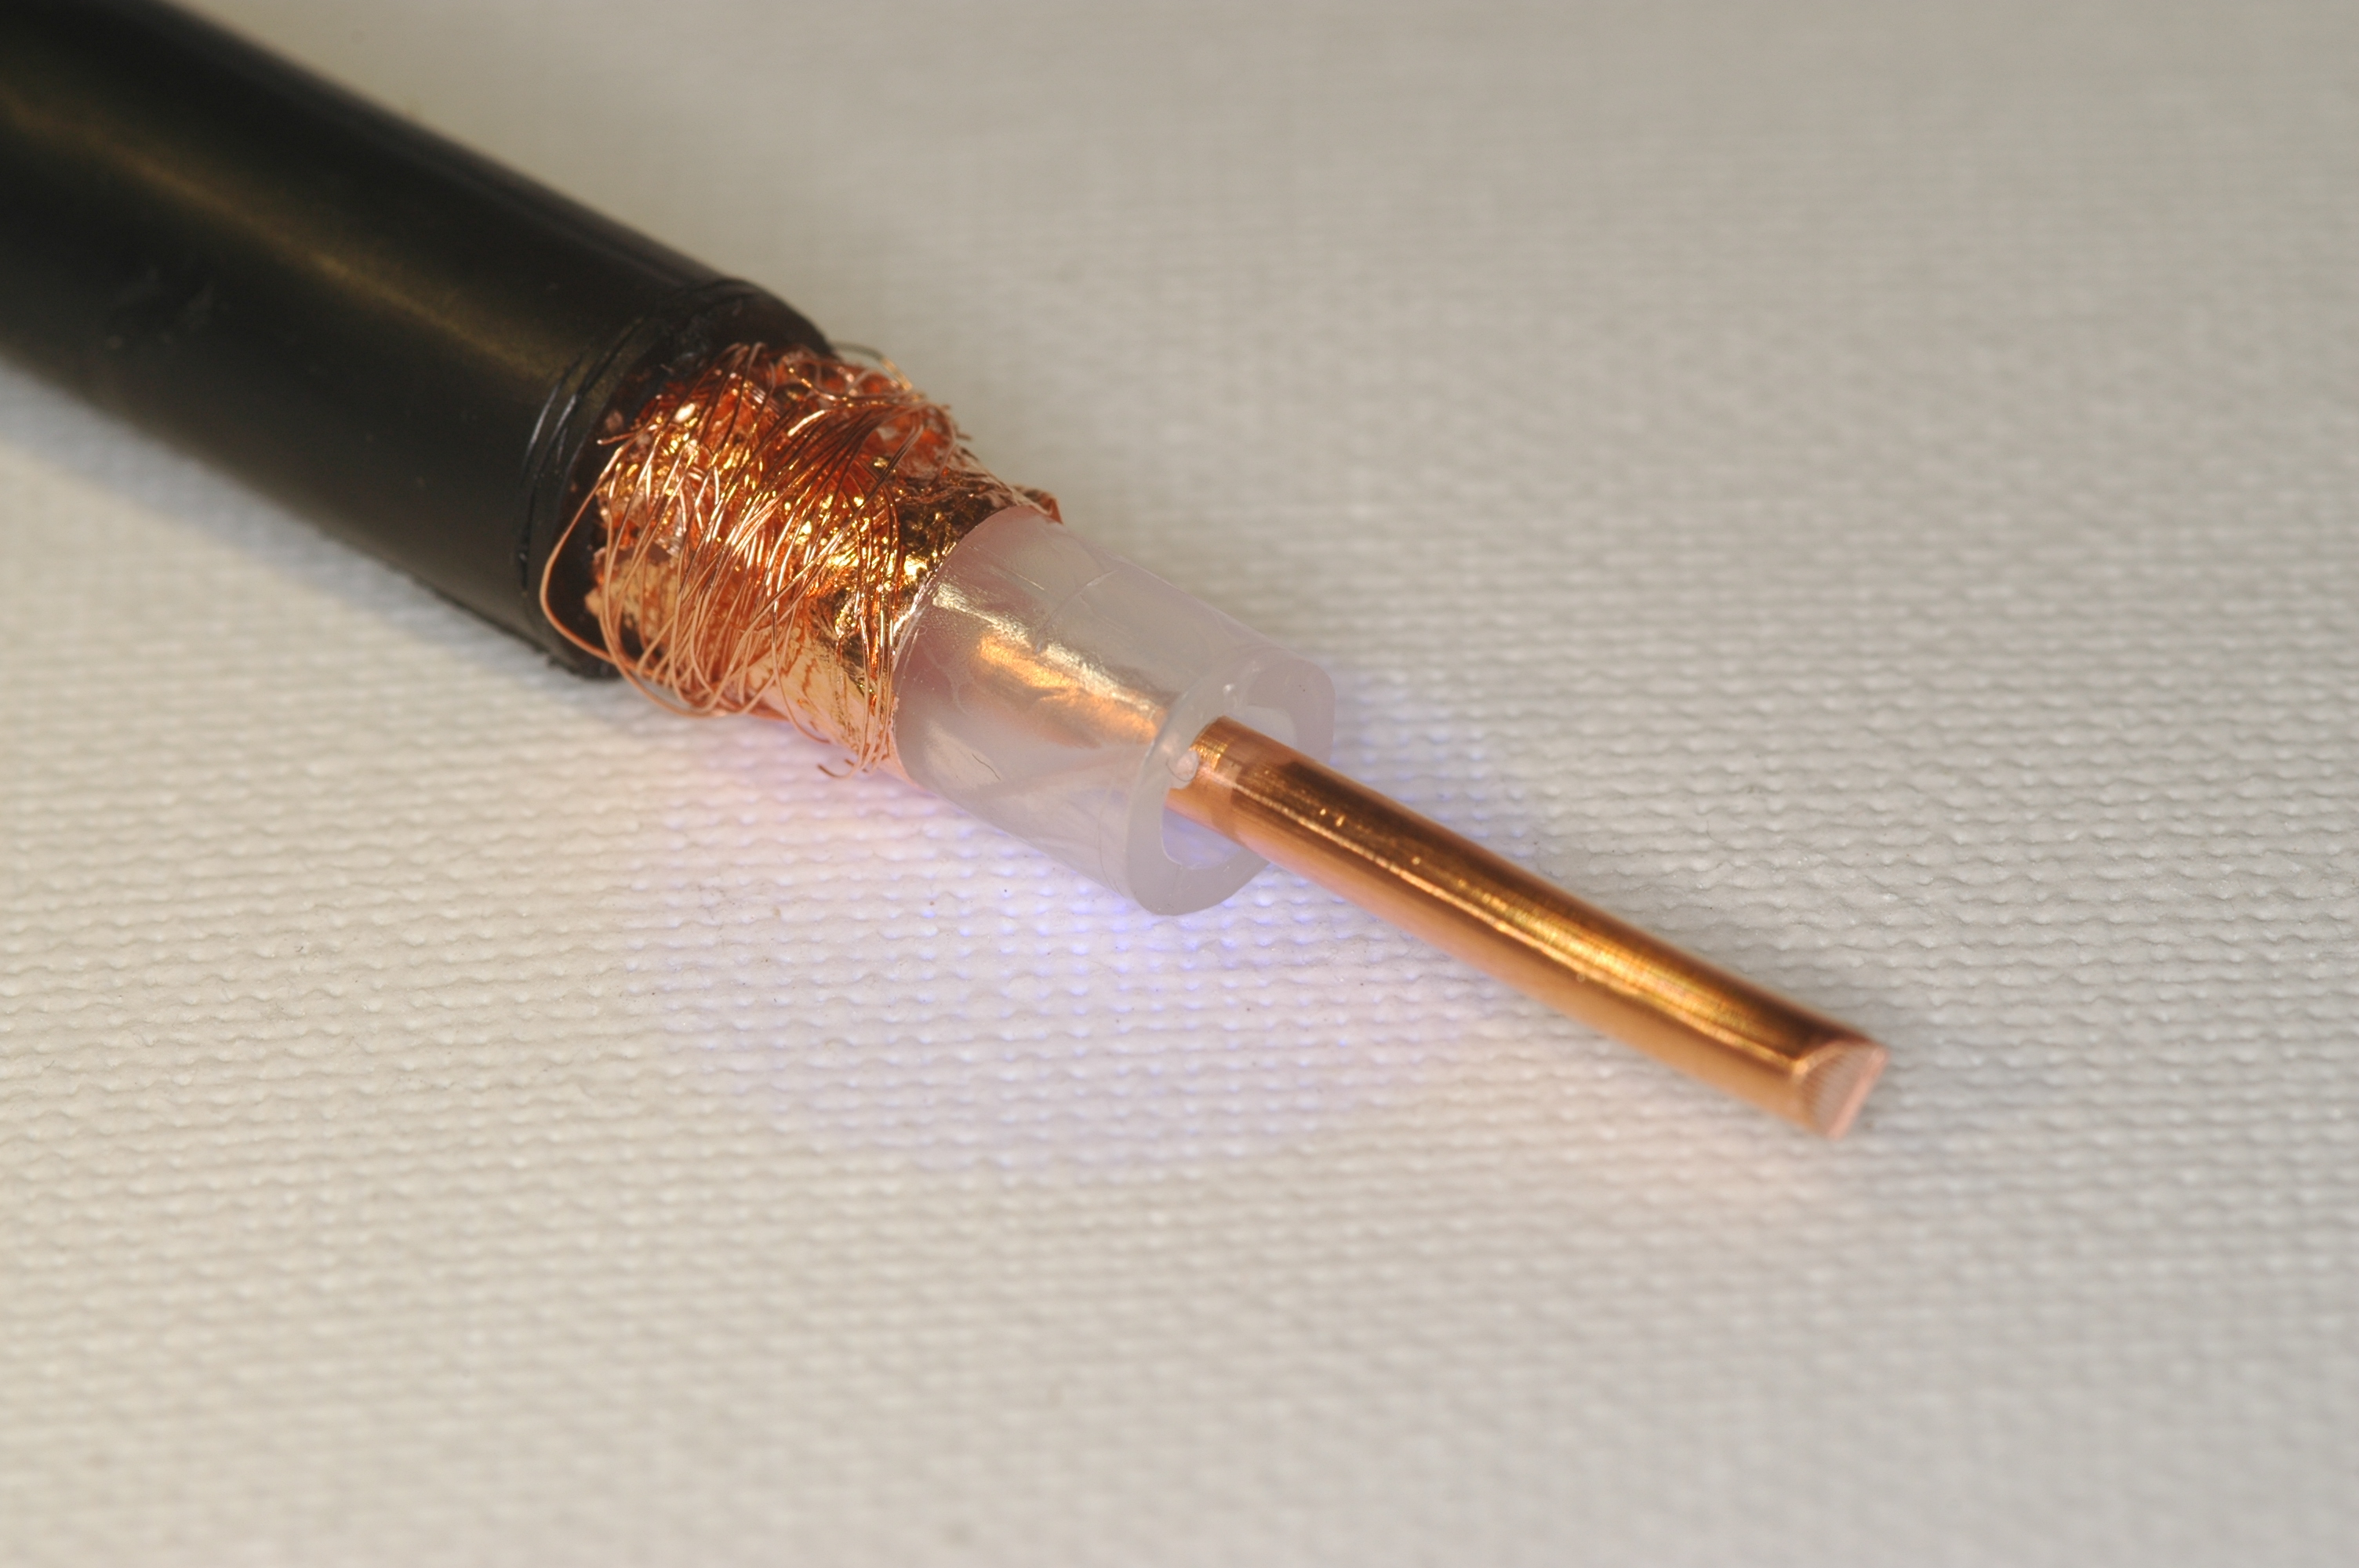
\includegraphics[width=0.85\textwidth]{foto/65}
    \caption{\scriptsize Geöffnetes Koaxialkabel aus Mantel, Schirmung, Dielektrikum und Innenleiter}
    \label{e_uebertragungsleitungen_koaxialkabel}
\end{figure}

    \end{column}
   \begin{column}{0.48\textwidth}
       \begin{itemize}
  \item Wie bei Antennen, ist eine Speiseleitung unsymmetrisch, wenn unterschiedliche Spannungen anliegen
  \item Beim Koaxialkabel sind die beiden Leiter unterschiedlich geformt
  \item Der Schirm weist gegenüber der Erde keine Spannung auf
  \end{itemize}

   \end{column}
\end{columns}

\end{frame}

\begin{frame}
\only<1>{
\begin{QQuestion}{EG304}{Wann ist eine Speiseleitung unsymmetrisch?}{Wenn die Länge nicht einem Vielfachen von $\lambda$/2 entspricht.}
{Wenn die hin- und zurücklaufende Leistung verschieden sind.}
{Wenn sie außerhalb ihrer Resonanzfrequenz betrieben wird.}
{Wenn die beiden Leiter unterschiedlich geformt sind, z. B. Koaxialkabel.}
\end{QQuestion}

}
\only<2>{
\begin{QQuestion}{EG304}{Wann ist eine Speiseleitung unsymmetrisch?}{Wenn die Länge nicht einem Vielfachen von $\lambda$/2 entspricht.}
{Wenn die hin- und zurücklaufende Leistung verschieden sind.}
{Wenn sie außerhalb ihrer Resonanzfrequenz betrieben wird.}
{\textbf{\textcolor{DARCgreen}{Wenn die beiden Leiter unterschiedlich geformt sind, z. B. Koaxialkabel.}}}
\end{QQuestion}

}
\end{frame}

\begin{frame}
\frametitle{Spannungsfestigkeit}
\begin{itemize}
  \item Im Koaxialkabel treten im Dielektrikum Verluste auf
  \item Es kann bei hohen Spannungen zu einem Durchschlag kommen
  \end{itemize}
\end{frame}

\begin{frame}
\only<1>{
\begin{QQuestion}{EG305}{Welche Vorteile hat eine Paralleldraht-Speiseleitung gegenüber der Speisung über ein Koaxialkabel?}{Sie hat geringere Dämpfung und hohe Spannungsfestigkeit.}
{Sie vermeidet Mantelwellen durch Wegfall der Abschirmung.}
{Sie erlaubt leichtere Kontrolle des Wellenwiderstandes durch Verschieben der Spreizer.}
{Sie bietet guten Blitzschutz durch niederohmige Drähte.}
\end{QQuestion}

}
\only<2>{
\begin{QQuestion}{EG305}{Welche Vorteile hat eine Paralleldraht-Speiseleitung gegenüber der Speisung über ein Koaxialkabel?}{\textbf{\textcolor{DARCgreen}{Sie hat geringere Dämpfung und hohe Spannungsfestigkeit.}}}
{Sie vermeidet Mantelwellen durch Wegfall der Abschirmung.}
{Sie erlaubt leichtere Kontrolle des Wellenwiderstandes durch Verschieben der Spreizer.}
{Sie bietet guten Blitzschutz durch niederohmige Drähte.}
\end{QQuestion}

}
\end{frame}

\begin{frame}
\frametitle{Koaxialstecker}
\begin{columns}
    \begin{column}{0.48\textwidth}
    
\begin{figure}
    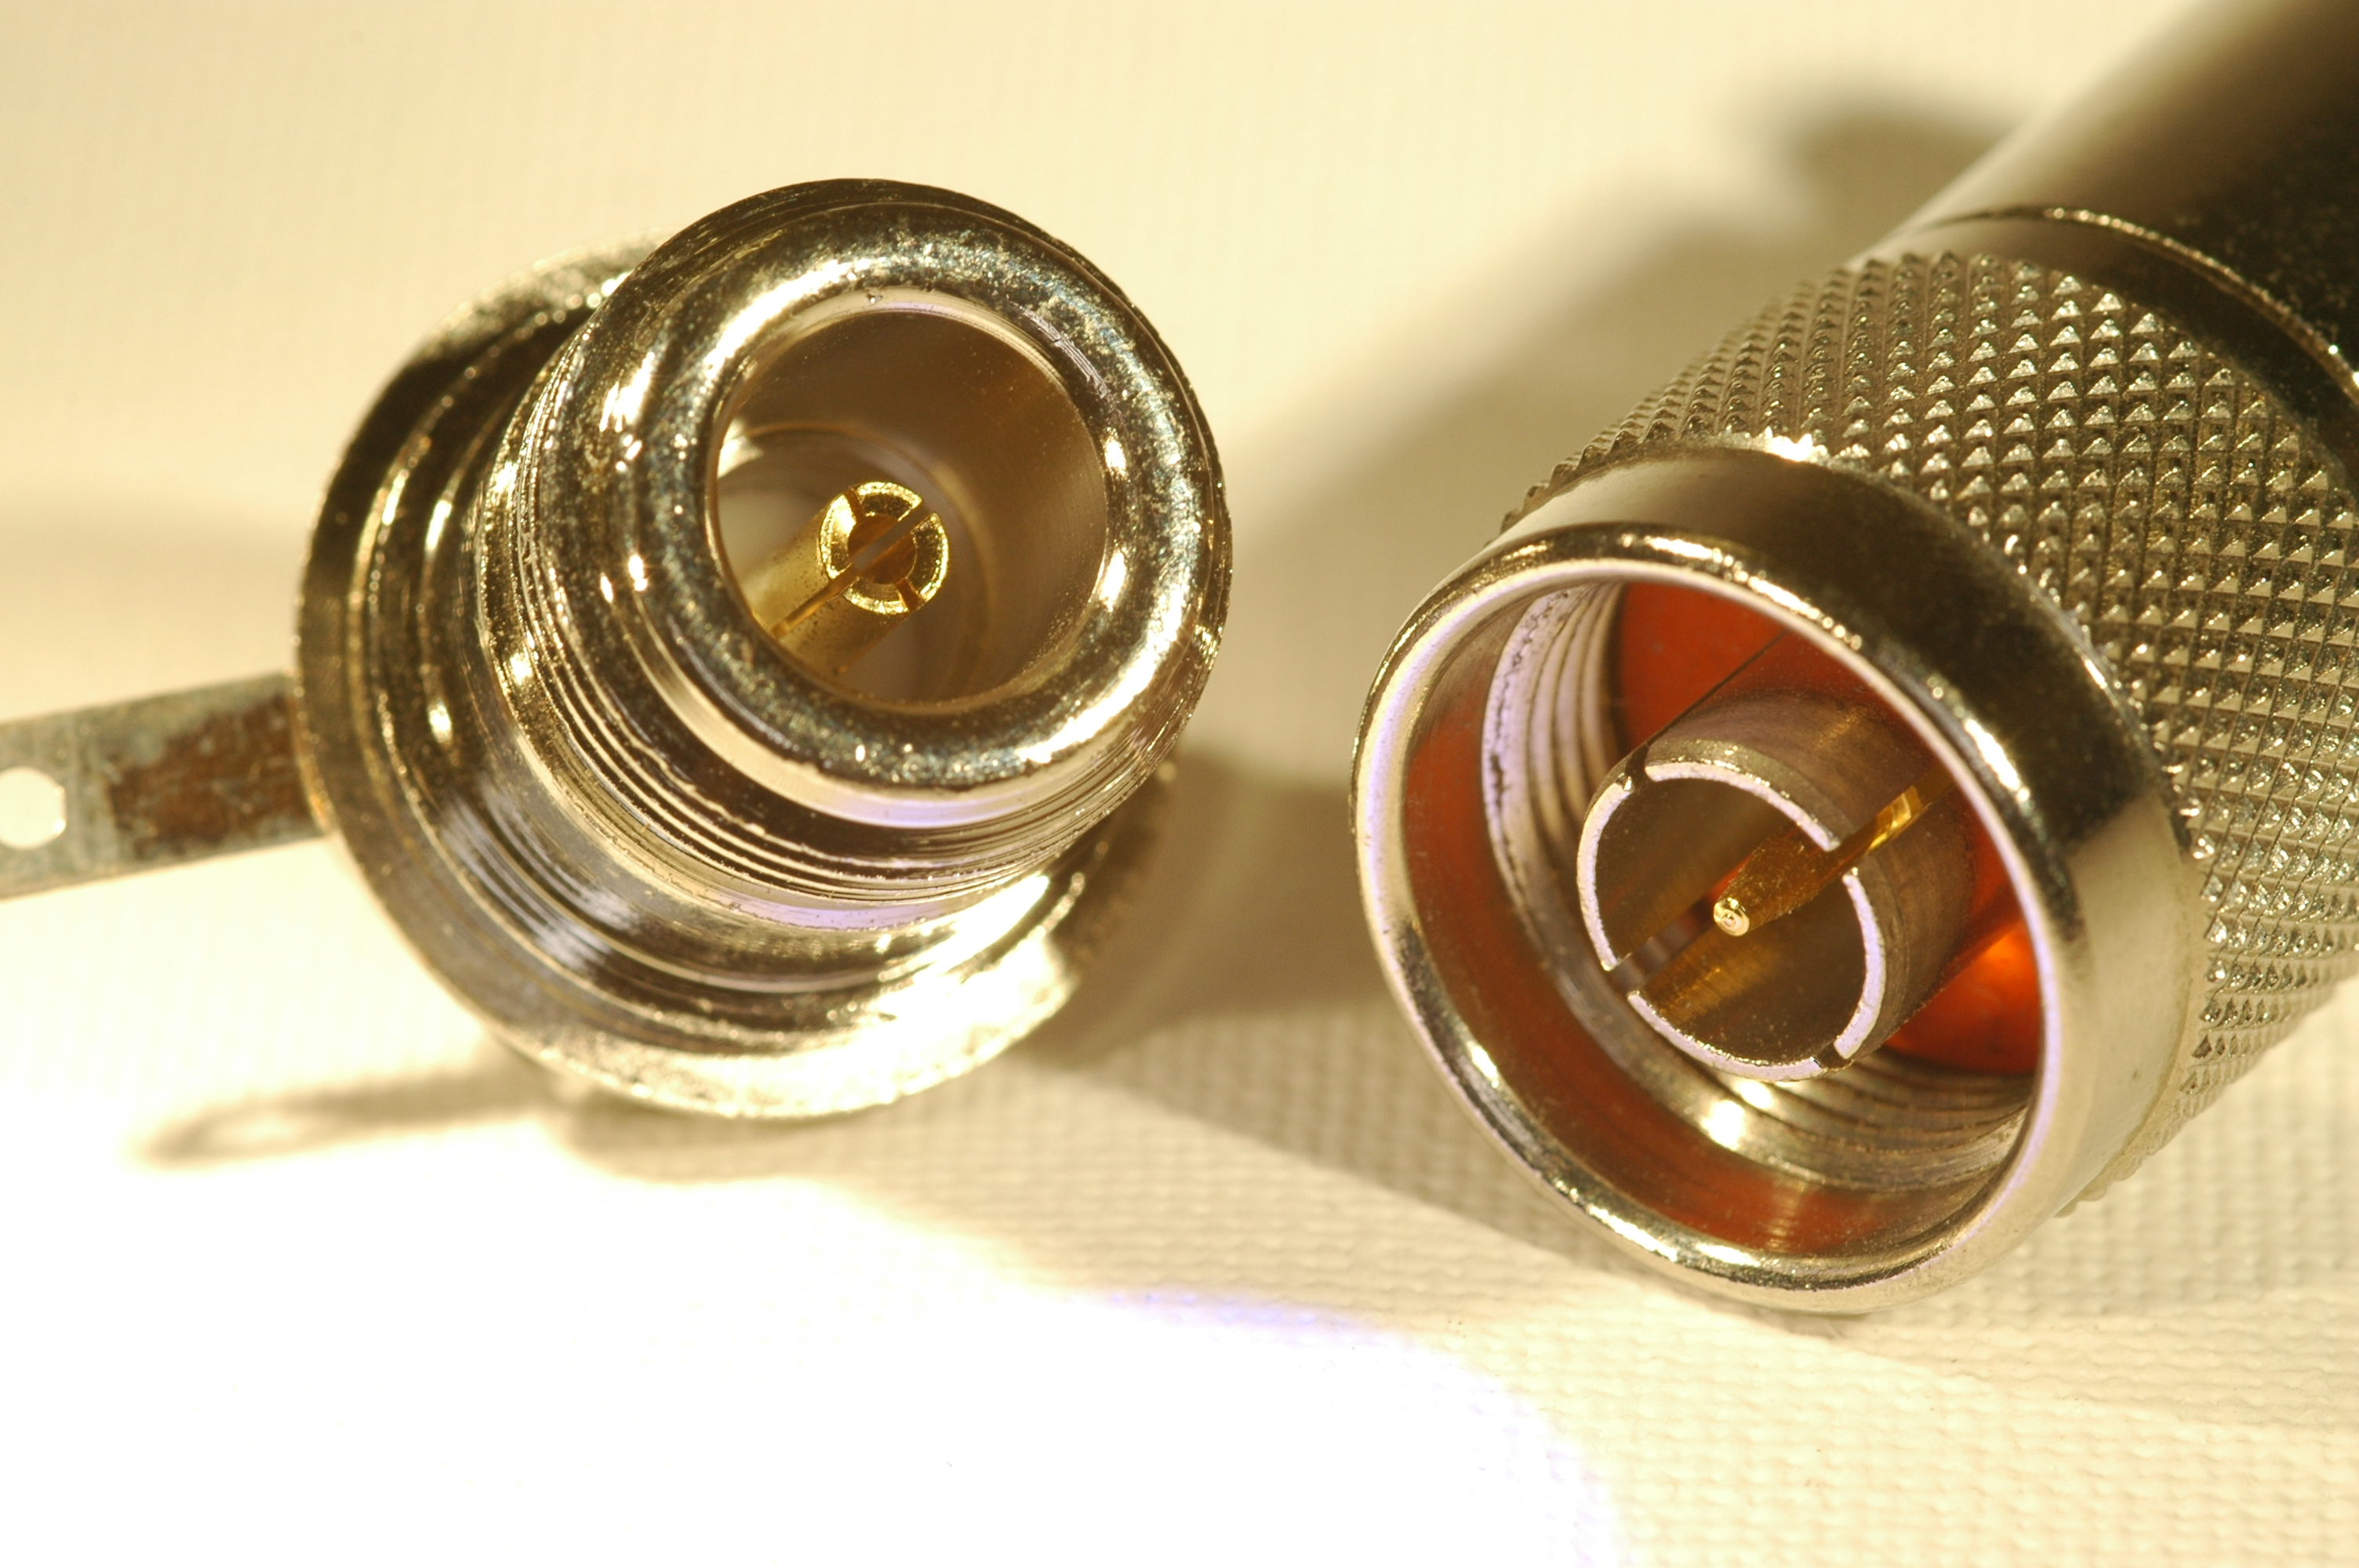
\includegraphics[width=0.85\textwidth]{foto/73}
    \caption{\scriptsize N-Buchse und N-Stecker}
    \label{e_uebertragungsleitungen_n_stecker_buchse}
\end{figure}

    \end{column}
   \begin{column}{0.48\textwidth}
       \begin{itemize}
  \item \emph{N-Stecker}: für niedrige und hohe Frequenz und hohe Leistung
  \item \emph{BNC-Stecker}: für niedrige und hohe Frequenz und geringe Leistung
  \item \emph{SMA-Stecker}: für hohe Frequenz und geringe Leistung
  \item \emph{UHF/PL-Stecker}: für niedrige Frequenz und hohe Leistung
  \end{itemize}

   \end{column}
\end{columns}

\end{frame}

\begin{frame}
\only<1>{
\begin{QQuestion}{EG303}{Welcher der folgenden Koaxialstecker besitzt einen definierten Wellenwiderstand von \qty{50}{\ohm} bis in den GHz-Bereich und hat die höchste Spannungsfestigkeit für die Übertragung hoher Leistungen?}{BNC-Stecker}
{SMA-Stecker}
{UHF-Stecker}
{N-Stecker}
\end{QQuestion}

}
\only<2>{
\begin{QQuestion}{EG303}{Welcher der folgenden Koaxialstecker besitzt einen definierten Wellenwiderstand von \qty{50}{\ohm} bis in den GHz-Bereich und hat die höchste Spannungsfestigkeit für die Übertragung hoher Leistungen?}{BNC-Stecker}
{SMA-Stecker}
{UHF-Stecker}
{\textbf{\textcolor{DARCgreen}{N-Stecker}}}
\end{QQuestion}

}
\end{frame}%ENDCONTENT


\section{Kabeldämpfung I}
\label{section:kabeldaempfung_1}
\begin{frame}%STARTCONTENT
\begin{itemize}
  \item Signalstärke eines Hochfrequenzsignals nimmt bei zunehmender Kabellänge ab
  \item Wird als \emph{Kabeldämpfung} bezeichnet
  \item Auch Stecker können das Signal dämpfen
  \item Ist unerwünscht
  \end{itemize}
\end{frame}

\begin{frame}
\begin{columns}
    \begin{column}{0.48\textwidth}
    \begin{itemize}
  \item Dämpfung wird in der Regel in Dezibel (dB) angegeben
  \item Wenn von Dämpfung gesprochen wird, bleibt die Zahl positiv
  \end{itemize}

    \end{column}
   \begin{column}{0.48\textwidth}
       \begin{itemize}
  \item Faktor zu dB-Umrechnung verwenden
  \item Oder in der Formelsammlung nachschlagen
  \end{itemize}

   \end{column}
\end{columns}

\end{frame}

\begin{frame}
\only<1>{
\begin{QQuestion}{EG309}{Am Ende einer Antennenleitung ist nur noch ein Viertel der Leistung vorhanden. Wie groß ist das Dämpfungsmaß des Kabels?}{\qty{3}{\decibel}}
{\qty{6}{\decibel}}
{\qty{10}{\decibel}}
{\qty{16}{\decibel}}
\end{QQuestion}

}
\only<2>{
\begin{QQuestion}{EG309}{Am Ende einer Antennenleitung ist nur noch ein Viertel der Leistung vorhanden. Wie groß ist das Dämpfungsmaß des Kabels?}{\qty{3}{\decibel}}
{\textbf{\textcolor{DARCgreen}{\qty{6}{\decibel}}}}
{\qty{10}{\decibel}}
{\qty{16}{\decibel}}
\end{QQuestion}

}
\end{frame}

\begin{frame}
\only<1>{
\begin{QQuestion}{EG310}{Am Ende einer Antennenleitung ist nur noch ein Zehntel der Leistung vorhanden. Wie groß ist das Dämpfungsmaß des Kabels?}{\qty{3}{\decibel}}
{\qty{10}{\decibel}}
{\qty{6}{\decibel}}
{\qty{16}{\decibel}}
\end{QQuestion}

}
\only<2>{
\begin{QQuestion}{EG310}{Am Ende einer Antennenleitung ist nur noch ein Zehntel der Leistung vorhanden. Wie groß ist das Dämpfungsmaß des Kabels?}{\qty{3}{\decibel}}
{\textbf{\textcolor{DARCgreen}{\qty{10}{\decibel}}}}
{\qty{6}{\decibel}}
{\qty{16}{\decibel}}
\end{QQuestion}

}
\end{frame}

\begin{frame}
\only<1>{
\begin{QQuestion}{EG308}{Eine HF-Ausgangsleistung von \qty{100}{\W} wird in eine angepasste Übertragungsleitung eingespeist. Am antennenseitigen Ende der Leitung beträgt die Leistung \qty{50}{\W} bei einem SWR von 1. Wie hoch ist die Leitungsdämpfung?}{\qty{-3}{\decibel}}
{\qty{-6}{\decibel}}
{\qty{3}{\decibel}}
{\qty{6}{\dBm}}
\end{QQuestion}

}
\only<2>{
\begin{QQuestion}{EG308}{Eine HF-Ausgangsleistung von \qty{100}{\W} wird in eine angepasste Übertragungsleitung eingespeist. Am antennenseitigen Ende der Leitung beträgt die Leistung \qty{50}{\W} bei einem SWR von 1. Wie hoch ist die Leitungsdämpfung?}{\qty{-3}{\decibel}}
{\qty{-6}{\decibel}}
{\textbf{\textcolor{DARCgreen}{\qty{3}{\decibel}}}}
{\qty{6}{\dBm}}
\end{QQuestion}

}
\end{frame}

\begin{frame}
\frametitle{Kabelverluste}
\begin{itemize}
  \item Alle Verluste, die in Kabeln entstehen
  \item Antenne und Verstärker verstärken das Signal, verändern jedoch nicht die Kabelverluste
  \end{itemize}
\end{frame}

\begin{frame}
\only<1>{
\begin{PQuestion}{EG307}{Die Skizze zeigt den Aufbau einer Amateurfunkstelle. Die Summe aller Kabelverluste in Dezibel betragen~...}{\qty{3}{\decibel}}
{\qty{-5}{\decibel}}
{\qty{5}{\decibel}}
{\qty{-3}{\decibel}}
{\DARCimage{1.0\linewidth}{439include}}\end{PQuestion}

}
\only<2>{
\begin{PQuestion}{EG307}{Die Skizze zeigt den Aufbau einer Amateurfunkstelle. Die Summe aller Kabelverluste in Dezibel betragen~...}{\qty{3}{\decibel}}
{\qty{-5}{\decibel}}
{\textbf{\textcolor{DARCgreen}{\qty{5}{\decibel}}}}
{\qty{-3}{\decibel}}
{\DARCimage{1.0\linewidth}{439include}}\end{PQuestion}

}
\end{frame}

\begin{frame}
\frametitle{Kabeldämpfungsdiagramm}
\begin{columns}
    \begin{column}{0.48\textwidth}
    \begin{itemize}
  \item Im Anhang der Formelsammlung
  \item Dämpfungen verschiedener Kabel in Abhängigkeit zur Frequenz
  \item Bezug auf 100m -- bei kürzeren Kabeln muss umgerechnet werden
  \end{itemize}

    \end{column}
   \begin{column}{0.48\textwidth}
       
\begin{figure}
    \DARCimage{0.85\linewidth}{202include}
    \caption{\scriptsize Kabeldämpfungsdiagramm im Anhang der Formelsammlung}
    \label{e_kabeldaempfung_diagramm}
\end{figure}


   \end{column}
\end{columns}

\end{frame}

\begin{frame}
\only<1>{
\begin{QQuestion}{EG312}{Welche Dämpfung ergibt sich auf der Grundlage des Kabeldämpfungsdiagramms für ein \qty{100}{\m} langes Koaxialkabel mit Voll-PE-Dielektrikum, \qty{4,95}{\mm} Durchmesser (Typ RG58), bei \qty{145}{\MHz}?}{\qty{0}{\decibel}}
{\qty{39}{\decibel}}
{\qty{1}{\decibel}}
{\qty{20}{\decibel}}
\end{QQuestion}

}
\only<2>{
\begin{QQuestion}{EG312}{Welche Dämpfung ergibt sich auf der Grundlage des Kabeldämpfungsdiagramms für ein \qty{100}{\m} langes Koaxialkabel mit Voll-PE-Dielektrikum, \qty{4,95}{\mm} Durchmesser (Typ RG58), bei \qty{145}{\MHz}?}{\qty{0}{\decibel}}
{\qty{39}{\decibel}}
{\qty{1}{\decibel}}
{\textbf{\textcolor{DARCgreen}{\qty{20}{\decibel}}}}
\end{QQuestion}

}
\end{frame}

\begin{frame}
\frametitle{Lösungsweg}
\begin{itemize}
  \item gesucht: Dämpfung für 100m RG58 Kabel bei \qty{145}{\mega\hertz}
  \item Lösung: Ablesen aus Diagramm
  \item Schnittpunkt der RG58 Linie mit \qty{145}{\mega\hertz} $\rightarrow$ \qty{20}{\dB}
  \end{itemize}
\end{frame}

\begin{frame}
\only<1>{
\begin{QQuestion}{EG311}{Ein \qty{100}{\m} langes Koaxialkabel hat eine Dämpfung von \qty{20}{\decibel} bei \qty{145}{\MHz}. Wie hoch ist die Dämpfung bei einer Länge von \qty{20}{\m}?}{\qty{5}{\decibel}}
{\qty{7,25}{\decibel}}
{\qty{4}{\decibel}}
{\qty{1,45}{\decibel}}
\end{QQuestion}

}
\only<2>{
\begin{QQuestion}{EG311}{Ein \qty{100}{\m} langes Koaxialkabel hat eine Dämpfung von \qty{20}{\decibel} bei \qty{145}{\MHz}. Wie hoch ist die Dämpfung bei einer Länge von \qty{20}{\m}?}{\qty{5}{\decibel}}
{\qty{7,25}{\decibel}}
{\textbf{\textcolor{DARCgreen}{\qty{4}{\decibel}}}}
{\qty{1,45}{\decibel}}
\end{QQuestion}

}
\end{frame}

\begin{frame}
\frametitle{Lösungsweg}
\begin{itemize}
  \item gesucht: Dämpfung für 20m bei 20dB Dämpfung auf 100m
  \item Lösung: Dreisatz
  \end{itemize}
$\dfrac{20dB}{100m} = \dfrac{x}{20m}$

$x = \dfrac{20dB\cdot 20m}{100m} = 4dB$

\end{frame}

\begin{frame}
\only<1>{
\begin{QQuestion}{EG313}{Welche Dämpfung ergibt sich auf der Grundlage des Kabeldämpfungsdiagramms für ein \qty{15}{\m} langes Koaxialkabel mit Voll-PE-Dielektrikum, \qty{4,95}{\mm} Durchmesser (Typ RG58), bei \qty{145}{\MHz}?}{\qty{2}{\decibel}}
{\qty{4}{\decibel}}
{\qty{3}{\decibel}}
{\qty{1}{\decibel}}
\end{QQuestion}

}
\only<2>{
\begin{QQuestion}{EG313}{Welche Dämpfung ergibt sich auf der Grundlage des Kabeldämpfungsdiagramms für ein \qty{15}{\m} langes Koaxialkabel mit Voll-PE-Dielektrikum, \qty{4,95}{\mm} Durchmesser (Typ RG58), bei \qty{145}{\MHz}?}{\qty{2}{\decibel}}
{\qty{4}{\decibel}}
{\textbf{\textcolor{DARCgreen}{\qty{3}{\decibel}}}}
{\qty{1}{\decibel}}
\end{QQuestion}

}
\end{frame}

\begin{frame}
\frametitle{Lösungsweg}
\begin{itemize}
  \item gesucht: Dämpfung für 15m RG58 Kabel bei \qty{145}{\mega\hertz}
  \item Lösung: Ablesen aus Diagramm und Dreisatz
  \item Schnittpunkt der RG58 Linie mit \qty{145}{\mega\hertz} $\rightarrow$ \qty{20}{\dB}
  \end{itemize}
$\dfrac{20dB}{100m} = \dfrac{x}{15m}$

$x = \dfrac{20dB\cdot 15m}{100m} = 3dB$

\end{frame}

\begin{frame}
\only<1>{
\begin{QQuestion}{EG314}{Welche Dämpfung ergibt sich auf der Grundlage des Kabeldämpfungsdiagramms für ein \qty{50}{\m} langes Koaxialkabel mit Voll-PE-Dielektrikum, \qty{2,8}{\mm} Durchmesser (Typ RG174), bei \qty{145}{\MHz}?}{\qty{12}{\decibel}}
{\qty{40}{\decibel}}
{\qty{68}{\decibel}}
{\qty{20}{\decibel}}
\end{QQuestion}

}
\only<2>{
\begin{QQuestion}{EG314}{Welche Dämpfung ergibt sich auf der Grundlage des Kabeldämpfungsdiagramms für ein \qty{50}{\m} langes Koaxialkabel mit Voll-PE-Dielektrikum, \qty{2,8}{\mm} Durchmesser (Typ RG174), bei \qty{145}{\MHz}?}{\qty{12}{\decibel}}
{\qty{40}{\decibel}}
{\qty{68}{\decibel}}
{\textbf{\textcolor{DARCgreen}{\qty{20}{\decibel}}}}
\end{QQuestion}

}
\end{frame}

\begin{frame}
\only<1>{
\begin{QQuestion}{EG315}{Welche Dämpfung ergibt sich auf der Grundlage des Kabeldämpfungsdiagramms für ein \qty{40}{\m} langes Koaxialkabel, PE-Schaum-Dielektrikum mit \qty{12,7}{\mm} Durchmesser, bei \qty{435}{\MHz}?}{\qty{0,8}{\decibel}}
{\qty{3,8}{\decibel}}
{\qty{1,8}{\decibel}}
{\qty{2,8}{\decibel}}
\end{QQuestion}

}
\only<2>{
\begin{QQuestion}{EG315}{Welche Dämpfung ergibt sich auf der Grundlage des Kabeldämpfungsdiagramms für ein \qty{40}{\m} langes Koaxialkabel, PE-Schaum-Dielektrikum mit \qty{12,7}{\mm} Durchmesser, bei \qty{435}{\MHz}?}{\qty{0,8}{\decibel}}
{\qty{3,8}{\decibel}}
{\qty{1,8}{\decibel}}
{\textbf{\textcolor{DARCgreen}{\qty{2,8}{\decibel}}}}
\end{QQuestion}

}
\end{frame}

\begin{frame}
\only<1>{
\begin{QQuestion}{EG316}{Welche Dämpfung ergibt sich auf der Grundlage des Kabeldämpfungsdiagramms für ein \qty{40}{\m} langes Koaxialkabel mit PE-Schaum-Dielektrikum und \qty{10,3}{\mm} Durchmesser im \qty{23}{\cm}-Band (\qty{1296}{\MHz})?}{\qty{8,2}{\decibel}}
{\qty{12,6}{\decibel}}
{\qty{10,4}{\decibel}}
{\qty{6,2}{\decibel}}
\end{QQuestion}

}
\only<2>{
\begin{QQuestion}{EG316}{Welche Dämpfung ergibt sich auf der Grundlage des Kabeldämpfungsdiagramms für ein \qty{40}{\m} langes Koaxialkabel mit PE-Schaum-Dielektrikum und \qty{10,3}{\mm} Durchmesser im \qty{23}{\cm}-Band (\qty{1296}{\MHz})?}{\textbf{\textcolor{DARCgreen}{\qty{8,2}{\decibel}}}}
{\qty{12,6}{\decibel}}
{\qty{10,4}{\decibel}}
{\qty{6,2}{\decibel}}
\end{QQuestion}

}
\end{frame}%ENDCONTENT


\section{Stehwellenverhältnis (SWR) II}
\label{section:swr_2}
\begin{frame}%STARTCONTENT
\begin{itemize}
  \item Stehwellenverhältnis: Vorlaufende zu rücklaufender Energie
  \item SWR von 3 bei \qty{100}{\watt}: \qty{75}{\watt} werden abgestrahlt, \qty{25}{\watt} laufen zurück
  \item Oder auch: \qty{75}{\percent} gehen auf die Antenne, \qty{25}{\percent} werden reflektiert
  \end{itemize}
\end{frame}

\begin{frame}
\only<1>{
\begin{QQuestion}{EG401}{Am Eingang einer Antennenleitung misst man ein SWR von~3. Wie groß ist dort in etwa die rücklaufende Leistung, wenn die vorlaufende Leistung \qty{100}{\W} beträgt?}{\qty{75}{\W}}
{\qty{12,5}{\W}}
{\qty{50}{\W}}
{\qty{25}{\W}}
\end{QQuestion}

}
\only<2>{
\begin{QQuestion}{EG401}{Am Eingang einer Antennenleitung misst man ein SWR von~3. Wie groß ist dort in etwa die rücklaufende Leistung, wenn die vorlaufende Leistung \qty{100}{\W} beträgt?}{\qty{75}{\W}}
{\qty{12,5}{\W}}
{\qty{50}{\W}}
{\textbf{\textcolor{DARCgreen}{\qty{25}{\W}}}}
\end{QQuestion}

}
\end{frame}

\begin{frame}
\only<1>{
\begin{QQuestion}{EG402}{Sie messen ein Stehwellenverhältnis (SWR) von 3. Wieviel Prozent der vorlaufenden Leistung werden reflektiert?}{\qty{25}{\percent}}
{\qty{33}{\percent}}
{\qty{50}{\percent}}
{\qty{75}{\percent}}
\end{QQuestion}

}
\only<2>{
\begin{QQuestion}{EG402}{Sie messen ein Stehwellenverhältnis (SWR) von 3. Wieviel Prozent der vorlaufenden Leistung werden reflektiert?}{\textbf{\textcolor{DARCgreen}{\qty{25}{\percent}}}}
{\qty{33}{\percent}}
{\qty{50}{\percent}}
{\qty{75}{\percent}}
\end{QQuestion}

}
\end{frame}

\begin{frame}
\only<1>{
\begin{QQuestion}{EG403}{Sie messen ein Stehwellenverhältnis (SWR) von 3. Wieviel Prozent der vorlaufenden Leistung werden abgegeben?}{\qty{75}{\percent}}
{\qty{50}{\percent}}
{\qty{25}{\percent}}
{\qty{29}{\percent}}
\end{QQuestion}

}
\only<2>{
\begin{QQuestion}{EG403}{Sie messen ein Stehwellenverhältnis (SWR) von 3. Wieviel Prozent der vorlaufenden Leistung werden abgegeben?}{\textbf{\textcolor{DARCgreen}{\qty{75}{\percent}}}}
{\qty{50}{\percent}}
{\qty{25}{\percent}}
{\qty{29}{\percent}}
\end{QQuestion}

}
\end{frame}%ENDCONTENT


\section{Stehwellenmessgerät (SWR-Meter) I}
\label{section:swr_meter_1}
\begin{frame}%STARTCONTENT

\begin{columns}
    \begin{column}{0.48\textwidth}
    \begin{itemize}
  \item Misst die Leitungsanpassung
  \item Wie gut stimmt der Wellenwiderstand mit dem Speisewiderstand der Antenne oder der Impedanz des Transceivers überein?
  \item Wird auch SWR-Messbrücke genannt
  \end{itemize}

    \end{column}
   \begin{column}{0.48\textwidth}
       
\begin{figure}
    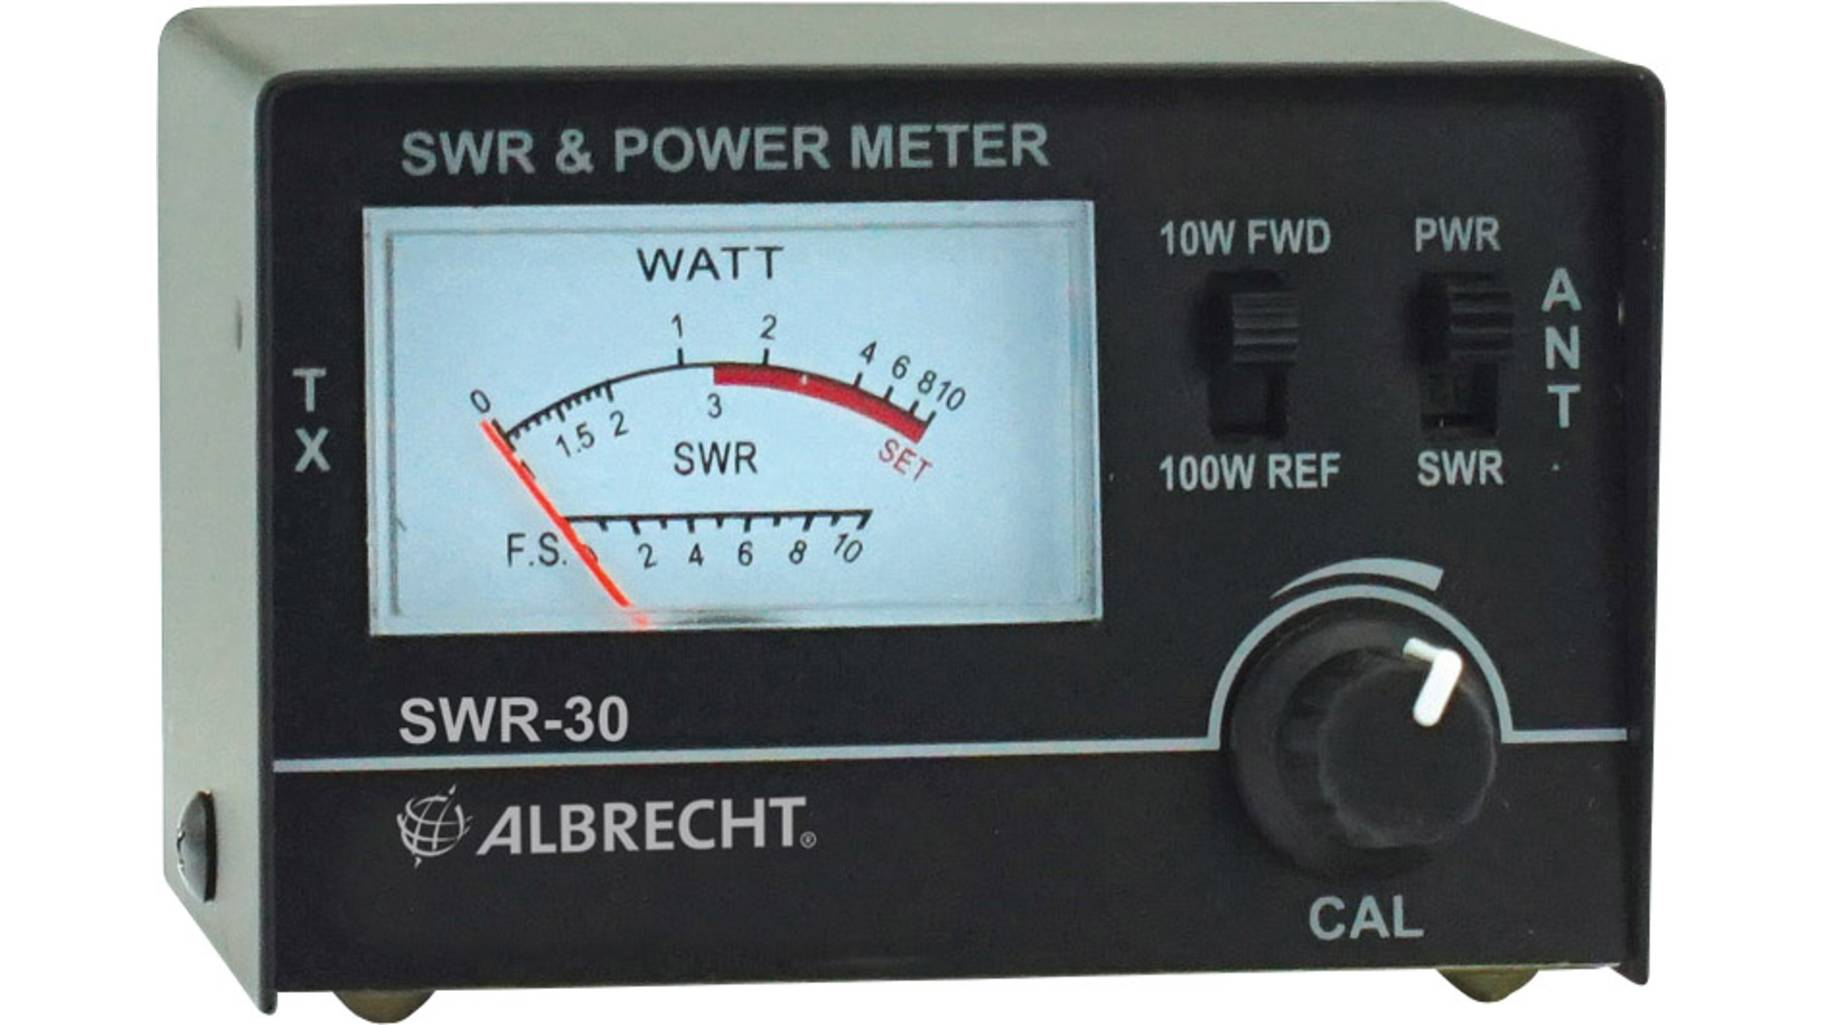
\includegraphics[width=0.85\textwidth]{foto/144}
    \caption{\scriptsize Ein SWR-Meter zur Messung bis maximal \qty{100}{\watt}}
    \label{e_swr_meter_geraet}
\end{figure}

   \end{column}
\end{columns}

\end{frame}

\begin{frame}
\only<1>{
\begin{QQuestion}{EI401}{Ein Stehwellenmessgerät wird eingesetzt bei Sendern zur Messung~...}{der Bandbreite.}
{der Oberwellenausgangsleistung.}
{der Antennenanpassung.}
{des Wirkungsgrades.}
\end{QQuestion}

}
\only<2>{
\begin{QQuestion}{EI401}{Ein Stehwellenmessgerät wird eingesetzt bei Sendern zur Messung~...}{der Bandbreite.}
{der Oberwellenausgangsleistung.}
{\textbf{\textcolor{DARCgreen}{der Antennenanpassung.}}}
{des Wirkungsgrades.}
\end{QQuestion}

}
\end{frame}

\begin{frame}
\only<1>{
\begin{QQuestion}{EI402}{Mit welchem Instrument kann die Anpassung zwischen einem UHF-Sender und der Speiseleitung zur Antenne angezeigt werden?}{Interferometer}
{Universalmessgerät mit Widerstandsanzeige}
{SWR-Meter}
{Anpassungsübertrager}
\end{QQuestion}

}
\only<2>{
\begin{QQuestion}{EI402}{Mit welchem Instrument kann die Anpassung zwischen einem UHF-Sender und der Speiseleitung zur Antenne angezeigt werden?}{Interferometer}
{Universalmessgerät mit Widerstandsanzeige}
{\textbf{\textcolor{DARCgreen}{SWR-Meter}}}
{Anpassungsübertrager}
\end{QQuestion}

}
\end{frame}

\begin{frame}
\only<1>{
\begin{QQuestion}{EI403}{Wie misst man das Stehwellenverhältnis im Sendebetrieb? Man misst es~...}{durch Spannungsmessung am Anfang und am Ende der Speiseleitung.}
{mit einem Absorptionswellenmesser.}
{durch Strommessung am Anfang und am Ende der Speiseleitung.}
{mit einer SWR-Messbrücke.}
\end{QQuestion}

}
\only<2>{
\begin{QQuestion}{EI403}{Wie misst man das Stehwellenverhältnis im Sendebetrieb? Man misst es~...}{durch Spannungsmessung am Anfang und am Ende der Speiseleitung.}
{mit einem Absorptionswellenmesser.}
{durch Strommessung am Anfang und am Ende der Speiseleitung.}
{\textbf{\textcolor{DARCgreen}{mit einer SWR-Messbrücke.}}}
\end{QQuestion}

}
\end{frame}

\begin{frame}
\begin{columns}
    \begin{column}{0.48\textwidth}
    \begin{itemize}
  \item Messung der Antennenanpassung: So nah wie möglich an die Antenne, um Veränderungen der Speiseleitung auszuschließen
  \item Messung der gesamten Anlage: So nah wie möglich hinter dem Sender
  \end{itemize}

    \end{column}
   \begin{column}{0.48\textwidth}
       
\begin{figure}
    \DARCimage{0.85\linewidth}{670include}
    \caption{\scriptsize Prinzip der Messung eines SWR-Meters}
    \label{e_swr_meter_messung}
\end{figure}


   \end{column}
\end{columns}

\end{frame}

\begin{frame}
\only<1>{
\begin{QQuestion}{EI404}{An welcher Stelle muss ein SWR-Meter eingeschleift werden, um möglichst genaue Aussagen über die Antenne machen zu können? Das SWR-Meter muss eingeschleift werden zwischen~...}{Zwischen Anpassgerät und Antennenkabel.}
{Senderausgang und Antennenkabel.}
{Antennenkabel und Antenne.}
{Senderausgang und Antennenanpassgerät.}
\end{QQuestion}

}
\only<2>{
\begin{QQuestion}{EI404}{An welcher Stelle muss ein SWR-Meter eingeschleift werden, um möglichst genaue Aussagen über die Antenne machen zu können? Das SWR-Meter muss eingeschleift werden zwischen~...}{Zwischen Anpassgerät und Antennenkabel.}
{Senderausgang und Antennenkabel.}
{\textbf{\textcolor{DARCgreen}{Antennenkabel und Antenne.}}}
{Senderausgang und Antennenanpassgerät.}
\end{QQuestion}

}
\end{frame}

\begin{frame}
\only<1>{
\begin{PQuestion}{EI405}{An welchem Punkt sollte das Stehwellenmessgerät eingeschleift werden, um zu prüfen, ob die Antennenanlage gut an den Sender angepasst ist? }{Punkt 4}
{Punkt 2}
{Punkt 3}
{Punkt 1}
{\DARCimage{1.0\linewidth}{105include}}\end{PQuestion}

}
\only<2>{
\begin{PQuestion}{EI405}{An welchem Punkt sollte das Stehwellenmessgerät eingeschleift werden, um zu prüfen, ob die Antennenanlage gut an den Sender angepasst ist? }{Punkt 4}
{Punkt 2}
{Punkt 3}
{\textbf{\textcolor{DARCgreen}{Punkt 1}}}
{\DARCimage{1.0\linewidth}{105include}}\end{PQuestion}

}
\end{frame}%ENDCONTENT


\section{Vektorieller Netzwerkanalysator (VNA) I}
\label{section:vna_1}
\begin{frame}%STARTCONTENT

\begin{columns}
    \begin{column}{0.48\textwidth}
    \begin{itemize}
  \item Ein einfaches Multimeter kann keine frequenzabhängigen Widerstände messen
  \item Dazu wird ein \emph{vektorieller Netzwerkanalysator (VNA)} verwendet
  \end{itemize}

    \end{column}
   \begin{column}{0.48\textwidth}
       \begin{itemize}
  \item Aktives Messgerät
  \item Misst das Verhältnis von Spannung und Strom bei einer Frequenz
  \item Oft kann ein Frequenzbereich angegeben werden
  \end{itemize}

   \end{column}
\end{columns}

\end{frame}

\begin{frame}
\frametitle{Anwendungen}
\begin{columns}
    \begin{column}{0.48\textwidth}
    \begin{itemize}
  \item Große und kleine Widerstände eines Schwingkreis
  \item Resonanzfrequenz eines Schwingkreis
  \item Filterverhalten
  \item Impedanzmessung
  \item Stehwellenverhältnisse
  \end{itemize}

    \end{column}
   \begin{column}{0.48\textwidth}
       
\begin{figure}
    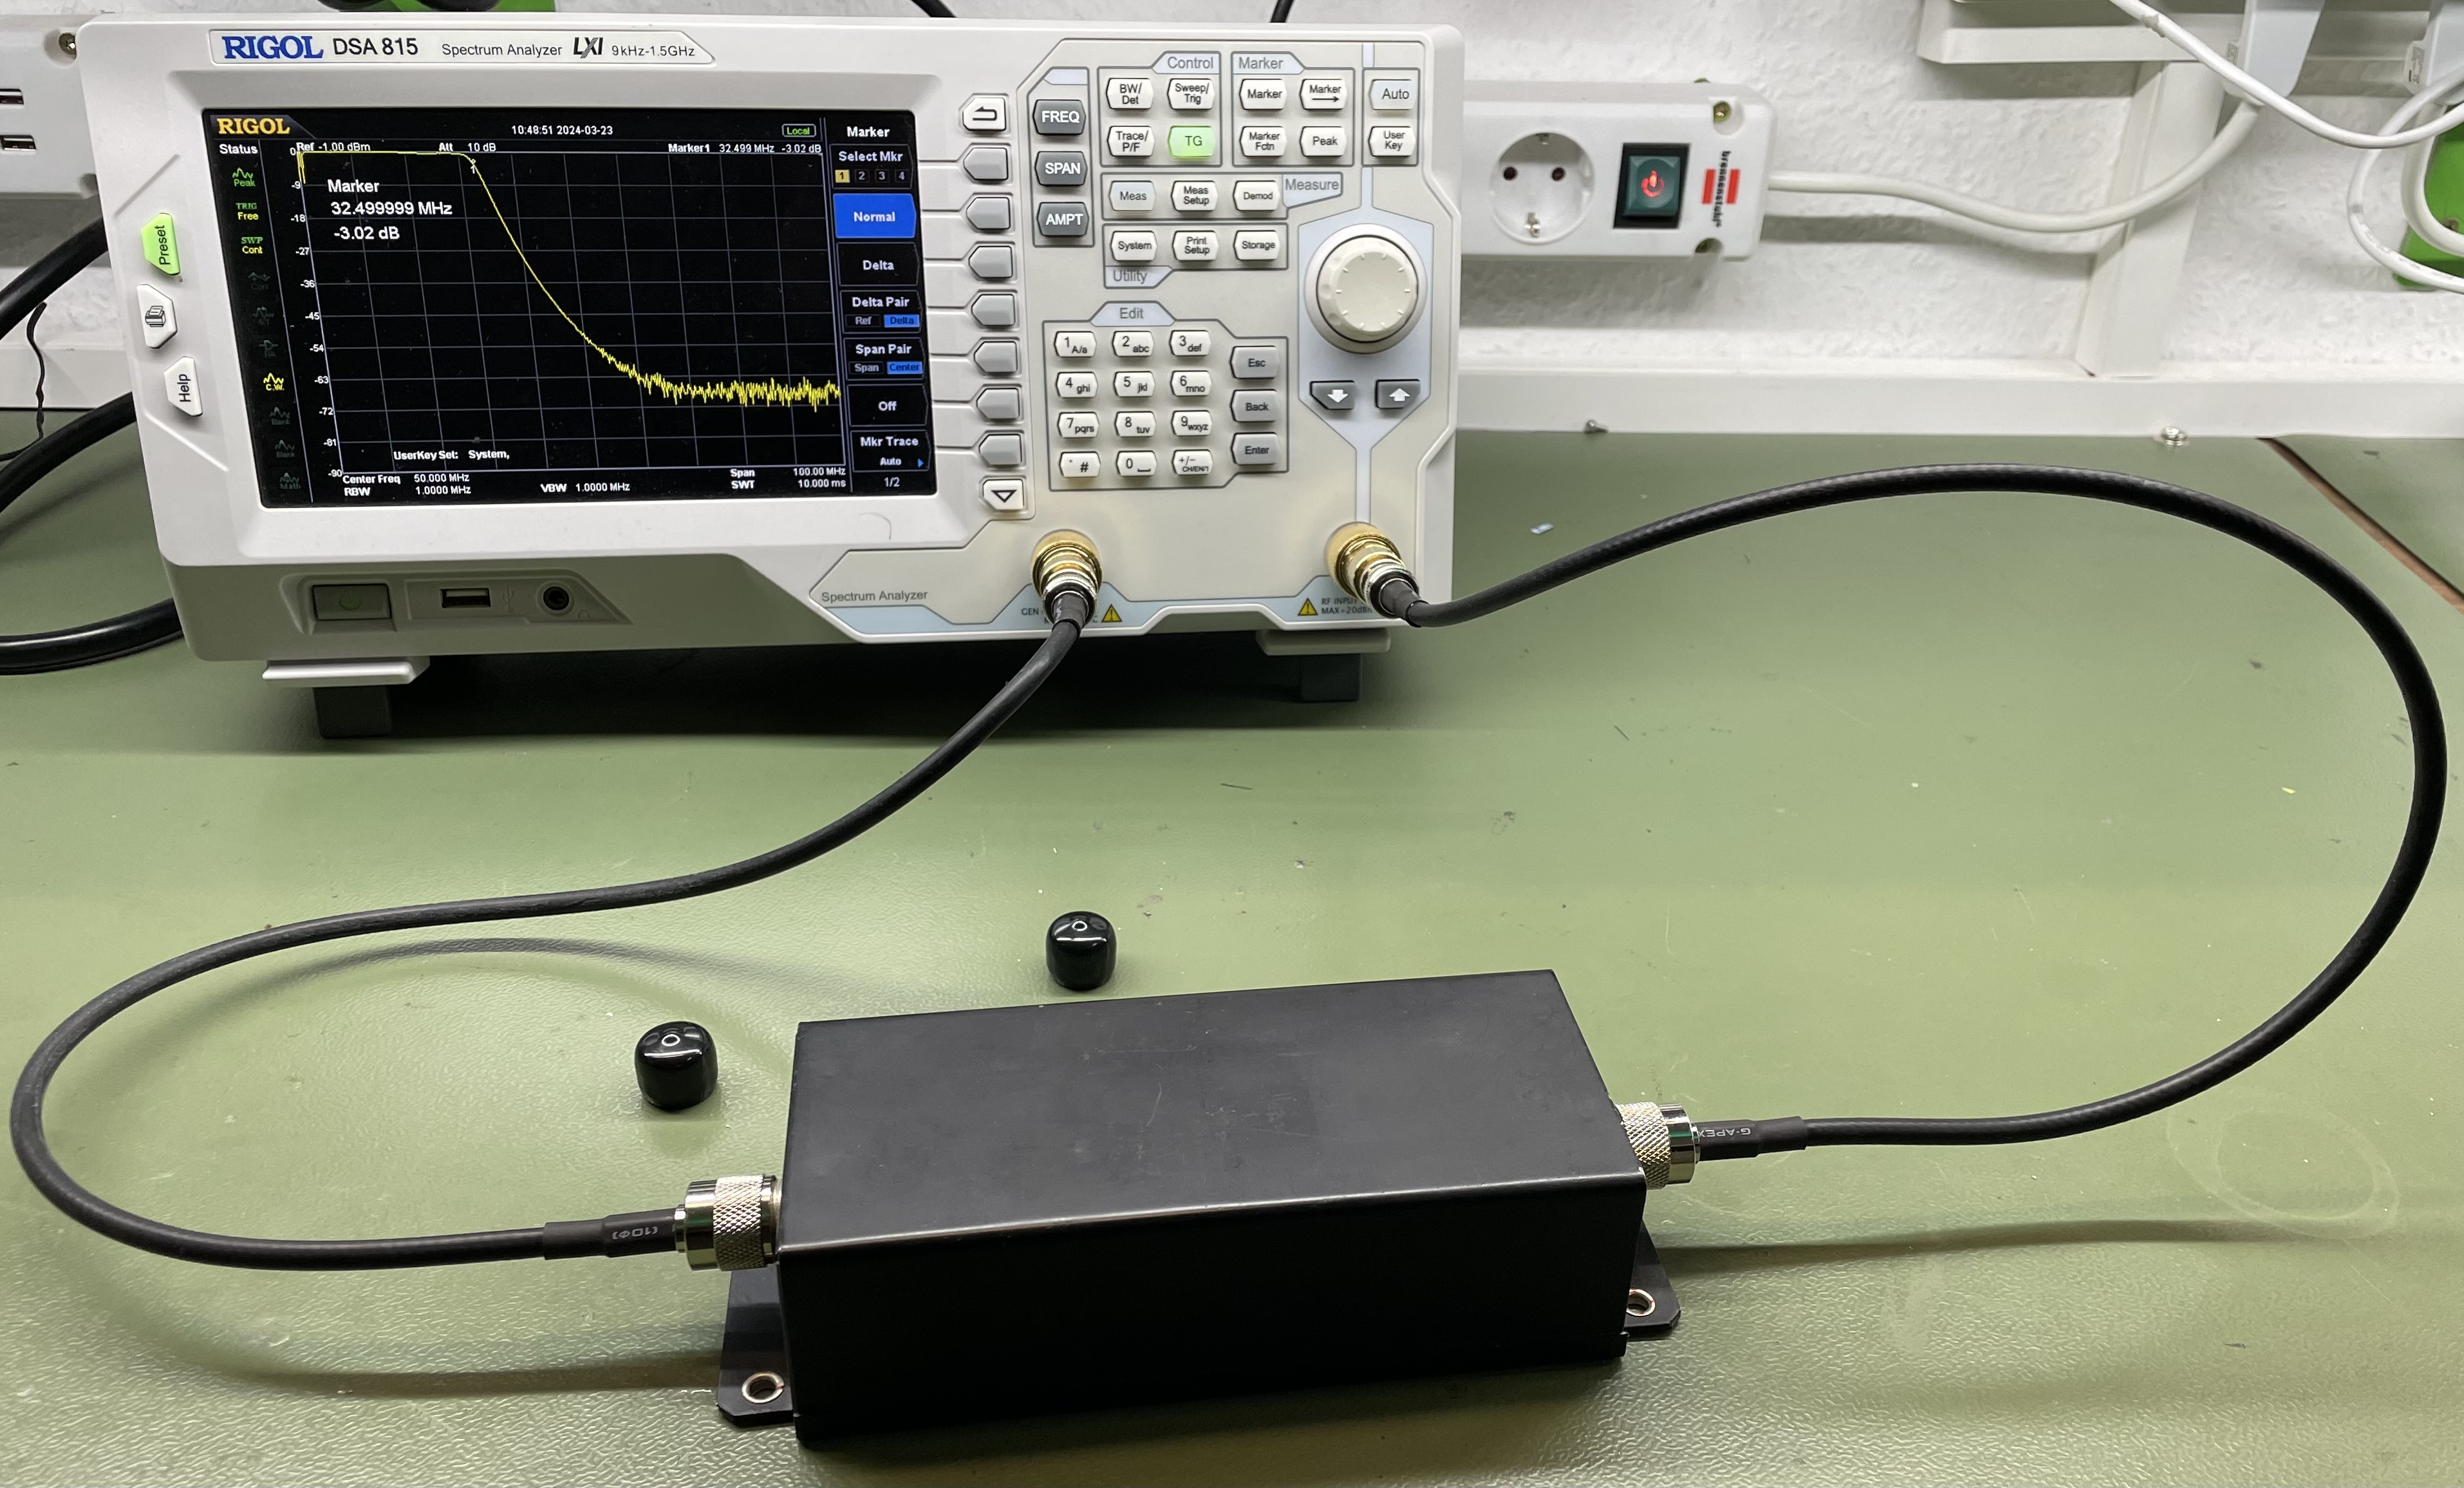
\includegraphics[width=0.85\textwidth]{foto/201}
    \caption{\scriptsize Messung eines Tiefpassfilters mit Grenzfrequenz bei 30MHz}
    \label{e_vna_tiefpassmessung}
\end{figure}

   \end{column}
\end{columns}

\end{frame}

\begin{frame}
\only<1>{
\begin{QQuestion}{EI201}{Wozu wird ein \glqq vektorieller Netzwerkanalysator\grqq{} (VNA) beispielsweise verwendet?}{Zur Bestimmung des Erdungswiderstandes einer Amateurfunkstation.}
{Zum Aufzeichnen des zeitlichen Verlaufs schneller Wechselströme.}
{Zur Überprüfung der Frequenzreinheit eines Senders.}
{Zur genaueren Bestimmung von Resonanzfrequenzen und Impedanzen von Schwingkreisen und Antennen.}
\end{QQuestion}

}
\only<2>{
\begin{QQuestion}{EI201}{Wozu wird ein \glqq vektorieller Netzwerkanalysator\grqq{} (VNA) beispielsweise verwendet?}{Zur Bestimmung des Erdungswiderstandes einer Amateurfunkstation.}
{Zum Aufzeichnen des zeitlichen Verlaufs schneller Wechselströme.}
{Zur Überprüfung der Frequenzreinheit eines Senders.}
{\textbf{\textcolor{DARCgreen}{Zur genaueren Bestimmung von Resonanzfrequenzen und Impedanzen von Schwingkreisen und Antennen.}}}
\end{QQuestion}

}
\end{frame}

\begin{frame}
\only<1>{
\begin{QQuestion}{EI202}{Wie ermittelt man die Resonanzfrequenz eines Schwingkreises? Man ermittelt sie~...}{durch Messung von $L$ und $C$ und Berechnung oder z.~B. mit einem vektoriellen Netzwerkanalysator (VNA).}
{mit einem Frequenzmesser oder einem Oszilloskop.}
{mit einem Digital-Multimeter in der Stellung Frequenzmessung.}
{mit Hilfe der S-Meter-Anzeige bei Anschluss des Schwingkreises an den Empfängereingang.}
\end{QQuestion}

}
\only<2>{
\begin{QQuestion}{EI202}{Wie ermittelt man die Resonanzfrequenz eines Schwingkreises? Man ermittelt sie~...}{\textbf{\textcolor{DARCgreen}{durch Messung von $L$ und $C$ und Berechnung oder z.~B. mit einem vektoriellen Netzwerkanalysator (VNA).}}}
{mit einem Frequenzmesser oder einem Oszilloskop.}
{mit einem Digital-Multimeter in der Stellung Frequenzmessung.}
{mit Hilfe der S-Meter-Anzeige bei Anschluss des Schwingkreises an den Empfängereingang.}
\end{QQuestion}

}
\end{frame}

\begin{frame}
\only<1>{
\begin{QQuestion}{EI203}{Mit welchem Messgerät können Impedanzen, Blindwiderstände und Stehwellenverhältnisse direkt gemessen werden?}{digitales Speicheroszilloskop}
{analoges Multimeter}
{vektorieller Netzwerkanalysator}
{True RMS-Voltmeter}
\end{QQuestion}

}
\only<2>{
\begin{QQuestion}{EI203}{Mit welchem Messgerät können Impedanzen, Blindwiderstände und Stehwellenverhältnisse direkt gemessen werden?}{digitales Speicheroszilloskop}
{analoges Multimeter}
{\textbf{\textcolor{DARCgreen}{vektorieller Netzwerkanalysator}}}
{True RMS-Voltmeter}
\end{QQuestion}

}
\end{frame}

\begin{frame}
\only<1>{
\begin{QQuestion}{EI204}{Wozu ist ein vektorieller Netzwerkanalysator (VNA) beispielsweise geeignet?}{Datenübertragungsraten in Netzwerken erfassen.}
{Messen von Impedanzen.}
{Direkte Messung der Sendeleistung.}
{Messen von Oberschwingungen.}
\end{QQuestion}

}
\only<2>{
\begin{QQuestion}{EI204}{Wozu ist ein vektorieller Netzwerkanalysator (VNA) beispielsweise geeignet?}{Datenübertragungsraten in Netzwerken erfassen.}
{\textbf{\textcolor{DARCgreen}{Messen von Impedanzen.}}}
{Direkte Messung der Sendeleistung.}
{Messen von Oberschwingungen.}
\end{QQuestion}

}
\end{frame}

\begin{frame}
\frametitle{Kalibrierung}
\begin{itemize}
  \item Vor der Benutzung kalibrieren
  \item Zustand \emph{offen}: unendlicher Widerstand
  \item Zustand \emph{Kurzschluss}: Widerstand nahe Null
  \item Zustand \emph{angepasst}: z.B. mit 50 Ω Widerstand sollte ein SWR von 1 angezeigt werden
  \end{itemize}
\end{frame}

\begin{frame}
\only<1>{
\begin{QQuestion}{EI205}{Welche Maßnahme ist vor Gebrauch eines vektoriellen Netzwerkanalysators (VNA) zusammen mit dem Messaufbau durchzuführen?}{Rauschunterdrückung aktivieren}
{Nullpunktabgleich}
{Einstellen der Triggerschwelle}
{Kalibrierung}
\end{QQuestion}

}
\only<2>{
\begin{QQuestion}{EI205}{Welche Maßnahme ist vor Gebrauch eines vektoriellen Netzwerkanalysators (VNA) zusammen mit dem Messaufbau durchzuführen?}{Rauschunterdrückung aktivieren}
{Nullpunktabgleich}
{Einstellen der Triggerschwelle}
{\textbf{\textcolor{DARCgreen}{Kalibrierung}}}
\end{QQuestion}

}
\end{frame}

\begin{frame}
\only<1>{
\begin{QQuestion}{EI206}{Sie ermitteln die Resonanzfrequenz und die Impedanz ihrer selbstgebauten Antennen mit Hilfe eines vektoriellen Netzwerkanalysators (VNA). Wie könnten Sie die Funktion des Gerätes vorher prüfen?}{Durch Beschalten des Messeingangs am VNA mit einem Abschlusswiderstand. Das angezeigte SWR sollte im gesamten Frequenzbereich größer als 2 sein.}
{Durch Prüfen der Anzeigewerte in den Betriebszuständen Leerlauf und Anpassung. Der Messanschluss des Gerätes darf keinesfalls kurzgeschlossen werden.}
{Durch Prüfen der Anzeigewerte in den Betriebszuständen Kurzschluss, Leerlauf und Anpassung. Das SWR sollte bei Anpassung nahe bei 1, bei Kurzschluss und Leerlauf unendlich sein.}
{Durch Beschalten des Messeingangs am VNA mit einem Blindwiderstand. Der Anzeigewert des SWR muss bei allen Frequenzen nahe bei 1 sein.}
\end{QQuestion}

}
\only<2>{
\begin{QQuestion}{EI206}{Sie ermitteln die Resonanzfrequenz und die Impedanz ihrer selbstgebauten Antennen mit Hilfe eines vektoriellen Netzwerkanalysators (VNA). Wie könnten Sie die Funktion des Gerätes vorher prüfen?}{Durch Beschalten des Messeingangs am VNA mit einem Abschlusswiderstand. Das angezeigte SWR sollte im gesamten Frequenzbereich größer als 2 sein.}
{Durch Prüfen der Anzeigewerte in den Betriebszuständen Leerlauf und Anpassung. Der Messanschluss des Gerätes darf keinesfalls kurzgeschlossen werden.}
{\textbf{\textcolor{DARCgreen}{Durch Prüfen der Anzeigewerte in den Betriebszuständen Kurzschluss, Leerlauf und Anpassung. Das SWR sollte bei Anpassung nahe bei 1, bei Kurzschluss und Leerlauf unendlich sein.}}}
{Durch Beschalten des Messeingangs am VNA mit einem Blindwiderstand. Der Anzeigewert des SWR muss bei allen Frequenzen nahe bei 1 sein.}
\end{QQuestion}

}
\end{frame}%ENDCONTENT


\section{Mantelwellen I}
\label{section:mantelwellen_1}
\begin{frame}%STARTCONTENT
\begin{itemize}
  \item Ziel beim Aufbau einer Funkanlage: Nur die Antenne soll Signale abstrahlen bzw. aufnehmen
  \item Dazu eignen sich geschirmte Leitungen, z.B. Koaxialkabel
  \item Im Idealfall strahlen sie selbst nicht oder nehmen keine Strahlung auf
  \end{itemize}
\end{frame}

\begin{frame}
\begin{columns}
    \begin{column}{0.48\textwidth}
    \begin{itemize}
  \item Unsymmetrisches Koaxialkabel wird an symmetrischen Dipol angeschlossen
  \item Auf der Außenseite des Koaxialkabels können hochfrequente Ströme fließen
  \item Dadurch strahlt das Kabel selbst $\rightarrow$ \emph{Mantelwellen}
  \item Mantelströme fehlen, was zur Verformung der Richtcharakteristik führt
  \end{itemize}

    \end{column}
   \begin{column}{0.48\textwidth}
       
\begin{figure}
    \DARCimage{0.85\linewidth}{633include}
    \caption{\scriptsize Mantelstrom bei I<sub>3</sub>}
    \label{e_mantelwelle_effekt}
\end{figure}


   \end{column}
\end{columns}

\end{frame}

\begin{frame}
\only<1>{
\begin{QQuestion}{EG405}{Mantelwellen auf dem Koaxialkabel zur Antenne~...}{werden durch Fehlanpassung und Überlastung des Transceivers verursacht.}
{sind für die Funktionsweise jeder koaxial-gespeisten Antenne notwendig.}
{können zu Störungen anderer Geräte und Störungen des eigenen Empfangs führen.}
{werden für die Messung des Stromes beim SWR verwendet.}
\end{QQuestion}

}
\only<2>{
\begin{QQuestion}{EG405}{Mantelwellen auf dem Koaxialkabel zur Antenne~...}{werden durch Fehlanpassung und Überlastung des Transceivers verursacht.}
{sind für die Funktionsweise jeder koaxial-gespeisten Antenne notwendig.}
{\textbf{\textcolor{DARCgreen}{können zu Störungen anderer Geräte und Störungen des eigenen Empfangs führen.}}}
{werden für die Messung des Stromes beim SWR verwendet.}
\end{QQuestion}

}
\end{frame}

\begin{frame}
\only<1>{
\begin{QQuestion}{EG406}{Welche Effekte treten auf, wenn ein Halbwellendipol mit einem Koaxkabel gleicher Impedanz mittig gespeist wird?}{Es treten Polarisationsdrehungen auf, die von der Kabellänge abhängig sind.}
{Es treten keine nennenswerten Effekte auf, da die Antenne angepasst ist und die Speisung über ein Koaxkabel erfolgt, dessen Außenleiter Erdpotential hat.}
{Am Speisepunkt der Antenne treten gegenphasige Spannungen und Ströme gleicher Größe auf, die eine Fehlanpassung hervorrufen.}
{Die Richtcharakteristik der Antenne wird verformt und es treten Mantelwellen auf.}
\end{QQuestion}

}
\only<2>{
\begin{QQuestion}{EG406}{Welche Effekte treten auf, wenn ein Halbwellendipol mit einem Koaxkabel gleicher Impedanz mittig gespeist wird?}{Es treten Polarisationsdrehungen auf, die von der Kabellänge abhängig sind.}
{Es treten keine nennenswerten Effekte auf, da die Antenne angepasst ist und die Speisung über ein Koaxkabel erfolgt, dessen Außenleiter Erdpotential hat.}
{Am Speisepunkt der Antenne treten gegenphasige Spannungen und Ströme gleicher Größe auf, die eine Fehlanpassung hervorrufen.}
{\textbf{\textcolor{DARCgreen}{Die Richtcharakteristik der Antenne wird verformt und es treten Mantelwellen auf.}}}
\end{QQuestion}

}
\end{frame}

\begin{frame}
\only<1>{
\begin{PQuestion}{EG404}{Die Darstellung zeigt die bei Ankopplung eines Koaxialkabels an eine Antenne auftretenden Ströme. Wie wird der mit $I_3$ bezeichnete Strom genannt?}{Mantelstrom}
{Rückwärtsstrom}
{Potentialstrom}
{Phantomstrom}
{\DARCimage{1.0\linewidth}{633include}}\end{PQuestion}

}
\only<2>{
\begin{PQuestion}{EG404}{Die Darstellung zeigt die bei Ankopplung eines Koaxialkabels an eine Antenne auftretenden Ströme. Wie wird der mit $I_3$ bezeichnete Strom genannt?}{\textbf{\textcolor{DARCgreen}{Mantelstrom}}}
{Rückwärtsstrom}
{Potentialstrom}
{Phantomstrom}
{\DARCimage{1.0\linewidth}{633include}}\end{PQuestion}

}
\end{frame}

\begin{frame}
\frametitle{Mantelwellen verhindern}
\begin{itemize}
  \item Durch ein \emph{Symmetrierglied}, einen Balun (balanced-unbalanced)
  \item Oder zur Dämpfung Koaxialkabel auf einen Ferritkern wickeln
  \end{itemize}
\end{frame}

\begin{frame}
\only<1>{
\begin{QQuestion}{EG407}{Wozu wird ein Symmetrierglied (Balun) beispielsweise verwendet?}{Zur Nutzung einer Wechselspannungsversorgung am Gleichstromanschluss eines Transceivers}
{Zur Einstellung der Frequenzablage für Relaisbetrieb}
{Zum Anschluss eines Koaxialkabels an eine Dipol-Antenne}
{Zur Umschaltung zwischen horizontaler und vertikaler Polarisation einer Kreuz-Yagi-Uda}
\end{QQuestion}

}
\only<2>{
\begin{QQuestion}{EG407}{Wozu wird ein Symmetrierglied (Balun) beispielsweise verwendet?}{Zur Nutzung einer Wechselspannungsversorgung am Gleichstromanschluss eines Transceivers}
{Zur Einstellung der Frequenzablage für Relaisbetrieb}
{\textbf{\textcolor{DARCgreen}{Zum Anschluss eines Koaxialkabels an eine Dipol-Antenne}}}
{Zur Umschaltung zwischen horizontaler und vertikaler Polarisation einer Kreuz-Yagi-Uda}
\end{QQuestion}

}
\end{frame}

\begin{frame}
\only<1>{
\begin{PQuestion}{EG408}{Auf einem Ferritkern sind einige Windungen Koaxialkabel aufgewickelt. Mit diesem Aufbau~...}{lassen sich Oberwellen unterdrücken.}
{lassen sich statische Aufladungen verhindern.}
{lässt sich die Trennschärfe verbessern.}
{lassen sich Mantelwellen dämpfen.}
{\DARCimage{0.5\linewidth}{40include}}\end{PQuestion}

}
\only<2>{
\begin{PQuestion}{EG408}{Auf einem Ferritkern sind einige Windungen Koaxialkabel aufgewickelt. Mit diesem Aufbau~...}{lassen sich Oberwellen unterdrücken.}
{lassen sich statische Aufladungen verhindern.}
{lässt sich die Trennschärfe verbessern.}
{\textbf{\textcolor{DARCgreen}{lassen sich Mantelwellen dämpfen.}}}
{\DARCimage{0.5\linewidth}{40include}}\end{PQuestion}

}
\end{frame}%ENDCONTENT


\title{DARC Amateurfunklehrgang Klasse E}
\author{Personenschutzabstand}
\institute{Deutscher Amateur Radio Club e.\,V.}
\begin{frame}
\maketitle
\end{frame}

\section{Äquivalente isotrope Strahlungsleistung (EIRP) II}
\label{section:aequivalente_isotrope_strahlungsleistung_eirp_2}
\begin{frame}%STARTCONTENT
\begin{itemize}
  \item Bei der Berechnung nur die Energie berücksichtigen, die an der Antenne ankommt
  \item Verluste $a$ durch Kabel, Stecker oder andere Bauteile abziehen
  \item Erst dann mit dem Gewinnfaktor multiplizieren
  \item Es folgen diverse allgemeine Formeln für ERP und EIRP
  \end{itemize}
\end{frame}

\begin{frame}
\frametitle{ERP}
Aus Klasse~N bekannt:

$P_{\mathrm{ERP}} = (P_{\mathrm{Sender}} -- P_{\mathrm{Verluste}}) \cdot G_{\mathrm{Antenne}}$
    \pause
    Bei der Rechnung mit dB zu verwenden:

$P_{\mathrm{ERP}} = P_{\mathrm{Sender}} -- a + g_d$
    \pause
    Aus der Formelsammlung mit Umwandlung von dB in Leistungsfaktor:

$P_{\mathrm{ERP}} = P_{\mathrm{Sender}} \cdot 10^{\frac{g_d -- a}{10\mathrm{dB}}}$



\end{frame}

\begin{frame}
\frametitle{EIRP}
Umrechnung ERP zu EIRP:

$P_{\mathrm{EIRP}} = P_{\mathrm{ERP}} + 2,15 \mathrm{dB}$
    \pause
    Aus der Formelsammlung mit Umwandlung von dB in Leistungsfaktor:

$P_{\mathrm{EIRP}} = P_{\mathrm{Sender}} \cdot 10^{\frac{g_d -- a + 2,15\mathrm{dB}}{10\mathrm{dB}}}$
    \pause
    Wenn der Gewinn in dBi angegeben ist:

$P_{\mathrm{EIRP}} = P_{\mathrm{Sender}} \cdot 10^{\frac{g_i -- a}{10\mathrm{dB}}}$



\end{frame}

\begin{frame}
\only<1>{
\begin{QQuestion}{EG501}{Die äquivalente isotrope Strahlungsleistung (EIRP) ist~...}{die durchschnittliche Leistung bei der höchsten Spitze der Modulationshüllkurve, die der Antenne zugeführt wird, und ihrem Gewinn in einer Richtung, bezogen auf den isotropen Strahler.}
{das Produkt aus der Leistung, die unmittelbar der Antenne zugeführt wird, und ihrem Gewinn in einer Richtung, bezogen auf den Dipol.}
{das Produkt aus der Leistung, die unmittelbar der Antenne zugeführt wird, und ihrem Gewinn in einer Richtung, bezogen auf den isotropen Strahler.}
{die durchschnittliche Leistung bei der höchsten Spitze der Modulationshüllkurve, die der Antenne zugeführt wird, und ihrem Gewinn in einer Richtung, bezogen auf den Dipol.}
\end{QQuestion}

}
\only<2>{
\begin{QQuestion}{EG501}{Die äquivalente isotrope Strahlungsleistung (EIRP) ist~...}{die durchschnittliche Leistung bei der höchsten Spitze der Modulationshüllkurve, die der Antenne zugeführt wird, und ihrem Gewinn in einer Richtung, bezogen auf den isotropen Strahler.}
{das Produkt aus der Leistung, die unmittelbar der Antenne zugeführt wird, und ihrem Gewinn in einer Richtung, bezogen auf den Dipol.}
{\textbf{\textcolor{DARCgreen}{das Produkt aus der Leistung, die unmittelbar der Antenne zugeführt wird, und ihrem Gewinn in einer Richtung, bezogen auf den isotropen Strahler.}}}
{die durchschnittliche Leistung bei der höchsten Spitze der Modulationshüllkurve, die der Antenne zugeführt wird, und ihrem Gewinn in einer Richtung, bezogen auf den Dipol.}
\end{QQuestion}

}
\end{frame}

\begin{frame}
\only<1>{
\begin{QQuestion}{EG502}{Nach welcher der Antworten kann die EIRP berechnet werden?}{$P_{\symup{EIRP}} = (P_{\symup{Sender}} - P_{\symup{Verluste}}) \cdot G_{\symup{Antenne}}$, bezogen auf einen isotropen Strahler}
{$P_{\symup{EIRP}} = (P_{\symup{Sender}} \cdot P_{\symup{Verluste}}) \cdot G_{\symup{Antenne}}$, bezogen auf einen Halbwellendipol}
{$P_{\symup{EIRP}} = (P_{\symup{Sender}} - P_{\symup{Verluste}}) + G_{\symup{Antenne}}$, bezogen auf einen isotropen Strahler}
{$P_{\symup{EIRP}} = (P_{\symup{Sender}} - P_{\symup{Verluste}}) + G_{\symup{Antenne}}$, bezogen auf einen Halbwellendipol}
\end{QQuestion}

}
\only<2>{
\begin{QQuestion}{EG502}{Nach welcher der Antworten kann die EIRP berechnet werden?}{\textbf{\textcolor{DARCgreen}{$P_{\symup{EIRP}} = (P_{\symup{Sender}} - P_{\symup{Verluste}}) \cdot G_{\symup{Antenne}}$, bezogen auf einen isotropen Strahler}}}
{$P_{\symup{EIRP}} = (P_{\symup{Sender}} \cdot P_{\symup{Verluste}}) \cdot G_{\symup{Antenne}}$, bezogen auf einen Halbwellendipol}
{$P_{\symup{EIRP}} = (P_{\symup{Sender}} - P_{\symup{Verluste}}) + G_{\symup{Antenne}}$, bezogen auf einen isotropen Strahler}
{$P_{\symup{EIRP}} = (P_{\symup{Sender}} - P_{\symup{Verluste}}) + G_{\symup{Antenne}}$, bezogen auf einen Halbwellendipol}
\end{QQuestion}

}
\end{frame}

\begin{frame}
\frametitle{Ortsfeste Amateurfunkanlage}
Eine ortsfeste Amateurfunkanlage ist nach §~9 BEMFV bei der BNetzA anzuzeigen, wenn eine Strahlungsleistung von \qty{10}{\watt} EIRP überschritten wird.

\end{frame}

\begin{frame}
\only<1>{
\begin{QQuestion}{EG503}{Ein HF-Verstärker für \qty{5,7}{\GHz} speist eine Ausgangsleistung von \qty{250}{\mW} ohne Leitungsverluste direkt in einen Parabolspiegel mit einem Gewinn von \qty{26}{\dBi} ein. Wie hoch ist die äquivalente Strahlungsleistung (EIRP)?}{\qty{100}{\W}}
{\qty{61}{\W}}
{\qty{6,5}{\W}}
{\qty{3,4}{\W}}
\end{QQuestion}

}
\only<2>{
\begin{QQuestion}{EG503}{Ein HF-Verstärker für \qty{5,7}{\GHz} speist eine Ausgangsleistung von \qty{250}{\mW} ohne Leitungsverluste direkt in einen Parabolspiegel mit einem Gewinn von \qty{26}{\dBi} ein. Wie hoch ist die äquivalente Strahlungsleistung (EIRP)?}{\textbf{\textcolor{DARCgreen}{\qty{100}{\W}}}}
{\qty{61}{\W}}
{\qty{6,5}{\W}}
{\qty{3,4}{\W}}
\end{QQuestion}

}
\end{frame}

\begin{frame}
\frametitle{Lösungsweg}
\begin{itemize}
  \item gegeben: $P_{\mathrm{Sender}} = 250mW$
  \item gegeben: $g_i = 26\mathrm{dB}$
  \item gegeben: $a = 0$
  \item gesucht: $P_{\mathrm{EIRP}}$
  \end{itemize}
    \pause
    \begin{equation}\begin{split} \nonumber P_{\mathrm{EIRP}} &= P_{\mathrm{Sender}} \cdot 10^{\frac{g_i -- a}{10\mathrm{dB}}}\\ &= 250mW \cdot 10^{\frac{26\mathrm{dB}}{10\mathrm{dB}}}\\ &= 250mW \cdot 398\\ &\approx 100W \end{split}\end{equation}



\end{frame}

\begin{frame}
\only<1>{
\begin{QQuestion}{EG504}{Ein HF-Verstärker für \qty{10,4}{\GHz} speist eine Ausgangsleistung von \qty{5}{\W} direkt in einen Parabolspiegel mit einem Gewinn von \qty{36}{\dBi} ein. Wie hoch ist die äquivalente Strahlungsleistung (EIRP)?}{\qty{180}{\W}}
{\qty{12195}{\W}}
{\qty{20000}{\W}}
{\qty{110}{\W}}
\end{QQuestion}

}
\only<2>{
\begin{QQuestion}{EG504}{Ein HF-Verstärker für \qty{10,4}{\GHz} speist eine Ausgangsleistung von \qty{5}{\W} direkt in einen Parabolspiegel mit einem Gewinn von \qty{36}{\dBi} ein. Wie hoch ist die äquivalente Strahlungsleistung (EIRP)?}{\qty{180}{\W}}
{\qty{12195}{\W}}
{\textbf{\textcolor{DARCgreen}{\qty{20000}{\W}}}}
{\qty{110}{\W}}
\end{QQuestion}

}

\end{frame}

\begin{frame}
\only<1>{
\begin{QQuestion}{EG511}{Sie möchten für Ihre Sendeanlage keine Anzeige einer ortsfesten Amateurfunkanlage nach \S~9~BEMFV abgeben. Wie hoch darf die Sendeleistung für ihre Vertikalantenne mit \qty{5,15}{\dBi} Gewinn ohne Berücksichtigung der Kabelverluste maximal sein, damit die Strahlungsleistung von \qty{10}{\W} EIRP nicht überschritten wird?}{\qty{3}{\W}}
{\qty{10}{\W}}
{\qty{5}{\W}}
{\qty{2}{\W}}
\end{QQuestion}

}
\only<2>{
\begin{QQuestion}{EG511}{Sie möchten für Ihre Sendeanlage keine Anzeige einer ortsfesten Amateurfunkanlage nach \S~9~BEMFV abgeben. Wie hoch darf die Sendeleistung für ihre Vertikalantenne mit \qty{5,15}{\dBi} Gewinn ohne Berücksichtigung der Kabelverluste maximal sein, damit die Strahlungsleistung von \qty{10}{\W} EIRP nicht überschritten wird?}{\textbf{\textcolor{DARCgreen}{\qty{3}{\W}}}}
{\qty{10}{\W}}
{\qty{5}{\W}}
{\qty{2}{\W}}
\end{QQuestion}

}
\end{frame}

\begin{frame}
\frametitle{Lösungsweg}
\begin{itemize}
  \item gegeben: $P_{\mathrm{EIRP}} = 10W$
  \item gegeben: $g_i = 5,15\mathrm{dB}$
  \item gegeben: $a = 0$
  \item gesucht: $P_{\mathrm{Sender}}$
  \end{itemize}
    \pause
    \begin{equation}\begin{split} \nonumber P_{\mathrm{EIRP}} &= P_{\mathrm{Sender}} \cdot 10^{\frac{g_i -- a}{10\mathrm{dB}}}\\ \Rightarrow P_{\mathrm{Sender}} &= \dfrac{P_{\mathrm{EIRP}}}{10^{\frac{g_i -- a}{10\mathrm{dB}}}}\\ &= \dfrac{10W}{10^{\frac{5,15\mathrm{dB}}{10\mathrm{dB}}}}\\ &\approx \frac{10W}{3,27} \approx 3W \end{split}\end{equation}

\end{frame}

\begin{frame}
\only<1>{
\begin{QQuestion}{EG505}{An einen Sender mit \qty{100}{\W} Ausgangsleistung ist eine Antenne mit einem Gewinn von \qty{11}{\dBi} angeschlossen. Die Dämpfung des Kabels beträgt \qty{1}{\decibel}. Wie hoch ist die äquivalente Strahlungsleistung (EIRP)?}{\qty{164}{\W}}
{\qty{1000}{\W}}
{\qty{100}{\W}}
{\qty{1640}{\W}}
\end{QQuestion}

}
\only<2>{
\begin{QQuestion}{EG505}{An einen Sender mit \qty{100}{\W} Ausgangsleistung ist eine Antenne mit einem Gewinn von \qty{11}{\dBi} angeschlossen. Die Dämpfung des Kabels beträgt \qty{1}{\decibel}. Wie hoch ist die äquivalente Strahlungsleistung (EIRP)?}{\qty{164}{\W}}
{\textbf{\textcolor{DARCgreen}{\qty{1000}{\W}}}}
{\qty{100}{\W}}
{\qty{1640}{\W}}
\end{QQuestion}

}

\end{frame}

\begin{frame}
\only<1>{
\begin{QQuestion}{EG507}{An einen Sender mit \qty{100}{\W} Ausgangsleistung ist eine Dipol-Antenne angeschlossen. Die Dämpfung des Kabels beträgt \qty{10}{\decibel}. Wie hoch ist die äquivalente isotrope Strahlungsleistung (EIRP)?}{\qty{16,4}{\W}}
{\qty{90}{\W}}
{\qty{164}{\W}}
{\qty{10}{\W}}
\end{QQuestion}

}
\only<2>{
\begin{QQuestion}{EG507}{An einen Sender mit \qty{100}{\W} Ausgangsleistung ist eine Dipol-Antenne angeschlossen. Die Dämpfung des Kabels beträgt \qty{10}{\decibel}. Wie hoch ist die äquivalente isotrope Strahlungsleistung (EIRP)?}{\textbf{\textcolor{DARCgreen}{\qty{16,4}{\W}}}}
{\qty{90}{\W}}
{\qty{164}{\W}}
{\qty{10}{\W}}
\end{QQuestion}

}

\end{frame}

\begin{frame}
\only<1>{
\begin{QQuestion}{EG506}{Ein Sender mit \qty{75}{\W} Ausgangsleistung ist über eine Antennenleitung, die \qty{2,15}{\decibel} (Faktor $1,64$) Kabelverluste hat, an eine Dipol-Antenne angeschlossen. Welche EIRP wird von der Antenne maximal abgestrahlt?}{\qty{75}{\W}}
{\qty{123}{\W}}
{\qty{45,7}{\W}}
{\qty{60,6}{\W}}
\end{QQuestion}

}
\only<2>{
\begin{QQuestion}{EG506}{Ein Sender mit \qty{75}{\W} Ausgangsleistung ist über eine Antennenleitung, die \qty{2,15}{\decibel} (Faktor $1,64$) Kabelverluste hat, an eine Dipol-Antenne angeschlossen. Welche EIRP wird von der Antenne maximal abgestrahlt?}{\textbf{\textcolor{DARCgreen}{\qty{75}{\W}}}}
{\qty{123}{\W}}
{\qty{45,7}{\W}}
{\qty{60,6}{\W}}
\end{QQuestion}

}

\end{frame}

\begin{frame}\begin{itemize}
  \item Ist der Antennengewinn bezogen auf den Dipol angegeben, müssen wir den Gewinn des Dipols noch zusätzlich berücksichtigen, wenn nach der EIRP gefragt ist.
  \end{itemize}
\end{frame}

\begin{frame}
\only<1>{
\begin{QQuestion}{EG508}{Ein Sender mit \qty{5}{\W} Ausgangsleistung ist über eine Antennenleitung, die \qty{2}{\decibel} Kabelverluste hat, an eine Richtantenne mit \qty{5}{\decibel} Gewinn (auf den Dipol bezogen) angeschlossen. Welche EIRP wird von der Antenne abgestrahlt?}{\qty{9,98}{\W}}
{\qty{8,2}{\W}}
{\qty{41,2}{\W}}
{\qty{16,4}{\W}}
\end{QQuestion}

}
\only<2>{
\begin{QQuestion}{EG508}{Ein Sender mit \qty{5}{\W} Ausgangsleistung ist über eine Antennenleitung, die \qty{2}{\decibel} Kabelverluste hat, an eine Richtantenne mit \qty{5}{\decibel} Gewinn (auf den Dipol bezogen) angeschlossen. Welche EIRP wird von der Antenne abgestrahlt?}{\qty{9,98}{\W}}
{\qty{8,2}{\W}}
{\qty{41,2}{\W}}
{\textbf{\textcolor{DARCgreen}{\qty{16,4}{\W}}}}
\end{QQuestion}

}
\end{frame}

\begin{frame}
\frametitle{Lösungsweg}
\begin{itemize}
  \item gegeben: $P_{\mathrm{Sender}} = 5W$
  \item gegeben: $g_d = 5\mathrm{dB}$
  \item gegeben: $a = 2\mathrm{dB}$
  \item gesucht: $P_{\mathrm{EIRP}}$
  \end{itemize}
    \pause
    \begin{equation}\begin{split} \nonumber P_{\mathrm{EIRP}} &= P_{\mathrm{Sender}} \cdot 10^{\frac{g_d -- a + 2,15\mathrm{dB}}{10\mathrm{dB}}}\\ &= 5W \cdot 10^{\frac{5\mathrm{dB} -- 2\mathrm{dB} + 2,15\mathrm{dB}}{10\mathrm{dB}}}\\ &= 5W \cdot 3,27\\ &\approx 16,4W \end{split}\end{equation}



\end{frame}

\begin{frame}
\only<1>{
\begin{QQuestion}{EG509}{Ein Sender mit \qty{0,6}{\W} Ausgangsleistung ist über eine Antennenleitung, die \qty{1}{\decibel} Kabelverluste hat, an eine Richtantenne mit \qty{11}{\decibel}~Gewinn (auf Dipol bezogen) angeschlossen. Welche EIRP wird von der Antenne maximal abgestrahlt?}{\qty{12,7}{\W}}
{\qty{6,0}{\W}}
{\qty{7,8}{\W}}
{\qty{9,8}{\W}}
\end{QQuestion}

}
\only<2>{
\begin{QQuestion}{EG509}{Ein Sender mit \qty{0,6}{\W} Ausgangsleistung ist über eine Antennenleitung, die \qty{1}{\decibel} Kabelverluste hat, an eine Richtantenne mit \qty{11}{\decibel}~Gewinn (auf Dipol bezogen) angeschlossen. Welche EIRP wird von der Antenne maximal abgestrahlt?}{\qty{12,7}{\W}}
{\qty{6,0}{\W}}
{\qty{7,8}{\W}}
{\textbf{\textcolor{DARCgreen}{\qty{9,8}{\W}}}}
\end{QQuestion}

}

\end{frame}

\begin{frame}
\only<1>{
\begin{QQuestion}{EG510}{Ein Sender mit \qty{8,5}{\W} Ausgangsleistung ist über eine Antennenleitung, die \qty{1,5}{\decibel} Kabelverluste hat, an eine Antenne mit \qty{0}{\decibel} Gewinn (auf den Dipol bezogen) angeschlossen. Welche EIRP wird von der Antenne abgestrahlt?}{\qty{9,9}{\W}}
{\qty{19,7}{\W}}
{\qty{12,0}{\W}}
{\qty{6,0}{\W}}
\end{QQuestion}

}
\only<2>{
\begin{QQuestion}{EG510}{Ein Sender mit \qty{8,5}{\W} Ausgangsleistung ist über eine Antennenleitung, die \qty{1,5}{\decibel} Kabelverluste hat, an eine Antenne mit \qty{0}{\decibel} Gewinn (auf den Dipol bezogen) angeschlossen. Welche EIRP wird von der Antenne abgestrahlt?}{\textbf{\textcolor{DARCgreen}{\qty{9,9}{\W}}}}
{\qty{19,7}{\W}}
{\qty{12,0}{\W}}
{\qty{6,0}{\W}}
\end{QQuestion}

}

\end{frame}%ENDCONTENT


\section{Personenschutzabstand II}
\label{section:personenschutzabstand_2}
\begin{frame}%STARTCONTENT

\frametitle{Personenschutzgrenzwerte}
\begin{itemize}
  \item Müssen ab einer EIRP von \qty{10}{\watt} nachgewiesen werden
  \item Trotz kleiner Leistung kann es einen hohen Antennengewinn geben
  \item Dann besteht eine Pflicht zur Nachweisführung
  \end{itemize}
\end{frame}

\begin{frame}
\only<1>{
\begin{QQuestion}{EK104}{Muss ein Funkamateur als Betreiber einer ortsfesten Amateurfunkstelle bei FM-Telefonie und einer Sendeleistung von \qty{6}{\W} an einer 15-Element-Yagi-Uda-Antenne mit 13 dBd Gewinn im \qty{2}{\m}-Band die Einhaltung der Personenschutzgrenzwerte nachweisen?}{Ja, er ist in diesem Fall verpflichtet die Einhaltung der Personenschutzgrenzwerte nachzuweisen.}
{Nein, der Schutz von Personen in elektromagnetischen Feldern ist durch den Funkamateur erst bei einer Strahlungsleistung von mehr als \qty{10}{\W} EIRP sicherzustellen.}
{Ja, für ortsfeste Amateurfunkstellen ist die Einhaltung der Personenschutzgrenzwerte in jedem Fall nachzuweisen.}
{Nein, bei FM-Telefonie und Sendezeiten unter 6 Minuten in der Stunde kann der Schutz von Personen in elektromagnetischen Feldern durch den Funkamateur vernachlässigt werden.}
\end{QQuestion}

}
\only<2>{
\begin{QQuestion}{EK104}{Muss ein Funkamateur als Betreiber einer ortsfesten Amateurfunkstelle bei FM-Telefonie und einer Sendeleistung von \qty{6}{\W} an einer 15-Element-Yagi-Uda-Antenne mit 13 dBd Gewinn im \qty{2}{\m}-Band die Einhaltung der Personenschutzgrenzwerte nachweisen?}{\textbf{\textcolor{DARCgreen}{Ja, er ist in diesem Fall verpflichtet die Einhaltung der Personenschutzgrenzwerte nachzuweisen.}}}
{Nein, der Schutz von Personen in elektromagnetischen Feldern ist durch den Funkamateur erst bei einer Strahlungsleistung von mehr als \qty{10}{\W} EIRP sicherzustellen.}
{Ja, für ortsfeste Amateurfunkstellen ist die Einhaltung der Personenschutzgrenzwerte in jedem Fall nachzuweisen.}
{Nein, bei FM-Telefonie und Sendezeiten unter 6 Minuten in der Stunde kann der Schutz von Personen in elektromagnetischen Feldern durch den Funkamateur vernachlässigt werden.}
\end{QQuestion}

}
\end{frame}

\begin{frame}
\frametitle{Sicherheitsabstand}
\begin{itemize}
  \item Bewertungsverfahren nach BEMFV (Verordnung über das Nachweisverfahren zur Begrenzung elektromagnetischer Felder)
  \item Fernfeldberechnung ist für das Fernfeld möglich
  \item Fernfeld bildet sich bei Dipolen in einem Abstand von etwa bei 4λ aus
  \item Bei Berechnung mit der Fernfeldnäherung gilt der Sicherheitsabstand von jedem Punkt der Antenne
  \end{itemize}
\end{frame}

\begin{frame}
\only<1>{
\begin{QQuestion}{EK107}{Sie errechnen einen Sicherheitsabstand für Ihre Antenne. Von welchem Punkt aus muss dieser Sicherheitsabstand eingehalten werden, wenn Sie bei der Berechnung die Fernfeldnäherung verwendet haben? Er muss eingehalten werden~...}{von jedem Punkt der Antenne.}
{vom Einspeisepunkt der Antenne.}
{von der Mitte der Antenne, d.~h. dort, wo sie am Mast befestigt ist.}
{vom untersten Punkt der Antenne.}
\end{QQuestion}

}
\only<2>{
\begin{QQuestion}{EK107}{Sie errechnen einen Sicherheitsabstand für Ihre Antenne. Von welchem Punkt aus muss dieser Sicherheitsabstand eingehalten werden, wenn Sie bei der Berechnung die Fernfeldnäherung verwendet haben? Er muss eingehalten werden~...}{\textbf{\textcolor{DARCgreen}{von jedem Punkt der Antenne.}}}
{vom Einspeisepunkt der Antenne.}
{von der Mitte der Antenne, d.~h. dort, wo sie am Mast befestigt ist.}
{vom untersten Punkt der Antenne.}
\end{QQuestion}

}
\end{frame}%ENDCONTENT


\section{Frequenzabhängigkeit des Personenschutzabstands}
\label{section:personenschutzabstand_frequenzabhaengig}
\begin{frame}%STARTCONTENT
\begin{itemize}
  \item Der menschliche Körper kann hochfrequente Strahlung absorbieren (\textcolor{DARCblue}{\faLink~\href{https://50ohm.de/bfs}{50ohm.de/bfs}})
  \item Die Strahlung wird dabei in Wärme umgewandelt
  \item Thermoregulation des Körpers schafft begrenzt einen Ausgleich
  \end{itemize}
\end{frame}

\begin{frame}
\begin{columns}
    \begin{column}{0.48\textwidth}
    Eindringtiefe der Strahlung:

\begin{itemize}
  \item MHz ca. \qtyrange{10}{30}{\centi\metre}
  \item GHz wenige cm
  \item $>$\qty{10}{\giga\hertz} ca. $<$ \qty{1}{\milli\metre}
  \end{itemize}

    \end{column}
   \begin{column}{0.48\textwidth}
       \begin{itemize}
  \item Resonanz bei $\textrm{Körpergröße} \approx \frac{\lambda}{2}$
  \item Hohe Aufnahme von Strahlungsenergie bei Resonanz
  \item Deshalb sind die \emph{Feldstärkegrenzwerte} für den Schutz von Personen in elektromagnetischen Feldern \emph{von der Frequenz abhängig}
  \end{itemize}

   \end{column}
\end{columns}

\end{frame}

\begin{frame}
\only<1>{
\begin{QQuestion}{EK101}{Die Feldstärkegrenzwerte für den Schutz von Personen in elektromagnetischen Feldern sind von der Frequenz abhängig, weil~...}{auf den Amateurfunkbändern unterschiedlich hohe Sendeleistungen zugelassen sind.}
{niederfrequente elektromagnetische Felder energiereicher sind als hochfrequente.}
{die Fähigkeit des Körpers, hochfrequente Strahlung zu absorbieren, frequenzabhängig ist.}
{die spezifische Absorptionsrate bei einigen Frequenzen nicht messbar ist.}
\end{QQuestion}

}
\only<2>{
\begin{QQuestion}{EK101}{Die Feldstärkegrenzwerte für den Schutz von Personen in elektromagnetischen Feldern sind von der Frequenz abhängig, weil~...}{auf den Amateurfunkbändern unterschiedlich hohe Sendeleistungen zugelassen sind.}
{niederfrequente elektromagnetische Felder energiereicher sind als hochfrequente.}
{\textbf{\textcolor{DARCgreen}{die Fähigkeit des Körpers, hochfrequente Strahlung zu absorbieren, frequenzabhängig ist.}}}
{die spezifische Absorptionsrate bei einigen Frequenzen nicht messbar ist.}
\end{QQuestion}

}
\end{frame}%ENDCONTENT


\section{Zeitbezug beim Personenschutzabstand}
\label{section:personenschutzabstand_zeitbezug}
\begin{frame}%STARTCONTENT

\frametitle{Zeitbezug}
\begin{itemize}
  \item In der \enquote{26. Verordnung zur Durchführung des Bundes-Immissionsschutzgesetzes} wird ein zeitlicher Bezug zur Einhaltung der Feldstärke-Gernzwerte hinzugefügt
  \item Es muss nach drei Fällen für Grenzwerte unterschieden werden
  \end{itemize}
\end{frame}

\begin{frame}
\frametitle{6-Minuten-Intervalle}
\begin{itemize}
  \item Da nicht ständig gesendet wird, Verwendung des quadratischen Mittels der Feldstärke (V/m) über 6 Minuten
  \item Grenzwerte sind frequenzabhängig
  \item z.B. \qty{28}{\volt}/m bei \qty{14}{\mega\hertz}
  \item Berechnung erfolgt mit Näherungsformel (im nächsten Abschnitt)
  \end{itemize}
\end{frame}

\begin{frame}
\frametitle{Momentaner Spitzenwert}
\begin{itemize}
  \item Maximaler momentaner Spitzenwert
  \item Elektrische Feldstärke in kV/m
  \item Grenzwerte sind frequenzabhängig
  \item z.B. \qty{5}{\kilo\volt}/m bei \qty{14}{\mega\hertz}
  \end{itemize}
\end{frame}

\begin{frame}
\frametitle{Gepulste Felder}
\begin{itemize}
  \item Schnelles Ein- und Ausschalten
  \item Als Faktor für den momentanen Spitzenwert oder das 6-Minuten-Intervall
  \item Grenzwerte sind frequenzabhängig
  \item z.B. 32-fache des 6-Minuten-Intervalls bei \qty{14}{\mega\hertz}
  \end{itemize}
\end{frame}

\begin{frame}
\only<1>{
\begin{QQuestion}{EK102}{Mit welchem zeitlichen Bezug ist die Feldstärke für die Einhaltung der Grenzwerte der 26. Verordnung zur Durchführung des Bundes-Immissionsschutzgesetzes (Verordnung über elektromagnetische Felder - 26. BImSchV) zu betrachten?}{Quadratisch gemittelt über 6 Minuten für Grenzwerte nach Anhang 1b, als kurzfristiger Effektivwert für Grenzwerte nach Anhang 1a und als momentaner Spitzenwert für Grenzwerte nach Anhang 3}
{Quadratisch gemittelt über 3 Minuten für Grenzwerte nach Anhang 1b, als kurzfristiger Effektivwert für Grenzwerte nach Anhang 1a und als momentaner Spitzenwert für Grenzwerte nach Anhang 3}
{Tagsüber maximale Momentanwerte und in den Nachtstunden zwischen Einbruch der Dunkelheit und Sonnenaufgang quadratisch gemittelt über 6 Minuten}
{Tagsüber maximale Momentanwerte und in den Nachtstunden zwischen Einbruch der Dunkelheit und Sonnenaufgang quadratisch gemittelt über 3 Minuten}
\end{QQuestion}

}
\only<2>{
\begin{QQuestion}{EK102}{Mit welchem zeitlichen Bezug ist die Feldstärke für die Einhaltung der Grenzwerte der 26. Verordnung zur Durchführung des Bundes-Immissionsschutzgesetzes (Verordnung über elektromagnetische Felder - 26. BImSchV) zu betrachten?}{\textbf{\textcolor{DARCgreen}{Quadratisch gemittelt über 6 Minuten für Grenzwerte nach Anhang 1b, als kurzfristiger Effektivwert für Grenzwerte nach Anhang 1a und als momentaner Spitzenwert für Grenzwerte nach Anhang 3}}}
{Quadratisch gemittelt über 3 Minuten für Grenzwerte nach Anhang 1b, als kurzfristiger Effektivwert für Grenzwerte nach Anhang 1a und als momentaner Spitzenwert für Grenzwerte nach Anhang 3}
{Tagsüber maximale Momentanwerte und in den Nachtstunden zwischen Einbruch der Dunkelheit und Sonnenaufgang quadratisch gemittelt über 6 Minuten}
{Tagsüber maximale Momentanwerte und in den Nachtstunden zwischen Einbruch der Dunkelheit und Sonnenaufgang quadratisch gemittelt über 3 Minuten}
\end{QQuestion}

}
\end{frame}

\begin{frame}
\frametitle{Körperhilfen}
\begin{itemize}
  \item Aktive Körperhilfen (z.B. Herzschrittmacher) dürfen nicht in elektrische Felder gebracht werden, deren Stärke die Grenzwerte der aktiven Körperhilfe überschreiten
  \item Der Genzwert ist hier immer der maximale Momentanwert
  \end{itemize}
\end{frame}

\begin{frame}
\only<1>{
\begin{QQuestion}{EK103}{Zum Schutz von Personen in elektromagnetischen Feldern sind in bestimmten Fällen auch Grenzwerte für aktive Körperhilfen einzuhalten. Mit welchem zeitlichen Bezug ist die Feldstärke hierbei zu betrachten?}{Quadratisch gemittelt über 6 Minuten}
{Als minimaler Momentanwert}
{Als maximaler Momentanwert}
{Quadratisch gemittelt über 3 Minuten}
\end{QQuestion}

}
\only<2>{
\begin{QQuestion}{EK103}{Zum Schutz von Personen in elektromagnetischen Feldern sind in bestimmten Fällen auch Grenzwerte für aktive Körperhilfen einzuhalten. Mit welchem zeitlichen Bezug ist die Feldstärke hierbei zu betrachten?}{Quadratisch gemittelt über 6 Minuten}
{Als minimaler Momentanwert}
{\textbf{\textcolor{DARCgreen}{Als maximaler Momentanwert}}}
{Quadratisch gemittelt über 3 Minuten}
\end{QQuestion}

}
\end{frame}%ENDCONTENT


\section{Näherungsformel I}
\label{section:naeherungsformel_1}
\begin{frame}%STARTCONTENT

\frametitle{Näherungsformel für Feldstärke}
\begin{columns}
    \begin{column}{0.48\textwidth}
    \begin{itemize}
  \item Berechnung der elektrischen Feldstärke
  \item Im Abstand zu einem Strahler
  \item Bei gegebener Leistung und Gewinn
  \item Gilt nur im Freiraum <br/> ($d > \frac{\lambda}{2\pi}$)
  \end{itemize}

    \end{column}
   \begin{column}{0.48\textwidth}
       \begin{equation}\begin{split} E &= \dfrac{\sqrt{30\Omega \cdot P_A \cdot G_i}}{d}\\ &= \dfrac{\sqrt{30\Omega \cdot P_{\textrm{EIRP}}}}{d} \end{split}\end{equation}


   \end{column}
\end{columns}

\end{frame}

\begin{frame}
\frametitle{Näherungsformel für Abstand}
\begin{columns}
    \begin{column}{0.48\textwidth}
    \begin{itemize}
  \item Bei gegebener Feldstärke
  \item Umstellen nach $d$
  \end{itemize}

    \end{column}
   \begin{column}{0.48\textwidth}
       \begin{equation}\begin{split} d &= \dfrac{\sqrt{30\Omega \cdot P_A \cdot G_i}}{E}\\ &= \dfrac{\sqrt{30\Omega \cdot P_{\textrm{EIRP}}}}{E} \end{split}\end{equation}


   \end{column}
\end{columns}

\end{frame}

\begin{frame}
\only<1>{
\begin{QQuestion}{EK108}{Sie möchten den Personenschutz-Sicherheitsabstand für die Antenne Ihrer Amateurfunkstelle für das \qty{10}{\m}-Band und das Modulationsverfahren FM berechnen. Der Grenzwert im Fall des Personenschutzes beträgt \qty{28}{\V}/m. Sie betreiben eine Yagi-Uda-Antenne mit einem Gewinn von $7,5~$dBd. Die Antenne wird von einem Sender mit einer Leistung von \qty{100}{\W} über ein langes Koaxialkabel gespeist. Die Kabeldämpfung beträgt \qty{1,5}{\decibel}. Wie groß muss der Sicherheitsabstand sein?}{\qty{3,9}{\m}}
{\qty{5,0}{\m}}
{\qty{2,5}{\m}}
{\qty{20,7}{\m}}
\end{QQuestion}

}
\only<2>{
\begin{QQuestion}{EK108}{Sie möchten den Personenschutz-Sicherheitsabstand für die Antenne Ihrer Amateurfunkstelle für das \qty{10}{\m}-Band und das Modulationsverfahren FM berechnen. Der Grenzwert im Fall des Personenschutzes beträgt \qty{28}{\V}/m. Sie betreiben eine Yagi-Uda-Antenne mit einem Gewinn von $7,5~$dBd. Die Antenne wird von einem Sender mit einer Leistung von \qty{100}{\W} über ein langes Koaxialkabel gespeist. Die Kabeldämpfung beträgt \qty{1,5}{\decibel}. Wie groß muss der Sicherheitsabstand sein?}{\qty{3,9}{\m}}
{\textbf{\textcolor{DARCgreen}{\qty{5,0}{\m}}}}
{\qty{2,5}{\m}}
{\qty{20,7}{\m}}
\end{QQuestion}

}
\end{frame}

\begin{frame}
\frametitle{Lösungsweg}
\begin{columns}
    \begin{column}{0.48\textwidth}
    \begin{itemize}
  \item gegeben: $E = 28\frac{V}{m}$
  \item gegeben: $g_d = 7,5dBd$
  \item gegeben: $P_S = 100W$
  \end{itemize}

    \end{column}
   \begin{column}{0.48\textwidth}
       \begin{itemize}
  \item gegeben: $a_{\textrm{Kabel}} = 1,5dB$
  \item gesucht: $P_{\textrm{EIRP}}$
  \item gesucht: $d$
  \end{itemize}

   \end{column}
\end{columns}
\begin{columns}
    \begin{column}{0.48\textwidth}
    
    \pause
    \begin{equation}\begin{split} \nonumber P_{\textrm{EIRP}} &= P_S \cdot 10^{\frac{g_d -- a + 2,15dB}{10dB}}\\ &= 100W \cdot 10^{\frac{7,5dB -- 1,5dB + 2,15dB}{10dB}}\\ &\approx 100W \cdot 6,5\\ &= 650W \end{split}\end{equation}




    \end{column}
   \begin{column}{0.48\textwidth}
       
    \pause
    \begin{equation}\begin{split} \nonumber d &= \dfrac{\sqrt{30\Omega \cdot P_{\textrm{EIRP}}}}{E}\\ &= \dfrac{\sqrt{30\Omega \cdot 650W}}{28\frac{V}{m}}\\ &\approx 5m \end{split}\end{equation}




   \end{column}
\end{columns}

\end{frame}

\begin{frame}
\frametitle{Bonusfrage}
Liegen die errechneten 5m nicht im Nahfeld für das 10m-Band aus der Frage?
    \pause
    \begin{equation}\nonumber \begin{split} \nonumber d &> \frac{\lambda}{2\pi}\\ \nonumber 5m &> \frac{10m}{2\pi}\\ \nonumber 5m &\gtrapprox 1,6m \end{split}\end{equation}



\end{frame}

\begin{frame}
\only<1>{
\begin{QQuestion}{EK106}{Wann ist die Berechnung des Personenschutz-Sicherheitsabstands mit der Näherungsformel für die Fernfeldberechnung auf den Bändern \qty{160}{\m} und \qty{80}{\m} ungültig? Die Berechnung ist ungültig, wenn das Ergebnis kleiner ist als~...}{\qty{160}{\m}-Band:~\qty{12,8}{\m}, \qty{80}{\m}-Band:~\qty{6,4}{\m}}
{\qty{160}{\m}-Band:~\qty{51,0}{\m}, \qty{80}{\m}-Band:~\qty{25,4}{\m}}
{\qty{160}{\m}-Band:~\qty{25,5}{\m}, \qty{80}{\m}-Band:~\qty{12,7}{\m}}
{\qty{160}{\m}-Band:~\qty{640}{\m}, \qty{80}{\m}-Band: \qty{320}{\m}}
\end{QQuestion}

}
\only<2>{
\begin{QQuestion}{EK106}{Wann ist die Berechnung des Personenschutz-Sicherheitsabstands mit der Näherungsformel für die Fernfeldberechnung auf den Bändern \qty{160}{\m} und \qty{80}{\m} ungültig? Die Berechnung ist ungültig, wenn das Ergebnis kleiner ist als~...}{\qty{160}{\m}-Band:~\qty{12,8}{\m}, \qty{80}{\m}-Band:~\qty{6,4}{\m}}
{\qty{160}{\m}-Band:~\qty{51,0}{\m}, \qty{80}{\m}-Band:~\qty{25,4}{\m}}
{\textbf{\textcolor{DARCgreen}{\qty{160}{\m}-Band:~\qty{25,5}{\m}, \qty{80}{\m}-Band:~\qty{12,7}{\m}}}}
{\qty{160}{\m}-Band:~\qty{640}{\m}, \qty{80}{\m}-Band: \qty{320}{\m}}
\end{QQuestion}

}
\end{frame}

\begin{frame}
\frametitle{Lösung}
\begin{itemize}
  \item Personenschutz-Sicherheitsabstand gilt nur im Freiraum
  \item $d > \frac{\lambda}{2\pi}$
  \item 160m-Band: \qty{25,5}{\metre}
  \item 80m-Band: \qty{12,7}{\metre}
  \end{itemize}
\end{frame}

\begin{frame}
\only<1>{
\begin{QQuestion}{EK105}{Sie möchten den Personenschutz-Sicherheitsabstand für ihren neuen, fest aufgebauten Halbwellendipol für das \qty{80}{\m}-Band (3,5 - \qty{3,8}{\MHz}) bestimmen. Bei \qty{100}{\W} Sendeleistung errechnen Sie mit Hilfe der Näherungsformel für die Fernfeldberechnung einen erforderlichen Abstand von \qty{3,65}{\m}. Ist dieser Sicherheitsabstand gültig?}{Der errechnete Personenschutz-Sicherheitsabstand muss erst noch mit einem Sicherheitszuschlag ($\sqrt{2}$) multipliziert werden.}
{Der errechnete Personenschutz-Sicherheitsabstand ist gültig, da Berechnungen mit der Näherungsformel für die Fernfeldberechnung im Amateurfunk hinreichend genau sind.}
{Der errechnete Abstand ist ungültig, da er im reaktiven Nahfeld der Antenne liegt, und muss deshalb durch andere Methoden wie z. B. Messungen der E- und H-Feldanteile, Simulations- oder Nahfeldberechnungen bestimmt werden.}
{Der errechnete Personenschutz-Sicherheitsabstand ist akzeptiert, sofern die vor Inbetriebnahme einzureichende \glqq Anzeige ortsfester Amateurfunkanlagen\grqq{} gemäß \S 9 BEMFV von der Bundesnetzagentur nicht beanstandet wird.}
\end{QQuestion}

}
\only<2>{
\begin{QQuestion}{EK105}{Sie möchten den Personenschutz-Sicherheitsabstand für ihren neuen, fest aufgebauten Halbwellendipol für das \qty{80}{\m}-Band (3,5 - \qty{3,8}{\MHz}) bestimmen. Bei \qty{100}{\W} Sendeleistung errechnen Sie mit Hilfe der Näherungsformel für die Fernfeldberechnung einen erforderlichen Abstand von \qty{3,65}{\m}. Ist dieser Sicherheitsabstand gültig?}{Der errechnete Personenschutz-Sicherheitsabstand muss erst noch mit einem Sicherheitszuschlag ($\sqrt{2}$) multipliziert werden.}
{Der errechnete Personenschutz-Sicherheitsabstand ist gültig, da Berechnungen mit der Näherungsformel für die Fernfeldberechnung im Amateurfunk hinreichend genau sind.}
{\textbf{\textcolor{DARCgreen}{Der errechnete Abstand ist ungültig, da er im reaktiven Nahfeld der Antenne liegt, und muss deshalb durch andere Methoden wie z. B. Messungen der E- und H-Feldanteile, Simulations- oder Nahfeldberechnungen bestimmt werden.}}}
{Der errechnete Personenschutz-Sicherheitsabstand ist akzeptiert, sofern die vor Inbetriebnahme einzureichende \glqq Anzeige ortsfester Amateurfunkanlagen\grqq{} gemäß \S 9 BEMFV von der Bundesnetzagentur nicht beanstandet wird.}
\end{QQuestion}

}

\end{frame}%ENDCONTENT


\title{DARC Amateurfunklehrgang Klasse E}
\author{Sicherheit}
\institute{Deutscher Amateur Radio Club e.\,V.}
\begin{frame}
\maketitle
\end{frame}

\section{Öffnen elektrischer Geräte I}
\label{section:elektrische_geaete_oeffnen_1}
\begin{frame}%STARTCONTENT
\begin{itemize}
  \item Als Funkamateure dürfen wir Geräte öffnen und verändern
  \item Zum Eigenschutz das \emph{Gerät vom Netz trennen!}
  \item Kondensatoren können längere Zeit Energie speichern, die gefährlich werden können
  \item Auch ohne Netzanschluss besteht weiterhin \emph{Lebensgefahr bei der Berührung von Kondensatoren!}
  \end{itemize}
\end{frame}

\begin{frame}
\only<1>{
\begin{QQuestion}{EK203}{Mit welchen Gefahren muss beim Öffnen eines vom Netz getrennten Funk- oder anderen elektrisch betriebenen Gerätes gerechnet werden?}{Elektrischer Schlag durch Ladungen im Netztransformator.}
{Elektrischer Schlag durch aufgeladene Kondensatoren im Netzteil.}
{Keine Gefahr, da das Gerät vorher von der Stromversorgung getrennt worden ist.}
{In der Ladedrossel eines Schaltnetzteiles können Spannungen gespeichert sein, die deutlich höher sind als die angelegte Versorgungsspannung.}
\end{QQuestion}

}
\only<2>{
\begin{QQuestion}{EK203}{Mit welchen Gefahren muss beim Öffnen eines vom Netz getrennten Funk- oder anderen elektrisch betriebenen Gerätes gerechnet werden?}{Elektrischer Schlag durch Ladungen im Netztransformator.}
{\textbf{\textcolor{DARCgreen}{Elektrischer Schlag durch aufgeladene Kondensatoren im Netzteil.}}}
{Keine Gefahr, da das Gerät vorher von der Stromversorgung getrennt worden ist.}
{In der Ladedrossel eines Schaltnetzteiles können Spannungen gespeichert sein, die deutlich höher sind als die angelegte Versorgungsspannung.}
\end{QQuestion}

}
\end{frame}%ENDCONTENT


\section{Blitzerdung}
\label{section:blitzerdung}
\begin{frame}%STARTCONTENT
\begin{itemize}
  \item Antennenanlagen erhöhen nicht die Wahrscheinlichkeit für einen Blitzeinschlag
  \item Wenn aber ein Blitz einschlägt, dann in die exponierte Antenne
  \item Deshalb müssen \emph{Antennenanlagen geerdet} oder in ein vorhandenes \emph{Blitzschutzkonzept} integriert werden
  \end{itemize}

\end{frame}

\begin{frame}
\frametitle{Überspannung}
\begin{columns}
    \begin{column}{0.48\textwidth}
    
\begin{figure}
    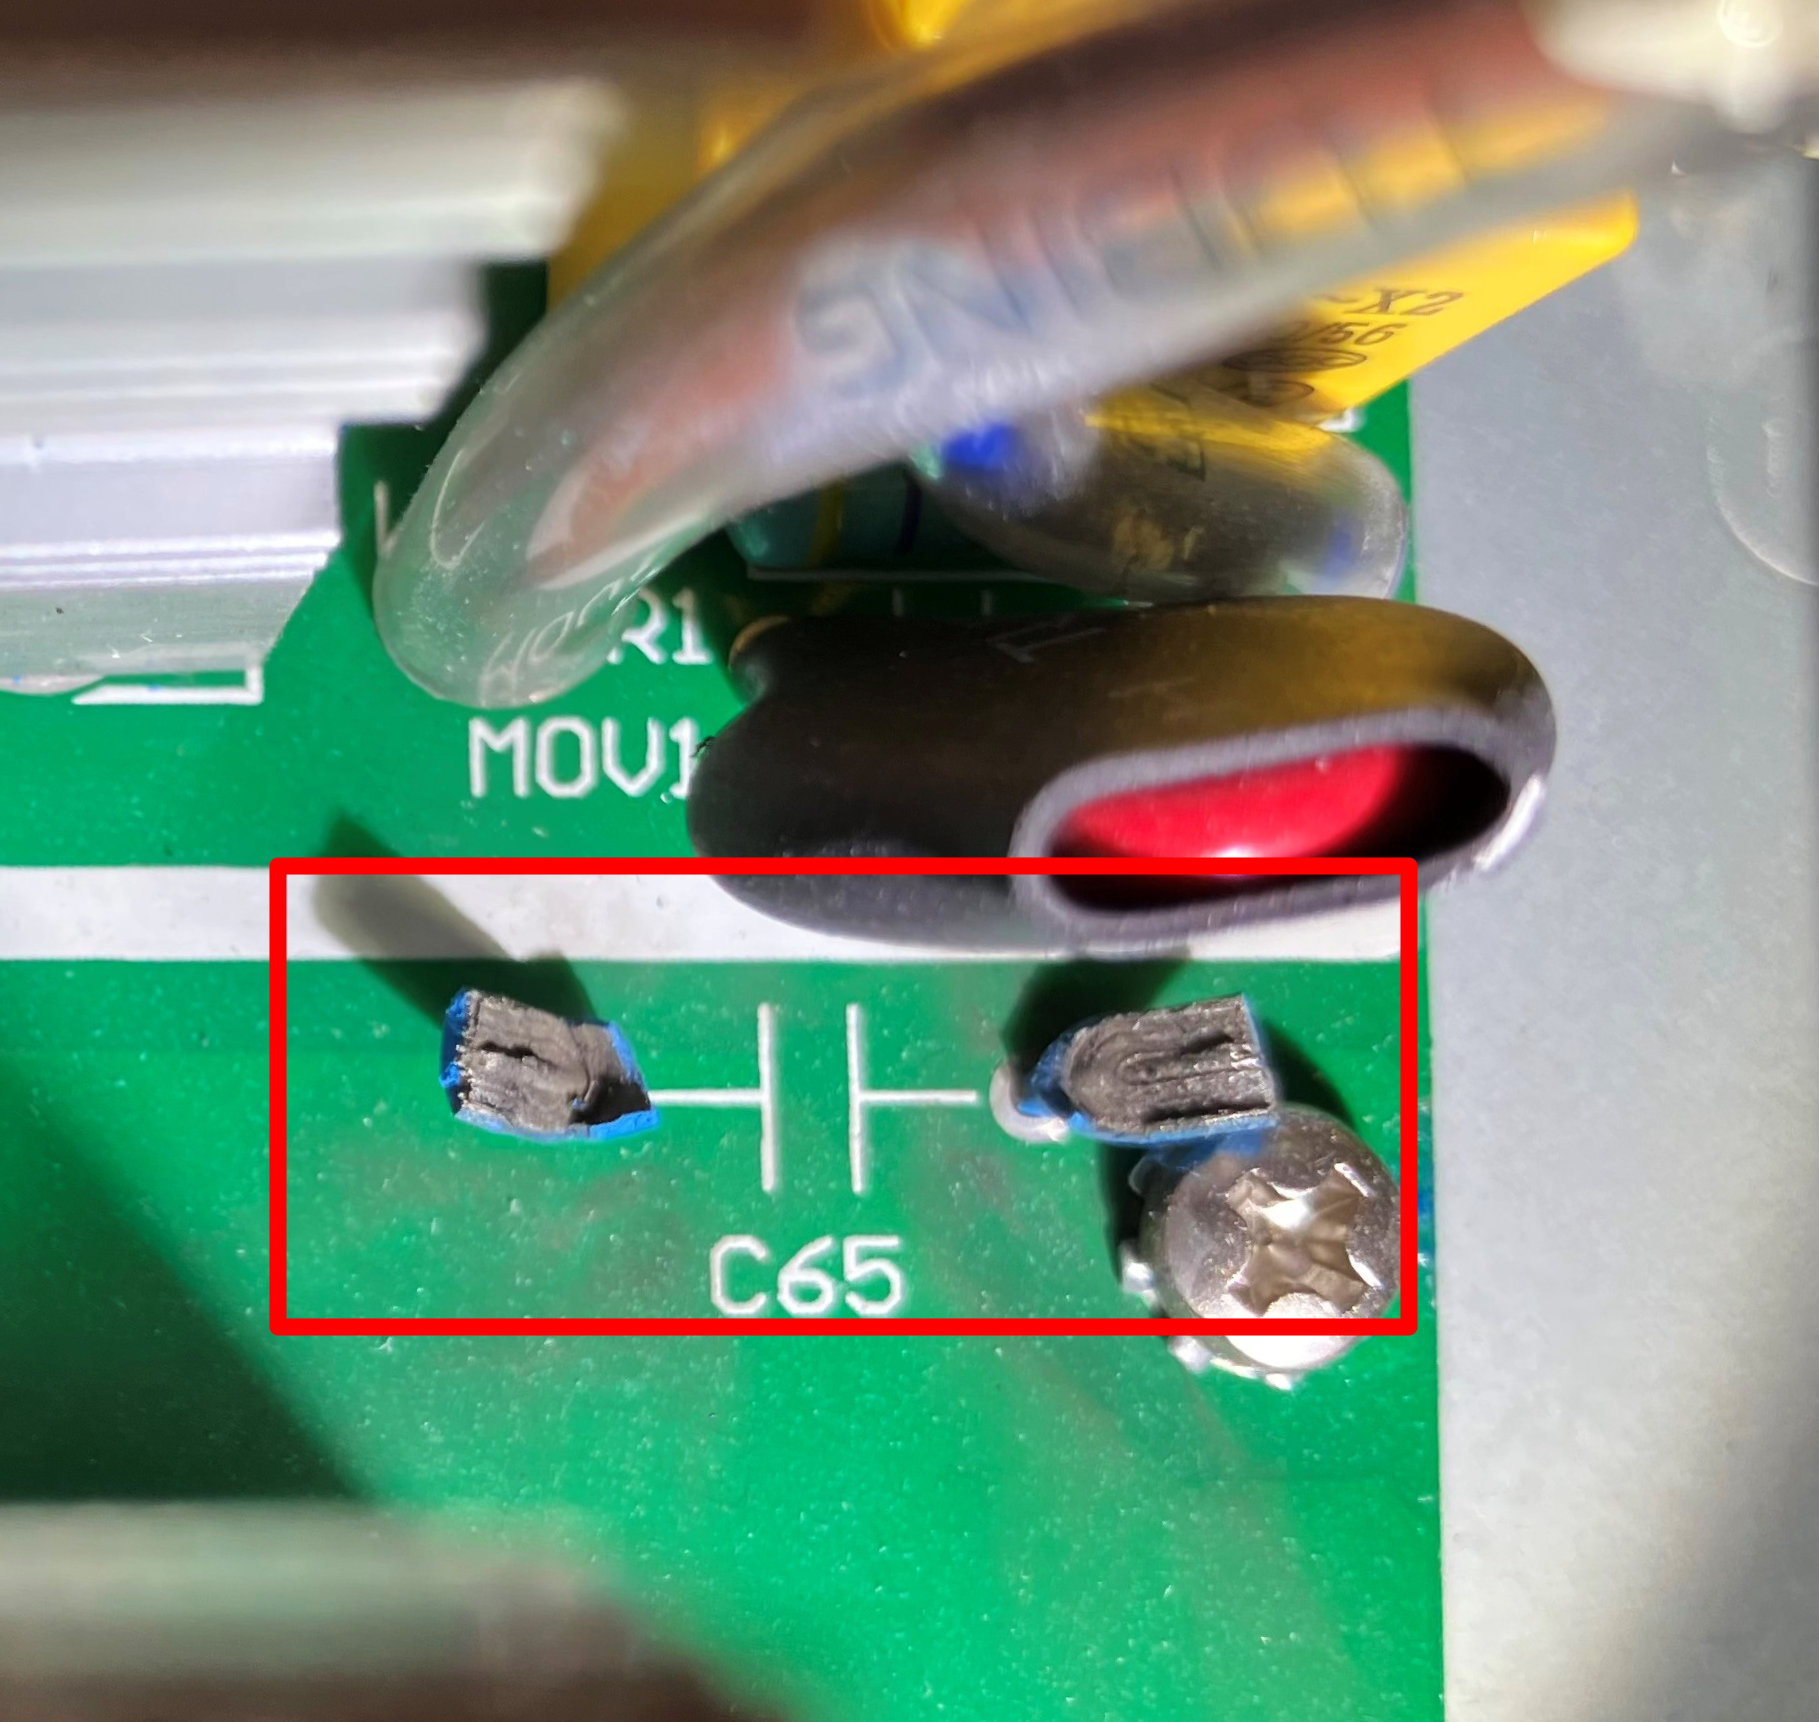
\includegraphics[width=0.85\textwidth]{foto/191}
    \caption{\scriptsize Durch Überspannung völlig zerstörter Kondensator in einem Netzteil. Ursache war ein Blitzeinschlag in der Nähe der Station. Hier kam die Überspannung über das Stromnetz.}
    \label{}
\end{figure}

    \end{column}
   \begin{column}{0.48\textwidth}
       \begin{itemize}
  \item Auch ein Blitz in der Nähe kann durch Überspannung große Schäden anrichten
  \item Ursache ist Induktion in Strom- oder Telefonienetz
  \end{itemize}

   \end{column}
\end{columns}

\end{frame}

\begin{frame}
\frametitle{Blitzschutz}
\begin{columns}
    \begin{column}{0.48\textwidth}
    \begin{itemize}
  \item Blitzschutz-Zwischenstecker für Koaxialkabel mit Gasentladungsröhre
  \item Antennenzuleitung nach dem Funkbetrieb erden, z.B. an Gebäudeerdungsanlage
  \item Dafür ist eine Erdungsleitung notwendig
  \end{itemize}

    \end{column}
   \begin{column}{0.48\textwidth}
       \begin{itemize}
  \item Massiver Draht, keine Litze
  \item Kupfer \qty{16}{\milli\metre}<sup>2</sup>
  \item Aluminium \qty{25}{\milli\metre}<sup>2</sup>
  \item Stahl \qty{50}{\milli\metre}<sup>2</sup>
  \end{itemize}

   \end{column}
\end{columns}

\end{frame}

\begin{frame}
\only<1>{
\begin{QQuestion}{EK209}{Unter welchen Bedingungen darf eine Gebäudeerdungsanlage für die Antennenerdung verwendet werden?}{Jede Gebäudeerdungsanlage kann verwendet werden.}
{Für jede Antenne muss eine separate Erdungsanlage unabhängig von der Gebäudeerdungsanlage aufgebaut werden.}
{Wenn die Gebäudeerdung vom Prüf- und Messdienst der Bundesnetzagentur abgenommen wurde.}
{Die Antennenanlage darf nicht über die von der Gebäudeerdungsanlage eingeschlossenen Fläche hinausragen.}
\end{QQuestion}

}
\only<2>{
\begin{QQuestion}{EK209}{Unter welchen Bedingungen darf eine Gebäudeerdungsanlage für die Antennenerdung verwendet werden?}{\textbf{\textcolor{DARCgreen}{Jede Gebäudeerdungsanlage kann verwendet werden.}}}
{Für jede Antenne muss eine separate Erdungsanlage unabhängig von der Gebäudeerdungsanlage aufgebaut werden.}
{Wenn die Gebäudeerdung vom Prüf- und Messdienst der Bundesnetzagentur abgenommen wurde.}
{Die Antennenanlage darf nicht über die von der Gebäudeerdungsanlage eingeschlossenen Fläche hinausragen.}
\end{QQuestion}

}
\end{frame}

\begin{frame}
\only<1>{
\begin{QQuestion}{EK210}{Welches Material und welcher Mindestquerschnitt kann für eine Erdungsleitung zwischen einem Antennenstandrohr und einer Erdungsanlage nach VDE~0855-300 beispielsweise verwendet werden?}{Ein- oder mehrdrähtiger - aber nicht feindrähtiger - Leiter aus Kupfer~(\qty{10}{\mm\squared}) oder Aluminium~(\qty{16}{\mm\squared}).}
{Einzelmassivdraht aus Kupfer~(\qty{16}{\mm\squared}), Aluminium~(\qty{25}{\mm\squared}) oder Stahl~(\qty{25}{\mm\squared}).}
{Einzelmassivdraht aus Kupfer~(\qty{16}{\mm\squared}), Aluminium~(\qty{25}{\mm\squared}) oder Stahl~(\qty{50}{\mm\squared}).}
{Ein- oder mehrdrähtiger - aber nicht feindrähtiger - Leiter aus Kupfer~(\qty{4}{\mm\squared}) oder Aluminium~(\qty{10}{\mm\squared}).}
\end{QQuestion}

}
\only<2>{
\begin{QQuestion}{EK210}{Welches Material und welcher Mindestquerschnitt kann für eine Erdungsleitung zwischen einem Antennenstandrohr und einer Erdungsanlage nach VDE~0855-300 beispielsweise verwendet werden?}{Ein- oder mehrdrähtiger - aber nicht feindrähtiger - Leiter aus Kupfer~(\qty{10}{\mm\squared}) oder Aluminium~(\qty{16}{\mm\squared}).}
{Einzelmassivdraht aus Kupfer~(\qty{16}{\mm\squared}), Aluminium~(\qty{25}{\mm\squared}) oder Stahl~(\qty{25}{\mm\squared}).}
{\textbf{\textcolor{DARCgreen}{Einzelmassivdraht aus Kupfer~(\qty{16}{\mm\squared}), Aluminium~(\qty{25}{\mm\squared}) oder Stahl~(\qty{50}{\mm\squared}).}}}
{Ein- oder mehrdrähtiger - aber nicht feindrähtiger - Leiter aus Kupfer~(\qty{4}{\mm\squared}) oder Aluminium~(\qty{10}{\mm\squared}).}
\end{QQuestion}

}
\end{frame}

\begin{frame}
\frametitle{Blitzschutzkonzept}
\begin{itemize}
  \item Bei Änderungen an der Blitzschutzanlage eine Blitzschutz-Fachkraft einbeziehen
  \item Insbesondere beim Anschluss von Antennen-Standrohren an die Blitzschutzanlage
  \item Aufnahme der Veränderungen in das Blitzschutzkonzept des Gebäudes
  \end{itemize}
\end{frame}

\begin{frame}
\only<1>{
\begin{QQuestion}{EK211}{Unter welchen Bedingungen darf das Standrohr einer Amateurfunkantenne auf einem Gebäude mit dem gebäudeeigenen Blitzschutzsystem verbunden werden?}{Wenn eine Blitzschutz-Fachkraft die Verbindung des Standrohres der Amateurfunkantenne mit dem Blitzschutzsystem im Blitzschutzkonzept vorsieht.}
{Nach den geltenden Vorschriften muss das Standrohr der Amateurfunkantenne mit einem Gebäudeblitzschutzsystem verbunden werden.}
{Nach den geltenden Vorschriften muss immer ein getrenntes Blitzschutzsystem für die Amateurfunkantenne aufgebaut werden.}
{Wenn für die Verbindungsleitung ein Kupferleiter mit ausreichend großem Querschnitt verwendet wird.}
\end{QQuestion}

}
\only<2>{
\begin{QQuestion}{EK211}{Unter welchen Bedingungen darf das Standrohr einer Amateurfunkantenne auf einem Gebäude mit dem gebäudeeigenen Blitzschutzsystem verbunden werden?}{\textbf{\textcolor{DARCgreen}{Wenn eine Blitzschutz-Fachkraft die Verbindung des Standrohres der Amateurfunkantenne mit dem Blitzschutzsystem im Blitzschutzkonzept vorsieht.}}}
{Nach den geltenden Vorschriften muss das Standrohr der Amateurfunkantenne mit einem Gebäudeblitzschutzsystem verbunden werden.}
{Nach den geltenden Vorschriften muss immer ein getrenntes Blitzschutzsystem für die Amateurfunkantenne aufgebaut werden.}
{Wenn für die Verbindungsleitung ein Kupferleiter mit ausreichend großem Querschnitt verwendet wird.}
\end{QQuestion}

}
\end{frame}%ENDCONTENT


\section{Schutzerdung und Potentialausgleich I}
\label{section:schutzerdung_1}
\begin{frame}%STARTCONTENT

\begin{columns}
    \begin{column}{0.48\textwidth}
    Problem:

\begin{itemize}
  \item Leitfähige Gegenstände können unerwünschte Potentiale (Spannungen) aufweisen
  \item Z.B. elektrische Aufladung, Blitz oder Fehler im Gerät
  \end{itemize}

    \end{column}
   \begin{column}{0.48\textwidth}
       Maßnahmen:

\begin{itemize}
  \item Elektrisch leitende Teile miteinander verbinden
  \item Bei Koaxialkabeln die Schirme miteinander verbinden und an der Haupterdungsschiene anschließen
  \end{itemize}

   \end{column}
\end{columns}

\end{frame}

\begin{frame}
\only<1>{
\begin{QQuestion}{EK208}{Welche Maßnahmen müssen zum Personenschutz bei Koaxialkabeln zur Verhinderung von Spannungsunterschieden ergriffen werden?}{Die Schirme aller Koaxialkabel von Antennen müssen miteinander und mit der Haupterdungsschiene verbunden werden.}
{Für alle Koaxialkabel von Antennen sind Überspannungsableiter vorzusehen.}
{Neben der Erdung des Antennenmastes sind keine weiteren Maßnahmen erforderlich.}
{Die Koaxialkabel müssen ein Schirmungsmaß von mindestens 40 dB aufweisen.}
\end{QQuestion}

}
\only<2>{
\begin{QQuestion}{EK208}{Welche Maßnahmen müssen zum Personenschutz bei Koaxialkabeln zur Verhinderung von Spannungsunterschieden ergriffen werden?}{\textbf{\textcolor{DARCgreen}{Die Schirme aller Koaxialkabel von Antennen müssen miteinander und mit der Haupterdungsschiene verbunden werden.}}}
{Für alle Koaxialkabel von Antennen sind Überspannungsableiter vorzusehen.}
{Neben der Erdung des Antennenmastes sind keine weiteren Maßnahmen erforderlich.}
{Die Koaxialkabel müssen ein Schirmungsmaß von mindestens 40 dB aufweisen.}
\end{QQuestion}

}
\end{frame}%ENDCONTENT


\section{Statische Aufladung von Antennen}
\label{section:statische_aufladung}
\begin{frame}%STARTCONTENT

\begin{columns}
    \begin{column}{0.48\textwidth}
    \begin{itemize}
  \item Unerwünschte Spannungen an Antennen durch statische Aufladungen
  \item Bei ungeerdeten Drahtantennen
  \item Z.B. durch Regen und Hagel
  \item Führt zu Prasselstörungen beim Empfang
  \end{itemize}

    \end{column}
   \begin{column}{0.48\textwidth}
       \begin{itemize}
  \item Abhilfe: Einbringen von Ableitwiderständen zwischen Leitern der Antennenzuführund und der Erdung der Amateurfunkstation
  \item Hochohmig, z.B. 100 kΩ
  \item Dadurch wird die Funktion der Funkanlage nicht beeinträchtigt
  \end{itemize}

   \end{column}
\end{columns}

\end{frame}

\begin{frame}
\only<1>{
\begin{QQuestion}{EK206}{Auf welchen besonderen Sicherheitsaspekt ist speziell bei ungeerdeten Drahtantennen zu achten?}{Durch die fehlende Erdung und den Strombauch im Speisepunkt kann der Mittenisolator zu stark erhitzt werden und durchschmelzen.}
{Durch die Sendeleistung entstehen hohe Spannungen gegen Erde, die eine dickere Isolierung des Antennendrahtes erfordern.}
{Bei Sonnenstürmen entstehen elektrische Aufladungen, die hohe Spannungen erzeugen können.}
{Bereits durch Regen oder Hagel kann es zu elektrischen Aufladungen der Antenne kommen.}
\end{QQuestion}

}
\only<2>{
\begin{QQuestion}{EK206}{Auf welchen besonderen Sicherheitsaspekt ist speziell bei ungeerdeten Drahtantennen zu achten?}{Durch die fehlende Erdung und den Strombauch im Speisepunkt kann der Mittenisolator zu stark erhitzt werden und durchschmelzen.}
{Durch die Sendeleistung entstehen hohe Spannungen gegen Erde, die eine dickere Isolierung des Antennendrahtes erfordern.}
{Bei Sonnenstürmen entstehen elektrische Aufladungen, die hohe Spannungen erzeugen können.}
{\textbf{\textcolor{DARCgreen}{Bereits durch Regen oder Hagel kann es zu elektrischen Aufladungen der Antenne kommen.}}}
\end{QQuestion}

}
\end{frame}

\begin{frame}
\only<1>{
\begin{QQuestion}{EK207}{Wie lassen sich elektrostatische Aufladungen, die insbesondere bei ungeerdeten Drahtantennen auftreten können, wirkungsvoll vermeiden, ohne die Funktion der Funkanlage zu beeinträchtigen?}{Das Einschleifen eines Anpassgerätes zwischen Transceiver und Antenne neutralisiert die Aufladungen.}
{Durch niederohmige Ableitwiderstände zwischen den Anschlüssen an der Antenne und dem Erdanschluss der Amateurfunkstelle.}
{Durch hochohmige Ableitwiderstände zwischen den Anschlüssen an der Antenne und dem Erdanschluss der Amateurfunkstelle.}
{Mit Hilfe der Abblockkondensatoren in einem zwischengeschalteten Stehwellenmessgerät.}
\end{QQuestion}

}
\only<2>{
\begin{QQuestion}{EK207}{Wie lassen sich elektrostatische Aufladungen, die insbesondere bei ungeerdeten Drahtantennen auftreten können, wirkungsvoll vermeiden, ohne die Funktion der Funkanlage zu beeinträchtigen?}{Das Einschleifen eines Anpassgerätes zwischen Transceiver und Antenne neutralisiert die Aufladungen.}
{Durch niederohmige Ableitwiderstände zwischen den Anschlüssen an der Antenne und dem Erdanschluss der Amateurfunkstelle.}
{\textbf{\textcolor{DARCgreen}{Durch hochohmige Ableitwiderstände zwischen den Anschlüssen an der Antenne und dem Erdanschluss der Amateurfunkstelle.}}}
{Mit Hilfe der Abblockkondensatoren in einem zwischengeschalteten Stehwellenmessgerät.}
\end{QQuestion}

}
\end{frame}%ENDCONTENT


\section{Berühren von Antennen I}
\label{section:antennen_beruehrung_1}
\begin{frame}%STARTCONTENT
\emph{Eine Sendeantenne in Betrieb berührt man nicht!}

\begin{itemize}
  \item Hohe Wechselspannungen
  \item Verursachen Herzrhythmusstörungen, Verbrennungen und andere Verletzungen
  \item Kann zum Tod führen
  \item Auch zu Sekundärunfall wie Sturz von der Leiter durch Erschrecken und Verkrampfen
  \end{itemize}
\end{frame}

\begin{frame}
\only<1>{
\begin{QQuestion}{EK202}{Welche möglichen Gefahren bestehen beim Berühren von im Sendebetrieb befindlichen Antennen?}{Keine, da durch den \glqq Skin-Effekt\grqq{} ein Stromfluss durch den menschlichen Körper verhindert wird.}
{Verletzungen und Verbrennungen durch hochfrequente Spannungen.}
{Keine, sofern die Antenne ordnungsgemäß über ein Blitzschutzsystem mit Erde verbunden ist.}
{Stromschlag durch die Gleichspannungsversorgung der Sender-Endstufe, die direkt am Antennenausgang anliegt.}
\end{QQuestion}

}
\only<2>{
\begin{QQuestion}{EK202}{Welche möglichen Gefahren bestehen beim Berühren von im Sendebetrieb befindlichen Antennen?}{Keine, da durch den \glqq Skin-Effekt\grqq{} ein Stromfluss durch den menschlichen Körper verhindert wird.}
{\textbf{\textcolor{DARCgreen}{Verletzungen und Verbrennungen durch hochfrequente Spannungen.}}}
{Keine, sofern die Antenne ordnungsgemäß über ein Blitzschutzsystem mit Erde verbunden ist.}
{Stromschlag durch die Gleichspannungsversorgung der Sender-Endstufe, die direkt am Antennenausgang anliegt.}
\end{QQuestion}

}
\end{frame}%ENDCONTENT


\section{Aufenthalt im Strahlengang}
\label{section:strahlengang_aufenthalt}
\begin{frame}%STARTCONTENT
\begin{itemize}
  \item Insbesondere im Mikrowellenbereich werden Parabol- oder Helixantenen verwendet
  \item Hoher Antennengewinn
  \item Aus wenig Eingangsleistung wird eine hohe Strahlungsleistung
  \item \qty{20}{\dB} sind üblich $\rightarrow$ \qty{1}{\watt} Sendeleistung werden \qty{100}{\watt} Strahlungsleistung
  \end{itemize}

\end{frame}

\begin{frame}\begin{itemize}
  \item Hohe elektromagnetische Felder in der Strahlungskeule
  \item Gefahr für Körper, insbesondere Augen, Gehirn und Hoden
  \item Kann zu Erkrankungen dieser Organe führen
  \item Die Strahlung ist nicht direkt zu spüren
  \item \emph{Der Aufenthalt im direkten Strahlengang von Sendeantennen ist zu vermeiden!}
  \end{itemize}
\end{frame}

\begin{frame}
\only<1>{
\begin{QQuestion}{EK201}{Was ist aus Sicherheitsgründen besonders beim Umgang mit Mikrowellen zu beachten?}{Es ist eine Kopfbedeckung aus Abschirmfolie (z. B. aus Aluminium) zu tragen.}
{Der Duty-Cycle des Senders sollte \qty{50}{\percent} nicht überschreiten.}
{Ein Aufenthalt im direkten Strahlengang von Sendeantennen ist zu vermeiden.}
{Zur Einhaltung des Personenschutzes muss EMV-Schutzkleidung getragen werden.}
\end{QQuestion}

}
\only<2>{
\begin{QQuestion}{EK201}{Was ist aus Sicherheitsgründen besonders beim Umgang mit Mikrowellen zu beachten?}{Es ist eine Kopfbedeckung aus Abschirmfolie (z. B. aus Aluminium) zu tragen.}
{Der Duty-Cycle des Senders sollte \qty{50}{\percent} nicht überschreiten.}
{\textbf{\textcolor{DARCgreen}{Ein Aufenthalt im direkten Strahlengang von Sendeantennen ist zu vermeiden.}}}
{Zur Einhaltung des Personenschutzes muss EMV-Schutzkleidung getragen werden.}
\end{QQuestion}

}

\end{frame}%ENDCONTENT

\end{document}